\documentclass[12pt,a4paper]{book}
\raggedbottom

\usepackage{ugmath_notas}
\usepackage{float}
\usepackage{placeins}
\usepackage[labelfont=bf,labelsep=space]{caption}
\usepackage{pdfpages}
\usepackage{tikz-cd}
\usepackage{amsthm}
\renewcommand{\Tr}{\operatorname{Tr}}
\newcommand{\llaves}[1]{\{#1\}}
\newcommand{\parentesis}[1]{\left(#1\right)}
\newcommand{\corchetes}[1]{\left[#1\right]}
\newcommand{\llavesgrande}[1]{\big\{#1\big\}}
\newcommand{\llavesgrandes}[1]{\left\{#1\right\}}


\begin{document}
        
    
    \thispagestyle{empty}
    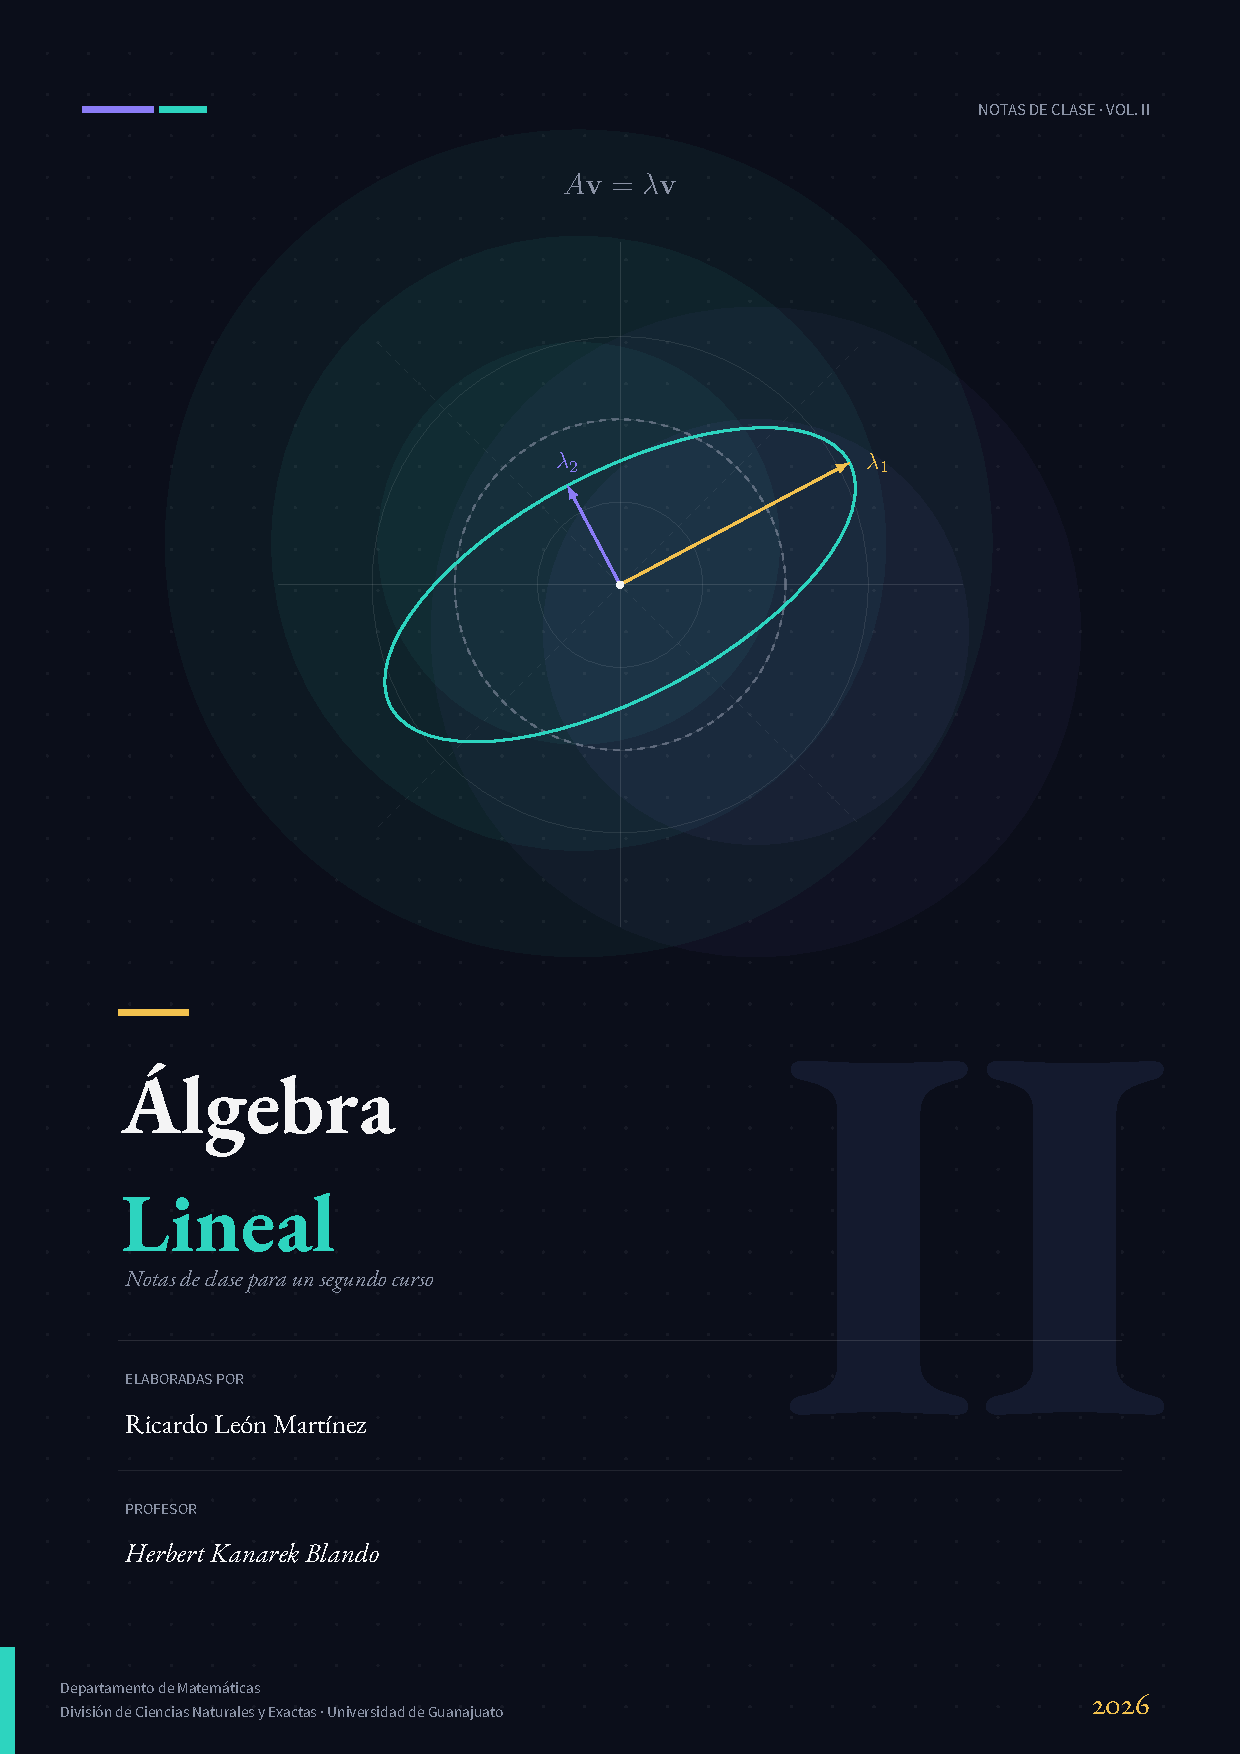
\includepdf[pages=1]{Portada/portada-algebra-lineal-ii.pdf}

    \begin{flushright}
      \thispagestyle{empty}

        \textbf{Ricardo}\\[0.3cm]
        \textit{A los tacos el paisa 2\\
        porque son unos rifados.\\
        A Román porque sufrió redactando\\
        estas notas.\\
        A Uicab por su libreta\\
        de lineal.\\
        Al grupo de todos ínfimos porque\\
        hacen más llevadera la universidad.\\
        Y a Sam, porque aunque no entienda\\
        del todo estas notas,\\
        siempre estuvo ahí.\\
        Y a Kaori, porque entre tareas, estrés\\
        y examenes, también estuvo ahí.}\\[1.2cm]
    \end{flushright}

    % ---------------- NOTA DE ERRORES ----------------

    \cleardoublepage
    \thispagestyle{empty}

    \begin{mdframed}[style=mdgreenbox]
        \begin{center}
        \small
        Estas notas fueron elaboradas con fines académicos.\\
        A pesar del cuidado puesto en su redacción,\\
        es posible que existan errores u omisiones.\\[0.3cm]

        Cualquier corrección, sugerencia o comentario será bienvenido
        en el correo: \\[0.3cm]

        ricardo.leon@cimat.mx
        \end{center}
    \end{mdframed}

    % -------------------------------------------------
    
    \setcounter{page}{1}
    \tableofcontents

    \chapter{Espacios vectoriales}

    \section{Introducción}

    Muchas nociones físicas familiares, como las fuerzas, las velocidades\footnote{La palabra \textit{velocidad} se usa aquí en su sentido científico —como una entidad que tiene tanto magnitud como dirección—. A la magnitud de una velocidad (sin importar la dirección de movimiento) se le llama su \textbf{rapidez}.} y las aceleraciones, involucran tanto una magnitud (la cantidad de fuerza, velocidad o aceleración) como una dirección. Cualquier entidad que involucre magnitud y dirección se llama \textbf{vector}. Un vector se representa mediante una flecha cuya longitud denota la magnitud del vector, y cuya dirección representa la dirección del vector. En la mayoría de las situaciones físicas que involucran vectores, solo son significativas la magnitud y la dirección del vector; en consecuencia, consideramos iguales a los vectores que tienen la misma magnitud y dirección, sin importar sus posiciones. En esta sección se analiza la geometría de los vectores. Esta geometría se deriva de experimentos físicos que examinan la manera en que interactúan dos vectores.

    Situaciones familiares sugieren que, cuando dos cantidades físicas semejantes actúan simultáneamente en un punto, la magnitud de su efecto conjunto no necesariamente es igual a la suma de las magnitudes de las cantidades originales. Por ejemplo, un nadador que nada río arriba a una velocidad de $2$ millas por hora contra una corriente de $1$ milla por hora no avanza a razón de $3$ millas por hora. En este caso, los movimientos del nadador y de la corriente se oponen entre sí, y la rapidez de avance del nadador es de solo $1$ milla por hora río arriba. Si, en cambio, el nadador se mueve río abajo (con la corriente), entonces su rapidez de avance es de $3$ millas por hora río abajo.

    Los experimentos muestran que, si dos cantidades semejantes actúan juntas, su efecto es predecible. En este caso, los vectores que representan estas cantidades pueden combinarse para formar un vector resultante que representa el efecto combinado de las cantidades originales. A este vector resultante se le llama la \textbf{suma} de los vectores originales, y a la regla para su combinación se le llama la \textbf{ley del paralelogramo}.

    \begin{figure}[H]
        \centering
        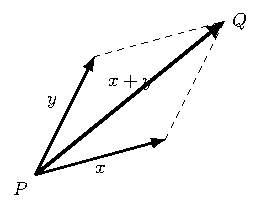
\includegraphics[width=0.4\textwidth]{figuras/ley-paralelogramo.pdf}
        \caption{Ley del paralelogramo para la suma de vectores.}
    \end{figure}

    \begin{definicion}[Ley del paralelogramo para la suma de vectores]
        La \textbf{suma} de dos vectores $x$ y $y$ que actúan en el mismo punto $P$ es el vector que comienza en $P$ y está representado por la diagonal del paralelogramo que tiene a $x$ y a $y$ como lados adyacentes.
    \end{definicion}

    Como los lados opuestos de un paralelogramo son paralelos y de igual longitud, el extremo $Q$ de la flecha que representa a $x+y$ también puede obtenerse dejando actuar a $x$ en $P$ y luego dejando actuar a $y$ en el extremo de $x$. De manera análoga, el extremo del vector $x+y$ puede obtenerse haciendo actuar primero a $y$ en $P$, y luego a $x$ en el extremo de $y$. Así, los dos vectores $x$ y $y$, ambos actuando en el punto $P$, pueden sumarse \textquotedblleft de cola a punta\textquotedblright; es decir, cualquiera de los dos, $x$ o $y$, puede aplicarse en $P$, y un vector con la misma magnitud y dirección que el otro puede aplicarse en el extremo del primero. Si esto se hace, el extremo del segundo vector es el extremo de $x+y$.

    La suma de vectores puede describirse algebraicamente con ayuda de la geometría analítica. En el plano que contiene a $x$ y a $y$, introduzcamos un sistema de coordenadas con $P$ en el origen. Sean $(a_1,a_2)$ el extremo de $x$ y $(b_1,b_2)$ el extremo de $y$. Entonces, como muestra la Figura 1.2(a), el extremo $Q$ de $x+y$ es $(a_1+b_1,a_2+b_2)$. En adelante, cuando se haga referencia a las coordenadas del extremo de un vector, se supondrá que el vector emana del origen. Más aún, como un vector que comienza en el origen queda completamente determinado por su extremo, a veces nos referiremos \textit{al punto $x$} en lugar de \textit{al extremo del vector $x$}, si $x$ es un vector que emana del origen.

    Además de la operación de suma de vectores, existe otra operación natural que puede realizarse sobre vectores: la longitud de un vector puede magnificarse o contraerse. Esta operación, llamada \textbf{multiplicación por escalar}, consiste en multiplicar el vector por un número real. Si el vector $x$ está representado por una flecha, entonces, para cualquier número real $t$, el vector $tx$ está representado por una flecha en la misma dirección si $t\geq 0$ y en la dirección opuesta si $t<0$. La longitud de la flecha $tx$ es $|t|$ veces la longitud de la flecha $x$. Dos vectores no nulos $x$ y $y$ se llaman \textbf{paralelos} si $y=tx$ para algún número real no nulo $t$. (Así, dos vectores no nulos que tienen la misma dirección o direcciones opuestas son paralelos.)

    Para describir algebraicamente la multiplicación por escalar, introduzcamos de nuevo un sistema de coordenadas en un plano que contenga al vector $x$, de modo que $x$ emane del origen. Si el extremo de $x$ tiene coordenadas $(a_1,a_2)$, se ve fácilmente que las coordenadas del extremo de $tx$ son $(ta_1,ta_2)$. (Véase la Figura 1.2(b).)

    \begin{figure}[H]
        \centering
        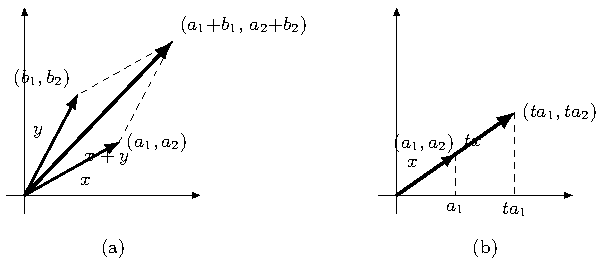
\includegraphics[width=0.85\textwidth]{figuras/suma-y-escalar-coordenadas.pdf}
        \caption{(a) Suma de vectores en coordenadas. (b) Multiplicación por escalar en coordenadas.}
    \end{figure}

    Las descripciones algebraicas de la suma de vectores y la multiplicación por escalar para vectores en un plano producen las siguientes propiedades:
    \begin{enumerate}
        \item Para todos los vectores $x$ y $y$, $x+y=y+x$.
        \item Para todos los vectores $x$, $y$ y $z$, $(x+y)+z=x+(y+z)$.
        \item Existe un vector, denotado $0$, tal que $x+0=x$ para todo vector $x$.
        \item Para todo vector $x$, existe un vector $y$ tal que $x+y=0$.
        \item Para todo vector $x$, $1x=x$.
        \item Para cada par de números reales $a$ y $b$, y para todo vector $x$, $(ab)x=a(bx)$.
        \item Para cada número real $a$ y cada par de vectores $x$ y $y$, $a(x+y)=ax+ay$.
        \item Para cada par de números reales $a$ y $b$, y para todo vector $x$, $(a+b)x=ax+bx$.
    \end{enumerate}

    Argumentos similares a los anteriores muestran que estas ocho propiedades, así como las interpretaciones geométricas de la suma de vectores y la multiplicación por escalar, también son válidas para vectores que actúan en el espacio en vez de en un plano. Estos resultados pueden usarse para escribir ecuaciones de rectas y planos en el espacio.

    Consideremos primero la ecuación de una recta en el espacio que pasa por dos puntos distintos $A$ y $B$. Sea $O$ el origen de un sistema de coordenadas en el espacio, y sean $u$ y $v$ los vectores que comienzan en $O$ y terminan en $A$ y en $B$, respectivamente. Si $w$ denota el vector que comienza en $A$ y termina en $B$, entonces la suma \textquotedblleft de cola a punta\textquotedblright\ muestra que $u+w=v$, y por tanto $w=v-u$, donde $-u$ denota el vector $(-1)u$. (Véase la Figura 1.3, en la cual el cuadrilátero $OABC$ es un paralelogramo, siendo $C$ el punto tal que el vector que emana de $O$ y termina en $C$ es $v-u$.) Como un múltiplo escalar de $w$ es paralelo a $w$, pero posiblemente de longitud distinta, cualquier punto de la recta que une a $A$ con $B$ puede obtenerse como el extremo de un vector que comienza en $A$ y tiene la forma $tw$, para algún número real $t$. Recíprocamente, el extremo de todo vector de la forma $tw$ que comienza en $A$ está sobre la recta que une a $A$ con $B$. Así, una ecuación de la recta que pasa por $A$ y $B$ es
    \begin{equation*}
        x=u+tw=u+t(v-u),
    \end{equation*}
    donde $t$ es un número real y $x$ denota un punto arbitrario de la recta. Notemos también que el extremo $C$ del vector $v-u$ en la Figura 1.3 tiene coordenadas iguales a la diferencia de las coordenadas de $B$ y de $A$.

    \begin{figure}[H]
        \centering
        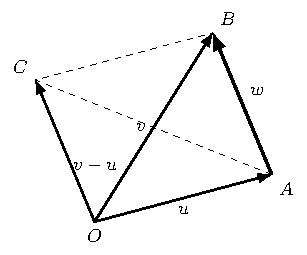
\includegraphics[width=0.5\textwidth]{figuras/recta-por-dos-puntos.pdf}
        \caption{La recta por $A$ y $B$, y el paralelogramo $OABC$.}
    \end{figure}

    \begin{ejemplo}
        Sean $A$ y $B$ los puntos con coordenadas $(-2,0,1)$ y $(4,5,3)$, respectivamente. El extremo $C$ del vector que emana del origen y tiene la misma dirección que el vector que comienza en $A$ y termina en $B$ tiene coordenadas $(4,5,3)-(-2,0,1)=(6,5,2)$. Por tanto la ecuación de la recta por $A$ y $B$ es
        \begin{equation*}
            x=(-2,0,1)+t(6,5,2).
        \end{equation*}
    \end{ejemplo}

    Sean ahora $A$, $B$ y $C$ tres puntos cualesquiera, no colineales, en el espacio. Estos puntos determinan un único plano, y su ecuación puede encontrarse usando nuestras observaciones previas sobre vectores. Sean $u$ y $v$ vectores que comienzan en $A$ y terminan en $B$ y en $C$, respectivamente. Observemos que cualquier punto del plano que contiene a $A$, $B$ y $C$ es el extremo $S$ de un vector $x$ que comienza en $A$ y tiene la forma $su+tv$, para algunos números reales $s$ y $t$. El extremo de $su$ es el punto de intersección de la recta por $A$ y $B$ con la recta por $S$ paralela a la recta por $A$ y $C$. Un procedimiento similar ubica el extremo de $tv$. Más aún, para cualesquiera números reales $s$ y $t$, el vector $su+tv$ está contenido en el plano que contiene a $A$, $B$ y $C$. Se sigue que una ecuación del plano que contiene a $A$, $B$ y $C$ es
    \begin{equation*}
        x=A+su+tv,
    \end{equation*}
    donde $s$ y $t$ son números reales arbitrarios y $x$ denota un punto arbitrario del plano.

    \begin{figure}[H]
        \centering
        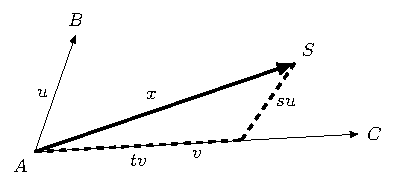
\includegraphics[width=0.6\textwidth]{figuras/plano-por-tres-puntos.pdf}
        \caption{El plano que contiene a $A$, $B$ y $C$.}
    \end{figure}

    \begin{ejemplo}
        Sean $A$, $B$ y $C$ los puntos con coordenadas $(1,0,2)$, $(-3,-2,4)$ y $(1,8,-5)$, respectivamente. El extremo del vector que emana del origen y tiene la misma longitud y dirección que el vector que comienza en $A$ y termina en $B$ es
        \begin{equation*}
            (-3,-2,4)-(1,0,2)=(-4,-2,2).
        \end{equation*}
        De manera análoga, el extremo del vector que emana del origen y tiene la misma longitud y dirección que el vector que comienza en $A$ y termina en $C$ es $(1,8,-5)-(1,0,2)=(0,8,-7)$. Por tanto la ecuación del plano que contiene a los tres puntos dados es
        \begin{equation*}
            x=(1,0,2)+s(-4,-2,2)+t(0,8,-7).
        \end{equation*}
    \end{ejemplo}

    A cualquier estructura matemática que posea las ocho propiedades enunciadas en esta sección se le llama \textit{espacio vectorial}. En la siguiente sección definimos formalmente un espacio vectorial y consideramos muchos ejemplos de espacios vectoriales distintos de los mencionados anteriormente.

    \begin{ejercicio}
        Determine si los vectores que emanan del origen y terminan en los siguientes pares de puntos son paralelos.
        \begin{enumerate}[label=(\alph*)]
            \item $(3,1,2)$ y $(6,4,2)$
            \item $(-3,1,7)$ y $(9,-3,-21)$
            \item $(5,-6,7)$ y $(-5,6,-7)$
            \item $(2,0,-5)$ y $(5,0,-2)$
        \end{enumerate}
    \end{ejercicio}

    \begin{ejercicio}
        Encuentre las ecuaciones de las rectas que pasan por los siguientes pares de puntos en el espacio.
        \begin{enumerate}[label=(\alph*)]
            \item $(3,-2,4)$ y $(-5,7,1)$
            \item $(2,4,0)$ y $(-3,-6,0)$
            \item $(3,7,2)$ y $(3,7,-8)$
            \item $(-2,-1,5)$ y $(3,9,7)$
        \end{enumerate}
    \end{ejercicio}

    \begin{ejercicio}
        Encuentre las ecuaciones de los planos que contienen a los siguientes puntos.
        \begin{enumerate}[label=(\alph*)]
            \item $(2,-5,-1)$, $(0,4,6)$ y $(-3,7,1)$
            \item $(3,-6,7)$, $(-2,0,-4)$ y $(5,-9,-2)$
            \item $(-8,2,0)$, $(1,3,0)$ y $(6,-5,0)$
            \item $(1,1,1)$, $(5,5,5)$ y $(-6,4,2)$
        \end{enumerate}
    \end{ejercicio}

    \begin{ejercicio}
        ¿Cuáles son las coordenadas del vector $0$ en el plano euclidiano que satisface la propiedad 3 de esta sección? Justifique su respuesta.
    \end{ejercicio}

    \begin{ejercicio}
        Pruebe que, si el vector $x$ emana del origen del plano euclidiano y termina en el punto con coordenadas $(a_1,a_2)$, entonces el vector $tx$ que emana del origen termina en el punto con coordenadas $(ta_1,ta_2)$.
    \end{ejercicio}

    \begin{ejercicio}
        Muestre que el punto medio del segmento que une a los puntos $(a,b)$ y $(c,d)$ es $\big((a+c)/2,(b+d)/2\big)$.
    \end{ejercicio}

    \begin{ejercicio}
        Pruebe que las diagonales de un paralelogramo se bisecan entre sí.
    \end{ejercicio}

    \section{Espacios vectoriales}

    En la Sección~1.1 vimos que, con las definiciones naturales de suma de vectores y multiplicación por escalar, los vectores en un plano satisfacen las ocho propiedades enunciadas en la página anterior. Muchos otros sistemas algebraicos familiares también admiten definiciones de suma y multiplicación por escalar que satisfacen las mismas ocho propiedades. En esta sección presentamos algunos de estos sistemas, pero antes definimos formalmente este tipo de estructura algebraica.

    \begin{definicion}[Espacio vectorial]
        Un \textbf{espacio vectorial} (o \textbf{espacio lineal}) $V$ sobre un campo $F$ consiste de un conjunto sobre el cual se definen dos operaciones (llamadas \textbf{suma} y \textbf{multiplicación por escalar}, respectivamente), de modo que para cada par de elementos $x,y$ en $V$ existe un único elemento $x+y$ en $V$, y para cada elemento $a$ en $F$ y cada elemento $x$ en $V$ existe un único elemento $ax$ en $V$, tales que se cumplen las siguientes condiciones:
        \begin{enumerate}
            \item[(EV 1)] Para todos $x,y\in V$, $x+y=y+x$ (conmutatividad de la suma).
            \item[(EV 2)] Para todos $x,y,z\in V$, $(x+y)+z=x+(y+z)$ (asociatividad de la suma).
            \item[(EV 3)] Existe un elemento en $V$, denotado $0$, tal que $x+0=x$ para todo $x\in V$.
            \item[(EV 4)] Para cada elemento $x\in V$, existe un elemento $y\in V$ tal que $x+y=0$.
            \item[(EV 5)] Para cada elemento $x\in V$, $1x=x$.
            \item[(EV 6)] Para cada par de elementos $a,b\in F$ y cada $x\in V$, $(ab)x=a(bx)$.
            \item[(EV 7)] Para cada $a\in F$ y cada par de elementos $x,y\in V$, $a(x+y)=ax+ay$.
            \item[(EV 8)] Para cada par de elementos $a,b\in F$ y cada $x\in V$, $(a+b)x=ax+bx$.
        \end{enumerate}
        A los elementos $x+y$ y $ax$ se les llama, respectivamente, la \textbf{suma} de $x$ y $y$, y el \textbf{producto} de $a$ y $x$.
    \end{definicion}

    A los elementos del campo $F$ se les llama \textbf{escalares}, y a los elementos del espacio vectorial $V$ se les llama \textbf{vectores}. El lector no debe confundir este uso de la palabra \textquotedblleft vector\textquotedblright\ con la entidad física discutida en la Sección~1.1: la palabra \textquotedblleft vector\textquotedblright\ ya no se usa aquí para describir necesariamente una entidad con magnitud y dirección, sino cualquier elemento de un espacio vectorial.

    Un espacio vectorial se discute frecuentemente sin mencionar explícitamente su campo de escalares. El lector debe recordar, sin embargo, que todo espacio vectorial se considera como un espacio vectorial sobre un campo dado, el cual se denota por $F$. En ocasiones restringimos nuestra atención a los campos de los números reales y complejos, denotados $\R$ y $\C$, respectivamente.

    Observemos que (EV 2) nos permite definir sin ambigüedad la suma de cualquier número finito de vectores (sin el uso de paréntesis).

    En el resto de esta sección presentamos varios ejemplos importantes de espacios vectoriales que se estudian a lo largo de estas notas. Observemos que, al describir un espacio vectorial, es necesario especificar no solo los vectores, sino también las operaciones de suma y multiplicación por escalar.

    Un objeto de la forma $(a_1,a_2,\dots,a_n)$, donde las entradas $a_1,a_2,\dots,a_n$ son elementos de un campo $F$, se llama una \textbf{$n$-ada} con entradas en $F$. Las entradas $a_1,a_2,\dots,a_n$ se llaman las \textbf{entradas} o \textbf{componentes} de la $n$-ada. Dos $n$-adas $(a_1,a_2,\dots,a_n)$ y $(b_1,b_2,\dots,b_n)$ con entradas en $F$ se llaman \textbf{iguales} si $a_i=b_i$ para $i=1,2,\dots,n$.

    \begin{ejemplo}
        El conjunto de todas las $n$-adas con entradas en un campo $F$ se denota $F^n$. Este conjunto es un espacio vectorial sobre $F$ con las operaciones de suma y multiplicación por escalar coordenada a coordenada; es decir, si $u=(a_1,a_2,\dots,a_n)\in F^n$, $v=(b_1,b_2,\dots,b_n)\in F^n$, y $c\in F$, entonces
        \begin{equation*}
            u+v=(a_1+b_1,a_2+b_2,\dots,a_n+b_n) \qquad\text{y}\qquad cu=(ca_1,ca_2,\dots,ca_n).
        \end{equation*}
        Así $\R^3$ es un espacio vectorial sobre $\R$. En este espacio vectorial,
        \begin{equation*}
            (3,-2,0)+(-1,1,4)=(2,-1,4) \qquad\text{y}\qquad -5(1,-2,0)=(-5,10,0).
        \end{equation*}
        Análogamente, $\C^2$ es un espacio vectorial sobre $\C$. En este espacio vectorial,
        \begin{equation*}
            (1+i,2)+(2-3i,4i)=(3-2i,2+4i) \qquad\text{y}\qquad i(1+i,2)=(-1+i,2i).
        \end{equation*}
        Los vectores en $F^n$ pueden escribirse como \textbf{vectores columna}
        \begin{equation*}
            \begin{pmatrix}a_1\\a_2\\\vdots\\a_n\end{pmatrix}
        \end{equation*}
        en lugar de \textbf{vectores renglón} $(a_1,a_2,\dots,a_n)$. Como una $1$-ada cuya única entrada está en $F$ puede considerarse como un elemento de $F$, usualmente escribimos $F$ en lugar de $F^1$ para el espacio vectorial de $1$-adas con entrada en $F$.
    \end{ejemplo}

    Una \textbf{matriz} $m\times n$ con entradas en un campo $F$ es un arreglo rectangular de la forma
    \begin{equation*}
        \begin{pmatrix}a_{11}&a_{12}&\cdots&a_{1n}\\a_{21}&a_{22}&\cdots&a_{2n}\\\vdots&\vdots&&\vdots\\a_{m1}&a_{m2}&\cdots&a_{mn}\end{pmatrix},
    \end{equation*}
    donde cada entrada $a_{ij}$ ($1\leq i\leq m$, $1\leq j\leq n$) es un elemento de $F$. A las entradas $a_{ij}$ con $i=j$ se les llama las \textbf{entradas diagonales} de la matriz. Las entradas $a_{i1},a_{i2},\dots,a_{in}$ forman el \textbf{$i$-ésimo renglón} de la matriz, y las entradas $a_{1j},a_{2j},\dots,a_{mj}$ forman la \textbf{$j$-ésima columna} de la matriz. Los renglones de la matriz anterior se consideran como vectores en $F^n$, y las columnas se consideran como vectores en $F^m$. A la matriz $m\times n$ en la que cada entrada es igual a cero se le llama \textbf{matriz cero} y se denota $O$.

    En estas notas, denotamos las matrices con letras mayúsculas cursivas (por ejemplo, $A$, $B$ y $C$), y denotamos la entrada de una matriz $A$ que está en el renglón $i$ y la columna $j$ por $A_{ij}$. Además, si el número de renglones y de columnas de una matriz es el mismo, la matriz se llama \textbf{cuadrada}. Dos matrices $A$ y $B$, ambas de tamaño $m\times n$, se llaman \textbf{iguales} si todas sus entradas correspondientes son iguales, es decir, si $A_{ij}=B_{ij}$ para $1\leq i\leq m$ y $1\leq j\leq n$.

    \begin{ejemplo}
        El conjunto de todas las matrices $m\times n$ con entradas en un campo $F$ es un espacio vectorial, que denotamos $M_{m\times n}(F)$, con las siguientes operaciones de \textbf{suma de matrices} y \textbf{multiplicación por escalar}: para $A,B\in M_{m\times n}(F)$ y $c\in F$,
        \begin{equation*}
            (A+B)_{ij}=A_{ij}+B_{ij} \qquad\text{y}\qquad (cA)_{ij}=cA_{ij}
        \end{equation*}
        para $1\leq i\leq m$ y $1\leq j\leq n$. Por ejemplo,
        \begin{equation*}
            \begin{pmatrix}2&0&-1\\1&-3&4\end{pmatrix}+\begin{pmatrix}-5&-2&6\\3&4&-1\end{pmatrix}=\begin{pmatrix}-3&-2&5\\4&1&3\end{pmatrix}
        \end{equation*}
        y
        \begin{equation*}
            -3\begin{pmatrix}1&0&-2\\-3&2&3\end{pmatrix}=\begin{pmatrix}-3&0&6\\9&-6&-9\end{pmatrix}
        \end{equation*}
        en $M_{2\times 3}(\R)$.
    \end{ejemplo}

    \begin{ejemplo}
        Sea $S$ cualquier conjunto no vacío y $F$ cualquier campo, y sea $\mathcal{F}(S,F)$ el conjunto de todas las funciones de $S$ en $F$. Dos funciones $f$ y $g$ en $\mathcal{F}(S,F)$ se llaman \textbf{iguales} si $f(s)=g(s)$ para todo $s\in S$. El conjunto $\mathcal{F}(S,F)$ es un espacio vectorial con las operaciones de suma y multiplicación por escalar definidas, para $f,g\in\mathcal{F}(S,F)$ y $c\in F$, por
        \begin{equation*}
            (f+g)(s)=f(s)+g(s) \qquad\text{y}\qquad (cf)(s)=c[f(s)]
        \end{equation*}
        para cada $s\in S$. Notemos que estas son las operaciones familiares de suma y multiplicación por escalar para funciones, usadas en álgebra y en cálculo.
    \end{ejemplo}

    Un \textbf{polinomio} con coeficientes en un campo $F$ es una expresión de la forma
    \begin{equation*}
        f(x)=a_nx^n+a_{n-1}x^{n-1}+\cdots+a_1x+a_0,
    \end{equation*}
    donde $n$ es un entero no negativo y cada $a_k$, llamado el \textbf{coeficiente} de $x^k$, está en $F$. Si $f(x)=0$, es decir, si $a_n=a_{n-1}=\cdots=a_0=0$, entonces $f(x)$ se llama el \textbf{polinomio cero} y, por convención, su grado se define como $-1$; en cualquier otro caso, el \textbf{grado} de un polinomio se define como el mayor exponente de $x$ que aparece en la representación
    \begin{equation*}
        f(x)=a_nx^n+a_{n-1}x^{n-1}+\cdots+a_1x+a_0
    \end{equation*}
    con coeficiente no nulo. Notemos que los polinomios de grado cero pueden escribirse en la forma $f(x)=c$ para algún escalar no nulo $c$. Dos polinomios,
    \begin{equation*}
        f(x)=a_nx^n+a_{n-1}x^{n-1}+\cdots+a_1x+a_0 \qquad\text{y}\qquad g(x)=b_mx^m+b_{m-1}x^{m-1}+\cdots+b_1x+b_0,
    \end{equation*}
    se llaman \textbf{iguales} si $m=n$ y $a_i=b_i$ para $i=0,1,\dots,n$.

    Cuando $F$ es un campo con una infinidad de escalares, usualmente consideramos un polinomio con coeficientes en $F$ como una función de $F$ en $F$. En este caso, el valor de la función
    \begin{equation*}
        f(x)=a_nx^n+a_{n-1}x^{n-1}+\cdots+a_1x+a_0
    \end{equation*}
    en $c\in F$ es el escalar
    \begin{equation*}
        f(c)=a_nc^n+a_{n-1}c^{n-1}+\cdots+a_1c+a_0.
    \end{equation*}
    Aquí se usa cualquiera de las notaciones $f$ o $f(x)$ para la función polinomial $f(x)=a_nx^n+a_{n-1}x^{n-1}+\cdots+a_1x+a_0$.

    \begin{ejemplo}
        Sean
        \begin{equation*}
            f(x)=a_nx^n+a_{n-1}x^{n-1}+\cdots+a_1x+a_0 \qquad\text{y}\qquad g(x)=b_mx^m+b_{m-1}x^{m-1}+\cdots+b_1x+b_0
        \end{equation*}
        polinomios con coeficientes en un campo $F$. Supongamos que $m\leq n$, y definamos $b_{m+1}=b_{m+2}=\cdots=b_n=0$. Entonces $g(x)$ puede escribirse como
        \begin{equation*}
            g(x)=b_nx^n+b_{n-1}x^{n-1}+\cdots+b_1x+b_0.
        \end{equation*}
        Definamos
        \begin{equation*}
            f(x)+g(x)=(a_n+b_n)x^n+(a_{n-1}+b_{n-1})x^{n-1}+\cdots+(a_1+b_1)x+(a_0+b_0)
        \end{equation*}
        y, para cualquier $c\in F$, definamos
        \begin{equation*}
            cf(x)=ca_nx^n+ca_{n-1}x^{n-1}+\cdots+ca_1x+ca_0.
        \end{equation*}
        Con estas operaciones de suma y multiplicación por escalar, el conjunto de todos los polinomios con coeficientes en $F$ es un espacio vectorial, que denotamos $P(F)$.
    \end{ejemplo}

    Veremos más adelante que el espacio vectorial definido en el siguiente ejemplo es, en esencia, el mismo que $P(F)$.

    \begin{ejemplo}
        Sea $F$ cualquier campo. Una \textbf{sucesión} en $F$ es una función $\sigma$ de los enteros positivos en $F$. En estas notas, la sucesión $\sigma$ tal que $\sigma(n)=a_n$ para $n=1,2,\dots$ se denota $\{a_n\}$. Sea $V$ el conjunto de todas las sucesiones $\{a_n\}$ en $F$ que tienen solo un número finito de términos $a_n$ no nulos. Si $\{a_n\}$ y $\{b_n\}$ están en $V$ y $t\in F$, definamos
        \begin{equation*}
            \{a_n\}+\{b_n\}=\{a_n+b_n\} \qquad\text{y}\qquad t\{a_n\}=\{ta_n\}.
        \end{equation*}
        Con estas operaciones, $V$ es un espacio vectorial.
    \end{ejemplo}

    Nuestros siguientes dos ejemplos contienen conjuntos en los que se definen operaciones de suma y multiplicación por escalar, pero que \textit{no} son espacios vectoriales.

    \begin{ejemplo}
        Sea $S=\{(a_1,a_2):a_1,a_2\in\R\}$. Para $(a_1,a_2),(b_1,b_2)\in S$ y $c\in\R$, definamos
        \begin{equation*}
            (a_1,a_2)+(b_1,b_2)=(a_1+b_1,\,a_2-b_2) \qquad\text{y}\qquad c(a_1,a_2)=(ca_1,ca_2).
        \end{equation*}
        Como (EV 1), (EV 2) y (EV 8) fallan, $S$ no es un espacio vectorial con estas operaciones.
    \end{ejemplo}

    \begin{ejemplo}
        Sea $S$ como en el ejemplo anterior. Para $(a_1,a_2),(b_1,b_2)\in S$ y $c\in\R$, definamos
        \begin{equation*}
            (a_1,a_2)+(b_1,b_2)=(a_1+b_1,0) \qquad\text{y}\qquad c(a_1,a_2)=(ca_1,0).
        \end{equation*}
        Entonces $S$ no es un espacio vectorial con estas operaciones porque (EV 3) (y en consecuencia (EV 4)) y (EV 5) fallan.
    \end{ejemplo}

    Concluimos esta sección con algunas consecuencias elementales de la definición de espacio vectorial.

    \begin{teorema}[Ley de cancelación para la suma de vectores]
        Si $x$, $y$ y $z$ son vectores de un espacio vectorial $V$ tales que $x+z=y+z$, entonces $x=y$.
    \end{teorema}

    \begin{proof}
        Existe un vector $v\in V$ tal que $z+v=0$ (EV 4). Así,
        \begin{align*}
            x&=x+0=x+(z+v)=(x+z)+v\\
            &=(y+z)+v=y+(z+v)=y+0=y
        \end{align*}
        por (EV 2) y (EV 3).
    \end{proof}

    \begin{corolario}
        El vector $0$ descrito en (EV 3) es único.
    \end{corolario}

    \begin{proof}
        Supongamos que $0$ y $0'$ satisfacen ambos (EV 3); es decir, $x+0=x$ y $x+0'=x$ para todo $x\in V$. En particular, tomando $x=0'$ en la primera igualdad y $x=0$ en la segunda,
        \begin{equation*}
            0'+0=0' \qquad\text{y}\qquad 0+0'=0.
        \end{equation*}
        Por (EV 1), $0'+0=0+0'$; por tanto $0'=0$.
    \end{proof}

    \begin{corolario}
        El vector $y$ descrito en (EV 4) es único.
    \end{corolario}

    \begin{proof}
        Sea $x\in V$, y supongamos que $y$ y $y'$ satisfacen ambos $x+y=0$ y $x+y'=0$. Entonces $x+y=x+y'$, y por el teorema anterior (la ley de cancelación), $y=y'$.
    \end{proof}

    Al vector $0$ en (EV 3) se le llama el \textbf{vector cero} de $V$, y al vector $y$ en (EV 4) (es decir, al único vector tal que $x+y=0$) se le llama el \textbf{inverso aditivo} de $x$, y se denota $-x$.

    El siguiente resultado contiene algunas de las propiedades elementales de la multiplicación por escalar.

    \begin{teorema}
        En cualquier espacio vectorial $V$, se cumplen las siguientes afirmaciones:
        \begin{enumerate}[label=(\alph*)]
            \item $0x=0$ para todo $x\in V$.
            \item $(-a)x=-(ax)=a(-x)$ para todo $a\in F$ y todo $x\in V$.
            \item $a0=0$ para todo $a\in F$.
        \end{enumerate}
    \end{teorema}

    \begin{proof}
        (a) Por (EV 8), (EV 3) y (EV 1), se sigue que
        \begin{equation*}
            0x+0x=(0+0)x=0x=0x+0=0+0x.
        \end{equation*}
        Por tanto $0x=0$ por el teorema anterior (la ley de cancelación).

        (b) El vector $-(ax)$ es el único elemento de $V$ tal que $ax+[-(ax)]=0$. Así, si $ax+(-a)x=0$, el corolario 2 al teorema anterior (aplicado a la ley de cancelación) implica que $(-a)x=-(ax)$. Pero, por (EV 8),
        \begin{equation*}
            ax+(-a)x=[a+(-a)]x=0x=0
        \end{equation*}
        por (a). En consecuencia, $(-a)x=-(ax)$. En particular, $(-1)x=-x$. Así, por (EV 6),
        \begin{equation*}
            a(-x)=a[(-1)x]=[a(-1)]x=(-a)x.
        \end{equation*}

        (c) La prueba de (c) es similar a la de (a): por (EV 7), (EV 3) y (EV 1),
        \begin{equation*}
            a0+a0=a(0+0)=a0=a0+0=0+a0,
        \end{equation*}
        y por tanto $a0=0$ por la ley de cancelación.
    \end{proof}

    \begin{ejercicio}
        Etiquete las siguientes afirmaciones como verdaderas o falsas.
        \begin{enumerate}[label=(\alph*)]
            \item Todo espacio vectorial contiene un vector cero.
            \item Un espacio vectorial puede tener más de un vector cero.
            \item En cualquier espacio vectorial, $ax=bx$ implica que $a=b$.
            \item En cualquier espacio vectorial, $ax=ay$ implica que $x=y$.
            \item Un vector en $F^n$ puede considerarse como una matriz en $M_{n\times 1}(F)$.
            \item Una matriz $m\times n$ tiene $m$ columnas y $n$ renglones.
            \item En $P(F)$, solo pueden sumarse polinomios del mismo grado.
            \item Si $f$ y $g$ son polinomios de grado $n$, entonces $f+g$ es un polinomio de grado $n$.
            \item Si $f$ es un polinomio de grado $n$ y $c$ es un escalar no nulo, entonces $cf$ es un polinomio de grado $n$.
            \item Un escalar no nulo de $F$ puede considerarse como un polinomio en $P(F)$ de grado cero.
            \item Dos funciones en $\mathcal{F}(S,F)$ son iguales si y solo si tienen el mismo valor en cada elemento de $S$.
        \end{enumerate}
    \end{ejercicio}

    \begin{ejercicio}
        Escriba el vector cero de $M_{3\times 4}(F)$.
    \end{ejercicio}

    \begin{ejercicio}
        Si
        \begin{equation*}
            M=\begin{pmatrix}1&2&3\\4&5&6\end{pmatrix},
        \end{equation*}
        ¿cuáles son $M_{13}$, $M_{21}$ y $M_{22}$?
    \end{ejercicio}

    \begin{ejercicio}
        Realice las operaciones indicadas.
        \begin{enumerate}[label=(\alph*)]
            \item $\begin{pmatrix}2&5&-3\\1&0&7\end{pmatrix}+\begin{pmatrix}4&-2&5\\-5&3&2\end{pmatrix}$
            \item $\begin{pmatrix}-6&4\\3&-2\\1&8\end{pmatrix}+\begin{pmatrix}7&-5\\0&-3\\2&0\end{pmatrix}$
            \item $4\begin{pmatrix}2&5&-3\\1&0&7\end{pmatrix}$
            \item $-5\begin{pmatrix}-6&4\\3&-2\\1&8\end{pmatrix}$
            \item $(2x^4-7x^3+4x+3)+(8x^3+2x^2-6x+7)$
            \item $(-3x^3+7x^2+8x-6)+(2x^3-8x+10)$
            \item $5(2x^7-6x^4+8x^2-3x)$
            \item $3(x^5-2x^3+4x+2)$
        \end{enumerate}
    \end{ejercicio}

    Los Ejercicios~5 y 6 muestran por qué las definiciones de suma de matrices y multiplicación por escalar (como se definieron en el Ejemplo~4) son las apropiadas.

    \begin{ejercicio}
        Richard Gard (\textquotedblleft Effects of Beaver on Trout in Sagehen Creek, California,\textquotedblright\ \textit{J. Wildlife Management}, \textbf{25}, 221--242) reporta el siguiente número de truchas que cruzaron represas de castor en Sagehen Creek.
        \begin{center}
            \textbf{Cruces río arriba}\\[0.3cm]
            \begin{tabular}{lccc}
                \hline
                & Otoño & Primavera & Verano \\
                \hline
                Trucha arcoíris moteada & 8 & 3 & 1 \\
                Trucha arcoíris & 3 & 0 & 0 \\
                Trucha café & 3 & 0 & 0 \\
                \hline
            \end{tabular}
        \end{center}
        \begin{center}
            \textbf{Cruces río abajo}\\[0.3cm]
            \begin{tabular}{lccc}
                \hline
                & Otoño & Primavera & Verano \\
                \hline
                Trucha arcoíris moteada & 9 & 1 & 4 \\
                Trucha arcoíris & 3 & 0 & 0 \\
                Trucha café & 1 & 1 & 0 \\
                \hline
            \end{tabular}
        \end{center}
        Registre los cruces río arriba y río abajo en dos matrices $3\times 3$, y verifique que la suma de estas matrices da el número total de cruces (tanto río arriba como río abajo), clasificados por especie de trucha y estación.
    \end{ejercicio}

    \begin{ejercicio}
        Al final de mayo, una tienda de muebles tenía el siguiente inventario.
        \begin{center}
            \begin{tabular}{lcccc}
                \hline
                & Americano temprano & Español & Mediterráneo & Danés \\
                \hline
                Salas & 4 & 2 & 1 & 3 \\
                Recámaras & 5 & 1 & 1 & 4 \\
                Comedores & 3 & 1 & 2 & 6 \\
                \hline
            \end{tabular}
        \end{center}
        Registre estos datos como una matriz $M$ de tamaño $3\times 4$. Para preparar su venta de junio, la tienda decidió duplicar su inventario en cada uno de los artículos listados en la tabla anterior. Suponiendo que no se vende nada del inventario actual antes de que llegue el nuevo pedido, verifique que el inventario disponible después de que se surta el pedido está descrito por la matriz $2M$. Si el inventario al final de junio está descrito por la matriz
        \begin{equation*}
            A=\begin{pmatrix}5&3&1&2\\6&2&1&5\\1&0&3&3\end{pmatrix},
        \end{equation*}
        interprete $2M-A$. ¿Cuántas salas se vendieron durante la venta de junio?
    \end{ejercicio}

    \begin{ejercicio}
        Sea $S=\{0,1\}$ y $F=\R$. En $\mathcal{F}(S,\R)$, muestre que $f=g$ y $f+g=h$, donde $f(t)=2t+1$, $g(t)=1+4t-2t^2$, y $h(t)=5^t+1$.
    \end{ejercicio}

    \begin{ejercicio}
        En cualquier espacio vectorial $V$, muestre que $(a+b)(x+y)=ax+ay+bx+by$ para cualesquiera $x,y\in V$ y $a,b\in F$.
    \end{ejercicio}

    \begin{ejercicio}
        Pruebe los Corolarios 1 y 2 del Teorema~1.1 y el Teorema~1.2(c).
    \end{ejercicio}

    \begin{ejercicio}
        Sea $V$ el conjunto de todas las funciones diferenciables de valores reales definidas sobre la recta real. Pruebe que $V$ es un espacio vectorial con las operaciones de suma y multiplicación por escalar definidas en el Ejemplo~5.
    \end{ejercicio}

    \begin{ejercicio}
        Sea $V=\{0\}$ un conjunto que consiste de un solo vector $0$, y definamos $0+0=0$ y $c0=0$ para todo escalar $c\in F$. Pruebe que $V$ es un espacio vectorial sobre $F$. (A $V$ se le llama el \textbf{espacio vectorial cero}.)
    \end{ejercicio}

    \begin{ejercicio}
        Una función de valores reales $f$ definida sobre la recta real se llama \textbf{función par} si $f(-t)=f(t)$ para todo número real $t$. Pruebe que el conjunto de funciones pares definidas sobre la recta real, con las operaciones de suma y multiplicación por escalar definidas en el Ejemplo~5, es un espacio vectorial.
    \end{ejercicio}

    \begin{ejercicio}
        Sea $V$ el conjunto de las parejas ordenadas de números reales. Si $(a_1,a_2)$ y $(b_1,b_2)$ son elementos de $V$ y $c\in\R$, definamos
        \begin{equation*}
            (a_1,a_2)+(b_1,b_2)=(a_1+b_1,\,a_2b_2) \qquad\text{y}\qquad c(a_1,a_2)=(ca_1,a_2).
        \end{equation*}
        ¿Es $V$ un espacio vectorial sobre $\R$ con estas operaciones? Justifique su respuesta.
    \end{ejercicio}

    \begin{ejercicio}
        Sea $V=\{(a_1,a_2,\dots,a_n):a_i\in\C\text{ para }i=1,2,\dots,n\}$; así $V$ es un espacio vectorial sobre $\C$ por el Ejemplo~3. ¿Es $V$ un espacio vectorial sobre el campo de los números reales, con las operaciones de suma coordenada a coordenada y multiplicación por escalar?
    \end{ejercicio}

    \begin{ejercicio}
        Sea $V=\{(a_1,a_2,\dots,a_n):a_i\in\R\text{ para }i=1,2,\dots,n\}$; así $V$ es un espacio vectorial sobre $\R$ por el Ejemplo~3. ¿Es $V$ un espacio vectorial sobre el campo de los números complejos, con las operaciones de suma coordenada a coordenada y multiplicación por escalar?
    \end{ejercicio}

    \begin{ejercicio}
        Sea $V$ el conjunto de todas las matrices $m\times n$ con entradas reales; así $V$ es un espacio vectorial sobre $\R$ por el Ejemplo~4. Sea $F$ el campo de los números racionales. ¿Es $V$ un espacio vectorial sobre $F$ con las definiciones usuales de suma de matrices y multiplicación por escalar?
    \end{ejercicio}

    \begin{ejercicio}
        Sea $V=\{(a_1,a_2):a_1,a_2\in F\}$, donde $F$ es un campo. Definamos la suma de elementos de $V$ coordenada a coordenada, y, para $c\in F$ y $(a_1,a_2)\in V$, definamos
        \begin{equation*}
            c(a_1,a_2)=(a_1,0).
        \end{equation*}
        ¿Es $V$ un espacio vectorial sobre $F$ con estas operaciones? Justifique su respuesta.
    \end{ejercicio}

    \begin{ejercicio}
        Sea $V=\{(a_1,a_2):a_1,a_2\in\R\}$. Para $(a_1,a_2),(b_1,b_2)\in V$ y $c\in\R$, definamos
        \begin{equation*}
            (a_1,a_2)+(b_1,b_2)=(a_1+2b_1,\,a_2+3b_2) \qquad\text{y}\qquad c(a_1,a_2)=(ca_1,ca_2).
        \end{equation*}
        ¿Es $V$ un espacio vectorial sobre $\R$ con estas operaciones? Justifique su respuesta.
    \end{ejercicio}

    \begin{ejercicio}
        Sea $V=\{(a_1,a_2):a_1,a_2\in\R\}$. Definamos la suma de elementos de $V$ coordenada a coordenada, y, para $c\in\R$, definamos
        \begin{equation*}
            c(a_1,a_2)=
            \begin{cases}
                (0,0) & \text{si }c=0\\
                \left(ca_1,\dfrac{a_2}{c}\right) & \text{si }c\neq 0.
            \end{cases}
        \end{equation*}
        ¿Es $V$ un espacio vectorial sobre $\R$ con estas operaciones? Justifique su respuesta.
    \end{ejercicio}

    \begin{ejercicio}
        Sea $V$ el conjunto de las sucesiones $\{a_n\}$ de números reales. (Véase el Ejemplo~7 para la definición de sucesión.) Para $\{a_n\},\{b_n\}\in V$ y cualquier número real $t$, definamos
        \begin{equation*}
            \{a_n\}+\{b_n\}=\{a_n+b_n\} \qquad\text{y}\qquad t\{a_n\}=\{ta_n\}.
        \end{equation*}
        Pruebe que, con estas operaciones, $V$ es un espacio vectorial sobre $\R$.
    \end{ejercicio}

    \begin{ejercicio}
        Sean $V$ y $W$ espacios vectoriales sobre un campo $F$. Sea
        \begin{equation*}
            Z=\{(v,w):v\in V\text{ y }w\in W\}.
        \end{equation*}
        Pruebe que $Z$ es un espacio vectorial sobre $F$ con las operaciones
        \begin{equation*}
            (v_1,w_1)+(v_2,w_2)=(v_1+v_2,\,w_1+w_2) \qquad\text{y}\qquad c(v_1,w_1)=(cv_1,cw_1).
        \end{equation*}
    \end{ejercicio}

    \begin{ejercicio}
        ¿Cuántas matrices hay en el espacio vectorial $M_{m\times n}(\Z_2)$? (Aquí $\Z_2$ denota el campo con dos elementos $\{0,1\}$, con la suma y la multiplicación realizadas módulo $2$.)
    \end{ejercicio}

    \section{Subespacios}

    En el estudio de cualquier estructura algebraica, es de interés examinar subconjuntos que posean la misma estructura que el conjunto bajo consideración. La noción apropiada de subestructura para espacios vectoriales se introduce en esta sección.

    \begin{definicion}[Subespacio]
        Un subconjunto $W$ de un espacio vectorial $V$ sobre un campo $F$ se llama \textbf{subespacio} de $V$ si $W$ es un espacio vectorial sobre $F$ con las operaciones de suma y multiplicación por escalar definidas sobre $V$.
    \end{definicion}

    En cualquier espacio vectorial $V$, notemos que $V$ y $\{0\}$ son subespacios. A este último se le llama el \textbf{subespacio cero} de $V$.

    Afortunadamente, no es necesario verificar todas las propiedades de espacio vectorial para probar que un subconjunto es un subespacio. Como las propiedades (EV 1), (EV 2), (EV 5), (EV 6), (EV 7) y (EV 8) se cumplen para todos los vectores del espacio vectorial, estas propiedades se cumplen automáticamente para los vectores de cualquier subconjunto. Así, un subconjunto $W$ de un espacio vectorial $V$ es un subespacio de $V$ si y solo si se cumplen las siguientes cuatro propiedades:
    \begin{enumerate}
        \item $x+y\in W$ siempre que $x\in W$ y $y\in W$. ($W$ es \textbf{cerrado bajo la suma}.)
        \item $cx\in W$ siempre que $c\in F$ y $x\in W$. ($W$ es \textbf{cerrado bajo la multiplicación por escalar}.)
        \item $W$ tiene un vector cero.
        \item Todo vector de $W$ tiene un inverso aditivo en $W$.
    \end{enumerate}

    El siguiente teorema muestra que el vector cero de $W$ debe ser el mismo que el vector cero de $V$, y que la propiedad 4 es redundante.

    \begin{teorema}
        Sea $V$ un espacio vectorial y $W$ un subconjunto de $V$. Entonces $W$ es un subespacio de $V$ si y solo si se cumplen las siguientes tres condiciones para las operaciones definidas en $V$:
        \begin{enumerate}[label=(\alph*)]
            \item $0\in W$.
            \item $x+y\in W$ siempre que $x\in W$ y $y\in W$.
            \item $cx\in W$ siempre que $c\in F$ y $x\in W$.
        \end{enumerate}
    \end{teorema}

    \begin{proof}
        Si $W$ es un subespacio de $V$, entonces $W$ es un espacio vectorial con las operaciones de suma y multiplicación por escalar definidas sobre $V$. Por tanto se cumplen las condiciones (b) y (c), y existe un vector $0'\in W$ tal que $x+0'=x$ para todo $x\in W$. Pero también $x+0=x$, y así $0'=0$ por el teorema de cancelación. Así se cumple la condición (a).

        Recíprocamente, si se cumplen las condiciones (a), (b) y (c), la discusión previa a este teorema muestra que $W$ es un subespacio de $V$ si el inverso aditivo de cada vector de $W$ está en $W$. Pero si $x\in W$, entonces $(-1)x\in W$ por la condición (c), y $-x=(-1)x$ por el Teorema~1.2. Por tanto $W$ es un subespacio de $V$.
    \end{proof}

    El teorema anterior proporciona un método sencillo para determinar si un subconjunto dado de un espacio vectorial es o no un subespacio. Normalmente, es este resultado el que se usa para probar que un subconjunto es, en efecto, un subespacio.

    La \textbf{transpuesta} $A^t$ de una matriz $A$ de tamaño $m\times n$ es la matriz $n\times m$ que se obtiene de $A$ al intercambiar los renglones con las columnas; es decir, $(A^t)_{ij}=A_{ji}$. Por ejemplo,
    \begin{equation*}
        \begin{pmatrix}1&-2&3\\0&5&-1\end{pmatrix}^t=\begin{pmatrix}1&0\\-2&5\\3&-1\end{pmatrix}
        \qquad\text{y}\qquad
        \begin{pmatrix}1&2\\2&3\end{pmatrix}^t=\begin{pmatrix}1&2\\2&3\end{pmatrix}.
    \end{equation*}

    Una \textbf{matriz simétrica} es una matriz $A$ tal que $A^t=A$. Por ejemplo, la matriz $2\times 2$ mostrada arriba es una matriz simétrica. Claramente una matriz simétrica debe ser cuadrada. El conjunto $W$ de todas las matrices simétricas en $M_{n\times n}(F)$ es un subespacio de $M_{n\times n}(F)$, pues se cumplen las condiciones del teorema anterior:
    \begin{enumerate}
        \item La matriz cero es igual a su transpuesta.
    \end{enumerate}
    Se prueba fácilmente que, para cualesquiera matrices $A$ y $B$, y cualesquiera escalares $a$ y $b$, $(aA+bB)^t=aA^t+bB^t$. (Véase el Ejercicio~32.) Usando este hecho, mostramos que el conjunto de matrices simétricas es cerrado bajo la suma y la multiplicación por escalar.
    \begin{enumerate}
        \item[2.] Si $A\in W$ y $B\in W$, entonces $A^t=A$ y $B^t=B$. Así $(A+B)^t=A^t+B^t=A+B$, de modo que $A+B\in W$.
        \item[3.] Si $A\in W$, entonces $A^t=A$. Así, para cualquier $a\in F$, $(aA)^t=aA^t=aA$. Por tanto $aA\in W$.
    \end{enumerate}

    Los ejemplos que siguen proporcionan más ilustraciones del concepto de subespacio. Los primeros tres son particularmente importantes.

    \begin{ejemplo}
        Sea $n$ un entero no negativo, y sea $P_n(F)$ el conjunto de todos los polinomios en $P(F)$ de grado menor o igual que $n$. Como el polinomio cero tiene grado $-1$, está en $P_n(F)$. Más aún, la suma de dos polinomios de grado menor o igual que $n$ es otro polinomio de grado menor o igual que $n$, y el producto de un escalar por un polinomio de grado menor o igual que $n$ es un polinomio de grado menor o igual que $n$. Así $P_n(F)$ es cerrado bajo la suma y la multiplicación por escalar. Se sigue, por el teorema anterior, que $P_n(F)$ es un subespacio de $P(F)$.
    \end{ejemplo}

    \begin{ejemplo}
        Sea $C(\R)$ el conjunto de todas las funciones continuas de valores reales definidas sobre $\R$. Claramente $C(\R)$ es un subconjunto del espacio vectorial $\mathcal{F}(\R,\R)$ definido en el Ejemplo~5 de la Sección~1.2. Afirmamos que $C(\R)$ es un subespacio de $\mathcal{F}(\R,\R)$. Primero notemos que el cero de $\mathcal{F}(\R,\R)$ es la función constante definida por $f(t)=0$ para todo $t\in\R$. Como las funciones constantes son continuas, $f\in C(\R)$. Más aún, la suma de dos funciones continuas es continua, y el producto de un número real y una función continua es continua. Así $C(\R)$ es cerrado bajo la suma y la multiplicación por escalar, y por tanto es un subespacio de $\mathcal{F}(\R,\R)$ por el teorema anterior.
    \end{ejemplo}

    \begin{ejemplo}
        Una matriz $M$ de tamaño $n\times n$ se llama \textbf{matriz diagonal} si $M_{ij}=0$ siempre que $i\neq j$, es decir, si todas sus entradas no diagonales son cero. Claramente la matriz cero es una matriz diagonal, pues todas sus entradas son $0$. Más aún, si $A$ y $B$ son matrices diagonales $n\times n$, entonces, siempre que $i\neq j$,
        \begin{equation*}
            (A+B)_{ij}=A_{ij}+B_{ij}=0+0=0 \qquad\text{y}\qquad (cA)_{ij}=cA_{ij}=c0=0
        \end{equation*}
        para cualquier escalar $c$. Por tanto $A+B$ y $cA$ son matrices diagonales para cualquier escalar $c$. Por tanto el conjunto de las matrices diagonales es un subespacio de $M_{n\times n}(F)$ por el teorema anterior.
    \end{ejemplo}

    \begin{ejemplo}
        La \textbf{traza} de una matriz $n\times n$ $M$, denotada $\Tr(M)$, es la suma de las entradas diagonales de $M$; es decir,
        \begin{equation*}
            \Tr(M)=M_{11}+M_{22}+\cdots+M_{nn}.
        \end{equation*}
        Se sigue del Ejercicio~35 que el conjunto de las matrices $n\times n$ con traza igual a cero es un subespacio de $M_{n\times n}(F)$.
    \end{ejemplo}

    \begin{ejemplo}
        El conjunto de matrices en $M_{m\times n}(\R)$ con entradas no negativas no es un subespacio de $M_{m\times n}(\R)$, porque no es cerrado bajo la multiplicación por escalar (por escalares negativos).
    \end{ejemplo}

    El siguiente teorema muestra cómo formar un nuevo subespacio a partir de otros subespacios.

    \begin{teorema}
        Cualquier intersección de subespacios de un espacio vectorial $V$ es un subespacio de $V$.
    \end{teorema}

    \begin{proof}
        Sea $\mathcal{C}$ una colección de subespacios de $V$, y sea $W$ la intersección de los subespacios de $\mathcal{C}$. Como todo subespacio contiene al vector cero, $0\in W$. Sean $a\in F$ y $x,y\in W$. Entonces $x$ y $y$ están contenidos en cada subespacio de $\mathcal{C}$. Como cada subespacio de $\mathcal{C}$ es cerrado bajo la suma y la multiplicación por escalar, se sigue que $x+y$ y $ax$ están contenidos en cada subespacio de $\mathcal{C}$. Por tanto $x+y$ y $ax$ también están contenidos en $W$, de modo que $W$ es un subespacio de $V$ por el teorema anterior.
    \end{proof}

    Habiendo mostrado que la intersección de subespacios de un espacio vectorial $V$ es un subespacio de $V$, es natural considerar si la unión de subespacios de $V$ es o no un subespacio de $V$. Es fácil ver que la unión de subespacios debe contener al vector cero y ser cerrada bajo la multiplicación por escalar, pero en general la unión de subespacios no necesita ser cerrada bajo la suma. De hecho, puede mostrarse fácilmente que la unión de dos subespacios de $V$ es un subespacio de $V$ si y solo si uno de los subespacios contiene al otro. (Véase el Ejercicio~48.) Existe, sin embargo, una manera natural de combinar dos subespacios $W_1$ y $W_2$ para obtener un subespacio que contenga tanto a $W_1$ como a $W_2$. Como ya hemos sugerido, la clave para encontrar tal subespacio es asegurar que sea cerrado bajo la suma. Esta idea se explora en el Ejercicio~52.

    \begin{ejercicio}
        Etiquete las siguientes afirmaciones como verdaderas o falsas.
        \begin{enumerate}[label=(\alph*)]
            \item Si $V$ es un espacio vectorial y $W$ es un subconjunto de $V$ que es un espacio vectorial, entonces $W$ es un subespacio de $V$.
            \item El conjunto vacío es un subespacio de todo espacio vectorial.
            \item Si $V$ es un espacio vectorial distinto del espacio vectorial cero, entonces $V$ contiene un subespacio $W$ tal que $W\neq V$.
            \item La intersección de cualesquiera dos subconjuntos de $V$ es un subespacio de $V$.
            \item Una matriz $n\times n$ diagonal nunca puede tener más de $n$ entradas no nulas.
            \item La traza de una matriz cuadrada es el producto de sus entradas diagonales.
            \item Sea $W$ el plano $xy$ en $\R^3$; es decir, $W=\{(a_1,a_2,0):a_1,a_2\in\R\}$. Entonces $W=\R^2$.
        \end{enumerate}
    \end{ejercicio}

    \begin{ejercicio}
        Determine la transpuesta de cada una de las siguientes matrices. Además, si la matriz es cuadrada, calcule su traza.
        \begin{enumerate}[label=(\alph*)]
            \item $\begin{pmatrix}-4&2\\5&-1\end{pmatrix}$
            \item $\begin{pmatrix}0&8&-6\\3&4&7\end{pmatrix}$
            \item $\begin{pmatrix}-3&9\\0&-2\\6&1\end{pmatrix}$
            \item $\begin{pmatrix}10&0&-8\\2&-4&3\\-5&7&6\end{pmatrix}$
            \item $\begin{pmatrix}1&-1&3&5\end{pmatrix}$
            \item $\begin{pmatrix}-2&5&1&4\\7&0&1&-6\end{pmatrix}$
            \item $\begin{pmatrix}5\\6\\7\end{pmatrix}$
            \item $\begin{pmatrix}-4&0&6\\0&1&-3\\6&-3&5\end{pmatrix}$
        \end{enumerate}
    \end{ejercicio}

    \begin{ejercicio}
        Pruebe que $(aA+bB)^t=aA^t+bB^t$ para cualesquiera $A,B\in M_{m\times n}(F)$ y cualesquiera $a,b\in F$.
    \end{ejercicio}

    \begin{ejercicio}
        Pruebe que $(A^t)^t=A$ para cada $A\in M_{m\times n}(F)$.
    \end{ejercicio}

    \begin{ejercicio}
        Pruebe que $A+A^t$ es simétrica para cualquier matriz cuadrada $A$.
    \end{ejercicio}

    \begin{ejercicio}
        Pruebe que $\Tr(aA+bB)=a\Tr(A)+b\Tr(B)$ para cualesquiera $A,B\in M_{n\times n}(F)$.
    \end{ejercicio}

    \begin{ejercicio}
        Pruebe que las matrices diagonales son matrices simétricas.
    \end{ejercicio}

    \begin{ejercicio}
        Determine si los siguientes conjuntos son subespacios de $\R^3$ bajo las operaciones de suma y multiplicación por escalar definidas sobre $\R^3$. Justifique sus respuestas.
        \begin{enumerate}[label=(\alph*)]
            \item $W_1=\{(a_1,a_2,a_3)\in\R^3:a_1=3a_2\text{ y }a_3=-a_2\}$
            \item $W_2=\{(a_1,a_2,a_3)\in\R^3:a_1=a_3+2\}$
            \item $W_3=\{(a_1,a_2,a_3)\in\R^3:2a_1-7a_2+a_3=0\}$
            \item $W_4=\{(a_1,a_2,a_3)\in\R^3:a_1-4a_2-a_3=0\}$
            \item $W_5=\{(a_1,a_2,a_3)\in\R^3:a_1+2a_2-3a_3=1\}$
            \item $W_6=\{(a_1,a_2,a_3)\in\R^3:5a_1^2-3a_2^2+6a_3^2=0\}$
        \end{enumerate}
    \end{ejercicio}

    \begin{ejercicio}
        Sean $W_1$, $W_3$ y $W_4$ como en el ejercicio anterior. Describa $W_1\cap W_3$, $W_1\cap W_4$, y $W_3\cap W_4$, y observe que cada uno de ellos es un subespacio de $\R^3$.
    \end{ejercicio}

    \begin{ejercicio}
        Pruebe que $W_1=\{(a_1,a_2,\dots,a_n)\in F^n:a_1+a_2+\cdots+a_n=0\}$ es un subespacio de $F^n$, pero que $W_2=\{(a_1,a_2,\dots,a_n)\in F^n:a_1+a_2+\cdots+a_n=1\}$ no lo es.
    \end{ejercicio}

    \begin{ejercicio}
        ¿Es el conjunto $W=\{f(x)\in P(F):f(x)=0\text{ o }f(x)\text{ tiene grado }n\}$ un subespacio de $P(F)$ si $n\geq 1$? Justifique su respuesta.
    \end{ejercicio}

    \begin{ejercicio}
        Una matriz $A$ de tamaño $m\times n$ se llama \textbf{triangular superior} si todas las entradas que están abajo de la diagonal son cero, es decir, si $A_{ij}=0$ siempre que $i>j$. Pruebe que las matrices triangulares superiores forman un subespacio de $M_{m\times n}(F)$.
    \end{ejercicio}

    \begin{ejercicio}
        Sea $S$ un conjunto no vacío y $F$ un campo. Pruebe que, para cualquier $s_0\in S$, $\{f\in\mathcal{F}(S,F):f(s_0)=0\}$ es un subespacio de $\mathcal{F}(S,F)$.
    \end{ejercicio}

    \begin{ejercicio}
        Sea $S$ un conjunto no vacío y $F$ un campo. Sea $\mathcal{C}(S,F)$ el conjunto de todas las funciones $f\in\mathcal{F}(S,F)$ tales que $f(s)=0$ para todos, salvo un número finito, de los elementos de $S$. Pruebe que $\mathcal{C}(S,F)$ es un subespacio de $\mathcal{F}(S,F)$.
    \end{ejercicio}

    \begin{ejercicio}
        ¿Es el conjunto de todas las funciones diferenciables de valores reales definidas sobre $\R$ un subespacio de $C(\R)$? Justifique su respuesta.
    \end{ejercicio}

    \begin{ejercicio}
        Denotemos por $C^n(\R)$ el conjunto de todas las funciones de valores reales definidas sobre la recta real que tienen $n$-ésima derivada continua. Pruebe que $C^n(\R)$ es un subespacio de $\mathcal{F}(\R,\R)$.
    \end{ejercicio}

    \begin{ejercicio}
        Pruebe que un subconjunto $W$ de un espacio vectorial $V$ es un subespacio de $V$ si y solo si $W\neq\emptyset$ y, siempre que $a\in F$ y $x,y\in W$, se tiene $ax\in W$ y $x+y\in W$.
    \end{ejercicio}

    \begin{ejercicio}
        Pruebe que un subconjunto $W$ de un espacio vectorial $V$ es un subespacio de $V$ si y solo si $0\in W$ y $ax+y\in W$ siempre que $a\in F$ y $x,y\in W$.
    \end{ejercicio}

    \begin{ejercicio}
        Sean $W_1$ y $W_2$ subespacios de un espacio vectorial $V$. Pruebe que $W_1\cup W_2$ es un subespacio de $V$ si y solo si $W_1\subseteq W_2$ o $W_2\subseteq W_1$.
    \end{ejercicio}

    \begin{ejercicio}
        Pruebe que si $W$ es un subespacio de un espacio vectorial $V$ y $w_1,w_2,\dots,w_n$ están en $W$, entonces $a_1w_1+a_2w_2+\cdots+a_nw_n\in W$ para cualesquiera escalares $a_1,a_2,\dots,a_n$. (Este hecho es esencial para una sección posterior.)
    \end{ejercicio}

    \begin{ejercicio}
        Muestre que el conjunto de las sucesiones convergentes $\{a_n\}$ (es decir, aquellas para las cuales existe $\lim_{n\to\infty}a_n$) es un subespacio del espacio vectorial $V$ del Ejemplo~7 de la Sección~1.2.
    \end{ejercicio}

    \begin{ejercicio}
        Sean $F_1$ y $F_2$ campos. Una función $g\in\mathcal{F}(F_1,F_2)$ se llama \textbf{función par} si $g(-t)=g(t)$ para todo $t\in F_1$, y se llama \textbf{función impar} si $g(-t)=-g(t)$ para todo $t\in F_1$. Pruebe que el conjunto de todas las funciones pares en $\mathcal{F}(F_1,F_2)$ y el conjunto de todas las funciones impares en $\mathcal{F}(F_1,F_2)$ son subespacios de $\mathcal{F}(F_1,F_2)$.
    \end{ejercicio}

    Las siguientes definiciones se usan en los Ejercicios~23 a 30.

    \begin{definicion}[Suma y suma directa de subespacios]
        Si $S_1$ y $S_2$ son subconjuntos no vacíos de un espacio vectorial $V$, la \textbf{suma} de $S_1$ y $S_2$, denotada $S_1+S_2$, es el conjunto $\{x+y:x\in S_1\text{ y }y\in S_2\}$. Un espacio vectorial $V$ se llama la \textbf{suma directa} de $W_1$ y $W_2$ si $W_1$ y $W_2$ son subespacios de $V$ tales que $W_1\cap W_2=\{0\}$ y $W_1+W_2=V$. En este caso escribimos $V=W_1\oplus W_2$.
    \end{definicion}

    \begin{ejercicio}
        Sean $W_1$ y $W_2$ subespacios de un espacio vectorial $V$.
        \begin{enumerate}[label=(\alph*)]
            \item Pruebe que $W_1+W_2$ es un subespacio de $V$ que contiene tanto a $W_1$ como a $W_2$.
            \item Pruebe que cualquier subespacio de $V$ que contenga tanto a $W_1$ como a $W_2$ debe contener también a $W_1+W_2$.
        \end{enumerate}
    \end{ejercicio}

    \begin{ejercicio}
        Muestre que $F^n$ es la suma directa de los subespacios
        \begin{equation*}
            W_1=\{(a_1,a_2,\dots,a_n)\in F^n:a_n=0\}
        \end{equation*}
        y
        \begin{equation*}
            W_2=\{(a_1,a_2,\dots,a_n)\in F^n:a_1=a_2=\cdots=a_{n-1}=0\}.
        \end{equation*}
    \end{ejercicio}

    \begin{ejercicio}
        Sea $W_1$ el conjunto de todos los polinomios $f(x)$ en $P(F)$ tales que, en la representación
        \begin{equation*}
            f(x)=a_nx^n+a_{n-1}x^{n-1}+\cdots+a_1x+a_0,
        \end{equation*}
        se tiene $a_i=0$ siempre que $i$ es par. Análogamente, sea $W_2$ el conjunto de todos los polinomios $g(x)$ en $P(F)$ tales que, en la representación
        \begin{equation*}
            g(x)=b_mx^m+b_{m-1}x^{m-1}+\cdots+b_1x+b_0,
        \end{equation*}
        se tiene $b_i=0$ siempre que $i$ es impar. Pruebe que $P(F)=W_1\oplus W_2$.
    \end{ejercicio}

    \begin{ejercicio}
        En $M_{m\times n}(F)$, definamos $W_1=\{A\in M_{m\times n}(F):A_{ij}=0\text{ siempre que }i>j\}$ y $W_2=\{A\in M_{m\times n}(F):A_{ij}=0\text{ siempre que }i\leq j\}$. ($W_1$ es el conjunto de todas las matrices triangulares superiores definido en el Ejercicio~41.) Muestre que $M_{m\times n}(F)=W_1\oplus W_2$.
    \end{ejercicio}

    \begin{ejercicio}
        Sea $V$ el espacio vectorial que consiste de todas las matrices $n\times n$ triangulares superiores (definidas en el Ejercicio~41), y sea $W_1$ el subespacio de $V$ que consiste de todas las matrices diagonales. Muestre que $V=W_1\oplus W_2$, donde
        \begin{equation*}
            W_2=\{A\in V:A_{ij}=0\text{ siempre que }i\geq j\}.
        \end{equation*}
    \end{ejercicio}

    \begin{ejercicio}
        Una matriz $M$ se llama \textbf{antisimétrica} si $M^t=-M$. Claramente, una matriz antisimétrica debe ser cuadrada. Sea $F$ un campo, y sea $W_1$ el conjunto de todas las matrices antisimétricas $n\times n$ con entradas en $F$. (Se puede probar fácilmente que $W_1$ es un subespacio de $M_{n\times n}(F)$.) Supongamos ahora que $F$ no es de característica $2$, y sea $W_2$ el subespacio de $M_{n\times n}(F)$ que consiste de todas las matrices simétricas $n\times n$ con entradas en $F$. Pruebe que $M_{n\times n}(F)=W_1\oplus W_2$.
    \end{ejercicio}

    \begin{ejercicio}
        Sea $F$ un campo que no es de característica $2$. Definamos
        \begin{equation*}
            W_1=\{A\in M_{n\times n}(F):A_{ij}=0\text{ siempre que }i\leq j\}
        \end{equation*}
        y sea $W_2$ el conjunto de todas las matrices simétricas $n\times n$ con entradas en $F$. Ambos $W_1$ y $W_2$ son subespacios de $M_{n\times n}(F)$. Pruebe que $M_{n\times n}(F)=W_1\oplus W_2$. Compare este ejercicio con el anterior.
    \end{ejercicio}

    \begin{ejercicio}
        Sean $W_1$ y $W_2$ subespacios de un espacio vectorial $V$. Pruebe que $V$ es la suma directa de $W_1$ y $W_2$ si y solo si todo vector de $V$ puede escribirse de manera \textit{única} como $x_1+x_2$, donde $x_1\in W_1$ y $x_2\in W_2$.
    \end{ejercicio}

    \begin{ejercicio}
        Sea $W$ un subespacio de un espacio vectorial $V$ sobre un campo $F$. Para cualquier $v\in V$, el conjunto $\{v\}+W=\{v+w:w\in W\}$ se llama el \textbf{coset} de $W$ que contiene a $v$. Es costumbre denotar este coset por $v+W$ en lugar de $\{v\}+W$.
        \begin{enumerate}[label=(\alph*)]
            \item Pruebe que $v+W$ es un subespacio de $V$ si y solo si $v\in W$.
            \item Pruebe que $v_1+W=v_2+W$ si y solo si $v_1-v_2\in W$.
        \end{enumerate}
        Pueden definirse la suma y la multiplicación por escalares de $F$ sobre la colección $S=\{v+W:v\in V\}$ de cosetos como sigue:
        \begin{equation*}
            (v_1+W)+(v_2+W)=(v_1+v_2)+W
        \end{equation*}
        para todos $v_1,v_2\in V$, y
        \begin{equation*}
            a(v+W)=av+W
        \end{equation*}
        para todo $v\in V$ y $a\in F$.
        \begin{enumerate}[label=(\alph*), start=3]
            \item Pruebe que las operaciones anteriores están bien definidas; es decir, muestre que si $v_1+W=v_1'+W$ y $v_2+W=v_2'+W$, entonces
            \begin{equation*}
                (v_1+W)+(v_2+W)=(v_1'+W)+(v_2'+W)
            \end{equation*}
            y
            \begin{equation*}
                a(v_1+W)=a(v_1'+W)
            \end{equation*}
            para todo $a\in F$.
            \item Pruebe que el conjunto $S$ es un espacio vectorial con las operaciones definidas en (c). A este espacio vectorial se le llama el \textbf{espacio cociente} de $V$ módulo $W$, y se denota $V/W$.
        \end{enumerate}
    \end{ejercicio}

    \section{Combinaciones lineales y sistemas de ecuaciones lineales}

    En la Sección~1.1 mostramos que la ecuación del plano que pasa por tres puntos no colineales $A$, $B$ y $C$ en el espacio es $x=A+su+tv$, donde $u$ y $v$ denotan los vectores que comienzan en $A$ y terminan en $B$ y en $C$, respectivamente, y $s$ y $t$ denotan números reales arbitrarios. Un caso especial importante ocurre cuando $A$ es el origen. En este caso, la ecuación del plano se simplifica a $x=su+tv$, y el conjunto de todos los puntos de este plano es un subespacio de $\R^3$. (Esto se prueba como el Teorema~1.5.) Las expresiones de la forma $su+tv$, donde $s$ y $t$ son escalares y $u$ y $v$ son vectores, desempeñan un papel central en la teoría de los espacios vectoriales. La generalización apropiada de tales expresiones se presenta en las siguientes definiciones.

    \begin{definicion}[Combinación lineal]
        Sea $V$ un espacio vectorial y $S$ un subconjunto no vacío de $V$. Un vector $v\in V$ se llama \textbf{combinación lineal} de vectores de $S$ si existen un número finito de vectores $u_1,u_2,\dots,u_n$ en $S$ y escalares $a_1,a_2,\dots,a_n$ en $F$ tales que $v=a_1u_1+a_2u_2+\cdots+a_nu_n$. En este caso también decimos que $v$ es una combinación lineal de $u_1,u_2,\dots,u_n$, y llamamos a $a_1,a_2,\dots,a_n$ los \textbf{coeficientes} de la combinación lineal.
    \end{definicion}

    Observemos que, en cualquier espacio vectorial $V$, $0v=0$ para cada $v\in V$. Así el vector cero es una combinación lineal de cualquier subconjunto no vacío de $V$.

    \begin{ejemplo}
        Considerando los vectores de vitaminas del panqué, del pastel de coco y crema, del arroz café crudo y de la salsa de soya, vemos que
        \begin{equation*}
            \begin{pmatrix}0.00\\0.05\\0.06\\0.30\\0.00\end{pmatrix}+\begin{pmatrix}0.00\\0.02\\0.02\\0.40\\0.00\end{pmatrix}+\begin{pmatrix}0.00\\0.34\\0.05\\4.70\\0.00\end{pmatrix}+2\begin{pmatrix}0.00\\0.02\\0.25\\0.40\\0.00\end{pmatrix}=\begin{pmatrix}0.00\\0.45\\0.63\\6.20\\0.00\end{pmatrix}.
        \end{equation*}
        Así el vector de vitaminas del arroz silvestre es una combinación lineal de los vectores de vitaminas del panqué, del pastel de coco y crema, del arroz café crudo y de la salsa de soya. Es decir, $100$ gramos de panqué, $100$ gramos de pastel de coco y crema, $100$ gramos de arroz café crudo, y $200$ gramos de salsa de soya proveen exactamente las mismas cantidades de las cinco vitaminas (A, $B_1$, $B_2$, niacina y C) que $100$ gramos de arroz silvestre.
    \end{ejemplo}

    A lo largo de estas notas, con frecuencia debemos determinar si un vector dado puede expresarse como combinación lineal de otros vectores, y en tal caso, de qué manera. Esta pregunta a menudo se reduce al problema de resolver un sistema de ecuaciones lineales. Ilustramos aquí cómo resolver un sistema de ecuaciones lineales mostrando cómo determinar si un polinomio dado puede expresarse como una combinación lineal de otros dos.

    \begin{ejemplo}
        Afirmamos que
        \begin{equation*}
            2x^3-2x^2+12x-6
        \end{equation*}
        es una combinación lineal de
        \begin{equation*}
            x^3-2x^2-5x-3 \qquad\text{y}\qquad 3x^3-5x^2-4x-9
        \end{equation*}
        en $P_3(\R)$, pero que
        \begin{equation*}
            3x^3-2x^2+7x+8
        \end{equation*}
        no lo es. En el primer caso, deseamos encontrar escalares $a$ y $b$ tales que
        \begin{equation*}
            2x^3-2x^2+12x-6=a(x^3-2x^2-5x-3)+b(3x^3-5x^2-4x-9)=(a+3b)x^3+(-2a-5b)x^2+(-5a-4b)x+(-3a-9b).
        \end{equation*}
        Así se nos lleva al siguiente sistema de ecuaciones lineales:
        \begin{align*}
            a+3b&=2\\
            -2a-5b&=-2\\
            -5a-4b&=12\\
            -3a-9b&=-6.
        \end{align*}
        Sumando múltiplos apropiados de la primera ecuación a las demás para eliminar $a$, encontramos que
        \begin{align*}
            a+3b&=2\\
            b&=2\\
            11b&=22\\
            0b&=0.
        \end{align*}
        Ahora, sumando los múltiplos apropiados de la segunda ecuación a las demás, obtenemos
        \begin{align*}
            a&=-4\\
            b&=2\\
            0&=0\\
            0&=0.
        \end{align*}
        Por tanto
        \begin{equation*}
            2x^3-2x^2+12x-6=-4(x^3-2x^2-5x-3)+2(3x^3-5x^2-4x-9).
        \end{equation*}

        En el segundo caso, deseamos mostrar que no existen escalares $a$ y $b$ para los cuales
        \begin{equation*}
            3x^3-2x^2+7x+8=a(x^3-2x^2-5x-3)+b(3x^3-5x^2-4x-9).
        \end{equation*}
        Usando la técnica anterior, obtenemos el sistema de ecuaciones lineales
        \begin{align*}
            a+3b&=3\\
            -2a-5b&=-2\\
            -5a-4b&=7\\
            -3a-9b&=8.
        \end{align*}
        Eliminando $a$ como antes se obtiene
        \begin{align*}
            a+3b&=3\\
            b&=4\\
            11b&=22\\
            0&=17.
        \end{align*}
        Pero la presencia de la ecuación inconsistente $0=17$ indica que este sistema no tiene solución. Por tanto $3x^3-2x^2+7x+8$ no es una combinación lineal de $x^3-2x^2-5x-3$ y $3x^3-5x^2-4x-9$.
    \end{ejemplo}

    A lo largo de estas notas, con frecuencia formamos el conjunto de todas las combinaciones lineales de un cierto conjunto de vectores. Nombramos ahora a tal conjunto de combinaciones lineales.

    \begin{definicion}[Generado]
        Sea $S$ un subconjunto no vacío de un espacio vectorial $V$. El \textbf{generado} de $S$, denotado $\gen{S}$, es el conjunto que consiste de todas las combinaciones lineales de los vectores de $S$. Por conveniencia, definimos $\gen{\emptyset}=\{0\}$.
    \end{definicion}

    En $\R^3$, por ejemplo, el generado del conjunto $\{(1,0,0),(0,1,0)\}$ consiste de todos los vectores de $\R^3$ que tienen la forma $a(1,0,0)+b(0,1,0)=(a,b,0)$ para algunos escalares $a$ y $b$. Así el generado de $\{(1,0,0),(0,1,0)\}$ contiene todos los puntos del plano $xy$. En este caso, el generado del conjunto es un subespacio de $\R^3$. Este hecho es cierto en general.

    \begin{teorema}
        El generado de cualquier subconjunto $S$ de un espacio vectorial $V$ es un subespacio de $V$. Más aún, cualquier subespacio de $V$ que contenga a $S$ debe contener también al generado de $S$.
    \end{teorema}

    \begin{proof}
        Este resultado es inmediato si $S=\emptyset$, pues $\gen{\emptyset}=\{0\}$, el cual es un subespacio contenido en cualquier subespacio de $V$.

        Si $S\neq\emptyset$, entonces $S$ contiene un vector $z$. Así $0z=0$ está en $\gen{S}$. Sean $x,y\in\gen{S}$. Entonces existen vectores $u_1,u_2,\dots,u_m,v_1,v_2,\dots,v_n$ en $S$ y escalares $a_1,a_2,\dots,a_m,b_1,b_2,\dots,b_n$ tales que
        \begin{equation*}
            x=a_1u_1+a_2u_2+\cdots+a_mu_m \qquad\text{y}\qquad y=b_1v_1+b_2v_2+\cdots+b_nv_n.
        \end{equation*}
        Entonces
        \begin{equation*}
            x+y=a_1u_1+a_2u_2+\cdots+a_mu_m+b_1v_1+b_2v_2+\cdots+b_nv_n
        \end{equation*}
        y, para cualquier escalar $c$,
        \begin{equation*}
            cx=(ca_1)u_1+(ca_2)u_2+\cdots+(ca_m)u_m
        \end{equation*}
        son claramente combinaciones lineales de los vectores de $S$; así $x+y$ y $cx$ están en $\gen{S}$. Por tanto $\gen{S}$ es un subespacio de $V$.

        Sea ahora $W$ cualquier subespacio de $V$ que contenga a $S$. Si $w\in\gen{S}$, entonces $w$ tiene la forma $w=c_1w_1+c_2w_2+\cdots+c_kw_k$ para algunos vectores $w_1,w_2,\dots,w_k$ en $S$ y algunos escalares $c_1,c_2,\dots,c_k$. Como $S\subseteq W$, tenemos $w_1,w_2,\dots,w_k\in W$. Por tanto $w=c_1w_1+c_2w_2+\cdots+c_kw_k\in W$ por un resultado de la Sección~1.3. Como $w$, un vector arbitrario de $\gen{S}$, pertenece a $W$, se sigue que $\gen{S}\subseteq W$.
    \end{proof}

    \begin{definicion}[Generador]
        Un subconjunto $S$ de un espacio vectorial $V$ \textbf{genera} (o \textbf{engendra}) a $V$ si $\gen{S}=V$. En este caso, decimos también que los vectores de $S$ generan (o engendran) a $V$.
    \end{definicion}

    \begin{ejemplo}
        Los vectores $(1,1,0)$, $(1,0,1)$ y $(0,1,1)$ generan a $\R^3$, ya que un vector arbitrario $(a_1,a_2,a_3)$ de $\R^3$ es una combinación lineal de los tres vectores dados; de hecho, los escalares $r$, $s$ y $t$ para los cuales
        \begin{equation*}
            r(1,1,0)+s(1,0,1)+t(0,1,1)=(a_1,a_2,a_3)
        \end{equation*}
        son
        \begin{equation*}
            r=\tfrac12(a_1+a_2-a_3), \qquad s=\tfrac12(a_1-a_2+a_3), \qquad\text{y}\qquad t=\tfrac12(-a_1+a_2+a_3).
        \end{equation*}
    \end{ejemplo}

    \begin{ejemplo}
        Los polinomios $x^2+3x-2$, $2x^2+5x-3$, y $-x^2-4x+4$ generan a $P_2(\R)$, ya que cada uno de los tres polinomios dados pertenece a $P_2(\R)$ y cada polinomio $ax^2+bx+c$ en $P_2(\R)$ es una combinación lineal de estos tres, a saber,
        \begin{equation*}
            (-8a+5b+3c)(x^2+3x-2)+(4a-2b-c)(2x^2+5x-3)+(-a+b+c)(-x^2-4x+4)=ax^2+bx+c.
        \end{equation*}
    \end{ejemplo}

    \begin{ejemplo}
        Las matrices
        \begin{equation*}
            \begin{pmatrix}1&1\\1&0\end{pmatrix}, \quad \begin{pmatrix}1&1\\0&1\end{pmatrix}, \quad \begin{pmatrix}1&0\\1&1\end{pmatrix}, \quad\text{y}\quad \begin{pmatrix}0&1\\1&1\end{pmatrix}
        \end{equation*}
        generan a $M_{2\times 2}(\R)$, ya que una matriz arbitraria $A$ en $M_{2\times 2}(\R)$ puede expresarse como combinación lineal de las cuatro matrices dadas de la siguiente manera:
        \begin{align*}
            \begin{pmatrix}a_{11}&a_{12}\\a_{21}&a_{22}\end{pmatrix}
            &=\left(\tfrac13a_{11}+\tfrac13a_{12}+\tfrac13a_{21}-\tfrac23a_{22}\right)\begin{pmatrix}1&1\\1&0\end{pmatrix}\\
            &\quad+\left(\tfrac13a_{11}+\tfrac13a_{12}-\tfrac23a_{21}+\tfrac13a_{22}\right)\begin{pmatrix}1&1\\0&1\end{pmatrix}\\
            &\quad+\left(\tfrac13a_{11}-\tfrac23a_{12}+\tfrac13a_{21}+\tfrac13a_{22}\right)\begin{pmatrix}1&0\\1&1\end{pmatrix}\\
            &\quad+\left(-\tfrac23a_{11}+\tfrac13a_{12}+\tfrac13a_{21}+\tfrac13a_{22}\right)\begin{pmatrix}0&1\\1&1\end{pmatrix}.
        \end{align*}
        Por otro lado, las matrices
        \begin{equation*}
            \begin{pmatrix}1&0\\0&1\end{pmatrix}, \quad \begin{pmatrix}1&1\\0&1\end{pmatrix}, \quad\text{y}\quad \begin{pmatrix}1&0\\1&1\end{pmatrix}
        \end{equation*}
        no generan a $M_{2\times 2}(\R)$ porque cada una de estas matrices tiene entradas diagonales iguales. Así cualquier combinación lineal de estas matrices tiene entradas diagonales iguales. Por tanto no toda matriz $2\times 2$ es una combinación lineal de estas tres matrices.
    \end{ejemplo}

    Al principio de esta sección observamos que la ecuación de un plano que pasa por tres puntos no colineales en el espacio, uno de los cuales es el origen, tiene la forma $x=su+tv$, donde $u,v\in\R^3$ y $s,t$ son escalares. Así $x\in\R^3$ es una combinación lineal de $u,v\in\R^3$ si y solo si $x$ está contenido en el plano que contiene a $u$ y a $v$. (Véase la Figura~1.5.)

    \begin{figure}[H]
        \centering
        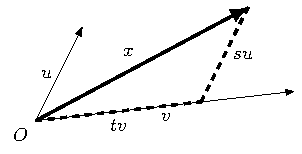
\includegraphics[width=0.5\textwidth]{figuras/generado-por-dos-vectores.pdf}
        \caption{El generado de $\{u,v\}$ es el plano que pasa por el origen, $u$ y $v$.}
    \end{figure}

    Usualmente existen muchos subconjuntos distintos que generan a un subespacio $W$. (Véase el Ejercicio~73.) Es natural buscar un subconjunto de $W$ que genere a $W$ y que sea tan pequeño como sea posible. En la siguiente sección exploramos las circunstancias bajo las cuales un vector puede eliminarse de un conjunto generador para obtener un conjunto generador más pequeño.

    \begin{ejercicio}
        Etiquete las siguientes afirmaciones como verdaderas o falsas.
        \begin{enumerate}[label=(\alph*)]
            \item El vector cero es una combinación lineal de cualquier conjunto no vacío de vectores.
            \item El generado de $\emptyset$ es $\emptyset$.
            \item Si $S$ es un subconjunto de un espacio vectorial $V$, entonces $\gen{S}$ es igual a la intersección de todos los subespacios de $V$ que contienen a $S$.
            \item Al resolver un sistema de ecuaciones lineales, es permisible multiplicar una ecuación por cualquier constante.
            \item Al resolver un sistema de ecuaciones lineales, es permisible sumar cualquier múltiplo de una ecuación a otra.
            \item Todo sistema de ecuaciones lineales tiene solución.
        \end{enumerate}
    \end{ejercicio}

    \begin{ejercicio}
        Resuelva los siguientes sistemas de ecuaciones lineales usando el método introducido en esta sección.
        \begin{enumerate}[label=(\alph*)]
            \item
            \begin{align*}
                2x_1-2x_2-3x_3&=-2\\
                3x_1-3x_2-2x_3+5x_4&=7\\
                x_1-x_2-2x_3-x_4&=-3
            \end{align*}
            \item
            \begin{align*}
                3x_1-7x_2+4x_3&=10\\
                x_1-2x_2+x_3&=3\\
                2x_1-x_2-2x_3&=6
            \end{align*}
            \item
            \begin{align*}
                x_1+2x_2-x_3+x_4&=5\\
                x_1+4x_2-3x_3-3x_4&=6\\
                2x_1+3x_2-x_3+4x_4&=8
            \end{align*}
            \item
            \begin{align*}
                x_1+2x_2+2x_3&=2\\
                x_1+8x_3+5x_4&=-6\\
                x_1+x_2+5x_3+5x_4&=3
            \end{align*}
            \item
            \begin{align*}
                x_1+2x_2-4x_3-x_4+x_5&=7\\
                -x_1+10x_3-3x_4-4x_5&=-16\\
                2x_1+5x_2-5x_3-4x_4-x_5&=2\\
                4x_1+11x_2-7x_3-10x_4-2x_5&=7
            \end{align*}
            \item
            \begin{align*}
                x_1+2x_2+6x_3&=-1\\
                2x_1+x_2+x_3&=8\\
                3x_1+x_2-x_3&=15\\
                x_1+3x_2+10x_3&=-5
            \end{align*}
        \end{enumerate}
    \end{ejercicio}

    \begin{ejercicio}
        Para cada una de las siguientes listas de vectores en $\R^3$, determine si el primer vector puede expresarse como combinación lineal de los otros dos.
        \begin{enumerate}[label=(\alph*)]
            \item $(-2,0,3)$, $(1,3,0)$, $(2,4,-1)$
            \item $(1,2,-3)$, $(-3,2,1)$, $(2,-1,-1)$
            \item $(3,4,1)$, $(1,-2,1)$, $(-2,-1,1)$
            \item $(2,-1,0)$, $(1,2,-3)$, $(1,-3,2)$
            \item $(5,1,-5)$, $(1,-2,-3)$, $(-2,3,-4)$
            \item $(-2,2,2)$, $(1,2,-1)$, $(-3,-3,3)$
        \end{enumerate}
    \end{ejercicio}

    \begin{ejercicio}
        Para cada una de las siguientes listas de polinomios en $P_3(\R)$, determine si el primer polinomio puede expresarse como combinación lineal de los otros dos.
        \begin{enumerate}[label=(\alph*)]
            \item $x^3-3x+5$, $x^3+2x^2-x+1$, $x^3+3x^2-1$
            \item $4x^3+2x^2-6$, $x^3-2x^2+4x+1$, $3x^3-6x^2+x+4$
            \item $-2x^3-11x^2+3x+2$, $x^3-2x^2+3x-1$, $2x^3+x^2+3x-2$
            \item $x^3+x^2+2x+13$, $2x^3-3x^2+4x+1$, $x^3-x^2+2x+3$
            \item $x^3-8x^2+4x$, $x^3-2x^2+3x-1$, $x^3-2x^2+3$
            \item $6x^3-3x^2+x+2$, $x^3-x^2+2x+3$, $2x^3-3x+1$
        \end{enumerate}
    \end{ejercicio}

    \begin{ejercicio}
        En cada inciso, determine si el vector dado está en el generado de $S$.
        \begin{enumerate}[label=(\alph*)]
            \item $(2,-1,1)$, $S=\{(1,0,2),(-1,1,1)\}$
            \item $(-1,2,1)$, $S=\{(1,0,2),(-1,1,1)\}$
            \item $(-1,1,1,2)$, $S=\{(1,0,1,-1),(0,1,1,1)\}$
            \item $(2,-1,1,-3)$, $S=\{(1,0,1,-1),(0,1,1,1)\}$
            \item $-x^3+2x^2+3x+3$, $S=\{x^3+x^2+x+1,\,x^2+x+1,\,x+1\}$
            \item $2x^3-x^2+x+3$, $S=\{x^3+x^2+x+1,\,x^2+x+1,\,x+1\}$
            \item $\begin{pmatrix}1&2\\-3&4\end{pmatrix}$, $S=\left\{\begin{pmatrix}1&0\\-1&0\end{pmatrix},\begin{pmatrix}0&1\\0&1\end{pmatrix},\begin{pmatrix}1&1\\0&0\end{pmatrix}\right\}$
            \item $\begin{pmatrix}1&0\\0&1\end{pmatrix}$, $S=\left\{\begin{pmatrix}1&0\\-1&0\end{pmatrix},\begin{pmatrix}0&1\\0&1\end{pmatrix},\begin{pmatrix}1&1\\0&0\end{pmatrix}\right\}$
        \end{enumerate}
    \end{ejercicio}

    \begin{ejercicio}
        Muestre que los vectores $(1,1,0)$, $(1,0,1)$, y $(0,1,1)$ generan a $F^3$.
    \end{ejercicio}

    \begin{ejercicio}
        En $F^n$, sea $e_j$ el vector cuya $j$-ésima coordenada es $1$ y cuyas demás coordenadas son $0$. Pruebe que $\{e_1,e_2,\dots,e_n\}$ genera a $F^n$.
    \end{ejercicio}

    \begin{ejercicio}
        Muestre que $P_n(F)$ es generado por $\{1,x,\dots,x^n\}$.
    \end{ejercicio}

    \begin{ejercicio}
        Muestre que las matrices
        \begin{equation*}
            \begin{pmatrix}1&0\\0&0\end{pmatrix}, \quad \begin{pmatrix}0&1\\0&0\end{pmatrix}, \quad \begin{pmatrix}0&0\\1&0\end{pmatrix}, \quad\text{y}\quad \begin{pmatrix}0&0\\0&1\end{pmatrix}
        \end{equation*}
        generan a $M_{2\times 2}(F)$.
    \end{ejercicio}

    \begin{ejercicio}
        Muestre que, si
        \begin{equation*}
            M_1=\begin{pmatrix}1&0\\0&0\end{pmatrix}, \quad M_2=\begin{pmatrix}0&0\\0&1\end{pmatrix}, \quad\text{y}\quad M_3=\begin{pmatrix}0&1\\1&0\end{pmatrix},
        \end{equation*}
        entonces el generado de $\{M_1,M_2,M_3\}$ es el conjunto de todas las matrices simétricas $2\times 2$.
    \end{ejercicio}

    \begin{ejercicio}
        Pruebe que $\gen{\{x\}}=\{ax:a\in F\}$ para cualquier vector $x$ de un espacio vectorial. Interprete geométricamente este resultado en $\R^3$.
    \end{ejercicio}

    \begin{ejercicio}
        Muestre que un subconjunto $W$ de un espacio vectorial $V$ es un subespacio de $V$ si y solo si $\gen{W}=W$.
    \end{ejercicio}

    \begin{ejercicio}
        Muestre que si $S_1$ y $S_2$ son subconjuntos de un espacio vectorial $V$ tales que $S_1\subseteq S_2$, entonces $\gen{S_1}\subseteq\gen{S_2}$. En particular, si $S_1\subseteq S_2$ y $\gen{S_1}=V$, deduzca que $\gen{S_2}=V$.
    \end{ejercicio}

    \begin{ejercicio}
        Muestre que si $S_1$ y $S_2$ son subconjuntos arbitrarios de un espacio vectorial $V$, entonces $\gen{S_1\cup S_2}=\gen{S_1}+\gen{S_2}$. (La suma de dos subconjuntos se definió en los ejercicios de la Sección~1.3.)
    \end{ejercicio}

    \begin{ejercicio}
        Sean $S_1$ y $S_2$ subconjuntos de un espacio vectorial $V$. Pruebe que $\gen{S_1\cap S_2}\subseteq\gen{S_1}\cap\gen{S_2}$. Dé un ejemplo en el que $\gen{S_1\cap S_2}$ y $\gen{S_1}\cap\gen{S_2}$ sean iguales, y uno en el que sean distintos.
    \end{ejercicio}

    \begin{ejercicio}
        Sea $V$ un espacio vectorial y $S$ un subconjunto de $V$ con la propiedad de que, siempre que $v_1,v_2,\dots,v_n\in S$ y $a_1v_1+a_2v_2+\cdots+a_nv_n=0$, se tiene $a_1=a_2=\cdots=a_n=0$. Pruebe que todo vector del generado de $S$ puede escribirse de manera \textit{única} como combinación lineal de vectores de $S$.
    \end{ejercicio}

    \begin{ejercicio}
        Sea $W$ un subespacio de un espacio vectorial $V$. ¿Bajo qué condiciones existen solo un número finito de subconjuntos distintos $S$ de $W$ tales que $S$ genera a $W$?
    \end{ejercicio}

    \section{Dependencia e independencia lineal}

    Supongamos que $V$ es un espacio vectorial sobre un campo infinito y que $W$ es un subespacio de $V$. A menos que $W$ sea el subespacio cero, $W$ es un conjunto infinito. Es deseable encontrar un subconjunto finito \textquotedblleft pequeño\textquotedblright\ $S$ que genere a $W$, porque entonces podemos describir cada vector de $W$ como combinación lineal del número finito de vectores de $S$. En efecto, cuanto más pequeño sea $S$, menos cálculos se requieren para representar vectores en $W$. Consideremos, por ejemplo, el subespacio $W$ de $\R^3$ generado por $S=\{u_1,u_2,u_3,u_4\}$, donde $u_1=(2,-1,4)$, $u_2=(1,-1,3)$, $u_3=(1,1,-1)$ y $u_4=(1,-2,-1)$. Intentemos encontrar un subconjunto propio de $S$ que también genere a $W$. La búsqueda está relacionada con la pregunta de si algún vector de $S$ es una combinación lineal de los otros vectores de $S$. Ahora $u_4$ es una combinación lineal de los otros vectores de $S$ si y solo si existen escalares $a_1,a_2$ y $a_3$ tales que
    \begin{equation*}
        u_4=a_1u_1+a_2u_2+a_3u_3,
    \end{equation*}
    es decir, si y solo si existen escalares $a_1,a_2$ y $a_3$ que satisfacen
    \begin{equation*}
        (1,-2,-1)=(2a_1+a_2+a_3,\,-a_1-a_2+a_3,\,4a_1+3a_2-a_3).
    \end{equation*}
    Así $u_4$ es una combinación lineal de $u_1,u_2$ y $u_3$ si y solo si el sistema de ecuaciones lineales
    \begin{align*}
        2a_1+a_2+a_3&=1\\
        -a_1-a_2+a_3&=-2\\
        4a_1+3a_2-a_3&=-1
    \end{align*}
    tiene solución. El lector debe verificar que dicha solución no existe. Esto no responde, sin embargo, a nuestra pregunta de si \textit{algún} vector de $S$ es una combinación lineal de los otros vectores de $S$. Puede mostrarse, de hecho, que $u_3$ es una combinación lineal de $u_1$, $u_2$ y $u_4$, a saber, $u_3=2u_1-3u_2+0u_4$.

    En el ejemplo anterior, verificar que algún vector de $S$ es combinación lineal de los otros vectores de $S$ podría requerir que resolvamos varios sistemas de ecuaciones lineales distintos antes de determinar cuál, si alguno, de $u_1,u_2,u_3$ y $u_4$ es combinación lineal de los otros. Al formular nuestra pregunta de otra manera, podemos ahorrarnos trabajo. Observemos que, como $u_3=2u_1-3u_2+0u_4$, tenemos
    \begin{equation*}
        -2u_1+3u_2+u_3-0u_4=0.
    \end{equation*}
    Es decir, como algún vector de $S$ es combinación lineal de los otros, el vector cero puede expresarse como combinación lineal de los vectores de $S$ usando coeficientes que no son todos cero. El recíproco de esta afirmación también es cierto: si el vector cero puede escribirse como combinación lineal de los vectores de $S$ en la que no todos los coeficientes son cero, entonces algún vector de $S$ es combinación lineal de los otros. Por ejemplo, en el ejemplo anterior, la ecuación $-2u_1+3u_2+u_3-0u_4=0$ puede resolverse para cualquier vector que tenga un coeficiente no nulo; así $u_1$, $u_2$ o $u_3$ (pero no $u_4$) puede escribirse como combinación lineal de los otros tres vectores. Así, en lugar de preguntar si algún vector de $S$ es combinación lineal de los otros vectores de $S$, es más eficiente preguntar si el vector cero puede expresarse como combinación lineal de los vectores de $S$ con coeficientes que no sean todos cero. Esta observación nos lleva a la siguiente definición.

    \begin{definicion}[Dependencia lineal]
        Un subconjunto $S$ de un espacio vectorial $V$ se llama \textbf{linealmente dependiente} si existe un número finito de vectores distintos $u_1,u_2,\dots,u_n$ en $S$ y escalares $a_1,a_2,\dots,a_n$, no todos cero, tales que
        \begin{equation*}
            a_1u_1+a_2u_2+\cdots+a_nu_n=0.
        \end{equation*}
        En este caso también decimos que los vectores de $S$ son \textbf{linealmente dependientes}.
    \end{definicion}

    Para cualesquiera vectores $u_1,u_2,\dots,u_n$, tenemos $a_1u_1+a_2u_2+\cdots+a_nu_n=0$ si $a_1=a_2=\cdots=a_n=0$. A esta la llamamos la \textbf{representación trivial} de $0$ como combinación lineal de $u_1,u_2,\dots,u_n$. Así, para que un conjunto sea linealmente dependiente, debe existir una representación no trivial de $0$ como combinación lineal de vectores del conjunto. En consecuencia, cualquier subconjunto de un espacio vectorial que contenga al vector cero es linealmente dependiente, pues $0=1\cdot 0$ es una representación no trivial de $0$ como combinación lineal de vectores del conjunto.

    \begin{ejemplo}
        Consideremos el conjunto
        \begin{equation*}
            S=\{(1,3,-4,2),\,(2,2,-4,0),\,(1,-3,2,-4),\,(-1,0,1,0)\}
        \end{equation*}
        en $\R^4$. Mostramos que $S$ es linealmente dependiente y luego expresamos uno de los vectores de $S$ como combinación lineal de los otros vectores de $S$. Para mostrar que $S$ es linealmente dependiente, debemos encontrar escalares $a_1,a_2,a_3$ y $a_4$, no todos cero, tales que
        \begin{equation*}
            a_1(1,3,-4,2)+a_2(2,2,-4,0)+a_3(1,-3,2,-4)+a_4(-1,0,1,0)=0.
        \end{equation*}
        Encontrar tales escalares equivale a encontrar una solución no nula del sistema de ecuaciones lineales
        \begin{align*}
            a_1+2a_2+a_3-a_4&=0\\
            3a_1+2a_2-3a_3&=0\\
            -4a_1-4a_2+2a_3+a_4&=0\\
            2a_1-4a_3&=0.
        \end{align*}
        Una solución es $a_1=4$, $a_2=-3$, $a_3=2$ y $a_4=0$. Así $S$ es un subconjunto linealmente dependiente de $\R^4$, y
        \begin{equation*}
            4(1,3,-4,2)-3(2,2,-4,0)+2(1,-3,2,-4)+0(-1,0,1,0)=0.
        \end{equation*}
    \end{ejemplo}

    \begin{ejemplo}
        En $M_{2\times 3}(\R)$, el conjunto
        \begin{equation*}
            \left\{\begin{pmatrix}1&-3&2\\-4&0&5\end{pmatrix},\begin{pmatrix}-3&7&4\\6&-2&-7\end{pmatrix},\begin{pmatrix}-2&3&11\\-1&-3&2\end{pmatrix}\right\}
        \end{equation*}
        es linealmente dependiente porque
        \begin{equation*}
            5\begin{pmatrix}1&-3&2\\-4&0&5\end{pmatrix}+3\begin{pmatrix}-3&7&4\\6&-2&-7\end{pmatrix}-2\begin{pmatrix}-2&3&11\\-1&-3&2\end{pmatrix}=\begin{pmatrix}0&0&0\\0&0&0\end{pmatrix}.
        \end{equation*}
    \end{ejemplo}

    \begin{definicion}[Independencia lineal]
        Un subconjunto $S$ de un espacio vectorial que no es linealmente dependiente se llama \textbf{linealmente independiente}. Como antes, también decimos que los vectores de $S$ son \textbf{linealmente independientes}.
    \end{definicion}

    Los siguientes hechos sobre conjuntos linealmente independientes son ciertos en cualquier espacio vectorial.
    \begin{enumerate}
        \item El conjunto vacío es linealmente independiente, pues los conjuntos linealmente dependientes deben ser no vacíos.
        \item Un conjunto que consiste de un solo vector no nulo es linealmente independiente. Pues si $\{u\}$ fuera linealmente dependiente, entonces $au=0$ para algún escalar no nulo $a$. Así
        \begin{equation*}
            u=a^{-1}(au)=a^{-1}0=0.
        \end{equation*}
        \item Un conjunto es linealmente independiente si y solo si las únicas representaciones de $0$ como combinaciones lineales de sus vectores son las representaciones triviales.
    \end{enumerate}

    La condición del inciso 3 proporciona un método útil para determinar si un conjunto finito es linealmente independiente. Esta técnica se ilustra en los ejemplos que siguen.

    \begin{ejemplo}
        Para probar que el conjunto
        \begin{equation*}
            S=\{(1,0,0,-1),\,(0,1,0,-1),\,(0,0,1,-1),\,(0,0,0,1)\}
        \end{equation*}
        es linealmente independiente, debemos mostrar que la única combinación lineal de vectores de $S$ que es igual al vector cero es aquella en la que todos los coeficientes son cero. Supongamos que $a_1,a_2,a_3$ y $a_4$ son escalares tales que
        \begin{equation*}
            a_1(1,0,0,-1)+a_2(0,1,0,-1)+a_3(0,0,1,-1)+a_4(0,0,0,1)=(0,0,0,0).
        \end{equation*}
        Igualando las coordenadas correspondientes de los vectores en los lados izquierdo y derecho de esta ecuación, obtenemos el siguiente sistema de ecuaciones lineales:
        \begin{align*}
            a_1&=0\\
            a_2&=0\\
            a_3&=0\\
            -a_1-a_2-a_3+a_4&=0.
        \end{align*}
        Claramente la única solución de este sistema es $a_1=a_2=a_3=a_4=0$, así que $S$ es linealmente independiente.
    \end{ejemplo}

    \begin{ejemplo}
        Para $k=0,1,\dots,n$, sea $p_k(x)=x^k+x^{k+1}+\cdots+x^n$. El conjunto
        \begin{equation*}
            \{p_0(x),p_1(x),\dots,p_n(x)\}
        \end{equation*}
        es linealmente independiente en $P_n(F)$. En efecto, si
        \begin{equation*}
            a_0p_0(x)+a_1p_1(x)+\cdots+a_np_n(x)=0
        \end{equation*}
        para algunos escalares $a_0,a_1,\dots,a_n$, entonces
        \begin{equation*}
            a_0+(a_0+a_1)x+(a_0+a_1+a_2)x^2+\cdots+(a_0+a_1+\cdots+a_n)x^n=0.
        \end{equation*}
        Igualando los coeficientes de $x^k$ en ambos lados de esta ecuación, para $k=0,1,2,\dots,n$, obtenemos
        \begin{align*}
            a_0&=0\\
            a_0+a_1&=0\\
            a_0+a_1+a_2&=0\\
            &\ \,\vdots\\
            a_0+a_1+a_2+\cdots+a_n&=0.
        \end{align*}
        Claramente la única solución de este sistema de ecuaciones lineales es $a_0=a_1=\cdots=a_n=0$.
    \end{ejemplo}

    Los siguientes resultados importantes son consecuencias inmediatas de las definiciones de dependencia e independencia lineal.

    \begin{teorema}
        Sea $V$ un espacio vectorial, y sea $S_1\subseteq S_2\subseteq V$. Si $S_1$ es linealmente dependiente, entonces $S_2$ es linealmente dependiente.
    \end{teorema}

    \begin{proof}
        Como $S_1$ es linealmente dependiente, existen vectores distintos $u_1,u_2,\dots,u_n\in S_1$ y escalares $a_1,a_2,\dots,a_n$, no todos cero, tales que $a_1u_1+a_2u_2+\cdots+a_nu_n=0$. Como $S_1\subseteq S_2$, los vectores $u_1,u_2,\dots,u_n$ también están en $S_2$; así esta misma relación no trivial muestra que $S_2$ es linealmente dependiente.
    \end{proof}

    \begin{corolario}
        Sea $V$ un espacio vectorial, y sea $S_1\subseteq S_2\subseteq V$. Si $S_2$ es linealmente independiente, entonces $S_1$ es linealmente independiente.
    \end{corolario}

    \begin{proof}
        Si $S_1$ fuera linealmente dependiente, entonces, por el teorema anterior, $S_2$ sería linealmente dependiente, contrario a la hipótesis. Por tanto $S_1$ es linealmente independiente.
    \end{proof}

    Antes, en esta sección, observamos que la pregunta de si $S$ es el conjunto generador más pequeño para su generado está relacionada con la pregunta de si algún vector de $S$ es una combinación lineal de los otros vectores de $S$. Así, la pregunta de si $S$ es el conjunto generador más pequeño para su generado está relacionada con la pregunta de si $S$ es linealmente dependiente. Para verlo, consideremos el subconjunto $S=\{u_1,u_2,u_3,u_4\}$ de $\R^3$, donde $u_1=(2,-1,4)$, $u_2=(1,-1,3)$, $u_3=(1,1,-1)$ y $u_4=(1,-2,-1)$. Hemos observado antes que $S$ es linealmente dependiente; de hecho,
    \begin{equation*}
        -2u_1+3u_2+u_3-0u_4=0.
    \end{equation*}
    Esta ecuación implica que $u_3$ (o, alternativamente, $u_1$ o $u_2$) es una combinación lineal de los otros vectores de $S$. Por ejemplo, $u_3=2u_1-3u_2+0u_4$. Por tanto toda combinación lineal $a_1u_1+a_2u_2+a_3u_3+a_4u_4$ de vectores de $S$ puede escribirse como combinación lineal de $u_1,u_2$ y $u_4$:
    \begin{align*}
        a_1u_1+a_2u_2+a_3u_3+a_4u_4&=a_1u_1+a_2u_2+a_3(2u_1-3u_2+0u_4)+a_4u_4\\
        &=(a_1+2a_3)u_1+(a_2-3a_3)u_2+a_4u_4.
    \end{align*}
    Así el subconjunto $S'=\{u_1,u_2,u_4\}$ de $S$ tiene el mismo generado que $S$.

    Más generalmente, supongamos que $S$ es cualquier conjunto linealmente dependiente que contiene dos o más vectores. Entonces algún vector $v\in S$ puede escribirse como combinación lineal de los otros vectores de $S$, y el subconjunto que se obtiene al eliminar $v$ de $S$ tiene el mismo generado que $S$. Se sigue que \textit{si ningún subconjunto propio de $S$ genera el generado de $S$, entonces $S$ debe ser linealmente dependiente}. Otra forma de ver esta afirmación se da en el Teorema~1.7.

    \begin{teorema}
        Sea $S$ un subconjunto linealmente independiente de un espacio vectorial $V$, y sea $v$ un vector de $V$ que no está en $S$. Entonces $S\cup\{v\}$ es linealmente dependiente si y solo si $v\in\gen{S}$.
    \end{teorema}

    \begin{proof}
        Si $S\cup\{v\}$ es linealmente dependiente, entonces existen vectores $u_1,u_2,\dots,u_n$ en $S\cup\{v\}$ tales que $a_1u_1+a_2u_2+\cdots+a_nu_n=0$ para algunos escalares $a_1,a_2,\dots,a_n$, no todos cero. Como $S$ es linealmente independiente, uno de los $u_i$, digamos $u_1$, es igual a $v$. Así
        \begin{equation*}
            a_1v+a_2u_2+\cdots+a_nu_n=0,
        \end{equation*}
        y
        \begin{equation*}
            v=a_1^{-1}(-a_2u_2-\cdots-a_nu_n)=(-a_1^{-1}a_2)u_2-\cdots-(a_1^{-1}a_n)u_n.
        \end{equation*}
        (Notemos que $a_1\neq 0$, pues, si $a_1=0$, la relación $a_1v+a_2u_2+\cdots+a_nu_n=0$ sería una relación de dependencia lineal no trivial entre vectores de $S$, contradiciendo la independencia lineal de $S$.) Como $v$ es una combinación lineal de $u_2,\dots,u_n$, los cuales están en $S$, tenemos $v\in\gen{S}$.

        Recíprocamente, sea $v\in\gen{S}$. Entonces existen vectores $v_1,v_2,\dots,v_m$ en $S$ y escalares $b_1,b_2,\dots,b_m$ tales que $v=b_1v_1+b_2v_2+\cdots+b_mv_m$. De aquí,
        \begin{equation*}
            0=b_1v_1+b_2v_2+\cdots+b_mv_m+(-1)v.
        \end{equation*}
        Como $v\neq v_i$ para $i=1,2,\dots,m$, el coeficiente de $v$ en esta combinación lineal es no nulo, y así el conjunto $\{v_1,v_2,\dots,v_m,v\}$ es linealmente dependiente. Por tanto $S\cup\{v\}$ es linealmente dependiente por el teorema anterior.
    \end{proof}

    Los conjuntos generadores linealmente independientes se investigan en detalle en la Sección~1.6.

    \begin{ejercicio}
        Etiquete las siguientes afirmaciones como verdaderas o falsas.
        \begin{enumerate}[label=(\alph*)]
            \item Si $S$ es un conjunto linealmente dependiente, entonces cada vector de $S$ es combinación lineal de otros vectores de $S$.
            \item Cualquier conjunto que contenga al vector cero es linealmente dependiente.
            \item El conjunto vacío es linealmente dependiente.
            \item Los subconjuntos de conjuntos linealmente dependientes son linealmente dependientes.
            \item Los subconjuntos de conjuntos linealmente independientes son linealmente independientes.
            \item Si $a_1x_1+a_2x_2+\cdots+a_nx_n=0$ y $x_1,x_2,\dots,x_n$ son linealmente independientes, entonces todos los escalares $a_i$ son cero.
        \end{enumerate}
    \end{ejercicio}

    \begin{ejercicio}
        Determine si los siguientes conjuntos son linealmente dependientes o linealmente independientes.\footnote{Los cálculos de los incisos (g), (h), (i) y (j) son tediosos a menos que se use tecnología.}
        \begin{enumerate}[label=(\alph*)]
            \item $\left\{\begin{pmatrix}1&-3\\-2&4\end{pmatrix},\begin{pmatrix}-2&6\\4&-8\end{pmatrix}\right\}$ en $M_{2\times 2}(\R)$
            \item $\left\{\begin{pmatrix}1&-2\\-1&4\end{pmatrix},\begin{pmatrix}-1&1\\2&-4\end{pmatrix}\right\}$ en $M_{2\times 2}(\R)$
            \item $\{x^3+2x^2,\,-x^2+3x+1,\,x^3-x^2+2x-1\}$ en $P_3(\R)$
            \item $\{x^3-x,\,2x^2+4,\,-2x^3+3x^2+2x+6\}$ en $P_3(\R)$
            \item $\{(1,-1,2),(1,-2,1),(1,1,4)\}$ en $\R^3$
            \item $\{(1,-1,2),(2,0,1),(-1,2,-1)\}$ en $\R^3$
            \item $\left\{\begin{pmatrix}1&0\\-2&1\end{pmatrix},\begin{pmatrix}0&-1\\1&1\end{pmatrix},\begin{pmatrix}-1&2\\1&0\end{pmatrix},\begin{pmatrix}2&1\\-4&4\end{pmatrix}\right\}$ en $M_{2\times 2}(\R)$
            \item $\left\{\begin{pmatrix}1&0\\-2&1\end{pmatrix},\begin{pmatrix}0&-1\\1&1\end{pmatrix},\begin{pmatrix}-1&2\\1&0\end{pmatrix},\begin{pmatrix}2&1\\2&-2\end{pmatrix}\right\}$ en $M_{2\times 2}(\R)$
            \item $\{x^4-x^3+5x^2-8x+6,\,-x^4+x^3-5x^2+5x-3,\,x^4+3x^2-3x+5,\,2x^4+3x^3+4x^2-x+2,\,x^3-x+2\}$ en $P_4(\R)$
            \item $\{x^4-x^3+5x^2-8x+6,\,-x^4+x^3-5x^2+5x-3,\,x^4+3x^2-3x+5,\,2x^4+x^3+4x^2+8x\}$ en $P_4(\R)$
        \end{enumerate}
    \end{ejercicio}

    \begin{ejercicio}
        En $M_{2\times 3}(F)$, pruebe que el conjunto
        \begin{equation*}
            \left\{\begin{pmatrix}1&1&0\\0&0&0\end{pmatrix},\begin{pmatrix}0&0&1\\1&0&0\end{pmatrix},\begin{pmatrix}0&0&0\\0&1&1\end{pmatrix},\begin{pmatrix}1&0&1\\1&0&0\end{pmatrix},\begin{pmatrix}0&1&0\\0&1&1\end{pmatrix}\right\}
        \end{equation*}
        es linealmente dependiente.
    \end{ejercicio}

    \begin{ejercicio}
        En $F^n$, sea $e_j$ el vector cuya $j$-ésima coordenada es $1$ y cuyas demás coordenadas son $0$. Pruebe que $\{e_1,e_2,\dots,e_n\}$ es linealmente independiente.
    \end{ejercicio}

    \begin{ejercicio}
        Muestre que el conjunto $\{1,x,x^2,\dots,x^n\}$ es linealmente independiente en $P_n(F)$.
    \end{ejercicio}

    \begin{ejercicio}
        En $M_{m\times n}(F)$, sea $E^{ij}$ la matriz cuya única entrada no nula es un $1$ en el renglón $i$ y la columna $j$. Pruebe que $\{E^{ij}:1\leq i\leq m,\,1\leq j\leq n\}$ es linealmente independiente.
    \end{ejercicio}

    \begin{ejercicio}
        Recordemos, del Ejemplo~12 de la Sección~1.3, que el conjunto de las matrices diagonales en $M_{2\times 2}(F)$ es un subespacio. Encuentre un conjunto linealmente independiente que genere este subespacio.
    \end{ejercicio}

    \begin{ejercicio}
        Sea $S=\{(1,1,0),(1,0,1),(0,1,1)\}$ un subconjunto del espacio vectorial $F^3$.
        \begin{enumerate}[label=(\alph*)]
            \item Pruebe que, si $F=\R$, entonces $S$ es linealmente independiente.
            \item Pruebe que, si $F$ tiene característica $2$, entonces $S$ es linealmente dependiente.
        \end{enumerate}
    \end{ejercicio}

    \begin{ejercicio}
        Sean $u$ y $v$ vectores distintos de un espacio vectorial $V$. Muestre que $\{u,v\}$ es linealmente dependiente si y solo si $u$ o $v$ es un múltiplo del otro.
    \end{ejercicio}

    \begin{ejercicio}
        Dé un ejemplo de tres vectores linealmente dependientes en $\R^3$ tales que ninguno de los tres sea múltiplo de otro.
    \end{ejercicio}

    \begin{ejercicio}
        Sea $S=\{u_1,u_2,\dots,u_n\}$ un subconjunto linealmente independiente de un espacio vectorial $V$ sobre el campo $\Z_2$. ¿Cuántos vectores hay en $\gen{S}$? Justifique su respuesta.
    \end{ejercicio}

    \begin{ejercicio}
        Pruebe el Teorema~1.6 y su corolario.
    \end{ejercicio}

    \begin{ejercicio}
        Sea $V$ un espacio vectorial sobre un campo de característica distinta de $2$.
        \begin{enumerate}[label=(\alph*)]
            \item Sean $u$ y $v$ vectores distintos de $V$. Pruebe que $\{u,v\}$ es linealmente independiente si y solo si $\{u+v,u-v\}$ es linealmente independiente.
            \item Sean $u$, $v$ y $w$ vectores distintos de $V$. Pruebe que $\{u,v,w\}$ es linealmente independiente si y solo si $\{u+v,u+w,v+w\}$ es linealmente independiente.
        \end{enumerate}
    \end{ejercicio}

    \begin{ejercicio}
        Pruebe que un conjunto $S$ es linealmente dependiente si y solo si $S=\{0\}$ o existen vectores distintos $v,u_1,u_2,\dots,u_n$ en $S$ tales que $v$ es combinación lineal de $u_1,u_2,\dots,u_n$.
    \end{ejercicio}

    \begin{ejercicio}
        Sea $S=\{u_1,u_2,\dots,u_n\}$ un conjunto finito de vectores. Pruebe que $S$ es linealmente dependiente si y solo si $u_1=0$ o $u_{k+1}\in\gen{\{u_1,u_2,\dots,u_k\}}$ para algún $k$ con $1\leq k<n$.
    \end{ejercicio}

    \begin{ejercicio}
        Pruebe que un conjunto $S$ de vectores es linealmente independiente si y solo si cada subconjunto finito de $S$ es linealmente independiente.
    \end{ejercicio}

    \begin{ejercicio}
        Sea $M$ una matriz cuadrada triangular superior (como se definió en el Ejercicio~41 de la Sección~1.3) con entradas diagonales no nulas. Pruebe que las columnas de $M$ son linealmente independientes.
    \end{ejercicio}

    \begin{ejercicio}
        Sea $S$ un conjunto de polinomios no nulos en $P(F)$ tales que dos cualesquiera de ellos tienen grados distintos. Pruebe que $S$ es linealmente independiente.
    \end{ejercicio}

    \begin{ejercicio}
        Pruebe que si $\{A_1,A_2,\dots,A_k\}$ es un subconjunto linealmente independiente de $M_{n\times n}(F)$, entonces $\{A_1^t,A_2^t,\dots,A_k^t\}$ también es linealmente independiente.
    \end{ejercicio}

    \begin{ejercicio}
        Sean $f,g\in\mathcal{F}(\R,\R)$ las funciones definidas por $f(t)=e^{rt}$ y $g(t)=e^{st}$, donde $r\neq s$. Pruebe que $f$ y $g$ son linealmente independientes en $\mathcal{F}(\R,\R)$.
    \end{ejercicio}

    \section{Bases y dimensión}

    \begin{definicion}[Base]
        Una \textbf{base} $\BB$ para un espacio vectorial $V$ es un subconjunto linealmente independiente de $V$ que genera a $V$. Si $\BB$ es una base para $V$, también decimos que los vectores de $\BB$ forman una base para $V$.
    \end{definicion}

    \begin{ejemplo}
        Recordando que $\gen{\emptyset}=\{0\}$ y que $\emptyset$ es linealmente independiente, vemos que $\emptyset$ es una base para el espacio vectorial cero.
    \end{ejemplo}

    \begin{ejemplo}
        En $F^n$, sean $e_1=(1,0,0,\dots,0)$, $e_2=(0,1,0,\dots,0)$, $\dots$, $e_n=(0,0,\dots,0,1)$; es fácil ver que $\{e_1,e_2,\dots,e_n\}$ es una base para $F^n$, llamada la \textbf{base canónica} (o \textbf{estándar}) para $F^n$.
    \end{ejemplo}

    \begin{ejemplo}
        En $M_{m\times n}(F)$, sea $E^{ij}$ la matriz cuya única entrada no nula es un $1$ en el renglón $i$ y la columna $j$. Entonces $\{E^{ij}:1\leq i\leq m,\,1\leq j\leq n\}$ es una base para $M_{m\times n}(F)$.
    \end{ejemplo}

    \begin{ejemplo}
        En $P_n(F)$, el conjunto $\{1,x,x^2,\dots,x^n\}$ es una base, llamada la \textbf{base canónica} (o \textbf{estándar}) para $P_n(F)$.
    \end{ejemplo}

    \begin{ejemplo}
        En $P(F)$, el conjunto $\{1,x,x^2,\dots\}$ es una base.
    \end{ejemplo}

    Observemos que el ejemplo anterior muestra que una base no necesita ser finita. De hecho, más adelante en esta sección se muestra que ninguna base para $P(F)$ puede ser finita. Por tanto no todo espacio vectorial tiene una base finita.

    El siguiente teorema, que se usa con frecuencia en el Capítulo~2, establece la propiedad más significativa de una base.

    \begin{teorema}
        Sea $V$ un espacio vectorial y $\BB=\{u_1,u_2,\dots,u_n\}$ un subconjunto de $V$. Entonces $\BB$ es una base para $V$ si y solo si cada $v\in V$ puede expresarse de manera \textit{única} como combinación lineal de los vectores de $\BB$, es decir, puede expresarse en la forma
        \begin{equation*}
            v=a_1u_1+a_2u_2+\cdots+a_nu_n
        \end{equation*}
        para escalares únicos $a_1,a_2,\dots,a_n$.
    \end{teorema}

    \begin{proof}
        Sea $\BB$ una base para $V$. Si $v\in V$, entonces $v\in\gen{\BB}$ porque $\gen{\BB}=V$. Así $v$ es una combinación lineal de los vectores de $\BB$. Supongamos que
        \begin{equation*}
            v=a_1u_1+a_2u_2+\cdots+a_nu_n \qquad\text{y}\qquad v=b_1u_1+b_2u_2+\cdots+b_nu_n
        \end{equation*}
        son dos representaciones de $v$ de este tipo. Restando la segunda ecuación de la primera se obtiene
        \begin{equation*}
            0=(a_1-b_1)u_1+(a_2-b_2)u_2+\cdots+(a_n-b_n)u_n.
        \end{equation*}
        Como $\BB$ es linealmente independiente, se sigue que $a_1-b_1=a_2-b_2=\cdots=a_n-b_n=0$. Así $a_1=b_1,a_2=b_2,\dots,a_n=b_n$, y $v$ se expresa de manera única como combinación lineal de los vectores de $\BB$.

        Recíprocamente, supongamos que cada $v\in V$ puede expresarse de manera única como combinación lineal de los vectores de $\BB$. Claramente esto implica que $V=\gen{\BB}$. Además, si
        \begin{equation*}
            0=a_1u_1+a_2u_2+\cdots+a_nu_n
        \end{equation*}
        para algunos escalares $a_1,a_2,\dots,a_n$, entonces, como $0=0u_1+0u_2+\cdots+0u_n$ es también una representación de $0$ como combinación lineal de los vectores de $\BB$, la unicidad de la representación implica que $a_1=a_2=\cdots=a_n=0$. Por tanto $\BB$ es linealmente independiente, y así $\BB$ es una base para $V$.
    \end{proof}

    El Teorema~1.8 muestra que, si los vectores $u_1,u_2,\dots,u_n$ forman una base para un espacio vectorial $V$, entonces todo vector en $V$ puede expresarse de manera única en la forma
    \begin{equation*}
        v=a_1u_1+a_2u_2+\cdots+a_nu_n
    \end{equation*}
    para escalares $a_1,a_2,\dots,a_n$ elegidos apropiadamente. Así $v$ determina una $n$-ada única de escalares $(a_1,a_2,\dots,a_n)$ y, recíprocamente, cada $n$-ada de escalares determina un único vector $v\in V$ usando las entradas de la $n$-ada como los coeficientes de una combinación lineal de $u_1,u_2,\dots,u_n$. Este hecho sugiere que $V$ es semejante al espacio vectorial $F^n$, donde $n$ es el número de vectores en la base para $V$. Veremos en la Sección~2.4 que esto efectivamente es así.

    En este libro nos interesan principalmente los espacios vectoriales que tienen bases finitas. El Teorema~1.9 identifica una amplia clase de espacios vectoriales de este tipo.

    \begin{teorema}
        Si un espacio vectorial $V$ es generado por un conjunto finito $S$, entonces algún subconjunto de $S$ es una base para $V$. Por tanto $V$ tiene una base finita.
    \end{teorema}

    \begin{proof}
        Si $S=\emptyset$ o $S=\{0\}$, entonces $V=\{0\}$ y $\emptyset$ es una base para $V$. En caso contrario, $S$ contiene un vector no nulo $u_1$. Por el punto 2 de la Sección~1.5, $\{u_1\}$ es un conjunto linealmente independiente. Continuamos, si es posible, eligiendo vectores $u_2,\dots,u_k$ en $S$ tales que $\{u_1,u_2,\dots,u_k\}$ sea linealmente independiente. Como $S$ es un conjunto finito, eventualmente debemos llegar a una etapa en la cual $\BB=\{u_1,u_2,\dots,u_k\}$ es linealmente independiente, pero al agregar a $\BB$ cualquier vector de $S$ que no esté en $\BB$ se produce un conjunto linealmente dependiente. Afirmamos que $\BB$ es una base para $V$. Como $\BB$ es linealmente independiente por construcción, basta mostrar que $\BB$ genera a $V$. Por el Teorema~1.5, necesitamos mostrar que $S\subseteq\gen{\BB}$. Sea $v\in S$. Si $v\in\BB$, claramente $v\in\gen{\BB}$. En caso contrario, si $v\notin\BB$, entonces, por la construcción anterior, $\BB\cup\{v\}$ es linealmente dependiente. Así $v\in\gen{\BB}$ por el Teorema~1.7. Por tanto $S\subseteq\gen{\BB}$.
    \end{proof}

    Debido al método por el cual se obtuvo la base $\BB$ en la demostración del Teorema~1.9, este teorema se recuerda frecuentemente diciendo que \textit{un conjunto generador finito para $V$ puede reducirse a una base para $V$}. Este método se ilustra en el siguiente ejemplo.

    \begin{ejemplo}
        Sea
        \begin{equation*}
            S=\{(2,-3,5),(8,-12,20),(1,0,-2),(0,2,-1),(7,2,0)\}.
        \end{equation*}
        Puede mostrarse que $S$ genera a $\R^3$. Podemos seleccionar una base para $\R^3$ que sea un subconjunto de $S$ mediante la técnica usada en la demostración del Teorema~1.9. Para empezar, elegimos cualquier vector no nulo de $S$, digamos $(2,-3,5)$, como vector de la base. Como $4(2,-3,5)=(8,-12,20)$, el conjunto $\{(2,-3,5),(8,-12,20)\}$ es linealmente dependiente por el Ejercicio~86 de la Sección~1.5. Por tanto no incluimos $(8,-12,20)$ en nuestra base. Por otro lado, $(1,0,-2)$ no es múltiplo de $(2,-3,5)$ y viceversa, así que el conjunto $\{(2,-3,5),(1,0,-2)\}$ es linealmente independiente. Así incluimos $(1,0,-2)$ como parte de nuestra base.

        Consideramos ahora el conjunto $\{(2,-3,5),(1,0,-2),(0,2,-1)\}$ obtenido al agregar otro vector de $S$ a los dos que ya hemos incluido en nuestra base. Como antes, incluimos $(0,2,-1)$ en nuestra base o lo excluimos, según si $\{(2,-3,5),(1,0,-2),(0,2,-1)\}$ es linealmente independiente o linealmente dependiente. Un cálculo sencillo muestra que este conjunto es linealmente independiente, así que incluimos $(0,2,-1)$ en nuestra base. De manera similar, el último vector de $S$ se incluye o se excluye de nuestra base según si el conjunto
        \begin{equation*}
            \{(2,-3,5),(1,0,-2),(0,2,-1),(7,2,0)\}
        \end{equation*}
        es linealmente independiente o linealmente dependiente. Como
        \begin{equation*}
            2(2,-3,5)+3(1,0,-2)+4(0,2,-1)-(7,2,0)=(0,0,0),
        \end{equation*}
        excluimos $(7,2,0)$ de nuestra base. Concluimos que
        \begin{equation*}
            \{(2,-3,5),(1,0,-2),(0,2,-1)\}
        \end{equation*}
        es un subconjunto de $S$ que es una base para $\R^3$.
    \end{ejemplo}

    Los corolarios del siguiente teorema son, quizás, los resultados más significativos de este capítulo.

    \begin{teorema}[Teorema de reemplazo]
        Sea $V$ un espacio vectorial generado por un conjunto $G$ que contiene exactamente $n$ vectores, y sea $L$ un subconjunto linealmente independiente de $V$ que contiene exactamente $m$ vectores. Entonces $m\leq n$ y existe un subconjunto $H$ de $G$ que contiene exactamente $n-m$ vectores tal que $L\cup H$ genera a $V$.
    \end{teorema}

    \begin{proof}
        La demostración es por inducción matemática sobre $m$. La inducción comienza con $m=0$; en este caso $L=\emptyset$, y así, tomando $H=G$, se obtiene el resultado deseado.

        Supongamos ahora que el teorema es válido para algún entero $m\geq 0$. Probamos que el teorema es válido para $m+1$. Sea $L=\{v_1,v_2,\dots,v_{m+1}\}$ un subconjunto linealmente independiente de $V$ que consiste de $m+1$ vectores. Por el corolario al Teorema~1.6, $\{v_1,v_2,\dots,v_m\}$ es linealmente independiente, así que podemos aplicar la hipótesis de inducción para concluir que $m\leq n$ y que existe un subconjunto $\{u_1,u_2,\dots,u_{n-m}\}$ de $G$ tal que $\{v_1,v_2,\dots,v_m\}\cup\{u_1,u_2,\dots,u_{n-m}\}$ genera a $V$. Así existen escalares $a_1,a_2,\dots,a_m,b_1,b_2,\dots,b_{n-m}$ tales que
        \begin{equation*}
            a_1v_1+a_2v_2+\cdots+a_mv_m+b_1u_1+b_2u_2+\cdots+b_{n-m}u_{n-m}=v_{m+1}. \tag{9}
        \end{equation*}
        Notemos que, si $n-m=0$, el lado izquierdo de (9) es una combinación lineal de $v_1,v_2,\dots,v_m$, lo cual, por el Teorema~1.7, contradice la suposición de que $L$ es linealmente independiente. Por tanto $n>m$; es decir, $n\geq m+1$. Más aún, algún $b_i$, digamos $b_1$, es no nulo, pues de otro modo obtenemos la misma contradicción. Resolviendo (9) para $u_1$ se obtiene
        \begin{equation*}
            u_1=(-b_1^{-1}a_1)v_1+(-b_1^{-1}a_2)v_2+\cdots+(-b_1^{-1}a_m)v_m+(b_1^{-1})v_{m+1}+(-b_1^{-1}b_2)u_2+\cdots+(-b_1^{-1}b_{n-m})u_{n-m}.
        \end{equation*}
        Sea $H=\{u_2,\dots,u_{n-m}\}$. Entonces $u_1\in\gen{L\cup H}$, y, como $v_1,v_2,\dots,v_m,u_2,\dots,u_{n-m}$ están claramente en $\gen{L\cup H}$, se sigue que
        \begin{equation*}
            \{v_1,v_2,\dots,v_m,u_1,u_2,\dots,u_{n-m}\}\subseteq\gen{L\cup H}.
        \end{equation*}
        Como $\{v_1,v_2,\dots,v_m,u_1,u_2,\dots,u_{n-m}\}$ genera a $V$, el Teorema~1.5 implica que $\gen{L\cup H}=V$. Como $H$ es un subconjunto de $G$ que contiene $(n-m)-1=n-(m+1)$ vectores, el teorema es válido para $m+1$. Esto completa la inducción.
    \end{proof}

    \begin{corolario}
        Sea $V$ un espacio vectorial que tiene una base finita. Entonces toda base para $V$ contiene el mismo número de vectores.
    \end{corolario}

    \begin{proof}
        Supongamos que $\BB$ es una base finita para $V$ que contiene exactamente $n$ vectores, y sea $\gamma$ cualquier otra base para $V$. Si $\gamma$ contiene más de $n$ vectores, entonces podemos seleccionar un subconjunto $S$ de $\gamma$ que contenga exactamente $n+1$ vectores. Como $S$ es linealmente independiente y $\BB$ genera a $V$, el teorema de reemplazo implica que $n+1\leq n$, una contradicción. Por tanto $\gamma$ es finito, y el número $m$ de vectores en $\gamma$ satisface $m\leq n$. Invirtiendo los papeles de $\BB$ y $\gamma$ y argumentando de manera análoga, obtenemos $n\leq m$. Por tanto $m=n$.
    \end{proof}

    Si un espacio vectorial tiene una base finita, el Corolario~1 afirma que el número de vectores en \textit{cualquier} base para $V$ es una propiedad intrínseca de $V$. Este hecho hace posibles las siguientes definiciones importantes.

    \begin{definicion}[Dimensión]
        Un espacio vectorial se llama \textbf{de dimensión finita} si tiene una base que consiste de un número finito de vectores. El número único de vectores en cada base para $V$ se llama la \textbf{dimensión} de $V$ y se denota $\dim(V)$. Un espacio vectorial que no es de dimensión finita se llama \textbf{de dimensión infinita}.
    \end{definicion}

    Los siguientes resultados son consecuencias de los Ejemplos 1 al 4.

    \begin{ejemplo}
        El espacio vectorial $\{0\}$ tiene dimensión cero.
    \end{ejemplo}

    \begin{ejemplo}
        El espacio vectorial $F^n$ tiene dimensión $n$.
    \end{ejemplo}

    \begin{ejemplo}
        El espacio vectorial $M_{m\times n}(F)$ tiene dimensión $mn$.
    \end{ejemplo}

    \begin{ejemplo}
        El espacio vectorial $P_n(F)$ tiene dimensión $n+1$.
    \end{ejemplo}

    Los siguientes ejemplos muestran que la dimensión de un espacio vectorial depende de su campo de escalares.

    \begin{ejemplo}
        Sobre el campo de los números complejos, el espacio vectorial de los números complejos tiene dimensión $1$. (Una base es $\{1\}$.)
    \end{ejemplo}

    \begin{ejemplo}
        Sobre el campo de los números reales, el espacio vectorial de los números complejos tiene dimensión $2$. (Una base es $\{1,i\}$.)
    \end{ejemplo}

    En la terminología de la dimensión, la primera conclusión del teorema de reemplazo establece que, si $V$ es un espacio vectorial de dimensión finita, entonces ningún subconjunto linealmente independiente de $V$ puede contener más de $\dim(V)$ vectores. De este hecho se sigue que el espacio vectorial $P(F)$ es de dimensión infinita, porque tiene un conjunto linealmente independiente infinito, a saber $\{1,x,x^2,\dots\}$. Este conjunto es, de hecho, una base para $P(F)$. Sin embargo, nada de lo que hemos probado en esta sección garantiza que un espacio vectorial de dimensión infinita deba tener una base. En la Sección~1.7 se muestra, no obstante, que \textit{todo} espacio vectorial tiene una base.

    Así como ningún subconjunto linealmente independiente de un espacio vectorial de dimensión finita $V$ puede contener más de $\dim(V)$ vectores, puede hacerse una afirmación correspondiente sobre el tamaño de un conjunto generador.

    \begin{corolario}
        Sea $V$ un espacio vectorial con dimensión $n$.
        \begin{enumerate}[label=(\alph*)]
            \item Cualquier conjunto generador finito para $V$ contiene al menos $n$ vectores, y un conjunto generador para $V$ que contiene exactamente $n$ vectores es una base para $V$.
            \item Cualquier subconjunto linealmente independiente de $V$ que contiene exactamente $n$ vectores es una base para $V$.
            \item Todo subconjunto linealmente independiente de $V$ puede extenderse a una base para $V$.
        \end{enumerate}
    \end{corolario}

    \begin{proof}
        Sea $\BB$ una base para $V$.

        (a) Sea $G$ un conjunto generador finito para $V$. Por el Teorema~1.9, algún subconjunto $H$ de $G$ es una base para $V$. El Corolario~1 implica que $H$ contiene exactamente $n$ vectores. Como un subconjunto de $G$ contiene $n$ vectores, $G$ debe contener al menos $n$ vectores. Más aún, si $G$ contiene exactamente $n$ vectores, entonces debemos tener $H=G$, de modo que $G$ es una base para $V$.

        (b) Sea $L$ un subconjunto linealmente independiente de $V$ que contiene exactamente $n$ vectores. Se sigue del teorema de reemplazo que existe un subconjunto $H$ de $\BB$ que contiene $n-n=0$ vectores tal que $L\cup H$ genera a $V$. Así $H=\emptyset$, y $L$ genera a $V$. Como $L$ es también linealmente independiente, $L$ es una base para $V$.

        (c) Si $L$ es un subconjunto linealmente independiente de $V$ que contiene $m$ vectores, el teorema de reemplazo asegura que existe un subconjunto $H$ de $\BB$ que contiene exactamente $n-m$ vectores tal que $L\cup H$ genera a $V$. Ahora $L\cup H$ contiene a lo más $n$ vectores; por tanto (a) implica que $L\cup H$ contiene exactamente $n$ vectores y que $L\cup H$ es una base para $V$.
    \end{proof}

    \begin{ejemplo}
        Se sigue del Ejemplo~18 de la Sección~1.4 y del inciso (a) del corolario anterior que
        \begin{equation*}
            \{x^2+3x-2,\,2x^2+5x-3,\,-x^2-4x+4\}
        \end{equation*}
        es una base para $P_2(\R)$.
    \end{ejemplo}

    \begin{ejemplo}
        Se sigue del Ejemplo~19 de la Sección~1.4 y del inciso (a) del corolario anterior que
        \begin{equation*}
            \left\{\begin{pmatrix}1&1\\1&0\end{pmatrix},\begin{pmatrix}1&1\\0&1\end{pmatrix},\begin{pmatrix}1&0\\1&1\end{pmatrix},\begin{pmatrix}0&1\\1&1\end{pmatrix}\right\}
        \end{equation*}
        es una base para $M_{2\times 2}(\R)$.
    \end{ejemplo}

    \begin{ejemplo}
        Se sigue del Ejemplo~22 de la Sección~1.5 y del inciso (b) del corolario anterior que
        \begin{equation*}
            \{(1,0,0,-1),(0,1,0,-1),(0,0,1,-1),(0,0,0,1)\}
        \end{equation*}
        es una base para $\R^4$.
    \end{ejemplo}

    \begin{ejemplo}
        Para $k=0,1,\dots,n$, sea $p_k(x)=x^k+x^{k+1}+\cdots+x^n$. Se sigue del Ejemplo~23 de la Sección~1.5 y del inciso (b) del corolario anterior que
        \begin{equation*}
            \{p_0(x),p_1(x),\dots,p_n(x)\}
        \end{equation*}
        es una base para $P_n(F)$.
    \end{ejemplo}

    Un procedimiento para reducir un conjunto generador a una base se ilustró en el ejemplo del vector $(2,-3,5)$, etc., de esta sección. En la Sección~3.4, cuando hayamos aprendido más sobre resolver sistemas de ecuaciones lineales, descubriremos un método más sencillo para reducir un conjunto generador a una base. Este procedimiento también puede usarse para extender un conjunto linealmente independiente a una base, como afirma el inciso (c) del corolario anterior.

    \subsection*{Panorama general de la dimensión y sus consecuencias}

    El Teorema~1.9, así como el teorema de reemplazo y sus corolarios, contienen una gran cantidad de información sobre las relaciones entre conjuntos linealmente independientes, bases y conjuntos generadores. Por esta razón, resumimos aquí los principales resultados de esta sección para ponerlos en mejor perspectiva.

    Una base para un espacio vectorial $V$ es un subconjunto linealmente independiente de $V$ que genera a $V$. Si $V$ tiene una base finita, entonces toda base para $V$ contiene el mismo número de vectores. Este número se llama la dimensión de $V$, y se dice que $V$ es de dimensión finita. Así, si la dimensión de $V$ es $n$, toda base para $V$ contiene exactamente $n$ vectores. Más aún, todo subconjunto linealmente independiente de $V$ contiene \textit{a lo más} $n$ vectores y puede extenderse a una base para $V$ incluyendo vectores apropiadamente elegidos. También, todo conjunto generador para $V$ contiene \textit{al menos} $n$ vectores y puede reducirse a una base para $V$ excluyendo vectores apropiadamente elegidos. El diagrama de Venn de la Figura~1.6 representa estas relaciones.

    \begin{figure}[H]
        \centering
        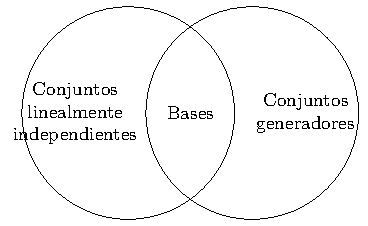
\includegraphics[width=0.55\textwidth]{figuras/venn-bases.pdf}
        \caption{Relación entre conjuntos linealmente independientes, conjuntos generadores y bases.}
    \end{figure}

    \subsection*{La dimensión de los subespacios}

    Nuestro siguiente resultado relaciona la dimensión de un subespacio con la dimensión del espacio vectorial que lo contiene.

    \begin{teorema}
        Sea $W$ un subespacio de un espacio vectorial de dimensión finita $V$. Entonces $W$ es de dimensión finita y $\dim(W)\leq\dim(V)$. Más aún, si $\dim(W)=\dim(V)$, entonces $V=W$.
    \end{teorema}

    \begin{proof}
        Sea $\dim(V)=n$. Si $W=\{0\}$, entonces $W$ es de dimensión finita y $\dim(W)=0\leq n$. En caso contrario, $W$ contiene un vector no nulo $x_1$; así $\{x_1\}$ es un conjunto linealmente independiente. Continuamos eligiendo vectores $x_1,x_2,\dots,x_k$ en $W$ tales que $\{x_1,x_2,\dots,x_k\}$ sea linealmente independiente. Como ningún subconjunto linealmente independiente de $V$ puede contener más de $n$ vectores, este proceso debe detenerse en una etapa en la que $k\leq n$ y $\{x_1,x_2,\dots,x_k\}$ es linealmente independiente, pero agregarle cualquier otro vector de $W$ produce un conjunto linealmente dependiente. El Teorema~1.7 implica que $\{x_1,x_2,\dots,x_k\}$ genera a $W$, y por tanto es una base para $W$. Por tanto $\dim(W)=k\leq n$.

        Si $\dim(W)=n$, entonces una base para $W$ es un subconjunto linealmente independiente de $V$ que contiene $n$ vectores. Pero el corolario 2 al teorema de reemplazo implica que esta base para $W$ es también una base para $V$; así $W=V$.
    \end{proof}

    \begin{ejemplo}
        Sea
        \begin{equation*}
            W=\{(a_1,a_2,a_3,a_4,a_5)\in F^5:a_1+a_3+a_5=0,\ a_2=a_4\}.
        \end{equation*}
        Es fácil mostrar que $W$ es un subespacio de $F^5$ que tiene como base
        \begin{equation*}
            \{(-1,0,1,0,0),(-1,0,0,0,1),(0,1,0,1,0)\}.
        \end{equation*}
        Así $\dim(W)=3$.
    \end{ejemplo}

    \begin{ejemplo}
        El conjunto de las matrices diagonales $n\times n$ es un subespacio $W$ de $M_{n\times n}(F)$ (véase el Ejemplo~12 de la Sección~1.3). Una base para $W$ es
        \begin{equation*}
            \{E^{11},E^{22},\dots,E^{nn}\},
        \end{equation*}
        donde $E^{ij}$ es la matriz cuya única entrada no nula es un $1$ en el renglón $i$ y la columna $j$. Así $\dim(W)=n$.
    \end{ejemplo}

    \begin{ejemplo}
        Vimos en la Sección~1.3 que el conjunto de las matrices simétricas $n\times n$ es un subespacio $W$ de $M_{n\times n}(F)$. Una base para $W$ es
        \begin{equation*}
            \{A^{ij}:1\leq i\leq j\leq n\},
        \end{equation*}
        donde $A^{ij}$ es la matriz $n\times n$ que tiene $1$ en el renglón $i$ y la columna $j$, un $1$ en el renglón $j$ y la columna $i$, y $0$ en las demás entradas. Se sigue que
        \begin{equation*}
            \dim(W)=n+(n-1)+\cdots+1=\tfrac12n(n+1).
        \end{equation*}
    \end{ejemplo}

    \begin{corolario}
        Si $W$ es un subespacio de un espacio vectorial de dimensión finita $V$, entonces cualquier base para $W$ puede extenderse a una base para $V$.
    \end{corolario}

    \begin{proof}
        Sea $S$ una base para $W$. Como $S$ es un subconjunto linealmente independiente de $V$, el corolario~2 al teorema de reemplazo garantiza que $S$ puede extenderse a una base para $V$.
    \end{proof}

    \begin{ejemplo}
        El conjunto de todos los polinomios de la forma
        \begin{equation*}
            a_{18}x^{18}+a_{16}x^{16}+\cdots+a_2x^2+a_0,
        \end{equation*}
        donde $a_{18},a_{16},\dots,a_2,a_0\in F$, es un subespacio $W$ de $P_{18}(F)$. Una base para $W$ es $\{1,x^2,\dots,x^{16},x^{18}\}$, la cual es un subconjunto de la base canónica para $P_{18}(F)$.
    \end{ejemplo}

    Podemos aplicar el Teorema~1.11 para determinar los subespacios de $\R^2$ y de $\R^3$. Como $\R^2$ tiene dimensión $2$, los subespacios de $\R^2$ pueden ser de dimensiones $0$, $1$, o $2$ solamente. Los únicos subespacios de dimensión $0$ o $2$ son $\{0\}$ y $\R^2$, respectivamente. Cualquier subespacio de $\R^2$ que tenga dimensión $1$ consiste de todos los múltiplos escalares de algún vector no nulo en $\R^2$ (Ejercicio~71 de la Sección~1.4).

    Si un punto de $\R^2$ se identifica de la manera natural con un punto del plano euclidiano, entonces es posible describir los subespacios de $\R^2$ geométricamente: un subespacio de $\R^2$ de dimensión $0$ consiste del origen del plano euclidiano, un subespacio de $\R^2$ de dimensión $1$ consiste de una recta que pasa por el origen, y un subespacio de $\R^2$ de dimensión $2$ es el plano euclidiano completo.

    De manera análoga, los subespacios de $\R^3$ deben tener dimensiones $0$, $1$, $2$ o $3$. Interpretando estas posibilidades geométricamente, vemos que un subespacio de dimensión cero debe ser el origen del espacio euclidiano de tres dimensiones, un subespacio de dimensión $1$ es una recta que pasa por el origen, un subespacio de dimensión $2$ es un plano que pasa por el origen, y un subespacio de dimensión $3$ es el espacio euclidiano de tres dimensiones mismo.

    \subsection*{La fórmula de interpolación de Lagrange}

    El corolario~2 del teorema de reemplazo puede aplicarse para obtener una fórmula útil. Sean $c_0,c_1,\dots,c_n$ escalares distintos en un campo infinito $F$. Los polinomios $f_0(x),f_1(x),\dots,f_n(x)$ definidos por
    \begin{equation*}
        f_i(x)=\frac{(x-c_0)\cdots(x-c_{i-1})(x-c_{i+1})\cdots(x-c_n)}{(c_i-c_0)\cdots(c_i-c_{i-1})(c_i-c_{i+1})\cdots(c_i-c_n)}=\prod_{\substack{k=0\\k\neq i}}^{n}\frac{x-c_k}{c_i-c_k}
    \end{equation*}
    se llaman los \textbf{polinomios de Lagrange} (asociados a $c_0,c_1,\dots,c_n$). Notemos que cada $f_i(x)$ es un polinomio de grado $n$ y por tanto está en $P_n(F)$. Considerando a $f_i(x)$ como una función polinomial $f_i:F\to F$, vemos que
    \begin{equation*}
        f_i(c_j)=\begin{cases}0&\text{si }i\neq j\\1&\text{si }i=j.\end{cases}\tag{10}
    \end{equation*}

    Esta propiedad de los polinomios de Lagrange puede usarse para mostrar que $\BB=\{f_0,f_1,\dots,f_n\}$ es un subconjunto linealmente independiente de $P_n(F)$. Supongamos que
    \begin{equation*}
        \sum_{i=0}^{n}a_if_i=0 \qquad\text{para algunos escalares }a_0,a_1,\dots,a_n,
    \end{equation*}
    donde $0$ denota la función cero. Entonces
    \begin{equation*}
        \sum_{i=0}^{n}a_if_i(c_j)=0 \qquad\text{para }j=0,1,\dots,n.
    \end{equation*}
    Pero también
    \begin{equation*}
        \sum_{i=0}^{n}a_if_i(c_j)=a_j
    \end{equation*}
    por (10). De aquí $a_j=0$ para $j=0,1,\dots,n$; así $\BB$ es linealmente independiente. Como la dimensión de $P_n(F)$ es $n+1$, se sigue del inciso (b) del corolario del teorema de reemplazo que $\BB$ es una base para $P_n(F)$.

    Como $\BB$ es una base para $P_n(F)$, toda función polinomial $g$ en $P_n(F)$ es una combinación lineal de los polinomios de $\BB$, digamos
    \begin{equation*}
        g=\sum_{i=0}^{n}b_if_i.
    \end{equation*}
    Se sigue que
    \begin{equation*}
        g(c_j)=\sum_{i=0}^{n}b_if_i(c_j)=b_j;
    \end{equation*}
    así
    \begin{equation*}
        g=\sum_{i=0}^{n}g(c_i)f_i
    \end{equation*}
    es la representación única de $g$ como combinación lineal de elementos de $\BB$. A esta representación se le llama la \textbf{fórmula de interpolación de Lagrange}. Notemos que el argumento anterior muestra que, si $b_0,b_1,\dots,b_n$ son cualesquiera $n+1$ escalares en $F$ (no necesariamente distintos), entonces la función polinomial
    \begin{equation*}
        g=\sum_{i=0}^{n}b_if_i
    \end{equation*}
    es el único polinomio en $P_n(F)$ tal que $g(c_j)=b_j$. Así hemos encontrado el único polinomio de grado a lo más $n$ que tiene valores especificados $b_j$ en los puntos dados $c_j$ ($j=0,1,\dots,n$) de su dominio.

    Por ejemplo, construyamos el polinomio real $g$ de grado a lo más $2$ cuya gráfica contiene los puntos $(1,8)$, $(2,5)$ y $(3,-4)$. (Así, en la notación anterior, $c_0=1$, $c_1=2$, $c_2=3$, $b_0=8$, $b_1=5$, y $b_2=-4$.) Los polinomios de Lagrange asociados a $c_0,c_1$ y $c_2$ son
    \begin{equation*}
        f_0(x)=\frac{(x-2)(x-3)}{(1-2)(1-3)}=\tfrac12(x^2-5x+6),
    \end{equation*}
    \begin{equation*}
        f_1(x)=\frac{(x-1)(x-3)}{(2-1)(2-3)}=-1(x^2-4x+3),
    \end{equation*}
    y
    \begin{equation*}
        f_2(x)=\frac{(x-1)(x-2)}{(3-1)(3-2)}=\tfrac12(x^2-3x+2).
    \end{equation*}
    Por tanto el polinomio deseado es
    \begin{align*}
        g(x)=\sum_{i=0}^{2}b_if_i(x)&=8f_0(x)+5f_1(x)-4f_2(x)\\
        &=4(x^2-5x+6)-5(x^2-4x+3)-2(x^2-3x+2)\\
        &=-3x^2+6x+5.
    \end{align*}

    Una consecuencia importante de la fórmula de interpolación de Lagrange es el siguiente resultado: si $f\in P_n(F)$ y $f(c_i)=0$ para $n+1$ escalares distintos $c_0,c_1,\dots,c_n$ en $F$, entonces $f$ es la función cero.

    \begin{ejercicio}
        Etiquete las siguientes afirmaciones como verdaderas o falsas.
        \begin{enumerate}[label=(\alph*)]
            \item El espacio vectorial cero no tiene base.
            \item Todo espacio vectorial que es generado por un conjunto finito tiene una base.
            \item Todo espacio vectorial tiene una base finita.
            \item Un espacio vectorial no puede tener más de una base.
            \item Si un espacio vectorial tiene una base finita, entonces el número de vectores en cada base es el mismo.
            \item La dimensión de $P_n(F)$ es $n$.
            \item La dimensión de $M_{m\times n}(F)$ es $m+n$.
            \item Supongamos que $V$ es un espacio vectorial de dimensión finita, que $S_1$ es un subconjunto de $V$ que es linealmente independiente, y que $S_2$ es un subconjunto de $V$ que genera a $V$. Entonces $S_1$ no puede contener más vectores que $S_2$.
            \item Si $S$ genera al espacio vectorial $V$, entonces cada vector de $V$ puede escribirse como combinación lineal de vectores de $S$ de una sola manera.
            \item Todo subespacio de un espacio de dimensión finita es de dimensión finita.
            \item Si $V$ es un espacio vectorial con dimensión $n$, entonces $V$ tiene exactamente un subespacio de dimensión $0$ y exactamente un subespacio de dimensión $n$.
            \item Si $V$ es un espacio vectorial con dimensión $n$, y si $S$ es un subconjunto de $V$ con $n$ vectores, entonces $S$ es linealmente independiente si y solo si $S$ genera a $V$.
        \end{enumerate}
    \end{ejercicio}

    \begin{ejercicio}
        Determine cuáles de los siguientes conjuntos son bases para $\R^3$.
        \begin{enumerate}[label=(\alph*)]
            \item $\{(1,0,-1),(2,5,1),(0,-4,3)\}$
            \item $\{(2,-4,1),(0,3,-1),(6,0,-1)\}$
            \item $\{(1,2,-1),(1,0,2),(2,1,1)\}$
            \item $\{(-1,3,1),(2,-4,-3),(-3,8,2)\}$
            \item $\{(1,-3,-2),(-3,1,3),(-2,-10,-2)\}$
        \end{enumerate}
    \end{ejercicio}

    \begin{ejercicio}
        Determine cuáles de los siguientes conjuntos son bases para $P_2(\R)$.
        \begin{enumerate}[label=(\alph*)]
            \item $\{-1-x+2x^2,\,2+x-2x^2,\,1-2x+4x^2\}$
            \item $\{1+2x+x^2,\,3+x^2,\,x+x^2\}$
            \item $\{1-2x-2x^2,\,-2+3x-x^2,\,1-x+6x^2\}$
            \item $\{-1+2x+4x^2,\,3-4x-10x^2,\,-2-5x-6x^2\}$
            \item $\{1+2x-x^2,\,4-2x+x^2,\,-1+18x-9x^2\}$
        \end{enumerate}
    \end{ejercicio}

    \begin{ejercicio}
        ¿Generan los polinomios $x^3-2x^2+1$, $4x^2-x+3$ y $3x-2$ a $P_3(\R)$? Justifique su respuesta.
    \end{ejercicio}

    \begin{ejercicio}
        ¿Es $\{(1,4,-6),(1,5,8),(2,1,1),(0,1,0)\}$ un subconjunto linealmente independiente de $\R^3$? Justifique su respuesta.
    \end{ejercicio}

    \begin{ejercicio}
        Dé tres bases distintas para $F^2$ y para $M_{2\times 2}(F)$.
    \end{ejercicio}

    \begin{ejercicio}
        Los vectores $u_1=(2,-3,1)$, $u_2=(1,4,-2)$, $u_3=(-8,12,-4)$, $u_4=(1,37,-17)$, y $u_5=(-3,-5,8)$ generan a $\R^3$. Encuentre un subconjunto del conjunto $\{u_1,u_2,u_3,u_4,u_5\}$ que sea una base para $\R^3$.
    \end{ejercicio}

    \begin{ejercicio}
        Sea $W$ el subespacio de $\R^5$ que consiste de todos los vectores cuyas coordenadas suman cero. Los vectores
        \begin{align*}
            u_1&=(2,-3,4,-5,2), & u_2&=(-6,9,-12,15,-6),\\
            u_3&=(3,-2,7,-9,1), & u_4&=(2,-8,2,-2,6),\\
            u_5&=(-1,1,2,1,-3), & u_6&=(0,-3,-18,9,12),\\
            u_7&=(1,0,-2,3,-2), & u_8&=(2,-1,1,-9,7)
        \end{align*}
        generan a $W$. Encuentre un subconjunto del conjunto $\{u_1,u_2,\dots,u_8\}$ que sea una base para $W$.
    \end{ejercicio}

    \begin{ejercicio}
        Los vectores $u_1=(1,1,1,1)$, $u_2=(0,1,1,1)$, $u_3=(0,0,1,1)$, y $u_4=(0,0,0,1)$ forman una base para $F^4$. Encuentre la representación única de un vector arbitrario $(a_1,a_2,a_3,a_4)$ en $F^4$ como combinación lineal de $u_1,u_2,u_3$ y $u_4$.
    \end{ejercicio}

    \begin{ejercicio}
        En cada inciso, use la fórmula de interpolación de Lagrange para construir el polinomio de menor grado cuya gráfica contenga los siguientes puntos.
        \begin{enumerate}[label=(\alph*)]
            \item $(-2,-6)$, $(-1,5)$, $(1,3)$
            \item $(-4,24)$, $(1,9)$, $(3,3)$
            \item $(-2,3)$, $(-1,-6)$, $(1,0)$, $(3,-2)$
            \item $(-3,-30)$, $(-2,7)$, $(0,15)$, $(1,10)$
        \end{enumerate}
    \end{ejercicio}

    \begin{ejercicio}
        Sean $u$ y $v$ vectores distintos de un espacio vectorial $V$. Muestre que si $\{u,v\}$ es una base para $V$ y $a$ y $b$ son escalares no nulos, entonces tanto $\{u+v,au\}$ como $\{au,bv\}$ son también bases para $V$.
    \end{ejercicio}

    \begin{ejercicio}
        Sean $u$, $v$ y $w$ vectores distintos de un espacio vectorial $V$. Muestre que si $\{u,v,w\}$ es una base para $V$, entonces $\{u+v+w,v+w,w\}$ también es una base para $V$.
    \end{ejercicio}

    \begin{ejercicio}
        El conjunto de soluciones del sistema de ecuaciones lineales
        \begin{align*}
            x_1-2x_2+x_3&=0\\
            2x_1-3x_2+x_3&=0
        \end{align*}
        es un subespacio de $\R^3$. Encuentre una base para este subespacio.
    \end{ejercicio}

    \begin{ejercicio}
        Encuentre bases para los siguientes subespacios de $F^5$:
        \begin{equation*}
            W_1=\{(a_1,a_2,a_3,a_4,a_5)\in F^5:a_1-a_3-a_4=0\}
        \end{equation*}
        y
        \begin{equation*}
            W_2=\{(a_1,a_2,a_3,a_4,a_5)\in F^5:a_2=a_3=a_4\text{ y }a_1+a_5=0\}.
        \end{equation*}
        ¿Cuáles son las dimensiones de $W_1$ y $W_2$?
    \end{ejercicio}

    \begin{ejercicio}
        El conjunto de todas las matrices $n\times n$ con traza igual a cero es un subespacio $W$ de $M_{n\times n}(F)$ (véase el Ejemplo~13 de la Sección~1.3). Encuentre una base para $W$. ¿Cuál es la dimensión de $W$?
    \end{ejercicio}

    \begin{ejercicio}
        El conjunto de todas las matrices triangulares superiores $n\times n$ es un subespacio $W$ de $M_{n\times n}(F)$ (véase el Ejercicio~41 de la Sección~1.3). Encuentre una base para $W$. ¿Cuál es la dimensión de $W$?
    \end{ejercicio}

    \begin{ejercicio}
        El conjunto de todas las matrices antisimétricas $n\times n$ es un subespacio $W$ de $M_{n\times n}(F)$ (véase el Ejercicio~57 de la Sección~1.3). Encuentre una base para $W$. ¿Cuál es la dimensión de $W$?
    \end{ejercicio}

    \begin{ejercicio}
        Encuentre una base para el espacio vectorial del Ejemplo~7 de la Sección~1.2. Justifique su respuesta.
    \end{ejercicio}

    \begin{ejercicio}
        Complete la demostración del Teorema~1.8.
    \end{ejercicio}

    \begin{ejercicio}
        Sea $V$ un espacio vectorial de dimensión $n$, y sea $S$ un subconjunto de $V$ que genera a $V$.
        \begin{enumerate}[label=(\alph*)]
            \item Pruebe que existe un subconjunto de $S$ que es una base para $V$. (Tenga cuidado de no suponer que $S$ es finito.)
            \item Pruebe que $S$ contiene al menos $n$ vectores.
        \end{enumerate}
    \end{ejercicio}

    \begin{ejercicio}
        Pruebe que un espacio vectorial es de dimensión infinita si y solo si contiene un subconjunto linealmente independiente infinito.
    \end{ejercicio}

    \begin{ejercicio}
        Sean $W_1$ y $W_2$ subespacios de un espacio vectorial de dimensión finita $V$. Determine condiciones necesarias y suficientes sobre $W_1$ y $W_2$ para que $\dim(W_1\cap W_2)=\dim(W_1)$.
    \end{ejercicio}

    \begin{ejercicio}
        Sean $v_1,v_2,\dots,v_k,v$ vectores de un espacio vectorial $V$, y definamos $W_1=\gen{\{v_1,v_2,\dots,v_k\}}$ y $W_2=\gen{\{v_1,v_2,\dots,v_k,v\}}$.
        \begin{enumerate}[label=(\alph*)]
            \item Encuentre condiciones necesarias y suficientes sobre $v$ tales que $\dim(W_1)=\dim(W_2)$.
            \item Enuncie y pruebe una relación que involucre a $\dim(W_1)$ y $\dim(W_2)$, en el caso de que $\dim(W_1)\neq\dim(W_2)$.
        \end{enumerate}
    \end{ejercicio}

    \begin{ejercicio}
        Sea $f(x)$ un polinomio de grado $n$ en $P_n(\R)$. Pruebe que, para cualquier $g(x)\in P_n(\R)$, existen escalares $c_0,c_1,\dots,c_n$ tales que
        \begin{equation*}
            g(x)=c_0f(x)+c_1f'(x)+c_2f''(x)+\cdots+c_nf^{(n)}(x),
        \end{equation*}
        donde $f^{(n)}(x)$ denota la $n$-ésima derivada de $f(x)$.
    \end{ejercicio}

    \begin{ejercicio}
        Sean $V$, $W$ y $Z$ como en el Ejercicio~28 de la Sección~1.2. Si $V$ y $W$ son espacios vectoriales sobre $F$ de dimensiones $m$ y $n$, determine la dimensión de $Z$.
    \end{ejercicio}

    \begin{ejercicio}
        Para un $a\in\R$ fijo, determine la dimensión del subespacio de $P_n(\R)$ definido por $\{f\in P_n(\R):f(a)=0\}$.
    \end{ejercicio}

    \begin{ejercicio}
        Sean $W_1$ y $W_2$ los subespacios de $P(F)$ definidos en el Ejercicio~54 de la Sección~1.3. Determine las dimensiones de los subespacios $W_1\cap P_n(F)$ y $W_2\cap P_n(F)$.
    \end{ejercicio}

    \begin{ejercicio}
        Sea $V$ un espacio vectorial de dimensión finita sobre $\C$ con dimensión $n$. Pruebe que, si $V$ se considera ahora como un espacio vectorial sobre $\R$, entonces $\dim V=2n$. (Véanse los Ejemplos~11 y 12.)
    \end{ejercicio}

    Los Ejercicios~29 a 34 requieren conocer la suma y la suma directa de subespacios, tal como se definieron en los ejercicios de la Sección~1.3.

    \begin{ejercicio}
        \begin{enumerate}[label=(\alph*)]
            \item Pruebe que si $W_1$ y $W_2$ son subespacios de dimensión finita de un espacio vectorial $V$, entonces el subespacio $W_1+W_2$ es de dimensión finita, y
            \begin{equation*}
                \dim(W_1+W_2)=\dim(W_1)+\dim(W_2)-\dim(W_1\cap W_2).
            \end{equation*}
            (\textit{Sugerencia:} Comience con una base $\{u_1,u_2,\dots,u_k\}$ para $W_1\cap W_2$, y extiéndala a una base $\{u_1,u_2,\dots,u_k,v_1,v_2,\dots,v_m\}$ para $W_1$ y a una base $\{u_1,u_2,\dots,u_k,w_1,w_2,\dots,w_p\}$ para $W_2$.)
            \item Sean $W_1$ y $W_2$ subespacios de dimensión finita de un espacio vectorial $V$, y supongamos que $V=W_1+W_2$. Deduzca que $V$ es la suma directa de $W_1$ y $W_2$ si y solo si $\dim(V)=\dim(W_1)+\dim(W_2)$.
        \end{enumerate}
    \end{ejercicio}

    \begin{ejercicio}
        Sean
        \begin{equation*}
            V=M_{2\times 2}(F), \qquad W_1=\left\{\begin{pmatrix}a&b\\c&a\end{pmatrix}\in V:a,b,c\in F\right\},
        \end{equation*}
        y
        \begin{equation*}
            W_2=\left\{\begin{pmatrix}0&a\\-a&b\end{pmatrix}\in V:a,b\in F\right\}.
        \end{equation*}
        Pruebe que $W_1$ y $W_2$ son subespacios de $V$, y encuentre las dimensiones de $W_1$, $W_2$, $W_1+W_2$, y $W_1\cap W_2$.
    \end{ejercicio}

    \begin{ejercicio}
        Sean $W_1$ y $W_2$ subespacios de un espacio vectorial $V$ que tienen dimensiones $m$ y $n$, respectivamente, donde $m\geq n$.
        \begin{enumerate}[label=(\alph*)]
            \item Pruebe que $\dim(W_1\cap W_2)\leq n$.
            \item Pruebe que $\dim(W_1+W_2)\leq m+n$.
        \end{enumerate}
    \end{ejercicio}

    \begin{ejercicio}
        \begin{enumerate}[label=(\alph*)]
            \item Encuentre un ejemplo de subespacios $W_1$ y $W_2$ de $\R^3$, con dimensiones $m$ y $n$, donde $m>n>0$, tales que $\dim(W_1\cap W_2)=n$.
            \item Encuentre un ejemplo de subespacios $W_1$ y $W_2$ de $\R^3$, con dimensiones $m$ y $n$, donde $m>n>0$, tales que $\dim(W_1+W_2)=m+n$.
            \item Encuentre un ejemplo de subespacios $W_1$ y $W_2$ de $\R^3$, con dimensiones $m$ y $n$, donde $m\geq n$, tales que $\dim(W_1\cap W_2)<n$ y $\dim(W_1+W_2)<m+n$.
        \end{enumerate}
    \end{ejercicio}

    \begin{ejercicio}
        \begin{enumerate}[label=(\alph*)]
            \item Sean $W_1$ y $W_2$ subespacios de un espacio vectorial $V$ tales que $V=W_1\oplus W_2$. Si $\beta_1$ y $\beta_2$ son bases para $W_1$ y $W_2$, respectivamente, muestre que $\beta_1\cap\beta_2=\emptyset$ y $\beta_1\cup\beta_2$ es una base para $V$.
            \item Recíprocamente, sean $\beta_1$ y $\beta_2$ bases disjuntas para subespacios $W_1$ y $W_2$, respectivamente, de un espacio vectorial $V$. Pruebe que, si $\beta_1\cup\beta_2$ es una base para $V$, entonces $V=W_1\oplus W_2$.
        \end{enumerate}
    \end{ejercicio}

    \begin{ejercicio}
        \begin{enumerate}[label=(\alph*)]
            \item Pruebe que, si $W_1$ es cualquier subespacio de un espacio vectorial de dimensión finita $V$, entonces existe un subespacio $W_2$ de $V$ tal que $V=W_1\oplus W_2$.
            \item Sea $V=\R^2$ y $W_1=\{(a_1,0):a_1\in\R\}$. Dé ejemplos de dos subespacios distintos $W_2$ y $W_2'$ tales que $V=W_1\oplus W_2$ y $V=W_1\oplus W_2'$.
        \end{enumerate}
    \end{ejercicio}

    El siguiente ejercicio requiere familiaridad con el Ejercicio~60 de la Sección~1.3.

    \begin{ejercicio}
        Sea $W$ un subespacio de un espacio vectorial de dimensión finita $V$, y consideremos una base $\{u_1,u_2,\dots,u_k\}$ para $W$. Sea $\{u_1,u_2,\dots,u_k,u_{k+1},\dots,u_n\}$ una extensión de esta base a una base para $V$.
        \begin{enumerate}[label=(\alph*)]
            \item Pruebe que $\{u_{k+1}+W,u_{k+2}+W,\dots,u_n+W\}$ es una base para $V/W$.
            \item Deduzca una fórmula que relacione $\dim(V)$, $\dim(W)$, y $\dim(V/W)$.
        \end{enumerate}
    \end{ejercicio}

    \section{Subconjuntos linealmente independientes maximales}

    En esta sección, opcional, varios resultados significativos de la Sección~1.6 se extienden a espacios vectoriales de dimensión infinita. Nuestro objetivo principal aquí es probar que todo espacio vectorial tiene una base. Este resultado es importante en el estudio de los espacios vectoriales de dimensión infinita porque a menudo es difícil construir explícitamente una base para tal espacio. Consideremos, por ejemplo, el espacio vectorial de los números reales sobre el campo de los números racionales. No hay una manera obvia de construir una base para este espacio, y sin embargo se sigue de los resultados de esta sección que tal base existe.

    La dificultad que surge al extender los teoremas de la sección anterior a espacios vectoriales de dimensión infinita es que el principio de inducción matemática, que desempeñó un papel crucial en muchas de las demostraciones de la Sección~1.6, ya no es adecuado. En su lugar, se necesita un resultado más general llamado el \textit{principio maximal}. Antes de enunciar este principio, necesitamos introducir algo de terminología.

    \begin{definicion}[Cadena]
        Una colección $\mathcal{C}$ de conjuntos se llama \textbf{cadena} (o \textbf{nido} o \textbf{torre}) si, para cada par de conjuntos $A$ y $B$ en $\mathcal{C}$, se tiene $A\subseteq B$ o $B\subseteq A$.
    \end{definicion}

    \begin{ejemplo}
        Sea $\mathcal{F}$ la familia de todos los subconjuntos de un conjunto no vacío $S$. (A esta familia $\mathcal{F}$ se le llama el \textbf{conjunto potencia} de $S$.) Es fácil ver que $S$ es un elemento maximal de $\mathcal{F}$.
    \end{ejemplo}

    \begin{ejemplo}
        Sean $S$ y $T$ conjuntos no vacíos disjuntos, y sea $\mathcal{F}$ la unión de sus conjuntos potencia. Entonces $S$ y $T$ son ambos elementos maximales de $\mathcal{F}$.
    \end{ejemplo}

    \begin{ejemplo}
        Sea $\mathcal{F}$ la familia de todos los subconjuntos finitos de un conjunto infinito $S$. Entonces $\mathcal{F}$ no tiene elemento maximal. Pues, si $M$ es cualquier elemento de $\mathcal{F}$ y $s$ es cualquier elemento de $S$ que no está en $M$, entonces $M\cup\{s\}$ es un elemento de $\mathcal{F}$ que contiene a $M$ como subconjunto propio.
    \end{ejemplo}

    \begin{ejemplo}
        Para cada entero positivo $n$, sea $A_n=\{1,2,\dots,n\}$. Entonces la colección de conjuntos $\mathcal{C}=\{A_n:n=1,2,3,\dots\}$ es una cadena. De hecho, $A_m\subseteq A_n$ si y solo si $m\leq n$.
    \end{ejemplo}

    Con esta terminología, podemos ahora enunciar el principio maximal.

    \begin{teorema}[Principio maximal]
        Sea $\mathcal{F}$ una familia de conjuntos. Si, para cada cadena $\mathcal{C}\subseteq\mathcal{F}$, existe un miembro de $\mathcal{F}$ que contiene a cada miembro de $\mathcal{C}$, entonces $\mathcal{F}$ contiene un elemento maximal.\footnote{El principio maximal es lógicamente equivalente al axioma de elección, el cual es una suposición común en los desarrollos axiomáticos de la teoría de conjuntos. Para un tratamiento de la teoría de conjuntos usando el principio maximal, véase John L. Kelley, \textit{General Topology}, Graduate Texts in Mathematics Series, Vol.~27, Springer-Verlag, 1991.}
    \end{teorema}

    Como el principio maximal garantiza la existencia de elementos maximales en una familia de conjuntos que satisface la hipótesis anterior, resulta útil reformular la definición de base en términos de una propiedad maximal. En el Teorema~1.13 mostramos que esto es posible; de hecho, el concepto que se define a continuación es equivalente al de base.

    \begin{definicion}[Subconjunto linealmente independiente maximal]
        Sea $S$ un subconjunto de un espacio vectorial $V$. Un \textbf{subconjunto linealmente independiente maximal} de $S$ es un subconjunto $\BB$ de $S$ que satisface ambas condiciones siguientes:
        \begin{enumerate}[label=(\alph*)]
            \item $\BB$ es linealmente independiente.
            \item El único subconjunto linealmente independiente de $S$ que contiene a $\BB$ es $\BB$ mismo.
        \end{enumerate}
    \end{definicion}

    \begin{ejemplo}
        El Ejemplo~16 de la Sección~1.4 muestra que
        \begin{equation*}
            \{x^3-2x^2-5x-3,\,3x^3-5x^2-4x-9\}
        \end{equation*}
        es un subconjunto linealmente independiente maximal de
        \begin{equation*}
            S=\{2x^3-2x^2+12x-6,\,x^3-2x^2-5x-3,\,3x^3-5x^2-4x-9\}
        \end{equation*}
        en $P_2(\R)$. En este caso, sin embargo, se muestra fácilmente que cualquier subconjunto de $S$ que consista de dos polinomios es un subconjunto linealmente independiente maximal de $S$. Así los subconjuntos linealmente independientes maximales de un conjunto no necesitan ser únicos.
    \end{ejemplo}

    Una base $\BB$ para un espacio vectorial $V$ es un subconjunto linealmente independiente maximal de $V$, pues:
    \begin{enumerate}
        \item $\BB$ es linealmente independiente por definición.
        \item Si $v\in V$ y $v\notin\BB$, entonces $\BB\cup\{v\}$ es linealmente dependiente por el Teorema~1.7, ya que $\gen{\BB}=V$.
    \end{enumerate}

    Nuestro siguiente resultado muestra que el recíproco de esta afirmación también es cierto.

    \begin{teorema}
        Sea $V$ un espacio vectorial y $S$ un subconjunto que genera a $V$. Si $\BB$ es un subconjunto linealmente independiente maximal de $S$, entonces $\BB$ es una base para $V$.
    \end{teorema}

    \begin{proof}
        Sea $\BB$ un subconjunto linealmente independiente maximal de $S$. Como $\BB$ es linealmente independiente, basta probar que $\BB$ genera a $V$. Afirmamos que $S\subseteq\gen{\BB}$, pues de lo contrario existe $v\in S$ tal que $v\notin\gen{\BB}$. Como el Teorema~1.7 implica que $\BB\cup\{v\}$ es linealmente independiente, hemos contradicho la maximalidad de $\BB$. Por tanto $S\subseteq\gen{\BB}$. Como $\gen{S}=V$, se sigue del Teorema~1.5 que $\gen{\BB}=V$.
    \end{proof}

    Así un subconjunto de un espacio vectorial es una base si y solo si es un subconjunto linealmente independiente maximal del espacio vectorial. Por tanto podemos lograr nuestro objetivo de probar que todo espacio vectorial tiene una base mostrando que todo espacio vectorial contiene un subconjunto linealmente independiente maximal. Este resultado se sigue inmediatamente del siguiente teorema.

    \begin{teorema}
        Sea $S$ un subconjunto linealmente independiente de un espacio vectorial $V$. Existe un subconjunto linealmente independiente maximal de $V$ que contiene a $S$.
    \end{teorema}

    \begin{proof}
        Sea $\mathcal{F}$ la familia de todos los subconjuntos linealmente independientes de $V$ que contienen a $S$. Para mostrar que $\mathcal{F}$ contiene un elemento maximal, debemos mostrar que si $\mathcal{C}$ es una cadena en $\mathcal{F}$, entonces existe un miembro $U$ de $\mathcal{F}$ que contiene a cada miembro de $\mathcal{C}$. Afirmamos que $U$, la unión de los miembros de $\mathcal{C}$, es el conjunto buscado. Claramente $U$ contiene a cada miembro de $\mathcal{C}$; y, como cada miembro de $\mathcal{C}$ es un subconjunto de $V$ que contiene a $S$, tenemos $S\subseteq U\subseteq V$. Así solo necesitamos probar que $U$ es linealmente independiente.

        Sean $u_1,u_2,\dots,u_n$ elementos de $U$, y sean $a_1,a_2,\dots,a_n$ escalares tales que $a_1u_1+a_2u_2+\cdots+a_nu_n=0$. Como $u_i\in U$ para $i=1,2,\dots,n$, existe un conjunto $A_i$ en $\mathcal{C}$ tal que $u_i\in A_i$. Pero, como $\mathcal{C}$ es una cadena, uno de estos conjuntos, digamos $A_k$, contiene a todos los demás. Así $u_i\in A_k$ para $i=1,2,\dots,n$. Sin embargo, $A_k$ es un conjunto linealmente independiente; así $a_1u_1+a_2u_2+\cdots+a_nu_n=0$ implica que $a_1=a_2=\cdots=a_n=0$. Se sigue que $U$ es linealmente independiente.

        El principio maximal implica que $\mathcal{F}$ tiene un elemento maximal. Este elemento se ve fácilmente que es un subconjunto linealmente independiente maximal de $V$ que contiene a $S$.
    \end{proof}

    \begin{corolario}
        Todo espacio vectorial tiene una base.
    \end{corolario}

    \begin{proof}
        Sea $V$ un espacio vectorial. Como $\emptyset$ es un subconjunto linealmente independiente de $V$, el teorema anterior implica que existe un subconjunto linealmente independiente maximal $\BB$ de $V$ que contiene a $\emptyset$. Por el Teorema~1.13 (aplicado con $S=V$), $\BB$ es una base para $V$.
    \end{proof}

    Puede mostrarse, de manera análoga al corolario del teorema de reemplazo (Sección~1.6), que toda base para un espacio vectorial de dimensión infinita tiene la misma \textit{cardinalidad}. (Dos conjuntos tienen la misma cardinalidad si existe una correspondencia biunívoca entre ellos.) Véase, por ejemplo, N.~Jacobson, \textit{Lectures in Abstract Algebra}, vol.~2, \textit{Linear Algebra}, D.~Van Nostrand Company, Nueva York, 1953, p.~240.

    Los Ejercicios~4 a 7 extienden otros resultados de la Sección~1.6 a espacios vectoriales de dimensión infinita.

    \begin{ejercicio}
        Etiquete las siguientes afirmaciones como verdaderas o falsas.
        \begin{enumerate}[label=(\alph*)]
            \item Toda familia de conjuntos contiene un elemento maximal.
            \item Toda cadena contiene un elemento maximal.
            \item Si una familia de conjuntos tiene un elemento maximal, entonces ese elemento maximal es único.
            \item Si una cadena de conjuntos tiene un elemento maximal, entonces ese elemento maximal es único.
            \item Una base para un espacio vectorial es un subconjunto linealmente independiente maximal de ese espacio vectorial.
            \item Un subconjunto linealmente independiente maximal de un espacio vectorial es una base para ese espacio vectorial.
        \end{enumerate}
    \end{ejercicio}

    \begin{ejercicio}
        Muestre que el conjunto de las sucesiones convergentes es un subespacio de dimensión infinita del espacio vectorial de todas las sucesiones de números reales. (Véase el Ejercicio~50 de la Sección~1.3.)
    \end{ejercicio}

    \begin{ejercicio}
        Sea $V$ el conjunto de los números reales, considerado como un espacio vectorial sobre el campo de los números racionales. Pruebe que $V$ es de dimensión infinita. \textit{Sugerencia:} Use el hecho de que $\pi$ es trascendente, es decir, que $\pi$ no es raíz de ningún polinomio con coeficientes racionales.
    \end{ejercicio}

    \begin{ejercicio}
        Sea $W$ un subespacio de un espacio vectorial $V$, no necesariamente de dimensión finita. Pruebe que cualquier base para $W$ es un subconjunto de alguna base para $V$.
    \end{ejercicio}

    \begin{ejercicio}
        Pruebe la siguiente versión de dimensión infinita del Teorema~1.8: Sea $\BB$ un subconjunto de un espacio vectorial de dimensión infinita $V$. Entonces $\BB$ es una base para $V$ si y solo si, para cada vector no nulo $v$ de $V$, existen vectores únicos $u_1,u_2,\dots,u_n$ en $\BB$ y escalares no nulos únicos $c_1,c_2,\dots,c_n$ tales que $v=c_1u_1+c_2u_2+\cdots+c_nu_n$.
    \end{ejercicio}

    \begin{ejercicio}
        Pruebe la siguiente generalización del Teorema~1.9: Sean $S_1$ y $S_2$ subconjuntos de un espacio vectorial $V$ tales que $S_1\subseteq S_2$. Si $S_1$ es linealmente independiente y $S_2$ genera a $V$, entonces existe una base $\BB$ para $V$ tal que $S_1\subseteq\BB\subseteq S_2$. \textit{Sugerencia:} Aplique el principio maximal a la familia de todos los subconjuntos linealmente independientes de $S_2$ que contienen a $S_1$, y proceda como en la demostración del Teorema~1.14.
    \end{ejercicio}

    \begin{ejercicio}
        Pruebe la siguiente generalización del teorema de reemplazo. Sea $\BB$ una base para un espacio vectorial $V$, y sea $S$ un subconjunto linealmente independiente de $V$. Existe un subconjunto $S_1$ de $\BB$ tal que $S\cup S_1$ es una base para $V$.
    \end{ejercicio}

    \chapter{Transformaciones lineales y matrices}

    En el Capítulo~1 desarrollamos con cierto detalle la teoría de los espacios vectoriales abstractos. Es natural ahora considerar aquellas funciones definidas sobre espacios vectoriales que, en cierto sentido, \textquotedblleft preservan\textquotedblright\ la estructura. A estas funciones especiales se les llama \textbf{transformaciones lineales}, y abundan tanto en la matemática pura como en la aplicada. En cálculo, las operaciones de derivación e integración nos proporcionan dos de los ejemplos más importantes de transformaciones lineales (véanse los Ejemplos~6 y 7 de la Sección~2.1). Estos dos ejemplos nos permiten reformular muchos de los problemas de ecuaciones diferenciales e integrales en términos de transformaciones lineales sobre espacios vectoriales particulares (véase la Sección~2.7).

    En geometría, las rotaciones, reflexiones y proyecciones (véanse los Ejemplos~2, 3 y 4 de la Sección~2.1) nos proporcionan otra clase de transformaciones lineales. Más adelante, usamos estas transformaciones para estudiar los movimientos rígidos en $\R^n$.

    En los capítulos siguientes veremos más ejemplos de transformaciones lineales que aparecen tanto en las ciencias físicas como en las sociales. A lo largo de este capítulo, suponemos que todos los espacios vectoriales están sobre un campo común $F$.

    \section{Transformaciones lineales, espacios nulos y rangos}

    En esta sección consideramos varios ejemplos de transformaciones lineales. Muchas de estas transformaciones se estudian con más detalle en secciones posteriores. Recordemos que una función $T$ con dominio $V$ y codominio $W$ se denota $T:V\to W$.

    \begin{definicion}[Transformación lineal]
        Sean $V$ y $W$ espacios vectoriales (sobre $F$). Llamamos a una función $T:V\to W$ una \textbf{transformación lineal} de $V$ a $W$ si, para todos $x,y\in V$ y $c\in F$, tenemos
        \begin{enumerate}[label=(\alph*)]
            \item $T(x+y)=T(x)+T(y)$, y
            \item $T(cx)=cT(x)$.
        \end{enumerate}
    \end{definicion}

    Si el campo subyacente $F$ es el campo de los números racionales, entonces (a) implica (b) (véase el Ejercicio~38), pero, en general, (a) y (b) son lógicamente independientes (véanse los Ejercicios~39 y 40).

    Con frecuencia llamamos a $T$ simplemente \textbf{lineal}. El lector debe verificar las siguientes propiedades de una función $T:V\to W$ (véase el Ejercicio~8).
    \begin{enumerate}
        \item Si $T$ es lineal, entonces $T(0)=0$.
        \item $T$ es lineal si y solo si $T(cx+y)=cT(x)+T(y)$ para todos $x,y\in V$ y $c\in F$.
        \item Si $T$ es lineal, entonces $T(x-y)=T(x)-T(y)$ para todos $x,y\in V$.
        \item $T$ es lineal si y solo si, para $x_1,x_2,\dots,x_n\in V$ y $a_1,a_2,\dots,a_n\in F$, tenemos
        \begin{equation*}
            T\left(\sum_{i=1}^{n}a_ix_i\right)=\sum_{i=1}^{n}a_iT(x_i).
        \end{equation*}
    \end{enumerate}

    Verificamos brevemente estas propiedades. Para la propiedad 1, si $T$ es lineal, entonces $T(0)=T(0+0)=T(0)+T(0)$, y la ley de cancelación implica que $T(0)=0$. Para la propiedad 2, si $T$ es lineal, entonces claramente $T(cx+y)=T(cx)+T(y)=cT(x)+T(y)$ usando (a) y (b) de la definición. Recíprocamente, si $T(cx+y)=cT(x)+T(y)$ para todos $x,y,c$, tomando $c=1$ obtenemos (a), y tomando $y=0$ (y usando que $T(0)=0$, lo cual se sigue del caso $c=-1$, $y=x$ de la hipótesis: $0=T(-x+x)=-T(x)+T(x)$, cierto trivialmente, pero también $T(0)=T((-1)x+x)=-T(x)+T(x)$ solo confirma consistencia; más directamente, tomando $x=0$ y $c=0$ en la hipótesis, $T(0)=T(0\cdot 0+0)=0\cdot T(0)+T(0)=T(0)$, lo cual no aporta información nueva —para obtener $T(0)=0$ basta notar que $T$ satisface (a) por lo anterior, y entonces la propiedad 1 ya establecida da $T(0)=0$) obtenemos $T(cx)=cT(x)+T(0)=cT(x)$, que es (b). Para la propiedad 3, $T(x-y)=T(x+(-1)y)=T(x)+T((-1)y)=T(x)+(-1)T(y)=T(x)-T(y)$, usando (a) y (b). La propiedad 4 se sigue de (a) y (b) por inducción sobre $n$.

    \begin{ejemplo}
        Definamos
        \begin{equation*}
            T:\R^2\to\R^2 \qquad\text{por}\qquad T(a_1,a_2)=(2a_1+a_2,\,a_1).
        \end{equation*}
        Para mostrar que $T$ es lineal, sean $c\in\R$ y $x,y\in\R^2$, donde $x=(b_1,b_2)$ y $y=(d_1,d_2)$. Como
        \begin{equation*}
            cx+y=(cb_1+d_1,\,cb_2+d_2),
        \end{equation*}
        tenemos
        \begin{equation*}
            T(cx+y)=\big(2(cb_1+d_1)+cb_2+d_2,\;cb_1+d_1\big).
        \end{equation*}
        Además,
        \begin{align*}
            cT(x)+T(y)&=c(2b_1+b_2,\,b_1)+(2d_1+d_2,\,d_1)\\
            &=(2cb_1+cb_2+2d_1+d_2,\;cb_1+d_1)\\
            &=\big(2(cb_1+d_1)+cb_2+d_2,\;cb_1+d_1\big).
        \end{align*}
        Así $T$ es lineal.
    \end{ejemplo}

    Como veremos más adelante, las aplicaciones del álgebra lineal a la geometría son amplias y variadas. La razón principal de esto es que la mayoría de las transformaciones geométricas importantes son lineales. Consideramos ahora tres transformaciones particulares: la rotación, la reflexión y la proyección. Dejamos al lector las demostraciones de linealidad, salvo por un breve comentario en cada caso.

    \begin{ejemplo}
        Para cualquier ángulo $\theta$, definamos $T_\theta:\R^2\to\R^2$ mediante la regla: $T_\theta(a_1,a_2)$ es el vector que se obtiene al rotar $(a_1,a_2)$ en sentido antihorario un ángulo $\theta$ si $(a_1,a_2)\neq(0,0)$, y $T_\theta(0,0)=(0,0)$. Entonces $T_\theta:\R^2\to\R^2$ es una transformación lineal que se llama la \textbf{rotación por $\theta$}.

        Determinamos una fórmula explícita para $T_\theta$. Fijemos un vector no nulo $(a_1,a_2)\in\R^2$. Sea $\alpha$ el ángulo que $(a_1,a_2)$ forma con el eje $x$ positivo (véase la Figura~2.1(a)), y sea $r=\sqrt{a_1^2+a_2^2}$. Entonces $a_1=r\cos\alpha$ y $a_2=r\sin\alpha$. Además, $T_\theta(a_1,a_2)$ tiene longitud $r$ y forma un ángulo $\alpha+\theta$ con el eje $x$ positivo. Se sigue que
        \begin{align*}
            T_\theta(a_1,a_2)&=\big(r\cos(\alpha+\theta),\,r\sin(\alpha+\theta)\big)\\
            &=\big(r\cos\alpha\cos\theta-r\sin\alpha\sin\theta,\;r\cos\alpha\sin\theta+r\sin\alpha\cos\theta\big)\\
            &=(a_1\cos\theta-a_2\sin\theta,\;a_1\sin\theta+a_2\cos\theta).
        \end{align*}
        Finalmente, observemos que esta misma fórmula es válida para $(a_1,a_2)=(0,0)$.

        Como esta fórmula expresa cada coordenada de $T_\theta(a_1,a_2)$ como combinación lineal de $a_1$ y $a_2$ (con coeficientes que dependen solo de $\theta$, no de $a_1,a_2$), es fácil mostrar, como en el ejemplo anterior, que $T_\theta$ es lineal.
    \end{ejemplo}

    \begin{ejemplo}
        Definamos $T:\R^2\to\R^2$ por $T(a_1,a_2)=(a_1,-a_2)$. A $T$ se le llama la \textbf{reflexión respecto al eje $x$}. (Véase la Figura~2.1(b).) Como ambas coordenadas de $T(a_1,a_2)$ son combinaciones lineales de $a_1$ y $a_2$, $T$ es lineal.
    \end{ejemplo}

    \begin{ejemplo}
        Definamos $T:\R^2\to\R^2$ por $T(a_1,a_2)=(a_1,0)$. A $T$ se le llama la \textbf{proyección sobre el eje $x$}. (Véase la Figura~2.1(c).) Como antes, ambas coordenadas de $T(a_1,a_2)$ son combinaciones lineales de $a_1$ y $a_2$, así que $T$ es lineal.
    \end{ejemplo}

    \begin{figure}[H]
        \centering
        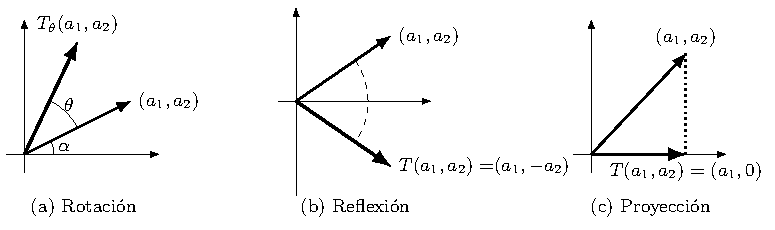
\includegraphics[width=0.85\textwidth]{figuras/rotacion-reflexion-proyeccion.pdf}
        \caption{Rotación, reflexión y proyección en $\R^2$.}
    \end{figure}

    Ahora consideramos algunos ejemplos adicionales de transformaciones lineales.

    \begin{ejemplo}
        Definamos $T:M_{m\times n}(F)\to M_{n\times m}(F)$ por $T(A)=A^t$, la transpuesta de $A$, definida en la Sección~1.3. Entonces $T$ es una transformación lineal por el Ejercicio~32 de la Sección~1.3.
    \end{ejemplo}

    \begin{ejemplo}
        Definamos $T:P_n(\R)\to P_{n-1}(\R)$ por $T\big(f(x)\big)=f'(x)$, donde $f'(x)$ denota la derivada de $f(x)$. Para mostrar que $T$ es lineal, sean $g(x),h(x)\in P_n(\R)$ y $a\in\R$. Entonces
        \begin{equation*}
            T\big(ag(x)+h(x)\big)=\big(ag(x)+h(x)\big)'=ag'(x)+h'(x)=aT\big(g(x)\big)+T\big(h(x)\big).
        \end{equation*}
        Así, por la propiedad 2 anterior, $T$ es lineal.
    \end{ejemplo}

    \begin{ejemplo}
        Sea $V=C(\R)$, el espacio vectorial de las funciones continuas de valores reales sobre $\R$. Sean $a,b\in\R$, $a<b$. Definamos $T:V\to\R$ por
        \begin{equation*}
            T(f)=\int_a^bf(t)\,dt
        \end{equation*}
        para toda $f\in V$. Entonces $T$ es una transformación lineal porque la integral definida de una combinación lineal de funciones es igual a la combinación lineal de las integrales definidas de las funciones.
    \end{ejemplo}

    Dos ejemplos muy importantes de transformaciones lineales que aparecen con frecuencia en el resto de estas notas, y que por tanto merecen su propia notación, son la identidad y la transformación cero.

    Para espacios vectoriales $V$ y $W$ (sobre $F$), definimos la \textbf{transformación identidad} $I_V:V\to V$ por $I_V(x)=x$ para todo $x\in V$, y la \textbf{transformación cero} $T_0:V\to W$ por $T_0(x)=0$ para todo $x\in V$. Es claro que ambas transformaciones son lineales. Frecuentemente escribimos $I$ en lugar de $I_V$.

    Dirigimos ahora nuestra atención a dos conjuntos muy importantes asociados con las transformaciones lineales: el \textit{rango} y el \textit{espacio nulo}. La determinación de estos conjuntos nos permite examinar más de cerca las propiedades intrínsecas de una transformación lineal.

    \begin{definicion}[Espacio nulo y rango]
        Sean $V$ y $W$ espacios vectoriales, y sea $T:V\to W$ lineal. Definimos el \textbf{espacio nulo} (o \textbf{núcleo}) $\ker(T)$ de $T$ como el conjunto de todos los vectores $x$ en $V$ tales que $T(x)=0$; es decir, $\ker(T)=\{x\in V:T(x)=0\}$.

        Definimos el \textbf{rango} (o \textbf{imagen}) $\Im(T)$ de $T$ como el subconjunto de $W$ que consiste de todas las imágenes (bajo $T$) de vectores de $V$; es decir, $\Im(T)=\{T(x):x\in V\}$.
    \end{definicion}

    \begin{ejemplo}
        Sean $V$ y $W$ espacios vectoriales, y sean $I:V\to V$ y $T_0:V\to W$ las transformaciones identidad y cero, respectivamente. Entonces $\ker(I)=\{0\}$, $\Im(I)=V$, $\ker(T_0)=V$, y $\Im(T_0)=\{0\}$.
    \end{ejemplo}

    \begin{ejemplo}
        Sea $T:\R^3\to\R^2$ la transformación lineal definida por
        \begin{equation*}
            T(a_1,a_2,a_3)=(a_1-a_2,\,2a_3).
        \end{equation*}
        Verificamos que
        \begin{equation*}
            \ker(T)=\{(a,a,0):a\in\R\} \qquad\text{y}\qquad \Im(T)=\R^2.
        \end{equation*}
        En efecto, $(a_1,a_2,a_3)\in\ker(T)$ si y solo si $a_1-a_2=0$ y $2a_3=0$, es decir, si y solo si $a_1=a_2$ y $a_3=0$; esto prueba la primera igualdad. Para la segunda, dado cualquier $(b_1,b_2)\in\R^2$, tomando $a_1=b_1$, $a_2=0$, $a_3=b_2/2$ tenemos $T(a_1,a_2,a_3)=(b_1,b_2)$; así $\Im(T)=\R^2$.
    \end{ejemplo}

    En los ejemplos anteriores, vemos que el rango y el espacio nulo de cada una de las transformaciones lineales es un subespacio. El siguiente resultado muestra que esto es cierto en general.

    \begin{teorema}
        Sean $V$ y $W$ espacios vectoriales, y sea $T:V\to W$ lineal. Entonces $\ker(T)$ y $\Im(T)$ son subespacios de $V$ y de $W$, respectivamente.
    \end{teorema}

    \begin{proof}
        Como $T(0)=0$, tenemos $0\in\ker(T)$. Sean $x,y\in\ker(T)$ y $c\in F$. Entonces $T(x+y)=T(x)+T(y)=0+0=0$, y $T(cx)=cT(x)=c0=0$. Así $x+y\in\ker(T)$ y $cx\in\ker(T)$, de modo que $\ker(T)$ es un subespacio de $V$.

        Como $T(0)=0$, tenemos $0\in\Im(T)$. Sean ahora $x,y\in\Im(T)$ y $c\in F$. Entonces existen $v,w\in V$ tales que $T(v)=x$ y $T(w)=y$. Así $T(v+w)=T(v)+T(w)=x+y$ y $T(cv)=cT(v)=cx$. Por tanto $x+y\in\Im(T)$ y $cx\in\Im(T)$, así que $\Im(T)$ es un subespacio de $W$.
    \end{proof}

    El siguiente teorema proporciona un método para encontrar un conjunto generador para el rango de una transformación lineal. Con esto logrado, una base para el rango es fácil de encontrar usando la técnica del Ejemplo~29 de la Sección~1.6.

    \begin{teorema}
        Sean $V$ y $W$ espacios vectoriales, y sea $T:V\to W$ lineal. Si $\BB=\{v_1,v_2,\dots,v_n\}$ es una base para $V$, entonces
        \begin{equation*}
            \Im(T)=\gen{T(\BB)}=\gen{\{T(v_1),T(v_2),\dots,T(v_n)\}}.
        \end{equation*}
    \end{teorema}

    \begin{proof}
        Claramente $T(v_i)\in\Im(T)$ para cada $i$. Como $\Im(T)$ es un subespacio, $\Im(T)$ contiene $\gen{\{T(v_1),T(v_2),\dots,T(v_n)\}}=\gen{T(\BB)}$ por el Teorema~1.5.

        Supongamos ahora que $w\in\Im(T)$. Entonces $w=T(v)$ para algún $v\in V$. Como $\BB$ es una base para $V$, tenemos
        \begin{equation*}
            v=\sum_{i=1}^{n}a_iv_i \qquad\text{para algunos }a_1,a_2,\dots,a_n\in F.
        \end{equation*}
        Como $T$ es lineal, se sigue que
        \begin{equation*}
            w=T(v)=\sum_{i=1}^{n}a_iT(v_i)\in\gen{T(\BB)}.
        \end{equation*}
        Así $\Im(T)$ está contenido en $\gen{T(\BB)}$.
    \end{proof}

    Debe notarse que el teorema anterior es válido incluso si $\BB$ es infinita, es decir, $\Im(T)=\gen{\{T(v):v\in\BB\}}$ (véase el Ejercicio~34).

    El siguiente ejemplo ilustra la utilidad del teorema anterior.

    \begin{ejemplo}
        Definamos la transformación lineal $T:P_2(\R)\to M_{2\times 2}(\R)$ por
        \begin{equation*}
            T\big(f(x)\big)=\begin{pmatrix}f(1)-f(2)&0\\0&f(0)\end{pmatrix}.
        \end{equation*}
        Como $\BB=\{1,x,x^2\}$ es una base para $P_2(\R)$, tenemos
        \begin{align*}
            \Im(T)&=\gen{T(\BB)}=\gen{\{T(1),T(x),T(x^2)\}}\\
            &=\gen{\left\{\begin{pmatrix}0&0\\0&1\end{pmatrix},\begin{pmatrix}-1&0\\0&0\end{pmatrix},\begin{pmatrix}-3&0\\0&0\end{pmatrix}\right\}}\\
            &=\gen{\left\{\begin{pmatrix}0&0\\0&1\end{pmatrix},\begin{pmatrix}-1&0\\0&0\end{pmatrix}\right\}}.
        \end{align*}
        Así hemos encontrado una base para $\Im(T)$, y por tanto $\dim\big(\Im(T)\big)=2$.
    \end{ejemplo}

    Como en el Capítulo~1, medimos el \textquotedblleft tamaño\textquotedblright\ de un subespacio por su dimensión. El espacio nulo y el rango son tan importantes que asignamos nombres especiales a sus respectivas dimensiones.

    \begin{definicion}[Nulidad y rango]
        Sean $V$ y $W$ espacios vectoriales, y sea $T:V\to W$ lineal. Si $\ker(T)$ y $\Im(T)$ son de dimensión finita, definimos la \textbf{nulidad} de $T$, denotada $\nul(T)$, y el \textbf{rango} de $T$, denotado $\rg(T)$, como las dimensiones de $\ker(T)$ y de $\Im(T)$, respectivamente.
    \end{definicion}

    Reflexionando sobre la acción de una transformación lineal, vemos intuitivamente que cuanto mayor sea la nulidad, menor será el rango. En otras palabras, cuantos más vectores sean enviados a $0$, más pequeño será el rango. El mismo razonamiento heurístico nos dice que, cuanto mayor sea el rango, menor será la nulidad. Este equilibrio entre rango y nulidad se precisa en el siguiente teorema, apropiadamente llamado el \textit{teorema de la dimensión}.

    \begin{teorema}[Teorema de la dimensión]
        Sean $V$ y $W$ espacios vectoriales, y sea $T:V\to W$ lineal. Si $V$ es de dimensión finita, entonces
        \begin{equation*}
            \nul(T)+\rg(T)=\dim(V).
        \end{equation*}
    \end{teorema}

    \begin{proof}
        Supongamos que $\dim(V)=n$, $\dim\big(\ker(T)\big)=k$, y que $\{v_1,v_2,\dots,v_k\}$ es una base para $\ker(T)$. Por el corolario al Teorema~1.11, podemos extender $\{v_1,v_2,\dots,v_k\}$ a una base $\BB=\{v_1,v_2,\dots,v_n\}$ para $V$. Afirmamos que $S=\{T(v_{k+1}),T(v_{k+2}),\dots,T(v_n)\}$ es una base para $\Im(T)$.

        Primero probamos que $S$ genera a $\Im(T)$. Usando el teorema anterior y el hecho de que $T(v_i)=0$ para $1\leq i\leq k$, tenemos
        \begin{align*}
            \Im(T)&=\gen{\{T(v_1),T(v_2),\dots,T(v_n)\}}\\
            &=\gen{\{T(v_{k+1}),T(v_{k+2}),\dots,T(v_n)\}}=\gen{S}.
        \end{align*}

        Ahora probamos que $S$ es linealmente independiente. Supongamos que
        \begin{equation*}
            \sum_{i=k+1}^{n}b_iT(v_i)=0 \qquad\text{para }b_{k+1},b_{k+2},\dots,b_n\in F.
        \end{equation*}
        Usando el hecho de que $T$ es lineal, tenemos
        \begin{equation*}
            T\left(\sum_{i=k+1}^{n}b_iv_i\right)=0.
        \end{equation*}
        Así
        \begin{equation*}
            \sum_{i=k+1}^{n}b_iv_i\in\ker(T).
        \end{equation*}
        Por tanto existen $c_1,c_2,\dots,c_k\in F$ tales que
        \begin{equation*}
            \sum_{i=k+1}^{n}b_iv_i=\sum_{i=1}^{k}c_iv_i \qquad\text{o}\qquad \sum_{i=1}^{k}(-c_i)v_i+\sum_{i=k+1}^{n}b_iv_i=0.
        \end{equation*}
        Como $\BB$ es una base para $V$, tenemos $b_i=0$ para toda $i$. Por tanto $S$ es linealmente independiente. Notemos que este argumento también muestra que $T(v_{k+1}),T(v_{k+2}),\dots,T(v_n)$ son distintos; por tanto $\rg(T)=n-k$.
    \end{proof}

    Si aplicamos el teorema de la dimensión al ejemplo anterior de $T:\R^3\to\R^2$, $T(a_1,a_2,a_3)=(a_1-a_2,2a_3)$, tenemos que $\nul(T)+2=3$, así que $\nul(T)=1$; en efecto, ya vimos que $\ker(T)=\{(a,a,0):a\in\R\}$, un subespacio de dimensión $1$.

    El lector debe repasar los conceptos de \textquotedblleft inyectiva\textquotedblright\ (uno a uno) y \textquotedblleft sobreyectiva\textquotedblright\ (sobre). Recordemos que una función $T:V\to W$ es \textbf{inyectiva} si $T(x)=T(y)$ implica $x=y$ (equivalentemente, elementos distintos de $V$ tienen imágenes distintas bajo $T$), y es \textbf{sobreyectiva} si $\Im(T)=W$. Curiosamente, para una transformación lineal, ambos conceptos están íntimamente conectados con el rango y la nulidad de la transformación. Esto se demuestra en los siguientes dos teoremas.

    \begin{teorema}
        Sean $V$ y $W$ espacios vectoriales, y sea $T:V\to W$ lineal. Entonces $T$ es inyectiva si y solo si $\ker(T)=\{0\}$.
    \end{teorema}

    \begin{proof}
        Supongamos que $T$ es inyectiva y sea $x\in\ker(T)$. Entonces $T(x)=0=T(0)$. Como $T$ es inyectiva, tenemos $x=0$. Por tanto $\ker(T)=\{0\}$.

        Supongamos ahora que $\ker(T)=\{0\}$, y sean $x,y\in V$ tales que $T(x)=T(y)$. Entonces $0=T(x)-T(y)=T(x-y)$ por la propiedad~3 anterior. Por tanto $x-y\in\ker(T)=\{0\}$. Esto significa que $x-y=0$, o $x=y$. Así $T$ es inyectiva.
    \end{proof}

    El lector debe observar que el Teorema~2.4 nos permite concluir que la transformación definida en el Ejemplo~9 no es inyectiva.

    Sorprendentemente, las condiciones de inyectividad y sobreyectividad son equivalentes en un caso especial importante.

    \begin{teorema}
        Sean $V$ y $W$ espacios vectoriales de igual dimensión (finita), y sea $T:V\to W$ lineal. Entonces las siguientes afirmaciones son equivalentes:
        \begin{enumerate}[label=(\alph*)]
            \item $T$ es inyectiva.
            \item $T$ es sobreyectiva.
            \item $\rg(T)=\dim(V)$.
        \end{enumerate}
    \end{teorema}

    \begin{proof}
        Por el teorema de la dimensión, tenemos
        \begin{equation*}
            \nul(T)+\rg(T)=\dim(V).
        \end{equation*}
        Ahora, usando el Teorema~2.4, tenemos que $T$ es inyectiva si y solo si $\ker(T)=\{0\}$, si y solo si $\nul(T)=0$, si y solo si $\rg(T)=\dim(V)$, si y solo si $\rg(T)=\dim(W)$, y si y solo si $\dim\big(\Im(T)\big)=\dim(W)$. Por el Teorema~1.11, esta igualdad es equivalente a $\Im(T)=W$, la definición de que $T$ sea sobreyectiva.
    \end{proof}

    Observemos que, si $V$ no es de dimensión finita y $T:V\to V$ es lineal, entonces \textit{no} se sigue que la inyectividad y la sobreyectividad sean equivalentes. (Véanse los Ejercicios~15, 16 y 21.)

    La linealidad de $T$ en los Teoremas~2.4 y 2.5 es esencial, pues es fácil construir ejemplos de funciones de $\R$ en $\R$ que no son inyectivas, pero sí sobreyectivas, y viceversa.

    Los siguientes dos ejemplos hacen uso de los teoremas anteriores para determinar si una transformación lineal dada es inyectiva o sobreyectiva.

    \begin{ejemplo}
        Sea $T:P_2(\R)\to P_3(\R)$ la transformación lineal definida por
        \begin{equation*}
            T\big(f(x)\big)=2f'(x)+\int_0^x3f(t)\,dt.
        \end{equation*}
        Ahora
        \begin{equation*}
            \Im(T)=\gen{\{T(1),T(x),T(x^2)\}}=\gen{\left\{3x,\;2+\tfrac32x^2,\;4x+x^3\right\}}.
        \end{equation*}
        Como $\{3x,2+\frac32x^2,4x+x^3\}$ es linealmente independiente, $\rg(T)=3$. Como $\dim\big(P_3(\R)\big)=4$, $T$ no es sobreyectiva. Por el teorema de la dimensión, $\nul(T)+3=3$. Así $\nul(T)=0$, y por tanto $\ker(T)=\{0\}$. Concluimos, por el Teorema~2.4, que $T$ es inyectiva.
    \end{ejemplo}

    \begin{ejemplo}
        Sea $T:F^2\to F^2$ la transformación lineal definida por
        \begin{equation*}
            T(a_1,a_2)=(a_1+a_2,\,a_1).
        \end{equation*}
        Es fácil ver que $\ker(T)=\{0\}$; así $T$ es inyectiva. Por tanto el Teorema~2.5 nos dice que $T$ debe ser sobreyectiva.
    \end{ejemplo}

    En el Ejercicio~15 se establece que, si $T$ es lineal e inyectiva, entonces un subconjunto $S$ es linealmente independiente si y solo si $T(S)$ es linealmente independiente. El siguiente ejemplo ilustra el uso de este resultado.

    \begin{ejemplo}
        Sea $T:P_2(\R)\to\R^3$ la transformación lineal definida por
        \begin{equation*}
            T(a_0+a_1x+a_2x^2)=(a_0,a_1,a_2).
        \end{equation*}
        Claramente $T$ es lineal e inyectiva. Sea $S=\{2-x+3x^2,\,x+x^2,\,1-2x^2\}$. Entonces $S$ es linealmente independiente en $P_2(\R)$ porque
        \begin{equation*}
            T(S)=\{(2,-1,3),(0,1,1),(1,0,-2)\}
        \end{equation*}
        es linealmente independiente en $\R^3$.
    \end{ejemplo}

    En el ejemplo anterior, transferimos una propiedad del espacio vectorial de polinomios a una propiedad del espacio vectorial de $3$-adas. Esta técnica se explota más ampliamente más adelante.

    Una de las propiedades más importantes de una transformación lineal es que queda completamente determinada por su acción sobre una base. Este resultado, que se sigue del siguiente teorema y su corolario, se usa con frecuencia a lo largo de estas notas.

    \begin{teorema}
        Sean $V$ y $W$ espacios vectoriales sobre $F$, y supongamos que $\{v_1,v_2,\dots,v_n\}$ es una base para $V$. Para $w_1,w_2,\dots,w_n$ en $W$, existe exactamente una transformación lineal $T:V\to W$ tal que $T(v_i)=w_i$ para $i=1,2,\dots,n$.
    \end{teorema}

    \begin{proof}
        Sea $x\in V$. Entonces
        \begin{equation*}
            x=\sum_{i=1}^{n}a_iv_i,
        \end{equation*}
        donde $a_1,a_2,\dots,a_n$ son escalares únicos. Definamos
        \begin{equation*}
            T:V\to W \qquad\text{por}\qquad T(x)=\sum_{i=1}^{n}a_iw_i.
        \end{equation*}

        (a) $T$ es lineal: Supongamos que $u,v\in V$ y $d\in F$. Entonces podemos escribir
        \begin{equation*}
            u=\sum_{i=1}^{n}b_iv_i \qquad\text{y}\qquad v=\sum_{i=1}^{n}c_iv_i
        \end{equation*}
        para algunos escalares $b_1,b_2,\dots,b_n,c_1,c_2,\dots,c_n$. Así
        \begin{equation*}
            du+v=\sum_{i=1}^{n}(db_i+c_i)v_i.
        \end{equation*}
        Por tanto
        \begin{equation*}
            T(du+v)=\sum_{i=1}^{n}(db_i+c_i)w_i=d\sum_{i=1}^{n}b_iw_i+\sum_{i=1}^{n}c_iw_i=dT(u)+T(v).
        \end{equation*}

        (b) Claramente $T(v_i)=w_i$ para $i=1,2,\dots,n$.

        (c) $T$ es única: Supongamos que $U:V\to W$ es lineal y $U(v_i)=w_i$ para $i=1,2,\dots,n$. Entonces, para $x\in V$ con
        \begin{equation*}
            x=\sum_{i=1}^{n}a_iv_i,
        \end{equation*}
        tenemos
        \begin{equation*}
            U(x)=\sum_{i=1}^{n}a_iU(v_i)=\sum_{i=1}^{n}a_iw_i=T(x).
        \end{equation*}
        Por tanto $U=T$.
    \end{proof}

    \begin{corolario}
        Sean $V$ y $W$ espacios vectoriales, y supongamos que $V$ tiene una base finita $\{v_1,v_2,\dots,v_n\}$. Si $U,T:V\to W$ son lineales y $U(v_i)=T(v_i)$ para $i=1,2,\dots,n$, entonces $U=T$.
    \end{corolario}

    \begin{proof}
        Se sigue inmediatamente de la unicidad probada en el teorema anterior, aplicado con $w_i=T(v_i)=U(v_i)$ para cada $i$.
    \end{proof}

    \begin{ejemplo}
        Sea $T:\R^2\to\R^2$ la transformación lineal definida por
        \begin{equation*}
            T(a_1,a_2)=(2a_2-a_1,\,3a_1),
        \end{equation*}
        y supongamos que $U:\R^2\to\R^2$ es lineal. Si sabemos que $U(1,2)=(3,3)$ y $U(1,1)=(1,3)$, entonces $U=T$. Esto se sigue del corolario anterior y del hecho de que $\{(1,2),(1,1)\}$ es una base para $\R^2$.
    \end{ejemplo}

    \begin{ejercicio}
        Etiquete las siguientes afirmaciones como verdaderas o falsas. En cada inciso, $V$ y $W$ son espacios vectoriales de dimensión finita (sobre $F$), y $T$ es una función de $V$ en $W$.
        \begin{enumerate}[label=(\alph*)]
            \item Si $T$ es lineal, entonces $T$ preserva sumas y productos por escalares.
            \item Si $T(x+y)=T(x)+T(y)$, entonces $T$ es lineal.
            \item $T$ es inyectiva si y solo si el único vector $x$ tal que $T(x)=0$ es $x=0$.
            \item Si $T$ es lineal, entonces $T(0_V)=0_W$.
            \item Si $T$ es lineal, entonces $\nul(T)+\rg(T)=\dim(W)$.
            \item Si $T$ es lineal, entonces $T$ lleva subconjuntos linealmente independientes de $V$ en subconjuntos linealmente independientes de $W$.
            \item Si $T,U:V\to W$ son ambas lineales y coinciden en una base de $V$, entonces $T=U$.
            \item Dados $x_1,x_2\in V$ y $y_1,y_2\in W$, existe una transformación lineal $T:V\to W$ tal que $T(x_1)=y_1$ y $T(x_2)=y_2$.
        \end{enumerate}
    \end{ejercicio}

    \begin{ejercicio}
        Para los Ejercicios 2 al 6, pruebe que $T$ es una transformación lineal, y encuentre bases tanto para $\ker(T)$ como para $\Im(T)$. Después calcule la nulidad y el rango de $T$, y verifique el teorema de la dimensión. Finalmente, use los teoremas apropiados de esta sección para determinar si $T$ es inyectiva o sobreyectiva.
    \end{ejercicio}

    \begin{ejercicio}
        $T:\R^3\to\R^2$ definida por $T(a_1,a_2,a_3)=(a_1-a_2,\,2a_3)$.
    \end{ejercicio}

    \begin{ejercicio}
        $T:\R^2\to\R^3$ definida por $T(a_1,a_2)=(a_1+a_2,\,0,\,2a_1-a_2)$.
    \end{ejercicio}

    \begin{ejercicio}
        $T:M_{2\times 3}(F)\to M_{2\times 2}(F)$ definida por
        \begin{equation*}
            T\begin{pmatrix}a_{11}&a_{12}&a_{13}\\a_{21}&a_{22}&a_{23}\end{pmatrix}=\begin{pmatrix}2a_{11}-a_{12}&a_{13}+2a_{12}\\0&0\end{pmatrix}.
        \end{equation*}
    \end{ejercicio}

    \begin{ejercicio}
        $T:P_2(\R)\to P_3(\R)$ definida por $T\big(f(x)\big)=xf(x)+f'(x)$.
    \end{ejercicio}

    \begin{ejercicio}
        $T:M_{n\times n}(F)\to F$ definida por $T(A)=\Tr(A)$. Recordemos (Ejemplo~4, Sección~1.3) que
        \begin{equation*}
            \Tr(A)=\sum_{i=1}^{n}A_{ii}.
        \end{equation*}
    \end{ejercicio}

    \begin{ejercicio}
        Pruebe las propiedades 1, 2, 3 y 4 enunciadas al principio de esta sección.
    \end{ejercicio}

    \begin{ejercicio}
        Pruebe que las transformaciones de los Ejemplos~3 y 4 (la reflexión y la proyección) son lineales.
    \end{ejercicio}

    \begin{ejercicio}
        En este ejercicio, $T:\R^2\to\R^2$ es una función. Para cada uno de los siguientes incisos, indique por qué $T$ \textit{no} es lineal.
        \begin{enumerate}[label=(\alph*)]
            \item $T(a_1,a_2)=(1,a_2)$
            \item $T(a_1,a_2)=(a_1,a_1^2)$
            \item $T(a_1,a_2)=(\sin a_1,0)$
            \item $T(a_1,a_2)=(|a_1|,a_2)$
            \item $T(a_1,a_2)=(a_1+1,a_2)$
        \end{enumerate}
    \end{ejercicio}

    \begin{ejercicio}
        Supongamos que $T:\R^2\to\R^2$ es lineal, $T(1,0)=(1,4)$, y $T(1,1)=(2,5)$. ¿Cuánto es $T(2,3)$? ¿Es $T$ inyectiva?
    \end{ejercicio}

    \begin{ejercicio}
        Pruebe que existe una transformación lineal $T:\R^2\to\R^3$ tal que $T(1,1)=(1,0,2)$ y $T(2,3)=(1,-1,4)$. ¿Cuánto es $T(8,11)$?
    \end{ejercicio}

    \begin{ejercicio}
        ¿Existe una transformación lineal $T:\R^3\to\R^2$ tal que $T(1,0,3)=(1,1)$ y $T(-2,0,-6)=(2,1)$?
    \end{ejercicio}

    \begin{ejercicio}
        Sean $V$ y $W$ espacios vectoriales, sea $T:V\to W$ lineal, y sea $\{w_1,w_2,\dots,w_k\}$ un subconjunto linealmente independiente de $\Im(T)$. Pruebe que, si $S=\{v_1,v_2,\dots,v_k\}$ se elige de modo que $T(v_i)=w_i$ para $i=1,2,\dots,k$, entonces $S$ es linealmente independiente.
    \end{ejercicio}

    \begin{ejercicio}
        Sean $V$ y $W$ espacios vectoriales y $T:V\to W$ lineal.
        \begin{enumerate}[label=(\alph*)]
            \item Pruebe que $T$ es inyectiva si y solo si $T$ lleva subconjuntos linealmente independientes de $V$ en subconjuntos linealmente independientes de $W$.
            \item Supongamos que $T$ es inyectiva y que $S$ es un subconjunto de $V$. Pruebe que $S$ es linealmente independiente si y solo si $T(S)$ es linealmente independiente.
            \item Supongamos que $\BB=\{v_1,v_2,\dots,v_n\}$ es una base para $V$ y que $T$ es inyectiva y sobreyectiva. Pruebe que $T(\BB)=\{T(v_1),T(v_2),\dots,T(v_n)\}$ es una base para $W$.
        \end{enumerate}
    \end{ejercicio}

    \begin{ejercicio}
        Recordemos la definición de $P(\R)$ dada en la Sección~1.2. Definamos
        \begin{equation*}
            T:P(\R)\to P(\R) \qquad\text{por}\qquad T\big(f(x)\big)=\int_0^xf(t)\,dt.
        \end{equation*}
        Pruebe que $T$ es lineal e inyectiva, pero no sobreyectiva.
    \end{ejercicio}

    \begin{ejercicio}
        Sea $T:P(\R)\to P(\R)$ definida por $T\big(f(x)\big)=f'(x)$. Recordemos que $T$ es lineal. Pruebe que $T$ es sobreyectiva, pero no inyectiva.
    \end{ejercicio}

    \begin{ejercicio}
        Sean $V$ y $W$ espacios vectoriales de dimensión finita, y sea $T:V\to W$ lineal.
        \begin{enumerate}[label=(\alph*)]
            \item Pruebe que, si $\dim(V)<\dim(W)$, entonces $T$ no puede ser sobreyectiva.
            \item Pruebe que, si $\dim(V)>\dim(W)$, entonces $T$ no puede ser inyectiva.
        \end{enumerate}
    \end{ejercicio}

    \begin{ejercicio}
        Dé un ejemplo de una transformación lineal $T:\R^2\to\R^2$ tal que $\ker(T)=\Im(T)$.
    \end{ejercicio}

    \begin{ejercicio}
        Dé un ejemplo de transformaciones lineales distintas $T$ y $U$ tales que $\ker(T)=\ker(U)$ y $\Im(T)=\Im(U)$.
    \end{ejercicio}

    \begin{ejercicio}
        Sean $V$ y $W$ espacios vectoriales con subespacios $V_1$ y $W_1$, respectivamente. Si $T:V\to W$ es lineal, pruebe que $T(V_1)$ es un subespacio de $W$ y que $\{x\in V:T(x)\in W_1\}$ es un subespacio de $V$.
    \end{ejercicio}

    \begin{ejercicio}
        Sea $V$ el espacio vectorial de las sucesiones descrito en el Ejemplo~7 de la Sección~1.2. Definamos las funciones $T,U:V\to V$ por
        \begin{equation*}
            T(a_1,a_2,\dots)=(a_2,a_3,\dots) \qquad\text{y}\qquad U(a_1,a_2,\dots)=(0,a_1,a_2,\dots).
        \end{equation*}
        A $T$ y a $U$ se les llama los operadores de \textbf{desplazamiento a la izquierda} y \textbf{desplazamiento a la derecha} sobre $V$, respectivamente.
        \begin{enumerate}[label=(\alph*)]
            \item Pruebe que $T$ y $U$ son lineales.
            \item Pruebe que $T$ es sobreyectiva, pero no inyectiva.
            \item Pruebe que $U$ es inyectiva, pero no sobreyectiva.
        \end{enumerate}
    \end{ejercicio}

    \begin{ejercicio}
        Sea $T:\R^3\to\R$ lineal. Muestre que existen escalares $a$, $b$ y $c$ tales que $T(x,y,z)=ax+by+cz$ para todo $(x,y,z)\in\R^3$. ¿Puede generalizar este resultado para $T:F^n\to F$? Enuncie y pruebe un resultado análogo para $T:F^n\to F^m$.
    \end{ejercicio}

    \begin{ejercicio}
        Sea $T:\R^3\to\R$ lineal. Describa geométricamente las posibilidades para el espacio nulo de $T$. \textit{Sugerencia:} Use el ejercicio anterior.
    \end{ejercicio}

    La siguiente definición se usa en los Ejercicios~24 a 27 y en el Ejercicio~30.

    \begin{definicion}[Proyección sobre un subespacio a lo largo de otro]
        Sean $V$ un espacio vectorial y $W_1$ y $W_2$ subespacios de $V$ tales que $V=W_1\oplus W_2$. (Recordemos la definición de suma directa dada en los ejercicios de la Sección~1.3.) Una función $T:V\to V$ se llama la \textbf{proyección sobre $W_1$ a lo largo de $W_2$} si, para $x=x_1+x_2$ con $x_1\in W_1$ y $x_2\in W_2$, tenemos $T(x)=x_1$.
    \end{definicion}

    \begin{ejercicio}
        Sea $T:\R^2\to\R^2$. Incluya figuras para cada uno de los siguientes incisos.
        \begin{enumerate}[label=(\alph*)]
            \item Encuentre una fórmula para $T(a,b)$, donde $T$ representa la proyección sobre el eje $y$ a lo largo del eje $x$.
            \item Encuentre una fórmula para $T(a,b)$, donde $T$ representa la proyección sobre el eje $y$ a lo largo de la recta $L=\{(s,s):s\in\R\}$.
        \end{enumerate}
    \end{ejercicio}

    \begin{ejercicio}
        Sea $T:\R^3\to\R^3$.
        \begin{enumerate}[label=(\alph*)]
            \item Si $T(a,b,c)=(a,b,0)$, muestre que $T$ es la proyección sobre el plano $xy$ a lo largo del eje $z$.
            \item Encuentre una fórmula para $T(a,b,c)$, donde $T$ representa la proyección sobre el eje $z$ a lo largo del plano $xy$.
            \item Si $T(a,b,c)=(a-c,b,0)$, muestre que $T$ es la proyección sobre el plano $xy$ a lo largo de la recta $L=\{(a,0,a):a\in\R\}$.
        \end{enumerate}
    \end{ejercicio}

    \begin{ejercicio}
        Usando la notación de la definición anterior, supongamos que $T:V\to V$ es la proyección sobre $W_1$ a lo largo de $W_2$.
        \begin{enumerate}[label=(\alph*)]
            \item Pruebe que $T$ es lineal y que $W_1=\{x\in V:T(x)=x\}$.
            \item Pruebe que $W_1=\Im(T)$ y $W_2=\ker(T)$.
            \item Describa $T$ si $W_1=V$.
            \item Describa $T$ si $W_1$ es el subespacio cero.
        \end{enumerate}
    \end{ejercicio}

    \begin{ejercicio}
        Supongamos que $W$ es un subespacio de un espacio vectorial de dimensión finita $V$.
        \begin{enumerate}[label=(\alph*)]
            \item Pruebe que existe un subespacio $W'$ y una función $T:V\to V$ tales que $T$ es la proyección sobre $W$ a lo largo de $W'$.
            \item Dé un ejemplo de un subespacio $W$ de un espacio vectorial $V$ tal que existan \textit{dos} proyecciones sobre $W$ a lo largo de dos subespacios (distintos).
        \end{enumerate}
    \end{ejercicio}

    Las siguientes definiciones se usan en los Ejercicios~28 a 32. Sea $V$ un espacio vectorial, y sea $T:V\to V$ lineal. Un subespacio $W$ de $V$ se dice \textbf{$T$-invariante} si $T(W)\subseteq W$, es decir, si $T(x)\in W$ para todo $x\in W$. Si $W$ es $T$-invariante, definimos la \textbf{restricción de $T$ sobre $W$} como la función $T_W:W\to W$ definida por $T_W(x)=T(x)$ para todo $x\in W$.

    Los Ejercicios~28 a 32 suponen que $W$ es un subespacio de un espacio vectorial $V$ y que $T:V\to V$ es lineal. \textit{Advertencia:} no suponga que $W$ es $T$-invariante ni que $T$ es una proyección a menos que se indique explícitamente.

    \begin{ejercicio}
        Pruebe que los subespacios $\{0\}$, $V$, $\Im(T)$, y $\ker(T)$ son todos $T$-invariantes.
    \end{ejercicio}

    \begin{ejercicio}
        Si $W$ es $T$-invariante, pruebe que $T_W$ es lineal.
    \end{ejercicio}

    \begin{ejercicio}
        Supongamos que $T$ es la proyección sobre $W$ a lo largo de algún subespacio $W'$. Pruebe que $W$ es $T$-invariante y que $T_W=I_W$.
    \end{ejercicio}

    \begin{ejercicio}
        Supongamos que $V=\Im(T)\oplus W$ y que $W$ es $T$-invariante. (Recordemos la definición de suma directa dada en los ejercicios de la Sección~1.3.)
        \begin{enumerate}[label=(\alph*)]
            \item Pruebe que $W\subseteq\ker(T)$.
            \item Muestre que, si $V$ es de dimensión finita, entonces $W=\ker(T)$.
            \item Muestre, mediante un ejemplo, que la conclusión de (b) no es necesariamente cierta si $V$ no es de dimensión finita.
        \end{enumerate}
    \end{ejercicio}

    \begin{ejercicio}
        Supongamos que $W$ es $T$-invariante. Pruebe que $\ker(T_W)=\ker(T)\cap W$ y $\Im(T_W)=T(W)$.
    \end{ejercicio}

    \begin{ejercicio}
        Pruebe el Teorema~2.2 para el caso en que $\BB$ es infinita, es decir, $\Im(T)=\gen{\{T(v):v\in\BB\}}$.
    \end{ejercicio}

    \begin{ejercicio}
        Pruebe la siguiente generalización del Teorema~2.6: Sean $V$ y $W$ espacios vectoriales sobre un campo común, y sea $\BB$ una base para $V$. Entonces, para cualquier función $f:\BB\to W$, existe exactamente una transformación lineal $T:V\to W$ tal que $T(x)=f(x)$ para todo $x\in\BB$.
    \end{ejercicio}

    Los Ejercicios~36 y 37 suponen la definición de suma directa dada en los ejercicios de la Sección~1.3.

    \begin{ejercicio}
        Sea $V$ un espacio vectorial de dimensión finita y $T:V\to V$ lineal.
        \begin{enumerate}[label=(\alph*)]
            \item Supongamos que $V=\Im(T)+\ker(T)$. Pruebe que $V=\Im(T)\oplus\ker(T)$.
            \item Supongamos que $\Im(T)\cap\ker(T)=\{0\}$. Pruebe que $V=\Im(T)\oplus\ker(T)$.
        \end{enumerate}
        Tenga cuidado de indicar en cada inciso dónde se usa la dimensión finita.
    \end{ejercicio}

    \begin{ejercicio}
        Sean $V$ y $T$ como en el Ejercicio~21.
        \begin{enumerate}[label=(\alph*)]
            \item Pruebe que $V=\Im(T)+\ker(T)$, pero $V$ no es la suma directa de estos dos espacios. Así el resultado del Ejercicio~36(a) no puede probarse sin suponer que $V$ es de dimensión finita.
            \item Encuentre un operador lineal $T_1$ sobre $V$ tal que $\Im(T_1)\cap\ker(T_1)=\{0\}$, pero $V$ no es la suma directa de $\Im(T_1)$ y $\ker(T_1)$. Concluya que el hecho de que $V$ sea de dimensión finita es también esencial en el Ejercicio~36(b).
        \end{enumerate}
    \end{ejercicio}

    \begin{ejercicio}
        Una función $T:V\to W$ entre espacios vectoriales $V$ y $W$ se llama \textbf{aditiva} si $T(x+y)=T(x)+T(y)$ para todos $x,y\in V$. Pruebe que, si $V$ y $W$ son espacios vectoriales sobre el campo de los números racionales, entonces cualquier función aditiva de $V$ en $W$ es una transformación lineal.
    \end{ejercicio}

    \begin{ejercicio}
        Sea $T:\C\to\C$ la función definida por $T(z)=\overline{z}$. Pruebe que $T$ es aditiva (según se definió en el Ejercicio~38), pero no lineal.
    \end{ejercicio}

    \begin{ejercicio}
        Pruebe que existe una función aditiva $T:\R\to\R$ (según se definió en el Ejercicio~38) que no es lineal. \textit{Sugerencia:} Sea $V$ el conjunto de los números reales, considerado como un espacio vectorial sobre el campo de los números racionales. Por el corolario al Teorema~1.14, $V$ tiene una base $\BB$. Sean $x$ y $y$ dos vectores distintos de $\BB$, y definamos $f:\BB\to V$ por $f(x)=y$, $f(y)=x$, y $f(z)=z$ en cualquier otro caso. Por el ejercicio anterior, existe una transformación lineal $T:V\to V$ tal que $T(u)=f(u)$ para todo $u\in\BB$. Entonces $T$ es aditiva, pero para $c=y/x$, $T(cx)\neq cT(x)$.
    \end{ejercicio}

    El siguiente ejercicio requiere familiaridad con la definición de \textit{espacio cociente} dada en el Ejercicio~60 de la Sección~1.3.

    \begin{ejercicio}
        Sea $V$ un espacio vectorial y $W$ un subespacio de $V$. Definamos la función $\eta:V\to V/W$ por $\eta(v)=v+W$ para $v\in V$.
        \begin{enumerate}[label=(\alph*)]
            \item Pruebe que $\eta$ es una transformación lineal de $V$ sobre $V/W$ y que $\ker(\eta)=W$.
            \item Supongamos que $V$ es de dimensión finita. Use el inciso (a) y el teorema de la dimensión para deducir una fórmula que relacione $\dim(V)$, $\dim(W)$, y $\dim(V/W)$.
            \item Lea la demostración del teorema de la dimensión. Compare el método de resolver (b) con el método de obtener el mismo resultado descrito en el Ejercicio~132 de la Sección~1.6.
        \end{enumerate}
    \end{ejercicio}

    \section{La representación matricial de una transformación lineal}

    \begin{definicion}[Vector de coordenadas]
        Sea $\BB=\{u_1,u_2,\dots,u_n\}$ una base ordenada para un espacio vectorial de dimensión finita $V$. Para $x\in V$, sean $a_1,a_2,\dots,a_n$ los escalares únicos tales que
        \begin{equation*}
            x=\sum_{i=1}^{n}a_iu_i.
        \end{equation*}
        Definimos el \textbf{vector de coordenadas} de $x$ relativo a $\BB$, denotado $[x]_{\BB}$, por
        \begin{equation*}
            [x]_{\BB}=\begin{pmatrix}a_1\\a_2\\\vdots\\a_n\end{pmatrix}.
        \end{equation*}
    \end{definicion}

    Notemos que $[u_i]_{\BB}=e_i$ en la definición anterior. La correspondencia $x\mapsto[x]_{\BB}$ nos proporciona una transformación lineal de $V$ a $F^n$: en efecto, si $x=\sum_ia_iu_i$ y $y=\sum_ib_iu_i$, entonces, para cualquier escalar $c$, $cx+y=\sum_i(ca_i+b_i)u_i$, así que $[cx+y]_{\BB}=(ca_1+b_1,\dots,ca_n+b_n)^t=c(a_1,\dots,a_n)^t+(b_1,\dots,b_n)^t=c[x]_{\BB}+[y]_{\BB}$; por la propiedad~2 de la Sección~2.1, esto muestra que $x\mapsto[x]_{\BB}$ es lineal. Estudiamos esta transformación con más detalle en la Sección~2.4.

    \begin{ejemplo}
        Sea $V=P_2(\R)$, y sea $\BB=\{1,x,x^2\}$ la base ordenada estándar para $V$. Si $f(x)=4+6x-7x^2$, entonces
        \begin{equation*}
            [f]_{\BB}=\begin{pmatrix}4\\6\\-7\end{pmatrix}.
        \end{equation*}
    \end{ejemplo}

    Procedamos ahora con la prometida representación matricial de una transformación lineal. Supongamos que $V$ y $W$ son espacios vectoriales de dimensión finita con bases ordenadas $\BB=\{v_1,v_2,\dots,v_n\}$ y $\gamma=\{w_1,w_2,\dots,w_m\}$, respectivamente. Sea $T:V\to W$ lineal. Entonces, para cada $j$, $1\leq j\leq n$, existen escalares únicos $a_{ij}\in F$, $1\leq i\leq m$, tales que
    \begin{equation*}
        T(v_j)=\sum_{i=1}^{m}a_{ij}w_i \qquad\text{para }1\leq j\leq n.
    \end{equation*}

    \begin{definicion}[Representación matricial]
        Usando la notación anterior, llamamos a la matriz $A$ de tamaño $m\times n$ definida por $A_{ij}=a_{ij}$ la \textbf{representación matricial de $T$} en las bases ordenadas $\BB$ y $\gamma$, y escribimos $A=[T]_{\BB}^{\gamma}$. Si $V=W$ y $\BB=\gamma$, escribimos $A=[T]_{\BB}$.
    \end{definicion}

    Notemos que la $j$-ésima columna de $A$ es simplemente $[T(v_j)]_\gamma$. Observemos también que, si $U:V\to W$ es una transformación lineal tal que $[U]_{\BB}^\gamma=[T]_{\BB}^\gamma$, entonces $U=T$ por el corolario al Teorema~2.6. Ilustramos el cálculo de $[T]_{\BB}^\gamma$ en los siguientes ejemplos.

    \begin{ejemplo}
        Sea $T:\R^2\to\R^3$ la transformación lineal definida por
        \begin{equation*}
            T(a_1,a_2)=(a_1+3a_2,\,0,\,2a_1-4a_2).
        \end{equation*}
        Sean $\BB$ y $\gamma$ las bases ordenadas estándar para $\R^2$ y $\R^3$, respectivamente. Ahora
        \begin{equation*}
            T(1,0)=(1,0,2)=1e_1+0e_2+2e_3
        \end{equation*}
        y
        \begin{equation*}
            T(0,1)=(3,0,-4)=3e_1+0e_2-4e_3.
        \end{equation*}
        Así
        \begin{equation*}
            [T]_{\BB}^\gamma=\begin{pmatrix}1&3\\0&0\\2&-4\end{pmatrix}.
        \end{equation*}
        Si tomamos $\gamma'=\{e_3,e_2,e_1\}$, entonces
        \begin{equation*}
            [T]_{\BB}^{\gamma'}=\begin{pmatrix}2&-4\\0&0\\1&3\end{pmatrix}.
        \end{equation*}
    \end{ejemplo}

    \begin{ejemplo}
        Sea $T:P_3(\R)\to P_2(\R)$ la transformación lineal definida por $T\big(f(x)\big)=f'(x)$. Sean $\BB$ y $\gamma$ las bases ordenadas estándar para $P_3(\R)$ y $P_2(\R)$, respectivamente. Entonces
        \begin{align*}
            T(1)&=0\cdot 1+0\cdot x+0\cdot x^2\\
            T(x)&=1\cdot 1+0\cdot x+0\cdot x^2\\
            T(x^2)&=0\cdot 1+2\cdot x+0\cdot x^2\\
            T(x^3)&=0\cdot 1+0\cdot x+3\cdot x^2.
        \end{align*}
        Así
        \begin{equation*}
            [T]_{\BB}^\gamma=\begin{pmatrix}0&1&0&0\\0&0&2&0\\0&0&0&3\end{pmatrix}.
        \end{equation*}
        Notemos que, cuando $T(x^j)$ se escribe como combinación lineal de los vectores de $\gamma$, sus coeficientes dan las entradas de la $j$-ésima columna de $[T]_{\BB}^\gamma$.
    \end{ejemplo}

    Ahora que hemos definido un procedimiento para asociar matrices con transformaciones lineales, mostramos, en el Teorema~2.8, que esta asociación \textquotedblleft preserva\textquotedblright\ la suma y la multiplicación por escalar. Para precisar esto, necesitamos alguna discusión preliminar sobre la suma y la multiplicación por escalar de transformaciones lineales.

    \begin{definicion}[Suma y multiplicación por escalar de funciones]
        Sean $T,U:V\to W$ funciones arbitrarias, donde $V$ y $W$ son espacios vectoriales sobre $F$, y sea $a\in F$. Definimos $T+U:V\to W$ por $(T+U)(x)=T(x)+U(x)$ para todo $x\in V$, y $aT:V\to W$ por $(aT)(x)=aT(x)$ para todo $x\in V$.
    \end{definicion}

    Desde luego, estas son solo las definiciones usuales de suma y multiplicación por escalar de funciones. Tenemos la fortuna, sin embargo, de que tanto las sumas como los múltiplos escalares de transformaciones lineales son también lineales.

    \begin{teorema}
        Sean $V$ y $W$ espacios vectoriales sobre un campo $F$, y sean $T,U:V\to W$ lineales.
        \begin{enumerate}[label=(\alph*)]
            \item Para todo $a\in F$, $aT+U$ es lineal.
            \item Usando las operaciones de suma y multiplicación por escalar de la definición anterior, la colección de todas las transformaciones lineales de $V$ a $W$ es un espacio vectorial sobre $F$.
        \end{enumerate}
    \end{teorema}

    \begin{proof}
        (a) Sean $x,y\in V$ y $c\in F$. Entonces
        \begin{align*}
            (aT+U)(cx+y)&=aT(cx+y)+U(cx+y)\\
            &=a[cT(x)+T(y)]+cU(x)+U(y)\\
            &=acT(x)+cU(x)+aT(y)+U(y)\\
            &=c(aT+U)(x)+(aT+U)(y).
        \end{align*}
        Así $aT+U$ es lineal.

        (b) Denotemos por $\mathcal{L}(V,W)$ la colección de todas las transformaciones lineales de $V$ en $W$, dotada de las operaciones de suma y multiplicación por escalar de la definición anterior; por (a), estas operaciones efectivamente mandan elementos de $\mathcal{L}(V,W)$ a elementos de $\mathcal{L}(V,W)$. Verificamos que se cumplen los ocho axiomas de espacio vectorial (EV~1)–(EV~8). Las propiedades (EV~1), (EV~2), (EV~5), (EV~6), (EV~7) y (EV~8) se heredan directamente de las propiedades correspondientes de $W$, evaluadas punto a punto: por ejemplo, para (EV~1), $(T+U)(x)=T(x)+U(x)=U(x)+T(x)=(U+T)(x)$ para todo $x\in V$, así que $T+U=U+T$; los demás incisos se verifican de manera análoga. Notando que $T_0$, la transformación cero, desempeña el papel del vector cero, se cumple (EV~3): $(T+T_0)(x)=T(x)+T_0(x)=T(x)+0=T(x)$ para todo $x$. Para (EV~4), dado $T$, la función $(-1)T$ es lineal por (a) (tomando $a=-1$ y $U=T_0$) y satisface $(T+(-1)T)(x)=T(x)-T(x)=0$ para todo $x$, así que $(-1)T$ es el inverso aditivo de $T$. Así la colección de todas las transformaciones lineales de $V$ en $W$ es un espacio vectorial sobre $F$.
    \end{proof}

    \begin{definicion}[$\mathcal{L}(V,W)$]
        Sean $V$ y $W$ espacios vectoriales sobre $F$. Denotamos el espacio vectorial de todas las transformaciones lineales de $V$ en $W$ por $\mathcal{L}(V,W)$. En el caso en que $V=W$, escribimos $\mathcal{L}(V)$ en lugar de $\mathcal{L}(V,V)$.
    \end{definicion}

    En la Sección~2.4 veremos una identificación completa de $\mathcal{L}(V,W)$ con el espacio vectorial $M_{m\times n}(F)$, donde $n$ y $m$ son las dimensiones de $V$ y de $W$, respectivamente. Esta identificación se establece fácilmente mediante el uso del siguiente teorema.

    \begin{teorema}
        Sean $V$ y $W$ espacios vectoriales de dimensión finita con bases ordenadas $\BB$ y $\gamma$, respectivamente, y sean $T,U:V\to W$ transformaciones lineales. Entonces:
        \begin{enumerate}[label=(\alph*)]
            \item $[T+U]_{\BB}^\gamma=[T]_{\BB}^\gamma+[U]_{\BB}^\gamma$, y
            \item $[aT]_{\BB}^\gamma=a[T]_{\BB}^\gamma$ para todo escalar $a$.
        \end{enumerate}
    \end{teorema}

    \begin{proof}
        Sean $\BB=\{v_1,v_2,\dots,v_n\}$ y $\gamma=\{w_1,w_2,\dots,w_m\}$. Existen escalares únicos $a_{ij}$ y $b_{ij}$ ($1\leq i\leq m$, $1\leq j\leq n$) tales que
        \begin{equation*}
            T(v_j)=\sum_{i=1}^{m}a_{ij}w_i \qquad\text{y}\qquad U(v_j)=\sum_{i=1}^{m}b_{ij}w_i \qquad\text{para }1\leq j\leq n.
        \end{equation*}
        Así
        \begin{equation*}
            (T+U)(v_j)=\sum_{i=1}^{m}(a_{ij}+b_{ij})w_i.
        \end{equation*}
        Por tanto
        \begin{equation*}
            \big([T+U]_{\BB}^\gamma\big)_{ij}=a_{ij}+b_{ij}=\big([T]_{\BB}^\gamma\big)_{ij}+\big([U]_{\BB}^\gamma\big)_{ij}=\big([T]_{\BB}^\gamma+[U]_{\BB}^\gamma\big)_{ij}.
        \end{equation*}
        Así (a) queda probado. Para (b), sea $a$ un escalar. Como $(aT)(v_j)=aT(v_j)=\sum_{i=1}^{m}(aa_{ij})w_i$, tenemos
        \begin{equation*}
            \big([aT]_{\BB}^\gamma\big)_{ij}=aa_{ij}=a\big([T]_{\BB}^\gamma\big)_{ij}=\big(a[T]_{\BB}^\gamma\big)_{ij},
        \end{equation*}
        así que $[aT]_{\BB}^\gamma=a[T]_{\BB}^\gamma$.
    \end{proof}

    \begin{ejemplo}
        Sean $T:\R^2\to\R^3$ y $U:\R^2\to\R^3$ las transformaciones lineales definidas, respectivamente, por
        \begin{equation*}
            T(a_1,a_2)=(a_1+3a_2,\,0,\,2a_1-4a_2) \qquad\text{y}\qquad U(a_1,a_2)=(a_1-a_2,\,2a_1,\,3a_1+2a_2).
        \end{equation*}
        Sean $\BB$ y $\gamma$ las bases ordenadas estándar de $\R^2$ y $\R^3$, respectivamente. Entonces
        \begin{equation*}
            [T]_{\BB}^\gamma=\begin{pmatrix}1&3\\0&0\\2&-4\end{pmatrix}
        \end{equation*}
        (calculado en un ejemplo anterior), y
        \begin{equation*}
            [U]_{\BB}^\gamma=\begin{pmatrix}1&-1\\2&0\\3&2\end{pmatrix}.
        \end{equation*}
        Si calculamos $T+U$ usando las definiciones anteriores, obtenemos
        \begin{equation*}
            (T+U)(a_1,a_2)=(2a_1+2a_2,\,2a_1,\,5a_1-2a_2).
        \end{equation*}
        Así
        \begin{equation*}
            [T+U]_{\BB}^\gamma=\begin{pmatrix}2&2\\2&0\\5&-2\end{pmatrix},
        \end{equation*}
        que es simplemente $[T]_{\BB}^\gamma+[U]_{\BB}^\gamma$, ilustrando el Teorema~2.8.
    \end{ejemplo}

    \begin{ejercicio}
        Etiquete las siguientes afirmaciones como verdaderas o falsas. Suponga que $V$ y $W$ son espacios vectoriales de dimensión finita con bases ordenadas $\BB$ y $\gamma$, respectivamente, y que $T,U:V\to W$ son transformaciones lineales.
        \begin{enumerate}[label=(\alph*)]
            \item Para cualquier escalar $a$, $aT+U$ es una transformación lineal de $V$ en $W$.
            \item $[T]_{\BB}^\gamma=[U]_{\BB}^\gamma$ implica que $T=U$.
            \item Si $m=\dim(V)$ y $n=\dim(W)$, entonces $[T]_{\BB}^\gamma$ es una matriz $m\times n$.
            \item $[T+U]_{\BB}^\gamma=[T]_{\BB}^\gamma+[U]_{\BB}^\gamma$.
            \item $\mathcal{L}(V,W)$ es un espacio vectorial.
            \item $\mathcal{L}(V,W)=\mathcal{L}(W,V)$.
        \end{enumerate}
    \end{ejercicio}

    \begin{ejercicio}
        Sean $\BB$ y $\gamma$ las bases ordenadas estándar para $F^n$ y $F^m$, respectivamente. Para cada transformación lineal $T:F^n\to F^m$, calcule $[T]_{\BB}^\gamma$.
        \begin{enumerate}[label=(\alph*)]
            \item $T:\R^2\to\R^3$ definida por $T(a_1,a_2)=(2a_1-a_2,\,3a_1+4a_2,\,a_1)$.
            \item $T:\R^3\to\R^2$ definida por $T(a_1,a_2,a_3)=(2a_1+3a_2-a_3,\,a_1+a_3)$.
            \item $T:\R^3\to\R$ definida por $T(a_1,a_2,a_3)=2a_1+a_2-3a_3$.
            \item $T:\R^3\to\R^3$ definida por
            \begin{equation*}
                T(a_1,a_2,a_3)=(2a_2+a_3,\,-a_1+4a_2+5a_3,\,a_1+a_3).
            \end{equation*}
            \item $T:F^n\to F^n$ definida por $T(a_1,a_2,\dots,a_n)=(a_1,a_1,\dots,a_1)$.
            \item $T:F^n\to F^n$ definida por $T(a_1,a_2,\dots,a_n)=(a_n,a_{n-1},\dots,a_1)$.
            \item $T:F^n\to F$ definida por $T(a_1,a_2,\dots,a_n)=a_1+a_n$.
        \end{enumerate}
    \end{ejercicio}

    \begin{ejercicio}
        Sea $T:\R^2\to\R^3$ definida por $T(a_1,a_2)=(a_1-a_2,\,a_1,\,2a_1+a_2)$. Sea $\BB$ la base ordenada estándar para $\R^2$ y $\gamma=\{(1,1,0),(0,1,1),(2,2,3)\}$. Calcule $[T]_{\BB}^\gamma$. Si $\alpha=\{(1,2),(2,3)\}$, calcule $[T]_\alpha^\gamma$.
    \end{ejercicio}

    \begin{ejercicio}
        Defina
        \begin{equation*}
            T:M_{2\times 2}(\R)\to P_2(\R) \qquad\text{por}\qquad T\begin{pmatrix}a&b\\c&d\end{pmatrix}=(a+b)+(2d)x+bx^2.
        \end{equation*}
        Sean
        \begin{equation*}
            \BB=\left\{\begin{pmatrix}1&0\\0&0\end{pmatrix},\begin{pmatrix}0&1\\0&0\end{pmatrix},\begin{pmatrix}0&0\\1&0\end{pmatrix},\begin{pmatrix}0&0\\0&1\end{pmatrix}\right\} \qquad\text{y}\qquad \gamma=\{1,x,x^2\}.
        \end{equation*}
        Calcule $[T]_{\BB}^\gamma$.
    \end{ejercicio}

    \begin{ejercicio}
        Sean
        \begin{equation*}
            \alpha=\left\{\begin{pmatrix}1&0\\0&0\end{pmatrix},\begin{pmatrix}0&1\\0&0\end{pmatrix},\begin{pmatrix}0&0\\1&0\end{pmatrix},\begin{pmatrix}0&0\\0&1\end{pmatrix}\right\}, \qquad \BB=\{1,x,x^2\}, \qquad\text{y}\qquad \gamma=\{1\}.
        \end{equation*}
        \begin{enumerate}[label=(\alph*)]
            \item Defina $T:M_{2\times 2}(\R)\to M_{2\times 2}(\R)$ por $T(A)=A^t$. Calcule $[T]_\alpha$.
            \item Defina
            \begin{equation*}
                T:P_2(\R)\to M_{2\times 2}(\R) \qquad\text{por}\qquad T\big(f(x)\big)=\begin{pmatrix}f'(0)&2f(1)\\0&f''(3)\end{pmatrix},
            \end{equation*}
            donde $'$ denota derivación. Calcule $[T]_{\BB}^\alpha$.
            \item Defina $T:M_{2\times 2}(\R)\to F$ por $T(A)=\Tr(A)$. Calcule $[T]_\alpha^\gamma$.
            \item Defina $T:P_2(\R)\to\R$ por $T\big(f(x)\big)=f(2)$. Calcule $[T]_{\BB}^\gamma$.
            \item Si
            \begin{equation*}
                A=\begin{pmatrix}1&-2\\0&4\end{pmatrix},
            \end{equation*}
            calcule $[A]_\alpha$.
            \item Si $f(x)=3-6x+x^2$, calcule $[f(x)]_{\BB}$.
            \item Para $a\in F$, calcule $[a]_\gamma$.
        \end{enumerate}
    \end{ejercicio}

    \begin{ejercicio}
        Complete la demostración de la parte (b) del Teorema~2.7.
    \end{ejercicio}

    \begin{ejercicio}
        Pruebe la parte (b) del Teorema~2.8.
    \end{ejercicio}

    \begin{ejercicio}
        Sea $V$ un espacio vectorial de dimensión $n$ con una base ordenada $\BB$. Defina $T:V\to F^n$ por $T(x)=[x]_{\BB}$. Pruebe que $T$ es lineal.
    \end{ejercicio}

    \begin{ejercicio}
        Sea $V$ el espacio vectorial de los números complejos sobre el campo $\R$. Defina $T:V\to V$ por $T(z)=\overline{z}$, donde $\overline{z}$ es el conjugado complejo de $z$. Pruebe que $T$ es lineal, y calcule $[T]_{\BB}$, donde $\BB=\{1,i\}$. (Recordemos, del Ejercicio~38 de la Sección~2.1, que $T$ no es lineal si $V$ se considera como espacio vectorial sobre el campo $\C$.)
    \end{ejercicio}

    \begin{ejercicio}
        Sea $V$ un espacio vectorial con base ordenada $\BB=\{v_1,v_2,\dots,v_n\}$. Definamos $v_0=0$. Por el Teorema~2.6, existe una transformación lineal $T:V\to V$ tal que $T(v_j)=v_j+v_{j-1}$ para $j=1,2,\dots,n$. Calcule $[T]_{\BB}$.
    \end{ejercicio}

    \begin{ejercicio}
        Sea $V$ un espacio vectorial de dimensión $n$, y sea $T:V\to V$ una transformación lineal. Supongamos que $W$ es un subespacio $T$-invariante de $V$ (véanse los ejercicios de la Sección~2.1) de dimensión $k$. Muestre que existe una base $\BB$ para $V$ tal que $[T]_{\BB}$ tiene la forma
        \begin{equation*}
            \begin{pmatrix}A&B\\O&C\end{pmatrix},
        \end{equation*}
        donde $A$ es una matriz $k\times k$ y $O$ es la matriz cero de tamaño $(n-k)\times k$.
    \end{ejercicio}

    \begin{ejercicio}
        Sea $V$ un espacio vectorial de dimensión finita, y sea $T$ la proyección sobre $W$ a lo largo de $W'$, donde $W$ y $W'$ son subespacios de $V$. (Véase la definición en los ejercicios de la Sección~2.1.) Encuentre una base ordenada $\BB$ para $V$ tal que $[T]_{\BB}$ sea una matriz diagonal.
    \end{ejercicio}

    \begin{ejercicio}
        Sean $V$ y $W$ espacios vectoriales, y sean $T$ y $U$ transformaciones lineales no nulas de $V$ en $W$. Si $\Im(T)\cap\Im(U)=\{0\}$, pruebe que $\{T,U\}$ es un subconjunto linealmente independiente de $\mathcal{L}(V,W)$.
    \end{ejercicio}

    \begin{ejercicio}
        Sea $V=P(\R)$, y, para $j\geq 1$, definamos $T_j\big(f(x)\big)=f^{(j)}(x)$, donde $f^{(j)}(x)$ denota la $j$-ésima derivada de $f(x)$. Pruebe que el conjunto $\{T_1,T_2,\dots,T_n\}$ es un subconjunto linealmente independiente de $\mathcal{L}(V)$ para cualquier entero positivo $n$.
    \end{ejercicio}

    \begin{ejercicio}
        Sean $V$ y $W$ espacios vectoriales, sea $S$ un subconjunto de $V$, y definamos
        \begin{equation*}
            S^0=\{T\in\mathcal{L}(V,W):T(x)=0\text{ para todo }x\in S\}.
        \end{equation*}
        Pruebe las siguientes afirmaciones:
        \begin{enumerate}[label=(\alph*)]
            \item $S^0$ es un subespacio de $\mathcal{L}(V,W)$.
            \item Si $S_1$ y $S_2$ son subconjuntos de $V$ y $S_1\subseteq S_2$, entonces $S_2^0\subseteq S_1^0$.
            \item Si $V_1$ y $V_2$ son subespacios de $V$, entonces $(V_1+V_2)^0=V_1^0\cap V_2^0$.
        \end{enumerate}
    \end{ejercicio}

    \begin{ejercicio}
        Sean $V$ y $W$ espacios vectoriales tales que $\dim(V)=\dim(W)$, y sea $T:V\to W$ lineal. Muestre que existen bases ordenadas $\BB$ y $\gamma$ para $V$ y $W$, respectivamente, tales que $[T]_{\BB}^\gamma$ es una matriz diagonal.
    \end{ejercicio}

    \section{Composición de transformaciones lineales y multiplicación de matrices}

    En la Sección~2.2 aprendimos a asociar una matriz con una transformación lineal de manera que tanto las sumas como los múltiplos escalares de las matrices se asocian con las sumas y los múltiplos escalares correspondientes de las transformaciones. Surge ahora la pregunta de cómo se relaciona la representación matricial de una composición de transformaciones lineales con la representación matricial de cada una de las transformaciones lineales asociadas. El intento de responder esta pregunta nos lleva a una definición de multiplicación de matrices. Usamos la notación, más conveniente, $UT$ en lugar de $U\circ T$ para la composición de las transformaciones lineales $U$ y $T$. (Véase el Apéndice~B.)

    Nuestro primer resultado muestra que la composición de transformaciones lineales es lineal.

    \begin{teorema}
        Sean $V$, $W$ y $Z$ espacios vectoriales sobre el mismo campo $F$, y sean $T:V\to W$ y $U:W\to Z$ lineales. Entonces $UT:V\to Z$ es lineal.
    \end{teorema}

    \begin{proof}
        Sean $x,y\in V$ y $a\in F$. Entonces
        \begin{equation*}
            UT(ax+y)=U\big(T(ax+y)\big)=U\big(aT(x)+T(y)\big)=aU\big(T(x)\big)+U\big(T(y)\big)=a(UT)(x)+(UT)(y).
        \end{equation*}
    \end{proof}

    El siguiente teorema enumera algunas de las propiedades de la composición de transformaciones lineales.

    \begin{teorema}
        Sea $V$ un espacio vectorial. Sean $T,U_1,U_2\in\mathcal{L}(V)$. Entonces:
        \begin{enumerate}[label=(\alph*)]
            \item $T(U_1+U_2)=TU_1+TU_2$ y $(U_1+U_2)T=U_1T+U_2T$.
            \item $T(U_1U_2)=(TU_1)U_2$.
            \item $TI=IT=T$.
            \item $a(U_1U_2)=(aU_1)U_2=U_1(aU_2)$ para todo escalar $a$.
        \end{enumerate}
    \end{teorema}

    \begin{proof}
        Sea $x\in V$.

        (a) Como $T$ es lineal,
        \begin{equation*}
            \big[T(U_1+U_2)\big](x)=T\big((U_1+U_2)(x)\big)=T\big(U_1(x)+U_2(x)\big)=T(U_1(x))+T(U_2(x))=(TU_1)(x)+(TU_2)(x),
        \end{equation*}
        así que $T(U_1+U_2)=TU_1+TU_2$. Además,
        \begin{equation*}
            \big[(U_1+U_2)T\big](x)=(U_1+U_2)\big(T(x)\big)=U_1(T(x))+U_2(T(x))=(U_1T)(x)+(U_2T)(x),
        \end{equation*}
        así que $(U_1+U_2)T=U_1T+U_2T$.

        (b) $\big[T(U_1U_2)\big](x)=T\big(U_1(U_2(x))\big)=(TU_1)\big(U_2(x)\big)=\big[(TU_1)U_2\big](x)$.

        (c) $(TI)(x)=T(I(x))=T(x)$ e $(IT)(x)=I(T(x))=T(x)$; así $TI=IT=T$.

        (d) Como $U_1$ es lineal, $\big[U_1(aU_2)\big](x)=U_1\big(aU_2(x)\big)=aU_1\big(U_2(x)\big)$. Por otro lado, $\big[a(U_1U_2)\big](x)=a(U_1U_2)(x)=aU_1(U_2(x))$, y $\big[(aU_1)U_2\big](x)=(aU_1)(U_2(x))=aU_1(U_2(x))$. Así los tres coinciden.
    \end{proof}

    Un resultado más general se cumple para transformaciones lineales cuyos dominios no coinciden con sus codominios. (Véase el Ejercicio~65.)

    Sean $T:V\to W$ y $U:W\to Z$ transformaciones lineales, y sean $A=[U]_\beta^\gamma$ y $B=[T]_\alpha^\beta$, donde $\alpha=\{v_1,v_2,\dots,v_n\}$, $\beta=\{w_1,w_2,\dots,w_m\}$, y $\gamma=\{z_1,z_2,\dots,z_p\}$ son bases ordenadas para $V$, $W$ y $Z$, respectivamente. Quisiéramos definir el producto $AB$ de dos matrices $A$ y $B$ de modo que $AB=[UT]_\alpha^\gamma$. Consideremos la matriz $[UT]_\alpha^\gamma$. Para $1\leq j\leq n$, tenemos
    \begin{align*}
        (UT)(v_j)&=U\big(T(v_j)\big)=U\left(\sum_{k=1}^{m}B_{kj}w_k\right)=\sum_{k=1}^{m}B_{kj}U(w_k)\\
        &=\sum_{k=1}^{m}B_{kj}\left(\sum_{i=1}^{p}A_{ik}z_i\right)=\sum_{i=1}^{p}\left(\sum_{k=1}^{m}A_{ik}B_{kj}\right)z_i=\sum_{i=1}^{p}C_{ij}z_i,
    \end{align*}
    donde
    \begin{equation*}
        C_{ij}=\sum_{k=1}^{m}A_{ik}B_{kj}.
    \end{equation*}
    Este cálculo motiva la siguiente definición de multiplicación de matrices.

    \begin{definicion}[Producto de matrices]
        Sea $A$ una matriz $m\times n$ y $B$ una matriz $n\times p$. Definimos el \textbf{producto} de $A$ y $B$, denotado $AB$, como la matriz $m\times p$ tal que
        \begin{equation*}
            (AB)_{ij}=\sum_{k=1}^{n}A_{ik}B_{kj} \qquad\text{para }1\leq i\leq m,\ 1\leq j\leq p.
        \end{equation*}
    \end{definicion}

    Notemos que $(AB)_{ij}$ es la suma de los productos de las entradas correspondientes del renglón $i$ de $A$ y de la columna $j$ de $B$. Algunas aplicaciones interesantes de esta definición se presentan al final de esta sección.

    El lector debe observar que, para que el producto $AB$ esté definido, existen restricciones sobre los tamaños relativos de $A$ y $B$. El siguiente recurso mnemotécnico es útil: \textquotedblleft$(m\times n)\cdot(n\times p)=(m\times p)$\textquotedblright; es decir, para que el producto $AB$ esté definido, las dos dimensiones \textquotedblleft internas\textquotedblright\ deben ser iguales, y las dos dimensiones \textquotedblleft externas\textquotedblright\ dan el tamaño del producto.

    \begin{ejemplo}
        Tenemos
        \begin{equation*}
            \begin{pmatrix}1&2&1\\0&4&-1\end{pmatrix}\begin{pmatrix}4\\2\\5\end{pmatrix}=\begin{pmatrix}1\cdot 4+2\cdot 2+1\cdot 5\\0\cdot 4+4\cdot 2+(-1)\cdot 5\end{pmatrix}=\begin{pmatrix}13\\3\end{pmatrix}.
        \end{equation*}
        Notemos de nuevo la relación simbólica $(2\times 3)\cdot(3\times 1)=2\times 1$.
    \end{ejemplo}

    Como en el caso de la composición de funciones, la multiplicación de matrices no es conmutativa. Consideremos los dos productos siguientes:
    \begin{equation*}
        \begin{pmatrix}1&1\\0&0\end{pmatrix}\begin{pmatrix}0&1\\1&0\end{pmatrix}=\begin{pmatrix}1&1\\0&0\end{pmatrix} \qquad\text{y}\qquad \begin{pmatrix}0&1\\1&0\end{pmatrix}\begin{pmatrix}1&1\\0&0\end{pmatrix}=\begin{pmatrix}0&0\\1&1\end{pmatrix}.
    \end{equation*}
    Así vemos que, incluso si ambos productos $AB$ y $BA$ están definidos, no necesariamente se tiene $AB=BA$.

    Recordando la definición de la transpuesta de una matriz de la Sección~1.3, mostramos que si $A$ es una matriz $m\times n$ y $B$ es una matriz $n\times p$, entonces $(AB)^t=B^tA^t$. Como
    \begin{equation*}
        (AB)^t_{ij}=(AB)_{ji}=\sum_{k=1}^{n}A_{jk}B_{ki}
    \end{equation*}
    y
    \begin{equation*}
        (B^tA^t)_{ij}=\sum_{k=1}^{n}(B^t)_{ik}(A^t)_{kj}=\sum_{k=1}^{n}B_{ki}A_{jk},
    \end{equation*}
    hemos terminado. Por tanto, \textit{la transpuesta de un producto es el producto de las transpuestas en orden opuesto}.

    El siguiente teorema es una consecuencia inmediata de nuestra definición de multiplicación de matrices.

    \begin{teorema}
        Sean $V$, $W$ y $Z$ espacios vectoriales de dimensión finita con bases ordenadas $\alpha$, $\beta$ y $\gamma$, respectivamente. Sean $T:V\to W$ y $U:W\to Z$ transformaciones lineales. Entonces
        \begin{equation*}
            [UT]_\alpha^\gamma=[U]_\beta^\gamma[T]_\alpha^\beta.
        \end{equation*}
    \end{teorema}

    \begin{corolario}
        Sea $V$ un espacio vectorial de dimensión finita con base ordenada $\beta$. Sean $T,U\in\mathcal{L}(V)$. Entonces $[UT]_\beta=[U]_\beta[T]_\beta$.
    \end{corolario}

    Ilustramos el Teorema~2.12 en el siguiente ejemplo.

    \begin{ejemplo}
        Sean $U:P_3(\R)\to P_2(\R)$ y $T:P_2(\R)\to P_3(\R)$ las transformaciones lineales definidas, respectivamente, por
        \begin{equation*}
            U\big(f(x)\big)=f'(x) \qquad\text{y}\qquad T\big(f(x)\big)=\int_0^xf(t)\,dt.
        \end{equation*}
        Sean $\alpha$ y $\beta$ las bases ordenadas estándar de $P_3(\R)$ y $P_2(\R)$, respectivamente. Del cálculo se sigue que $UT=I$, la transformación identidad sobre $P_2(\R)$. Para ilustrar el Teorema~2.12, observemos que
        \begin{equation*}
            [UT]_\beta=[U]_\alpha^\beta[T]_\beta^\alpha=\begin{pmatrix}0&1&0&0\\0&0&2&0\\0&0&0&3\end{pmatrix}\begin{pmatrix}0&0&0\\1&0&0\\0&\tfrac12&0\\0&0&\tfrac13\end{pmatrix}=\begin{pmatrix}1&0&0\\0&1&0\\0&0&1\end{pmatrix}=[I]_\beta.
        \end{equation*}
    \end{ejemplo}

    A la matriz diagonal $3\times 3$ anterior se le llama una \textbf{matriz identidad}, y se define a continuación, junto con una notación muy útil, la \textbf{delta de Kronecker}.

    \begin{definicion}[Delta de Kronecker y matriz identidad]
        Definimos la \textbf{delta de Kronecker} $\delta_{ij}$ por $\delta_{ij}=1$ si $i=j$ y $\delta_{ij}=0$ si $i\neq j$. La \textbf{matriz identidad} $n\times n$ $I_n$ se define por $(I_n)_{ij}=\delta_{ij}$.
    \end{definicion}

    Así, por ejemplo,
    \begin{equation*}
        I_1=(1), \qquad I_2=\begin{pmatrix}1&0\\0&1\end{pmatrix}, \qquad\text{y}\qquad I_3=\begin{pmatrix}1&0&0\\0&1&0\\0&0&1\end{pmatrix}.
    \end{equation*}

    El siguiente teorema proporciona análogos de los incisos (a), (c) y (d) del Teorema~2.11. Al inciso (b) del Teorema~2.11 le corresponde su propio análogo en el Teorema~2.17. Observemos también que la parte (c) del siguiente teorema ilustra que la matriz identidad actúa como identidad multiplicativa en $M_{n\times n}(F)$. Cuando el contexto es claro, a veces omitimos el subíndice $n$ de $I_n$.

    \begin{teorema}
        Sea $A$ una matriz $m\times n$, $B$ y $C$ matrices $n\times p$, y $D$ y $E$ matrices $q\times m$. Entonces:
        \begin{enumerate}[label=(\alph*)]
            \item $A(B+C)=AB+AC$ y $(D+E)A=DA+EA$.
            \item $a(AB)=(aA)B=A(aB)$ para cualquier escalar $a$.
            \item $I_mA=A=AI_n$.
            \item Si $V$ es un espacio vectorial de dimensión $n$ con base ordenada $\beta$, entonces $[I_V]_\beta=I_n$.
        \end{enumerate}
    \end{teorema}

    \begin{proof}
        (a) Tenemos
        \begin{align*}
            \big[A(B+C)\big]_{ij}&=\sum_{k=1}^{n}A_{ik}(B+C)_{kj}=\sum_{k=1}^{n}A_{ik}(B_{kj}+C_{kj})\\
            &=\sum_{k=1}^{n}(A_{ik}B_{kj}+A_{ik}C_{kj})=\sum_{k=1}^{n}A_{ik}B_{kj}+\sum_{k=1}^{n}A_{ik}C_{kj}\\
            &=(AB)_{ij}+(AC)_{ij}=[AB+AC]_{ij}.
        \end{align*}
        Así $A(B+C)=AB+AC$. La prueba de que $(D+E)A=DA+EA$ es análoga, usando que $(D+E)_{ik}=D_{ik}+E_{ik}$ en lugar de la distributividad de las entradas de $B+C$.

        (b) Tenemos
        \begin{equation*}
            \big[a(AB)\big]_{ij}=a(AB)_{ij}=a\sum_{k=1}^{n}A_{ik}B_{kj}=\sum_{k=1}^{n}(aA_{ik})B_{kj}=\big[(aA)B\big]_{ij},
        \end{equation*}
        y también
        \begin{equation*}
            a\sum_{k=1}^{n}A_{ik}B_{kj}=\sum_{k=1}^{n}A_{ik}(aB_{kj})=\big[A(aB)\big]_{ij}.
        \end{equation*}
        Así $a(AB)=(aA)B=A(aB)$.

        (c) Tenemos
        \begin{equation*}
            (I_mA)_{ij}=\sum_{k=1}^{m}(I_m)_{ik}A_{kj}=\sum_{k=1}^{m}\delta_{ik}A_{kj}=A_{ij}.
        \end{equation*}
        Así $I_mA=A$. La prueba de que $AI_n=A$ es análoga.

        (d) Sea $\beta=\{v_1,v_2,\dots,v_n\}$. Como $I_V(v_j)=v_j=\sum_{i=1}^n\delta_{ij}v_i$, tenemos $\big([I_V]_\beta\big)_{ij}=\delta_{ij}=(I_n)_{ij}$. Así $[I_V]_\beta=I_n$.
    \end{proof}

    \begin{corolario}
        Sea $A$ una matriz $m\times n$, sean $B_1,B_2,\dots,B_k$ matrices $n\times p$, sean $C_1,C_2,\dots,C_k$ matrices $q\times m$, y sean $a_1,a_2,\dots,a_k$ escalares. Entonces
        \begin{equation*}
            A\left(\sum_{i=1}^{k}a_iB_i\right)=\sum_{i=1}^{k}a_iAB_i \qquad\text{y}\qquad \left(\sum_{i=1}^{k}a_iC_i\right)A=\sum_{i=1}^{k}a_iC_iA.
        \end{equation*}
    \end{corolario}

    \begin{proof}
        Procedemos por inducción sobre $k$. Para $k=1$, ambas igualdades son el inciso (b) del teorema anterior. Supongamos que el resultado es válido para $k-1$ sumandos, con $k>1$. Entonces, usando la hipótesis de inducción y los incisos (a) y (b) del teorema anterior,
        \begin{equation*}
            A\left(\sum_{i=1}^{k}a_iB_i\right)=A\left(\sum_{i=1}^{k-1}a_iB_i+a_kB_k\right)=A\left(\sum_{i=1}^{k-1}a_iB_i\right)+A(a_kB_k)=\sum_{i=1}^{k-1}a_iAB_i+a_kAB_k=\sum_{i=1}^{k}a_iAB_i,
        \end{equation*}
        lo cual completa la inducción. La segunda igualdad se prueba de manera análoga.
    \end{proof}

    Para una matriz $A$ de tamaño $n\times n$, definimos $A^1=A$, $A^2=AA$, $A^3=A^2A$, y, en general, $A^k=A^{k-1}A$ para $k=2,3,\dots$. Definimos $A^0=I_n$.

    Con esta notación, vemos que, si
    \begin{equation*}
        A=\begin{pmatrix}0&0\\1&0\end{pmatrix},
    \end{equation*}
    entonces $A^2=O$ (la matriz cero) aunque $A\neq O$. Así la propiedad de cancelación para la multiplicación en los campos no es válida para las matrices. Para ver por qué, supongamos que la ley de cancelación fuera válida. Entonces, de $A\cdot A=A^2=O=A\cdot O$, concluiríamos que $A=O$, lo cual es falso.

    \begin{teorema}
        Sea $A$ una matriz $m\times n$ y $B$ una matriz $n\times p$. Para cada $j$ ($1\leq j\leq p$), sean $u_j$ y $v_j$ la $j$-ésima columna de $AB$ y de $B$, respectivamente. Entonces:
        \begin{enumerate}[label=(\alph*)]
            \item $u_j=Av_j$.
            \item $v_j=Be_j$, donde $e_j$ es el $j$-ésimo vector estándar de $F^p$.
        \end{enumerate}
    \end{teorema}

    \begin{proof}
        (a) Tenemos
        \begin{equation*}
            u_j=\begin{pmatrix}(AB)_{1j}\\(AB)_{2j}\\\vdots\\(AB)_{mj}\end{pmatrix}=\begin{pmatrix}\sum_{k=1}^{n}A_{1k}B_{kj}\\\sum_{k=1}^{n}A_{2k}B_{kj}\\\vdots\\\sum_{k=1}^{n}A_{mk}B_{kj}\end{pmatrix}=A\begin{pmatrix}B_{1j}\\B_{2j}\\\vdots\\B_{nj}\end{pmatrix}=Av_j.
        \end{equation*}

        (b) Para $1\leq i\leq n$, la $i$-ésima entrada de $Be_j$ es
        \begin{equation*}
            (Be_j)_i=\sum_{k=1}^{p}B_{ik}(e_j)_k=B_{ij},
        \end{equation*}
        pues $(e_j)_k=\delta_{kj}$, así que el único término no nulo de la suma es el correspondiente a $k=j$. Como $B_{ij}$ es precisamente la $i$-ésima entrada de $v_j$ (la $j$-ésima columna de $B$), concluimos que $v_j=Be_j$.
    \end{proof}

    Se sigue del Teorema~2.14 que la columna $j$ de $AB$ es una combinación lineal de las columnas de $A$, con los coeficientes de la combinación lineal siendo las entradas de la columna $j$ de $B$. Un resultado análogo es válido para renglones; es decir, el renglón $i$ de $AB$ es una combinación lineal de los renglones de $B$, con los coeficientes de la combinación lineal siendo las entradas del renglón $i$ de $A$.

    El siguiente resultado justifica gran parte de nuestro trabajo previo. Utiliza tanto la representación matricial de una transformación lineal como la multiplicación de matrices para evaluar la transformación en cualquier vector dado.

    \begin{teorema}
        Sean $V$ y $W$ espacios vectoriales de dimensión finita con bases ordenadas $\beta$ y $\gamma$, respectivamente, y sea $T:V\to W$ lineal. Entonces, para cada $u\in V$, tenemos
        \begin{equation*}
            [T(u)]_\gamma=[T]_\beta^\gamma[u]_\beta.
        \end{equation*}
    \end{teorema}

    \begin{proof}
        Fijemos $u\in V$, y definamos las transformaciones lineales $f:F\to V$ por $f(a)=au$ y $g:F\to W$ por $g(a)=aT(u)$ para todo $a\in F$. Sea $\alpha=\{1\}$ la base ordenada estándar para $F$. Notemos que $g=Tf$. Identificando vectores columna con matrices y usando el Teorema~2.12, obtenemos
        \begin{equation*}
            [T(u)]_\gamma=[g(1)]_\gamma=[g]_\alpha^\gamma=[Tf]_\alpha^\gamma=[T]_\beta^\gamma[f]_\alpha^\beta=[T]_\beta^\gamma[f(1)]_\beta=[T]_\beta^\gamma[u]_\beta.
        \end{equation*}
    \end{proof}

    \begin{ejemplo}
        Sea $T:P_3(\R)\to P_2(\R)$ la transformación lineal definida por $T\big(f(x)\big)=f'(x)$, y sean $\beta$ y $\gamma$ las bases ordenadas estándar de $P_3(\R)$ y $P_2(\R)$, respectivamente. Si $A=[T]_\beta^\gamma$, entonces, del Ejemplo~18 de la Sección~2.2, tenemos
        \begin{equation*}
            A=\begin{pmatrix}0&1&0&0\\0&0&2&0\\0&0&0&3\end{pmatrix}.
        \end{equation*}
    \end{ejemplo}

    Ilustramos el Teorema~2.15 verificando que $[T(p(x))]_\gamma=[T]_\beta^\gamma[p(x)]_\beta$, donde $p(x)\in P_3(\R)$ es el polinomio $p(x)=2-4x+x^2+3x^3$. Sea $q(x)=T(p(x))$; entonces $q(x)=p'(x)=-4+2x+9x^2$. De aquí,
    \begin{equation*}
        [T(p(x))]_\gamma=[q(x)]_\gamma=\begin{pmatrix}-4\\2\\9\end{pmatrix},
    \end{equation*}
    pero también
    \begin{equation*}
        [T]_\beta^\gamma[p(x)]_\beta=\begin{pmatrix}0&1&0&0\\0&0&2&0\\0&0&0&3\end{pmatrix}\begin{pmatrix}2\\-4\\1\\3\end{pmatrix}=\begin{pmatrix}-4\\2\\9\end{pmatrix}.
    \end{equation*}

    Completamos esta sección con la introducción de la \textit{transformación de multiplicación por la izquierda} $L_A$, donde $A$ es una matriz $m\times n$. Esta transformación es probablemente la herramienta más importante para transferir propiedades de las transformaciones a propiedades análogas de las matrices, y viceversa. Por ejemplo, la usamos para probar que la multiplicación de matrices es asociativa.

    \begin{definicion}[Transformación de multiplicación por la izquierda]
        Sea $A$ una matriz $m\times n$ con entradas en un campo $F$. Denotamos por $L_A$ la función $L_A:F^n\to F^m$ definida por $L_A(x)=Ax$ (el producto matricial de $A$ y $x$) para cada vector columna $x\in F^n$. Llamamos a $L_A$ una \textbf{transformación de multiplicación por la izquierda}.
    \end{definicion}

    \begin{ejemplo}
        Sea
        \begin{equation*}
            A=\begin{pmatrix}1&2&1\\0&1&2\end{pmatrix}.
        \end{equation*}
        Entonces $A\in M_{2\times 3}(\R)$ y $L_A:\R^3\to\R^2$. Si
        \begin{equation*}
            x=\begin{pmatrix}1\\3\\-1\end{pmatrix},
        \end{equation*}
        entonces
        \begin{equation*}
            L_A(x)=Ax=\begin{pmatrix}1&2&1\\0&1&2\end{pmatrix}\begin{pmatrix}1\\3\\-1\end{pmatrix}=\begin{pmatrix}6\\1\end{pmatrix}.
        \end{equation*}
    \end{ejemplo}

    Vemos en el siguiente teorema que $L_A$ no solo es lineal, sino que además tiene muchas otras propiedades útiles. Estas propiedades son todas bastante naturales y, por tanto, fáciles de recordar.

    \begin{teorema}
        Sea $A$ una matriz $m\times n$ con entradas en $F$. Entonces la transformación de multiplicación por la izquierda $L_A:F^n\to F^m$ es lineal. Más aún, si $B$ es cualquier otra matriz $m\times n$ (con entradas en $F$) y $\beta$ y $\gamma$ son las bases ordenadas estándar para $F^n$ y $F^m$, respectivamente, entonces tenemos las siguientes propiedades:
        \begin{enumerate}[label=(\alph*)]
            \item $[L_A]_\beta^\gamma=A$.
            \item $L_A=L_B$ si y solo si $A=B$.
            \item $L_{A+B}=L_A+L_B$ y $L_{aA}=aL_A$ para todo $a\in F$.
            \item Si $T:F^n\to F^m$ es lineal, entonces existe una única matriz $C$ de tamaño $m\times n$ tal que $T=L_C$. De hecho, $C=[T]_\beta^\gamma$.
            \item Si $E$ es una matriz $n\times p$, entonces $L_{AE}=L_AL_E$.
            \item Si $m=n$, entonces $L_{I_n}=I_{F^n}$.
        \end{enumerate}
    \end{teorema}

    \begin{proof}
        El hecho de que $L_A$ sea lineal se sigue de inmediato del Teorema~2.13. (a) La $j$-ésima columna de $[L_A]_\beta^\gamma$ es igual a $L_A(e_j)$. Pero $L_A(e_j)=Ae_j$, lo cual también es igual a la $j$-ésima columna de $A$ por el Teorema~2.14(b). Así $[L_A]_\beta^\gamma=A$.

        (b) Si $L_A=L_B$, entonces podemos usar (a) para escribir $A=[L_A]_\beta^\gamma=[L_B]_\beta^\gamma=B$. La prueba del recíproco es trivial.

        (c) Para cualquier $x\in F^n$, $L_{A+B}(x)=(A+B)x=Ax+Bx=L_A(x)+L_B(x)=(L_A+L_B)(x)$ por el Teorema~2.13(a). Así $L_{A+B}=L_A+L_B$. Análogamente, $L_{aA}(x)=(aA)x=a(Ax)=aL_A(x)=(aL_A)(x)$ por el Teorema~2.13(b), así que $L_{aA}=aL_A$.

        (d) Sea $C=[T]_\beta^\gamma$. Por el Teorema~2.15, $[T(x)]_\gamma=[T]_\beta^\gamma[x]_\beta$, o $T(x)=Cx=L_C(x)$ para todo $x\in F^n$. Así $T=L_C$. La unicidad de $C$ se sigue de (b).

        (e) Para cualquier $j$ ($1\leq j\leq p$), aplicamos varias veces el Teorema~2.14 para notar que $(AE)e_j$ es la $j$-ésima columna de $AE$ y que la $j$-ésima columna de $AE$ también es igual a $A(Ee_j)$. Así $(AE)e_j=A(Ee_j)$. Por tanto
        \begin{equation*}
            L_{AE}(e_j)=(AE)e_j=A(Ee_j)=L_A(Ee_j)=L_A\big(L_E(e_j)\big)=(L_AL_E)(e_j).
        \end{equation*}
        Como esto se cumple para cada uno de los vectores $e_1,e_2,\dots,e_p$ de la base estándar de $F^p$, el corolario al Teorema~2.6 implica que $L_{AE}=L_AL_E$.

        (f) Para cualquier $x\in F^n$, $L_{I_n}(x)=I_nx=x$ por el Teorema~2.13(c) (aplicado con $I_mA=A$, tomando $A=x$ visto como matriz columna y $m=n$). Así $L_{I_n}=I_{F^n}$.
    \end{proof}

    Usamos ahora las transformaciones de multiplicación por la izquierda para establecer la asociatividad de la multiplicación de matrices.

    \begin{teorema}
        Sean $A$, $B$ y $C$ matrices tales que $A(BC)$ está definido. Entonces $(AB)C$ también está definido, y $A(BC)=(AB)C$; es decir, la multiplicación de matrices es asociativa.
    \end{teorema}

    \begin{proof}
        Que $A(BC)$ esté definido significa que, si $A$ es de tamaño $m\times n$, entonces $BC$ es de tamaño $n\times q$ para algún $q$; y para que $BC$ esté definido, si $B$ es de tamaño $n\times r$, entonces $C$ debe ser de tamaño $r\times q$. Así $AB$ es de tamaño $m\times r$, y por tanto $(AB)C$ también está definido (pues $AB$ tiene $r$ columnas y $C$ tiene $r$ renglones), y es de tamaño $m\times q$, el mismo tamaño que $A(BC)$.

        Usando (e) del teorema anterior y la asociatividad de la composición de funciones (véase el Apéndice~B), tenemos
        \begin{equation*}
            L_{A(BC)}=L_AL_{BC}=L_A(L_BL_C)=(L_AL_B)L_C=L_{AB}L_C=L_{(AB)C}.
        \end{equation*}
        Así, por (b) del teorema anterior, se sigue que $A(BC)=(AB)C$.
    \end{proof}

    Ni qué decir, este teorema podría probarse directamente a partir de la definición de multiplicación de matrices (véase el Ejercicio~75). La demostración anterior, sin embargo, ofrece un prototipo de muchos de los argumentos que utilizan las relaciones entre las transformaciones lineales y las matrices.

    \subsection*{Aplicaciones}

    Surge una colección amplia y variada de aplicaciones interesantes en relación con matrices especiales llamadas \textit{matrices de incidencia}. Una \textbf{matriz de incidencia} es una matriz cuadrada en la que todas las entradas son cero o uno y, por conveniencia, todas las entradas diagonales son cero. Si tenemos una relación sobre un conjunto de $n$ objetos que denotamos $1,2,\dots,n$, definimos la matriz de incidencia asociada $A$ por $A_{ij}=1$ si $i$ está relacionado con $j$, y $A_{ij}=0$ en otro caso.

    Para concretar esto, supongamos que tenemos cuatro personas, cada una de las cuales posee un dispositivo de comunicación. Si la relación en este grupo es \textquotedblleft puede transmitir a\textquotedblright, entonces $A_{ij}=1$ si $i$ puede enviar un mensaje a $j$, y $A_{ij}=0$ en otro caso. Supongamos que
    \begin{equation*}
        A=\begin{pmatrix}0&1&0&0\\1&0&0&1\\0&1&0&1\\1&1&0&0\end{pmatrix}.
    \end{equation*}
    Entonces, como $A_{34}=1$ y $A_{14}=0$, vemos que la persona 3 puede enviar a la 4, pero la 1 no puede enviar a la 4.

    Obtenemos una interpretación interesante de las entradas de $A^2$. Consideremos, por ejemplo,
    \begin{equation*}
        (A^2)_{31}=A_{31}A_{11}+A_{32}A_{21}+A_{33}A_{31}+A_{34}A_{41}.
    \end{equation*}
    Notemos que cualquier término $A_{3k}A_{k1}$ es igual a $1$ si y solo si tanto $A_{3k}$ como $A_{k1}$ son iguales a $1$, es decir, si y solo si $3$ puede enviar a $k$ y $k$ puede enviar a $1$. Así $(A^2)_{31}$ da el número de formas en que $3$ puede enviar a $1$ en dos etapas (o en un \textit{relevo}). Como
    \begin{equation*}
        A^2=\begin{pmatrix}1&0&0&1\\1&2&0&0\\2&1&0&1\\1&1&0&1\end{pmatrix},
    \end{equation*}
    vemos que hay dos formas en que $3$ puede enviar a $1$ en dos etapas. En general, $(A+A^2+\cdots+A^m)_{ij}$ es el número de formas en que $i$ puede enviar a $j$ en a lo más $m$ etapas.

    Una colección maximal de tres o más personas con la propiedad de que cualesquiera dos de ellas pueden enviarse mensajes entre sí se llama una \textbf{camarilla} (\textit{clique}). El problema de determinar camarillas es difícil, pero existe un método sencillo para determinar si alguien pertenece a una. Si definimos una nueva matriz $B$ por $B_{ij}=1$ si $i$ y $j$ pueden enviarse mensajes mutuamente, y $B_{ij}=0$ en otro caso, entonces puede mostrarse (véase el Ejercicio~76) que la persona $i$ pertenece a una camarilla si y solo si $(B^3)_{ii}>0$. Por ejemplo, supongamos que la matriz de incidencia asociada con alguna relación es
    \begin{equation*}
        A=\begin{pmatrix}0&1&0&1\\1&0&1&0\\1&1&0&1\\1&1&1&0\end{pmatrix}.
    \end{equation*}
    Para determinar qué personas pertenecen a camarillas, formamos la matriz $B$, descrita antes, y calculamos $B^3$. En este caso,
    \begin{equation*}
        B=\begin{pmatrix}0&1&0&1\\1&0&1&0\\0&1&0&1\\1&0&1&0\end{pmatrix} \qquad\text{y}\qquad B^3=\begin{pmatrix}0&4&0&4\\4&0&4&0\\0&4&0&4\\4&0&4&0\end{pmatrix}.
    \end{equation*}
    Como todas las entradas diagonales de $B^3$ son cero, concluimos que no hay camarillas en esta relación.

    Nuestro último ejemplo del uso de matrices de incidencia se relaciona con el concepto de \textit{dominancia}. Una relación entre un grupo de personas se llama una \textbf{relación de dominancia} si la matriz de incidencia asociada $A$ tiene la propiedad de que, para todos los pares distintos $i$ y $j$, $A_{ij}=1$ si y solo si $A_{ji}=0$; es decir, dadas dos personas cualesquiera, exactamente una de ellas domina (o, usando la terminología de nuestro primer ejemplo, puede enviar un mensaje) a la otra. Como $A$ es una matriz de incidencia, $A_{ii}=0$ para todo $i$. Para tal relación, puede mostrarse (véase el Ejercicio~78) que la matriz $A+A^2$ tiene un renglón (columna) en el cual cada entrada es positiva salvo la entrada diagonal. En otras palabras, hay al menos una persona que domina (es dominada por) a todas las demás en una o dos etapas. De hecho, puede mostrarse que cualquier persona que domina (es dominada por) al mayor número de personas en la primera etapa tiene esta propiedad. Consideremos, por ejemplo, la matriz
    \begin{equation*}
        A=\begin{pmatrix}0&1&0&1&0\\0&0&1&0&0\\1&0&0&1&0\\0&1&0&0&1\\1&1&1&0&0\end{pmatrix}.
    \end{equation*}
    El lector debe verificar que esta matriz corresponde a una relación de dominancia. Ahora
    \begin{equation*}
        A+A^2=\begin{pmatrix}0&2&1&1&1\\1&0&1&1&0\\1&2&0&2&1\\1&2&2&0&1\\2&2&2&2&0\end{pmatrix}.
    \end{equation*}
    Así las personas $1$, $3$, $4$ y $5$ dominan (pueden enviar mensajes) a todas las demás en a lo más dos etapas, mientras que las personas $1$, $2$, $3$ y $4$ son dominadas por (pueden recibir mensajes de) todas las demás en a lo más dos etapas.

    \begin{ejercicio}
        Etiquete las siguientes afirmaciones como verdaderas o falsas. En cada inciso, $V$, $W$ y $Z$ denotan espacios vectoriales de dimensión finita con bases ordenadas (finitas) $\alpha$, $\beta$ y $\gamma$, respectivamente; $T:V\to W$ y $U:W\to Z$ denotan transformaciones lineales; y $A$ y $B$ denotan matrices.
        \begin{enumerate}[label=(\alph*)]
            \item $[UT]_\alpha^\gamma=[T]_\alpha^\beta[U]_\beta^\gamma$.
            \item $[T(v)]_\beta=[T]_\alpha^\beta[v]_\alpha$ para todo $v\in V$.
            \item $[U(w)]_\beta=[U]_\alpha^\beta[w]_\beta$ para todo $w\in W$.
            \item $[I_V]_\alpha=I$.
            \item $[T^2]_\alpha^\beta=([T]_\alpha^\beta)^2$.
            \item $A^2=I$ implica que $A=I$ o $A=-I$.
            \item $T=L_A$ para alguna matriz $A$.
            \item $A^2=O$ implica que $A=O$, donde $O$ denota la matriz cero.
            \item $L_{A+B}=L_A+L_B$.
            \item Si $A$ es cuadrada y $A_{ij}=\delta_{ij}$ para todos $i$ y $j$, entonces $A=I$.
        \end{enumerate}
    \end{ejercicio}

    \begin{ejercicio}
        \begin{enumerate}[label=(\alph*)]
            \item Sean
            \begin{equation*}
                A=\begin{pmatrix}1&3\\2&-1\end{pmatrix}, \quad B=\begin{pmatrix}1&0&-3\\4&1&2\end{pmatrix}, \quad C=\begin{pmatrix}1&1&4\\-1&-2&0\end{pmatrix}, \quad\text{y}\quad D=\begin{pmatrix}2\\-2\\3\end{pmatrix}.
            \end{equation*}
            Calcule $A(2B+3C)$, $(AB)D$, y $A(BD)$.
            \item Sean
            \begin{equation*}
                A=\begin{pmatrix}2&5\\-3&1\\4&2\end{pmatrix}, \quad B=\begin{pmatrix}3&-2&0\\1&-1&4\\5&5&3\end{pmatrix}, \quad\text{y}\quad C=\begin{pmatrix}4&0&3\end{pmatrix}.
            \end{equation*}
            Calcule $A^t$, $A^tB$, $BC^t$, $CB$, y $CA$.
        \end{enumerate}
    \end{ejercicio}

    \begin{ejercicio}
        Sea $g(x)=3+x$. Sean $T:P_2(\R)\to P_2(\R)$ y $U:P_2(\R)\to\R^3$ las transformaciones lineales definidas, respectivamente, por
        \begin{equation*}
            T\big(f(x)\big)=f'(x)g(x)+2f(x) \qquad\text{y}\qquad U(a+bx+cx^2)=(a+b,\,c,\,a-b).
        \end{equation*}
        Sean $\beta$ y $\gamma$ las bases ordenadas estándar de $P_2(\R)$ y $\R^3$, respectivamente.
        \begin{enumerate}[label=(\alph*)]
            \item Calcule $[U]_\beta^\gamma$, $[T]_\beta$, y $[UT]_\beta^\gamma$ directamente. Luego use el Teorema~2.12 para verificar su resultado.
            \item Sea $h(x)=3-2x+x^2$. Calcule $[h(x)]_\beta$ y $[U(h(x))]_\gamma$. Luego use $[U]_\beta^\gamma$ de (a) y el Teorema~2.15 para verificar su resultado.
        \end{enumerate}
    \end{ejercicio}

    \begin{ejercicio}
        Para cada uno de los siguientes incisos, sea $T$ la transformación lineal definida en la parte correspondiente del Ejercicio~46 de la Sección~2.2. Use el Teorema~2.15 para calcular los siguientes vectores.
        \begin{enumerate}[label=(\alph*)]
            \item $[T(A)]_\alpha$, donde $A=\begin{pmatrix}1&4\\-1&6\end{pmatrix}$.
            \item $[T(f(x))]_\alpha$, donde $f(x)=4-6x+3x^2$.
            \item $[T(A)]_\gamma$, donde $A=\begin{pmatrix}1&3\\2&4\end{pmatrix}$.
            \item $[T(f(x))]_\gamma$, donde $f(x)=6-x+2x^2$.
        \end{enumerate}
    \end{ejercicio}

    \begin{ejercicio}
        Complete la demostración del Teorema~2.13 y de su corolario.
    \end{ejercicio}

    \begin{ejercicio}
        Pruebe la parte (b) del Teorema~2.14.
    \end{ejercicio}

    \begin{ejercicio}
        Pruebe las partes (c) y (f) del Teorema~2.16.
    \end{ejercicio}

    \begin{ejercicio}
        Pruebe el Teorema~2.11. Ahora enuncie y pruebe un resultado más general que involucre transformaciones lineales con dominios distintos de sus codominios.
    \end{ejercicio}

    \begin{ejercicio}
        Encuentre transformaciones lineales $U,T:F^2\to F^2$ tales que $UT=T_0$ (la transformación cero) pero $TU\neq T_0$. Use su respuesta para encontrar matrices $A$ y $B$ tales que $AB=O$ pero $BA\neq O$.
    \end{ejercicio}

    \begin{ejercicio}
        Sea $A$ una matriz $n\times n$. Pruebe que $A$ es una matriz diagonal si y solo si $A_{ij}=\delta_{ij}A_{ij}$ para todos $i$ y $j$.
    \end{ejercicio}

    \begin{ejercicio}
        Sea $V$ un espacio vectorial, y sea $T:V\to V$ lineal. Pruebe que $T^2=T_0$ si y solo si $\Im(T)\subseteq\ker(T)$.
    \end{ejercicio}

    \begin{ejercicio}
        Sean $V$, $W$ y $Z$ espacios vectoriales, y sean $T:V\to W$ y $U:W\to Z$ lineales.
        \begin{enumerate}[label=(\alph*)]
            \item Pruebe que, si $UT$ es inyectiva, entonces $T$ es inyectiva. ¿Debe $U$ también ser inyectiva?
            \item Pruebe que, si $UT$ es sobreyectiva, entonces $U$ es sobreyectiva. ¿Debe $T$ también ser sobreyectiva?
            \item Pruebe que, si $U$ y $T$ son inyectiva y sobreyectiva, entonces $UT$ también lo es.
        \end{enumerate}
    \end{ejercicio}

    \begin{ejercicio}
        Sean $A$ y $B$ matrices $n\times n$. Recordemos que la traza de $A$ se define por
        \begin{equation*}
            \Tr(A)=\sum_{i=1}^{n}A_{ii}.
        \end{equation*}
        Pruebe que $\Tr(AB)=\Tr(BA)$ y $\Tr(A)=\Tr(A^t)$.
    \end{ejercicio}

    \begin{ejercicio}
        Suponga la notación del Teorema~2.14.
        \begin{enumerate}[label=(\alph*)]
            \item Suponga que $z$ es un vector columna en $F^p$. Use el Teorema~2.14(b) para probar que $Bz$ es una combinación lineal de las columnas de $B$. En particular, si $z=(a_1,a_2,\dots,a_p)^t$, muestre que
            \begin{equation*}
                Bz=\sum_{j=1}^{p}a_jv_j.
            \end{equation*}
            \item Extienda (a) para probar que la columna $j$ de $AB$ es una combinación lineal de las columnas de $A$, con los coeficientes de la combinación lineal siendo las entradas de la columna $j$ de $B$.
            \item Para cualquier vector renglón $w\in F^m$, pruebe que $wA$ es una combinación lineal de los renglones de $A$, con los coeficientes de la combinación lineal siendo las coordenadas de $w$. \textit{Sugerencia:} Use propiedades de la transpuesta aplicadas a (a).
            \item Pruebe el resultado análogo de (b) sobre renglones: el renglón $i$ de $AB$ es una combinación lineal de los renglones de $B$, con los coeficientes de la combinación lineal siendo las entradas del renglón $i$ de $A$.
        \end{enumerate}
    \end{ejercicio}

    \begin{ejercicio}
        Sean $M$ y $A$ matrices para las cuales el producto $MA$ está definido. Si la columna $j$ de $A$ es una combinación lineal de un conjunto de columnas de $A$, pruebe que la columna $j$ de $MA$ es una combinación lineal de las columnas correspondientes de $MA$ con los mismos coeficientes.
    \end{ejercicio}

    \begin{ejercicio}
        Sea $V$ un espacio vectorial de dimensión finita, y sea $T:V\to V$ lineal.
        \begin{enumerate}[label=(\alph*)]
            \item Si $\rg(T)=\rg(T^2)$, pruebe que $\Im(T)\cap\ker(T)=\{0\}$. Deduzca que $V=\Im(T)\oplus\ker(T)$ (véanse los ejercicios de la Sección~1.3).
            \item Pruebe que $V=\Im(T^k)\oplus\ker(T^k)$ para algún entero positivo $k$.
        \end{enumerate}
    \end{ejercicio}

    \begin{ejercicio}
        Sea $V$ un espacio vectorial. Determine todas las transformaciones lineales $T:V\to V$ tales que $T=T^2$. \textit{Sugerencia:} Observe que, para todo $x\in V$, $x=T(x)+\big(x-T(x)\big)$, y muestre que $V=\{y:T(y)=y\}\oplus\ker(T)$ (véanse los ejercicios de la Sección~1.3).
    \end{ejercicio}

    \begin{ejercicio}
        Usando únicamente la definición de multiplicación de matrices, pruebe que la multiplicación de matrices es asociativa.
    \end{ejercicio}

    \begin{ejercicio}
        Para una matriz de incidencia $A$ con matriz relacionada $B$ definida por $B_{ij}=1$ si $i$ está relacionado con $j$ y $j$ está relacionado con $i$, y $B_{ij}=0$ en otro caso, pruebe que $i$ pertenece a una camarilla si y solo si $(B^3)_{ii}>0$.
    \end{ejercicio}

    \begin{ejercicio}
        Use el Ejercicio~76 para determinar las camarillas en las relaciones correspondientes a las siguientes matrices de incidencia.
        \begin{equation*}
            \text{(a)}\ \begin{pmatrix}0&1&0&1\\1&0&0&0\\0&1&0&1\\1&0&1&0\end{pmatrix} \qquad\qquad \text{(b)}\ \begin{pmatrix}0&0&1&1\\1&0&0&1\\1&0&0&1\\1&0&1&0\end{pmatrix}
        \end{equation*}
    \end{ejercicio}

    \begin{ejercicio}
        Sea $A$ una matriz de incidencia asociada con una relación de dominancia. Pruebe que la matriz $A+A^2$ tiene un renglón (columna) en el cual cada entrada es positiva salvo la entrada diagonal.
    \end{ejercicio}

    \begin{ejercicio}
        Pruebe que la matriz
        \begin{equation*}
            A=\begin{pmatrix}0&1&0\\0&0&1\\1&0&0\end{pmatrix}
        \end{equation*}
        corresponde a una relación de dominancia. Use el Ejercicio~78 para determinar quién domina (es dominado por) a cada uno de los demás dentro de dos etapas.
    \end{ejercicio}

    \begin{ejercicio}
        Sea $A$ una matriz de incidencia $n\times n$ que corresponde a una relación de dominancia. Determine el número de entradas no nulas de $A$.
    \end{ejercicio}

    \section{Invertibilidad e isomorfismos}

    El concepto de invertibilidad se introduce bastante temprano en el estudio de las funciones. Afortunadamente, muchas de las propiedades intrínsecas de las funciones son compartidas por sus inversas. Por ejemplo, en cálculo aprendemos que las propiedades de ser continua o diferenciable generalmente se conservan en las funciones inversas. Veremos en esta sección (Teorema~2.18) que la inversa de una transformación lineal también es lineal. Este resultado nos ayuda enormemente en el estudio de las \textit{inversas} de matrices. Como podría esperarse a partir de la Sección~2.3, la inversa de la transformación de multiplicación por la izquierda $L_A$ (cuando existe) puede usarse para determinar propiedades de la inversa de la matriz $A$.

    En lo que resta de esta sección, aplicamos muchos de los resultados sobre invertibilidad al concepto de \textit{isomorfismo}. Veremos que los espacios vectoriales de dimensión finita (sobre $F$) de igual dimensión pueden identificarse. Estas ideas se precisarán en breve.

    Los hechos sobre funciones inversas son, desde luego, válidos también para las transformaciones lineales. No obstante, repetimos aquí algunas definiciones para su uso en esta sección.

    \begin{definicion}[Función invertible]
        Sean $V$ y $W$ espacios vectoriales, y sea $T:V\to W$ lineal. Una función $U:W\to V$ se dice que es una \textbf{inversa} de $T$ si $TU=I_W$ y $UT=I_V$. Si $T$ tiene una inversa, se dice que $T$ es \textbf{invertible}. Como se observa arriba, si $T$ es invertible, entonces la inversa de $T$ es única y se denota $T^{-1}$.
    \end{definicion}

    Se cumplen los siguientes hechos para funciones invertibles $T$ y $U$.
    \begin{enumerate}
        \item $(TU)^{-1}=U^{-1}T^{-1}$.
        \item $(T^{-1})^{-1}=T$; en particular, $T^{-1}$ es invertible.
    \end{enumerate}
    Usamos frecuentemente el hecho de que una función es invertible si y solo si es tanto inyectiva como sobreyectiva. Podemos entonces reformular el Teorema~2.5 de la siguiente manera:
    \begin{enumerate}
        \item[3.] Sea $T:V\to W$ una transformación lineal, donde $V$ y $W$ son espacios de dimensión finita e igual dimensión. Entonces $T$ es invertible si y solo si $\rg(T)=\dim(V)$.
    \end{enumerate}

    \begin{ejemplo}
        Sea $T:P_1(\R)\to\R^2$ la transformación lineal definida por $T(a+bx)=(a,a+b)$. El lector puede verificar directamente que $T^{-1}:\R^2\to P_1(\R)$ está definida por $T^{-1}(c,d)=c+(d-c)x$. Observemos que $T^{-1}$ es también lineal. Como el Teorema~2.18 muestra, esto es válido en general.
    \end{ejemplo}

    \begin{teorema}
        Sean $V$ y $W$ espacios vectoriales, y sea $T:V\to W$ lineal e invertible. Entonces $T^{-1}:W\to V$ es lineal.
    \end{teorema}

    \begin{proof}
        Sean $y_1,y_2\in W$ y $c\in F$. Como $T$ es sobreyectiva e inyectiva, existen vectores únicos $x_1$ y $x_2$ tales que $T(x_1)=y_1$ y $T(x_2)=y_2$. Así $x_1=T^{-1}(y_1)$ y $x_2=T^{-1}(y_2)$; por tanto
        \begin{align*}
            T^{-1}(cy_1+y_2)&=T^{-1}\big[cT(x_1)+T(x_2)\big]=T^{-1}\big[T(cx_1+x_2)\big]\\
            &=cx_1+x_2=cT^{-1}(y_1)+T^{-1}(y_2).
        \end{align*}
    \end{proof}

    Se sigue ahora de inmediato del Teorema~2.5 que, si $T$ es una transformación lineal entre espacios vectoriales de igual dimensión (finita), las condiciones de ser invertible, inyectiva y sobreyectiva son todas equivalentes.

    Estamos ahora listos para definir la inversa de una matriz. El lector debe notar la analogía con la inversa de una transformación lineal.

    \begin{definicion}[Matriz invertible]
        Sea $A$ una matriz $n\times n$. Entonces $A$ es \textbf{invertible} si existe una matriz $B$ de tamaño $n\times n$ tal que $AB=BA=I$.
    \end{definicion}

    Si $A$ es invertible, entonces la matriz $B$ tal que $AB=BA=I$ es única. (Si $C$ fuera otra matriz así, entonces $C=CI=C(AB)=(CA)B=IB=B$.) A la matriz $B$ se le llama la \textbf{inversa} de $A$ y se denota $A^{-1}$.

    \begin{ejemplo}
        El lector debe verificar que la inversa de
        \begin{equation*}
            \begin{pmatrix}5&7\\2&3\end{pmatrix} \qquad\text{es}\qquad \begin{pmatrix}3&-7\\-2&5\end{pmatrix}.
        \end{equation*}
    \end{ejemplo}

    En la Sección~3.2 aprenderemos una técnica para calcular la inversa de una matriz. Por ahora, desarrollamos varios resultados que relacionan las inversas de matrices con las inversas de transformaciones lineales.

    \begin{lema}
        Sea $T:V\to W$ una transformación lineal invertible entre espacios vectoriales. Entonces $V$ es de dimensión finita si y solo si $W$ es de dimensión finita. En este caso, $\dim(V)=\dim(W)$.
    \end{lema}

    \begin{proof}
        Supongamos que $V$ es de dimensión finita. Sea $\BB=\{x_1,x_2,\dots,x_n\}$ una base para $V$. Por el Teorema~2.2, $T(\BB)$ genera a $\Im(T)=W$; luego $W$ es de dimensión finita por el Teorema~1.9. Recíprocamente, si $W$ es de dimensión finita, entonces también lo es $V$, por un argumento análogo, usando $T^{-1}$.

        Supongamos ahora que $V$ y $W$ son de dimensión finita. Como $T$ es inyectiva y sobreyectiva, tenemos
        \begin{equation*}
            \nul(T)=0 \qquad\text{y}\qquad \rg(T)=\dim\big(\Im(T)\big)=\dim(W).
        \end{equation*}
        Así, por el teorema de la dimensión, se sigue que $\dim(V)=\dim(W)$.
    \end{proof}

    \begin{teorema}
        Sean $V$ y $W$ espacios vectoriales de dimensión finita con bases ordenadas $\BB$ y $\gamma$, respectivamente. Sea $T:V\to W$ lineal. Entonces $T$ es invertible si y solo si $[T]_\BB^\gamma$ es invertible. Más aún, $[T^{-1}]_\gamma^\BB=([T]_\BB^\gamma)^{-1}$.
    \end{teorema}

    \begin{proof}
        Supongamos que $T$ es invertible. Por el lema anterior, $\dim(V)=\dim(W)$. Sea $n=\dim(V)$. Así $[T]_\BB^\gamma$ es una matriz $n\times n$. Ahora $T^{-1}:W\to V$ satisface $TT^{-1}=I_W$ y $T^{-1}T=I_V$. Así
        \begin{equation*}
            I_n=[I_V]_\BB=[T^{-1}T]_\BB=[T^{-1}]_\gamma^\BB[T]_\BB^\gamma.
        \end{equation*}
        Análogamente, $[T]_\BB^\gamma[T^{-1}]_\gamma^\BB=I_n$. Así $[T]_\BB^\gamma$ es invertible, y $\big([T]_\BB^\gamma\big)^{-1}=[T^{-1}]_\gamma^\BB$.

        Supongamos ahora que $A=[T]_\BB^\gamma$ es invertible. Entonces existe una matriz $B$ de tamaño $n\times n$ tal que $AB=BA=I_n$. Por el Teorema~2.6, existe $U\in\mathcal{L}(W,V)$ tal que
        \begin{equation*}
            U(w_j)=\sum_{i=1}^{n}B_{ij}v_i \qquad\text{para }j=1,2,\dots,n,
        \end{equation*}
        donde $\gamma=\{w_1,w_2,\dots,w_n\}$ y $\BB=\{v_1,v_2,\dots,v_n\}$. Se sigue que $[U]_\gamma^\BB=B$. Para mostrar que $U=T^{-1}$, observemos que
        \begin{equation*}
            [UT]_\BB=[U]_\gamma^\BB[T]_\BB^\gamma=BA=I_n=[I_V]_\BB
        \end{equation*}
        por el Teorema~2.12. Así $UT=I_V$, y análogamente $TU=I_W$.
    \end{proof}

    \begin{ejemplo}
        Sean $\BB$ y $\gamma$ las bases ordenadas estándar de $P_1(\R)$ y $\R^2$, respectivamente. Para $T$ como en un ejemplo anterior, tenemos
        \begin{equation*}
            [T]_\BB^\gamma=\begin{pmatrix}1&0\\1&1\end{pmatrix} \qquad\text{y}\qquad [T^{-1}]_\gamma^\BB=\begin{pmatrix}1&0\\-1&1\end{pmatrix}.
        \end{equation*}
        Puede verificarse mediante multiplicación de matrices que cada matriz es la inversa de la otra.
    \end{ejemplo}

    \begin{corolario}
        Sea $V$ un espacio vectorial de dimensión finita con base ordenada $\BB$, y sea $T:V\to V$ lineal. Entonces $T$ es invertible si y solo si $[T]_\BB$ es invertible. Más aún, $[T^{-1}]_\BB=([T]_\BB)^{-1}$.
    \end{corolario}

    \begin{proof}
        Es el caso particular del teorema anterior con $\gamma=\BB$.
    \end{proof}

    \begin{corolario}
        Sea $A$ una matriz $n\times n$. Entonces $A$ es invertible si y solo si $L_A$ es invertible. Más aún, $(L_A)^{-1}=L_{A^{-1}}$.
    \end{corolario}

    \begin{proof}
        Sea $\BB$ la base ordenada estándar de $F^n$. Por el Teorema~2.16(a), $[L_A]_\BB=A$; el corolario anterior aplicado a $T=L_A$ da entonces que $L_A$ es invertible si y solo si $A$ es invertible, y en tal caso $[L_A^{-1}]_\BB=A^{-1}$. Como $[L_{A^{-1}}]_\BB=A^{-1}$ también (de nuevo por el Teorema~2.16(a)), y la correspondencia $S\mapsto[S]_\BB$ es inyectiva (Teorema~2.19, aplicado con $\gamma=\BB$), concluimos que $L_A^{-1}=L_{A^{-1}}$.
    \end{proof}

    La noción de invertibilidad puede usarse para formalizar lo que quizás ya haya observado el lector: que ciertos espacios vectoriales se parecen fuertemente entre sí, salvo por la forma de sus vectores. Por ejemplo, en el caso de $M_{2\times 2}(F)$ y $F^4$, si asociamos a cada matriz
    \begin{equation*}
        \begin{pmatrix}a&b\\c&d\end{pmatrix}
    \end{equation*}
    la $4$-ada $(a,b,c,d)$, vemos que las sumas y los productos por escalares se asocian de manera similar; es decir, en términos de la estructura de espacio vectorial, estos dos espacios vectoriales pueden considerarse idénticos, o \textit{isomorfos}.

    \begin{definicion}[Isomorfismo]
        Sean $V$ y $W$ espacios vectoriales. Decimos que $V$ es \textbf{isomorfo} a $W$ si existe una transformación lineal $T:V\to W$ que es invertible. A tal transformación lineal se le llama un \textbf{isomorfismo} de $V$ sobre $W$.
    \end{definicion}

    Dejamos como ejercicio (véase el Ejercicio~93) la demostración de que \textquotedblleft es isomorfo a\textquotedblright\ es una relación de equivalencia. (Véase el Apéndice~A.) Así solo necesitamos decir que $V$ y $W$ son isomorfos.

    \begin{ejemplo}
        Definamos $T:F^2\to P_1(F)$ por $T(a_1,a_2)=a_1+a_2x$. Fácilmente se verifica que $T$ es un isomorfismo; así $F^2$ es isomorfo a $P_1(F)$.
    \end{ejemplo}

    \begin{ejemplo}
        Definamos
        \begin{equation*}
            T:P_3(\R)\to M_{2\times 2}(\R) \qquad\text{por}\qquad T\big(f(x)\big)=\begin{pmatrix}f(1)&f(2)\\f(3)&f(4)\end{pmatrix}.
        \end{equation*}
        Se verifica fácilmente que $T$ es lineal. Usando la fórmula de interpolación de Lagrange de la Sección~1.6, puede mostrarse (comparar con el Ejercicio~100) que $T(f)=O$ solo cuando $f$ es el polinomio cero. Así $T$ es inyectiva (véase el Ejercicio~91). Más aún, como $\dim\big(P_3(\R)\big)=\dim\big(M_{2\times 2}(\R)\big)$, se sigue que $T$ es invertible por el Teorema~2.5. Concluimos que $P_3(\R)$ es isomorfo a $M_{2\times 2}(\R)$.
    \end{ejemplo}

    En cada uno de los Ejemplos~4 y 5, el lector puede haber observado que los espacios vectoriales isomorfos tienen igual dimensión. Como muestra el siguiente teorema, esto no es una coincidencia.

    \begin{teorema}
        Sean $V$ y $W$ espacios vectoriales de dimensión finita (sobre el mismo campo). Entonces $V$ es isomorfo a $W$ si y solo si $\dim(V)=\dim(W)$.
    \end{teorema}

    \begin{proof}
        Supongamos que $V$ es isomorfo a $W$ y que $T:V\to W$ es un isomorfismo de $V$ a $W$. Por el lema previo al Teorema~2.19, tenemos $\dim(V)=\dim(W)$.

        Supongamos ahora que $\dim(V)=\dim(W)$, y sean $\BB=\{v_1,v_2,\dots,v_n\}$ y $\gamma=\{w_1,w_2,\dots,w_n\}$ bases para $V$ y $W$, respectivamente. Por el Teorema~2.6, existe $T:V\to W$ tal que $T$ es lineal y $T(v_i)=w_i$ para $i=1,2,\dots,n$. Usando el Teorema~2.2, tenemos
        \begin{equation*}
            \Im(T)=\gen{T(\BB)}=\gen{\gamma}=W.
        \end{equation*}
        Así $T$ es sobreyectiva. Por el Teorema~2.5, se sigue que $T$ es también inyectiva. Por tanto $T$ es un isomorfismo.
    \end{proof}

    Por el lema al Teorema~2.19, si $V$ y $W$ son isomorfos, entonces ambos son de dimensión finita o ambos son de dimensión infinita.

    \begin{corolario}
        Sea $V$ un espacio vectorial sobre $F$. Entonces $V$ es isomorfo a $F^n$ si y solo si $\dim(V)=n$.
    \end{corolario}

    Hasta ahora, hemos asociado transformaciones lineales con sus representaciones matriciales. Estamos ahora en condiciones de probar que, como espacio vectorial, la colección de todas las transformaciones lineales entre dos espacios vectoriales dados puede identificarse con el espacio vectorial apropiado de matrices $m\times n$.

    \begin{teorema}
        Sean $V$ y $W$ espacios vectoriales de dimensión finita sobre $F$, de dimensiones $n$ y $m$, respectivamente, y sean $\BB$ y $\gamma$ bases ordenadas para $V$ y $W$, respectivamente. Entonces la función $\Phi:\mathcal{L}(V,W)\to M_{m\times n}(F)$, definida por $\Phi(T)=[T]_\BB^\gamma$ para $T\in\mathcal{L}(V,W)$, es un isomorfismo.
    \end{teorema}

    \begin{proof}
        Por el Teorema~2.8, $\Phi$ es lineal. Así basta mostrar que $\Phi$ es inyectiva y sobreyectiva. Esto se logra si mostramos que, para toda matriz $A$ de tamaño $m\times n$, existe una única transformación lineal $T:V\to W$ tal que $\Phi(T)=A$. Sean $\BB=\{v_1,v_2,\dots,v_n\}$, $\gamma=\{w_1,w_2,\dots,w_m\}$, y sea $A$ una matriz $m\times n$ dada. Por el Teorema~2.6, existe una única transformación lineal $T:V\to W$ tal que
        \begin{equation*}
            T(v_j)=\sum_{i=1}^{m}A_{ij}w_i \qquad\text{para }1\leq j\leq n.
        \end{equation*}
        Pero esto significa que $[T]_\BB^\gamma=A$, o $\Phi(T)=A$. Así $\Phi$ es un isomorfismo.
    \end{proof}

    \begin{corolario}
        Sean $V$ y $W$ espacios vectoriales de dimensión finita, de dimensiones $n$ y $m$, respectivamente. Entonces $\mathcal{L}(V,W)$ es de dimensión finita, de dimensión $mn$.
    \end{corolario}

    \begin{proof}
        Se sigue de los Teoremas~2.21 y 2.20, y del hecho de que $\dim\big(M_{m\times n}(F)\big)=mn$.
    \end{proof}

    Concluimos esta sección con un resultado que nos permite ver con más claridad la relación entre las transformaciones lineales definidas sobre espacios vectoriales abstractos de dimensión finita y las transformaciones lineales de $F^n$ a $F^m$. Comenzamos nombrando la transformación $x\mapsto[x]_\BB$ introducida en la Sección~2.2.

    \begin{definicion}[Representación estándar]
        Sea $\BB$ una base ordenada para un espacio vectorial de dimensión $n$, $V$, sobre el campo $F$. La \textbf{representación estándar} de $V$ respecto a $\BB$ es la función $\phi_\BB:V\to F^n$ definida por $\phi_\BB(x)=[x]_\BB$ para cada $x\in V$.
    \end{definicion}

    \begin{ejemplo}
        Sean $\BB=\{(1,0),(0,1)\}$ y $\gamma=\{(1,2),(3,4)\}$. Fácilmente se observa que $\BB$ y $\gamma$ son bases ordenadas para $\R^2$. Para $x=(1,-2)$, tenemos
        \begin{equation*}
            \phi_\BB(x)=[x]_\BB=\begin{pmatrix}1\\-2\end{pmatrix} \qquad\text{y}\qquad \phi_\gamma(x)=[x]_\gamma=\begin{pmatrix}-5\\2\end{pmatrix}.
        \end{equation*}
    \end{ejemplo}

    Ya observamos que $\phi_\BB$ es una transformación lineal. El siguiente teorema nos dice mucho más.

    \begin{teorema}
        Para cualquier espacio vectorial de dimensión finita $V$ con base ordenada $\BB$, $\phi_\BB$ es un isomorfismo.
    \end{teorema}

    \begin{proof}
        Sea $\BB=\{v_1,v_2,\dots,v_n\}$. Como $\phi_\BB$ es lineal y $V$ y $F^n$ tienen la misma dimensión finita $n$, basta mostrar, por el Teorema~2.5, que $\phi_\BB$ es inyectiva. Supongamos que $x\in V$ satisface $\phi_\BB(x)=[x]_\BB=0$. Escribiendo $x=\sum_{i=1}^na_iv_i$ para escalares únicos $a_1,\dots,a_n$, tenemos $[x]_\BB=(a_1,\dots,a_n)^t=0$, así que $a_i=0$ para todo $i$, y por tanto $x=\sum_ia_iv_i=0$. Así $\ker(\phi_\BB)=\{0\}$, y $\phi_\BB$ es inyectiva por el Teorema~2.4.
    \end{proof}

    Este teorema nos proporciona una demostración alternativa de que un espacio vectorial de dimensión $n$ es isomorfo a $F^n$ (véase el corolario al Teorema~2.20).

    \begin{figure}[H]
        \centering
        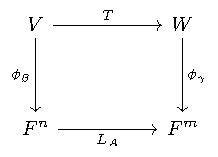
\includegraphics[width=0.55\textwidth]{figuras/diagrama-phi-beta-LA.pdf}
        \caption{Relación entre $T$ y $L_A$ vía las representaciones estándar $\phi_\BB$ y $\phi_\gamma$.}
    \end{figure}

    Sean $V$ y $W$ espacios vectoriales de dimensión $n$ y $m$, respectivamente, y sea $T:V\to W$ una transformación lineal. Definamos $A=[T]_\BB^\gamma$, donde $\BB$ y $\gamma$ son bases ordenadas arbitrarias de $V$ y $W$, respectivamente. Estamos ahora en condiciones de usar $\phi_\BB$ y $\phi_\gamma$ para estudiar la relación entre las transformaciones lineales $T$ y $L_A:F^n\to F^m$.

    Consideremos primero la Figura~2.2. Notemos que existen dos composiciones de transformaciones lineales que mandan $V$ en $F^m$:
    \begin{enumerate}
        \item Mandar $V$ a $F^n$ con $\phi_\BB$ y seguir esta transformación con $L_A$; esto produce la composición $L_A\phi_\BB$.
        \item Mandar $V$ a $W$ con $T$ y seguirla con $\phi_\gamma$ para obtener la composición $\phi_\gamma T$.
    \end{enumerate}
    Por una simple reformulación del Teorema~2.15, podemos concluir que
    \begin{equation*}
        L_A\phi_\BB=\phi_\gamma T;
    \end{equation*}
    es decir, el diagrama \textquotedblleft conmuta\textquotedblright. Heurísticamente, esta relación indica que, una vez que $V$ y $W$ se identifican con $F^n$ y $F^m$ mediante $\phi_\BB$ y $\phi_\gamma$, respectivamente, podemos \textquotedblleft identificar\textquotedblright\ a $T$ con $L_A$. Este diagrama nos permite transferir operaciones sobre espacios vectoriales abstractos a operaciones sobre $F^n$ y $F^m$.

    \begin{ejemplo}
        Recordemos la transformación lineal $T:P_3(\R)\to P_2(\R)$ definida en el Ejemplo~18 de la Sección~2.2 ($T(f(x))=f'(x)$). Sean $\BB$ y $\gamma$ las bases ordenadas estándar de $P_3(\R)$ y $P_2(\R)$, respectivamente, y sean $\phi_\BB:P_3(\R)\to\R^4$ y $\phi_\gamma:P_2(\R)\to\R^3$ las representaciones estándar correspondientes de $P_3(\R)$ y $P_2(\R)$. Si $A=[T]_\BB^\gamma$, entonces
        \begin{equation*}
            A=\begin{pmatrix}0&1&0&0\\0&0&2&0\\0&0&0&3\end{pmatrix}.
        \end{equation*}
        Consideremos el polinomio $p(x)=2+x-3x^2+5x^3$. Mostramos que $L_A\phi_\BB\big(p(x)\big)=\phi_\gamma T\big(p(x)\big)$. Ahora
        \begin{equation*}
            L_A\phi_\BB\big(p(x)\big)=\begin{pmatrix}0&1&0&0\\0&0&2&0\\0&0&0&3\end{pmatrix}\begin{pmatrix}2\\1\\-3\\5\end{pmatrix}=\begin{pmatrix}1\\-6\\15\end{pmatrix}.
        \end{equation*}
        Pero como $T\big(p(x)\big)=p'(x)=1-6x+15x^2$, tenemos
        \begin{equation*}
            \phi_\gamma T\big(p(x)\big)=\begin{pmatrix}1\\-6\\15\end{pmatrix}.
        \end{equation*}
        Así $L_A\phi_\BB\big(p(x)\big)=\phi_\gamma T\big(p(x)\big)$.
    \end{ejemplo}

    Se invita al lector a repetir este ejemplo con distintos polinomios $p(x)$.

    \begin{ejercicio}
        Etiquete las siguientes afirmaciones como verdaderas o falsas. En cada inciso, $V$ y $W$ son espacios vectoriales con bases ordenadas (finitas) $\alpha$ y $\BB$, respectivamente, $T:V\to W$ es lineal, y $A$ y $B$ son matrices.
        \begin{enumerate}[label=(\alph*)]
            \item $\big([T]_\alpha^\BB\big)^{-1}=[T^{-1}]_\BB^\alpha$.
            \item $T$ es invertible si y solo si $T$ es inyectiva y sobreyectiva.
            \item $T=L_A$, donde $A=[T]_\alpha^\BB$.
            \item $M_{2\times 3}(F)$ es isomorfo a $F^5$.
            \item $P_n(F)$ es isomorfo a $P_m(F)$ si y solo si $n=m$.
            \item $AB=I$ implica que $A$ y $B$ son invertibles.
            \item Si $A$ es invertible, entonces $(A^{-1})^{-1}=A$.
            \item $A$ es invertible si y solo si $L_A$ es invertible.
            \item $A$ debe ser cuadrada para poseer una inversa.
        \end{enumerate}
    \end{ejercicio}

    \begin{ejercicio}
        Para cada una de las siguientes transformaciones lineales $T$, determine si $T$ es invertible, y justifique su respuesta.
        \begin{enumerate}[label=(\alph*)]
            \item $T:\R^2\to\R^3$ definida por $T(a_1,a_2)=(a_1-2a_2,\,a_2,\,3a_1+4a_2)$.
            \item $T:\R^2\to\R^3$ definida por $T(a_1,a_2)=(3a_1-a_2,\,a_2,\,4a_1)$.
            \item $T:\R^3\to\R^3$ definida por $T(a_1,a_2,a_3)=(3a_1-2a_3,\,a_2,\,3a_1+4a_2)$.
            \item $T:P_3(\R)\to P_2(\R)$ definida por $T(p(x))=p'(x)$.
            \item $T:M_{2\times 2}(\R)\to P_2(\R)$ definida por
            \begin{equation*}
                T\begin{pmatrix}a&b\\c&d\end{pmatrix}=a+2bx+(c+d)x^2.
            \end{equation*}
            \item $T:M_{2\times 2}(\R)\to M_{2\times 2}(\R)$ definida por
            \begin{equation*}
                T\begin{pmatrix}a&b\\c&d\end{pmatrix}=\begin{pmatrix}a+b&a\\c&c+d\end{pmatrix}.
            \end{equation*}
        \end{enumerate}
    \end{ejercicio}

    \begin{ejercicio}
        ¿Cuáles de los siguientes pares de espacios vectoriales son isomorfos? Justifique sus respuestas.
        \begin{enumerate}[label=(\alph*)]
            \item $F^3$ y $P_3(F)$.
            \item $F^4$ y $P_3(F)$.
            \item $M_{2\times 2}(\R)$ y $P_3(\R)$.
            \item $V=\{A\in M_{2\times 2}(\R):\Tr(A)=0\}$ y $\R^4$.
        \end{enumerate}
    \end{ejercicio}

    \begin{ejercicio}
        Sean $A$ y $B$ matrices $n\times n$ invertibles. Pruebe que $AB$ es invertible y que $(AB)^{-1}=B^{-1}A^{-1}$.
    \end{ejercicio}

    \begin{ejercicio}
        Sea $A$ invertible. Pruebe que $A^t$ es invertible y que $(A^t)^{-1}=(A^{-1})^t$.
    \end{ejercicio}

    \begin{ejercicio}
        Pruebe que si $A$ es invertible y $AB=O$, entonces $B=O$.
    \end{ejercicio}

    \begin{ejercicio}
        Sea $A$ una matriz $n\times n$.
        \begin{enumerate}[label=(\alph*)]
            \item Suponga que $A^2=O$. Pruebe que $A$ no es invertible.
            \item Suponga que $AB=O$ para alguna matriz $B$ no nula $n\times n$. ¿Podría $A$ ser invertible? Explique.
        \end{enumerate}
    \end{ejercicio}

    \begin{ejercicio}
        Pruebe los Corolarios~1 y 2 del Teorema~2.19.
    \end{ejercicio}

    \begin{ejercicio}
        Sean $A$ y $B$ matrices $n\times n$ tales que $AB$ es invertible. Pruebe que $A$ y $B$ son invertibles. Dé un ejemplo para mostrar que matrices arbitrarias $A$ y $B$ no necesitan ser invertibles si $AB$ es invertible.
    \end{ejercicio}

    \begin{ejercicio}
        Sean $A$ y $B$ matrices $n\times n$ tales que $AB=I_n$.
        \begin{enumerate}[label=(\alph*)]
            \item Use el ejercicio anterior para concluir que $A$ y $B$ son invertibles.
            \item Pruebe que $A=B^{-1}$ (y por tanto $B=A^{-1}$). (Estamos, en efecto, diciendo que, para matrices cuadradas, una inversa \textquotedblleft de un solo lado\textquotedblright\ es una inversa \textquotedblleft de dos lados\textquotedblright.)
            \item Enuncie y pruebe resultados análogos para transformaciones lineales definidas sobre espacios vectoriales de dimensión finita.
        \end{enumerate}
    \end{ejercicio}

    \begin{ejercicio}
        Verifique que la transformación del Ejemplo~27 es inyectiva.
    \end{ejercicio}

    \begin{ejercicio}
        Pruebe el Teorema~2.22.
    \end{ejercicio}

    \begin{ejercicio}
        Sea $\sim$ la relación \textquotedblleft es isomorfo a\textquotedblright. Pruebe que $\sim$ es una relación de equivalencia en la clase de los espacios vectoriales sobre $F$.
    \end{ejercicio}

    \begin{ejercicio}
        Sea
        \begin{equation*}
            V=\left\{\begin{pmatrix}a&a+b\\0&c\end{pmatrix}:a,b,c\in F\right\}.
        \end{equation*}
        Construya un isomorfismo de $V$ a $F^3$.
    \end{ejercicio}

    \begin{ejercicio}
        Sean $V$ y $W$ espacios vectoriales de dimensión finita, y sea $T:V\to W$ una transformación lineal. Suponga que $\BB$ es una base para $V$. Pruebe que $T$ es un isomorfismo si y solo si $T(\BB)$ es una base para $W$.
    \end{ejercicio}

    \begin{ejercicio}
        Sea $B$ una matriz $n\times n$ invertible. Definamos $\Phi:M_{n\times n}(F)\to M_{n\times n}(F)$ por $\Phi(A)=B^{-1}AB$. Pruebe que $\Phi$ es un isomorfismo.
    \end{ejercicio}

    \begin{ejercicio}
        Sean $V$ y $W$ espacios vectoriales de dimensión finita, y sea $T:V\to W$ un isomorfismo. Sea $V_0$ un subespacio de $V$.
        \begin{enumerate}[label=(\alph*)]
            \item Pruebe que $T(V_0)$ es un subespacio de $W$.
            \item Pruebe que $\dim(V_0)=\dim\big(T(V_0)\big)$.
        \end{enumerate}
    \end{ejercicio}

    \begin{ejercicio}
        Sea $A$ una matriz $n\times n$ y sean $T:V\to W$ una transformación lineal entre un espacio vectorial $V$ de dimensión $n$ y un espacio vectorial $W$ de dimensión $m$. Sean $\BB$ y $\gamma$ bases ordenadas para $V$ y $W$, respectivamente. Pruebe que $\rg(T)=\rg(L_A)$ y $\nul(T)=\nul(L_A)$, donde $A=[T]_\BB^\gamma$. \textit{Sugerencia:} Aplique el Ejercicio~97 a la Figura~2.2.
    \end{ejercicio}

    \begin{ejercicio}
        Sean $V$ y $W$ espacios vectoriales de dimensión finita con bases ordenadas $\BB=\{v_1,v_2,\dots,v_n\}$ y $\gamma=\{w_1,w_2,\dots,w_m\}$, respectivamente. Por el Teorema~2.6, existen transformaciones lineales $T_{ij}:V\to W$ tales que
        \begin{equation*}
            T_{ij}(v_k)=\begin{cases}w_i&\text{si }k=j\\0&\text{si }k\neq j.\end{cases}
        \end{equation*}
        Primero pruebe que $\{T_{ij}:1\leq i\leq m,\,1\leq j\leq n\}$ es una base para $\mathcal{L}(V,W)$. Luego sea $M^{ij}$ la matriz $m\times n$ con un $1$ en el renglón $i$ y la columna $j$, y con $0$ en las demás entradas, y pruebe que $[T_{ij}]_\BB^\gamma=M^{ij}$. De nuevo, por el Teorema~2.6, existe una transformación lineal $\Phi:\mathcal{L}(V,W)\to M_{m\times n}(F)$ tal que $\Phi(T_{ij})=M^{ij}$. Pruebe que $\Phi$ es un isomorfismo.
    \end{ejercicio}

    \begin{ejercicio}
        Sean $c_0,c_1,\dots,c_n$ escalares distintos de un campo infinito $F$. Definamos $T:P_n(F)\to F^{n+1}$ por $T(f)=\big(f(c_0),f(c_1),\dots,f(c_n)\big)$. Pruebe que $T$ es un isomorfismo. \textit{Sugerencia:} Use los polinomios de Lagrange asociados a $c_0,c_1,\dots,c_n$.
    \end{ejercicio}

    \begin{ejercicio}
        Sea $V$ el espacio vectorial definido en el Ejemplo~7 de la Sección~1.2, y sea $W=P(F)$. Definamos
        \begin{equation*}
            T:V\to W \qquad\text{por}\qquad T(\sigma)=\sum_{i=0}^{n}\sigma(i)x^i,
        \end{equation*}
        donde $n$ es el mayor entero tal que $\sigma(n)\neq 0$. Pruebe que $T$ es un isomorfismo.
    \end{ejercicio}

    El siguiente ejercicio requiere familiaridad con el concepto de \textit{espacio cociente} definido en el Ejercicio~60 de la Sección~1.3 y con el Ejercicio~40 de la Sección~2.1.

    \begin{ejercicio}
        Sea $T:V\to Z$ una transformación lineal de un espacio vectorial $V$ sobre un espacio vectorial $Z$. Definamos la función
        \begin{equation*}
            \overline{T}:V/\ker(T)\to Z \qquad\text{por}\qquad \overline{T}\big(v+\ker(T)\big)=T(v)
        \end{equation*}
        para cualquier coseto $v+\ker(T)$ en $V/\ker(T)$.
        \begin{enumerate}[label=(\alph*)]
            \item Pruebe que $\overline{T}$ está bien definida; es decir, pruebe que si $v+\ker(T)=v'+\ker(T)$, entonces $T(v)=T(v')$.
            \item Pruebe que $\overline{T}$ es lineal.
            \item Pruebe que $\overline{T}$ es un isomorfismo.
            \item Pruebe que el diagrama mostrado en la Figura~2.3 conmuta; es decir, pruebe que $T=\overline{T}\eta$.
        \end{enumerate}
    \end{ejercicio}

    \begin{figure}[H]
        \centering
        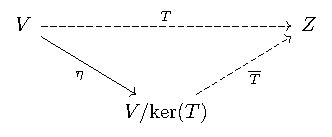
\includegraphics[width=0.5\textwidth]{figuras/diagrama-cociente-T-barra.pdf}
        \caption{El diagrama del Ejercicio~102.}
    \end{figure}

    \begin{ejercicio}
        Sea $V$ un espacio vectorial no nulo sobre un campo $F$, y supongamos que $S$ es una base para $V$. (Por el corolario al Teorema~1.14 de la Sección~1.7, todo espacio vectorial tiene una base.) Sea $\mathcal{C}(S,F)$ el espacio vectorial de todas las funciones $f\in\mathcal{F}(S,F)$ tales que $f(s)=0$ para todos, salvo un número finito, de los vectores de $S$. (Véase el Ejercicio~43 de la Sección~1.3.) Sea $\Psi:\mathcal{C}(S,F)\to V$ la función definida por
        \begin{equation*}
            \Psi(f)=\sum_{s\in S,\,f(s)\neq 0}f(s)s.
        \end{equation*}
        Pruebe que $\Psi$ es un isomorfismo. Así, todo espacio vectorial no nulo puede verse como un espacio de funciones.
    \end{ejercicio}

    \section{La matriz de cambio de coordenadas}

    En muchas áreas de las matemáticas, se usa un cambio de variable para simplificar la apariencia de una expresión. Por ejemplo, en cálculo, una antiderivada de $2xe^{x^2}$ puede encontrarse mediante el cambio de variable $u=x^2$. La expresión resultante tiene una forma tan sencilla que su antiderivada se reconoce fácilmente:
    \begin{equation*}
        \int 2xe^{x^2}\,dx=\int e^u\,du=e^u+c=e^{x^2}+c.
    \end{equation*}

    De manera similar, en geometría, el cambio de variable
    \begin{equation*}
        x=\frac{2}{\sqrt5}x'-\frac{1}{\sqrt5}y' \qquad\text{y}\qquad y=\frac{1}{\sqrt5}x'+\frac{2}{\sqrt5}y'
    \end{equation*}
    puede usarse para transformar la ecuación $2x^2-4xy+5y^2=1$ en la ecuación más simple $(x')^2+6(y')^2=1$, en cuya forma se reconoce fácilmente que se trata de la ecuación de una elipse. (Véase la Figura~2.4.) Veremos más adelante, cuando estudiemos la diagonalización de operadores autoadjuntos, cómo se determina este cambio de variable.

    \begin{figure}[H]
        \centering
        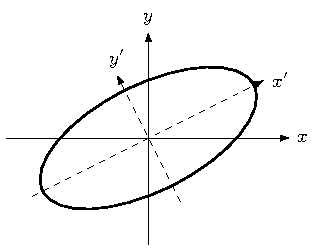
\includegraphics[width=0.45\textwidth]{figuras/elipse-cambio-coordenadas.pdf}
        \caption{Cambio de coordenadas que transforma $2x^2-4xy+5y^2=1$ en $(x')^2+6(y')^2=1$.}
    \end{figure}

    Geométricamente, el cambio de variable
    \begin{equation*}
        \begin{pmatrix}x\\y\end{pmatrix}\to\begin{pmatrix}x'\\y'\end{pmatrix}
    \end{equation*}
    es un cambio en la manera en que se describe la posición de un punto $P$ en el plano. Esto se logra introduciendo un nuevo marco de referencia, un sistema de coordenadas $x'y'$ con ejes rotados respecto a los ejes $xy$ originales. En este caso, los nuevos ejes coordenados se eligen de modo que estén en la dirección de los ejes de la elipse. Los vectores unitarios a lo largo del eje $x'$ y del eje $y'$ forman la base ordenada
    \begin{equation*}
        \BB'=\left\{\frac{1}{\sqrt5}\begin{pmatrix}2\\1\end{pmatrix},\ \frac{1}{\sqrt5}\begin{pmatrix}-1\\2\end{pmatrix}\right\}
    \end{equation*}
    para $\R^2$, y el cambio de variable es en realidad un cambio de $[P]_\BB=\begin{pmatrix}x\\y\end{pmatrix}$, el vector de coordenadas de $P$ relativo a la base ordenada estándar $\BB=\{e_1,e_2\}$, a $[P]_{\BB'}=\begin{pmatrix}x'\\y'\end{pmatrix}$, el vector de coordenadas de $P$ relativo a la nueva base rotada $\BB'$.

    Surge una pregunta natural: ¿cómo puede cambiarse un vector de coordenadas relativo a una base en un vector de coordenadas relativo a la otra? Notemos que el sistema de ecuaciones que relaciona las coordenadas nuevas y las viejas puede representarse mediante la ecuación matricial
    \begin{equation*}
        \begin{pmatrix}x\\y\end{pmatrix}=\frac{1}{\sqrt5}\begin{pmatrix}2&-1\\1&2\end{pmatrix}\begin{pmatrix}x'\\y'\end{pmatrix}.
    \end{equation*}
    Notemos también que la matriz
    \begin{equation*}
        Q=\frac{1}{\sqrt5}\begin{pmatrix}2&-1\\1&2\end{pmatrix}
    \end{equation*}
    es igual a $[I]_{\BB'}^\BB$, donde $I$ denota la transformación identidad sobre $\R^2$. Así $[v]_\BB=Q[v]_{\BB'}$ para todo $v\in\R^2$. Un resultado similar es válido en general.

    \begin{teorema}
        Sean $\BB$ y $\BB'$ dos bases ordenadas para un espacio vectorial de dimensión finita $V$, y sea $Q=[I]_{\BB'}^\BB$. Entonces:
        \begin{enumerate}[label=(\alph*)]
            \item $Q$ es invertible.
            \item Para cualquier $v\in V$, $[v]_\BB=Q[v]_{\BB'}$.
        \end{enumerate}
    \end{teorema}

    \begin{proof}
        (a) Como $I_V$ es invertible, $Q$ es invertible por el Teorema~2.18.

        (b) Para cualquier $v\in V$,
        \begin{equation*}
            [v]_\BB=[I_V(v)]_\BB=[I_V]_{\BB'}^\BB[v]_{\BB'}=Q[v]_{\BB'}
        \end{equation*}
        por el Teorema~2.14.
    \end{proof}

    A la matriz $Q=[I]_{\BB'}^\BB$ definida en el teorema anterior se le llama una \textbf{matriz de cambio de coordenadas}. Debido al inciso (b) del teorema, decimos que $Q$ \textbf{cambia $\BB'$-coordenadas en $\BB$-coordenadas}. Observemos que, si $\BB=\{x_1,x_2,\dots,x_n\}$ y $\BB'=\{x_1',x_2',\dots,x_n'\}$, entonces
    \begin{equation*}
        x_j'=\sum_{i=1}^{n}Q_{ij}x_i
    \end{equation*}
    para $j=1,2,\dots,n$; es decir, la $j$-ésima columna de $Q$ es $[x_j']_\BB$.

    Notemos que, si $Q$ cambia $\BB'$-coordenadas en $\BB$-coordenadas, entonces $Q^{-1}$ cambia $\BB$-coordenadas en $\BB'$-coordenadas. (Véase el Ejercicio~114.)

    \begin{ejemplo}
        En $\R^2$, sean $\BB=\{(1,1),(1,-1)\}$ y $\BB'=\{(2,4),(3,1)\}$. Como
        \begin{equation*}
            (2,4)=3(1,1)-1(1,-1) \qquad\text{y}\qquad (3,1)=2(1,1)+1(1,-1),
        \end{equation*}
        la matriz que cambia $\BB'$-coordenadas en $\BB$-coordenadas es
        \begin{equation*}
            Q=\begin{pmatrix}3&2\\-1&1\end{pmatrix}.
        \end{equation*}
        Así, por ejemplo,
        \begin{equation*}
            [(2,4)]_\BB=Q[(2,4)]_{\BB'}=Q\begin{pmatrix}1\\0\end{pmatrix}=\begin{pmatrix}3\\-1\end{pmatrix}.
        \end{equation*}
    \end{ejemplo}

    Para el resto de esta sección, solo consideramos transformaciones lineales que mandan un espacio vectorial $V$ en sí mismo. A una transformación lineal de este tipo se le llama un \textbf{operador lineal} sobre $V$. Supongamos ahora que $T$ es un operador lineal sobre un espacio vectorial de dimensión finita $V$, y que $\BB$ y $\BB'$ son bases ordenadas para $V$. Entonces $T$ puede representarse mediante las matrices $[T]_\BB$ y $[T]_{\BB'}$. ¿Cuál es la relación entre estas dos matrices? El siguiente teorema proporciona una respuesta sencilla, usando una matriz de cambio de coordenadas.

    \begin{teorema}
        Sea $T$ un operador lineal sobre un espacio vectorial de dimensión finita $V$, y sean $\BB$ y $\BB'$ bases ordenadas para $V$. Supongamos que $Q$ es la matriz de cambio de coordenadas que cambia $\BB'$-coordenadas en $\BB$-coordenadas. Entonces
        \begin{equation*}
            [T]_{\BB'}=Q^{-1}[T]_\BB Q.
        \end{equation*}
    \end{teorema}

    \begin{proof}
        Sea $I$ la transformación identidad sobre $V$. Entonces $T=IT=TI$; así, por el Teorema~2.11,
        \begin{equation*}
            Q[T]_{\BB'}=[I]_{\BB'}^\BB[T]_{\BB'}=[IT]_{\BB'}^\BB=[T]_{\BB'}^\BB=[TI]_{\BB'}^\BB=[T]_\BB[I]_{\BB'}^\BB=[T]_\BB Q.
        \end{equation*}
        Por tanto $[T]_{\BB'}=Q^{-1}[T]_\BB Q$.
    \end{proof}

    Una consecuencia útil del Teorema~2.23 se enuncia en el siguiente corolario.

    \begin{corolario}
        Sea $A\in M_{n\times n}(F)$, y sea $\gamma$ una base ordenada para $F^n$. Entonces $[L_A]_\gamma=Q^{-1}AQ$, donde $Q$ es la matriz $n\times n$ cuya $j$-ésima columna es el $j$-ésimo vector de $\gamma$.
    \end{corolario}

    \begin{proof}
        Sea $\BB$ la base ordenada estándar de $F^n$. Por el Teorema~2.15(a), $[L_A]_\BB=A$. Como $Q=[I]_\gamma^\BB$ tiene como $j$-ésima columna a $[x_j]_\BB=x_j$ (el $j$-ésimo vector de $\gamma$, ya que $\BB$ es la base estándar), $Q$ es la matriz de cambio de coordenadas que cambia $\gamma$-coordenadas en $\BB$-coordenadas. Por el teorema anterior (aplicado a $T=L_A$, con $\BB'=\gamma$), $[L_A]_\gamma=Q^{-1}[L_A]_\BB Q=Q^{-1}AQ$.
    \end{proof}

    \begin{ejemplo}
        Sea
        \begin{equation*}
            A=\begin{pmatrix}2&1&0\\1&1&3\\0&-1&0\end{pmatrix},
        \end{equation*}
        y sea
        \begin{equation*}
            \gamma=\left\{\begin{pmatrix}-1\\0\\0\end{pmatrix},\begin{pmatrix}2\\1\\0\end{pmatrix},\begin{pmatrix}1\\1\\1\end{pmatrix}\right\},
        \end{equation*}
        una base ordenada para $\R^3$. Sea $Q$ la matriz $3\times 3$ cuya $j$-ésima columna es el $j$-ésimo vector de $\gamma$. Entonces
        \begin{equation*}
            Q=\begin{pmatrix}-1&2&1\\0&1&1\\0&0&1\end{pmatrix} \qquad\text{y}\qquad Q^{-1}=\begin{pmatrix}-1&2&-1\\0&1&-1\\0&0&1\end{pmatrix}.
        \end{equation*}
        Así, por el corolario anterior,
        \begin{equation*}
            [L_A]_\gamma=Q^{-1}AQ=\begin{pmatrix}0&2&8\\-1&4&6\\0&-1&-1\end{pmatrix}.
        \end{equation*}
    \end{ejemplo}

    La relación entre las matrices $[T]_{\BB'}$ y $[T]_\BB$ del Teorema~2.23 será estudiada con más profundidad más adelante, cuando abordemos la diagonalización de operadores, los espacios con producto interno y las formas canónicas. Por ahora, introducimos el nombre para esta relación.

    \begin{definicion}[Matrices similares]
        Sean $A$ y $B$ matrices en $M_{n\times n}(F)$. Decimos que $B$ es \textbf{similar} a $A$ si existe una matriz invertible $Q$ tal que $B=Q^{-1}AQ$.
    \end{definicion}

    Observemos que la relación de similaridad es una relación de equivalencia (véase el Ejercicio~112). Así, basta con decir que $A$ y $B$ son similares.

    Notemos también que, en esta terminología, el Teorema~2.23 puede enunciarse como sigue: si $T$ es un operador lineal sobre un espacio vectorial de dimensión finita $V$, y si $\BB$ y $\BB'$ son bases ordenadas cualesquiera para $V$, entonces $[T]_{\BB'}$ es similar a $[T]_\BB$.

    El Teorema~2.23 puede generalizarse para permitir $T:V\to W$, donde $V$ es distinto de $W$. En este caso, podemos cambiar de base tanto en $V$ como en $W$ (véase el Ejercicio~111).

    \begin{ejemplo}
        Sea $T$ el operador lineal sobre $\R^2$ definido por
        \begin{equation*}
            T\begin{pmatrix}a\\b\end{pmatrix}=\begin{pmatrix}3a-b\\a+3b\end{pmatrix},
        \end{equation*}
        y sean $\BB$ y $\BB'$ las bases ordenadas del Ejemplo~30. El lector debe verificar que
        \begin{equation*}
            [T]_\BB=\begin{pmatrix}3&1\\-1&3\end{pmatrix}.
        \end{equation*}
        En el Ejemplo~30 vimos que la matriz de cambio de coordenadas que cambia $\BB'$-coordenadas en $\BB$-coordenadas es
        \begin{equation*}
            Q=\begin{pmatrix}3&2\\-1&1\end{pmatrix},
        \end{equation*}
        y se verifica fácilmente que
        \begin{equation*}
            Q^{-1}=\frac{1}{5}\begin{pmatrix}1&-2\\1&3\end{pmatrix}.
        \end{equation*}
        Por tanto, por el Teorema~2.23,
        \begin{equation*}
            [T]_{\BB'}=Q^{-1}[T]_\BB Q=\begin{pmatrix}4&1\\-2&2\end{pmatrix}.
        \end{equation*}
        Para mostrar que esta es la matriz correcta, podemos verificar que la imagen bajo $T$ de cada vector de $\BB'$ es la combinación lineal de los vectores de $\BB'$ con las entradas de la columna correspondiente como coeficientes. Por ejemplo, la imagen del segundo vector de $\BB'$ es
        \begin{equation*}
            T\begin{pmatrix}3\\1\end{pmatrix}=\begin{pmatrix}8\\6\end{pmatrix}=1\begin{pmatrix}2\\4\end{pmatrix}+2\begin{pmatrix}3\\1\end{pmatrix}.
        \end{equation*}
        Notemos que los coeficientes de la combinación lineal son las entradas de la segunda columna de $[T]_{\BB'}$.
    \end{ejemplo}

    A menudo es útil aplicar el Teorema~2.23 para calcular $[T]_\BB$, como muestra el siguiente ejemplo.

    \begin{ejemplo}
        Recordemos la reflexión respecto al eje $x$ del Ejemplo~3 de la Sección~2.1. La regla $(x,y)\mapsto(x,-y)$ es fácil de obtener. Derivamos ahora la regla, menos evidente, para la reflexión $T$ respecto a la recta $y=2x$. (Véase la Figura~2.5.) Deseamos encontrar una expresión para $T(a,b)$, para cualquier $(a,b)$ en $\R^2$. Como $T$ es lineal, queda completamente determinada por sus valores en una base para $\R^2$. Claramente, $T(1,2)=(1,2)$ y $T(-2,1)=-(-2,1)=(2,-1)$. Por tanto, si tomamos
        \begin{equation*}
            \BB'=\left\{\begin{pmatrix}1\\2\end{pmatrix},\begin{pmatrix}-2\\1\end{pmatrix}\right\},
        \end{equation*}
        entonces $\BB'$ es una base ordenada para $\R^2$ y
        \begin{equation*}
            [T]_{\BB'}=\begin{pmatrix}1&0\\0&-1\end{pmatrix}.
        \end{equation*}
        Sea $\BB$ la base ordenada estándar para $\R^2$, y sea $Q$ la matriz que cambia $\BB'$-coordenadas en $\BB$-coordenadas. Entonces
        \begin{equation*}
            Q=\begin{pmatrix}1&-2\\2&1\end{pmatrix}
        \end{equation*}
        y $Q^{-1}[T]_\BB Q=[T]_{\BB'}$. Podemos resolver esta ecuación para $[T]_\BB$ y obtener $[T]_\BB=Q[T]_{\BB'}Q^{-1}$. Como
        \begin{equation*}
            Q^{-1}=\frac15\begin{pmatrix}1&2\\-2&1\end{pmatrix},
        \end{equation*}
        el lector puede verificar que
        \begin{equation*}
            [T]_\BB=\frac15\begin{pmatrix}-3&4\\4&3\end{pmatrix}.
        \end{equation*}
        Como $\BB$ es la base ordenada estándar, se sigue que $T$ es la multiplicación por la izquierda por $[T]_\BB$. Así, para cualquier $(a,b)$ en $\R^2$, tenemos
        \begin{equation*}
            T\begin{pmatrix}a\\b\end{pmatrix}=\frac15\begin{pmatrix}-3&4\\4&3\end{pmatrix}\begin{pmatrix}a\\b\end{pmatrix}=\frac15\begin{pmatrix}-3a+4b\\4a+3b\end{pmatrix}.
        \end{equation*}
    \end{ejemplo}

    \begin{figure}[H]
        \centering
        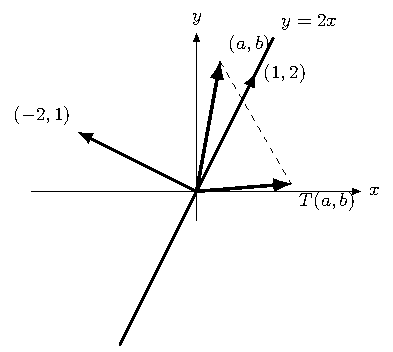
\includegraphics[width=0.6\textwidth]{figuras/reflexion-recta-y-2x.pdf}
        \caption{Reflexión respecto a la recta $y=2x$.}
    \end{figure}

    \begin{ejercicio}
        Etiquete las siguientes afirmaciones como verdaderas o falsas.
        \begin{enumerate}[label=(\alph*)]
            \item Supongamos que $\BB=\{x_1,x_2,\dots,x_n\}$ y $\BB'=\{x_1',x_2',\dots,x_n'\}$ son bases ordenadas para un espacio vectorial, y que $Q$ es la matriz de cambio de coordenadas que cambia $\BB'$-coordenadas en $\BB$-coordenadas. Entonces la $j$-ésima columna de $Q$ es $[x_j]_{\BB'}$.
            \item Toda matriz de cambio de coordenadas es invertible.
            \item Sea $T$ un operador lineal sobre un espacio vectorial de dimensión finita $V$, sean $\BB$ y $\BB'$ bases ordenadas para $V$, y sea $Q$ la matriz de cambio de coordenadas que cambia $\BB'$-coordenadas en $\BB$-coordenadas. Entonces $[T]_\BB=Q[T]_{\BB'}Q^{-1}$.
            \item Las matrices $A,B\in M_{n\times n}(F)$ se llaman similares si $B=Q^tAQ$ para alguna $Q\in M_{n\times n}(F)$.
            \item Sea $T$ un operador lineal sobre un espacio vectorial de dimensión finita $V$. Entonces, para cualesquiera bases ordenadas $\BB$ y $\gamma$ para $V$, $[T]_\BB$ es similar a $[T]_\gamma$.
        \end{enumerate}
    \end{ejercicio}

    \begin{ejercicio}
        Para cada uno de los siguientes pares de bases ordenadas $\BB$ y $\BB'$ para $\R^2$, encuentre la matriz de cambio de coordenadas que cambia $\BB'$-coordenadas en $\BB$-coordenadas.
        \begin{enumerate}[label=(\alph*)]
            \item $\BB=\{e_1,e_2\}$ y $\BB'=\{(a_1,a_2),(b_1,b_2)\}$.
            \item $\BB=\{(-1,3),(2,-1)\}$ y $\BB'=\{(0,10),(5,0)\}$.
            \item $\BB=\{(2,5),(-1,-3)\}$ y $\BB'=\{e_1,e_2\}$.
            \item $\BB=\{(-4,3),(2,-1)\}$ y $\BB'=\{(2,1),(-4,1)\}$.
        \end{enumerate}
    \end{ejercicio}

    \begin{ejercicio}
        Para cada uno de los siguientes pares de bases ordenadas $\BB$ y $\BB'$ para $P_2(\R)$, encuentre la matriz de cambio de coordenadas que cambia $\BB'$-coordenadas en $\BB$-coordenadas.
        \begin{enumerate}[label=(\alph*)]
            \item $\BB=\{x^2,x,1\}$ y $\BB'=\{a_2x^2+a_1x+a_0,\,b_2x^2+b_1x+b_0,\,c_2x^2+c_1x+c_0\}$.
            \item $\BB=\{1,x,x^2\}$ y $\BB'=\{a_2x^2+a_1x+a_0,\,b_2x^2+b_1x+b_0,\,c_2x^2+c_1x+c_0\}$.
            \item $\BB=\{2x^2-x,\,3x^2+1,\,x^2\}$ y $\BB'=\{1,x,x^2\}$.
            \item $\BB=\{x^2-x+1,\,x+1,\,x^2+1\}$ y $\BB'=\{x^2+x+4,\,4x^2-3x+2,\,2x^2+3\}$.
            \item $\BB=\{x^2-2x-3,\,-2x^2+5x+5,\,2x^2-x-3\}$ y $\BB'=\{9x-9,\,x^2+21x-2,\,3x^2+5x+2\}$.
        \end{enumerate}
    \end{ejercicio}

    \begin{ejercicio}
        Sea $T$ el operador lineal sobre $\R^2$ definido por
        \begin{equation*}
            T\begin{pmatrix}a\\b\end{pmatrix}=\begin{pmatrix}2a+b\\a-3b\end{pmatrix},
        \end{equation*}
        sea $\BB$ la base ordenada estándar para $\R^2$, y sea
        \begin{equation*}
            \BB'=\left\{\begin{pmatrix}1\\1\end{pmatrix},\begin{pmatrix}1\\2\end{pmatrix}\right\}.
        \end{equation*}
        Use el Teorema~2.23 y el hecho de que
        \begin{equation*}
            \begin{pmatrix}1&1\\1&2\end{pmatrix}^{-1}=\begin{pmatrix}2&-1\\-1&1\end{pmatrix}
        \end{equation*}
        para encontrar $[T]_{\BB'}$.
    \end{ejercicio}

    \begin{ejercicio}
        Sea $T$ el operador lineal sobre $P_1(\R)$ definido por $T(p(x))=p'(x)$, la derivada de $p(x)$. Sean $\BB=\{1,x\}$ y $\BB'=\{1+x,\,1-x\}$. Use el Teorema~2.23 y el hecho de que
        \begin{equation*}
            \begin{pmatrix}1&1\\1&-1\end{pmatrix}^{-1}=\begin{pmatrix}\tfrac12&\tfrac12\\\tfrac12&-\tfrac12\end{pmatrix}
        \end{equation*}
        para encontrar $[T]_{\BB'}$.
    \end{ejercicio}

    \begin{ejercicio}
        Para cada matriz $A$ y base ordenada $\BB$, encuentre $[L_A]_\BB$. También, encuentre una matriz invertible $Q$ tal que $[L_A]_\BB=Q^{-1}AQ$.
        \begin{enumerate}[label=(\alph*)]
            \item $A=\begin{pmatrix}1&3\\1&1\end{pmatrix}$ y $\BB=\left\{\begin{pmatrix}1\\1\end{pmatrix},\begin{pmatrix}1\\2\end{pmatrix}\right\}$.
            \item $A=\begin{pmatrix}1&2\\2&1\end{pmatrix}$ y $\BB=\left\{\begin{pmatrix}1\\1\end{pmatrix},\begin{pmatrix}1\\-1\end{pmatrix}\right\}$.
            \item $A=\begin{pmatrix}1&1&-1\\2&0&1\\1&1&0\end{pmatrix}$ y $\BB=\left\{\begin{pmatrix}1\\1\\1\end{pmatrix},\begin{pmatrix}1\\0\\1\end{pmatrix},\begin{pmatrix}1\\1\\2\end{pmatrix}\right\}$.
            \item $A=\begin{pmatrix}13&1&4\\1&13&4\\4&4&10\end{pmatrix}$ y $\BB=\left\{\begin{pmatrix}1\\1\\-2\end{pmatrix},\begin{pmatrix}1\\-1\\0\end{pmatrix},\begin{pmatrix}1\\1\\1\end{pmatrix}\right\}$.
        \end{enumerate}
    \end{ejercicio}

    \begin{ejercicio}
        En $\R^2$, sea $L$ la recta $y=mx$, con $m\neq 0$. Encuentre una expresión para $T(x,y)$, donde:
        \begin{enumerate}[label=(\alph*)]
            \item $T$ es la reflexión de $\R^2$ respecto a $L$.
            \item $T$ es la proyección sobre $L$ a lo largo de la recta perpendicular a $L$. (Véase la definición de \textit{proyección} en los ejercicios de la Sección~2.1.)
        \end{enumerate}
    \end{ejercicio}

    \begin{ejercicio}
        Pruebe la siguiente generalización del Teorema~2.23. Sea $T:V\to W$ una transformación lineal de un espacio vectorial de dimensión finita $V$ a un espacio vectorial de dimensión finita $W$. Sean $\BB$ y $\BB'$ bases ordenadas para $V$, y $\gamma$ y $\gamma'$ bases ordenadas para $W$. Entonces $[T]_{\BB'}^{\gamma'}=P^{-1}[T]_\BB^\gamma Q$, donde $Q$ es la matriz que cambia $\BB'$-coordenadas en $\BB$-coordenadas y $P$ es la matriz que cambia $\gamma'$-coordenadas en $\gamma$-coordenadas.
    \end{ejercicio}

    \begin{ejercicio}
        Pruebe que \textquotedblleft es similar a\textquotedblright\ es una relación de equivalencia en $M_{n\times n}(F)$.
    \end{ejercicio}

    \begin{ejercicio}
        Pruebe que si $A$ y $B$ son matrices similares $n\times n$, entonces $\Tr(A)=\Tr(B)$. \textit{Sugerencia:} Use el Ejercicio~70 de la Sección~2.3.
    \end{ejercicio}

    \begin{ejercicio}
        Sea $V$ un espacio vectorial de dimensión finita con bases ordenadas $\alpha$, $\BB$ y $\gamma$.
        \begin{enumerate}[label=(\alph*)]
            \item Pruebe que, si $Q$ y $R$ son las matrices de cambio de coordenadas que cambian $\alpha$-coordenadas en $\BB$-coordenadas y $\BB$-coordenadas en $\gamma$-coordenadas, respectivamente, entonces $RQ$ es la matriz de cambio de coordenadas que cambia $\alpha$-coordenadas en $\gamma$-coordenadas.
            \item Pruebe que, si $Q$ cambia $\alpha$-coordenadas en $\BB$-coordenadas, entonces $Q^{-1}$ cambia $\BB$-coordenadas en $\alpha$-coordenadas.
        \end{enumerate}
    \end{ejercicio}

    \begin{ejercicio}
        Pruebe el corolario al Teorema~2.23.
    \end{ejercicio}

    \begin{ejercicio}
        Sea $V$ un espacio vectorial de dimensión finita sobre un campo $F$, y sea $\BB=\{x_1,x_2,\dots,x_n\}$ una base ordenada para $V$. Sea $Q$ una matriz invertible $n\times n$ con entradas en $F$. Definamos
        \begin{equation*}
            x_j'=\sum_{i=1}^{n}Q_{ij}x_i \qquad\text{para }1\leq j\leq n,
        \end{equation*}
        y sea $\BB'=\{x_1',x_2',\dots,x_n'\}$. Pruebe que $\BB'$ es una base para $V$ y, por tanto, que $Q$ es la matriz de cambio de coordenadas que cambia $\BB'$-coordenadas en $\BB$-coordenadas.
    \end{ejercicio}

    \begin{ejercicio}
        Pruebe el recíproco del Ejercicio~111: si $A$ y $B$ son matrices $m\times n$ con entradas en un campo $F$, y si existen matrices invertibles $P$ (de tamaño $m\times m$) y $Q$ (de tamaño $n\times n$) tales que $B=P^{-1}AQ$, entonces existen un espacio vectorial $V$ de dimensión $n$ y un espacio vectorial $W$ de dimensión $m$ (ambos sobre $F$), bases ordenadas $\BB$ y $\BB'$ para $V$, $\gamma$ y $\gamma'$ para $W$, y una transformación lineal $T:V\to W$ tales que
        \begin{equation*}
            A=[T]_\BB^\gamma \qquad\text{y}\qquad B=[T]_{\BB'}^{\gamma'}.
        \end{equation*}
        \textit{Sugerencia:} Sean $V=F^n$, $W=F^m$, $T=L_A$, y sean $\BB$ y $\gamma$ las bases ordenadas estándar de $F^n$ y $F^m$, respectivamente. Ahora aplique los resultados del Ejercicio~116 para obtener las bases ordenadas $\BB'$ y $\gamma'$ a partir de $\BB$ y $\gamma$ vía $Q$ y $P$, respectivamente.
    \end{ejercicio}

    \section{Espacios duales}

    En esta sección nos ocupamos exclusivamente de transformaciones lineales de un espacio vectorial $V$ en su campo de escalares $F$, el cual es en sí mismo un espacio vectorial de dimensión $1$ sobre $F$. A una transformación lineal de este tipo se le llama un \textbf{funcional lineal} sobre $V$. Usualmente usamos las letras $f,g,h,\dots$ para denotar funcionales lineales. Como veremos en el Ejemplo~34, la integral definida nos proporciona uno de los ejemplos más importantes de un funcional lineal en matemáticas.

    \begin{ejemplo}
        Sea $V$ el espacio vectorial de las funciones continuas de valores reales sobre el intervalo $[0,2\pi]$. Fijemos una función $g\in V$. La función $h:V\to\R$ definida por
        \begin{equation*}
            h(x)=\frac{1}{2\pi}\int_0^{2\pi}x(t)g(t)\,dt
        \end{equation*}
        es un funcional lineal sobre $V$. En los casos en que $g(t)$ es igual a $\sin(nt)$ o $\cos(nt)$, a $h(x)$ se le suele llamar el \textbf{$n$-ésimo coeficiente de Fourier} de $x$.
    \end{ejemplo}

    \begin{ejemplo}
        Sea $V=M_{n\times n}(F)$, y definamos $f:V\to F$ por $f(A)=\Tr(A)$, la traza de $A$. Por el Ejercicio~35 de la Sección~1.3, $f$ es un funcional lineal.
    \end{ejemplo}

    \begin{ejemplo}
        Sea $V$ un espacio vectorial de dimensión finita, y sea $\BB=\{x_1,x_2,\dots,x_n\}$ una base ordenada para $V$. Para cada $i=1,2,\dots,n$, definamos $f_i(x)=a_i$, donde
        \begin{equation*}
            [x]_\BB=\begin{pmatrix}a_1\\a_2\\\vdots\\a_n\end{pmatrix}
        \end{equation*}
        es el vector de coordenadas de $x$ relativo a $\BB$. Entonces $f_i$ es un funcional lineal sobre $V$, llamado la \textbf{$i$-ésima función coordenada} respecto a la base $\BB$. Notemos que $f_i(x_j)=\delta_{ij}$, donde $\delta_{ij}$ es la delta de Kronecker. Estos funcionales lineales desempeñan un papel importante en la teoría de espacios duales (véase el Teorema~2.24).
    \end{ejemplo}

    \begin{definicion}[Espacio dual]
        Para un espacio vectorial $V$ sobre $F$, definimos el \textbf{espacio dual} de $V$ como el espacio vectorial $\mathcal{L}(V,F)$, denotado $V^*$.
    \end{definicion}

    Así $V^*$ es el espacio vectorial que consiste de todos los funcionales lineales sobre $V$, con las operaciones de suma y multiplicación por escalar definidas en la Sección~2.2. Notemos que, si $V$ es de dimensión finita, entonces, por el corolario al Teorema~2.21,
    \begin{equation*}
        \dim(V^*)=\dim\big(\mathcal{L}(V,F)\big)=\dim(V)\cdot\dim(F)=\dim(V).
    \end{equation*}
    Por tanto, por el Teorema~2.20, $V$ y $V^*$ son isomorfos. También definimos el \textbf{doble dual} $V^{**}$ de $V$ como el dual de $V^*$. En el Teorema~2.27 mostramos que, de hecho, existe una identificación natural entre $V$ y $V^{**}$ en el caso en que $V$ sea de dimensión finita.

    \begin{teorema}
        Supongamos que $V$ es un espacio vectorial de dimensión finita con base ordenada $\BB=\{x_1,x_2,\dots,x_n\}$. Sea $f_i$ ($1\leq i\leq n$) la $i$-ésima función coordenada respecto a $\BB$, definida como antes, y sea $\BB^*=\{f_1,f_2,\dots,f_n\}$. Entonces $\BB^*$ es una base ordenada para $V^*$, y, para cualquier $f\in V^*$, tenemos
        \begin{equation*}
            f=\sum_{i=1}^{n}f(x_i)f_i.
        \end{equation*}
    \end{teorema}

    \begin{proof}
        Sea $f\in V^*$. Como $\dim(V^*)=n$, basta mostrar que
        \begin{equation*}
            f=\sum_{i=1}^{n}f(x_i)f_i,
        \end{equation*}
        de lo cual se seguirá que $\BB^*$ genera a $V^*$, y por tanto es una base por el corolario~2(a) al teorema de reemplazo. Sea
        \begin{equation*}
            g=\sum_{i=1}^{n}f(x_i)f_i.
        \end{equation*}
        Para $1\leq j\leq n$, tenemos
        \begin{equation*}
            g(x_j)=\left(\sum_{i=1}^{n}f(x_i)f_i\right)(x_j)=\sum_{i=1}^{n}f(x_i)f_i(x_j)=\sum_{i=1}^{n}f(x_i)\delta_{ij}=f(x_j).
        \end{equation*}
        Por tanto $f=g$ por el corolario al Teorema~2.6.
    \end{proof}

    \begin{definicion}[Base dual]
        Usando la notación del teorema anterior, llamamos a la base ordenada $\BB^*=\{f_1,f_2,\dots,f_n\}$ de $V^*$, que satisface $f_i(x_j)=\delta_{ij}$ ($1\leq i,j\leq n$), la \textbf{base dual} de $\BB$.
    \end{definicion}

    \begin{ejemplo}
        Sea $\BB=\{(2,1),(3,1)\}$ una base ordenada para $\R^2$. Supongamos que la base dual de $\BB$ está dada por $\BB^*=\{f_1,f_2\}$. Para determinar explícitamente una fórmula para $f_1$, consideramos las ecuaciones
        \begin{align*}
            1&=f_1(2,1)=f_1(2e_1+e_2)=2f_1(e_1)+f_1(e_2)\\
            0&=f_1(3,1)=f_1(3e_1+e_2)=3f_1(e_1)+f_1(e_2).
        \end{align*}
        Resolviendo estas ecuaciones, obtenemos $f_1(e_1)=-1$ y $f_1(e_2)=3$; es decir, $f_1(x,y)=-x+3y$. De manera análoga, puede mostrarse que $f_2(x,y)=x-2y$.
    \end{ejemplo}

    Supongamos ahora que $V$ y $W$ son espacios vectoriales de dimensión finita sobre $F$ con bases ordenadas $\BB$ y $\gamma$, respectivamente. En la Sección~2.4 probamos que existe una correspondencia biunívoca entre las transformaciones lineales $T:V\to W$ y las matrices $m\times n$ (sobre $F$) mediante la correspondencia $T\leftrightarrow[T]_\BB^\gamma$. Para una matriz de la forma $A=[T]_\BB^\gamma$, surge la pregunta de si existe o no, de alguna manera natural, una transformación lineal $U$ asociada con $T$ tal que $U$ pueda representarse mediante alguna base como $A^t$. Desde luego, si $m\neq n$, sería imposible que $U$ fuera una transformación lineal de $V$ en $W$. Respondemos ahora esta pregunta aplicando lo que ya hemos aprendido sobre espacios duales.

    \begin{teorema}
        Sean $V$ y $W$ espacios vectoriales de dimensión finita sobre $F$ con bases ordenadas $\BB$ y $\gamma$, respectivamente. Para cualquier transformación lineal $T:V\to W$, la función $T^t:W^*\to V^*$ definida por $T^t(g)=gT$ para toda $g\in W^*$ es una transformación lineal con la propiedad de que $[T^t]_{\gamma^*}^{\BB^*}=\big([T]_\BB^\gamma\big)^t$.
    \end{teorema}

    \begin{proof}
        Para $g\in W^*$, es claro que $T^t(g)=gT$ es un funcional lineal sobre $V$ y por tanto está en $V^*$. Así $T^t$ manda a $W^*$ en $V^*$. Para ver que $T^t$ es lineal, sean $g,h\in W^*$ y $c\in F$. Para todo $x\in V$,
        \begin{align*}
            T^t(cg+h)(x)&=\big((cg+h)T\big)(x)=(cg+h)\big(T(x)\big)=cg\big(T(x)\big)+h\big(T(x)\big)\\
            &=c(gT)(x)+(hT)(x)=\big(cT^t(g)+T^t(h)\big)(x),
        \end{align*}
        así que $T^t(cg+h)=cT^t(g)+T^t(h)$.

        Para completar la demostración, sean $\BB=\{x_1,x_2,\dots,x_n\}$ y $\gamma=\{y_1,y_2,\dots,y_m\}$, con bases duales $\BB^*=\{f_1,f_2,\dots,f_n\}$ y $\gamma^*=\{g_1,g_2,\dots,g_m\}$, respectivamente. Por conveniencia, sea $A=[T]_\BB^\gamma$. Para encontrar la $j$-ésima columna de $[T^t]_{\gamma^*}^{\BB^*}$, comenzamos por expresar $T^t(g_j)$ como una combinación lineal de los vectores de $\BB^*$. Por el Teorema~2.24, tenemos
        \begin{equation*}
            T^t(g_j)=g_jT=\sum_{s=1}^{n}(g_jT)(x_s)f_s.
        \end{equation*}
        Así, la entrada del renglón $i$, columna $j$, de $[T^t]_{\gamma^*}^{\BB^*}$ es
        \begin{equation*}
            (g_jT)(x_i)=g_j\big(T(x_i)\big)=g_j\left(\sum_{k=1}^{m}A_{ki}y_k\right)=\sum_{k=1}^{m}A_{ki}g_j(y_k)=\sum_{k=1}^{m}A_{ki}\delta_{jk}=A_{ji}.
        \end{equation*}
        Por tanto $[T^t]_{\gamma^*}^{\BB^*}=A^t$.
    \end{proof}

    A la transformación lineal $T^t$ definida en el Teorema~2.25 se le llama la \textbf{transpuesta} de $T$. Es claro que $T^t$ es la única transformación lineal $U$ tal que $[U]_{\gamma^*}^{\BB^*}=\big([T]_\BB^\gamma\big)^t$.

    Ilustramos el Teorema~2.25 con el siguiente ejemplo.

    \begin{ejemplo}
        Sea $T:P_1(\R)\to\R^2$ definida por $T\big(p(x)\big)=\big(p(0),p(2)\big)$. Sean $\BB$ y $\gamma$ las bases ordenadas estándar para $P_1(\R)$ y $\R^2$, respectivamente. Claramente,
        \begin{equation*}
            [T]_\BB^\gamma=\begin{pmatrix}1&0\\1&2\end{pmatrix}.
        \end{equation*}
        Calculamos $[T^t]_{\gamma^*}^{\BB^*}$ directamente a partir de la definición. Sean $\BB^*=\{f_1,f_2\}$ y $\gamma^*=\{g_1,g_2\}$. Supongamos que $[T^t]_{\gamma^*}^{\BB^*}=\begin{pmatrix}a&b\\c&d\end{pmatrix}$. Entonces $T^t(g_1)=af_1+cf_2$. Así
        \begin{equation*}
            \big(T^t(g_1)\big)(1)=(af_1+cf_2)(1)=af_1(1)+cf_2(1)=a(1)+c(0)=a.
        \end{equation*}
        Pero también
        \begin{equation*}
            \big(T^t(g_1)\big)(1)=g_1\big(T(1)\big)=g_1(1,1)=1.
        \end{equation*}
        Así $a=1$. Usando cálculos análogos, obtenemos $c=0$, $b=1$, y $d=2$. Por tanto, un cálculo directo produce
        \begin{equation*}
            [T^t]_{\gamma^*}^{\BB^*}=\begin{pmatrix}1&1\\0&2\end{pmatrix}=\big([T]_\BB^\gamma\big)^t,
        \end{equation*}
        tal como predice el Teorema~2.25.
    \end{ejemplo}

    Nos ocupamos ahora de mostrar que cualquier espacio vectorial de dimensión finita $V$ puede identificarse de manera natural con su doble dual $V^{**}$. Existe, de hecho, un isomorfismo entre $V$ y $V^{**}$ que no depende de ninguna elección de bases para los dos espacios vectoriales.

    Para un vector $x\in V$, definimos $\widehat{x}:V^*\to F$ por $\widehat{x}(f)=f(x)$ para toda $f\in V^*$. Es fácil verificar que $\widehat{x}$ es un funcional lineal sobre $V^*$, así que $\widehat{x}\in V^{**}$. La correspondencia $x\mapsto\widehat{x}$ nos permite definir el isomorfismo deseado entre $V$ y $V^{**}$.

    \begin{lema}
        Sea $V$ un espacio vectorial de dimensión finita, y sea $x\in V$. Si $\widehat{x}(f)=0$ para toda $f\in V^*$, entonces $x=0$.
    \end{lema}

    \begin{proof}
        Sea $x\neq 0$. Mostramos que existe $f\in V^*$ tal que $\widehat{x}(f)\neq 0$. Elijamos una base ordenada $\BB=\{x_1,x_2,\dots,x_n\}$ para $V$ tal que $x_1=x$. Sea $\{f_1,f_2,\dots,f_n\}$ la base dual de $\BB$. Entonces $f_1(x_1)=1\neq 0$. Sea $f=f_1$.
    \end{proof}

    \begin{teorema}
        Sea $V$ un espacio vectorial de dimensión finita, y definamos $\psi:V\to V^{**}$ por $\psi(x)=\widehat{x}$. Entonces $\psi$ es un isomorfismo.
    \end{teorema}

    \begin{proof}
        (a) $\psi$ es lineal: sean $x,y\in V$ y $c\in F$. Para $f\in V^*$, tenemos
        \begin{align*}
            \psi(cx+y)(f)&=f(cx+y)=cf(x)+f(y)=c\widehat{x}(f)+\widehat{y}(f)\\
            &=\big(c\widehat{x}+\widehat{y}\big)(f).
        \end{align*}
        Por tanto
        \begin{equation*}
            \psi(cx+y)=c\widehat{x}+\widehat{y}=c\psi(x)+\psi(y).
        \end{equation*}

        (b) $\psi$ es inyectiva: supongamos que $\psi(x)$ es el funcional cero sobre $V^*$ para algún $x\in V$. Entonces $\widehat{x}(f)=0$ para toda $f\in V^*$. Por el lema anterior, concluimos que $x=0$.

        (c) $\psi$ es un isomorfismo: esto se sigue de (b) y del hecho de que $\dim(V)=\dim(V^{**})$.
    \end{proof}

    \begin{corolario}
        Sea $V$ un espacio vectorial de dimensión finita con espacio dual $V^*$. Entonces toda base ordenada para $V^*$ es la base dual de alguna base para $V$.
    \end{corolario}

    \begin{proof}
        Sea $\{f_1,f_2,\dots,f_n\}$ una base ordenada para $V^*$. Podemos combinar los Teoremas~2.24 y 2.26 para concluir que, para esta base de $V^*$, existe una base dual $\{\widehat{x}_1,\widehat{x}_2,\dots,\widehat{x}_n\}$ en $V^{**}$, es decir, $\delta_{ij}=\widehat{x}_i(f_j)=f_j(x_i)$ para todos $i$ y $j$. Así $\{f_1,f_2,\dots,f_n\}$ es la base dual de $\{x_1,x_2,\dots,x_n\}$.
    \end{proof}

    Aunque muchas de las ideas de esta sección (por ejemplo, la existencia de un espacio dual) pueden extenderse al caso en que $V$ no sea de dimensión finita, únicamente un espacio vectorial de dimensión finita es isomorfo a su doble dual vía la función $x\mapsto\widehat{x}$. De hecho, para espacios vectoriales de dimensión infinita, ningún par entre $V$, $V^*$ y $V^{**}$ es isomorfo.

    \begin{ejercicio}
        Etiquete las siguientes afirmaciones como verdaderas o falsas. Suponga que todos los espacios vectoriales son de dimensión finita.
        \begin{enumerate}[label=(\alph*)]
            \item Toda transformación lineal es un funcional lineal.
            \item Un funcional lineal definido sobre un campo puede representarse como una matriz $1\times 1$.
            \item Todo espacio vectorial es isomorfo a su espacio dual.
            \item Todo espacio vectorial es el dual de algún otro espacio vectorial.
            \item Si $T$ es un isomorfismo de $V$ sobre $V^*$ y $\BB$ es una base ordenada finita para $V$, entonces $T(\BB)=\BB^*$.
            \item Si $T$ es una transformación lineal de $V$ a $W$, entonces el dominio de $(T^t)^t$ es $V^{**}$.
            \item Si $V$ es isomorfo a $W$, entonces $V^*$ es isomorfo a $W^*$.
            \item La derivada de una función puede considerarse como un funcional lineal sobre el espacio vectorial de las funciones diferenciables.
        \end{enumerate}
    \end{ejercicio}

    \begin{ejercicio}
        Para las siguientes funciones $f$ sobre un espacio vectorial $V$, determine cuáles son funcionales lineales.
        \begin{enumerate}[label=(\alph*)]
            \item $V=P(\R)$; $f\big(p(x)\big)=2p'(0)+p''(1)$, donde $'$ denota derivación.
            \item $V=\R^2$; $f(x,y)=(2x,4y)$.
            \item $V=M_{2\times 2}(F)$; $f(A)=\Tr(A)$.
            \item $V=\R^3$; $f(x,y,z)=x^2+y^2+z^2$.
            \item $V=P(\R)$; $f\big(p(x)\big)=\int_0^1p(t)\,dt$.
            \item $V=M_{2\times 2}(F)$; $f(A)=A_{11}$.
        \end{enumerate}
    \end{ejercicio}

    \begin{ejercicio}
        Para cada uno de los siguientes espacios vectoriales $V$ y bases $\BB$, encuentre fórmulas explícitas para los vectores de la base dual $\BB^*$ de $V^*$, como en el Ejemplo~37.
        \begin{enumerate}[label=(\alph*)]
            \item $V=\R^3$; $\BB=\{(1,0,1),(1,2,1),(0,0,1)\}$.
            \item $V=P_2(\R)$; $\BB=\{1,x,x^2\}$.
        \end{enumerate}
    \end{ejercicio}

    \begin{ejercicio}
        Sea $V=\R^3$, y definamos $f_1,f_2,f_3\in V^*$ por
        \begin{equation*}
            f_1(x,y,z)=x-2y, \qquad f_2(x,y,z)=x+y+z, \qquad f_3(x,y,z)=y-3z.
        \end{equation*}
        Pruebe que $\{f_1,f_2,f_3\}$ es una base para $V^*$, y luego encuentre una base para $V$ para la cual sea la base dual.
    \end{ejercicio}

    \begin{ejercicio}
        Sea $V=P_1(\R)$, y, para $p(x)\in V$, definamos $f_1,f_2\in V^*$ por
        \begin{equation*}
            f_1\big(p(x)\big)=\int_0^1p(t)\,dt \qquad\text{y}\qquad f_2\big(p(x)\big)=\int_0^2p(t)\,dt.
        \end{equation*}
        Pruebe que $\{f_1,f_2\}$ es una base para $V^*$, y encuentre una base para $V$ para la cual sea la base dual.
    \end{ejercicio}

    \begin{ejercicio}
        Defina $f\in(\R^2)^*$ por $f(x,y)=2x+y$ y $T:\R^2\to\R^2$ por $T(x,y)=(3x+2y,x)$.
        \begin{enumerate}[label=(\alph*)]
            \item Calcule $T^t(f)$.
            \item Calcule $[T^t]_{\BB^*}$, donde $\BB$ es la base ordenada estándar para $\R^2$ y $\BB^*=\{f_1,f_2\}$ es la base dual, encontrando escalares $a,b,c$ y $d$ tales que $T^t(f_1)=af_1+cf_2$ y $T^t(f_2)=bf_1+df_2$.
            \item Calcule $[T]_\BB$ y su transpuesta, y compare sus resultados con los de (b).
        \end{enumerate}
    \end{ejercicio}

    \begin{ejercicio}
        Sean $V=P_1(\R)$ y $W=\R^2$ con bases ordenadas estándar $\BB$ y $\gamma$, respectivamente. Definamos $T:V\to W$ por
        \begin{equation*}
            T\big(p(x)\big)=\big(p(0)-2p(1),\,p(0)+p'(0)\big),
        \end{equation*}
        donde $p'(x)$ es la derivada de $p(x)$.
        \begin{enumerate}[label=(\alph*)]
            \item Para $f\in W^*$ definida por $f(a,b)=a-2b$, calcule $T^t(f)$.
            \item Calcule $[T^t]_{\gamma^*}^{\BB^*}$, sin apelar al Teorema~2.25.
            \item Calcule $[T]_\BB^\gamma$ y su transpuesta, y compare sus resultados con los de (b).
        \end{enumerate}
    \end{ejercicio}

    \begin{ejercicio}
        Muestre que todo plano que pasa por el origen en $\R^3$ puede identificarse con el espacio nulo de un vector en $(\R^3)^*$. Enuncie un resultado análogo para $\R^2$.
    \end{ejercicio}

    \begin{ejercicio}
        Pruebe que una función $T:F^n\to F^m$ es lineal si y solo si existen funcionales lineales $f_1,f_2,\dots,f_m\in(F^n)^*$ tales que $T(x)=\big(f_1(x),f_2(x),\dots,f_m(x)\big)$ para todo $x\in F^n$. \textit{Sugerencia:} Si $T$ es lineal, defina $f_i(x)=(g_iT)(x)$ para $x\in F^n$; es decir, $f_i=T^t(g_i)$ para $1\leq i\leq m$, donde $\{g_1,g_2,\dots,g_m\}$ es la base dual de la base ordenada estándar para $F^m$.
    \end{ejercicio}

    \begin{ejercicio}
        Sean $c_0,c_1,\dots,c_n$ escalares distintos en $F$.
        \begin{enumerate}[label=(\alph*)]
            \item Para $0\leq i\leq n$, defina $f_i\in\big(P_n(F)\big)^*$ por $f_i\big(p(x)\big)=p(c_i)$. Pruebe que $\{f_0,f_1,\dots,f_n\}$ es una base para $\big(P_n(F)\big)^*$. \textit{Sugerencia:} Aplique cualquier combinación lineal de este conjunto que sea igual a la transformación cero a $p(x)=(x-c_1)(x-c_2)\cdots(x-c_n)$, y deduzca que el primer coeficiente es cero.
            \item Use el corolario al Teorema~2.26 y (a) para mostrar que existen polinomios únicos $p_0(x),p_1(x),\dots,p_n(x)$ tales que $p_i(c_j)=\delta_{ij}$ para $0\leq i\leq n$. Estos polinomios son los polinomios de Lagrange definidos en la Sección~1.6.
            \item Para cualesquiera escalares $a_0,a_1,\dots,a_n$ (no necesariamente distintos), deduzca que existe un único polinomio $q(x)$ de grado a lo más $n$ tal que $q(c_i)=a_i$ para $0\leq i\leq n$. De hecho,
            \begin{equation*}
                q(x)=\sum_{i=0}^{n}a_ip_i(x).
            \end{equation*}
            \item Deduzca la fórmula de interpolación de Lagrange:
            \begin{equation*}
                p(x)=\sum_{i=0}^{n}p(c_i)p_i(x)
            \end{equation*}
            para cualquier $p(x)\in V$.
            \item Pruebe que
            \begin{equation*}
                \int_a^bp(t)\,dt=\sum_{i=0}^{n}p(c_i)d_i,
            \end{equation*}
            donde
            \begin{equation*}
                d_i=\int_a^bp_i(t)\,dt.
            \end{equation*}
        \end{enumerate}
        Suponga ahora que
        \begin{equation*}
            c_i=a+\frac{i(b-a)}{n} \qquad\text{para }i=0,1,\dots,n.
        \end{equation*}
        Para $n=1$, el resultado anterior produce la regla del trapecio para evaluar la integral definida de un polinomio. Para $n=2$, este resultado produce la regla de Simpson para evaluar la integral definida de un polinomio.
    \end{ejercicio}

    \begin{ejercicio}
        Sean $V$ y $W$ espacios vectoriales de dimensión finita sobre $F$, y sean $\psi_1$ y $\psi_2$ los isomorfismos entre $V$ y $V^{**}$, y entre $W$ y $W^{**}$, respectivamente, definidos como en el Teorema~2.26. Sea $T:V\to W$ lineal, y defina $T^{tt}=(T^t)^t$. Pruebe que el diagrama representado en la Figura~2.6 conmuta (es decir, pruebe que $\psi_2T=T^{tt}\psi_1$).
    \end{ejercicio}

    \begin{figure}[H]
        \centering
        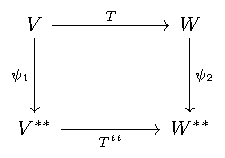
\includegraphics[width=0.5\textwidth]{figuras/diagrama-doble-dual.pdf}
        \caption{El diagrama del Ejercicio~128.}
    \end{figure}

    \begin{ejercicio}
        Sea $V$ un espacio vectorial de dimensión finita con base ordenada $\BB$. Pruebe que $\psi(\BB)=\BB^{**}$, donde $\psi$ es la función definida en el Teorema~2.26.
    \end{ejercicio}

    En los Ejercicios~13 a 17, $V$ denota un espacio vectorial de dimensión finita sobre $F$. Para cualquier subconjunto $S$ de $V$, se define el \textbf{aniquilador} $S^0$ de $S$ como
    \begin{equation*}
        S^0=\{f\in V^*:f(x)=0\text{ para todo }x\in S\}.
    \end{equation*}

    \begin{ejercicio}
        \begin{enumerate}[label=(\alph*)]
            \item Pruebe que $S^0$ es un subespacio de $V^*$.
            \item Si $W$ es un subespacio de $V$ y $x\notin W$, pruebe que existe $f\in W^0$ tal que $f(x)\neq 0$.
            \item Pruebe que $(S^0)^0=\gen{\psi(S)}$, donde $\psi$ se define como en el Teorema~2.26.
            \item Para subespacios $W_1$ y $W_2$, pruebe que $W_1=W_2$ si y solo si $W_1^0=W_2^0$.
            \item Para subespacios $W_1$ y $W_2$, muestre que $(W_1+W_2)^0=W_1^0\cap W_2^0$.
        \end{enumerate}
    \end{ejercicio}

    \begin{ejercicio}
        Pruebe que, si $W$ es un subespacio de $V$, entonces $\dim(W)+\dim(W^0)=\dim(V)$. \textit{Sugerencia:} Extienda una base ordenada $\{x_1,x_2,\dots,x_k\}$ de $W$ a una base ordenada $\BB=\{x_1,x_2,\dots,x_n\}$ de $V$. Sea $\BB^*=\{f_1,f_2,\dots,f_n\}$. Pruebe que $\{f_{k+1},f_{k+2},\dots,f_n\}$ es una base para $W^0$.
    \end{ejercicio}

    \begin{ejercicio}
        Supongamos que $W$ es un espacio vectorial de dimensión finita y que $T:V\to W$ es lineal. Pruebe que $\ker(T^t)=\big(\Im(T)\big)^0$.
    \end{ejercicio}

    \begin{ejercicio}
        Use los Ejercicios~14 y 15 para deducir que $\rg(L_{A^t})=\rg(L_A)$ para cualquier $A\in M_{m\times n}(F)$.
    \end{ejercicio}

    \begin{ejercicio}
        Sea $T$ un operador lineal sobre $V$, y sea $W$ un subespacio de $V$. Pruebe que $W$ es $T$-invariante (según se definió en los ejercicios de la Sección~2.1) si y solo si $W^0$ es $T^t$-invariante.
    \end{ejercicio}

    \begin{ejercicio}
        Sea $V$ un espacio vectorial no nulo sobre un campo $F$, y sea $S$ una base para $V$. (Por el corolario al Teorema~1.14 de la Sección~1.7, todo espacio vectorial tiene una base.) Sea $\Phi:V^*\to\mathcal{L}(S,F)$ la función definida por $\Phi(f)=f_S$, la restricción de $f$ a $S$. Pruebe que $\Phi$ es un isomorfismo. \textit{Sugerencia:} Aplique el Ejercicio~34 de la Sección~2.1.
    \end{ejercicio}

    \begin{ejercicio}
        Sea $V$ un espacio vectorial no nulo, y sea $W$ un subespacio propio de $V$ (es decir, $W\neq V$). Pruebe que existe un funcional lineal no nulo $f\in V^*$ tal que $f(x)=0$ para todo $x\in W$. \textit{Sugerencia:} Para el caso de dimensión infinita, use el Ejercicio~34 de la Sección~2.1, así como resultados sobre la extensión de conjuntos linealmente independientes a bases de la Sección~1.7.
    \end{ejercicio}

    \begin{ejercicio}
        Sean $V$ y $W$ espacios vectoriales no nulos sobre el mismo campo, y sea $T:V\to W$ una transformación lineal.
        \begin{enumerate}[label=(\alph*)]
            \item Pruebe que $T$ es sobreyectiva si y solo si $T^t$ es inyectiva.
            \item Pruebe que $T^t$ es sobreyectiva si y solo si $T$ es inyectiva.
        \end{enumerate}
        \textit{Sugerencia:} Partes de la demostración requieren el resultado del Ejercicio~136 para el caso de dimensión infinita.
    \end{ejercicio}

    \section{Ecuaciones diferenciales lineales homogéneas con coeficientes constantes}

    Como introducción a esta sección, consideremos el siguiente problema físico. Un peso de masa $m$ está sujeto a un resorte suspendido verticalmente que puede estirarse hasta que las fuerzas que actúan sobre el peso estén en equilibrio. Supongamos que el peso está ahora en reposo, e impongamos un sistema de coordenadas $xy$ con el peso en el origen y el resorte a lo largo del eje $y$ positivo (véase la Figura~2.7).

    \begin{figure}[H]
        \centering
        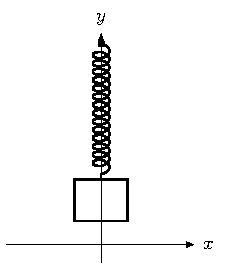
\includegraphics[width=0.3\textwidth]{figuras/resorte-peso.pdf}
        \caption{Resorte con un peso suspendido, en la posición de equilibrio.}
    \end{figure}

    Supongamos que, en cierto instante, digamos $t=0$, el peso se baja una distancia $s$ a lo largo del eje $y$ y se suelta. El resorte comienza entonces a oscilar.

    Describimos el movimiento del resorte. En cualquier instante $t\geq 0$, sea $F(t)$ la fuerza que actúa sobre el peso, y sea $y(t)$ la posición del peso a lo largo del eje $y$. Por ejemplo, $y(0)=-s$. La segunda derivada de $y$ respecto al tiempo, $y''(t)$, es la aceleración del peso en el instante $t$; por tanto, por la segunda ley de Newton,
    \begin{equation*}
        F(t)=my''(t).
    \end{equation*}
    Es razonable suponer que la fuerza que actúa sobre el peso se debe totalmente a la tensión del resorte, y que esta fuerza satisface la ley de Hooke: \textit{la fuerza que actúa sobre el peso es proporcional a su desplazamiento respecto a la posición de equilibrio, pero actúa en dirección opuesta}. Si $k>0$ es la constante de proporcionalidad, entonces la ley de Hooke establece que
    \begin{equation*}
        F(t)=-ky(t).
    \end{equation*}
    Combinando ambas ecuaciones, obtenemos $my''=-ky$, o
    \begin{equation*}
        y''+\frac{k}{m}y=0.
    \end{equation*}

    Esta expresión es un ejemplo de una \textit{ecuación diferencial}. Una \textbf{ecuación diferencial} en una función incógnita $y=y(t)$ es una ecuación que involucra a $y$, a $t$, y a derivadas de $y$. Si la ecuación diferencial tiene la forma
    \begin{equation*}
        a_ny^{(n)}+a_{n-1}y^{(n-1)}+\cdots+a_1y^{(1)}+a_0y=f, \tag{4}
    \end{equation*}
    donde $a_0,a_1,\dots,a_n$ y $f$ son funciones de $t$ y $y^{(k)}$ denota la $k$-ésima derivada de $y$, entonces se dice que la ecuación es \textbf{lineal}. A las funciones $a_i$ se les llama los \textbf{coeficientes} de la ecuación diferencial (4). Así, la ecuación $y''+(k/m)y=0$ es un ejemplo de una ecuación diferencial lineal en la que los coeficientes son constantes y la función $f$ es idénticamente cero. Cuando $f$ es idénticamente cero, a (4) se le llama \textbf{homogénea}.

    En esta sección aplicamos el álgebra lineal que hemos estudiado para resolver ecuaciones diferenciales lineales homogéneas con coeficientes constantes. Si $a_n\neq 0$, decimos que la ecuación diferencial (4) es de \textbf{orden $n$}. En este caso, dividimos ambos lados entre $a_n$ para obtener una nueva ecuación, equivalente, de la forma
    \begin{equation*}
        y^{(n)}+b_{n-1}y^{(n-1)}+\cdots+b_1y^{(1)}+b_0y=0,
    \end{equation*}
    donde $b_i=a_i/a_n$ para $i=0,1,\dots,n-1$. Debido a esta observación, siempre suponemos que el coeficiente $a_n$ en (4) es igual a $1$.

    Una \textbf{solución} de (4) es una función que, al sustituirse en lugar de $y$, reduce (4) a una identidad.

    \begin{ejemplo}
        La función $y(t)=\sin\sqrt{k/m}\,t$ es una solución de la ecuación $y''+(k/m)y=0$, pues
        \begin{equation*}
            y''(t)+\frac{k}{m}y(t)=-\frac{k}{m}\sin\sqrt{\frac{k}{m}}\,t+\frac{k}{m}\sin\sqrt{\frac{k}{m}}\,t=0
        \end{equation*}
        para todo $t$. Notemos, sin embargo, que al sustituir $y(t)=t$ en esta ecuación se obtiene
        \begin{equation*}
            y''(t)+\frac{k}{m}y(t)=\frac{k}{m}t,
        \end{equation*}
        que no es idénticamente cero. Así $y(t)=t$ no es una solución de esta ecuación.
    \end{ejemplo}

    En nuestro estudio de las ecuaciones diferenciales, resulta útil considerar las soluciones como funciones de valores complejos de una variable real, aunque las soluciones que tienen sentido físico para nosotros sean de valores reales. La conveniencia de este punto de vista se hará más clara después. Así, nos ocupamos del espacio vectorial $\mathcal{F}(\R,\C)$ (definido en el Ejemplo~5 de la Sección~1.2). Para poder considerar funciones de valores complejos de una variable real como soluciones a ecuaciones diferenciales, debemos definir qué significa derivar tales funciones. Dada una función de valores complejos $x\in\mathcal{F}(\R,\C)$ de una variable real $t$, existen funciones únicas de valores reales $x_1$ y $x_2$ de $t$ tales que
    \begin{equation*}
        x(t)=x_1(t)+ix_2(t) \qquad\text{para }t\in\R,
    \end{equation*}
    donde $i$ es el número imaginario tal que $i^2=-1$. Llamamos a $x_1$ la \textbf{parte real} y a $x_2$ la \textbf{parte imaginaria} de $x$.

    \begin{definicion}[Derivada de una función de valores complejos]
        Dada una función $x\in\mathcal{F}(\R,\C)$ con parte real $x_1$ y parte imaginaria $x_2$, decimos que $x$ es \textbf{derivable} si $x_1$ y $x_2$ son derivables. Si $x$ es derivable, definimos la \textbf{derivada} $x'$ de $x$ por
        \begin{equation*}
            x'=x_1'+ix_2'.
        \end{equation*}
    \end{definicion}

    Ilustramos algunos cálculos con funciones de valores complejos en el siguiente ejemplo.

    \begin{ejemplo}
        Supongamos que $x(t)=\cos 2t+i\sin 2t$. Entonces
        \begin{equation*}
            x'(t)=-2\sin 2t+2i\cos 2t.
        \end{equation*}
        Encontramos a continuación las partes real e imaginaria de $x^2$. Como
        \begin{align*}
            x^2(t)&=(\cos 2t+i\sin 2t)^2=(\cos^2 2t-\sin^2 2t)+i(2\sin 2t\cos 2t)\\
            &=\cos 4t+i\sin 4t,
        \end{align*}
        la parte real de $x^2(t)$ es $\cos 4t$, y la parte imaginaria es $\sin 4t$.
    \end{ejemplo}

    El siguiente teorema indica que podemos limitar nuestras investigaciones a un espacio vectorial considerablemente más pequeño que $\mathcal{F}(\R,\C)$.

    \begin{teorema}
        Toda solución a una ecuación diferencial lineal homogénea con coeficientes constantes tiene derivadas de todos los órdenes; es decir, si $x$ es una solución de tal ecuación, entonces $x^{(k)}$ existe para todo entero positivo $k$.
    \end{teorema}

    \begin{proof}
        Sea $x$ una solución de la ecuación de orden $n$
        \begin{equation*}
            y^{(n)}+a_{n-1}y^{(n-1)}+\cdots+a_1y^{(1)}+a_0y=0.
        \end{equation*}
        Por definición de solución, $x,x^{(1)},\dots,x^{(n)}$ existen, y
        \begin{equation*}
            x^{(n)}=-\big(a_{n-1}x^{(n-1)}+\cdots+a_1x^{(1)}+a_0x\big). \tag{$*$}
        \end{equation*}
        Mostramos, por inducción sobre $k\geq n$, que $x^{(k)}$ existe. El caso $k=n$ es inmediato de la definición de solución. Supongamos que $x^{(k)}$ existe para algún $k\geq n$. El lado derecho de $(*)$ es una combinación lineal, con coeficientes constantes, de $x,x^{(1)},\dots,x^{(n-1)}$, cada una de las cuales, por hipótesis de inducción, tiene al menos $k-n+1$ derivadas (pues $k\geq n$ implica $k-(n-1)\geq 1$, y de hecho, por la hipótesis de inducción aplicada repetidamente, cada una de $x,\dots,x^{(n-1)}$ tiene tantas derivadas como se necesiten hasta orden $k$). Derivando $(*)$ $(k-n+1)$ veces término a término (lo cual es válido, pues cada término $a_jx^{(j)}$, con $a_j$ constante, se deriva como $a_jx^{(j+1)}$, y estas derivadas existen por hipótesis de inducción hasta el orden requerido), concluimos que $x^{(k+1)}$ existe. Esto completa la inducción.
    \end{proof}

    \begin{ejemplo}
        Para ilustrar el teorema anterior, consideremos la ecuación
        \begin{equation*}
            y^{(2)}+4y=0.
        \end{equation*}
        Para calificar como solución, una función $y$ debe tener dos derivadas. Si $y$ es una solución, sin embargo, entonces
        \begin{equation*}
            y^{(2)}=-4y.
        \end{equation*}
        Así, como $y^{(2)}$ es un múltiplo constante de una función $y$ que tiene dos derivadas, $y^{(2)}$ debe tener dos derivadas. Por tanto $y^{(4)}$ existe; de hecho,
        \begin{equation*}
            y^{(4)}=-4y^{(2)}.
        \end{equation*}
        Como $y^{(4)}$ es un múltiplo constante de una función que hemos mostrado tiene al menos dos derivadas, también tiene al menos dos derivadas; así $y^{(6)}$ existe. Continuando de esta manera, podemos mostrar que cualquier solución tiene derivadas de todos los órdenes.
    \end{ejemplo}

    \begin{definicion}[$C^\infty$]
        Usamos $C^\infty$ para denotar el conjunto de todas las funciones en $\mathcal{F}(\R,\C)$ que tienen derivadas de todos los órdenes.
    \end{definicion}

    Es un ejercicio sencillo mostrar que $C^\infty$ es un subespacio de $\mathcal{F}(\R,\C)$ y, por tanto, un espacio vectorial sobre $\C$. En vista del teorema anterior, es este espacio vectorial el que nos interesa. Para $x\in C^\infty$, la derivada $x'$ de $x$ también está en $C^\infty$. Podemos usar la operación de derivación para definir una función $D:C^\infty\to C^\infty$ por
    \begin{equation*}
        D(x)=x' \qquad\text{para }x\in C^\infty.
    \end{equation*}
    Es fácil mostrar que $D$ es un operador lineal. Más generalmente, consideremos cualquier polinomio $p$ sobre $\C$ de la forma
    \begin{equation*}
        p(t)=a_nt^n+a_{n-1}t^{n-1}+\cdots+a_1t+a_0.
    \end{equation*}
    Si definimos
    \begin{equation*}
        p(D)=a_nD^n+a_{n-1}D^{n-1}+\cdots+a_1D+a_0I,
    \end{equation*}
    entonces $p(D)$ es un operador lineal sobre $C^\infty$.

    \begin{definicion}[Operador diferencial]
        Para cualquier polinomio $p(t)$ sobre $\C$ de grado positivo, a $p(D)$ se le llama un \textbf{operador diferencial}. El \textbf{orden} del operador diferencial $p(D)$ es el grado del polinomio $p(t)$.
    \end{definicion}

    Los operadores diferenciales son útiles porque nos brindan un medio para reformular una ecuación diferencial en el contexto del álgebra lineal. Cualquier ecuación diferencial lineal homogénea con coeficientes constantes,
    \begin{equation*}
        y^{(n)}+a_{n-1}y^{(n-1)}+\cdots+a_1y^{(1)}+a_0y=0,
    \end{equation*}
    puede reescribirse usando operadores diferenciales como
    \begin{equation*}
        \big(D^n+a_{n-1}D^{n-1}+\cdots+a_1D+a_0I\big)(y)=0.
    \end{equation*}

    \begin{definicion}[Polinomio auxiliar]
        Dada la ecuación diferencial anterior, al polinomio complejo
        \begin{equation*}
            p(t)=t^n+a_{n-1}t^{n-1}+\cdots+a_1t+a_0
        \end{equation*}
        se le llama el \textbf{polinomio auxiliar} asociado a la ecuación.
    \end{definicion}

    Por ejemplo, la ecuación del resorte tiene como polinomio auxiliar
    \begin{equation*}
        p(t)=t^2+\frac{k}{m}.
    \end{equation*}

    Cualquier ecuación diferencial lineal homogénea con coeficientes constantes puede reescribirse como
    \begin{equation*}
        p(D)(y)=0,
    \end{equation*}
    donde $p(t)$ es el polinomio auxiliar asociado a la ecuación. Claramente, esta ecuación implica el siguiente teorema.

    \begin{teorema}
        El conjunto de todas las soluciones a una ecuación diferencial lineal homogénea con coeficientes constantes coincide con el espacio nulo de $p(D)$, donde $p(t)$ es el polinomio auxiliar asociado a la ecuación.
    \end{teorema}

    \begin{proof}
        Sea la ecuación $y^{(n)}+a_{n-1}y^{(n-1)}+\cdots+a_1y^{(1)}+a_0y=0$, con polinomio auxiliar $p(t)=t^n+a_{n-1}t^{n-1}+\cdots+a_1t+a_0$. Una función $y\in C^\infty$ es solución de la ecuación si y solo si $y^{(n)}+a_{n-1}y^{(n-1)}+\cdots+a_0y=0$; pero, por definición, el lado izquierdo de esta igualdad es precisamente $p(D)(y)$. Así $y$ es solución si y solo si $p(D)(y)=0$, es decir, si y solo si $y\in\ker\big(p(D)\big)$.
    \end{proof}

    \begin{corolario}
        El conjunto de soluciones de una ecuación diferencial lineal homogénea con coeficientes constantes es un subespacio de $C^\infty$.
    \end{corolario}

    \begin{proof}
        Por el teorema anterior, este conjunto es el espacio nulo de un operador lineal, y por tanto es un subespacio de $C^\infty$ por el Teorema~2.1.
    \end{proof}

    En vista del corolario anterior, llamamos al conjunto de soluciones de una ecuación diferencial lineal homogénea con coeficientes constantes el \textbf{espacio solución} de la ecuación. Una manera práctica de describir tal espacio es en términos de una base. Examinamos ahora una cierta clase de funciones que resulta útil para encontrar bases para estos espacios solución.

    Para un número real $s$, estamos familiarizados con el número real $e^s$, donde $e$ es el único número cuyo logaritmo natural es $1$ (es decir, $\ln e=1$). Sabemos, por ejemplo, ciertas propiedades de la exponenciación, a saber,
    \begin{equation*}
        e^{s+t}=e^se^t \qquad\text{y}\qquad e^{-t}=\frac{1}{e^t}
    \end{equation*}
    para cualesquiera números reales $s$ y $t$. Extendemos ahora la definición de potencias de $e$ para incluir números complejos, de manera que estas propiedades se preserven.

    \begin{definicion}[Exponencial compleja, fórmula de Euler]
        Sea $c=a+ib$ un número complejo con parte real $a$ y parte imaginaria $b$. Definimos
        \begin{equation*}
            e^c=e^a(\cos b+i\sin b).
        \end{equation*}
        Al caso particular
        \begin{equation*}
            e^{ib}=\cos b+i\sin b
        \end{equation*}
        se le llama la \textbf{fórmula de Euler}.
    \end{definicion}

    Por ejemplo, para $c=2+i(\pi/3)$,
    \begin{equation*}
        e^c=e^2\left(\cos\frac{\pi}{3}+i\sin\frac{\pi}{3}\right)=e^2\left(\frac12+i\frac{\sqrt3}{2}\right).
    \end{equation*}
    Claramente, si $c$ es real ($b=0$), obtenemos el resultado usual: $e^c=e^a$.

    \begin{proposicion}
        Para cualesquiera números complejos $c=a+ib$ y $d=a'+ib'$, se cumplen las identidades $e^{c+d}=e^ce^d$ y $e^{-c}=1/e^c$.
    \end{proposicion}

    \begin{proof}
        Como $c+d=(a+a')+i(b+b')$, tenemos, por definición,
        \begin{equation*}
            e^{c+d}=e^{a+a'}\big(\cos(b+b')+i\sin(b+b')\big).
        \end{equation*}
        Usando que $e^{a+a'}=e^ae^{a'}$ (válido para exponentes reales) y las identidades trigonométricas de suma de ángulos $\cos(b+b')=\cos b\cos b'-\sin b\sin b'$ y $\sin(b+b')=\sin b\cos b'+\cos b\sin b'$, obtenemos
        \begin{align*}
            e^{c+d}&=e^ae^{a'}\big[(\cos b\cos b'-\sin b\sin b')+i(\sin b\cos b'+\cos b\sin b')\big]\\
            &=e^ae^{a'}\big[(\cos b+i\sin b)(\cos b'+i\sin b')\big]\\
            &=\big[e^a(\cos b+i\sin b)\big]\big[e^{a'}(\cos b'+i\sin b')\big]=e^ce^d,
        \end{align*}
        donde la penúltima igualdad se verifica expandiendo el producto $(\cos b+i\sin b)(\cos b'+i\sin b')$ y usando $i^2=-1$. Para la segunda identidad, tomando $d=-c=-a-ib$ en la primera identidad, obtenemos $e^ce^{-c}=e^{c-c}=e^0=1$, y como $e^c\neq 0$ (pues $|e^c|=e^a>0$), se sigue que $e^{-c}=1/e^c$.
    \end{proof}

    \begin{definicion}[Función exponencial]
        A una función $f:\R\to\C$ definida por $f(t)=e^{ct}$ para un número complejo fijo $c$ se le llama una \textbf{función exponencial}.
    \end{definicion}

    La derivada de una función exponencial, según se describe en el siguiente teorema, es consistente con la versión real.

    \begin{teorema}
        Para cualquier función exponencial $f(t)=e^{ct}$, $f'(t)=ce^{ct}$.
    \end{teorema}

    \begin{proof}
        Escribamos $c=a+ib$. Entonces $f(t)=e^{ct}=e^{at}(\cos bt+i\sin bt)$, así que la parte real de $f$ es $f_1(t)=e^{at}\cos bt$ y la parte imaginaria es $f_2(t)=e^{at}\sin bt$. Usando la regla del producto y la regla de la cadena (válidas para estas funciones reales de variable real),
        \begin{align*}
            f_1'(t)&=ae^{at}\cos bt-be^{at}\sin bt,\\
            f_2'(t)&=ae^{at}\sin bt+be^{at}\cos bt.
        \end{align*}
        Por tanto
        \begin{align*}
            f'(t)&=f_1'(t)+if_2'(t)=e^{at}\big[(a\cos bt-b\sin bt)+i(a\sin bt+b\cos bt)\big]\\
            &=e^{at}\big[a(\cos bt+i\sin bt)+ib(\cos bt+i\sin bt)\big]\\
            &=e^{at}(a+ib)(\cos bt+i\sin bt)=ce^{at}(\cos bt+i\sin bt)=ce^{ct}.
        \end{align*}
    \end{proof}

    Podemos usar funciones exponenciales para describir todas las soluciones a una ecuación diferencial lineal homogénea de orden $1$. Recordemos que el \textbf{orden} de tal ecuación es el grado de su polinomio auxiliar. Así una ecuación de orden $1$ es de la forma
    \begin{equation*}
        y'+a_0y=0. \tag{5}
    \end{equation*}

    \begin{teorema}
        El espacio solución de (5) tiene dimensión $1$ y tiene a $\{e^{-a_0t}\}$ como base.
    \end{teorema}

    \begin{proof}
        Claramente (5) tiene a $e^{-a_0t}$ como solución. Supongamos que $x(t)$ es cualquier solución de (5). Entonces
        \begin{equation*}
            x'(t)=-a_0x(t) \qquad\text{para todo }t\in\R.
        \end{equation*}
        Definamos
        \begin{equation*}
            z(t)=e^{a_0t}x(t).
        \end{equation*}
        Derivando $z$, obtenemos
        \begin{equation*}
            z'(t)=(e^{a_0t})'x(t)+e^{a_0t}x'(t)=a_0e^{a_0t}x(t)-a_0e^{a_0t}x(t)=0.
        \end{equation*}
        (Notemos que la regla del producto, familiar para la derivación, es válida también para funciones de valores complejos de una variable real. Una justificación de esto involucra un cálculo directo, aunque extenso, aplicando las reglas de derivación a las partes real e imaginaria de $z=e^{a_0t}x$.) Como $z'$ es idénticamente cero, $z$ es una función constante. (De nuevo, este hecho, bien conocido para funciones de valores reales, también es cierto para funciones de valores complejos; la prueba se apoya en el caso real, examinando por separado las partes real e imaginaria de $z$.) Así existe un número complejo $k$ tal que
        \begin{equation*}
            z(t)=e^{a_0t}x(t)=k \qquad\text{para todo }t\in\R.
        \end{equation*}
        Así
        \begin{equation*}
            x(t)=ke^{-a_0t}.
        \end{equation*}
        Concluimos que toda solución de (5) es una combinación lineal de $e^{-a_0t}$.
    \end{proof}

    Otra manera de enunciar el teorema anterior es la siguiente.

    \begin{corolario}
        Para cualquier número complejo $c$, el espacio nulo del operador diferencial $D-cI$ tiene a $\{e^{ct}\}$ como base.
    \end{corolario}

    Nos ocupamos ahora de las ecuaciones diferenciales de orden mayor que uno. Dada una ecuación diferencial lineal homogénea de orden $n$ con coeficientes constantes,
    \begin{equation*}
        y^{(n)}+a_{n-1}y^{(n-1)}+\cdots+a_1y^{(1)}+a_0y=0,
    \end{equation*}
    su polinomio auxiliar
    \begin{equation*}
        p(t)=t^n+a_{n-1}t^{n-1}+\cdots+a_1t+a_0
    \end{equation*}
    se factoriza en un producto de polinomios de grado $1$, es decir,
    \begin{equation*}
        p(t)=(t-c_1)(t-c_2)\cdots(t-c_n),
    \end{equation*}
    donde $c_1,c_2,\dots,c_n$ son números complejos (no necesariamente distintos). (Esto se sigue del teorema fundamental del álgebra.) Así
    \begin{equation*}
        p(D)=(D-c_1I)(D-c_2I)\cdots(D-c_nI).
    \end{equation*}
    Los operadores $D-c_iI$ conmutan, y así, por el Ejercicio~146, tenemos
    \begin{equation*}
        \ker(D-c_iI)\subseteq\ker\big(p(D)\big) \qquad\text{para todo }i.
    \end{equation*}
    Como $\ker\big(p(D)\big)$ coincide con el espacio solución de la ecuación diferencial dada, podemos deducir el siguiente resultado del corolario anterior.

    \begin{teorema}
        Sea $p(t)$ el polinomio auxiliar para una ecuación diferencial lineal homogénea con coeficientes constantes. Para cualquier número complejo $c$, si $c$ es un cero de $p(t)$, entonces $e^{ct}$ es una solución de la ecuación diferencial.
    \end{teorema}

    \begin{ejemplo}
        Dada la ecuación diferencial
        \begin{equation*}
            y''-3y'+2y=0,
        \end{equation*}
        su polinomio auxiliar es
        \begin{equation*}
            p(t)=t^2-3t+2=(t-1)(t-2).
        \end{equation*}
        Así, por el teorema anterior, $e^t$ y $e^{2t}$ son soluciones de la ecuación diferencial, porque $c=1$ y $c=2$ son ceros de $p(t)$. Como el espacio solución de la ecuación diferencial es un subespacio de $C^\infty$, $\gen{\{e^t,e^{2t}\}}$ está contenido en el espacio solución. Es un asunto sencillo mostrar que $\{e^t,e^{2t}\}$ es linealmente independiente. Así, si podemos mostrar que el espacio solución es de dimensión dos, podemos concluir que $\{e^t,e^{2t}\}$ es una base para el espacio solución. Este resultado es consecuencia del siguiente teorema.
    \end{ejemplo}

    \begin{lema}
        El operador diferencial $D-cI:C^\infty\to C^\infty$ es sobreyectivo para cualquier número complejo $c$.
    \end{lema}

    \begin{proof}
        Sea $v\in C^\infty$. Deseamos encontrar $u\in C^\infty$ tal que $(D-cI)u=v$. Sea $w(t)=v(t)e^{-ct}$ para $t\in\R$. Claramente $w\in C^\infty$, pues tanto $v$ como $e^{-ct}$ lo están. Sean $w_1$ y $w_2$ las partes real e imaginaria de $w$. Entonces $w_1$ y $w_2$ son derivables porque $w$ lo es. Por tanto tienen antiderivadas, digamos $W_1$ y $W_2$, respectivamente. Sea $W:\R\to\C$ definida por
        \begin{equation*}
            W(t)=W_1(t)+iW_2(t) \qquad\text{para }t\in\R.
        \end{equation*}
        Entonces $W\in C^\infty$, y las partes real e imaginaria de $W$ son $W_1$ y $W_2$, respectivamente. Además, $W'=w$. Finalmente, sea $u:\R\to\C$ definida por $u(t)=W(t)e^{ct}$ para $t\in\R$. Claramente $u\in C^\infty$, y, como
        \begin{align*}
            (D-cI)u(t)&=u'(t)-cu(t)\\
            &=W'(t)e^{ct}+W(t)ce^{ct}-cW(t)e^{ct}\\
            &=w(t)e^{ct}=v(t)e^{-ct}e^{ct}=v(t),
        \end{align*}
        tenemos $(D-cI)u=v$.
    \end{proof}

    \begin{lema}
        Sea $V$ un espacio vectorial, y supongamos que $T$ y $U$ son operadores lineales sobre $V$ tales que $U$ es sobreyectivo y los espacios nulos de $T$ y de $U$ son de dimensión finita. Entonces el espacio nulo de $TU$ es de dimensión finita, y
        \begin{equation*}
            \dim\big(\ker(TU)\big)=\dim\big(\ker(T)\big)+\dim\big(\ker(U)\big).
        \end{equation*}
    \end{lema}

    \begin{proof}
        Sean $p=\dim\big(\ker(T)\big)$, $q=\dim\big(\ker(U)\big)$, y sean $\{u_1,u_2,\dots,u_p\}$ y $\{v_1,v_2,\dots,v_q\}$ bases para $\ker(T)$ y $\ker(U)$, respectivamente. Como $U$ es sobreyectivo, podemos elegir, para cada $i$ ($1\leq i\leq p$), un vector $w_i\in V$ tal que $U(w_i)=u_i$. Notemos que los $w_i$ son distintos. Más aún, para cualesquiera $i$ y $j$, $w_i\neq v_j$, pues de lo contrario $u_i=U(w_i)=U(v_j)=0$ —una contradicción. Así el conjunto
        \begin{equation*}
            \BB=\{w_1,w_2,\dots,w_p,v_1,v_2,\dots,v_q\}
        \end{equation*}
        contiene $p+q$ vectores distintos. Para completar la demostración del lema, basta mostrar que $\BB$ es una base para $\ker(TU)$.

        Mostramos primero que $\BB$ genera a $\ker(TU)$. Como, para cualesquiera $w_i$ y $v_j$ de $\BB$, $TU(w_i)=T(u_i)=0$ y $TU(v_j)=T(0)=0$, se sigue que $\BB\subseteq\ker(TU)$. Supongamos ahora que $v\in\ker(TU)$. Entonces $0=TU(v)=T\big(U(v)\big)$. Así $U(v)\in\ker(T)$. Por tanto existen escalares $a_1,a_2,\dots,a_p$ tales que
        \begin{align*}
            U(v)&=a_1u_1+a_2u_2+\cdots+a_pu_p\\
            &=a_1U(w_1)+a_2U(w_2)+\cdots+a_pU(w_p)\\
            &=U(a_1w_1+a_2w_2+\cdots+a_pw_p).
        \end{align*}
        Así
        \begin{equation*}
            U\big(v-(a_1w_1+a_2w_2+\cdots+a_pw_p)\big)=0.
        \end{equation*}
        En consecuencia, $v-(a_1w_1+a_2w_2+\cdots+a_pw_p)$ está en $\ker(U)$. Se sigue que existen escalares $b_1,b_2,\dots,b_q$ tales que
        \begin{equation*}
            v-(a_1w_1+a_2w_2+\cdots+a_pw_p)=b_1v_1+b_2v_2+\cdots+b_qv_q,
        \end{equation*}
        o
        \begin{equation*}
            v=a_1w_1+a_2w_2+\cdots+a_pw_p+b_1v_1+b_2v_2+\cdots+b_qv_q.
        \end{equation*}
        Por tanto $\BB$ genera a $\ker(TU)$.

        Para probar que $\BB$ es linealmente independiente, sean $a_1,a_2,\dots,a_p,b_1,b_2,\dots,b_q$ escalares cualesquiera tales que
        \begin{equation*}
            a_1w_1+a_2w_2+\cdots+a_pw_p+b_1v_1+b_2v_2+\cdots+b_qv_q=0. \tag{6}
        \end{equation*}
        Aplicando $U$ a ambos lados de (6), obtenemos
        \begin{equation*}
            a_1u_1+a_2u_2+\cdots+a_pu_p=0.
        \end{equation*}
        Como $\{u_1,u_2,\dots,u_p\}$ es linealmente independiente, los $a_i$ son todos cero. Así (6) se reduce a
        \begin{equation*}
            b_1v_1+b_2v_2+\cdots+b_qv_q=0.
        \end{equation*}
        De nuevo, la independencia lineal de $\{v_1,v_2,\dots,v_q\}$ implica que los $b_i$ son todos cero. Concluimos que $\BB$ es una base para $\ker(TU)$. Por tanto $\ker(TU)$ es de dimensión finita, y $\dim\big(\ker(TU)\big)=p+q=\dim\big(\ker(T)\big)+\dim\big(\ker(U)\big)$.
    \end{proof}

    \begin{teorema}
        Para cualquier operador diferencial $p(D)$ de orden $n$, el espacio nulo de $p(D)$ es un subespacio de dimensión $n$ de $C^\infty$.
    \end{teorema}

    \begin{proof}
        La demostración es por inducción sobre el orden del operador diferencial $p(D)$. El caso de orden $1$ coincide con el Teorema~2.30. Para algún entero $n>1$, supongamos que el Teorema~2.32 es válido para cualquier operador diferencial de orden menor que $n$, y consideremos un operador diferencial $p(D)$ de orden $n$. El polinomio $p(t)$ puede factorizarse como
        \begin{equation*}
            p(t)=q(t)(t-c),
        \end{equation*}
        donde $q(t)$ es un polinomio de grado $n-1$ y $c$ es un número complejo. Así el operador diferencial dado puede reescribirse como
        \begin{equation*}
            p(D)=q(D)(D-cI).
        \end{equation*}
        Ahora, por el Lema~2.3, $D-cI$ es sobreyectivo, y, por el corolario al Teorema~2.30, $\dim\big(\ker(D-cI)\big)=1$. Además, por la hipótesis de inducción, $\dim\big(\ker(q(D))\big)=n-1$. Así, por el Lema~2.4, concluimos que
        \begin{equation*}
            \dim\big(\ker(p(D))\big)=\dim\big(\ker(q(D))\big)+\dim\big(\ker(D-cI)\big)=(n-1)+1=n. \qedhere
        \end{equation*}
    \end{proof}

    \begin{corolario}
        El espacio solución de cualquier ecuación diferencial lineal homogénea de orden $n$ con coeficientes constantes es un subespacio de dimensión $n$ de $C^\infty$.
    \end{corolario}

    El corolario al Teorema~2.32 reduce el problema de encontrar todas las soluciones a una ecuación diferencial lineal homogénea de orden $n$ con coeficientes constantes al de encontrar un conjunto de $n$ soluciones linealmente independientes de la ecuación. Por los resultados del Capítulo~1, cualquier conjunto de este tipo debe ser una base para el espacio solución. El siguiente teorema nos permite encontrar una base rápidamente. En los ejercicios se dan sugerencias para su demostración.

    \begin{teorema}
        Dados $n$ números complejos distintos $c_1,c_2,\dots,c_n$, el conjunto de funciones exponenciales $\{e^{c_1t},e^{c_2t},\dots,e^{c_nt}\}$ es linealmente independiente.
    \end{teorema}

    \begin{proof}
        Procedemos por inducción sobre $n$. El caso $n=1$ es inmediato, pues $e^{c_1t}$ nunca es la función cero. Supongamos que el resultado es válido para $n-1$ funciones exponenciales distintas, con $n-1\geq 1$, y supongamos que
        \begin{equation*}
            b_1e^{c_1t}+b_2e^{c_2t}+\cdots+b_ne^{c_nt}=0 \qquad\text{para todo }t\in\R, \tag{7}
        \end{equation*}
        donde $c_1,c_2,\dots,c_n$ son distintos. Aplicamos el operador $D-c_nI$ a ambos lados de (7). Como $(D-c_nI)(e^{c_it})=(c_i-c_n)e^{c_it}$ para cada $i$, y el lado derecho es la función cero, obtenemos
        \begin{equation*}
            b_1(c_1-c_n)e^{c_1t}+b_2(c_2-c_n)e^{c_2t}+\cdots+b_{n-1}(c_{n-1}-c_n)e^{c_{n-1}t}=0
        \end{equation*}
        (el término correspondiente a $i=n$ se anula, pues $c_n-c_n=0$). Por la hipótesis de inducción, aplicada a las $n-1$ funciones exponenciales distintas $e^{c_1t},\dots,e^{c_{n-1}t}$, se sigue que $b_i(c_i-c_n)=0$ para $i=1,\dots,n-1$; y, como los $c_i$ son distintos, $c_i-c_n\neq 0$ para $i<n$, así que $b_i=0$ para $i=1,\dots,n-1$. Sustituyendo en (7), obtenemos $b_ne^{c_nt}=0$ para todo $t$, y por tanto $b_n=0$ también. Así $\{e^{c_1t},\dots,e^{c_nt}\}$ es linealmente independiente.
    \end{proof}

    \begin{corolario}
        Para cualquier ecuación diferencial lineal homogénea de orden $n$ con coeficientes constantes, si el polinomio auxiliar tiene $n$ ceros distintos $c_1,c_2,\dots,c_n$, entonces $\{e^{c_1t},e^{c_2t},\dots,e^{c_nt}\}$ es una base para el espacio solución de la ecuación diferencial.
    \end{corolario}

    \begin{proof}
        Por el Teorema~2.31, cada $e^{c_it}$ es una solución de la ecuación diferencial; y, por el teorema anterior, el conjunto $\{e^{c_1t},\dots,e^{c_nt}\}$ es linealmente independiente. Como el espacio solución tiene dimensión $n$ por el corolario al Teorema~2.32, este conjunto linealmente independiente de $n$ vectores es una base para el espacio solución.
    \end{proof}

    \begin{ejemplo}
        Encontramos todas las soluciones a la ecuación diferencial
        \begin{equation*}
            y''+5y'+4y=0.
        \end{equation*}
        Como el polinomio auxiliar se factoriza como $(t+4)(t+1)$, tiene dos ceros distintos, $-1$ y $-4$. Así $\{e^{-t},e^{-4t}\}$ es una base para el espacio solución. Por tanto toda solución de la ecuación dada es de la forma
        \begin{equation*}
            y(t)=b_1e^{-t}+b_2e^{-4t}
        \end{equation*}
        para escalares únicos $b_1$ y $b_2$.
    \end{ejemplo}

    \begin{ejemplo}
        Encontramos todas las soluciones a la ecuación diferencial
        \begin{equation*}
            y''+9y=0.
        \end{equation*}
        El polinomio auxiliar $t^2+9$ se factoriza como $(t-3i)(t+3i)$ y por tanto tiene ceros distintos $c_1=3i$ y $c_2=-3i$. Así $\{e^{3it},e^{-3it}\}$ es una base para el espacio solución. Como
        \begin{equation*}
            \cos 3t=\tfrac12\big(e^{3it}+e^{-3it}\big) \qquad\text{y}\qquad \sin 3t=\tfrac{1}{2i}\big(e^{3it}-e^{-3it}\big),
        \end{equation*}
        se sigue del Ejercicio~144 que $\{\cos 3t,\sin 3t\}$ también es una base para este espacio solución. Esta base tiene la ventaja, sobre la original, de consistir de las familiares funciones seno y coseno y no hacer referencia al número imaginario $i$. Usando esta última base, vemos que toda solución de la ecuación dada es de la forma
        \begin{equation*}
            y(t)=b_1\cos 3t+b_2\sin 3t
        \end{equation*}
        para escalares únicos $b_1$ y $b_2$.
    \end{ejemplo}

    Consideremos a continuación la ecuación diferencial
    \begin{equation*}
        y''+2y'+y=0,
    \end{equation*}
    cuyo polinomio auxiliar es $(t+1)^2$. Por el Teorema~2.31, $e^{-t}$ es una solución de esta ecuación. Por el corolario al Teorema~2.32, su espacio solución es de dimensión dos. Para obtener una base para el espacio solución, necesitamos una solución que sea linealmente independiente de $e^{-t}$. El lector puede verificar que $te^{-t}$ es una solución así. El siguiente lema extiende este resultado.

    \begin{lema}
        Para un número complejo $c$ dado y un entero positivo $n$, supongamos que $(t-c)^n$ es el polinomio auxiliar de una ecuación diferencial lineal homogénea con coeficientes constantes. Entonces el conjunto
        \begin{equation*}
            \BB=\{e^{ct},te^{ct},\dots,t^{n-1}e^{ct}\}
        \end{equation*}
        es una base para el espacio solución de la ecuación.
    \end{lema}

    \begin{proof}
        Como el espacio solución es de dimensión $n$, basta mostrar que $\BB$ es linealmente independiente y está contenido en el espacio solución. Primero observemos que, para cualquier entero positivo $k$,
        \begin{align*}
            (D-cI)(t^ke^{ct})&=kt^{k-1}e^{ct}+ct^ke^{ct}-ct^ke^{ct}\\
            &=kt^{k-1}e^{ct}.
        \end{align*}
        De aquí, para $k<n$,
        \begin{equation*}
            (D-cI)^n(t^ke^{ct})=0.
        \end{equation*}
        Se sigue que $\BB$ es un subconjunto del espacio solución.

        Mostramos a continuación que $\BB$ es linealmente independiente. Consideremos cualquier combinación lineal de vectores de $\BB$ tal que
        \begin{equation*}
            b_0e^{ct}+b_1te^{ct}+\cdots+b_{n-1}t^{n-1}e^{ct}=0 \tag{7}
        \end{equation*}
        para algunos escalares $b_0,b_1,\dots,b_{n-1}$. Dividiendo entre $e^{ct}$ en (7), obtenemos
        \begin{equation*}
            b_0+b_1t+\cdots+b_{n-1}t^{n-1}=0. \tag{8}
        \end{equation*}
        Así el lado izquierdo de (8) debe ser el polinomio cero. Concluimos que los coeficientes $b_0,b_1,\dots,b_{n-1}$ son todos cero. Así $\BB$ es linealmente independiente y, por tanto, es una base para el espacio solución.
    \end{proof}

    \begin{ejemplo}
        Encontramos todas las soluciones a la ecuación diferencial
        \begin{equation*}
            y^{(4)}-4y^{(3)}+6y^{(2)}-4y^{(1)}+y=0.
        \end{equation*}
        Como el polinomio auxiliar es
        \begin{equation*}
            t^4-4t^3+6t^2-4t+1=(t-1)^4,
        \end{equation*}
        podemos concluir de inmediato, por el lema anterior, que $\{e^t,te^t,t^2e^t,t^3e^t\}$ es una base para el espacio solución. Así toda solución $y$ de la ecuación dada es de la forma
        \begin{equation*}
            y(t)=b_1e^t+b_2te^t+b_3t^2e^t+b_4t^3e^t
        \end{equation*}
        para escalares únicos $b_1,b_2,b_3$ y $b_4$.
    \end{ejemplo}

    La situación más general se enuncia en el siguiente teorema.

    \begin{teorema}
        Dada una ecuación diferencial lineal homogénea con coeficientes constantes y polinomio auxiliar
        \begin{equation*}
            (t-c_1)^{n_1}(t-c_2)^{n_2}\cdots(t-c_k)^{n_k},
        \end{equation*}
        donde $n_1,n_2,\dots,n_k$ son enteros positivos y $c_1,c_2,\dots,c_k$ son números complejos distintos, el siguiente conjunto es una base para el espacio solución de la ecuación:
        \begin{equation*}
            \{e^{c_1t},te^{c_1t},\dots,t^{n_1-1}e^{c_1t},\dots,e^{c_kt},te^{c_kt},\dots,t^{n_k-1}e^{c_kt}\}.
        \end{equation*}
    \end{teorema}

    \begin{proof}
        Verificamos primero que el supuesto conjunto está contenido en el espacio solución. Sea $p(t)$ el polinomio auxiliar completo, y sea $g_i(t)=p(t)/(t-c_i)^{n_i}$ para cada $i$; así $p(t)=g_i(t)(t-c_i)^{n_i}$, y como los factores $(D-c_jI)$ conmutan entre sí, $p(D)=g_i(D)(D-c_iI)^{n_i}$. Por el lema anterior (aplicado a la ecuación con polinomio auxiliar $(t-c_i)^{n_i}$), cada uno de $e^{c_it},te^{c_it},\dots,t^{n_i-1}e^{c_it}$ está en $\ker\big((D-c_iI)^{n_i}\big)$; y, como los operadores conmutan, $\ker\big((D-c_iI)^{n_i}\big)\subseteq\ker\big(p(D)\big)$ (pues $p(D)$ aplicado a un elemento de este núcleo es $g_i(D)$ aplicado a $0$). Así el conjunto propuesto es un subconjunto del espacio solución.

        Verificamos ahora que este conjunto es linealmente independiente, por inducción matemática sobre $k$, el número de ceros distintos del polinomio auxiliar. El caso $k=1$ es el lema anterior. Supongamos que el resultado es válido siempre que el polinomio auxiliar tenga menos de $k$ ceros distintos, para algún $k>1$, y consideremos una combinación lineal igual a cero de los vectores del conjunto propuesto, agrupados según el valor de $c_i$ al que corresponden:
        \begin{equation*}
            \sum_{i=1}^{k}\left(\sum_{j=0}^{n_i-1}b_{ij}t^je^{c_it}\right)=0. \tag{$**$}
        \end{equation*}
        Aplicando el operador $(D-c_kI)^{n_k}$ a $(**)$, el $k$-ésimo sumando (interno) se anula por el cálculo hecho en la demostración del lema anterior, y queda una combinación lineal igual a cero de funciones de la forma $t^je^{c_it}$ para $i<k$ (con posiblemente distintos coeficientes, pero aún asociadas únicamente a los $k-1$ valores distintos $c_1,\dots,c_{k-1}$, pues $(D-c_kI)^{n_k}$ aplicado a $t^je^{c_it}$ con $i\neq k$ produce de nuevo una combinación de potencias de $t$ por $e^{c_it}$, ya que $D-c_kI$ y $D-c_iI$ conmutan y el operador $(D-c_kI)^{n_k}$ no introduce nuevas exponenciales). Por la hipótesis de inducción (aplicada a los $k-1$ valores distintos $c_1,\dots,c_{k-1}$, usando que las funciones $\{t^je^{c_it}:0\leq j<n_i,\ i<k\}$ son linealmente independientes), todos los coeficientes resultantes deben anularse; en particular, esto fuerza $b_{ij}=0$ para $i<k$ y todo $j$ (un análisis cuidadoso de los coeficientes producidos, que omitimos en detalle, muestra que anular la combinación resultante equivale a anular los $b_{ij}$ originales para $i<k$). Sustituyendo de regreso en $(**)$, queda $\sum_{j=0}^{n_k-1}b_{kj}t^je^{c_kt}=0$, y por el lema anterior (caso $k=1$, aplicado a $c_k$), $b_{kj}=0$ para todo $j$. Así todos los coeficientes de $(**)$ son cero, y el conjunto propuesto es linealmente independiente.

        Como el conjunto propuesto tiene $n_1+n_2+\cdots+n_k$ elementos, que es el grado del polinomio auxiliar y, por tanto, la dimensión del espacio solución (por el corolario al Teorema~2.32), concluimos que este conjunto linealmente independiente es una base para el espacio solución.
    \end{proof}

    \begin{ejemplo}
        La ecuación diferencial
        \begin{equation*}
            y^{(3)}-4y^{(2)}+5y^{(1)}-2y=0
        \end{equation*}
        tiene polinomio auxiliar
        \begin{equation*}
            t^3-4t^2+5t-2=(t-1)^2(t-2).
        \end{equation*}
        Por el teorema anterior, $\{e^t,te^t,e^{2t}\}$ es una base para el espacio solución de la ecuación diferencial. Así toda solución $y$ tiene la forma
        \begin{equation*}
            y(t)=b_1e^t+b_2te^t+b_3e^{2t}
        \end{equation*}
        para escalares únicos $b_1,b_2$ y $b_3$.
    \end{ejemplo}

    \begin{ejercicio}
        Etiquete las siguientes afirmaciones como verdaderas o falsas.
        \begin{enumerate}[label=(\alph*)]
            \item El conjunto de soluciones de una ecuación diferencial lineal homogénea de orden $n$ con coeficientes constantes es un subespacio de dimensión $n$ de $C^\infty$.
            \item El espacio solución de una ecuación diferencial lineal homogénea con coeficientes constantes es el espacio nulo de un operador diferencial.
            \item El polinomio auxiliar de una ecuación diferencial lineal homogénea con coeficientes constantes es una solución de la ecuación diferencial.
            \item Toda solución de una ecuación diferencial lineal homogénea con coeficientes constantes es de la forma $ae^{ct}$ o $at^ke^{ct}$, donde $a$ y $c$ son números complejos y $k$ es un entero positivo.
            \item Cualquier combinación lineal de soluciones de una ecuación diferencial lineal homogénea con coeficientes constantes es también una solución de la ecuación dada.
            \item Para cualquier ecuación diferencial lineal homogénea con coeficientes constantes con polinomio auxiliar $p(t)$, si $c_1,c_2,\dots,c_k$ son los ceros distintos de $p(t)$, entonces $\{e^{c_1t},e^{c_2t},\dots,e^{c_kt}\}$ es una base para el espacio solución de la ecuación dada.
            \item Dado cualquier polinomio $p(t)\in P(\C)$, existe una ecuación diferencial lineal homogénea con coeficientes constantes cuyo polinomio auxiliar es $p(t)$.
        \end{enumerate}
    \end{ejercicio}

    \begin{ejercicio}
        Para cada uno de los siguientes incisos, determine si la afirmación es verdadera o falsa. Justifique su respuesta con una demostración o un contraejemplo, según corresponda.
        \begin{enumerate}[label=(\alph*)]
            \item Todo subespacio de dimensión finita de $C^\infty$ es el espacio solución de una ecuación diferencial lineal homogénea con coeficientes constantes.
            \item Existe una ecuación diferencial lineal homogénea con coeficientes constantes cuyo espacio solución tiene como base $\{t,t^2\}$.
            \item Para cualquier ecuación diferencial lineal homogénea con coeficientes constantes, si $x$ es una solución de la ecuación, también lo es su derivada $x'$.
        \end{enumerate}
        Dados dos polinomios $p(t)$ y $q(t)$ en $P(\C)$, si $x\in\ker\big(p(D)\big)$ y $y\in\ker\big(q(D)\big)$, entonces:
        \begin{enumerate}[label=(\alph*), start=4]
            \item $x+y\in\ker\big(p(D)q(D)\big)$.
            \item $xy\in\ker\big(p(D)q(D)\big)$.
        \end{enumerate}
    \end{ejercicio}

    \begin{ejercicio}
        Encuentre una base para el espacio solución de cada una de las siguientes ecuaciones diferenciales.
        \begin{enumerate}[label=(\alph*)]
            \item $y''+2y'+y=0$
            \item $y'''=y'$
            \item $y^{(4)}-2y^{(2)}+y=0$
            \item $y''+2y'+y=0$
            \item $y^{(3)}-y^{(2)}+3y^{(1)}+5y=0$
        \end{enumerate}
    \end{ejercicio}

    \begin{ejercicio}
        Encuentre una base para cada uno de los siguientes subespacios de $C^\infty$.
        \begin{enumerate}[label=(\alph*)]
            \item $\ker(D^2-D-I)$
            \item $\ker(D^3-3D^2+3D-I)$
            \item $\ker(D^3+6D^2+8D)$
        \end{enumerate}
    \end{ejercicio}

    \begin{ejercicio}
        Muestre que $C^\infty$ es un subespacio de $\mathcal{F}(\R,\C)$.
    \end{ejercicio}

    \begin{ejercicio}
        \begin{enumerate}[label=(\alph*)]
            \item Muestre que $D:C^\infty\to C^\infty$ es un operador lineal.
            \item Muestre que cualquier operador diferencial es un operador lineal sobre $C^\infty$.
        \end{enumerate}
    \end{ejercicio}

    \begin{ejercicio}
        Pruebe que, si $\{x,y\}$ es una base para un espacio vectorial sobre $\C$, también lo es
        \begin{equation*}
            \left\{\tfrac12(x+y),\ \tfrac{1}{2i}(x-y)\right\}.
        \end{equation*}
    \end{ejercicio}

    \begin{ejercicio}
        Considere una ecuación diferencial lineal homogénea de orden dos con coeficientes constantes en la cual el polinomio auxiliar tiene raíces complejas conjugadas distintas $a+ib$ y $a-ib$, con $a,b\in\R$. Muestre que $\{e^{at}\cos bt,\,e^{at}\sin bt\}$ es una base para el espacio solución.
    \end{ejercicio}

    \begin{ejercicio}
        Supongamos que $\{U_1,U_2,\dots,U_n\}$ es una colección de operadores lineales pareja a pareja conmutativos sobre un espacio vectorial $V$ (es decir, operadores tales que $U_iU_j=U_jU_i$ para todos $i,j$). Pruebe que, para cualquier $i$ ($1\leq i\leq n$),
        \begin{equation*}
            \ker(U_i)\subseteq\ker(U_1U_2\cdots U_n).
        \end{equation*}
    \end{ejercicio}

    \begin{ejercicio}
        Pruebe el Teorema~2.33 y su corolario. \textit{Sugerencia:} Suponga que
        \begin{equation*}
            b_1e^{c_1t}+b_2e^{c_2t}+\cdots+b_ne^{c_nt}=0 \qquad\text{(donde los $c_i$ son distintos)}.
        \end{equation*}
        Para mostrar que los $b_i$ son cero, aplique inducción matemática sobre $n$ como sigue. Verifique el teorema para $n=1$. Suponiendo que el teorema es cierto para $n-1$ funciones exponenciales, aplique el operador $D-c_nI$ a ambos lados de la ecuación dada para establecer el teorema para $n$ funciones exponenciales distintas.
    \end{ejercicio}

    \begin{ejercicio}
        Pruebe el Teorema~2.34. \textit{Sugerencia:} Primero verifique que la supuesta base yace en el espacio solución. Luego verifique que este conjunto es linealmente independiente mediante inducción matemática sobre $k$, de la siguiente manera. El caso $k=1$ es el Lema~2.5 (previo al Teorema~2.34). Suponiendo que el teorema es válido para $k-1$ valores distintos $c_i$, aplique el operador $(D-c_kI)^{n_k}$ a cualquier combinación lineal de la supuesta base que sea igual a $0$.
    \end{ejercicio}

    \begin{ejercicio}
        Sea $V$ el espacio solución de una ecuación diferencial lineal homogénea de orden $n$ con coeficientes constantes que tiene polinomio auxiliar $p(t)$. Pruebe que, si $p(t)=g(t)h(t)$, donde $g(t)$ y $h(t)$ son polinomios de grado positivo, entonces
        \begin{equation*}
            \ker\big(h(D)\big)=\Im\big(g(D_V)\big)=g(D)(V),
        \end{equation*}
        donde $D_V:V\to V$ está definida por $D_V(x)=x'$ para $x\in V$. \textit{Sugerencia:} Primero pruebe que $g(D)(V)\subseteq\ker\big(h(D)\big)$. Luego pruebe que ambos espacios tienen la misma dimensión finita.
    \end{ejercicio}

    Una ecuación diferencial
    \begin{equation*}
        y^{(n)}+a_{n-1}y^{(n-1)}+\cdots+a_1y^{(1)}+a_0y=x
    \end{equation*}
    se llama una ecuación diferencial lineal \textbf{no homogénea} con coeficientes constantes si los $a_i$ son constantes y $x$ es una función que no es idénticamente cero.

    \begin{ejercicio}
        \begin{enumerate}[label=(\alph*)]
            \item Pruebe que, para cualquier $x\in C^\infty$, existe $y\in C^\infty$ tal que $y$ es solución de la ecuación diferencial. \textit{Sugerencia:} Use el Lema~2.3 previo al Teorema~2.32 para mostrar que, para cualquier polinomio $p(t)$, el operador lineal $p(D):C^\infty\to C^\infty$ es sobreyectivo.
            \item Sea $V$ el espacio solución de la ecuación diferencial homogénea
            \begin{equation*}
                y^{(n)}+a_{n-1}y^{(n-1)}+\cdots+a_1y^{(1)}+a_0y=0.
            \end{equation*}
            Pruebe que, si $z$ es cualquier solución de la ecuación no homogénea asociada, entonces el conjunto de todas las soluciones de la ecuación no homogénea es
            \begin{equation*}
                \{z+y:y\in V\}.
            \end{equation*}
        \end{enumerate}
    \end{ejercicio}

    \begin{ejercicio}
        Dada cualquier ecuación diferencial lineal homogénea de orden $n$ con coeficientes constantes, pruebe que, para cualquier solución $x$ y cualquier $t_0\in\R$, si $x(t_0)=x'(t_0)=\cdots=x^{(n-1)}(t_0)=0$, entonces $x=0$ (la función cero). \textit{Sugerencia:} Use inducción matemática sobre $n$ de la siguiente manera. Primero pruebe la conclusión para el caso $n=1$. Suponga después que es cierta para ecuaciones de orden $n-1$, y considere una ecuación diferencial de orden $n$ con polinomio auxiliar $p(t)$. Factorice $p(t)=q(t)(t-c)$, y sea $z=q(D)(x)$. Muestre que $z(t_0)=0$ y $z'-cz=0$ para concluir que $z=0$. Ahora aplique la hipótesis de inducción.
    \end{ejercicio}

    \begin{ejercicio}
        Sea $V$ el espacio solución de una ecuación diferencial lineal homogénea de orden $n$ con coeficientes constantes. Fijemos $t_0\in\R$, y definamos una función $\Phi:V\to\C^n$ por
        \begin{equation*}
            \Phi(x)=\begin{pmatrix}x(t_0)\\x'(t_0)\\\vdots\\x^{(n-1)}(t_0)\end{pmatrix} \qquad\text{para cada }x\text{ en }V.
        \end{equation*}
        \begin{enumerate}[label=(\alph*)]
            \item Pruebe que $\Phi$ es lineal y que su espacio nulo es el subespacio cero de $V$. Deduzca que $\Phi$ es un isomorfismo. \textit{Sugerencia:} Use el ejercicio anterior.
            \item Pruebe lo siguiente: para cualquier ecuación diferencial lineal homogénea de orden $n$ con coeficientes constantes, y para cualesquiera $t_0\in\R$ y números complejos $c_0,c_1,\dots,c_{n-1}$ (no necesariamente distintos), existe exactamente una solución $x$ a la ecuación diferencial dada tal que $x(t_0)=c_0$ y $x^{(k)}(t_0)=c_k$ para $k=1,2,\dots,n-1$.
        \end{enumerate}
    \end{ejercicio}

    \begin{ejercicio}[Movimiento pendular]
        Es bien sabido que el movimiento de un péndulo se aproxima mediante la ecuación diferencial
        \begin{equation*}
            \theta''+\frac{g}{l}\theta=0,
        \end{equation*}
        donde $\theta(t)$ es el ángulo, en radianes, que el péndulo forma con una recta vertical en el instante $t$ (véase la Figura~2.8), interpretado de modo que $\theta$ es positivo si el péndulo está a la derecha de la recta vertical vista por el lector, y negativo si el péndulo está a la izquierda. Aquí $l$ es la longitud del péndulo y $g$ es la magnitud de la aceleración debida a la gravedad. La variable $t$ y las constantes $l$ y $g$ deben estar en unidades compatibles.
        \begin{enumerate}[label=(\alph*)]
            \item Exprese una solución arbitraria de esta ecuación como combinación lineal de dos soluciones de valores reales.
            \item Encuentre la única solución de la ecuación que satisface las condiciones
            \begin{equation*}
                \theta(0)=\theta_0>0 \qquad\text{y}\qquad \theta'(0)=0.
            \end{equation*}
            (El significado de estas condiciones es que, en el instante $t=0$, el péndulo se suelta desde una posición desplazada de la vertical en $\theta_0$.)
            \item Pruebe que el péndulo tarda $2\pi\sqrt{l/g}$ unidades de tiempo en dar un ciclo completo de ida y vuelta. (A este tiempo se le llama el \textbf{período} del péndulo.)
        \end{enumerate}
    \end{ejercicio}

    \begin{figure}[H]
        \centering
        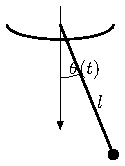
\includegraphics[width=0.3\textwidth]{figuras/pendulo.pdf}
        \caption{El péndulo del Ejercicio~153.}
    \end{figure}

    \begin{ejercicio}[Movimiento periódico de un resorte sin amortiguamiento]
        Encuentre la solución general de (3), que describe el movimiento periódico de un resorte, ignorando las fuerzas de fricción.
    \end{ejercicio}

    \begin{ejercicio}[Movimiento periódico de un resorte con amortiguamiento]
        El movimiento periódico ideal descrito por las soluciones de (3) se debe a que se ignoran las fuerzas de fricción. En realidad, sin embargo, existe una fuerza de fricción que actúa sobre el movimiento, proporcional a la rapidez del movimiento, pero que actúa en dirección opuesta. A esta modificación de (3), que da cuenta de la fuerza de fricción llamada \textbf{fuerza de amortiguamiento}, se le da por
        \begin{equation*}
            my''+ry'+ky=0,
        \end{equation*}
        donde $r>0$ es la constante de proporcionalidad.
        \begin{enumerate}[label=(\alph*)]
            \item Encuentre la solución general de esta ecuación.
            \item Encuentre la única solución de (a) que satisface las condiciones iniciales $y(0)=0$ y $y'(0)=v_0$, la velocidad inicial.
            \item Para $y(t)$ como en (b), muestre que la amplitud de la oscilación decrece a cero; es decir, pruebe que $\lim_{t\to\infty}y(t)=0$.
        \end{enumerate}
    \end{ejercicio}

    \begin{ejercicio}
        En nuestro estudio de las ecuaciones diferenciales, hemos considerado las soluciones como funciones de valores complejos, aun cuando las funciones útiles para describir el movimiento físico son de valores reales. Justifique este enfoque.
    \end{ejercicio}

    \begin{ejercicio}
        Las siguientes partes, que no involucran álgebra lineal, se incluyen por completitud.
        \begin{enumerate}[label=(\alph*)]
            \item Pruebe el Teorema~2.27. \textit{Sugerencia:} Use inducción matemática sobre el número de derivadas que posee una solución.
            \item Para cualesquiera $c,d\in\C$, pruebe que
            \begin{equation*}
                e^{c+d}=e^ce^d \qquad\text{y}\qquad e^{-c}=\frac{1}{e^c}.
            \end{equation*}
            \item Pruebe el Teorema~2.28.
            \item Pruebe el Teorema~2.29.
            \item Pruebe la regla del producto para derivar funciones de valores complejos de una variable real: para cualesquiera funciones derivables $x$ y $y$ en $\mathcal{F}(\R,\C)$, el producto $xy$ es derivable y
            \begin{equation*}
                (xy)'=x'y+xy'.
            \end{equation*}
            \textit{Sugerencia:} Aplique las reglas de derivación a las partes real e imaginaria de $xy$.
            \item Pruebe que, si $x\in\mathcal{F}(\R,\C)$ y $x'=0$, entonces $x$ es una función constante.
        \end{enumerate}
    \end{ejercicio}

    \chapter{Operaciones elementales y sistemas de ecuaciones lineales}

    Como vimos en el Capítulo~1, los sistemas de ecuaciones lineales surgen de manera natural cuando queremos saber si un vector dado puede expresarse como combinación lineal de otros vectores. Ilustramos allí un método para resolver sistemas de ecuaciones lineales, en el que se usaron ciertas operaciones para simplificar el sistema hasta obtener uno cuya solución es evidente. En este capítulo abordamos estas operaciones desde el punto de vista de las matrices, obteniendo así un método computacional para resolver sistemas de ecuaciones lineales generales, así como para calcular el rango de una transformación lineal y la inversa de una matriz.

    \section{Operaciones elementales y matrices elementales}

    En esta sección definimos las operaciones elementales que se usan a lo largo del capítulo. En secciones posteriores, usamos estas operaciones para obtener métodos computacionales sencillos para determinar el rango de una transformación lineal y la solución de un sistema de ecuaciones lineales. Existen dos tipos de operaciones elementales sobre matrices: operaciones de renglón y operaciones de columna. Como veremos, las operaciones de renglón son más útiles. Surgen de las tres operaciones que pueden usarse para eliminar variables en un sistema de ecuaciones lineales.

    \begin{definicion}[Operación elemental]
        Sea $A$ una matriz $m\times n$. Cualquiera de las siguientes tres operaciones sobre los renglones [columnas] de $A$ se llama una \textbf{operación elemental de renglón} [\textbf{columna}]:
        \begin{enumerate}
            \item[(1)] intercambiar cualesquiera dos renglones [columnas] de $A$;
            \item[(2)] multiplicar cualquier renglón [columna] de $A$ por un escalar no nulo;
            \item[(3)] sumar a cualquier renglón [columna] de $A$ un múltiplo escalar de otro renglón [columna].
        \end{enumerate}
        A cualquiera de estas tres operaciones se le llama una \textbf{operación elemental}. Las operaciones elementales son de \textbf{tipo 1}, \textbf{tipo 2}, o \textbf{tipo 3}, según se obtengan mediante (1), (2), o (3), respectivamente.
    \end{definicion}

    \begin{ejemplo}
        Sea
        \begin{equation*}
            A=\begin{pmatrix}1&2&3&4\\2&1&-1&3\\4&0&1&2\end{pmatrix}.
        \end{equation*}
        Intercambiar el segundo renglón de $A$ con el primero es un ejemplo de una operación elemental de renglón de tipo $1$. La matriz resultante es
        \begin{equation*}
            B=\begin{pmatrix}2&1&-1&3\\1&2&3&4\\4&0&1&2\end{pmatrix}.
        \end{equation*}
        Multiplicar la segunda columna de $A$ por $3$ es un ejemplo de una operación elemental de columna de tipo $2$. La matriz resultante es
        \begin{equation*}
            C=\begin{pmatrix}1&6&3&4\\2&3&-1&3\\4&0&1&2\end{pmatrix}.
        \end{equation*}
        Sumar $4$ veces el tercer renglón de $A$ al primer renglón es un ejemplo de una operación elemental de renglón de tipo $3$. En este caso, la matriz resultante es
        \begin{equation*}
            M=\begin{pmatrix}17&2&7&12\\2&1&-1&3\\4&0&1&2\end{pmatrix}.
        \end{equation*}
    \end{ejemplo}

    Notemos que, si una matriz $Q$ puede obtenerse de una matriz $P$ mediante una operación elemental de renglón, entonces $P$ puede obtenerse de $Q$ mediante una operación elemental de renglón del mismo tipo. (Véase el Ejercicio~8.) Así, en el ejemplo anterior, $A$ puede obtenerse de $M$ sumando $-4$ veces el tercer renglón de $M$ al primer renglón de $M$.

    \begin{definicion}[Matriz elemental]
        Una \textbf{matriz elemental} $n\times n$ es una matriz que se obtiene al realizar una operación elemental sobre $I_n$. Se dice que la matriz elemental es de \textbf{tipo 1}, \textbf{2}, o \textbf{3} según la operación elemental realizada sobre $I_n$ sea de tipo 1, 2, o 3, respectivamente.
    \end{definicion}

    Por ejemplo, intercambiar los primeros dos renglones de $I_3$ produce la matriz elemental
    \begin{equation*}
        E=\begin{pmatrix}0&1&0\\1&0&0\\0&0&1\end{pmatrix}.
    \end{equation*}
    Notemos que $E$ también puede obtenerse intercambiando las primeras dos columnas de $I_3$. De hecho, toda matriz elemental puede obtenerse de al menos dos maneras —ya sea realizando una operación elemental de renglón sobre $I_n$, o realizando una operación elemental de columna sobre $I_n$. (Véase el Ejercicio~4.) De manera análoga,
    \begin{equation*}
        \begin{pmatrix}1&0&-2\\0&1&0\\0&0&1\end{pmatrix}
    \end{equation*}
    es una matriz elemental, ya que puede obtenerse de $I_3$ mediante una operación elemental de columna de tipo 3 (sumando $-2$ veces la primera columna de $I_3$ a la tercera columna) o mediante una operación elemental de renglón de tipo 3 (sumando $-2$ veces el tercer renglón a el primer renglón).

    Nuestro primer teorema muestra que realizar una operación elemental de renglón sobre una matriz equivale a multiplicar la matriz por una matriz elemental.

    \begin{teorema}
        Sea $A\in M_{m\times n}(F)$, y supongamos que $B$ se obtiene de $A$ realizando una operación elemental de renglón [columna]. Entonces existe una matriz elemental $E$, de tamaño $m\times m$ [$n\times n$], tal que $B=EA$ [$B=AE$]. De hecho, $E$ se obtiene de $I_m$ [$I_n$] realizando la misma operación elemental de renglón [columna] que la que se realizó sobre $A$ para obtener $B$. Recíprocamente, si $E$ es una matriz elemental $m\times m$ [$n\times n$], entonces $EA$ [$AE$] es la matriz que se obtiene de $A$ realizando la misma operación elemental de renglón [columna] que la que produce a $E$ a partir de $I_m$ [$I_n$].
    \end{teorema}

    \begin{proof}
        Probamos el resultado para operaciones de renglón; el caso de operaciones de columna se sigue de este mediante el uso de la transpuesta, como se explica al final de la demostración.

        Sea $E$ la matriz elemental $m\times m$ que se obtiene de $I_m$ realizando una operación elemental de renglón dada, y veamos que, para \textit{cualquier} matriz $A\in M_{m\times n}(F)$, la matriz $EA$ coincide con la matriz que se obtiene de $A$ al realizar esa misma operación de renglón. Esto establece simultáneamente ambas direcciones del teorema (pues la matriz $B$ del enunciado directo es, por definición, el resultado de aplicar la operación a $A$; y el enunciado recíproco es exactamente esta misma afirmación).

        \textit{Tipo 1} (intercambiar los renglones $p$ y $q$, con $p\neq q$). Aquí $E$ es la matriz que se obtiene de $I_m$ intercambiando sus renglones $p$ y $q$; así $E_{ik}=\delta_{ik}$ si $i\neq p,q$, mientras que $E_{pk}=\delta_{qk}$ y $E_{qk}=\delta_{pk}$. Para $i\neq p,q$,
        \begin{equation*}
            (EA)_{ij}=\sum_{k=1}^{m}E_{ik}A_{kj}=\sum_{k=1}^{m}\delta_{ik}A_{kj}=A_{ij},
        \end{equation*}
        así que el renglón $i$ de $EA$ coincide con el renglón $i$ de $A$. Además,
        \begin{equation*}
            (EA)_{pj}=\sum_{k=1}^{m}\delta_{qk}A_{kj}=A_{qj} \qquad\text{y}\qquad (EA)_{qj}=\sum_{k=1}^{m}\delta_{pk}A_{kj}=A_{pj}.
        \end{equation*}
        Así $EA$ es precisamente la matriz que se obtiene de $A$ al intercambiar sus renglones $p$ y $q$.

        \textit{Tipo 2} (multiplicar el renglón $p$ por un escalar no nulo $c$). Aquí $E_{ik}=\delta_{ik}$ para $i\neq p$, y $E_{pk}=c\delta_{pk}$. Para $i\neq p$, $(EA)_{ij}=A_{ij}$ como antes; y
        \begin{equation*}
            (EA)_{pj}=\sum_{k=1}^{m}c\delta_{pk}A_{kj}=cA_{pj}.
        \end{equation*}
        Así $EA$ es la matriz que se obtiene de $A$ al multiplicar su renglón $p$ por $c$.

        \textit{Tipo 3} (sumar $c$ veces el renglón $q$ al renglón $p$, con $p\neq q$). Aquí $E_{ik}=\delta_{ik}$ para $i\neq p$, y $E_{pk}=\delta_{pk}+c\delta_{qk}$. Para $i\neq p$, de nuevo $(EA)_{ij}=A_{ij}$; y
        \begin{equation*}
            (EA)_{pj}=\sum_{k=1}^{m}(\delta_{pk}+c\delta_{qk})A_{kj}=A_{pj}+cA_{qj}.
        \end{equation*}
        Así $EA$ es la matriz que se obtiene de $A$ al sumar $c$ veces su renglón $q$ al renglón $p$.

        Esto establece el teorema para operaciones de renglón. Para operaciones de columna, supongamos que $B$ se obtiene de $A$ mediante una operación elemental de columna. Notemos que esta misma operación, aplicada a los \textit{renglones} de $A^t$ en lugar de a las columnas de $A$, produce precisamente $B^t$ (intercambiar las columnas $p,q$ de $A$ corresponde a intercambiar los renglones $p,q$ de $A^t$; multiplicar la columna $p$ de $A$ por $c$ corresponde a multiplicar el renglón $p$ de $A^t$ por $c$; y sumar $c$ veces la columna $q$ de $A$ a la columna $p$ corresponde a sumar $c$ veces el renglón $q$ de $A^t$ al renglón $p$). Por el caso de renglones ya probado, existe una matriz elemental $F$ (obtenida de $I_n$ mediante la operación de renglón correspondiente) tal que $B^t=FA^t$. Tomando transpuestas, $B=(FA^t)^t=AF^t$. Como $F^t$ es, por construcción, la matriz que se obtiene de $I_n^t=I_n$ realizando la operación de columna original (pues transponer intercambia los papeles de renglón y columna en la operación que define a $F$), $E:=F^t$ es la matriz elemental buscada, y $B=AE$.
    \end{proof}

    El siguiente ejemplo ilustra el uso del teorema anterior.

    \begin{ejemplo}
        Consideremos las matrices $A$ y $B$ del ejemplo anterior. En este caso, $B$ se obtiene de $A$ intercambiando los primeros dos renglones de $A$. Realizando esta misma operación sobre $I_3$, obtenemos la matriz elemental
        \begin{equation*}
            E=\begin{pmatrix}0&1&0\\1&0&0\\0&0&1\end{pmatrix}.
        \end{equation*}
        Notemos que $EA=B$.

        En la segunda parte del ejemplo anterior, $C$ se obtiene de $A$ multiplicando la segunda columna de $A$ por $3$. Realizando esta misma operación sobre $I_4$, obtenemos la matriz elemental
        \begin{equation*}
            E=\begin{pmatrix}1&0&0&0\\0&3&0&0\\0&0&1&0\\0&0&0&1\end{pmatrix}.
        \end{equation*}
        Observemos que $AE=C$.
    \end{ejemplo}

    Es un hecho útil que la inversa de una matriz elemental es también una matriz elemental.

    \begin{teorema}
        Las matrices elementales son invertibles, y la inversa de una matriz elemental es una matriz elemental del mismo tipo.
    \end{teorema}

    \begin{proof}
        Sea $E$ una matriz elemental $n\times n$. Entonces $E$ se obtiene mediante una operación elemental de renglón sobre $I_n$. Invirtiendo los pasos usados para transformar $I_n$ en $E$, podemos transformar $E$ de vuelta en $I_n$. El resultado es que $I_n$ puede obtenerse de $E$ mediante una operación elemental de renglón del mismo tipo. Por el teorema anterior, existe una matriz elemental $\overline{E}$ tal que $\overline{E}E=I_n$. Por tanto, por el Ejercicio~90 de la Sección~2.4, $E$ es invertible y $E^{-1}=\overline{E}$.
    \end{proof}

    \begin{ejercicio}
        Etiquete las siguientes afirmaciones como verdaderas o falsas.
        \begin{enumerate}[label=(\alph*)]
            \item Una matriz elemental siempre es cuadrada.
            \item Las únicas entradas de una matriz elemental son ceros y unos.
            \item La matriz identidad $n\times n$ es una matriz elemental.
            \item El producto de dos matrices elementales $n\times n$ es una matriz elemental.
            \item La inversa de una matriz elemental es una matriz elemental.
            \item La suma de dos matrices elementales $n\times n$ es una matriz elemental.
            \item La transpuesta de una matriz elemental es una matriz elemental.
            \item Si $B$ es una matriz que puede obtenerse al realizar una operación elemental de renglón sobre una matriz $A$, entonces $B$ también puede obtenerse realizando una operación elemental de columna sobre $A$.
            \item Si $B$ es una matriz que puede obtenerse al realizar una operación elemental de renglón sobre una matriz $A$, entonces $A$ puede obtenerse realizando una operación elemental de renglón sobre $B$.
        \end{enumerate}
    \end{ejercicio}

    \begin{ejercicio}
        Sean
        \begin{equation*}
            A=\begin{pmatrix}1&2&3\\1&0&1\\1&-1&1\end{pmatrix}, \quad B=\begin{pmatrix}1&0&3\\1&-2&1\\1&-3&1\end{pmatrix}, \quad\text{y}\quad C=\begin{pmatrix}1&0&3\\0&-2&-2\\1&-3&1\end{pmatrix}.
        \end{equation*}
        Encuentre una operación elemental que transforme $A$ en $B$, y una operación elemental que transforme $B$ en $C$. Mediante varias operaciones adicionales, transforme $C$ en $I_3$.
    \end{ejercicio}

    \begin{ejercicio}
        Use la demostración del teorema anterior para obtener la inversa de cada una de las siguientes matrices elementales.
        \begin{enumerate}[label=(\alph*)]
            \item $\begin{pmatrix}0&0&1\\0&1&0\\1&0&0\end{pmatrix}$
            \item $\begin{pmatrix}1&0&0\\0&3&0\\0&0&1\end{pmatrix}$
            \item $\begin{pmatrix}1&0&0\\0&1&0\\-2&0&1\end{pmatrix}$
        \end{enumerate}
    \end{ejercicio}

    \begin{ejercicio}
        Pruebe la afirmación hecha en el texto: cualquier matriz elemental $n\times n$ puede obtenerse de al menos dos maneras —ya sea realizando una operación elemental de renglón sobre $I_n$, o realizando una operación elemental de columna sobre $I_n$.
    \end{ejercicio}

    \begin{ejercicio}
        Pruebe que $E$ es una matriz elemental si y solo si $E^t$ lo es.
    \end{ejercicio}

    \begin{ejercicio}
        Sea $A$ una matriz $m\times n$. Pruebe que, si $B$ puede obtenerse de $A$ mediante una operación elemental de renglón [columna], entonces $B^t$ puede obtenerse de $A^t$ mediante la operación elemental de columna [renglón] correspondiente.
    \end{ejercicio}

    \begin{ejercicio}
        Pruebe el Teorema~3.1.
    \end{ejercicio}

    \begin{ejercicio}
        Pruebe que, si una matriz $Q$ puede obtenerse de una matriz $P$ mediante una operación elemental de renglón, entonces $P$ puede obtenerse de $Q$ mediante una operación elemental de renglón del mismo tipo. \textit{Sugerencia:} Trate cada tipo de operación elemental de renglón por separado.
    \end{ejercicio}

    \begin{ejercicio}
        Pruebe que cualquier operación elemental de renglón [columna] de tipo 1 puede obtenerse mediante una sucesión de tres operaciones elementales de renglón [columna] de tipo 3, seguidas de una de tipo 2.
    \end{ejercicio}

    \begin{ejercicio}
        Pruebe que cualquier operación elemental de renglón [columna] de tipo 2 puede obtenerse \textit{dividiendo} algún renglón [columna] entre un escalar no nulo.
    \end{ejercicio}

    \begin{ejercicio}
        Pruebe que cualquier operación elemental de renglón [columna] de tipo 3 puede obtenerse \textit{restando} un múltiplo de algún renglón [columna] de otro renglón [columna].
    \end{ejercicio}

    \begin{ejercicio}
        Sea $A$ una matriz $m\times n$. Pruebe que existe una sucesión de operaciones elementales de renglón de tipos 1 y 3 que transforma $A$ en una matriz triangular superior.
    \end{ejercicio}

    \section{El rango de una matriz y las inversas de matrices}

    En esta sección definimos el \textit{rango} de una matriz. Usamos después operaciones elementales para calcular el rango de una matriz y de una transformación lineal. La sección concluye con un procedimiento para calcular la inversa de una matriz invertible.

    \begin{definicion}[Rango de una matriz]
        Si $A\in M_{m\times n}(F)$, definimos el \textbf{rango} de $A$, denotado $\rg(A)$, como el rango de la transformación lineal $L_A:F^n\to F^m$.
    \end{definicion}

    Muchos resultados sobre el rango de una matriz se siguen de inmediato de los hechos correspondientes sobre una transformación lineal. Un resultado importante de este tipo, que se sigue del hecho~3 de la Sección~2.4 y del corolario~2 al Teorema~2.18, es que \textit{una matriz $n\times n$ es invertible si y solo si su rango es $n$}.

    Toda matriz $A$ es la representación matricial de la transformación lineal $L_A$ respecto a las bases estándar adecuadas. Así el rango de la transformación lineal $L_A$ es el mismo que el rango de una de sus representaciones matriciales, a saber, $A$. El siguiente teorema extiende este hecho a cualquier representación matricial de cualquier transformación lineal definida sobre espacios vectoriales de dimensión finita.

    \begin{teorema}
        Sea $T:V\to W$ una transformación lineal entre espacios vectoriales de dimensión finita, y sean $\BB$ y $\gamma$ bases ordenadas para $V$ y $W$, respectivamente. Entonces $\rg(T)=\rg\big([T]_\BB^\gamma\big)$.
    \end{teorema}

    \begin{proof}
        Esta es una reformulación del Ejercicio~98 de la Sección~2.4.
    \end{proof}

    Ahora que el problema de encontrar el rango de una transformación lineal se ha reducido al problema de encontrar el rango de una matriz, necesitamos un resultado que nos permita realizar operaciones que preserven el rango sobre matrices. El siguiente teorema y su corolario nos dicen cómo hacerlo.

    \begin{teorema}
        Sea $A$ una matriz $m\times n$. Si $P$ y $Q$ son matrices invertibles $m\times m$ y $n\times n$, respectivamente, entonces:
        \begin{enumerate}[label=(\alph*)]
            \item $\rg(AQ)=\rg(A)$.
            \item $\rg(PA)=\rg(A)$,
        \end{enumerate}
        y, por tanto,
        \begin{enumerate}[label=(\alph*), start=3]
            \item $\rg(PAQ)=\rg(A)$.
        \end{enumerate}
    \end{teorema}

    \begin{proof}
        Primero observemos que
        \begin{equation*}
            \Im(L_{AQ})=\Im(L_AL_Q)=L_A\big(L_Q(F^n)\big)=L_A\big(\Im(L_Q)\big)=L_A(F^n)=\Im(L_A)
        \end{equation*}
        ya que $L_Q$ es sobreyectiva. Por tanto
        \begin{equation*}
            \rg(AQ)=\dim\big(\Im(L_{AQ})\big)=\dim\big(\Im(L_A)\big)=\rg(A).
        \end{equation*}
        Esto establece (a).

        Para establecer (b), notemos que, como $P$ es invertible, $L_P$ es inyectiva; así, para $x\in F^n$,
        \begin{equation*}
            L_{PA}(x)=0 \iff L_P\big(L_A(x)\big)=0 \iff L_A(x)=0,
        \end{equation*}
        de donde $\ker(L_{PA})=\ker(L_A)$, y por tanto $\nul(PA)=\nul(A)$. Por el teorema de la dimensión, aplicado a $L_{PA}$ y a $L_A$ (ambas definidas sobre $F^n$),
        \begin{equation*}
            \rg(PA)=n-\nul(PA)=n-\nul(A)=\rg(A).
        \end{equation*}

        Finalmente, aplicando (a) y (b), tenemos
        \begin{equation*}
            \rg(PAQ)=\rg(PA)=\rg(A).
        \end{equation*}
    \end{proof}

    \begin{corolario}
        Las operaciones elementales de renglón y columna sobre una matriz preservan el rango.
    \end{corolario}

    \begin{proof}
        Si $B$ se obtiene de una matriz $A$ mediante una operación elemental de renglón, entonces existe una matriz elemental $E$ tal que $B=EA$. Por el Teorema~3.2, $E$ es invertible, y por tanto $\rg(B)=\rg(A)$ por el teorema anterior. La prueba de que las operaciones elementales de columna preservan el rango se deja como ejercicio (véase el Ejercicio~21): es análoga, usando que $B=AE$ para una matriz elemental $E$ (invertible) y aplicando el inciso (a) del teorema anterior.
    \end{proof}

    Ahora que tenemos una clase de operaciones matriciales que preservan el rango, necesitamos una manera de examinar una matriz transformada para determinar su rango. El siguiente teorema es el primero de varios en esta dirección.

    \begin{teorema}
        El rango de cualquier matriz es igual al número máximo de sus columnas linealmente independientes; es decir, el rango de una matriz es la dimensión del subespacio generado por sus columnas.
    \end{teorema}

    \begin{proof}
        Para cualquier $A\in M_{m\times n}(F)$,
        \begin{equation*}
            \rg(A)=\rg(L_A)=\dim\big(\Im(L_A)\big).
        \end{equation*}
        Sea $\BB$ la base ordenada estándar para $F^n$. Entonces $\BB$ genera a $F^n$, y por tanto, por el Teorema~2.2,
        \begin{equation*}
            \Im(L_A)=\gen{L_A(\BB)}=\gen{\{L_A(e_1),L_A(e_2),\dots,L_A(e_n)\}}.
        \end{equation*}
        Pero, para cualquier $j$, ya hemos visto en el Teorema~2.13(b) que $L_A(e_j)=Ae_j=a_j$, donde $a_j$ es la $j$-ésima columna de $A$. Así
        \begin{equation*}
            \Im(L_A)=\gen{\{a_1,a_2,\dots,a_n\}}.
        \end{equation*}
        Por tanto
        \begin{equation*}
            \rg(A)=\dim\big(\Im(L_A)\big)=\dim\big(\gen{\{a_1,a_2,\dots,a_n\}}\big).
        \end{equation*}
    \end{proof}

    \begin{ejemplo}
        Sea
        \begin{equation*}
            A=\begin{pmatrix}1&0&1\\0&1&1\\1&0&1\end{pmatrix}.
        \end{equation*}
        Observemos que la primera y segunda columnas de $A$ son linealmente independientes, y que la tercera columna es combinación lineal de las primeras dos. Así
        \begin{equation*}
            \rg(A)=\dim\left(\gen{\left\{\begin{pmatrix}1\\0\\1\end{pmatrix},\begin{pmatrix}0\\1\\0\end{pmatrix},\begin{pmatrix}1\\1\\1\end{pmatrix}\right\}}\right)=2.
        \end{equation*}
    \end{ejemplo}

    Para calcular el rango de una matriz $A$, con frecuencia resulta útil posponer el uso del Teorema~3.5 hasta que $A$ se haya modificado adecuadamente mediante operaciones elementales de renglón y columna apropiadas, de modo que el número de columnas linealmente independientes sea evidente. El corolario al Teorema~3.4 garantiza que el rango de la matriz modificada es el mismo que el rango de $A$. Una de tales modificaciones de $A$ puede obtenerse usando operaciones elementales de renglón y columna para introducir entradas cero. El siguiente ejemplo ilustra este procedimiento.

    \begin{ejemplo}
        Sea
        \begin{equation*}
            A=\begin{pmatrix}1&2&1\\1&0&3\\1&1&2\end{pmatrix}.
        \end{equation*}
        Si restamos el primer renglón de $A$ de los renglones 2 y 3 (operaciones elementales de renglón de tipo 3), el resultado es
        \begin{equation*}
            \begin{pmatrix}1&2&1\\0&-2&2\\0&-1&1\end{pmatrix}.
        \end{equation*}
        Si ahora restamos dos veces la primera columna de la segunda, y restamos la primera columna de la tercera (operaciones elementales de columna de tipo 3), obtenemos
        \begin{equation*}
            \begin{pmatrix}1&0&0\\0&-2&2\\0&-1&1\end{pmatrix}.
        \end{equation*}
        Es ahora evidente que el número máximo de columnas linealmente independientes de esta matriz es $2$. Por tanto el rango de $A$ es $2$.
    \end{ejemplo}

    El siguiente teorema usa este proceso para transformar una matriz en una forma particularmente sencilla. El poder de este teorema puede apreciarse en sus corolarios.

    \begin{teorema}
        Sea $A$ una matriz $m\times n$ de rango $r$. Entonces $r\leq m$, $r\leq n$, y, mediante un número finito de operaciones elementales de renglón y columna, $A$ puede transformarse en la matriz
        \begin{equation*}
            D=\begin{pmatrix}I_r&O_1\\O_2&O_3\end{pmatrix},
        \end{equation*}
        donde $O_1$, $O_2$ y $O_3$ son matrices cero. Así $D_{ii}=1$ para $i\leq r$, y $D_{ij}=0$ en cualquier otro caso.
    \end{teorema}

    Los Teoremas~3.6 y sus corolarios son bastante importantes. Su demostración, aunque fácil de entender, resulta tediosa de leer. Como ayuda para seguirla, primero consideramos un ejemplo.

    \begin{ejemplo}
        Consideremos la matriz
        \begin{equation*}
            A=\begin{pmatrix}0&2&4&2&2\\4&4&4&8&0\\8&2&0&10&2\\6&3&2&9&1\end{pmatrix}.
        \end{equation*}
        Mediante una sucesión de operaciones elementales de renglón y columna, podemos transformar $A$ en una matriz $D$ como en el Teorema~3.6. Listamos muchas de las matrices intermedias, pero en varias ocasiones una matriz se transforma de la anterior mediante varias operaciones elementales. El número sobre cada flecha indica cuántas operaciones elementales están involucradas. Intente identificar la naturaleza de cada operación elemental (renglón o columna, y tipo) en las siguientes transformaciones de matrices.
        \begin{equation*}
            \begin{pmatrix}0&2&4&2&2\\4&4&4&8&0\\8&2&0&10&2\\6&3&2&9&1\end{pmatrix}
            \xrightarrow{1}
            \begin{pmatrix}4&4&4&8&0\\0&2&4&2&2\\8&2&0&10&2\\6&3&2&9&1\end{pmatrix}
            \xrightarrow{1}
            \begin{pmatrix}1&1&1&2&0\\0&2&4&2&2\\8&2&0&10&2\\6&3&2&9&1\end{pmatrix}
            \xrightarrow{2}
        \end{equation*}
        \begin{equation*}
            \begin{pmatrix}1&1&1&2&0\\0&2&4&2&2\\0&-6&-8&-6&2\\0&-3&-4&-3&1\end{pmatrix}
            \xrightarrow{3}
            \begin{pmatrix}1&0&0&0&0\\0&2&4&2&2\\0&-6&-8&-6&2\\0&-3&-4&-3&1\end{pmatrix}
            \xrightarrow{1}
            \begin{pmatrix}1&0&0&0&0\\0&1&2&1&1\\0&-6&-8&-6&2\\0&-3&-4&-3&1\end{pmatrix}
            \xrightarrow{2}
        \end{equation*}
        \begin{equation*}
            \begin{pmatrix}1&0&0&0&0\\0&1&2&1&1\\0&0&4&0&8\\0&0&2&0&4\end{pmatrix}
            \xrightarrow{3}
            \begin{pmatrix}1&0&0&0&0\\0&1&0&0&0\\0&0&4&0&8\\0&0&2&0&4\end{pmatrix}
            \xrightarrow{1}
            \begin{pmatrix}1&0&0&0&0\\0&1&0&0&0\\0&0&1&0&2\\0&0&2&0&4\end{pmatrix}
            \xrightarrow{1}
        \end{equation*}
        \begin{equation*}
            \begin{pmatrix}1&0&0&0&0\\0&1&0&0&0\\0&0&1&0&2\\0&0&0&0&0\end{pmatrix}
            \xrightarrow{1}
            \begin{pmatrix}1&0&0&0&0\\0&1&0&0&0\\0&0&1&0&0\\0&0&0&0&0\end{pmatrix}=D.
        \end{equation*}
        Por el corolario al Teorema~3.4, $\rg(A)=\rg(D)$. Claramente, sin embargo, $\rg(D)=3$; así $\rg(A)=3$.
    \end{ejemplo}

    Notemos que las primeras dos operaciones elementales del ejemplo anterior producen un $1$ en la posición $(1,1)$, y las siguientes operaciones producen ceros en todas las entradas del primer renglón y de la primera columna, salvo en la posición $(1,1)$. Las operaciones elementales subsecuentes no cambian el primer renglón ni la primera columna. Con este ejemplo en mente, procedemos con la demostración del Teorema~3.6.

    \begin{proof}[Demostración del Teorema~3.6]
        Si $A$ es la matriz cero, $r=0$ por el Ejercicio~15. En este caso, la conclusión se sigue tomando $D=A$.

        Supongamos ahora que $A\neq O$ y $r=\rg(A)$; entonces $r>0$. La demostración es por inducción matemática sobre $m$, el número de renglones de $A$.

        Supongamos que $m=1$. Mediante a lo más una operación elemental de columna de tipo 1 y a lo más una operación elemental de columna de tipo 2, $A$ puede transformarse en una matriz con un $1$ en la posición $(1,1)$. Mediante a lo más $n-1$ operaciones elementales de columna de tipo 3, esta matriz puede a su vez transformarse en la matriz
        \begin{equation*}
            \begin{pmatrix}1&0&\cdots&0\end{pmatrix}.
        \end{equation*}
        Notemos que existe una columna linealmente independiente en $D$. Así $\rg(D)=\rg(A)=1$ por el corolario al Teorema~3.4 y por el Teorema~3.5. Así el teorema queda establecido para $m=1$.

        Supongamos ahora que el teorema es válido para cualquier matriz con a lo más $m-1$ renglones (para algún $m>1$). Debemos probar que el teorema es válido para cualquier matriz con $m$ renglones.

        Supongamos que $A$ es cualquier matriz $m\times n$. Si $n=1$, el Teorema~3.6 puede establecerse de manera análoga a como se hizo para $m=1$ (véase el Ejercicio~22).

        Supongamos ahora que $n>1$. Como $A\neq O$, $A_{ij}\neq 0$ para algunos $i,j$. Mediante a lo más una operación elemental de renglón y a lo más una operación elemental de columna (cada una de tipo 1), podemos mover la entrada no nula a la posición $(1,1)$ (tal como se hizo en el Ejemplo~5). Mediante a lo más una operación elemental de columna adicional (de tipo 2), podemos asegurar un $1$ en la posición $(1,1)$. (Véase la segunda operación en el Ejemplo~5.) Mediante a lo más $m-1$ operaciones elementales de renglón de tipo 3 y a lo más $n-1$ operaciones elementales de columna de tipo 3, podemos eliminar todas las entradas no nulas del primer renglón y de la primera columna, con excepción del $1$ en la posición $(1,1)$. (En el Ejemplo~5, usamos dos operaciones de renglón y tres de columna para hacer esto.)

        Así, mediante un número finito de operaciones elementales, $A$ puede transformarse en una matriz
        \begin{equation*}
            B=\left(\begin{array}{c|ccc}1&0&\cdots&0\\\hline 0&&&\\\vdots&&B'&\\0&&&\end{array}\right),
        \end{equation*}
        donde $B'$ es una matriz $(m-1)\times(n-1)$. En el Ejemplo~5, por ejemplo,
        \begin{equation*}
            B'=\begin{pmatrix}2&4&2&2\\-6&-8&-6&2\\-3&-4&-3&1\end{pmatrix}.
        \end{equation*}

        Por el Ejercicio~23, $B'$ tiene rango uno menos que el de $B$. Como $\rg(A)=\rg(B)=r$, $\rg(B')=r-1$. Por tanto $r-1\leq m-1$ y $r-1\leq n-1$ por la hipótesis de inducción. Por tanto $r\leq m$ y $r\leq n$.

        Además, por la hipótesis de inducción, $B'$ puede transformarse mediante un número finito de operaciones elementales de renglón y columna en la matriz $(m-1)\times(n-1)$ $D'$ tal que
        \begin{equation*}
            D'=\begin{pmatrix}I_{r-1}&O_4\\O_5&O_6\end{pmatrix},
        \end{equation*}
        donde $O_4$, $O_5$ y $O_6$ son matrices cero. Es decir, $D'$ consiste enteramente de ceros, salvo sus primeras $r-1$ entradas diagonales, las cuales son unos. Sea
        \begin{equation*}
            D=\left(\begin{array}{c|ccc}1&0&\cdots&0\\\hline 0&&&\\\vdots&&D'&\\0&&&\end{array}\right).
        \end{equation*}

        Vemos que el teorema se sigue una vez que mostremos que $D$ puede obtenerse de $B$ mediante un número finito de operaciones elementales de renglón y columna. Sin embargo, esto se sigue aplicando repetidamente el Ejercicio~24.

        Así, como $A$ puede transformarse en $B$, y $B$ puede transformarse en $D$, cada una mediante un número finito de operaciones elementales, $A$ puede transformarse en $D$ mediante un número finito de operaciones elementales.

        Finalmente, como $D'$ contiene unos como sus primeras $r-1$ entradas diagonales, $D$ contiene unos como sus primeras $r$ entradas diagonales y ceros en las demás posiciones. Esto establece el teorema.
    \end{proof}

    \begin{corolario}
        Sea $A$ una matriz $m\times n$ de rango $r$. Entonces existen matrices invertibles $B$ y $C$, de tamaños $m\times m$ y $n\times n$, respectivamente, tales que $D=BAC$, donde
        \begin{equation*}
            D=\begin{pmatrix}I_r&O_1\\O_2&O_3\end{pmatrix}
        \end{equation*}
        es la matriz $m\times n$ en la cual $O_1$, $O_2$ y $O_3$ son matrices cero.
    \end{corolario}

    \begin{proof}
        Por el Teorema~3.6, $A$ puede transformarse mediante un número finito de operaciones elementales de renglón y columna en la matriz $D$. Podemos apelar al Teorema~3.1 cada vez que realizamos una operación elemental. Así existen matrices elementales $m\times m$, $E_1,E_2,\dots,E_p$, y matrices elementales $n\times n$, $G_1,G_2,\dots,G_q$, tales que
        \begin{equation*}
            D=E_pE_{p-1}\cdots E_2E_1AG_1G_2\cdots G_q.
        \end{equation*}
        Por el Teorema~3.2, cada $E_j$ y $G_j$ es invertible. Sean $B=E_pE_{p-1}\cdots E_1$ y $C=G_1G_2\cdots G_q$. Entonces $B$ y $C$ son invertibles por el Ejercicio~84 de la Sección~2.4, y $D=BAC$.
    \end{proof}

    \begin{corolario}
        Sea $A$ una matriz $m\times n$. Entonces:
        \begin{enumerate}[label=(\alph*)]
            \item $\rg(A^t)=\rg(A)$.
            \item El rango de cualquier matriz es igual al número máximo de sus renglones linealmente independientes; es decir, el rango de una matriz es la dimensión del subespacio generado por sus renglones.
            \item Los renglones y las columnas de cualquier matriz generan subespacios de la misma dimensión, numéricamente igual al rango de la matriz.
        \end{enumerate}
    \end{corolario}

    \begin{proof}
        (a) Por el corolario anterior, existen matrices invertibles $B$ y $C$ tales que $D=BAC$, donde $D$ satisface las condiciones establecidas en el corolario. Tomando transpuestas, tenemos
        \begin{equation*}
            D^t=(BAC)^t=C^tA^tB^t.
        \end{equation*}
        Como $B$ y $C$ son invertibles, también lo son $B^t$ y $C^t$ por el Ejercicio~85 de la Sección~2.4. De aquí, por el Teorema~3.4,
        \begin{equation*}
            \rg(A^t)=\rg(C^tA^tB^t)=\rg(D^t).
        \end{equation*}
        Supongamos que $r=\rg(A)$. Entonces $D^t$ es una matriz $n\times m$ con la misma forma que la matriz $D$ del Corolario~1, y por tanto $\rg(D^t)=r$ por el Teorema~3.5. Así
        \begin{equation*}
            \rg(A^t)=\rg(D^t)=r=\rg(A).
        \end{equation*}
        Esto establece (a).

        (b) Por el Teorema~3.5 aplicado a $A^t$, $\rg(A^t)$ es igual al número máximo de columnas linealmente independientes de $A^t$, es decir, al número máximo de renglones linealmente independientes de $A$ (pues las columnas de $A^t$ son, por definición, los renglones de $A$). Por (a), esto es igual a $\rg(A)$. Así el rango de $A$ es igual al número máximo de renglones linealmente independientes de $A$, es decir, a la dimensión del subespacio generado por los renglones de $A$.

        (c) Por el Teorema~3.5, la dimensión del subespacio generado por las columnas de $A$ es $\rg(A)$; y, por (b), la dimensión del subespacio generado por los renglones de $A$ es también $\rg(A)$. Así ambos subespacios tienen dimensión $\rg(A)$, numéricamente igual al rango de $A$.
    \end{proof}

    \begin{corolario}
        Toda matriz invertible es un producto de matrices elementales.
    \end{corolario}

    \begin{proof}
        Si $A$ es una matriz invertible $n\times n$, entonces $\rg(A)=n$. Por tanto, la matriz $D$ del Corolario~1 es igual a $I_n$, y existen matrices invertibles $B$ y $C$ tales que $I_n=BAC$.

        Como en la demostración del Corolario~1, notemos que $B=E_pE_{p-1}\cdots E_1$ y $C=G_1G_2\cdots G_q$, donde las $E_i$ y las $G_i$ son matrices elementales. Así
        \begin{equation*}
            A=B^{-1}I_nC^{-1}=B^{-1}C^{-1}=E_1^{-1}E_2^{-1}\cdots E_p^{-1}G_q^{-1}G_{q-1}^{-1}\cdots G_1^{-1}.
        \end{equation*}
        Las inversas de matrices elementales son, sin embargo, matrices elementales; y por tanto $A$ es el producto de matrices elementales.
    \end{proof}

    Usamos ahora el Corolario~2 para relacionar el rango de un producto de matrices con el rango de cada factor. Observemos cómo la demostración explota la relación entre el rango de una matriz y el rango de una transformación lineal.

    \begin{teorema}
        Sean $T:V\to W$ y $U:W\to Z$ transformaciones lineales entre espacios vectoriales de dimensión finita $V$, $W$ y $Z$, y sean $A$ y $B$ matrices tales que el producto $AB$ está definido. Entonces:
        \begin{enumerate}[label=(\alph*)]
            \item $\rg(UT)\leq\rg(U)$.
            \item $\rg(UT)\leq\rg(T)$.
            \item $\rg(AB)\leq\rg(A)$.
            \item $\rg(AB)\leq\rg(B)$.
        \end{enumerate}
    \end{teorema}

    \begin{proof}
        Probamos estos incisos en el orden (a), (c), (d), y (b).

        (a) Claramente $\Im(T)\subseteq W$. Por tanto
        \begin{equation*}
            \Im(UT)=UT(V)=U\big(T(V)\big)=U\big(\Im(T)\big)\subseteq U(W)=\Im(U).
        \end{equation*}
        Así
        \begin{equation*}
            \rg(UT)=\dim\big(\Im(UT)\big)\leq\dim\big(\Im(U)\big)=\rg(U).
        \end{equation*}

        (c) Por (a),
        \begin{equation*}
            \rg(AB)=\rg(L_{AB})=\rg(L_AL_B)\leq\rg(L_A)=\rg(A).
        \end{equation*}

        (d) Por (c) y el Corolario~2 al Teorema~3.6,
        \begin{equation*}
            \rg(AB)=\rg\big((AB)^t\big)=\rg(B^tA^t)\leq\rg(B^t)=\rg(B).
        \end{equation*}

        (b) Sean $\alpha$, $\BB$ y $\gamma$ bases ordenadas para $V$, $W$ y $Z$, respectivamente, y sean $A'=[U]_\BB^\gamma$ y $B'=[T]_\alpha^\BB$. Entonces $A'B'=[UT]_\alpha^\gamma$ por el Teorema~2.11. Por tanto, por el Teorema~3.3 y (d),
        \begin{equation*}
            \rg(UT)=\rg(A'B')\leq\rg(B')=\rg(T).
        \end{equation*}
    \end{proof}

    Es importante poder calcular el rango de cualquier matriz. Podemos usar el corolario al Teorema~3.4, los Teoremas~3.5 y 3.6, y el Corolario~2 al Teorema~3.6 para lograr este objetivo.

    El objetivo es realizar operaciones elementales de renglón y columna sobre una matriz para \textquotedblleft simplificarla\textquotedblright\ (de modo que la matriz transformada tenga muchas entradas cero) hasta el punto en que una simple observación nos permita determinar cuántos renglones o columnas linealmente independientes tiene la matriz, y así determinar su rango.

    \begin{ejemplo}
        (a) Sea
        \begin{equation*}
            A=\begin{pmatrix}1&2&1&1\\1&1&-1&1\end{pmatrix}.
        \end{equation*}
        Notemos que el primer y segundo renglón de $A$ son linealmente independientes, ya que uno no es múltiplo del otro. Así $\rg(A)=2$.

        (b) Sea
        \begin{equation*}
            A=\begin{pmatrix}1&3&1&1\\1&0&1&1\\0&3&0&0\end{pmatrix}.
        \end{equation*}
        En este caso, hay varias formas de proceder. Supongamos que comenzamos con una operación elemental de renglón para obtener un cero en la posición $(2,1)$. Restando el primer renglón del segundo renglón, obtenemos
        \begin{equation*}
            \begin{pmatrix}1&3&1&1\\0&-3&0&0\\0&3&0&0\end{pmatrix}.
        \end{equation*}
        Ahora notemos que el tercer renglón es un múltiplo del segundo renglón, y que el primer y segundo renglón son linealmente independientes. Así $\rg(A)=2$.

        Como método alternativo, notemos que la primera, tercera y cuarta columnas de $A$ son idénticas, y que la primera y segunda columnas de $A$ son linealmente independientes. Por tanto $\rg(A)=2$.

        (c) Sea
        \begin{equation*}
            A=\begin{pmatrix}1&2&3&1\\2&1&1&1\\1&-1&1&0\end{pmatrix}.
        \end{equation*}
        Usando operaciones elementales de renglón, podemos transformar $A$ como sigue:
        \begin{equation*}
            A\longrightarrow\begin{pmatrix}1&2&3&1\\0&-3&-5&-1\\0&-3&-2&-1\end{pmatrix}\longrightarrow\begin{pmatrix}1&2&3&1\\0&-3&-5&-1\\0&0&3&0\end{pmatrix}.
        \end{equation*}
        Es claro que la última matriz tiene tres renglones linealmente independientes y, por tanto, tiene rango $3$.
    \end{ejemplo}

    En resumen, se realizan operaciones de renglón y columna hasta que la matriz esté suficientemente simplificada de modo que sea evidente el número máximo de renglones o columnas linealmente independientes.

    \subsection*{La inversa de una matriz}

    Hemos observado que una matriz $n\times n$ es invertible si y solo si su rango es $n$. Como sabemos calcular el rango de cualquier matriz, siempre podemos probar si una matriz es invertible. Proporcionamos ahora una técnica sencilla para calcular la inversa de una matriz que utiliza operaciones elementales de renglón.

    \begin{definicion}[Matriz aumentada]
        Sean $A$ y $B$ matrices $m\times n$ y $m\times p$, respectivamente. Por la \textbf{matriz aumentada} $(A|B)$ entendemos la matriz $m\times(n+p)$, es decir, la matriz cuyas primeras $n$ columnas son las columnas de $A$, y cuyas últimas $p$ columnas son las columnas de $B$.
    \end{definicion}

    Sea $A$ una matriz invertible $n\times n$, y consideremos la matriz aumentada $n\times 2n$, $C=(A|I_n)$. Por el Ejercicio~27,
    \begin{equation*}
        A^{-1}C=(A^{-1}A|A^{-1}I_n)=(I_n|A^{-1}). \tag{1}
    \end{equation*}
    Por el Corolario~3 al Teorema~3.6, $A^{-1}$ es el producto de matrices elementales, digamos $A^{-1}=E_pE_{p-1}\cdots E_1$. Así (1) se convierte en
    \begin{equation*}
        E_pE_{p-1}\cdots E_1(A|I_n)=A^{-1}C=(I_n|A^{-1}).
    \end{equation*}
    Como multiplicar una matriz a la izquierda por una matriz elemental transforma la matriz mediante una operación elemental de renglón (Teorema~3.1), tenemos el siguiente resultado: \textit{si $A$ es una matriz invertible $n\times n$, entonces es posible transformar la matriz $(A|I_n)$ en la matriz $(I_n|A^{-1})$ mediante un número finito de operaciones elementales de renglón}.

    Recíprocamente, supongamos que $A$ es invertible y que, para alguna matriz $n\times n$ $B$, la matriz $(A|I_n)$ puede transformarse en la matriz $(I_n|B)$ mediante un número finito de operaciones elementales de renglón. Sean $E_1,E_2,\dots,E_p$ las matrices elementales asociadas con estas operaciones elementales, como en el Teorema~3.1; entonces
    \begin{equation*}
        E_pE_{p-1}\cdots E_1(A|I_n)=(I_n|B). \tag{2}
    \end{equation*}
    Sea $M=E_pE_{p-1}\cdots E_1$. Tenemos, de (2), que
    \begin{equation*}
        (MA|M)=M(A|I_n)=(I_n|B).
    \end{equation*}
    Por tanto $MA=I_n$ y $M=B$. Se sigue que $M=A^{-1}$. Así $B=A^{-1}$. Tenemos entonces el siguiente resultado: \textit{si $A$ es una matriz invertible $n\times n$, y la matriz $(A|I_n)$ se transforma en una matriz de la forma $(I_n|B)$ mediante un número finito de operaciones elementales de renglón, entonces $B=A^{-1}$}.

    Si, por otro lado, $A$ es una matriz $n\times n$ que no es invertible, entonces $\rg(A)<n$. Por tanto, cualquier intento de transformar $(A|I_n)$ en una matriz de la forma $(I_n|B)$ mediante operaciones elementales de renglón debe fallar, pues de otro modo $A$ podría transformarse en $I_n$ usando estas mismas operaciones de renglón. Esto es imposible, sin embargo, porque las operaciones elementales de renglón preservan el rango. De hecho, $A$ puede transformarse en una matriz con un renglón que contiene solamente entradas cero, dando el siguiente resultado: \textit{si $A$ es una matriz $n\times n$ que no es invertible, entonces cualquier intento de transformar $(A|I_n)$ en una matriz de la forma $(I_n|B)$ produce un renglón cuyas primeras $n$ entradas son ceros}.

    Los siguientes dos ejemplos ilustran estos comentarios.

    \begin{ejemplo}
        Determinamos si la matriz
        \begin{equation*}
            A=\begin{pmatrix}0&2&4\\2&4&2\\3&3&1\end{pmatrix}
        \end{equation*}
        es invertible, y si lo es, calculamos su inversa.

        Intentamos usar operaciones elementales de renglón para transformar
        \begin{equation*}
            (A|I)=\left(\begin{array}{ccc|ccc}0&2&4&1&0&0\\2&4&2&0&1&0\\3&3&1&0&0&1\end{array}\right)
        \end{equation*}
        en una matriz de la forma $(I|B)$. Un método para lograr esta transformación consiste en cambiar cada columna de $A$ sucesivamente, comenzando por la primera, por la columna correspondiente de $I$. Como necesitamos una entrada no nula en la posición $(1,1)$, comenzamos intercambiando los renglones 1 y 2. El resultado es
        \begin{equation*}
            \left(\begin{array}{ccc|ccc}2&4&2&0&1&0\\0&2&4&1&0&0\\3&3&1&0&0&1\end{array}\right).
        \end{equation*}
        Para colocar un $1$ en la posición $(1,1)$, debemos multiplicar el primer renglón por $\tfrac12$; esta operación produce
        \begin{equation*}
            \left(\begin{array}{ccc|ccc}1&2&1&0&\tfrac12&0\\0&2&4&1&0&0\\3&3&1&0&0&1\end{array}\right).
        \end{equation*}
        Completamos ahora el trabajo en la primera columna sumando $-3$ veces el renglón 1 al renglón 3, para obtener
        \begin{equation*}
            \left(\begin{array}{ccc|ccc}1&2&1&0&\tfrac12&0\\0&2&4&1&0&0\\0&-3&-2&0&-\tfrac32&1\end{array}\right).
        \end{equation*}
        Para cambiar la segunda columna de la matriz anterior por la segunda columna de $I$, multiplicamos el renglón 2 por $\tfrac12$ para obtener un $1$ en la posición $(2,2)$. Esta operación produce
        \begin{equation*}
            \left(\begin{array}{ccc|ccc}1&2&1&0&\tfrac12&0\\0&1&2&\tfrac12&0&0\\0&-3&-2&0&-\tfrac32&1\end{array}\right).
        \end{equation*}
        Completamos ahora nuestro trabajo en la segunda columna sumando $-2$ veces el renglón 2 al renglón 1, y $3$ veces el renglón 2 al renglón 3. El resultado es
        \begin{equation*}
            \left(\begin{array}{ccc|ccc}1&0&-3&-1&\tfrac12&0\\0&1&2&\tfrac12&0&0\\0&0&4&\tfrac32&-\tfrac32&1\end{array}\right).
        \end{equation*}
        Solo falta cambiar la tercera columna. Para colocar un $1$ en la posición $(3,3)$, multiplicamos el renglón 3 por $\tfrac14$; esta operación produce
        \begin{equation*}
            \left(\begin{array}{ccc|ccc}1&0&-3&-1&\tfrac12&0\\0&1&2&\tfrac12&0&0\\0&0&1&\tfrac38&-\tfrac38&\tfrac14\end{array}\right).
        \end{equation*}
        Al sumar los múltiplos apropiados del renglón 3 a los renglones 1 y 2 se completa el proceso y se obtiene
        \begin{equation*}
            \left(\begin{array}{ccc|ccc}1&0&0&\tfrac18&-\tfrac58&\tfrac34\\0&1&0&-\tfrac14&\tfrac34&-\tfrac12\\0&0&1&\tfrac38&-\tfrac38&\tfrac14\end{array}\right).
        \end{equation*}
        Así $A$ es invertible, y
        \begin{equation*}
            A^{-1}=\begin{pmatrix}\tfrac18&-\tfrac58&\tfrac34\\-\tfrac14&\tfrac34&-\tfrac12\\\tfrac38&-\tfrac38&\tfrac14\end{pmatrix}.
        \end{equation*}
    \end{ejemplo}

    \begin{ejemplo}
        Determinamos si la matriz
        \begin{equation*}
            A=\begin{pmatrix}1&2&1\\2&1&-1\\1&5&4\end{pmatrix}
        \end{equation*}
        es invertible, y si lo es, calculamos su inversa. Usando una estrategia similar a la del ejemplo anterior, intentamos usar operaciones elementales de renglón para transformar
        \begin{equation*}
            (A|I)=\left(\begin{array}{ccc|ccc}1&2&1&1&0&0\\2&1&-1&0&1&0\\1&5&4&0&0&1\end{array}\right)
        \end{equation*}
        en una matriz de la forma $(I|B)$. Primero sumamos $-2$ veces el renglón 1 al renglón 2, y $-1$ veces el renglón 1 al renglón 3. El resultado,
        \begin{equation*}
            \left(\begin{array}{ccc|ccc}1&2&1&1&0&0\\0&-3&-3&-2&1&0\\0&3&3&-1&0&1\end{array}\right)
            \longrightarrow
            \left(\begin{array}{ccc|ccc}1&2&1&1&0&0\\0&-3&-3&-2&1&0\\0&0&0&-3&1&1\end{array}\right),
        \end{equation*}
        sumamos después el renglón 2 al renglón 3, es una matriz con un renglón cuyas primeras 3 entradas son ceros. Por tanto $A$ no es invertible.
    \end{ejemplo}

    Poder probar la invertibilidad y calcular la inversa de una matriz nos permite, con la ayuda del Teorema~2.18 y sus corolarios, probar la invertibilidad y calcular la inversa de una transformación lineal. El siguiente ejemplo demuestra esta técnica.

    \begin{ejemplo}
        Sea $T:P_2(\R)\to P_2(\R)$ definida por $T\big(f(x)\big)=f(x)+f'(x)+f''(x)$, donde $f'(x)$ y $f''(x)$ denotan la primera y la segunda derivadas de $f(x)$. Usamos el corolario~1 al Teorema~2.18 para probar la invertibilidad de $T$ y para calcular la inversa si $T$ es invertible. Tomando $\BB$ como la base ordenada estándar de $P_2(\R)$, tenemos
        \begin{equation*}
            [T]_\BB=\begin{pmatrix}1&1&2\\0&1&2\\0&0&1\end{pmatrix}.
        \end{equation*}
        Usando el método de los ejemplos anteriores, podemos mostrar que $[T]_\BB$ es invertible con inversa
        \begin{equation*}
            \big([T]_\BB\big)^{-1}=\begin{pmatrix}1&-1&0\\0&1&-2\\0&0&1\end{pmatrix}.
        \end{equation*}
        Así $T$ es invertible, y $\big([T]_\BB\big)^{-1}=[T^{-1}]_\BB$. De aquí, por el Teorema~2.14,
        \begin{equation*}
            \big[T^{-1}(a_0+a_1x+a_2x^2)\big]_\BB=\begin{pmatrix}1&-1&0\\0&1&-2\\0&0&1\end{pmatrix}\begin{pmatrix}a_0\\a_1\\a_2\end{pmatrix}=\begin{pmatrix}a_0-a_1\\a_1-2a_2\\a_2\end{pmatrix}.
        \end{equation*}
        Por tanto
        \begin{equation*}
            T^{-1}(a_0+a_1x+a_2x^2)=(a_0-a_1)+(a_1-2a_2)x+a_2x^2.
        \end{equation*}
    \end{ejemplo}

    \begin{ejercicio}
        Etiquete las siguientes afirmaciones como verdaderas o falsas.
        \begin{enumerate}[label=(\alph*)]
            \item El rango de una matriz es igual al número de sus columnas no nulas.
            \item El producto de dos matrices siempre tiene rango igual al menor de los rangos de las dos matrices.
            \item La matriz cero $m\times n$ es la única matriz $m\times n$ que tiene rango $0$.
            \item Las operaciones elementales de renglón preservan el rango.
            \item Las operaciones elementales de columna no necesariamente preservan el rango.
            \item El rango de una matriz es igual al número máximo de renglones linealmente independientes de la matriz.
            \item La inversa de una matriz puede calcularse exclusivamente mediante operaciones elementales de renglón.
            \item El rango de una matriz $n\times n$ es a lo más $n$.
            \item Una matriz $n\times n$ que tiene rango $n$ es invertible.
        \end{enumerate}
    \end{ejercicio}

    \begin{ejercicio}
        Encuentre el rango de las siguientes matrices.
        \begin{enumerate}[label=(\alph*)]
            \item $\begin{pmatrix}1&1&0\\0&1&1\\1&1&0\end{pmatrix}$
            \item $\begin{pmatrix}1&1&0\\2&1&1\\1&1&1\end{pmatrix}$
            \item $\begin{pmatrix}1&0&2\\1&1&4\end{pmatrix}$
            \item $\begin{pmatrix}1&2&1\\2&4&2\end{pmatrix}$
            \item $\begin{pmatrix}1&2&3&1&1\\1&4&0&1&2\\0&2&-3&0&1\\1&0&0&0&0\end{pmatrix}$
            \item $\begin{pmatrix}1&2&0&1&1\\2&4&1&3&0\\3&6&2&5&1\\-4&-8&1&-3&1\end{pmatrix}$
            \item $\begin{pmatrix}1&1&0&1\\2&2&0&2\\1&1&0&1\\1&1&0&1\end{pmatrix}$
        \end{enumerate}
    \end{ejercicio}

    \begin{ejercicio}
        Pruebe que, para cualquier matriz $A$ de tamaño $m\times n$, $\rg(A)=0$ si y solo si $A$ es la matriz cero.
    \end{ejercicio}

    \begin{ejercicio}
        Use operaciones elementales de renglón y columna para transformar cada una de las siguientes matrices en una matriz $D$ que satisfaga las condiciones del Teorema~3.6, y luego determine el rango de cada matriz.
        \begin{enumerate}[label=(\alph*)]
            \item $\begin{pmatrix}1&1&1&2\\2&0&-1&2\\1&1&2&1\end{pmatrix}$
            \item $\begin{pmatrix}2&1\\-1&2\\2&1\end{pmatrix}$
        \end{enumerate}
    \end{ejercicio}

    \begin{ejercicio}
        Para cada una de las siguientes matrices, calcule el rango y la inversa, si existe.
        \begin{enumerate}[label=(\alph*)]
            \item $\begin{pmatrix}1&2\\1&1\end{pmatrix}$
            \item $\begin{pmatrix}1&2\\2&4\end{pmatrix}$
            \item $\begin{pmatrix}1&2&1\\1&3&4\\2&3&-1\end{pmatrix}$
            \item $\begin{pmatrix}0&-2&4\\1&1&-1\\2&4&-5\end{pmatrix}$
            \item $\begin{pmatrix}1&2&1\\-1&1&2\\1&0&1\end{pmatrix}$
            \item $\begin{pmatrix}1&2&1\\1&0&1\\1&1&1\end{pmatrix}$
            \item $\begin{pmatrix}1&2&1&0\\2&5&5&1\\-2&-3&0&3\\3&4&-2&-3\end{pmatrix}$
            \item $\begin{pmatrix}1&0&1&1\\1&-1&1&2\\2&0&1&0\\0&-1&1&-3\end{pmatrix}$
        \end{enumerate}
    \end{ejercicio}

    \begin{ejercicio}
        Para cada una de las siguientes transformaciones lineales $T$, determine si $T$ es invertible, y calcule $T^{-1}$ si existe.
        \begin{enumerate}[label=(\alph*)]
            \item $T:P_2(\R)\to P_2(\R)$ definida por $T\big(f(x)\big)=f''(x)+2f'(x)-f(x)$.
            \item $T:P_2(\R)\to P_2(\R)$ definida por $T\big(f(x)\big)=(x+1)f'(x)$.
            \item $T:\R^3\to\R^3$ definida por
            \begin{equation*}
                T(a_1,a_2,a_3)=(a_1+2a_2+a_3,\,-a_1+a_2+2a_3,\,a_1+a_3).
            \end{equation*}
            \item $T:\R^3\to P_2(\R)$ definida por
            \begin{equation*}
                T(a_1,a_2,a_3)=(a_1+a_2+a_3)+(a_1-a_2+a_3)x+a_1x^2.
            \end{equation*}
            \item $T:P_2(\R)\to\R^3$ definida por $T\big(f(x)\big)=\big(f(-1),f(0),f(1)\big)$.
            \item $T:M_{2\times 2}(\R)\to\R^4$ definida por
            \begin{equation*}
                T(A)=\big(\Tr(A),\Tr(A^t),\Tr(EA),\Tr(AE)\big),
            \end{equation*}
            donde
            \begin{equation*}
                E=\begin{pmatrix}0&1\\1&0\end{pmatrix}.
            \end{equation*}
        \end{enumerate}
    \end{ejercicio}

    \begin{ejercicio}
        Exprese la matriz invertible
        \begin{equation*}
            \begin{pmatrix}1&2&1\\1&0&1\\1&1&2\end{pmatrix}
        \end{equation*}
        como producto de matrices elementales.
    \end{ejercicio}

    \begin{ejercicio}
        Sea $A$ una matriz $m\times n$. Pruebe que, si $c$ es cualquier escalar no nulo, entonces $\rg(cA)=\rg(A)$.
    \end{ejercicio}

    \begin{ejercicio}
        Complete la demostración del corolario al Teorema~3.4 mostrando que las operaciones elementales de columna preservan el rango.
    \end{ejercicio}

    \begin{ejercicio}
        Pruebe el Teorema~3.6 para el caso en que $A$ es una matriz $m\times 1$.
    \end{ejercicio}

    \begin{ejercicio}
        Sea
        \begin{equation*}
            B=\left(\begin{array}{c|ccc}1&0&\cdots&0\\\hline0&&&\\\vdots&&B'&\\0&&&\end{array}\right),
        \end{equation*}
        donde $B'$ es una submatriz $m\times n$ de $B$. Pruebe que, si $\rg(B)=r$, entonces $\rg(B')=r-1$.
    \end{ejercicio}

    \begin{ejercicio}
        Sean $B'$ y $D'$ matrices $m\times n$, y sean $B$ y $D$ matrices $(m+1)\times(n+1)$ definidas respectivamente por
        \begin{equation*}
            B=\left(\begin{array}{c|ccc}1&0&\cdots&0\\\hline0&&&\\\vdots&&B'&\\0&&&\end{array}\right) \qquad\text{y}\qquad D=\left(\begin{array}{c|ccc}1&0&\cdots&0\\\hline0&&&\\\vdots&&D'&\\0&&&\end{array}\right).
        \end{equation*}
        Pruebe que, si $B'$ puede transformarse en $D'$ mediante una operación elemental de renglón [columna], entonces $B$ puede transformarse en $D$ mediante una operación elemental de renglón [columna].
    \end{ejercicio}

    \begin{ejercicio}
        Pruebe (b) y (c) del Corolario~2 al Teorema~3.6.
    \end{ejercicio}

    \begin{ejercicio}
        Sean $T,U:V\to W$ transformaciones lineales.
        \begin{enumerate}[label=(\alph*)]
            \item Pruebe que $\Im(T+U)\subseteq\Im(T)+\Im(U)$. (Véase la definición de la suma de subconjuntos de un espacio vectorial dada en los ejercicios de la Sección~1.3.)
            \item Pruebe que, si $W$ es de dimensión finita, entonces $\rg(T+U)\leq\rg(T)+\rg(U)$.
            \item Deduzca de (b) que $\rg(A+B)\leq\rg(A)+\rg(B)$ para cualesquiera matrices $m\times n$ $A$ y $B$.
        \end{enumerate}
    \end{ejercicio}

    \begin{ejercicio}
        Supongamos que $A$ y $B$ son matrices que tienen $n$ renglones. Pruebe que $M(A|B)=(MA|MB)$ para cualquier matriz $M$ de tamaño $m\times n$.
    \end{ejercicio}

    \begin{ejercicio}
        Complete los detalles de la demostración de (b) del Teorema~3.4.
    \end{ejercicio}

    \begin{ejercicio}
        Pruebe que, si $B$ es una matriz $3\times 1$ y $C$ es una matriz $1\times 3$, entonces la matriz $3\times 3$ $BC$ tiene rango a lo más $1$. Recíprocamente, muestre que, si $A$ es cualquier matriz $3\times 3$ que tiene rango $1$, entonces existen una matriz $3\times 1$ $B$ y una matriz $1\times 3$ $C$ tales que $A=BC$.
    \end{ejercicio}

    \begin{ejercicio}
        Sea $A$ una matriz $m\times n$ y $B$ una matriz $n\times p$. Pruebe que $AB$ puede escribirse como una suma de $n$ matrices de rango uno.
    \end{ejercicio}

    \begin{ejercicio}
        Sea $A$ una matriz $m\times n$ de rango $m$, y sea $B$ una matriz $n\times p$ de rango $n$. Determine el rango de $AB$. Justifique su respuesta.
    \end{ejercicio}

    \begin{ejercicio}
        Sea
        \begin{equation*}
            A=\begin{pmatrix}1&0&-1&2&1\\-1&1&3&-1&0\\-2&1&4&-1&3\\3&-1&-5&1&-6\end{pmatrix}.
        \end{equation*}
        \begin{enumerate}[label=(\alph*)]
            \item Encuentre una matriz $M$ de tamaño $5\times 5$ con rango $2$ tal que $AM=O$, donde $O$ es la matriz cero $4\times 5$.
            \item Suponga que $B$ es una matriz $5\times 5$ tal que $AB=O$. Pruebe que $\rg(B)\leq 2$.
        \end{enumerate}
    \end{ejercicio}

    \begin{ejercicio}
        Sea $A$ una matriz $m\times n$ de rango $m$. Pruebe que existe una matriz $B$ de tamaño $n\times m$ tal que $AB=I_m$.
    \end{ejercicio}

    \begin{ejercicio}
        Sea $B$ una matriz $n\times m$ de rango $m$. Pruebe que existe una matriz $A$ de tamaño $m\times n$ tal que $AB=I_m$.
    \end{ejercicio}

    \section{Sistemas de ecuaciones lineales: aspectos teóricos}

    Esta sección y la siguiente están dedicadas al estudio de los sistemas de ecuaciones lineales, que surgen naturalmente tanto en las ciencias físicas como en las sociales. En esta sección aplicamos los resultados del Capítulo~2 para describir los conjuntos solución de sistemas de ecuaciones lineales como subconjuntos de un espacio vectorial. En la Sección~3.4 se usan operaciones elementales de renglón para proporcionar un método computacional para hallar todas las soluciones de tales sistemas.

    El sistema de ecuaciones
    \begin{equation*}
        (S)\qquad
        \begin{aligned}
            a_{11}x_1+a_{12}x_2+\cdots+a_{1n}x_n&=b_1\\
            a_{21}x_1+a_{22}x_2+\cdots+a_{2n}x_n&=b_2\\
            &\;\;\vdots\\
            a_{m1}x_1+a_{m2}x_2+\cdots+a_{mn}x_n&=b_m,
        \end{aligned}
    \end{equation*}
    donde $a_{ij}$ y $b_i$ ($1\leq i\leq m$ y $1\leq j\leq n$) son escalares en un campo $F$ y $x_1,x_2,\dots,x_n$ son $n$ variables que toman valores en $F$, se llama un \textbf{sistema de $m$ ecuaciones lineales en $n$ incógnitas sobre el campo $F$}.

    La matriz $m\times n$
    \begin{equation*}
        A=\begin{pmatrix}
            a_{11}&a_{12}&\cdots&a_{1n}\\
            a_{21}&a_{22}&\cdots&a_{2n}\\
            \vdots&\vdots&&\vdots\\
            a_{m1}&a_{m2}&\cdots&a_{mn}
        \end{pmatrix}
    \end{equation*}
    se llama la \textbf{matriz de coeficientes} del sistema $(S)$.

    Si hacemos
    \begin{equation*}
        x=\begin{pmatrix}x_1\\x_2\\\vdots\\x_n\end{pmatrix}
        \qquad\text{y}\qquad
        b=\begin{pmatrix}b_1\\b_2\\\vdots\\b_m\end{pmatrix},
    \end{equation*}
    entonces el sistema $(S)$ puede reescribirse como una sola ecuación matricial
    \begin{equation*}
        Ax=b.
    \end{equation*}
    Para aprovechar los resultados que hemos desarrollado, con frecuencia consideramos un sistema de ecuaciones lineales como una sola ecuación matricial.

    Una \textbf{solución} del sistema $(S)$ es una $n$-ada
    \begin{equation*}
        s=\begin{pmatrix}s_1\\s_2\\\vdots\\s_n\end{pmatrix}\in F^n
    \end{equation*}
    tal que $As=b$. El conjunto de todas las soluciones del sistema $(S)$ se llama el \textbf{conjunto solución} del sistema. El sistema $(S)$ se llama \textbf{consistente} si su conjunto solución es no vacío; en caso contrario se llama \textbf{inconsistente}.

    \begin{ejemplo}
        \begin{enumerate}[label=(\alph*)]
            \item Considere el sistema
            \begin{align*}
                x_1+x_2&=3\\
                x_1-x_2&=1.
            \end{align*}
            Usando técnicas familiares, podemos resolver el sistema anterior y concluir que hay una única solución: $x_1=2$, $x_2=1$; es decir,
            \begin{equation*}
                s=\begin{pmatrix}2\\1\end{pmatrix}.
            \end{equation*}
            En forma matricial, el sistema puede escribirse
            \begin{equation*}
                \begin{pmatrix}1&1\\1&-1\end{pmatrix}\begin{pmatrix}x_1\\x_2\end{pmatrix}=\begin{pmatrix}3\\1\end{pmatrix};
            \end{equation*}
            así que
            \begin{equation*}
                A=\begin{pmatrix}1&1\\1&-1\end{pmatrix}\qquad\text{y}\qquad b=\begin{pmatrix}3\\1\end{pmatrix}.
            \end{equation*}

            \item Considere
            \begin{align*}
                2x_1+3x_2+x_3&=1\\
                x_1-x_2+2x_3&=6;
            \end{align*}
            es decir,
            \begin{equation*}
                \begin{pmatrix}2&3&1\\1&-1&2\end{pmatrix}\begin{pmatrix}x_1\\x_2\\x_3\end{pmatrix}=\begin{pmatrix}1\\6\end{pmatrix}.
            \end{equation*}
            Este sistema tiene muchas soluciones, como
            \begin{equation*}
                s=\begin{pmatrix}-6\\2\\7\end{pmatrix}\qquad\text{y}\qquad s=\begin{pmatrix}8\\-4\\-3\end{pmatrix}.
            \end{equation*}

            \item Considere
            \begin{align*}
                x_1+x_2&=0\\
                x_1+x_2&=1;
            \end{align*}
            es decir,
            \begin{equation*}
                \begin{pmatrix}1&1\\1&1\end{pmatrix}\begin{pmatrix}x_1\\x_2\end{pmatrix}=\begin{pmatrix}0\\1\end{pmatrix}.
            \end{equation*}
            Es evidente que este sistema no tiene soluciones. Vemos así que un sistema de ecuaciones lineales puede tener una, muchas, o ninguna solución.
        \end{enumerate}
    \end{ejemplo}

    Debemos ser capaces de reconocer cuándo un sistema tiene solución, y también de describir todas sus soluciones. Esta sección y la siguiente están dedicadas a este fin.

    Comenzamos nuestro estudio de los sistemas de ecuaciones lineales examinando la clase de sistemas \textit{homogéneos} de ecuaciones lineales. Nuestro primer resultado (Teorema~3.8) muestra que el conjunto de soluciones de un sistema homogéneo de $m$ ecuaciones lineales en $n$ incógnitas forma un subespacio de $F^n$. Podemos entonces aplicar la teoría de espacios vectoriales a este conjunto de soluciones; por ejemplo, puede hallarse una base para el espacio solución, y cualquier solución puede expresarse como una combinación lineal de los vectores de la base.

    \begin{definicion}[Sistema homogéneo]
        Un sistema $Ax=b$ de $m$ ecuaciones lineales en $n$ incógnitas se llama \textbf{homogéneo} si $b=0$. En caso contrario, el sistema se llama \textbf{no homogéneo}.
    \end{definicion}

    Cualquier sistema homogéneo tiene al menos una solución, a saber, el vector cero. El siguiente resultado da más información sobre el conjunto de soluciones de un sistema homogéneo.

    \begin{teorema}
        Sea $Ax=0$ un sistema homogéneo de $m$ ecuaciones lineales en $n$ incógnitas sobre un campo $F$. Sea $K$ el conjunto de todas las soluciones de $Ax=0$. Entonces $K=\ker(L_A)$; por tanto $K$ es un subespacio de $F^n$ de dimensión $n-\rg(L_A)=n-\rg(A)$.
    \end{teorema}
    \begin{proof}
        Claramente, $K=\{s\in F^n: As=0\}=\ker(L_A)$. La segunda parte se sigue ahora del teorema de la dimensión.
    \end{proof}

    \begin{corolario}
        Si $m<n$, el sistema $Ax=0$ tiene una solución no nula.
    \end{corolario}
    \begin{proof}
        Supongamos que $m<n$. Entonces $\rg(A)=\rg(L_A)\leq m$. De donde
        \begin{equation*}
            \dim(K)=n-\rg(L_A)\geq n-m>0,
        \end{equation*}
        donde $K=\ker(L_A)$. Como $\dim(K)>0$, $K\neq\{0\}$. Por tanto existe un vector no nulo $s\in K$; así $s$ es una solución no nula de $Ax=0$.
    \end{proof}

    \begin{ejemplo}
        \begin{enumerate}[label=(\alph*)]
            \item Considere el sistema
            \begin{align*}
                x_1+2x_2+x_3&=0\\
                x_1-x_2-x_3&=0.
            \end{align*}
            Sea
            \begin{equation*}
                A=\begin{pmatrix}1&2&1\\1&-1&-1\end{pmatrix}
            \end{equation*}
            la matriz de coeficientes de este sistema. Es claro que $\rg(A)=2$. Si $K$ es el conjunto solución de este sistema, entonces $\dim(K)=3-2=1$. Así, cualquier solución no nula constituye una base para $K$. Por ejemplo, como
            \begin{equation*}
                \begin{pmatrix}1\\-2\\3\end{pmatrix}
            \end{equation*}
            es una solución del sistema dado,
            \begin{equation*}
                \left\{\begin{pmatrix}1\\-2\\3\end{pmatrix}\right\}
            \end{equation*}
            es una base para $K$. Así, cualquier vector de $K$ es de la forma
            \begin{equation*}
                t\begin{pmatrix}1\\-2\\3\end{pmatrix}=\begin{pmatrix}t\\-2t\\3t\end{pmatrix},
            \end{equation*}
            donde $t\in\R$.

            \item Considere el sistema $x_1-2x_2+x_3=0$ de una ecuación en tres incógnitas. Si $A=\begin{pmatrix}1&-2&1\end{pmatrix}$ es la matriz de coeficientes, entonces $\rg(A)=1$. Por tanto, si $K$ es el conjunto solución, $\dim(K)=3-1=2$. Observe que
            \begin{equation*}
                \begin{pmatrix}2\\1\\0\end{pmatrix}\qquad\text{y}\qquad\begin{pmatrix}-1\\0\\1\end{pmatrix}
            \end{equation*}
            son vectores linealmente independientes en $K$. Así, constituyen una base para $K$, de modo que
            \begin{equation*}
                K=\left\{t_1\begin{pmatrix}2\\1\\0\end{pmatrix}+t_2\begin{pmatrix}-1\\0\\1\end{pmatrix}: t_1,t_2\in\R\right\}.
            \end{equation*}
        \end{enumerate}
    \end{ejemplo}

    En la Sección~3.4 se discuten métodos computacionales explícitos para hallar una base del conjunto solución de un sistema homogéneo.

    Pasamos ahora al estudio de sistemas no homogéneos. El siguiente resultado muestra que el conjunto solución de un sistema no homogéneo $Ax=b$ puede describirse en términos del conjunto solución del sistema homogéneo $Ax=0$. Nos referimos a la ecuación $Ax=0$ como el \textbf{sistema homogéneo correspondiente} a $Ax=b$.

    \begin{teorema}
        Sea $K$ el conjunto solución de un sistema de ecuaciones lineales $Ax=b$, y sea $K_H$ el conjunto solución del sistema homogéneo correspondiente $Ax=0$. Entonces, para cualquier solución $s$ de $Ax=b$,
        \begin{equation*}
            K=\{s\}+K_H=\{s+k: k\in K_H\}.
        \end{equation*}
    \end{teorema}
    \begin{proof}
        Sea $s$ cualquier solución de $Ax=b$. Debemos mostrar que $K=\{s\}+K_H$.

        Si $w\in K$, entonces $Aw=b$. De donde
        \begin{equation*}
            A(w-s)=Aw-As=b-b=0.
        \end{equation*}
        Así $w-s\in K_H$. Por tanto existe $k\in K_H$ tal que $w-s=k$. Se sigue que $w=s+k\in\{s\}+K_H$, y por tanto
        \begin{equation*}
            K\subseteq\{s\}+K_H.
        \end{equation*}

        Recíprocamente, supongamos que $w\in\{s\}+K_H$; entonces $w=s+k$ para algún $k\in K_H$. Pero entonces $Aw=A(s+k)=As+Ak=b+0=b$; así $w\in K$. Por tanto $\{s\}+K_H\subseteq K$, y así $K=\{s\}+K_H$.
    \end{proof}

    \begin{ejemplo}
        \begin{enumerate}[label=(\alph*)]
            \item Considere el sistema
            \begin{align*}
                x_1+2x_2+x_3&=7\\
                x_1-x_2-x_3&=-4.
            \end{align*}
            El sistema homogéneo correspondiente es el sistema del Ejemplo~11(a). Se verifica fácilmente que
            \begin{equation*}
                s=\begin{pmatrix}1\\1\\4\end{pmatrix}
            \end{equation*}
            es una solución del sistema no homogéneo anterior. Así, el conjunto solución del sistema es
            \begin{equation*}
                K=\left\{\begin{pmatrix}1\\1\\4\end{pmatrix}+t\begin{pmatrix}1\\-2\\3\end{pmatrix}: t\in\R\right\}
            \end{equation*}
            por el Teorema~3.9.

            \item Considere el sistema $x_1-2x_2+x_3=4$. El sistema homogéneo correspondiente es el sistema del Ejemplo~11(b). Como
            \begin{equation*}
                s=\begin{pmatrix}4\\0\\0\end{pmatrix}
            \end{equation*}
            es una solución del sistema dado, el conjunto solución $K$ puede escribirse
            \begin{equation*}
                K=\left\{\begin{pmatrix}4\\0\\0\end{pmatrix}+t_1\begin{pmatrix}2\\1\\0\end{pmatrix}+t_2\begin{pmatrix}-1\\0\\1\end{pmatrix}: t_1,t_2\in\R\right\}.
            \end{equation*}
        \end{enumerate}
    \end{ejemplo}

    El siguiente teorema nos proporciona un medio para calcular soluciones de ciertos sistemas de ecuaciones lineales.

    \begin{teorema}
        Sea $Ax=b$ un sistema de $n$ ecuaciones lineales en $n$ incógnitas. Si $A$ es invertible, entonces el sistema tiene exactamente una solución, a saber, $A^{-1}b$. Recíprocamente, si el sistema tiene exactamente una solución, entonces $A$ es invertible.
    \end{teorema}
    \begin{proof}
        Supongamos que $A$ es invertible. Sustituyendo $A^{-1}b$ en $Ax=b$, tenemos $A(A^{-1}b)=(AA^{-1})b=b$. Así $A^{-1}b$ es una solución. Si $s$ es una solución arbitraria, entonces $As=b$. Multiplicando ambos lados por $A^{-1}$ obtenemos $s=A^{-1}b$. Así el sistema tiene una y solo una solución, a saber, $A^{-1}b$.

        Recíprocamente, supongamos que el sistema tiene exactamente una solución $s$. Sea $K_H$ el conjunto solución del sistema homogéneo correspondiente $Ax=0$. Por el Teorema~3.9, $\{s\}=\{s\}+K_H$. Pero esto ocurre solo si $K_H=\{0\}$. Así $\ker(L_A)=\{0\}$, y por tanto $A$ es invertible.
    \end{proof}

    \begin{ejemplo}
        Considere el siguiente sistema de tres ecuaciones lineales en tres incógnitas:
        \begin{align*}
            2x_2+4x_3&=2\\
            2x_1+4x_2+2x_3&=3\\
            3x_1+3x_2+x_3&=1.
        \end{align*}
        En el Ejemplo~7 de la Sección~3.2 calculamos la inversa de la matriz de coeficientes $A$ de este sistema. Así el sistema tiene exactamente una solución, a saber,
        \begin{equation*}
            \begin{pmatrix}x_1\\x_2\\x_3\end{pmatrix}=A^{-1}b=
            \begin{pmatrix}\frac18&-\frac58&\frac34\\[2pt]-\frac14&\frac34&-\frac12\\[2pt]\frac38&-\frac38&\frac14\end{pmatrix}
            \begin{pmatrix}2\\3\\1\end{pmatrix}
            =\begin{pmatrix}-\frac78\\[2pt]\frac54\\[2pt]-\frac18\end{pmatrix}.
        \end{equation*}
    \end{ejemplo}

    Usamos esta técnica para resolver sistemas de ecuaciones lineales que tienen matriz de coeficientes invertible en la aplicación con que concluye esta sección.

    En el Ejemplo~10(c) vimos un sistema de ecuaciones lineales sin soluciones. Establecemos ahora un criterio para determinar cuándo un sistema tiene solución. Este criterio involucra el rango de la matriz de coeficientes del sistema $Ax=b$ y el rango de la matriz $(A|b)$, la \textbf{matriz aumentada} del sistema $Ax=b$.

    \begin{teorema}
        Sea $Ax=b$ un sistema de ecuaciones lineales. Entonces el sistema es consistente si y solo si $\rg(A)=\rg(A|b)$.
    \end{teorema}
    \begin{proof}
        Decir que $Ax=b$ tiene solución equivale a decir que $b\in\Im(L_A)$. (Véase el Ejercicio~43.) En la demostración del Teorema~3.5, vimos que
        \begin{equation*}
            \Im(L_A)=\gen{\{a_1,a_2,\dots,a_n\}},
        \end{equation*}
        el generado de las columnas de $A$. Así $Ax=b$ tiene solución si y solo si $b\in\gen{\{a_1,a_2,\dots,a_n\}}$. Pero $b\in\gen{\{a_1,a_2,\dots,a_n\}}$ si y solo si
        \begin{equation*}
            \gen{\{a_1,a_2,\dots,a_n\}}=\gen{\{a_1,a_2,\dots,a_n,b\}}.
        \end{equation*}
        Esta última afirmación equivale a
        \begin{equation*}
            \dim\Big(\gen{\{a_1,a_2,\dots,a_n\}}\Big)=\dim\Big(\gen{\{a_1,a_2,\dots,a_n,b\}}\Big).
        \end{equation*}
        Así, por el Teorema~3.5, la ecuación anterior se reduce a
        \begin{equation*}
            \rg(A)=\rg(A|b).\qedhere
        \end{equation*}
    \end{proof}

    \begin{ejemplo}
        Recordemos el sistema de ecuaciones
        \begin{align*}
            x_1+x_2&=0\\
            x_1+x_2&=1
        \end{align*}
        del Ejemplo~10(c). Como
        \begin{equation*}
            A=\begin{pmatrix}1&1\\1&1\end{pmatrix}\qquad\text{y}\qquad(A|b)=\begin{pmatrix}1&1&0\\1&1&1\end{pmatrix},
        \end{equation*}
        tenemos $\rg(A)=1$ y $\rg(A|b)=2$. Como los dos rangos son distintos, el sistema no tiene soluciones.
    \end{ejemplo}

    \begin{ejemplo}
        Podemos usar el Teorema~3.11 para determinar si $(3,3,2)$ está en la imagen de la transformación lineal $T:\R^3\to\R^3$ definida por
        \begin{equation*}
            T(a_1,a_2,a_3)=(a_1+a_2+a_3,a_1-a_2+a_3,a_1+a_3).
        \end{equation*}
        Ahora bien, $(3,3,2)\in\Im(T)$ si y solo si existe un vector $s=(x_1,x_2,x_3)$ en $\R^3$ tal que $T(s)=(3,3,2)$. Tal vector $s$ debe ser una solución del sistema
        \begin{align*}
            x_1+x_2+x_3&=3\\
            x_1-x_2+x_3&=3\\
            x_1\phantom{+x_2}+x_3&=2.
        \end{align*}
        Como los rangos de la matriz de coeficientes y de la matriz aumentada de este sistema son $2$ y $3$, respectivamente, se sigue que este sistema no tiene soluciones. Por tanto $(3,3,2)\notin\Im(T)$.
    \end{ejemplo}

    \subsection*{Una aplicación}

    En 1973, Wassily Leontief ganó el Premio Nobel de Economía por su trabajo en el desarrollo de un modelo matemático que puede usarse para describir diversos fenómenos económicos. Concluimos esta sección aplicando algunas de las ideas que hemos estudiado para ilustrar dos casos particulares de su trabajo.

    Comenzamos considerando una sociedad simple compuesta por tres personas (industrias): un agricultor que cultiva todos los alimentos, un sastre que confecciona toda la ropa, y un carpintero que construye toda la vivienda. Suponemos que cada persona vende y compra de un fondo común, y que todo lo producido se consume. Como en este caso ninguna mercancía entra ni sale del sistema, este caso se conoce como el \textbf{modelo cerrado}.

    Cada uno de estos tres individuos consume las tres mercancías producidas en la sociedad. Supongamos que la proporción de cada mercancía consumida por cada persona está dada en la siguiente tabla. Observe que cada columna de la tabla suma $1$.

    \begin{center}
        \begin{tabular}{lccc}
            & Alimento & Ropa & Vivienda\\
            \hline
            Agricultor & 0.40 & 0.20 & 0.20\\
            Sastre & 0.10 & 0.70 & 0.20\\
            Carpintero & 0.50 & 0.10 & 0.60
        \end{tabular}
    \end{center}

    Sean $p_1,p_2,p_3$ los ingresos del agricultor, del sastre y del carpintero, respectivamente. Para asegurar que esta sociedad sobreviva, requerimos que el consumo de cada individuo sea igual a su ingreso. Observe que el agricultor consume el $20\%$ de la ropa. Como el costo total de toda la ropa es $p_2$, el ingreso del sastre, el monto gastado por el agricultor en ropa es $0.20p_2$. Más aún, el monto gastado por el agricultor en alimento, ropa, y vivienda debe ser igual al ingreso del agricultor, así que obtenemos la ecuación
    \begin{equation*}
        0.40p_1+0.20p_2+0.20p_3=p_1.
    \end{equation*}
    Ecuaciones similares que describen los gastos del sastre y del carpintero producen el siguiente sistema de ecuaciones lineales:
    \begin{align*}
        0.40p_1+0.20p_2+0.20p_3&=p_1\\
        0.10p_1+0.70p_2+0.20p_3&=p_2\\
        0.50p_1+0.10p_2+0.60p_3&=p_3.
    \end{align*}
    Este sistema puede escribirse como $Ap=p$, donde
    \begin{equation*}
        p=\begin{pmatrix}p_1\\p_2\\p_3\end{pmatrix}
    \end{equation*}
    y $A$ es la matriz de coeficientes del sistema. En este contexto, $A$ se llama la \textbf{matriz de insumo-producto} (o de consumo), y $Ap=p$ se llama la \textbf{condición de equilibrio}.

    Para vectores $b=(b_1,b_2,\dots,b_n)$ y $c=(c_1,c_2,\dots,c_n)$ en $\R^n$, usamos la notación $b\geq c$ [$b>c$] para indicar que $b_i\geq c_i$ [$b_i>c_i$] para todo $i$. Al vector $b$ lo llamamos \textbf{no negativo} [\textbf{positivo}] si $b\geq0$ [$b>0$].

    En un principio, podría parecer razonable sustituir la condición de equilibrio por la desigualdad $Ap\leq p$, es decir, exigir que el consumo no exceda la producción. Pero, de hecho, $Ap\leq p$ implica $Ap=p$ en el modelo cerrado. Pues de lo contrario existiría un $k$ tal que
    \begin{equation*}
        p_k>\sum_j A_{kj}p_j.
    \end{equation*}
    De donde, como las columnas de $A$ suman $1$,
    \begin{equation*}
        \sum_i p_i>\sum_i\sum_j A_{ij}p_j=\sum_j\left(\sum_i A_{ij}\right)p_j=\sum_j p_j,
    \end{equation*}
    lo cual es una contradicción.

    Una solución del sistema homogéneo $(I-A)x=0$, que es equivalente a la condición de equilibrio, es
    \begin{equation*}
        p=\begin{pmatrix}0.25\\0.35\\0.40\end{pmatrix}.
    \end{equation*}
    Podemos interpretar esto como que la sociedad sobrevive si el agricultor, el sastre, y el carpintero tienen ingresos en la proporción $25:35:40$ (o $5:7:8$).

    Observe que no estamos simplemente interesados en cualquier solución no nula del sistema, sino en una que sea no negativa. Así debemos considerar la cuestión de si el sistema $(I-A)x=0$ tiene una solución no negativa, donde $A$ es una matriz con entradas no negativas cuyas columnas suman $1$. Un teorema útil en esta dirección (cuya demostración puede encontrarse en \textit{Applications of Matrices to Economic Models and Social Science Relationships}, de Ben Noble, \textit{Proceedings of the Summer Conference for College Teachers on Applied Mathematics}, 1971, CUPM, Berkeley, California) se enuncia a continuación.

    \begin{teorema}
        Sea $A$ una matriz de insumo-producto $n\times n$ que tiene la forma
        \begin{equation*}
            A=\begin{pmatrix}B&C\\D&E\end{pmatrix},
        \end{equation*}
        donde $D$ es un vector $1\times(n-1)$ positivo y $C$ es un vector $(n-1)\times1$ positivo. Entonces $(I-A)x=0$ tiene un conjunto solución de dimensión uno generado por un vector no negativo.
    \end{teorema}

    Observe que cualquier matriz de insumo-producto con todas las entradas positivas satisface la hipótesis de este teorema. La siguiente matriz también lo hace:
    \begin{equation*}
        \begin{pmatrix}0.75&0.50&0.65\\0&0.25&0.35\\0.25&0.25&0\end{pmatrix}.
    \end{equation*}

    En el \textbf{modelo abierto}, suponemos que hay una demanda externa por cada una de las mercancías producidas. Volviendo a nuestra sociedad simple, sean $x_1,x_2,x_3$ los valores monetarios del alimento, la ropa, y la vivienda producidos, con demandas externas respectivas $d_1,d_2,d_3$. Sea $A$ la matriz $3\times3$ tal que $A_{ij}$ representa la cantidad (en una unidad monetaria fija, como el dólar) de la mercancía $i$ requerida para producir una unidad monetaria de la mercancía $j$. Entonces el valor del excedente de alimento en la sociedad es
    \begin{equation*}
        x_1-(A_{11}x_1+A_{12}x_2+A_{13}x_3),
    \end{equation*}
    es decir, el valor del alimento producido menos el valor del alimento consumido en la producción de las tres mercancías. La suposición de que todo lo producido se consume nos da una condición de equilibrio análoga para el modelo abierto, a saber, que el excedente de cada una de las tres mercancías debe ser igual a la demanda externa correspondiente. Así
    \begin{equation*}
        x_i-\sum_{j=1}^3A_{ij}x_j=d_i\qquad\text{para }i=1,2,3.
    \end{equation*}

    En general, debemos hallar una solución no negativa a $(I-A)x=d$, donde $A$ es una matriz con entradas no negativas tal que la suma de las entradas de cada columna de $A$ no excede a uno, y $d\geq0$. Es fácil ver que si $(I-A)^{-1}$ existe y es no negativa, entonces la solución buscada es $(I-A)^{-1}d$. Recuerde que, para un número real $a$, la serie $1+a+a^2+\cdots$ converge a $(1-a)^{-1}$ si $|a|<1$. De manera análoga, puede mostrarse (usando el concepto de convergencia de matrices desarrollado en la Sección~5.3) que la serie $I+A+A^2+\cdots$ converge a $(I-A)^{-1}$ si $\{A^n\}$ converge a la matriz cero. En este caso, $(I-A)^{-1}$ es no negativa, pues las matrices $I,A,A^2,\dots$ son no negativas.

    Para ilustrar el modelo abierto, supongamos que se requieren $30$ centavos de alimento, $10$ centavos de ropa, y $30$ centavos de vivienda para la producción de $\$1$ de alimento. De manera similar, supongamos que se requieren $20$ centavos de alimento, $40$ centavos de ropa, y $20$ centavos de vivienda para la producción de $\$1$ de ropa. Finalmente, supongamos que se requieren $30$ centavos de alimento, $10$ centavos de ropa, y $30$ centavos de vivienda para la producción de $\$1$ de vivienda. Entonces la matriz de insumo-producto es
    \begin{equation*}
        A=\begin{pmatrix}0.30&0.20&0.30\\0.10&0.40&0.10\\0.30&0.20&0.30\end{pmatrix};
    \end{equation*}
    así
    \begin{equation*}
        I-A=\begin{pmatrix}0.70&-0.20&-0.30\\-0.10&0.60&-0.10\\-0.30&-0.20&0.70\end{pmatrix}\qquad\text{y}\qquad(I-A)^{-1}=\begin{pmatrix}2.0&1.0&1.0\\0.5&2.0&0.5\\1.0&1.0&2.0\end{pmatrix}.
    \end{equation*}
    Como $(I-A)^{-1}$ es no negativa, podemos hallar una (única) solución no negativa a $(I-A)x=d$ para cualquier demanda $d$. Por ejemplo, supongamos que hay demandas externas de $\$30$ mil millones de alimento, $\$20$ mil millones de ropa, y $\$10$ mil millones de vivienda. Si hacemos
    \begin{equation*}
        d=\begin{pmatrix}30\\20\\10\end{pmatrix},
    \end{equation*}
    entonces
    \begin{equation*}
        x=(I-A)^{-1}d=\begin{pmatrix}90\\60\\70\end{pmatrix}.
    \end{equation*}
    Así se necesita una producción bruta de $\$90$ mil millones de alimento, $\$60$ mil millones de ropa, y $\$70$ mil millones de vivienda para satisfacer las demandas requeridas.

    \begin{ejercicio}
        Etiquete las siguientes afirmaciones como verdaderas o falsas.
        \begin{enumerate}[label=(\alph*)]
            \item Cualquier sistema de ecuaciones lineales tiene al menos una solución.
            \item Cualquier sistema de ecuaciones lineales tiene a lo más una solución.
            \item Cualquier sistema homogéneo de ecuaciones lineales tiene al menos una solución.
            \item Cualquier sistema de $n$ ecuaciones lineales en $n$ incógnitas tiene a lo más una solución.
            \item Cualquier sistema de $n$ ecuaciones lineales en $n$ incógnitas tiene al menos una solución.
            \item Si el sistema homogéneo correspondiente a un sistema dado de ecuaciones lineales tiene solución, entonces el sistema dado tiene solución.
            \item Si la matriz de coeficientes de un sistema homogéneo de $n$ ecuaciones lineales en $n$ incógnitas es invertible, entonces el sistema no tiene soluciones no nulas.
            \item El conjunto solución de cualquier sistema de $m$ ecuaciones lineales en $n$ incógnitas es un subespacio de $F^n$.
        \end{enumerate}
    \end{ejercicio}

    \begin{ejercicio}
        Para cada uno de los siguientes sistemas homogéneos de ecuaciones lineales, halle la dimensión de, y una base para, el conjunto solución.
        \begin{multicols}{2}
        \begin{enumerate}[label=(\alph*)]
            \item $\begin{aligned}x_1+3x_2&=0\\2x_1+6x_2&=0\end{aligned}$
            \item $\begin{aligned}x_1+x_2-x_3&=0\\4x_1+x_2-2x_3&=0\end{aligned}$
            \item $\begin{aligned}x_1+2x_2-x_3&=0\\2x_1+x_2+x_3&=0\end{aligned}$
            \item $\begin{aligned}2x_1+x_2-x_3&=0\\x_1-x_2+x_3&=0\\x_1+2x_2-2x_3&=0\end{aligned}$
            \item $x_1+2x_2-3x_3+x_4=0$
            \item $\begin{aligned}x_1+2x_2&=0\\x_1-x_2&=0\end{aligned}$
            \item $\begin{aligned}x_1+2x_2+x_3+x_4&=0\\x_2-x_3+x_4&=0\end{aligned}$
        \end{enumerate}
        \end{multicols}
    \end{ejercicio}

    \begin{ejercicio}
        Usando los resultados del Ejercicio~36, halle todas las soluciones de los siguientes sistemas.
        \begin{multicols}{2}
        \begin{enumerate}[label=(\alph*)]
            \item $\begin{aligned}x_1+3x_2&=5\\2x_1+6x_2&=10\end{aligned}$
            \item $\begin{aligned}x_1+x_2-x_3&=1\\4x_1+x_2-2x_3&=3\end{aligned}$
            \item $\begin{aligned}x_1+2x_2-x_3&=3\\2x_1+x_2+x_3&=6\end{aligned}$
            \item $\begin{aligned}2x_1+x_2-x_3&=5\\x_1-x_2+x_3&=1\\x_1+2x_2-2x_3&=4\end{aligned}$
            \item $x_1+2x_2-3x_3+x_4=1$
            \item $\begin{aligned}x_1+2x_2&=5\\x_1-x_2&=-1\end{aligned}$
            \item $\begin{aligned}x_1+2x_2+x_3+x_4&=1\\x_2-x_3+x_4&=1\end{aligned}$
        \end{enumerate}
        \end{multicols}
    \end{ejercicio}

    \begin{ejercicio}
        Para cada sistema de ecuaciones lineales con matriz de coeficientes $A$ invertible,
        \begin{enumerate}
            \item[(1)] calcule $A^{-1}$.
            \item[(2)] use $A^{-1}$ para resolver el sistema.
        \end{enumerate}
        \begin{enumerate}[label=(\alph*)]
            \item $\begin{aligned}x_1+3x_2&=4\\2x_1+5x_2&=3\end{aligned}$
            \item $\begin{aligned}x_1+2x_2-x_3&=5\\x_1+x_2+x_3&=1\\2x_1-2x_2+x_3&=4\end{aligned}$
        \end{enumerate}
    \end{ejercicio}

    \begin{ejercicio}
        Dé un ejemplo de un sistema de $n$ ecuaciones lineales en $n$ incógnitas con infinitas soluciones.
    \end{ejercicio}

    \begin{ejercicio}
        Sea $T:\R^3\to\R^2$ definida por $T(a,b,c)=(a+b,2a-c)$. Determine $T^{-1}(1,11)$.
    \end{ejercicio}

    \begin{ejercicio}
        Determine cuáles de los siguientes sistemas de ecuaciones lineales tienen solución.
        \begin{multicols}{2}
        \begin{enumerate}[label=(\alph*)]
            \item $\begin{aligned}x_1+x_2-x_3+2x_4&=2\\x_1+x_2+2x_3&=1\\2x_1+2x_2+x_3+2x_4&=4\end{aligned}$
            \item $\begin{aligned}x_1+x_2-x_3&=1\\2x_1+x_2+3x_3&=2\end{aligned}$
            \item $\begin{aligned}x_1+2x_2+3x_3&=1\\x_1+x_2-x_3&=0\\x_1+2x_2+x_3&=3\end{aligned}$
            \item $\begin{aligned}x_1+x_2+3x_3-x_4&=0\\x_1+x_2+x_3+x_4&=1\\x_1-2x_2+x_3-x_4&=1\\4x_1+x_2+8x_3-x_4&=0\end{aligned}$
            \item $\begin{aligned}x_1+2x_2-x_3&=1\\2x_1+x_2+2x_3&=3\\x_1-4x_2+7x_3&=4\end{aligned}$
        \end{enumerate}
        \end{multicols}
    \end{ejercicio}

    \begin{ejercicio}
        Sea $T:\R^3\to\R^3$ definida por $T(a,b,c)=(a-b,b-2c,a+2c)$. Para cada vector $v$ en $\R^3$, determine si $v\in\Im(T)$.
        \begin{enumerate}[label=(\alph*)]
            \item $v=(1,3,-2)$
            \item $v=(2,1,1)$
        \end{enumerate}
    \end{ejercicio}

    \begin{ejercicio}
        Pruebe que el sistema de ecuaciones lineales $Ax=b$ tiene solución si y solo si $b\in\Im(L_A)$.
    \end{ejercicio}

    \begin{ejercicio}
        Pruebe o dé un contraejemplo del siguiente enunciado: si la matriz de coeficientes de un sistema de $m$ ecuaciones lineales en $n$ incógnitas tiene rango $m$, entonces el sistema tiene solución.
    \end{ejercicio}

    \begin{ejercicio}
        En el modelo cerrado de Leontief con alimento, ropa, y vivienda como industrias básicas, suponga que la matriz de insumo-producto es
        \begin{equation*}
            A=\begin{pmatrix}\frac{7}{16}&\frac12&\frac{3}{16}\\[2pt]\frac{5}{16}&\frac16&\frac{5}{16}\\[2pt]\frac{1}{16}&\frac13&\frac12\end{pmatrix}.
        \end{equation*}
        ¿En qué proporción deben producir el agricultor, el sastre, y el carpintero para que se alcance el equilibrio?
    \end{ejercicio}

    \begin{ejercicio}
        Cierta economía consiste de dos sectores: bienes y servicios. Suponga que el $60\%$ de todos los bienes y el $30\%$ de todos los servicios se usan en la producción de bienes. ¿Qué proporción del producto económico total se usa en la producción de bienes?
    \end{ejercicio}

    \begin{ejercicio}
        En la notación del modelo abierto de Leontief, suponga que
        \begin{equation*}
            A=\begin{pmatrix}\frac12&\frac15\\[2pt]\frac13&\frac15\end{pmatrix}\qquad\text{y}\qquad d=\begin{pmatrix}2\\5\end{pmatrix}
        \end{equation*}
        son la matriz de insumo-producto y el vector de demanda, respectivamente. ¿Cuánto debe producirse de cada mercancía para satisfacer esta demanda?
    \end{ejercicio}

    \begin{ejercicio}
        Cierta economía que consiste de los dos sectores de bienes y servicios sostiene un sistema de defensa que consume $\$90$ mil millones en bienes y $\$20$ mil millones en servicios de la economía, pero no contribuye a la producción económica. Suponga que se requieren $50$ centavos de bienes y $20$ centavos de servicios para producir $\$1$ de bienes, y que se requieren $30$ centavos de bienes y $60$ centavos de servicios para producir $\$1$ de servicios. ¿Cuál debe ser la producción total de la economía para sostener este sistema de defensa?
    \end{ejercicio}

    \section{Sistemas de ecuaciones lineales: aspectos computacionales}

    En la Sección~3.3 obtuvimos una condición necesaria y suficiente para que un sistema de ecuaciones lineales tenga solución (Teorema~3.11) y aprendimos a expresar las soluciones de un sistema no homogéneo en términos de las soluciones del sistema homogéneo correspondiente (Teorema~3.9). Este último resultado nos permite determinar todas las soluciones de un sistema dado si podemos hallar una solución del sistema dado y una base para el conjunto solución del sistema homogéneo correspondiente. En esta sección usamos operaciones elementales de renglón para lograr estos dos objetivos simultáneamente. La esencia de esta técnica consiste en transformar un sistema de ecuaciones lineales dado en un sistema que tiene las mismas soluciones, pero que es más fácil de resolver (como en la Sección~1.4).

    \begin{definicion}[Sistemas equivalentes]
        Dos sistemas de ecuaciones lineales se llaman \textbf{equivalentes} si tienen el mismo conjunto solución.
    \end{definicion}

    El siguiente teorema y su corolario dan un método útil para obtener sistemas equivalentes.

    \begin{teorema}
        Sea $Ax=b$ un sistema de $m$ ecuaciones lineales en $n$ incógnitas, y sea $C$ una matriz invertible $m\times m$. Entonces el sistema $(CA)x=Cb$ es equivalente a $Ax=b$.
    \end{teorema}
    \begin{proof}
        Sea $K$ el conjunto solución de $Ax=b$ y $K'$ el conjunto solución de $(CA)x=Cb$. Si $w\in K$, entonces $Aw=b$. Así $(CA)w=Cb$, y por tanto $w\in K'$. Así $K\subseteq K'$.

        Recíprocamente, si $w\in K'$, entonces $(CA)w=Cb$. De donde
        \begin{equation*}
            Aw=C^{-1}(CAw)=C^{-1}(Cb)=b;
        \end{equation*}
        así $w\in K$. Por tanto $K'\subseteq K$, y así $K=K'$.
    \end{proof}

    \begin{corolario}
        Sea $Ax=b$ un sistema de $m$ ecuaciones lineales en $n$ incógnitas. Si $(A'|b')$ se obtiene de $(A|b)$ mediante un número finito de operaciones elementales de renglón, entonces el sistema $A'x=b'$ es equivalente al sistema original.
    \end{corolario}
    \begin{proof}
        Supongamos que $(A'|b')$ se obtiene de $(A|b)$ mediante operaciones elementales de renglón. Estas pueden ejecutarse multiplicando $(A|b)$ por matrices elementales $m\times m$, $E_1,E_2,\dots,E_p$. Sea $C=E_p\cdots E_2E_1$; entonces
        \begin{equation*}
            (A'|b')=C(A|b)=(CA|Cb).
        \end{equation*}
        Como cada $E_i$ es invertible, también lo es $C$. Ahora $A'=CA$ y $b'=Cb$. Así, por el teorema anterior, el sistema $A'x=b'$ es equivalente al sistema $Ax=b$.
    \end{proof}

    Describimos ahora un método para resolver cualquier sistema de ecuaciones lineales. Consideremos, por ejemplo, el sistema de ecuaciones lineales
    \begin{align*}
        3x_1+2x_2+3x_3-2x_4&=1\\
        x_1+x_2+x_3&=3\\
        x_1+2x_2+x_3-x_4&=2.
    \end{align*}
    Primero formamos la matriz aumentada
    \begin{equation*}
        \begin{pmatrix}3&2&3&-2&1\\1&1&1&0&3\\1&2&1&-1&2\end{pmatrix}.
    \end{equation*}
    Usando operaciones elementales de renglón, transformamos la matriz aumentada en una matriz triangular superior (recuerde que una matriz $A$ es triangular superior si $A_{ij}=0$ siempre que $i>j$; véase el Ejercicio~41 de la Sección~1.3) en la que la primera entrada no nula de cada renglón es $1$, y ocurre en una columna a la derecha de la primera entrada no nula del renglón precedente.
    \begin{enumerate}
        \item \textit{En la columna no nula más a la izquierda, cree un $1$ en el primer renglón.} En nuestro ejemplo, podemos lograr este paso intercambiando el primero y el tercer renglón. La matriz resultante es
        \begin{equation*}
            \begin{pmatrix}1&2&1&-1&2\\1&1&1&0&3\\3&2&3&-2&1\end{pmatrix}.
        \end{equation*}
        \item \textit{Mediante operaciones de renglón de tipo 3, use el primer renglón para obtener ceros en las demás posiciones de la columna no nula más a la izquierda.} En nuestro ejemplo, debemos sumar $-1$ veces el primer renglón al segundo, y luego sumar $-3$ veces el primer renglón al tercero, para obtener
        \begin{equation*}
            \begin{pmatrix}1&2&1&-1&2\\0&-1&0&1&1\\0&-4&0&1&-5\end{pmatrix}.
        \end{equation*}
        \item \textit{Cree un $1$ en el siguiente renglón, en la columna más a la izquierda posible, sin usar el o los renglones anteriores.} En nuestro ejemplo, la segunda columna es la columna no nula más a la izquierda posible, y podemos obtener un $1$ en el segundo renglón, segunda columna, multiplicando el segundo renglón por $-1$. Esta operación produce
        \begin{equation*}
            \begin{pmatrix}1&2&1&-1&2\\0&1&0&-1&-1\\0&-4&0&1&-5\end{pmatrix}.
        \end{equation*}
        \item \textit{Use ahora operaciones elementales de renglón de tipo 3 para obtener ceros debajo del $1$ creado en el paso anterior.} En nuestro ejemplo, debemos sumar cuatro veces el segundo renglón al tercero. La matriz resultante es
        \begin{equation*}
            \begin{pmatrix}1&2&1&-1&2\\0&1&0&-1&-1\\0&0&0&-3&-9\end{pmatrix}.
        \end{equation*}
        \item \textit{Repita los pasos 3 y 4 en cada renglón sucesivo hasta que no queden renglones no nulos.} (Esto crea ceros arriba de la primera entrada no nula de cada renglón.) En nuestro ejemplo, esto puede lograrse multiplicando el tercer renglón por $-\frac13$. Esta operación produce
        \begin{equation*}
            \begin{pmatrix}1&2&1&-1&2\\0&1&0&-1&-1\\0&0&0&1&3\end{pmatrix}.
        \end{equation*}
    \end{enumerate}
    Hemos obtenido ahora la matriz deseada. Para completar la simplificación de la matriz aumentada, debemos hacer que la primera entrada no nula de cada renglón sea la única entrada no nula de su columna. (Esto corresponde a eliminar ciertas incógnitas de todas las ecuaciones salvo una.)
    \begin{enumerate}
        \setcounter{enumi}{5}
        \item \textit{Trabaje hacia arriba, comenzando con el último renglón no nulo, y sume múltiplos de cada renglón a los renglones de arriba.} (Esto crea ceros arriba de la primera entrada no nula de cada renglón.) En nuestro ejemplo, el tercer renglón es el último renglón no nulo, y la primera entrada no nula de este renglón está en la columna $4$. Así sumamos el tercer renglón al primero y al segundo para obtener ceros en el renglón $1$, columna $4$, y en el renglón $2$, columna $4$. La matriz resultante es
        \begin{equation*}
            \begin{pmatrix}1&2&1&0&5\\0&1&0&0&2\\0&0&0&1&3\end{pmatrix}.
        \end{equation*}
        \item \textit{Repita el proceso descrito en el paso 6 para cada renglón precedente hasta que se realice con el segundo renglón, momento en el cual el proceso de reducción está completo.} En nuestro ejemplo, debemos sumar $-2$ veces el segundo renglón al primero para lograr que la entrada del primer renglón, segunda columna, sea cero. Esta operación produce
        \begin{equation*}
            \begin{pmatrix}1&0&1&0&1\\0&1&0&0&2\\0&0&0&1&3\end{pmatrix}.
        \end{equation*}
    \end{enumerate}
    Hemos obtenido ahora la reducción deseada de la matriz aumentada. Esta matriz corresponde al sistema de ecuaciones lineales
    \begin{align*}
        x_1&\quad{}+x_3&&=1\\
        &\quad x_2&&=2\\
        &&x_4&=3.
    \end{align*}
    Recuerde que, por el corolario al teorema anterior, este sistema es equivalente al sistema original. Pero este sistema se resuelve fácilmente. Claramente $x_2=2$ y $x_4=3$. Más aún, $x_1$ y $x_3$ pueden tomar cualquier valor con tal de que su suma sea $1$. Haciendo $x_3=t$, tenemos entonces $x_1=1-t$. Así una solución arbitraria del sistema original tiene la forma
    \begin{equation*}
        \begin{pmatrix}1-t\\2\\t\\3\end{pmatrix}=\begin{pmatrix}1\\2\\0\\3\end{pmatrix}+t\begin{pmatrix}-1\\0\\1\\0\end{pmatrix}.
    \end{equation*}
    Observe que
    \begin{equation*}
        \left\{\begin{pmatrix}-1\\0\\1\\0\end{pmatrix}\right\}
    \end{equation*}
    es una base para el sistema homogéneo de ecuaciones correspondiente al sistema dado.

    En el ejemplo anterior realizamos operaciones elementales de renglón sobre la matriz aumentada del sistema hasta obtener la matriz aumentada de un sistema que satisface ciertas propiedades particularmente simples. Una matriz así tiene un nombre especial.

    \begin{definicion}[Forma escalonada reducida por renglones]
        Se dice que una matriz está en \textbf{forma escalonada reducida por renglones} si se satisfacen las siguientes tres condiciones.
        \begin{enumerate}[label=(\alph*)]
            \item Cualquier renglón que contenga una entrada no nula precede a cualquier renglón cuyas entradas sean todas cero (si lo hay).
            \item La primera entrada no nula de cada renglón es la única entrada no nula de su columna.
            \item La primera entrada no nula de cada renglón es $1$, y ocurre en una columna a la derecha de la primera entrada no nula del renglón precedente.
        \end{enumerate}
    \end{definicion}

    \begin{ejemplo}
        \begin{enumerate}[label=(\alph*)]
            \item La matriz obtenida en el ejemplo anterior,
            \begin{equation*}
                \begin{pmatrix}1&0&1&0&1\\0&1&0&0&2\\0&0&0&1&3\end{pmatrix},
            \end{equation*}
            está en forma escalonada reducida por renglones. Observe que la primera entrada no nula de cada renglón es $1$, y que la columna que contiene cada una de estas entradas tiene todas las demás entradas iguales a cero. Observe también que, cada vez que nos movemos hacia abajo a un nuevo renglón, debemos movernos a la derecha una o más columnas para hallar la primera entrada no nula del nuevo renglón.

            \item La matriz
            \begin{equation*}
                \begin{pmatrix}1&1&0\\0&1&0\\1&0&1\end{pmatrix}
            \end{equation*}
            \textit{no} está en forma escalonada reducida por renglones, porque la primera columna, que contiene la primera entrada no nula del renglón $1$, contiene otra entrada no nula. De manera similar, la matriz
            \begin{equation*}
                \begin{pmatrix}0&1&0&2\\1&0&0&1\\0&0&1&1\end{pmatrix}
            \end{equation*}
            no está en forma escalonada reducida por renglones, porque la primera entrada no nula del segundo renglón no está a la derecha de la primera entrada no nula del primer renglón. Finalmente, la matriz
            \begin{equation*}
                \begin{pmatrix}2&0&0\\0&1&0\end{pmatrix}
            \end{equation*}
            no está en forma escalonada reducida por renglones, porque la primera entrada no nula del primer renglón no es $1$.
        \end{enumerate}
    \end{ejemplo}

    Puede mostrarse (véase el corolario al Teorema~3.16) que la forma escalonada reducida por renglones de una matriz es única; es decir, si distintas sucesiones de operaciones elementales de renglón se usan para transformar una matriz en matrices $Q$ y $Q'$ en forma escalonada reducida por renglones, entonces $Q=Q'$. Así, aunque hay muchas sucesiones distintas de operaciones elementales de renglón que pueden usarse para transformar una matriz dada en forma escalonada reducida por renglones, todas producen el mismo resultado.

    El procedimiento descrito en el ejemplo anterior para reducir una matriz aumentada a forma escalonada reducida por renglones se llama \textbf{eliminación gaussiana}. Consiste de dos partes separadas.
    \begin{enumerate}
        \item En el \textit{paso directo} (pasos 1–5), la matriz aumentada se transforma en una matriz triangular superior en la que la primera entrada no nula de cada renglón es $1$, y ocurre en una columna a la derecha de la primera entrada no nula de cada renglón precedente.
        \item En el \textit{paso inverso} o \textit{sustitución hacia atrás} (pasos 6–7), la matriz triangular superior se transforma en forma escalonada reducida por renglones, haciendo que la primera entrada no nula de cada renglón sea la única entrada no nula de su columna.
    \end{enumerate}

    De todos los métodos para transformar una matriz en su forma escalonada reducida por renglones, la eliminación gaussiana requiere el menor número de operaciones aritméticas. (Para matrices grandes, requiere aproximadamente $50\%$ menos operaciones que el método de Gauss-Jordan, en el cual la matriz se transforma en forma escalonada reducida por renglones usando la primera entrada no nula de cada renglón para hacer cero todas las demás entradas de su columna.) Debido a esta eficiencia, la eliminación gaussiana es el método preferido al resolver sistemas de ecuaciones lineales en una computadora. En este contexto, el procedimiento de eliminación gaussiana suele modificarse para minimizar errores de redondeo. Como la discusión de estas técnicas está fuera del alcance de estas notas, referimos al lector interesado en tales asuntos a libros sobre análisis numérico.

    Cuando una matriz está en forma escalonada reducida por renglones, el sistema de ecuaciones lineales correspondiente es fácil de resolver. Presentamos a continuación un procedimiento para resolver cualquier sistema de ecuaciones lineales para el cual la matriz aumentada está en forma escalonada reducida por renglones. Primero, sin embargo, observamos que cualquier matriz puede transformarse en forma escalonada reducida por renglones mediante eliminación gaussiana. En el paso directo, satisfacemos las condiciones (a) y (c) de la definición de forma escalonada reducida por renglones, haciendo así cero todas las entradas debajo de la primera entrada no nula de cada renglón. Después, en el paso inverso, hacemos cero todas las entradas arriba de la primera entrada no nula de cada renglón, satisfaciendo así la condición (b) de la definición de forma escalonada reducida por renglones.

    \begin{teorema}
        La eliminación gaussiana transforma cualquier matriz en su forma escalonada reducida por renglones.
    \end{teorema}
    \begin{proof}
        Esto es precisamente lo que muestran los pasos 1–5 (paso directo) y 6–7 (paso inverso) descritos anteriormente: el paso directo produce, mediante operaciones elementales de renglón de tipos 1 y 3, una matriz que satisface las condiciones (a) y (c) de la forma escalonada reducida por renglones (pues en cada etapa se crea un $1$ como primera entrada no nula del renglón correspondiente, en una columna estrictamente a la derecha de la del renglón anterior, y se anulan mediante operaciones de tipo 3 todas las entradas debajo de él); y el paso inverso, trabajando hacia arriba renglón por renglón, anula mediante operaciones de tipo 3 todas las entradas arriba de cada una de estas entradas no nulas, sin alterar ninguna de las entradas ya fijadas por los renglones inferiores, con lo cual se satisface también la condición (b).
    \end{proof}

    Describimos ahora un método para resolver un sistema en el que la matriz aumentada está en forma escalonada reducida por renglones. Para ilustrar este procedimiento, consideremos el sistema
    \begin{align*}
        2x_1+3x_2+x_3+4x_4-9x_5&=17\\
        x_1+x_2+x_3+x_4-3x_5&=6\\
        x_1+x_2+x_3+2x_4-5x_5&=8\\
        2x_1+2x_2+2x_3+3x_4-8x_5&=14,
    \end{align*}
    para el cual la matriz aumentada es
    \begin{equation*}
        \begin{pmatrix}2&3&1&4&-9&17\\1&1&1&1&-3&6\\1&1&1&2&-5&8\\2&2&2&3&-8&14\end{pmatrix}.
    \end{equation*}
    Aplicando eliminación gaussiana a la matriz aumentada del sistema se produce la siguiente sucesión de matrices:
    \begin{equation*}
        \begin{pmatrix}2&3&1&4&-9&17\\1&1&1&1&-3&6\\1&1&1&2&-5&8\\2&2&2&3&-8&14\end{pmatrix}
        \longrightarrow
        \begin{pmatrix}1&1&1&1&-3&6\\2&3&1&4&-9&17\\1&1&1&2&-5&8\\2&2&2&3&-8&14\end{pmatrix}
        \longrightarrow
    \end{equation*}
    \begin{equation*}
        \begin{pmatrix}1&1&1&1&-3&6\\0&1&-1&2&-3&5\\0&0&1&1&-2&2\\0&0&1&1&-2&2\end{pmatrix}
        \longrightarrow
        \begin{pmatrix}1&1&1&1&-3&6\\0&1&-1&2&-3&5\\0&0&1&1&-2&2\\0&0&0&0&0&0\end{pmatrix}
        \longrightarrow
    \end{equation*}
    \begin{equation*}
        \begin{pmatrix}1&1&1&0&-1&4\\0&1&-1&0&1&1\\0&0&1&1&-2&2\\0&0&0&0&0&0\end{pmatrix}
        \longrightarrow
        \begin{pmatrix}1&0&2&0&-2&3\\0&1&-1&0&1&1\\0&0&1&1&-2&2\\0&0&0&0&0&0\end{pmatrix}.
    \end{equation*}
    El sistema de ecuaciones lineales que corresponde a esta última matriz es
    \begin{align*}
        x_1&\quad{}+2x_3&&\quad{}-2x_5&&=3\\
        &\quad x_2-x_3&&\quad{}+x_5&&=1\\
        &&x_4&\quad{}-2x_5&&=2.
    \end{align*}
    Observe que hemos ignorado el último renglón, ya que consiste enteramente de ceros.

    Para resolver un sistema para el cual la matriz aumentada está en forma escalonada reducida por renglones, dividimos las variables en dos conjuntos. El primer conjunto consiste de aquellas variables que aparecen como variables más a la izquierda en alguna de las ecuaciones del sistema (en este caso, el conjunto $\{x_1,x_2,x_4\}$). El segundo conjunto consiste de todas las variables restantes ($\{x_3,x_5\}$). A cada variable del segundo conjunto le asignamos un valor paramétrico $t_1,t_2,\dots$ ($x_3=t_1$, $x_5=t_2$), y despejamos las variables del primer conjunto en términos de las del segundo:
    \begin{align*}
        x_1&=-2x_3+2x_5+3=-2t_1+2t_2+3\\
        x_2&=x_3-x_5+1=t_1-t_2+1\\
        x_4&=\qquad\qquad\;\,2x_5+2=\qquad\qquad2t_2+2.
    \end{align*}
    Así una solución arbitraria tiene la forma
    \begin{equation*}
        \begin{pmatrix}x_1\\x_2\\x_3\\x_4\\x_5\end{pmatrix}
        =\begin{pmatrix}-2t_1+2t_2+3\\t_1-t_2+1\\t_1\\2t_2+2\\t_2\end{pmatrix}
        =\begin{pmatrix}3\\1\\0\\2\\0\end{pmatrix}+t_1\begin{pmatrix}-2\\1\\1\\0\\0\end{pmatrix}+t_2\begin{pmatrix}2\\-1\\0\\2\\1\end{pmatrix},
    \end{equation*}
    donde $t_1,t_2\in\R$. Observe que
    \begin{equation*}
        \left\{\begin{pmatrix}-2\\1\\1\\0\\0\end{pmatrix},\begin{pmatrix}2\\-1\\0\\2\\1\end{pmatrix}\right\}
    \end{equation*}
    es una base para el conjunto solución del sistema homogéneo de ecuaciones correspondiente, y que
    \begin{equation*}
        \begin{pmatrix}3\\1\\0\\2\\0\end{pmatrix}
    \end{equation*}
    es una solución particular del sistema original.

    Por tanto, al simplificar la matriz aumentada del sistema a forma escalonada reducida por renglones, estamos hallando simultáneamente una solución particular del sistema original y una base para el conjunto solución del sistema homogéneo asociado. Más aún, este procedimiento detecta cuándo un sistema es inconsistente, pues, por el Ejercicio~51, existen soluciones si y solo si, en la reducción de la matriz aumentada a forma escalonada reducida por renglones, no obtenemos un renglón en el que la única entrada no nula esté en la última columna.

    Así, para usar este procedimiento para resolver un sistema $Ax=b$ de $m$ ecuaciones lineales en $n$ incógnitas, solo necesitamos transformar la matriz aumentada $(A|b)$ en su forma escalonada reducida por renglones $(A'|b')$ mediante eliminación gaussiana. Si se obtiene un renglón en el que la única entrada no nula está en la última columna, entonces el sistema original es inconsistente. En caso contrario, descartamos cualquier renglón de ceros de $(A'|b')$, y escribimos el sistema de ecuaciones correspondiente. Resolvemos este sistema como se describió arriba para obtener una solución arbitraria de la forma
    \begin{equation*}
        s=s_0+t_1u_1+t_2u_2+\cdots+t_{n-r}u_{n-r},
    \end{equation*}
    donde $r$ es el número de renglones no nulos de $A'$ ($r\leq m$). La ecuación anterior se llama una \textbf{solución general} del sistema $Ax=b$. Expresa una solución arbitraria $s$ de $Ax=b$ en términos de $n-r$ parámetros. El siguiente teorema establece que $s$ no puede expresarse con menos de $n-r$ parámetros.

    \begin{teorema}
        Sea $Ax=b$ un sistema de $r$ ecuaciones no nulas en $n$ incógnitas. Supongamos que $\rg(A)=\rg(A|b)$ y que $(A|b)$ está en forma escalonada reducida por renglones. Entonces
        \begin{enumerate}[label=(\alph*)]
            \item $\rg(A)=r$.
            \item Si la solución general obtenida mediante el procedimiento anterior es de la forma
            \begin{equation*}
                s=s_0+t_1u_1+t_2u_2+\cdots+t_{n-r}u_{n-r},
            \end{equation*}
            entonces $\{u_1,u_2,\dots,u_{n-r}\}$ es una base para el conjunto solución del sistema homogéneo correspondiente, y $s_0$ es una solución del sistema original.
        \end{enumerate}
    \end{teorema}
    \begin{proof}
        Como $(A|b)$ está en forma escalonada reducida por renglones, $(A|b)$ debe tener $r$ renglones no nulos. Claramente estos renglones son linealmente independientes por la definición de forma escalonada reducida por renglones, y así $\rg(A|b)=r$. Así $\rg(A)=r$.

        Sea $K$ el conjunto solución de $Ax=b$, y sea $K_H$ el conjunto solución de $Ax=0$. Haciendo $t_1=t_2=\cdots=t_{n-r}=0$, vemos que $s=s_0\in K$. Pero, por el Teorema~3.9 (p.~172), $K=\{s_0\}+K_H$. De donde
        \begin{equation*}
            K_H=\{-s_0\}+K=\gen{\{u_1,u_2,\dots,u_{n-r}\}}.
        \end{equation*}
        Como $\rg(A)=r$, tenemos $\dim(K_H)=n-r$. Así, como $\dim(K_H)=n-r$ y $K_H$ está generado por un conjunto $\{u_1,u_2,\dots,u_{n-r}\}$ que contiene a lo más $n-r$ vectores, concluimos que este conjunto es una base para $K_H$.
    \end{proof}

    \subsection*{Una interpretación de la forma escalonada reducida por renglones}

    Sea $A$ una matriz $m\times n$ con columnas $a_1,a_2,\dots,a_n$, y sea $B$ la forma escalonada reducida por renglones de $A$. Denotemos las columnas de $B$ por $b_1,b_2,\dots,b_n$. Si el rango de $A$ es $r$, entonces el rango de $B$ es también $r$ por el corolario al Teorema~3.4 (p.~153). Como $B$ está en forma escalonada reducida por renglones, ningún renglón no nulo de $B$ puede ser combinación lineal de los demás renglones. De donde $B$ debe tener exactamente $r$ renglones no nulos, y si $r\geq1$, los vectores $e_1,e_2,\dots,e_r$ deben aparecer entre las columnas de $B$. Para $i=1,2,\dots,r$, sea $j_i$ un número de columna tal que $b_{j_i}=e_i$. Afirmamos que $a_{j_1},a_{j_2},\dots,a_{j_r}$, las columnas de $A$ correspondientes a estas columnas de $B$, son linealmente independientes. Pues supongamos que existen escalares $c_1,c_2,\dots,c_r$ tales que
    \begin{equation*}
        c_1a_{j_1}+c_2a_{j_2}+\cdots+c_ra_{j_r}=0.
    \end{equation*}
    Como $B$ puede obtenerse de $A$ mediante una sucesión de operaciones elementales de renglón, existe (como en la demostración del corolario al teorema que abre esta sección) una matriz invertible $m\times m$, $M$, tal que $MA=B$. Multiplicando la ecuación anterior por $M$ obtenemos
    \begin{equation*}
        c_1Ma_{j_1}+c_2Ma_{j_2}+\cdots+c_rMa_{j_r}=0.
    \end{equation*}
    Como $Ma_{j_i}=b_{j_i}=e_i$, se sigue que
    \begin{equation*}
        c_1e_1+c_2e_2+\cdots+c_re_r=0.
    \end{equation*}
    De donde $c_1=c_2=\cdots=c_r=0$, con lo que se prueba que los vectores $a_{j_1},a_{j_2},\dots,a_{j_r}$ son linealmente independientes.

    Como $B$ tiene solo $r$ renglones no nulos, toda columna de $B$ es de la forma
    \begin{equation*}
        \begin{pmatrix}d_1\\d_2\\\vdots\\d_r\\0\\\vdots\\0\end{pmatrix}
    \end{equation*}
    para ciertos escalares $d_1,d_2,\dots,d_r$. La columna correspondiente de $A$ debe entonces ser
    \begin{align*}
        M^{-1}(d_1e_1+d_2e_2+\cdots+d_re_r)&=d_1M^{-1}e_1+d_2M^{-1}e_2+\cdots+d_rM^{-1}e_r\\
        &=d_1M^{-1}b_{j_1}+d_2M^{-1}b_{j_2}+\cdots+d_rM^{-1}b_{j_r}\\
        &=d_1a_{j_1}+d_2a_{j_2}+\cdots+d_ra_{j_r}.
    \end{align*}
    El siguiente teorema resume estos resultados.

    \begin{teorema}
        Sea $A$ una matriz $m\times n$ de rango $r$, con $r>0$, y sea $B$ la forma escalonada reducida por renglones de $A$. Entonces
        \begin{enumerate}[label=(\alph*)]
            \item El número de renglones no nulos de $B$ es $r$.
            \item Para cada $i=1,2,\dots,r$, existe una columna $b_{j_i}$ de $B$ tal que $b_{j_i}=e_i$.
            \item Las columnas de $A$ numeradas $j_1,j_2,\dots,j_r$ son linealmente independientes.
            \item Para cada $k=1,2,\dots,n$, si la columna $k$ de $B$ es $d_1e_1+d_2e_2+\cdots+d_re_r$, entonces la columna $k$ de $A$ es $d_1a_{j_1}+d_2a_{j_2}+\cdots+d_ra_{j_r}$.
        \end{enumerate}
    \end{teorema}

    \begin{corolario}
        La forma escalonada reducida por renglones de una matriz es única.
    \end{corolario}
    \begin{proof}
        Sea $A$ una matriz $m\times n$, y supongamos que $Q$ y $Q'$ son matrices en forma escalonada reducida por renglones, obtenidas de $A$ mediante (posiblemente distintas) sucesiones de operaciones elementales de renglón. Como en la demostración del corolario al teorema que abre esta sección, existen matrices invertibles $P$ y $P'$ tales que $Q=PA$ y $Q'=P'A$.

        Para $1\leq k\leq n$, denotemos por $A_k$, $Q_k$ y $Q'_k$ las submatrices formadas por las primeras $k$ columnas de $A$, $Q$ y $Q'$, respectivamente; convenimos que $A_0$, $Q_0$ y $Q'_0$ son las matrices (vacías) $m\times0$. Como la multiplicación de matrices actúa columna por columna, $Q_k=PA_k$ y $Q'_k=P'A_k$ para cada $k$. Observamos también que, si $Q$ está en forma escalonada reducida por renglones, entonces $Q_k$ también lo está para cada $k$: cualquier renglón de $Q$ cuya primera entrada no nula ocurra en una columna $\leq k$ conserva esa misma entrada no nula (igual a $1$, la única no nula en su columna) al restringirnos a las primeras $k$ columnas; cualquier renglón de $Q$ cuya primera entrada no nula ocurra en una columna $>k$ se vuelve idénticamente cero al truncar (pues, por definición, todas las entradas de ese renglón antes de su primera entrada no nula son cero); y como las columnas donde ocurren las primeras entradas no nulas de los renglones de $Q$ son estrictamente crecientes, los renglones que sobreviven no nulos forman siempre un bloque inicial, seguido de renglones nulos, con lo cual las tres condiciones de la definición se preservan. Lo mismo vale para $Q'_k$.

        Probamos, por inducción sobre $k=0,1,\dots,n$, que $Q_k=Q'_k$; el caso $k=n$ da $Q=Q'$.

        El caso $k=0$ es trivial, pues $Q_0=Q'_0$ son ambas la matriz vacía. Supongamos entonces que $Q_{k-1}=Q'_{k-1}$ para algún $k\geq1$, y denotemos por $R$ esta matriz común, la cual está en forma escalonada reducida por renglones; sea $r'=\rg(R)$ el número de sus renglones no nulos.

        \textit{Caso 1: $a_k\in\gen{\{a_1,\dots,a_{k-1}\}}$.} Existen entonces escalares $c_1,\dots,c_{k-1}$ tales que $a_k=c_1a_1+\cdots+c_{k-1}a_{k-1}$. Aplicando $P$ (que es lineal) obtenemos que la columna $k$ de $Q$ es
        \begin{equation*}
            Pa_k=c_1(Pa_1)+\cdots+c_{k-1}(Pa_{k-1})=c_1(\text{col. }1\text{ de }R)+\cdots+c_{k-1}(\text{col. }k-1\text{ de }R),
        \end{equation*}
        usando que $Q_{k-1}=R$. El mismo cálculo con $P'$ en lugar de $P$, usando los \textit{mismos} escalares $c_1,\dots,c_{k-1}$ (pues estos satisfacen una relación entre los $a_i$ que no depende de $P$ ni de $P'$) y que $Q'_{k-1}=R$ también, muestra que la columna $k$ de $Q'$ es exactamente la misma combinación lineal de las columnas de $R$. Así la columna $k$ de $Q$ coincide con la columna $k$ de $Q'$, y $Q_k=Q'_k$.

        \textit{Caso 2: $a_k\notin\gen{\{a_1,\dots,a_{k-1}\}}$.} Entonces
        \begin{equation*}
            \rg(A_k)=\dim\Big(\gen{\{a_1,\dots,a_k\}}\Big)=\dim\Big(\gen{\{a_1,\dots,a_{k-1}\}}\Big)+1=r'+1,
        \end{equation*}
        usando el Teorema~3.5. Como $P$ es invertible, $\rg(Q_k)=\rg(A_k)=r'+1$. Ahora bien, $Q_k$ consiste de $R$ (que tiene $r'$ renglones no nulos, con sus entradas principales iguales a $1$ ubicadas en los renglones $1,\dots,r'$) seguida de una columna adicional, y $Q_k$ está en forma escalonada reducida por renglones con $r'+1$ renglones no nulos. Por la condición (a) de esta forma, los renglones no nulos de $Q_k$ deben ser precisamente los renglones $1,\dots,r'+1$; como los renglones $1,\dots,r'$ ya son no nulos en $R$, se sigue que el renglón $r'+1$ es el único renglón adicional que se vuelve no nulo, y su primera entrada no nula (que por la condición (c) debe valer $1$ y ocurrir en una columna estrictamente a la derecha de la del renglón $r'$, es decir, en la columna $k$) es precisamente la entrada de la columna $k$ en el renglón $r'+1$. Por la condición (b), esta es la única entrada no nula de la columna $k$. Así la columna $k$ de $Q$ es exactamente $e_{r'+1}$.

        El mismo argumento, aplicado a $Q'_k=P'A_k$ (que también tiene rango $r'+1$, pues $\rg(A_k)=r'+1$ no depende de $P'$, y cuyas primeras $k-1$ columnas son también $R$), muestra que la columna $k$ de $Q'$ es también $e_{r'+1}$. Así la columna $k$ de $Q$ coincide con la columna $k$ de $Q'$, y $Q_k=Q'_k$.

        En ambos casos $Q_k=Q'_k$, lo que completa la inducción. Por tanto $Q=Q_n=Q'_n=Q'$.
    \end{proof}

    \begin{ejemplo}
        Sea
        \begin{equation*}
            A=\begin{pmatrix}2&4&6&2&4\\1&2&3&1&1\\2&4&8&0&0\\3&6&7&5&9\end{pmatrix}.
        \end{equation*}
        La forma escalonada reducida por renglones de $A$ es
        \begin{equation*}
            B=\begin{pmatrix}1&2&0&4&0\\0&0&1&-1&0\\0&0&0&0&1\\0&0&0&0&0\end{pmatrix}.
        \end{equation*}
        Como $B$ tiene tres renglones no nulos, el rango de $A$ es $3$. La primera, tercera, y quinta columnas de $B$ son $e_1$, $e_2$, y $e_3$; así el Teorema~3.16(c) asegura que la primera, tercera, y quinta columnas de $A$ son linealmente independientes.

        Denotemos las columnas de $A$ como $a_1,a_2,a_3,a_4,a_5$. Como la segunda columna de $B$ es $2e_1$, se sigue del Teorema~3.16(d) que $a_2=2a_1$. Más aún, como la cuarta columna de $B$ es $4e_1+(-1)e_2$, el mismo resultado muestra que
        \begin{equation*}
            a_4=4a_1+(-1)a_3.
        \end{equation*}
    \end{ejemplo}

    En el Ejemplo~29 de la Sección~1.6, extrajimos una base para $\R^3$ del conjunto generador
    \begin{equation*}
        S=\{(2,-3,5),(8,-12,20),(1,0,-2),(0,2,-1),(7,2,0)\}.
    \end{equation*}
    El procedimiento descrito allí puede simplificarse usando el Teorema~3.16. Comenzamos observando que, si $S$ fuera linealmente independiente, entonces $S$ sería una base para $\R^3$. En este caso, es claro que $S$ es linealmente dependiente, pues $S$ contiene más de $\dim(\R^3)=3$ vectores. Sin embargo, es instructivo considerar el cálculo necesario para determinar si $S$ es linealmente dependiente o linealmente independiente. Recuerde que $S$ es linealmente dependiente si existen escalares $c_1,c_2,c_3,c_4,c_5$, no todos cero, tales que
    \begin{equation*}
        c_1(2,-3,5)+c_2(8,-12,20)+c_3(1,0,-2)+c_4(0,2,-1)+c_5(7,2,0)=(0,0,0).
    \end{equation*}
    Así $S$ es linealmente dependiente si y solo si el sistema de ecuaciones lineales
    \begin{align*}
        2c_1+8c_2+c_3\qquad{}+7c_5&=0\\
        -3c_1-12c_2\qquad{}+2c_4+2c_5&=0\\
        5c_1+20c_2-2c_3-c_4\qquad{}&=0
    \end{align*}
    tiene una solución no nula. La matriz aumentada de este sistema de ecuaciones es
    \begin{equation*}
        A=\begin{pmatrix}2&8&1&0&7&0\\-3&-12&0&2&2&0\\5&20&-2&-1&0&0\end{pmatrix},
    \end{equation*}
    y su forma escalonada reducida por renglones es
    \begin{equation*}
        B=\begin{pmatrix}1&4&0&0&2&0\\0&0&1&0&3&0\\0&0&0&1&4&0\end{pmatrix}.
    \end{equation*}
    Usando la técnica descrita antes en esta sección, podemos hallar soluciones no nulas del sistema anterior, confirmando que $S$ es linealmente dependiente. Sin embargo, el Teorema~3.16(c) nos da información adicional. Como la primera, tercera, y cuarta columnas de $B$ son $e_1$, $e_2$, y $e_3$, concluimos que la primera, tercera, y cuarta columnas de $A$ son linealmente independientes. Pero las columnas de $A$ distintas de la última (que es el vector cero) son vectores de $S$. Por tanto
    \begin{equation*}
        \BB=\{(2,-3,5),(1,0,-2),(0,2,-1)\}
    \end{equation*}
    es un subconjunto linealmente independiente de $S$. Se sigue del inciso (b) del corolario~2 al teorema de reemplazo (p.~47) que $\BB$ es una base para $\R^3$.

    Como todo espacio vectorial de dimensión finita sobre $F$ es isomorfo a $F^n$ para algún $n$, un enfoque similar puede usarse para reducir cualquier conjunto generador finito a una base. Esta técnica se ilustra en el siguiente ejemplo.

    \begin{ejemplo}
        El conjunto
        \begin{equation*}
            S=\{2+x+2x^2+3x^3,4+2x+4x^2+6x^3,6+3x+8x^2+7x^3,2+x+5x^3,4+x+9x^3\}
        \end{equation*}
        genera un subespacio $V$ de $P_3(\R)$. Para hallar un subconjunto de $S$ que sea una base para $V$, consideramos el conjunto
        \begin{equation*}
            S'=\{(2,1,2,3),(4,2,4,6),(6,3,8,7),(2,1,0,5),(4,1,0,9)\}
        \end{equation*}
        formado por las imágenes de los polinomios de $S$ bajo la representación estándar de $P_3(\R)$ respecto a la base ordenada canónica. Observe que la matriz $4\times5$ cuyas columnas son los vectores de $S'$ es la matriz $A$ del ejemplo anterior. De la forma escalonada reducida por renglones $B$ de $A$ en dicho ejemplo, vemos que la primera, tercera, y quinta columnas de $A$ son linealmente independientes, y que la segunda y cuarta columnas son combinaciones lineales de la primera, tercera, y quinta. Por tanto
        \begin{equation*}
            \{(2,1,2,3),(6,3,8,7),(4,1,0,9)\}
        \end{equation*}
        es una base para el subespacio de $\R^4$ generado por $S'$. Se sigue que
        \begin{equation*}
            \{2+x+2x^2+3x^3,6+3x+8x^2+7x^3,4+x+9x^3\}
        \end{equation*}
        es una base para el subespacio $V$ de $P_3(\R)$.
    \end{ejemplo}

    Concluimos esta sección describiendo un método para extender un subconjunto linealmente independiente $S$ de un espacio vectorial $V$ de dimensión finita a una base para $V$. Recuerde que esto siempre es posible por el inciso (c) del corolario~2 al teorema de reemplazo (p.~47). Nuestro enfoque se basa en el teorema de reemplazo y supone que podemos hallar una base explícita $\beta$ para $V$. Sea $S'$ el conjunto ordenado que consiste de los vectores de $S$ seguidos de los de $\beta$. Como $\beta\subseteq S'$, el conjunto $S'$ genera a $V$. Podemos entonces aplicar la técnica descrita arriba para reducir este conjunto generador a una base para $V$ que contenga a $S$.

    \begin{ejemplo}
        Sea
        \begin{equation*}
            V=\{(x_1,x_2,x_3,x_4,x_5)\in\R^5: x_1+7x_2+5x_3-4x_4+2x_5=0\}.
        \end{equation*}
        Se verifica fácilmente que $V$ es un subespacio de $\R^5$, y que
        \begin{equation*}
            S=\{(-2,0,0,-1,-1),(1,1,-2,-1,-1),(-5,1,0,1,1)\}
        \end{equation*}
        es un subconjunto linealmente independiente de $V$.

        Para extender $S$ a una base de $V$, primero obtenemos una base $\beta$ para $V$. Para ello, resolvemos el sistema de ecuaciones lineales que define a $V$. Como en este caso $V$ está definido por una sola ecuación, basta escribir la ecuación como
        \begin{equation*}
            x_1=-7x_2-5x_3+4x_4-2x_5
        \end{equation*}
        y asignar valores paramétricos a $x_2,x_3,x_4,x_5$. Haciendo $x_2=t_1$, $x_3=t_2$, $x_4=t_3$, y $x_5=t_4$, los vectores de $V$ tienen la forma
        \begin{align*}
            (x_1,x_2,x_3,x_4,x_5)&=(-7t_1-5t_2+4t_3-2t_4,t_1,t_2,t_3,t_4)\\
            &=t_1(-7,1,0,0,0)+t_2(-5,0,1,0,0)+t_3(4,0,0,1,0)+t_4(-2,0,0,0,1).
        \end{align*}
        Así
        \begin{equation*}
            \beta=\{(-7,1,0,0,0),(-5,0,1,0,0),(4,0,0,1,0),(-2,0,0,0,1)\}
        \end{equation*}
        es una base para $V$ por el Teorema~3.15.

        La matriz cuyas columnas consisten de los vectores de $S$ seguidos de los de $\beta$ es
        \begin{equation*}
            \begin{pmatrix}-2&1&-5&-7&-5&4&-2\\0&1&1&1&0&0&0\\0&-2&0&0&1&0&0\\-1&-1&1&0&0&1&0\\-1&-1&1&0&0&0&1\end{pmatrix},
        \end{equation*}
        y su forma escalonada reducida por renglones es
        \begin{equation*}
            \begin{pmatrix}1&0&0&1&1&0&-1\\0&1&0&0&-0.5&0&0\\0&0&1&1&0.5&0&0\\0&0&0&0&0&1&-1\\0&0&0&0&0&0&0\end{pmatrix}.
        \end{equation*}
        Así
        \begin{equation*}
            \{(-2,0,0,-1,-1),(1,1,-2,-1,-1),(-5,1,0,1,1),(4,0,0,1,0)\}
        \end{equation*}
        es una base para $V$ que contiene a $S$.
    \end{ejemplo}

    \begin{ejercicio}
        Etiquete las siguientes afirmaciones como verdaderas o falsas.
        \begin{enumerate}[label=(\alph*)]
            \item Si $(A'|b')$ se obtiene de $(A|b)$ mediante una sucesión finita de operaciones elementales de columna, entonces los sistemas $Ax=b$ y $A'x=b'$ son equivalentes.
            \item Si $(A'|b')$ se obtiene de $(A|b)$ mediante una sucesión finita de operaciones elementales de renglón, entonces los sistemas $Ax=b$ y $A'x=b'$ son equivalentes.
            \item Si $A$ es una matriz $n\times n$ de rango $n$, entonces la forma escalonada reducida por renglones de $A$ es $I_n$.
            \item Cualquier matriz puede llevarse a forma escalonada reducida por renglones mediante una sucesión finita de operaciones elementales de renglón.
            \item Si $(A|b)$ está en forma escalonada reducida por renglones, entonces el sistema $Ax=b$ es consistente.
            \item Sea $Ax=b$ un sistema de $m$ ecuaciones lineales en $n$ incógnitas para el cual la matriz aumentada está en forma escalonada reducida por renglones. Si este sistema es consistente, entonces la dimensión del conjunto solución de $Ax=0$ es $n-r$, donde $r$ es el número de renglones no nulos de $A$.
            \item Si una matriz $A$ se transforma mediante operaciones elementales de renglón en una matriz $A'$ en forma escalonada reducida por renglones, entonces el número de renglones no nulos de $A'$ es igual al rango de $A$.
        \end{enumerate}
    \end{ejercicio}

    \begin{ejercicio}
        Use eliminación gaussiana para resolver los siguientes sistemas de ecuaciones lineales.
        \begin{multicols}{2}
        \begin{enumerate}[label=(\alph*)]
            \item $\begin{aligned}x_1+2x_2-x_3&=-1\\2x_1+2x_2+x_3&=1\\3x_1+5x_2-2x_3&=-1\end{aligned}$
            \item $\begin{aligned}x_1-2x_2-x_3&=1\\2x_1-3x_2+x_3&=6\\3x_1-5x_2&=7\\x_1\qquad{}+5x_3&=9\end{aligned}$
            \item $\begin{aligned}x_1+2x_2\qquad{}+2x_4&=6\\3x_1+5x_2-x_3+6x_4&=17\\2x_1+4x_2+x_3+2x_4&=12\\2x_1\qquad{}-7x_3+11x_4&=7\end{aligned}$
            \item $\begin{aligned}x_1-x_2-2x_3+3x_4&=-7\\2x_1-x_2+6x_3+6x_4&=-2\\-2x_1+x_2-4x_3-3x_4&=0\\3x_1-2x_2+9x_3+10x_4&=-5\end{aligned}$
            \item $\begin{aligned}x_1-4x_2-x_3+x_4&=3\\2x_1-8x_2+x_3-4x_4&=9\\-x_1+4x_2-2x_3+5x_4&=-6\end{aligned}$
            \item $\begin{aligned}x_1+2x_2-x_3+3x_4&=2\\x_2\qquad{}+2x_4&=3\end{aligned}$
            \item $\begin{aligned}2x_1-2x_2-x_3+6x_4-2x_5&=1\\x_1-x_2+x_3+2x_4-x_5&=2\\4x_1-4x_2+5x_3+7x_4-x_5&=6\end{aligned}$
            \item $\begin{aligned}3x_1-x_2+x_3-x_4+2x_5&=5\\x_1-x_2-x_3-2x_4-x_5&=2\\5x_1-2x_2+x_3-3x_4+3x_5&=10\\2x_1-x_2\qquad{}-2x_4+x_5&=5\end{aligned}$
            \item $\begin{aligned}3x_1-x_2+2x_3+4x_4+x_5&=2\\x_1-x_2+2x_3+3x_4+x_5&=-1\\2x_1-3x_2+6x_3+9x_4+4x_5&=-5\\7x_1-2x_2+4x_3+8x_4+x_5&=6\end{aligned}$
            \item $\begin{aligned}2x_1\qquad{}+3x_3-4x_5&=5\\3x_1-4x_2+8x_3+3x_4&=8\\x_1+2x_2+2x_3+x_4-x_5&=2\\-2x_1+5x_2-9x_3-3x_4-5x_5&=-8\end{aligned}$
        \end{enumerate}
        \end{multicols}
    \end{ejercicio}

    \begin{ejercicio}
        Suponga que la matriz aumentada de un sistema $Ax=b$ se transforma en una matriz $(A'|b')$ en forma escalonada reducida por renglones mediante una sucesión finita de operaciones elementales de renglón.
        \begin{enumerate}[label=(\alph*)]
            \item Pruebe que $\rg(A')\neq\rg(A'|b')$ si y solo si $(A'|b')$ contiene un renglón en el que la única entrada no nula está en la última columna.
            \item Deduzca que $Ax=b$ es consistente si y solo si $(A'|b')$ no contiene ningún renglón en el que la única entrada no nula está en la última columna.
        \end{enumerate}
    \end{ejercicio}

    \begin{ejercicio}
        Para cada uno de los siguientes sistemas, aplique el Ejercicio~51 para determinar si el sistema es consistente. Si el sistema es consistente, halle todas las soluciones. Finalmente, halle una base para el conjunto solución del sistema homogéneo correspondiente.
        \begin{multicols}{2}
        \begin{enumerate}[label=(\alph*)]
            \item $\begin{aligned}x_1+2x_2-x_3+x_4&=2\\2x_1+x_2+x_3-x_4&=3\\x_1+2x_2-3x_3+2x_4&=2\end{aligned}$
            \item $\begin{aligned}x_1+x_2-3x_3+x_4&=2\\x_1+x_2+x_3-x_4&=2\\x_1+x_2-x_3&=0\end{aligned}$
            \item $\begin{aligned}x_1+x_2-3x_3+x_4&=1\\x_1+x_2+x_3-x_4&=2\\x_1+x_2-x_3&=0\end{aligned}$
        \end{enumerate}
        \end{multicols}
    \end{ejercicio}

    \begin{ejercicio}
        Sea la forma escalonada reducida por renglones de $A$
        \begin{equation*}
            \begin{pmatrix}1&0&2&0&-2\\0&1&-5&0&-3\\0&0&0&1&6\end{pmatrix}.
        \end{equation*}
        Determine $A$ si la primera, segunda, y cuarta columnas de $A$ son
        \begin{equation*}
            \begin{pmatrix}1\\-1\\3\end{pmatrix},\qquad\begin{pmatrix}0\\-1\\1\end{pmatrix},\qquad\text{y}\qquad\begin{pmatrix}1\\-2\\0\end{pmatrix},
        \end{equation*}
        respectivamente.
    \end{ejercicio}

    \begin{ejercicio}
        Sea la forma escalonada reducida por renglones de $A$
        \begin{equation*}
            \begin{pmatrix}1&-3&0&4&0&5\\0&0&1&3&0&2\\0&0&0&0&1&-1\\0&0&0&0&0&0\end{pmatrix}.
        \end{equation*}
        Determine $A$ si la primera, tercera, y sexta columnas de $A$ son
        \begin{equation*}
            \begin{pmatrix}1\\-2\\-1\\3\end{pmatrix},\qquad\begin{pmatrix}-1\\1\\2\\-4\end{pmatrix},\qquad\text{y}\qquad\begin{pmatrix}3\\-9\\2\\5\end{pmatrix},
        \end{equation*}
        respectivamente.
    \end{ejercicio}

    \begin{ejercicio}
        Puede mostrarse que los vectores $u_1=(2,-3,1)$, $u_2=(1,4,-2)$, $u_3=(-8,12,-4)$, $u_4=(1,37,-17)$, y $u_5=(-3,-5,8)$ generan a $\R^3$. Halle un subconjunto de $\{u_1,u_2,u_3,u_4,u_5\}$ que sea una base para $\R^3$.
    \end{ejercicio}

    \begin{ejercicio}
        Sea $W$ el subespacio de $\R^5$ que consiste de todos los vectores cuyas coordenadas suman cero. Los vectores
        \begin{align*}
            u_1&=(2,-3,4,-5,2)&u_2&=(-6,9,-12,15,-6)\\
            u_3&=(3,-2,7,-9,1)&u_4&=(2,-8,2,-2,6)\\
            u_5&=(-1,1,2,1,-3)&u_6&=(0,-3,-18,9,12)\\
            u_7&=(1,0,-2,3,-2)&\text{y}\quad u_8&=(2,-1,1,-9,7)
        \end{align*}
        generan a $W$. Halle un subconjunto de $\{u_1,u_2,\dots,u_8\}$ que sea una base para $W$.
    \end{ejercicio}

    \begin{ejercicio}
        Sea $W$ el subespacio de $M_{2\times2}(\R)$ que consiste de las matrices simétricas $2\times2$. El conjunto
        \begin{equation*}
            S=\left\{\begin{pmatrix}0&-1\\-1&1\end{pmatrix},\begin{pmatrix}1&2\\2&3\end{pmatrix},\begin{pmatrix}2&1\\1&9\end{pmatrix},\begin{pmatrix}1&-2\\-2&4\end{pmatrix},\begin{pmatrix}-1&2\\2&-1\end{pmatrix}\right\}
        \end{equation*}
        genera a $W$. Halle un subconjunto de $S$ que sea una base para $W$.
    \end{ejercicio}

    \begin{ejercicio}
        Sea
        \begin{equation*}
            V=\{(x_1,x_2,x_3,x_4,x_5)\in\R^5: x_1-2x_2+3x_3-x_4+2x_5=0\}.
        \end{equation*}
        \begin{enumerate}[label=(\alph*)]
            \item Muestre que $S=\{(0,1,1,1,0)\}$ es un subconjunto linealmente independiente de $V$.
            \item Extienda $S$ a una base para $V$.
        \end{enumerate}
    \end{ejercicio}

    \begin{ejercicio}
        Sea $V$ como en el Ejercicio~58.
        \begin{enumerate}[label=(\alph*)]
            \item Muestre que $S=\{(1,2,1,0,0)\}$ es un subconjunto linealmente independiente de $V$.
            \item Extienda $S$ a una base para $V$.
        \end{enumerate}
    \end{ejercicio}

    \begin{ejercicio}
        Sea $V$ el conjunto de todas las soluciones del sistema de ecuaciones lineales
        \begin{align*}
            x_1-x_2\qquad{}+2x_4-3x_5+x_6&=0\\
            2x_1-x_2-x_3+3x_4-4x_5+4x_6&=0.
        \end{align*}
        \begin{enumerate}[label=(\alph*)]
            \item Muestre que $S=\{(0,-1,0,1,1,0),(1,0,1,1,1,0)\}$ es un subconjunto linealmente independiente de $V$.
            \item Extienda $S$ a una base para $V$.
        \end{enumerate}
    \end{ejercicio}

    \begin{ejercicio}
        Sea $V$ como en el Ejercicio~60.
        \begin{enumerate}[label=(\alph*)]
            \item Muestre que $S=\{(1,0,1,1,1,0),(0,2,1,1,0,0)\}$ es un subconjunto linealmente independiente de $V$.
            \item Extienda $S$ a una base para $V$.
        \end{enumerate}
    \end{ejercicio}

    \begin{ejercicio}
        Si $(A|b)$ está en forma escalonada reducida por renglones, pruebe que $A$ también está en forma escalonada reducida por renglones.
    \end{ejercicio}

    \begin{ejercicio}
        Pruebe el corolario al Teorema~3.16: la forma escalonada reducida por renglones de una matriz es única.
    \end{ejercicio}

    \chapter{Determinantes}

    El determinante, que ha desempeñado un papel destacado en la teoría del álgebra lineal, es una función escalar especial definida sobre el conjunto de las matrices cuadradas. Aunque todavía tiene un lugar en el estudio del álgebra lineal y sus aplicaciones, su papel es menos central que en épocas anteriores. Sin embargo, ningún libro de álgebra lineal estaría completo sin un tratamiento sistemático del determinante, y presentamos uno aquí. El uso principal de los determinantes en estas notas es calcular y establecer las propiedades de los valores propios, que discutiremos en el Capítulo~5 (\textquotedblleft Diagonalización\textquotedblright).

    Aunque el determinante no es una transformación lineal sobre $M_{n\times n}(F)$ para $n>1$, sí posee un tipo de linealidad (llamada \textit{$n$-linealidad}), así como otras propiedades que se examinan en este capítulo. En la Sección~4.1 consideramos el determinante sobre el conjunto de las matrices $2\times2$ y derivamos sus propiedades importantes, además de desarrollar un procedimiento computacional eficiente. Para ilustrar el importante papel que desempeñan los determinantes en la geometría, también incluimos material opcional que explora las aplicaciones del determinante al estudio del área y la orientación. En las Secciones~4.2 y 4.3 extendemos la definición del determinante a todas las matrices cuadradas, derivamos sus propiedades importantes, y desarrollamos un procedimiento computacional eficiente. Para el lector que prefiera tratar los determinantes con menor profundidad, la Sección~4.4 contiene las propiedades esenciales que se necesitan en capítulos posteriores. Finalmente, la Sección~4.5, que es opcional, ofrece un enfoque axiomático para caracterizar el determinante mediante tres propiedades clave.

    \section{Determinantes de orden 2}

    En esta sección definimos el determinante de una matriz $2\times2$ e investigamos su significado geométrico en términos de área y orientación.

    \begin{definicion}[Determinante de orden 2]
        Si
        \begin{equation*}
            A=\begin{pmatrix}a&b\\c&d\end{pmatrix}
        \end{equation*}
        es una matriz $2\times2$ con entradas en un campo $F$, definimos el \textbf{determinante} de $A$, denotado $\det(A)$ o $|A|$, como el escalar $ad-bc$.
    \end{definicion}

    \begin{ejemplo}
        Para las matrices
        \begin{equation*}
            A=\begin{pmatrix}1&2\\3&4\end{pmatrix}\qquad\text{y}\qquad B=\begin{pmatrix}3&2\\6&4\end{pmatrix}
        \end{equation*}
        en $M_{2\times2}(\R)$, tenemos
        \begin{equation*}
            \det(A)=1\cdot4-2\cdot3=-2\qquad\text{y}\qquad\det(B)=3\cdot4-2\cdot6=0.
        \end{equation*}
    \end{ejemplo}

    Para las matrices $A$ y $B$ del ejemplo anterior, tenemos
    \begin{equation*}
        A+B=\begin{pmatrix}4&4\\9&8\end{pmatrix},
    \end{equation*}
    y así
    \begin{equation*}
        \det(A+B)=4\cdot8-4\cdot9=-4.
    \end{equation*}
    Como $\det(A+B)\neq\det(A)+\det(B)$, la función $\det:M_{2\times2}(\R)\to\R$ \textit{no} es una transformación lineal. Sin embargo, el determinante sí posee una importante propiedad de linealidad, que se explica en el siguiente teorema.

    \begin{teorema}
        La función $\det:M_{2\times2}(F)\to F$ es una función lineal de cada renglón de una matriz $2\times2$ cuando el otro renglón se mantiene fijo. Es decir, si $u$, $v$, y $w$ están en $F^2$ y $k$ es un escalar, entonces
        \begin{equation*}
            \det\begin{pmatrix}u+kv\\w\end{pmatrix}=\det\begin{pmatrix}u\\w\end{pmatrix}+k\det\begin{pmatrix}v\\w\end{pmatrix}
        \end{equation*}
        y
        \begin{equation*}
            \det\begin{pmatrix}w\\u+kv\end{pmatrix}=\det\begin{pmatrix}w\\u\end{pmatrix}+k\det\begin{pmatrix}w\\v\end{pmatrix}.
        \end{equation*}
    \end{teorema}
    \begin{proof}
        Sean $u=(a_1,a_2)$, $v=(b_1,b_2)$, y $w=(c_1,c_2)$ en $F^2$, y sea $k$ un escalar. Entonces
        \begin{align*}
            \det\begin{pmatrix}u\\w\end{pmatrix}+k\det\begin{pmatrix}v\\w\end{pmatrix}
            &=\det\begin{pmatrix}a_1&a_2\\c_1&c_2\end{pmatrix}+k\det\begin{pmatrix}b_1&b_2\\c_1&c_2\end{pmatrix}\\
            &=(a_1c_2-a_2c_1)+k(b_1c_2-b_2c_1)\\
            &=(a_1+kb_1)c_2-(a_2+kb_2)c_1\\
            &=\det\begin{pmatrix}a_1+kb_1&a_2+kb_2\\c_1&c_2\end{pmatrix}\\
            &=\det\begin{pmatrix}u+kv\\w\end{pmatrix}.
        \end{align*}
        Un cálculo similar muestra que
        \begin{equation*}
            \det\begin{pmatrix}w\\u\end{pmatrix}+k\det\begin{pmatrix}w\\v\end{pmatrix}=\det\begin{pmatrix}w\\u+kv\end{pmatrix}.\qedhere
        \end{equation*}
    \end{proof}

    Para las matrices $2\times2$ $A$ y $B$ del Ejemplo~1, se verifica fácilmente que $A$ es invertible pero $B$ no lo es. Observe que $\det(A)\neq0$ pero $\det(B)=0$. Mostramos ahora que esta propiedad es cierta en general.

    \begin{teorema}
        Sea $A\in M_{2\times2}(F)$. Entonces el determinante de $A$ es no nulo si y solo si $A$ es invertible. Más aún, si $A$ es invertible, entonces
        \begin{equation*}
            A^{-1}=\frac{1}{\det(A)}\begin{pmatrix}A_{22}&-A_{12}\\-A_{21}&A_{11}\end{pmatrix}.
        \end{equation*}
    \end{teorema}
    \begin{proof}
        Si $\det(A)\neq0$, entonces podemos definir una matriz
        \begin{equation*}
            M=\frac{1}{\det(A)}\begin{pmatrix}A_{22}&-A_{12}\\-A_{21}&A_{11}\end{pmatrix}.
        \end{equation*}
        Un cálculo directo muestra que $AM=MA=I$, y así $A$ es invertible y $M=A^{-1}$.

        Recíprocamente, supongamos que $A$ es invertible. Un comentario en la página~152 muestra que el rango de
        \begin{equation*}
            A=\begin{pmatrix}A_{11}&A_{12}\\A_{21}&A_{22}\end{pmatrix}
        \end{equation*}
        debe ser $2$. Por tanto $A_{11}\neq0$ o $A_{21}\neq0$. Si $A_{11}\neq0$, sumamos $-A_{21}/A_{11}$ veces el renglón 1 de $A$ al renglón 2 para obtener la matriz
        \begin{equation*}
            \begin{pmatrix}A_{11}&A_{12}\\0&A_{22}-\dfrac{A_{12}A_{21}}{A_{11}}\end{pmatrix}.
        \end{equation*}
        Como las operaciones elementales de renglón preservan el rango por el corolario al Teorema~3.4 (p.~153), se sigue que
        \begin{equation*}
            A_{22}-\frac{A_{12}A_{21}}{A_{11}}\neq0.
        \end{equation*}
        Por tanto $\det(A)=A_{11}A_{22}-A_{12}A_{21}\neq0$. Por otro lado, si $A_{21}\neq0$, vemos que $\det(A)\neq0$ sumando $-A_{11}/A_{21}$ veces el renglón 2 de $A$ al renglón 1 y aplicando un argumento similar. Así, en cualquier caso, $\det(A)\neq0$.
    \end{proof}

    En las Secciones~4.2 y 4.3, extendemos la definición del determinante a matrices $n\times n$ y mostramos que el Teorema~4.2 sigue siendo cierto en este contexto más general. En el resto de esta sección, que puede omitirse si se desea, exploramos el significado geométrico del determinante de una matriz $2\times2$. En particular, mostramos la importancia del signo del determinante en el estudio de la orientación.

    \subsection*{El área de un paralelogramo}

    Por el \textbf{ángulo} entre dos vectores en $\R^2$, entendemos el ángulo con medida $\theta$ ($0\leq\theta<\pi$) que forman los vectores al tener la misma magnitud y dirección que los vectores dados pero emanando del origen. (Véase la Figura~4.1.)

    \begin{figure}[H]
        \centering
        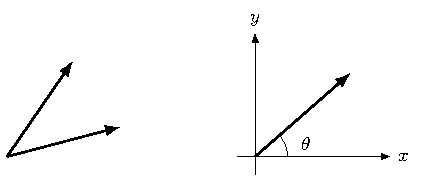
\includegraphics[width=0.75\textwidth]{figuras/angulo-entre-vectores.pdf}
        \caption{Ángulo entre dos vectores en $\R^2$.}
    \end{figure}

    Si $\beta=\{u,v\}$ es una base ordenada para $\R^2$, definimos la \textbf{orientación} de $\beta$ como el número real
    \begin{equation*}
        \mathrm{O}\begin{pmatrix}u\\v\end{pmatrix}=\frac{\det\begin{pmatrix}u\\v\end{pmatrix}}{\left|\det\begin{pmatrix}u\\v\end{pmatrix}\right|}.
    \end{equation*}
    (El denominador de esta fracción es no nulo por el Teorema~4.2.) Claramente
    \begin{equation*}
        \mathrm{O}\begin{pmatrix}u\\v\end{pmatrix}=\pm1.
    \end{equation*}
    Observe que
    \begin{equation*}
        \mathrm{O}\begin{pmatrix}e_1\\e_2\end{pmatrix}=1\qquad\text{y}\qquad\mathrm{O}\begin{pmatrix}e_1\\-e_2\end{pmatrix}=-1.
    \end{equation*}

    Recuerde que un sistema de coordenadas $\{u,v\}$ se llama de \textbf{mano derecha} si $u$ puede rotarse en dirección contraria a las manecillas del reloj a través de un ángulo $\theta$ ($0<\theta<\pi$) hasta coincidir con $v$. En caso contrario, $\{u,v\}$ se llama un sistema de \textbf{mano izquierda}. (Véase la Figura~4.2.) En general (véase el Ejercicio~12),
    \begin{equation*}
        \mathrm{O}\begin{pmatrix}u\\v\end{pmatrix}=1
    \end{equation*}
    si y solo si la base ordenada $\{u,v\}$ forma un sistema de coordenadas de mano derecha. Por conveniencia, también definimos
    \begin{equation*}
        \mathrm{O}\begin{pmatrix}u\\v\end{pmatrix}=1
    \end{equation*}
    si $\{u,v\}$ es linealmente dependiente.

    \begin{figure}[H]
        \centering
        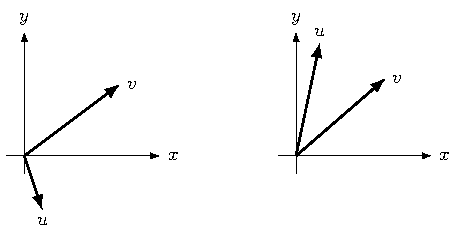
\includegraphics[width=0.85\textwidth]{figuras/sistemas-mano-derecha-izquierda.pdf}
        \caption{Un sistema de coordenadas de mano derecha (izquierda) y uno de mano izquierda (derecha).}
    \end{figure}

    Cualquier conjunto ordenado $\{u,v\}$ en $\R^2$ determina un paralelogramo de la siguiente manera. Considerando a $u$ y $v$ como flechas que emanan del origen de $\R^2$, llamamos al paralelogramo que tiene a $u$ y $v$ como lados adyacentes el \textbf{paralelogramo determinado por $u$ y $v$}. (Véase la Figura~4.3.) Observe que, si el conjunto $\{u,v\}$ es linealmente dependiente (es decir, si $u$ y $v$ son paralelos), entonces el \textquotedblleft paralelogramo\textquotedblright\ determinado por $u$ y $v$ es en realidad un segmento de recta, el cual consideramos un paralelogramo degenerado de área cero.

    \begin{figure}[H]
        \centering
        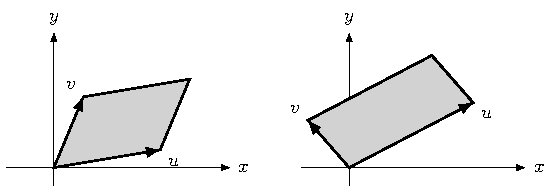
\includegraphics[width=0.85\textwidth]{figuras/paralelogramos-u-v.pdf}
        \caption{Paralelogramos determinados por $u$ y $v$.}
    \end{figure}

    Hay una relación interesante entre
    \begin{equation*}
        \mathrm{A}\begin{pmatrix}u\\v\end{pmatrix},
    \end{equation*}
    el área del paralelogramo determinado por $u$ y $v$, y
    \begin{equation*}
        \det\begin{pmatrix}u\\v\end{pmatrix},
    \end{equation*}
    la cual investigamos ahora. Observemos primero, sin embargo, que como
    \begin{equation*}
        \det\begin{pmatrix}u\\v\end{pmatrix}
    \end{equation*}
    puede ser negativo, no podemos esperar que
    \begin{equation*}
        \mathrm{A}\begin{pmatrix}u\\v\end{pmatrix}=\det\begin{pmatrix}u\\v\end{pmatrix}.
    \end{equation*}
    Pero podemos probar que
    \begin{equation*}
        \mathrm{A}\begin{pmatrix}u\\v\end{pmatrix}=\mathrm{O}\begin{pmatrix}u\\v\end{pmatrix}\cdot\det\begin{pmatrix}u\\v\end{pmatrix},
    \end{equation*}
    de donde se sigue que
    \begin{equation*}
        \mathrm{A}\begin{pmatrix}u\\v\end{pmatrix}=\left|\det\begin{pmatrix}u\\v\end{pmatrix}\right|.
    \end{equation*}

    Nuestro argumento de que
    \begin{equation*}
        \mathrm{A}\begin{pmatrix}u\\v\end{pmatrix}=\mathrm{O}\begin{pmatrix}u\\v\end{pmatrix}\cdot\det\begin{pmatrix}u\\v\end{pmatrix}
    \end{equation*}
    emplea una técnica que, aunque algo indirecta, puede generalizarse a $\R^n$. Primero, como
    \begin{equation*}
        \mathrm{O}\begin{pmatrix}u\\v\end{pmatrix}=\pm1,
    \end{equation*}
    podemos multiplicar ambos lados de la ecuación deseada por
    \begin{equation*}
        \mathrm{O}\begin{pmatrix}u\\v\end{pmatrix}
    \end{equation*}
    para obtener la forma equivalente
    \begin{equation*}
        \mathrm{O}\begin{pmatrix}u\\v\end{pmatrix}\cdot\mathrm{A}\begin{pmatrix}u\\v\end{pmatrix}=\det\begin{pmatrix}u\\v\end{pmatrix}.
    \end{equation*}
    Establecemos esta ecuación verificando que las tres condiciones del Ejercicio~11 se satisfacen para la función
    \begin{equation*}
        \delta\begin{pmatrix}u\\v\end{pmatrix}=\mathrm{O}\begin{pmatrix}u\\v\end{pmatrix}\cdot\mathrm{A}\begin{pmatrix}u\\v\end{pmatrix}.
    \end{equation*}

    (a) Comenzamos mostrando que, para cualquier número real $c$,
    \begin{equation*}
        \delta\begin{pmatrix}u\\cv\end{pmatrix}=c\cdot\delta\begin{pmatrix}u\\v\end{pmatrix}.
    \end{equation*}
    Observe que esta ecuación es válida si $c=0$, porque
    \begin{equation*}
        \delta\begin{pmatrix}u\\cv\end{pmatrix}=\mathrm{O}\begin{pmatrix}u\\0\end{pmatrix}\cdot\mathrm{A}\begin{pmatrix}u\\0\end{pmatrix}=1\cdot0=0.
    \end{equation*}
    Supongamos entonces que $c\neq0$. Considerando a $cv$ como la base del paralelogramo determinado por $u$ y $cv$, vemos que
    \begin{equation*}
        \mathrm{A}\begin{pmatrix}u\\cv\end{pmatrix}=\text{base}\times\text{altura}=|c|(\text{longitud de }v)(\text{altura})=|c|\cdot\mathrm{A}\begin{pmatrix}u\\v\end{pmatrix},
    \end{equation*}
    ya que la altura $h$ del paralelogramo determinado por $u$ y $cv$ es la misma que la del paralelogramo determinado por $u$ y $v$. (Véase la Figura~4.4.) Por tanto
    \begin{align*}
        \delta\begin{pmatrix}u\\cv\end{pmatrix}
        =\mathrm{O}\begin{pmatrix}u\\cv\end{pmatrix}\cdot\mathrm{A}\begin{pmatrix}u\\cv\end{pmatrix}
        &=\left[\frac{c}{|c|}\cdot\mathrm{O}\begin{pmatrix}u\\v\end{pmatrix}\right]\left[|c|\cdot\mathrm{A}\begin{pmatrix}u\\v\end{pmatrix}\right]\\
        &=c\cdot\mathrm{O}\begin{pmatrix}u\\v\end{pmatrix}\cdot\mathrm{A}\begin{pmatrix}u\\v\end{pmatrix}=c\cdot\delta\begin{pmatrix}u\\v\end{pmatrix}.
    \end{align*}
    Un argumento similar muestra que
    \begin{equation*}
        \delta\begin{pmatrix}cu\\v\end{pmatrix}=c\cdot\delta\begin{pmatrix}u\\v\end{pmatrix}.
    \end{equation*}

    \begin{figure}[H]
        \centering
        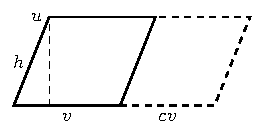
\includegraphics[width=0.5\textwidth]{figuras/paralelogramo-altura-comun.pdf}
        \caption{Los paralelogramos determinados por $u,v$ y por $u,cv$ tienen la misma altura $h$.}
    \end{figure}

    A continuación probamos que
    \begin{equation*}
        \delta\begin{pmatrix}u\\au+bw\end{pmatrix}=b\cdot\delta\begin{pmatrix}u\\w\end{pmatrix}
    \end{equation*}
    para cualesquiera $u,w\in\R^2$ y cualesquiera números reales $a$ y $b$. Como los paralelogramos determinados por $u$ y $w$, y por $u$ y $u+w$, tienen una base común $u$ y la misma altura (véase la Figura~4.5), se sigue que
    \begin{equation*}
        \mathrm{A}\begin{pmatrix}u\\w\end{pmatrix}=\mathrm{A}\begin{pmatrix}u\\u+w\end{pmatrix}.
    \end{equation*}

    \begin{figure}[H]
        \centering
        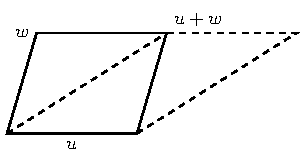
\includegraphics[width=0.55\textwidth]{figuras/paralelogramo-diagonal-suma.pdf}
        \caption{Los paralelogramos determinados por $u,w$ y por $u,u+w$ tienen base común $u$ y la misma altura.}
    \end{figure}

    Si $a=0$, entonces
    \begin{equation*}
        \delta\begin{pmatrix}u\\au+bw\end{pmatrix}=\delta\begin{pmatrix}u\\bw\end{pmatrix}=b\cdot\delta\begin{pmatrix}u\\w\end{pmatrix}
    \end{equation*}
    por el primer párrafo de (a). En caso contrario, si $a\neq0$, entonces
    \begin{equation*}
        \delta\begin{pmatrix}u\\au+bw\end{pmatrix}=a\cdot\delta\begin{pmatrix}u\\u+\dfrac{b}{a}w\end{pmatrix}=a\cdot\delta\begin{pmatrix}u\\\dfrac{b}{a}w\end{pmatrix}=b\cdot\delta\begin{pmatrix}u\\w\end{pmatrix}.
    \end{equation*}
    Así se obtiene la conclusión deseada en cualquier caso.

    Ya estamos en condiciones de mostrar que
    \begin{equation*}
        \delta\begin{pmatrix}u\\v_1+v_2\end{pmatrix}=\delta\begin{pmatrix}u\\v_1\end{pmatrix}+\delta\begin{pmatrix}u\\v_2\end{pmatrix}
    \end{equation*}
    para todos $u,v_1,v_2\in\R^2$. Como el resultado es inmediato si $u=0$, suponemos que $u\neq0$. Elijamos cualquier vector $w\in\R^2$ tal que $\{u,w\}$ sea linealmente independiente. Entonces, para cualesquiera vectores $v_1,v_2\in\R^2$, existen escalares $a_i$ y $b_i$ tales que $v_i=a_iu+b_iw$ ($i=1,2$). Así
    \begin{align*}
        \delta\begin{pmatrix}u\\v_1+v_2\end{pmatrix}
        &=\delta\begin{pmatrix}u\\(a_1+a_2)u+(b_1+b_2)w\end{pmatrix}=(b_1+b_2)\delta\begin{pmatrix}u\\w\end{pmatrix}\\
        &=\delta\begin{pmatrix}u\\a_1u+b_1w\end{pmatrix}+\delta\begin{pmatrix}u\\a_2u+b_2w\end{pmatrix}=\delta\begin{pmatrix}u\\v_1\end{pmatrix}+\delta\begin{pmatrix}u\\v_2\end{pmatrix}.
    \end{align*}
    Un argumento similar muestra que
    \begin{equation*}
        \delta\begin{pmatrix}u_1+u_2\\v\end{pmatrix}=\delta\begin{pmatrix}u_1\\v\end{pmatrix}+\delta\begin{pmatrix}u_2\\v\end{pmatrix}
    \end{equation*}
    para todos $u_1,u_2,v\in\R^2$.

    (b) Como
    \begin{equation*}
        \mathrm{A}\begin{pmatrix}u\\u\end{pmatrix}=0,\qquad\text{se sigue que}\qquad\delta\begin{pmatrix}u\\u\end{pmatrix}=\mathrm{O}\begin{pmatrix}u\\u\end{pmatrix}\cdot\mathrm{A}\begin{pmatrix}u\\u\end{pmatrix}=0
    \end{equation*}
    para cualquier $u\in\R^2$.

    (c) Como el paralelogramo determinado por $e_1$ y $e_2$ es el cuadrado unitario,
    \begin{equation*}
        \delta\begin{pmatrix}e_1\\e_2\end{pmatrix}=\mathrm{O}\begin{pmatrix}e_1\\e_2\end{pmatrix}\cdot\mathrm{A}\begin{pmatrix}e_1\\e_2\end{pmatrix}=1\cdot1=1.
    \end{equation*}

    Por tanto $\delta$ satisface las tres condiciones del Ejercicio~11, y así $\delta=\det$. Así el área del paralelogramo determinado por $u$ y $v$ es igual a
    \begin{equation*}
        \mathrm{O}\begin{pmatrix}u\\v\end{pmatrix}\cdot\det\begin{pmatrix}u\\v\end{pmatrix}.
    \end{equation*}

    Así vemos, por ejemplo, que el área del paralelogramo determinado por $u=(-1,5)$ y $v=(4,-2)$ es
    \begin{equation*}
        \left|\det\begin{pmatrix}u\\v\end{pmatrix}\right|=\left|\det\begin{pmatrix}-1&5\\4&-2\end{pmatrix}\right|=18.
    \end{equation*}

    \begin{ejercicio}
        Etiquete las siguientes afirmaciones como verdaderas o falsas.
        \begin{enumerate}[label=(\alph*)]
            \item La función $\det:M_{2\times2}(F)\to F$ es una transformación lineal.
            \item El determinante de una matriz $2\times2$ es una función lineal de cada renglón de la matriz cuando el otro renglón se mantiene fijo.
            \item Si $A\in M_{2\times2}(F)$ y $\det(A)=0$, entonces $A$ es invertible.
            \item Si $u$ y $v$ son vectores en $\R^2$ que emanan del origen, entonces el área del paralelogramo que tiene a $u$ y $v$ como lados adyacentes es
            \begin{equation*}
                \det\begin{pmatrix}u\\v\end{pmatrix}.
            \end{equation*}
            \item Un sistema de coordenadas es de mano derecha si y solo si su orientación es igual a $1$.
        \end{enumerate}
    \end{ejercicio}

    \begin{ejercicio}
        Calcule los determinantes de las siguientes matrices en $M_{2\times2}(\R)$.
        \begin{multicols}{3}
        \begin{enumerate}[label=(\alph*)]
            \item $\begin{pmatrix}6&-3\\2&4\end{pmatrix}$
            \item $\begin{pmatrix}-5&2\\6&1\end{pmatrix}$
            \item $\begin{pmatrix}8&0\\3&-1\end{pmatrix}$
        \end{enumerate}
        \end{multicols}
    \end{ejercicio}

    \begin{ejercicio}
        Calcule los determinantes de las siguientes matrices en $M_{2\times2}(\C)$.
        \begin{enumerate}[label=(\alph*)]
            \item $\begin{pmatrix}-1+i&1-4i\\3+2i&2-3i\end{pmatrix}$
            \item $\begin{pmatrix}5-2i&6+4i\\-3+i&7i\end{pmatrix}$
            \item $\begin{pmatrix}2i&3\\4&6i\end{pmatrix}$
        \end{enumerate}
    \end{ejercicio}

    \begin{ejercicio}
        Para cada uno de los siguientes pares de vectores $u$ y $v$ en $\R^2$, calcule el área del paralelogramo determinado por $u$ y $v$.
        \begin{enumerate}[label=(\alph*)]
            \item $u=(3,-2)$ y $v=(2,5)$
            \item $u=(1,3)$ y $v=(-3,1)$
            \item $u=(4,-1)$ y $v=(-6,-2)$
            \item $u=(3,4)$ y $v=(2,-6)$
        \end{enumerate}
    \end{ejercicio}

    \begin{ejercicio}
        Pruebe que, si $B$ es la matriz obtenida al intercambiar los renglones de una matriz $2\times2$ $A$, entonces $\det(B)=-\det(A)$.
    \end{ejercicio}

    \begin{ejercicio}
        Pruebe que, si las dos columnas de $A\in M_{2\times2}(F)$ son idénticas, entonces $\det(A)=0$.
    \end{ejercicio}

    \begin{ejercicio}
        Pruebe que $\det(A^t)=\det(A)$ para cualquier $A\in M_{2\times2}(F)$.
    \end{ejercicio}

    \begin{ejercicio}
        Pruebe que, si $A\in M_{2\times2}(F)$ es triangular superior, entonces $\det(A)$ es igual al producto de las entradas diagonales de $A$.
    \end{ejercicio}

    \begin{ejercicio}
        Pruebe que $\det(AB)=\det(A)\cdot\det(B)$ para cualesquiera $A,B\in M_{2\times2}(F)$.
    \end{ejercicio}

    \begin{ejercicio}
        La \textbf{adjunta clásica} de una matriz $2\times2$ $A\in M_{2\times2}(F)$ es la matriz
        \begin{equation*}
            C=\begin{pmatrix}A_{22}&-A_{12}\\-A_{21}&A_{11}\end{pmatrix}.
        \end{equation*}
        Pruebe que
        \begin{enumerate}[label=(\alph*)]
            \item $CA=AC=[\det(A)]I$.
            \item $\det(C)=\det(A)$.
            \item La adjunta clásica de $A^t$ es $C^t$.
            \item Si $A$ es invertible, entonces $A^{-1}=[\det(A)]^{-1}C$.
        \end{enumerate}
    \end{ejercicio}

    \begin{ejercicio}
        Sea $\delta:M_{2\times2}(F)\to F$ una función con las siguientes tres propiedades.
        \begin{enumerate}[label=(\roman*)]
            \item $\delta$ es una función lineal de cada renglón de la matriz cuando el otro renglón se mantiene fijo.
            \item Si los dos renglones de $A\in M_{2\times2}(F)$ son idénticos, entonces $\delta(A)=0$.
            \item Si $I$ es la matriz identidad $2\times2$, entonces $\delta(I)=1$.
        \end{enumerate}
        Pruebe que $\delta(A)=\det(A)$ para toda $A\in M_{2\times2}(F)$. (Este resultado se generaliza en la Sección~4.5.)
    \end{ejercicio}

    \begin{ejercicio}
        Sea $\{u,v\}$ una base ordenada para $\R^2$. Pruebe que
        \begin{equation*}
            \mathrm{O}\begin{pmatrix}u\\v\end{pmatrix}=1
        \end{equation*}
        si y solo si $\{u,v\}$ forma un sistema de coordenadas de mano derecha. \textit{Sugerencia:} Recuerde la definición de una rotación dada en el Ejemplo~2 de la Sección~2.1.
    \end{ejercicio}

    \section{Determinantes de orden \texorpdfstring{$n$}{n}}

    En esta sección extendemos la definición del determinante a las matrices $n\times n$ para $n\geq3$. Para esta definición, conviene introducir la siguiente notación: dada $A\in M_{n\times n}(F)$, para $n\geq2$, denotamos por $\widetilde{A}_{ij}$ la matriz $(n-1)\times(n-1)$ obtenida de $A$ al eliminar el renglón $i$ y la columna $j$. Así, para
    \begin{equation*}
        A=\begin{pmatrix}1&2&3\\4&5&6\\7&8&9\end{pmatrix}\in M_{3\times3}(\R),
    \end{equation*}
    tenemos
    \begin{equation*}
        \widetilde{A}_{11}=\begin{pmatrix}5&6\\8&9\end{pmatrix},\qquad\widetilde{A}_{13}=\begin{pmatrix}4&5\\7&8\end{pmatrix},\qquad\text{y}\qquad\widetilde{A}_{32}=\begin{pmatrix}1&3\\4&6\end{pmatrix},
    \end{equation*}
    y para
    \begin{equation*}
        B=\begin{pmatrix}1&-1&2&-1\\-3&4&1&-1\\2&-5&-3&8\\-2&6&-4&1\end{pmatrix}\in M_{4\times4}(\R),
    \end{equation*}
    tenemos
    \begin{equation*}
        \widetilde{B}_{23}=\begin{pmatrix}1&-1&-1\\2&-5&8\\-2&6&1\end{pmatrix}\qquad\text{y}\qquad\widetilde{B}_{42}=\begin{pmatrix}1&2&-1\\-3&1&-1\\2&-3&8\end{pmatrix}.
    \end{equation*}

    \begin{definicion}[Determinante]
        Sea $A\in M_{n\times n}(F)$. Si $n=1$, de modo que $A=(A_{11})$, definimos $\det(A)=A_{11}$. Para $n\geq2$, definimos $\det(A)$ recursivamente como
        \begin{equation*}
            \det(A)=\sum_{j=1}^n(-1)^{1+j}A_{1j}\cdot\det(\widetilde{A}_{1j}).
        \end{equation*}
    \end{definicion}

    El escalar $\det(A)$ se llama el \textbf{determinante} de $A$ y también se denota $|A|$. El escalar
    \begin{equation*}
        (-1)^{i+j}\det(\widetilde{A}_{ij})
    \end{equation*}
    se llama el \textbf{cofactor} de la entrada de $A$ en el renglón $i$, columna $j$.

    Denotando
    \begin{equation*}
        c_{ij}=(-1)^{i+j}\det(\widetilde{A}_{ij})
    \end{equation*}
    el cofactor de la entrada del renglón $i$, columna $j$ de $A$, podemos expresar la fórmula del determinante de $A$ como
    \begin{equation*}
        \det(A)=A_{11}c_{11}+A_{12}c_{12}+\cdots+A_{1n}c_{1n}.
    \end{equation*}
    Así el determinante de $A$ es igual a la suma de los productos de cada entrada del renglón $1$ de $A$ por su cofactor. Esta fórmula se llama \textbf{expansión por cofactores a lo largo del primer renglón}. Observe que, para matrices $2\times2$, esta definición del determinante coincide con la dada en la Sección~4.1 porque
    \begin{equation*}
        \det(A)=A_{11}(-1)^{1+1}\det(\widetilde{A}_{11})+A_{12}(-1)^{1+2}\det(\widetilde{A}_{12})=A_{11}A_{22}-A_{12}A_{21}.
    \end{equation*}

    \begin{ejemplo}
        Sea
        \begin{equation*}
            A=\begin{pmatrix}1&3&-3\\-3&-5&2\\-4&4&-6\end{pmatrix}\in M_{3\times3}(\R).
        \end{equation*}
        Usando expansión por cofactores a lo largo del primer renglón de $A$, obtenemos
        \begin{align*}
            \det(A)&=(-1)^{1+1}A_{11}\cdot\det(\widetilde{A}_{11})+(-1)^{1+2}A_{12}\cdot\det(\widetilde{A}_{12})+(-1)^{1+3}A_{13}\cdot\det(\widetilde{A}_{13})\\
            &=(-1)^2(1)\cdot\det\begin{pmatrix}-5&2\\4&-6\end{pmatrix}+(-1)^3(3)\cdot\det\begin{pmatrix}-3&2\\-4&-6\end{pmatrix}\\
            &\qquad{}+(-1)^4(-3)\cdot\det\begin{pmatrix}-3&-5\\-4&4\end{pmatrix}\\
            &=1\big[-5(-6)-2(4)\big]-3\big[-3(-6)-2(-4)\big]-3\big[-3(4)-(-5)(-4)\big]\\
            &=1(22)-3(26)-3(-32)\\
            &=40.
        \end{align*}
    \end{ejemplo}

    \begin{ejemplo}
        Sea
        \begin{equation*}
            B=\begin{pmatrix}0&1&3\\-2&-3&-5\\4&-4&4\end{pmatrix}\in M_{3\times3}(\R).
        \end{equation*}
        Usando expansión por cofactores a lo largo del primer renglón de $B$, obtenemos
        \begin{align*}
            \det(B)&=(-1)^{1+1}B_{11}\cdot\det(\widetilde{B}_{11})+(-1)^{1+2}B_{12}\cdot\det(\widetilde{B}_{12})+(-1)^{1+3}B_{13}\cdot\det(\widetilde{B}_{13})\\
            &=(-1)^2(0)\cdot\det\begin{pmatrix}-3&-5\\-4&4\end{pmatrix}+(-1)^3(1)\cdot\det\begin{pmatrix}-2&-5\\4&4\end{pmatrix}\\
            &\qquad{}+(-1)^4(3)\cdot\det\begin{pmatrix}-2&-3\\4&-4\end{pmatrix}\\
            &=0-1\big[-2(4)-(-5)(4)\big]+3\big[-2(-4)-(-3)(4)\big]\\
            &=0-1(12)+3(20)\\
            &=48.
        \end{align*}
    \end{ejemplo}

    \begin{ejemplo}
        Sea
        \begin{equation*}
            C=\begin{pmatrix}2&0&0&1\\0&1&3&-3\\-2&-3&-5&2\\4&-4&4&-6\end{pmatrix}\in M_{4\times4}(\R).
        \end{equation*}
        Usando expansión por cofactores a lo largo del primer renglón de $C$ y los resultados de los Ejemplos~1 y~2, obtenemos
        \begin{align*}
            \det(C)&=(-1)^2(2)\cdot\det(\widetilde{C}_{11})+(-1)^3(0)\cdot\det(\widetilde{C}_{12})+(-1)^4(0)\cdot\det(\widetilde{C}_{13})+(-1)^5(1)\cdot\det(\widetilde{C}_{14})\\
            &=(-1)^2(2)\cdot\det\begin{pmatrix}1&3&-3\\-3&-5&2\\-4&4&-6\end{pmatrix}+0+0+(-1)^5(1)\cdot\det\begin{pmatrix}0&1&3\\-2&-3&-5\\4&-4&4\end{pmatrix}\\
            &=2(40)+0+0-1(48)\\
            &=32.
        \end{align*}
    \end{ejemplo}

    \begin{ejemplo}
        El determinante de la matriz identidad $n\times n$ es $1$. Probamos esta afirmación por inducción matemática sobre $n$. El resultado es claramente cierto para la matriz identidad $1\times1$. Supongamos que el determinante de la matriz identidad $(n-1)\times(n-1)$ es $1$ para algún $n\geq2$, y sea $I$ la matriz identidad $n\times n$. Usando expansión por cofactores a lo largo del primer renglón de $I$, obtenemos
        \begin{align*}
            \det(I)&=(-1)^2(1)\cdot\det(\widetilde{I}_{11})+(-1)^3(0)\cdot\det(\widetilde{I}_{12})+\cdots+(-1)^{1+n}(0)\cdot\det(\widetilde{I}_{1n})\\
            &=1(1)+0+\cdots+0\\
            &=1,
        \end{align*}
        porque $\widetilde{I}_{11}$ es la matriz identidad $(n-1)\times(n-1)$. Esto muestra que el determinante de la matriz identidad $n\times n$ es $1$, y así el determinante de cualquier matriz identidad es $1$ por el principio de inducción matemática.
    \end{ejemplo}

    Como se ilustra en el Ejemplo~4, el cálculo de un determinante usando la definición recursiva es extremadamente tedioso, incluso para matrices tan pequeñas como $4\times4$. Más adelante en esta sección presentamos un método más eficiente para evaluar determinantes, pero primero debemos aprender más sobre ellos.

    Recuerde del Teorema~4.1 (p.~200) que, aunque el determinante de una matriz $2\times2$ \textit{no} es una transformación lineal, sí es una función lineal de cada renglón cuando el otro renglón se mantiene fijo. Mostramos ahora que una propiedad similar es cierta para determinantes de cualquier tamaño.

    \begin{teorema}
        El determinante de una matriz $n\times n$ es una función lineal de cada renglón cuando los demás renglones se mantienen fijos. Es decir, para $1\leq r\leq n$, tenemos
        \begin{equation*}
            \det\begin{pmatrix}a_1\\\vdots\\a_{r-1}\\u+kv\\a_{r+1}\\\vdots\\a_n\end{pmatrix}
            =\det\begin{pmatrix}a_1\\\vdots\\a_{r-1}\\u\\a_{r+1}\\\vdots\\a_n\end{pmatrix}
            +k\det\begin{pmatrix}a_1\\\vdots\\a_{r-1}\\v\\a_{r+1}\\\vdots\\a_n\end{pmatrix}
        \end{equation*}
        siempre que $k$ sea un escalar y $u$, $v$, y cada $a_i$ sean vectores renglón en $F^n$.
    \end{teorema}
    \begin{proof}
        La demostración es por inducción matemática sobre $n$. El resultado es inmediato si $n=1$. Supongamos que, para algún entero $n\geq2$, el determinante de cualquier matriz $(n-1)\times(n-1)$ es una función lineal de cada renglón cuando los demás renglones se mantienen fijos. Sea $A$ una matriz $n\times n$ con renglones $a_1,a_2,\dots,a_n$, respectivamente, y supongamos que, para algún $r$ ($1\leq r\leq n$), tenemos $a_r=u+kv$ para algunos $u,v\in F^n$ y algún escalar $k$. Sean $u=(b_1,b_2,\dots,b_n)$ y $v=(c_1,c_2,\dots,c_n)$, y sean $B$ y $C$ las matrices obtenidas de $A$ al reemplazar el renglón $r$ de $A$ por $u$ y $v$, respectivamente. Dejamos al lector la demostración de este hecho para el caso $r=1$. Para $r>1$ y $1\leq j\leq n$, los renglones de $\widetilde{A}_{1j}$, $\widetilde{B}_{1j}$, y $\widetilde{C}_{1j}$ son iguales excepto por el renglón $r-1$. Más aún, el renglón $r-1$ de $\widetilde{A}_{1j}$ es
        \begin{equation*}
            (b_1+kc_1,\dots,b_{j-1}+kc_{j-1},b_{j+1}+kc_{j+1},\dots,b_n+kc_n),
        \end{equation*}
        el cual es la suma del renglón $r-1$ de $\widetilde{B}_{1j}$ y $k$ veces el renglón $r-1$ de $\widetilde{C}_{1j}$. Como $\widetilde{B}_{1j}$ y $\widetilde{C}_{1j}$ son matrices $(n-1)\times(n-1)$, tenemos
        \begin{equation*}
            \det(\widetilde{A}_{1j})=\det(\widetilde{B}_{1j})+k\det(\widetilde{C}_{1j})
        \end{equation*}
        por la hipótesis de inducción. Así, como $A_{1j}=B_{1j}=C_{1j}$, tenemos
        \begin{align*}
            \det(A)&=\sum_{j=1}^n(-1)^{1+j}A_{1j}\cdot\det(\widetilde{A}_{1j})\\
            &=\sum_{j=1}^n(-1)^{1+j}A_{1j}\cdot\Big[\det(\widetilde{B}_{1j})+k\det(\widetilde{C}_{1j})\Big]\\
            &=\sum_{j=1}^n(-1)^{1+j}A_{1j}\cdot\det(\widetilde{B}_{1j})+k\sum_{j=1}^n(-1)^{1+j}A_{1j}\cdot\det(\widetilde{C}_{1j})\\
            &=\det(B)+k\det(C).
        \end{align*}
        Esto muestra que el teorema es cierto para matrices $n\times n$, y así el teorema es cierto para todas las matrices cuadradas por inducción matemática.
    \end{proof}

    \begin{corolario}
        Si $A\in M_{n\times n}(F)$ tiene un renglón formado enteramente por ceros, entonces $\det(A)=0$.
    \end{corolario}
    \begin{proof}
        Supongamos que el renglón $r$ de $A$ es el vector cero $0\in F^n$. Como $0=0+1\cdot0$, el Teorema~4.3 aplicado dos veces al renglón $r$ (con $u=v=0$ y $k=1$) da
        \begin{equation*}
            \det(A)=\det(A)+1\cdot\det(A)=2\det(A),
        \end{equation*}
        donde ambos determinantes del lado derecho corresponden a matrices con el renglón $r$ igual a $0$, es decir, iguales a $A$. Por tanto $\det(A)=2\det(A)$, de donde $\det(A)=0$.
    \end{proof}

    La definición de un determinante requiere que el determinante de una matriz se evalúe mediante expansión por cofactores a lo largo del primer renglón. Nuestro siguiente teorema muestra que el determinante de una matriz cuadrada puede evaluarse mediante expansión por cofactores a lo largo de \textit{cualquier} renglón. Su demostración requiere el siguiente resultado técnico.

    \begin{lema}
        Sea $B\in M_{n\times n}(F)$, donde $n\geq2$. Si el renglón $i$ de $B$ es igual a $e_k$ para algún $k$ ($1\leq k\leq n$), entonces $\det(B)=(-1)^{i+k}\det(\widetilde{B}_{ik})$.
    \end{lema}
    \begin{proof}
        La demostración es por inducción matemática sobre $n$. El lema se prueba fácilmente para $n=2$. Supongamos que, para algún entero $n\geq3$, el lema es cierto para matrices $(n-1)\times(n-1)$, y sea $B$ una matriz $n\times n$ en la que el renglón $i$ de $B$ es igual a $e_k$ para algún $k$ ($1\leq k\leq n$). El resultado se sigue de inmediato de la definición del determinante si $i=1$. Supongamos entonces que $1<i\leq n$. Para cada $j\neq k$ ($1\leq j\leq n$), sea $C_{ij}$ la matriz $(n-2)\times(n-2)$ obtenida de $B$ al eliminar los renglones $1$ e $i$ y las columnas $j$ y $k$. Para cada $j$, el renglón $i-1$ de $\widetilde{B}_{1j}$ es el siguiente vector en $F^{n-1}$:
        \begin{equation*}
            \begin{cases}
                e_{k-1}&\text{si }j<k\\
                0&\text{si }j=k\\
                e_k&\text{si }j>k.
            \end{cases}
        \end{equation*}
        Por tanto, por la hipótesis de inducción y el corolario al Teorema~4.3, tenemos
        \begin{equation*}
            \det(\widetilde{B}_{1j})=
            \begin{cases}
                (-1)^{(i-1)+(k-1)}\det(C_{ij})&\text{si }j<k\\
                0&\text{si }j=k\\
                (-1)^{(i-1)+k}\det(C_{ij})&\text{si }j>k.
            \end{cases}
        \end{equation*}
        Por tanto
        \begin{align*}
            \det(B)&=\sum_{j=1}^n(-1)^{1+j}B_{1j}\cdot\det(\widetilde{B}_{1j})\\
            &=\sum_{j<k}(-1)^{1+j}B_{1j}\cdot\det(\widetilde{B}_{1j})+\sum_{j>k}(-1)^{1+j}B_{1j}\cdot\det(\widetilde{B}_{1j})\\
            &=\sum_{j<k}(-1)^{1+j}B_{1j}\cdot\Big[(-1)^{(i-1)+(k-1)}\det(C_{ij})\Big]\\
            &\qquad{}+\sum_{j>k}(-1)^{1+j}B_{1j}\cdot\Big[(-1)^{(i-1)+k}\det(C_{ij})\Big]\\
            &=(-1)^{i+k}\left[\sum_{j<k}(-1)^{1+j}B_{1j}\cdot\det(C_{ij})+\sum_{j>k}(-1)^{1+(j-1)}B_{1j}\cdot\det(C_{ij})\right].
        \end{align*}
        Como la expresión dentro del corchete anterior es la expansión por cofactores de $\widetilde{B}_{ik}$ a lo largo del primer renglón, se sigue que
        \begin{equation*}
            \det(B)=(-1)^{i+k}\det(\widetilde{B}_{ik}).
        \end{equation*}
        Esto muestra que el lema es cierto para matrices $n\times n$, y así el lema es cierto para todas las matrices cuadradas por inducción matemática.
    \end{proof}

    Estamos ahora en condiciones de probar que la expansión por cofactores a lo largo de cualquier renglón puede usarse para evaluar el determinante de una matriz cuadrada.

    \begin{teorema}
        El determinante de una matriz cuadrada puede evaluarse mediante expansión por cofactores a lo largo de cualquier renglón. Es decir, si $A\in M_{n\times n}(F)$, entonces, para cualquier entero $i$ ($1\leq i\leq n$),
        \begin{equation*}
            \det(A)=\sum_{j=1}^n(-1)^{i+j}A_{ij}\cdot\det(\widetilde{A}_{ij}).
        \end{equation*}
    \end{teorema}
    \begin{proof}
        La expansión por cofactores a lo largo del primer renglón de $A$ da el determinante de $A$ por definición. Así el resultado es cierto si $i=1$. Fijemos $i>1$. El renglón $i$ de $A$ puede escribirse como $\sum_{j=1}^nA_{ij}e_j$. Para $1\leq j\leq n$, denotemos por $B_j$ la matriz obtenida de $A$ al reemplazar el renglón $i$ de $A$ por $e_j$. Entonces, por el Teorema~4.3 y el lema anterior, tenemos
        \begin{equation*}
            \det(A)=\sum_{j=1}^nA_{ij}\det(B_j)=\sum_{j=1}^n(-1)^{i+j}A_{ij}\cdot\det(\widetilde{A}_{ij}).\qedhere
        \end{equation*}
    \end{proof}

    \begin{corolario}
        Si $A\in M_{n\times n}(F)$ tiene dos renglones idénticos, entonces $\det(A)=0$.
    \end{corolario}
    \begin{proof}
        La demostración es por inducción matemática sobre $n$. Dejamos al lector la demostración del resultado en el caso $n=2$. Supongamos que, para algún entero $n\geq3$, esto es cierto para matrices $(n-1)\times(n-1)$, y sean los renglones $r$ y $s$ de $A\in M_{n\times n}(F)$ idénticos para $r\neq s$. Como $n\geq3$, podemos elegir un entero $i$ ($1\leq i\leq n$) distinto de $r$ y $s$. Ahora bien,
        \begin{equation*}
            \det(A)=\sum_{j=1}^n(-1)^{i+j}A_{ij}\cdot\det(\widetilde{A}_{ij})
        \end{equation*}
        por el Teorema~4.4. Como cada $\widetilde{A}_{ij}$ es una matriz $(n-1)\times(n-1)$ con dos renglones idénticos, la hipótesis de inducción implica que cada $\det(\widetilde{A}_{ij})=0$, y por tanto $\det(A)=0$. Esto completa la demostración para matrices $n\times n$, y así el resultado es cierto para todas las matrices cuadradas por inducción matemática.
    \end{proof}

    Es posible evaluar determinantes de manera más eficiente combinando la expansión por cofactores con el uso de operaciones elementales de renglón. Antes de desarrollar tal proceso, necesitamos aprender qué le sucede al determinante de una matriz si se realiza sobre ella una operación elemental de renglón. El Teorema~4.3 proporciona esta información para las operaciones elementales de renglón de tipo 2 (aquellas en las que un renglón se multiplica por un escalar no nulo). A continuación dirigimos nuestra atención a las operaciones elementales de renglón de tipo 1 (aquellas en las que se intercambian dos renglones).

    \begin{teorema}
        Si $A\in M_{n\times n}(F)$ y $B$ es una matriz obtenida de $A$ al intercambiar cualesquiera dos renglones de $A$, entonces $\det(B)=-\det(A)$.
    \end{teorema}
    \begin{proof}
        Sean los renglones de $A\in M_{n\times n}(F)$ $a_1,a_2,\dots,a_n$, y sea $B$ la matriz obtenida de $A$ al intercambiar los renglones $r$ y $s$, donde $r<s$. Así
        \begin{equation*}
            A=\begin{pmatrix}a_1\\\vdots\\a_r\\\vdots\\a_s\\\vdots\\a_n\end{pmatrix}\qquad\text{y}\qquad B=\begin{pmatrix}a_1\\\vdots\\a_s\\\vdots\\a_r\\\vdots\\a_n\end{pmatrix}.
        \end{equation*}
        Consideremos la matriz obtenida de $A$ al reemplazar los renglones $r$ y $s$ por $a_r+a_s$. Por el corolario al Teorema~4.4 y el Teorema~4.3, tenemos
        \begin{align*}
            0&=\det\begin{pmatrix}a_1\\\vdots\\a_r+a_s\\\vdots\\a_r+a_s\\\vdots\\a_n\end{pmatrix}
            =\det\begin{pmatrix}a_1\\\vdots\\a_r\\\vdots\\a_r+a_s\\\vdots\\a_n\end{pmatrix}
            +\det\begin{pmatrix}a_1\\\vdots\\a_s\\\vdots\\a_r+a_s\\\vdots\\a_n\end{pmatrix}\\
            &=\det\begin{pmatrix}a_1\\\vdots\\a_r\\\vdots\\a_r\\\vdots\\a_n\end{pmatrix}
            +\det\begin{pmatrix}a_1\\\vdots\\a_r\\\vdots\\a_s\\\vdots\\a_n\end{pmatrix}
            +\det\begin{pmatrix}a_1\\\vdots\\a_s\\\vdots\\a_r\\\vdots\\a_n\end{pmatrix}
            +\det\begin{pmatrix}a_1\\\vdots\\a_s\\\vdots\\a_s\\\vdots\\a_n\end{pmatrix}\\
            &=0+\det(A)+\det(B)+0.
        \end{align*}
        Por tanto $\det(B)=-\det(A)$.
    \end{proof}

    Completamos ahora nuestra investigación de cómo una operación elemental de renglón afecta al determinante de una matriz, mostrando que las operaciones elementales de renglón de tipo 3 no cambian el determinante de una matriz.

    \begin{teorema}
        Sea $A\in M_{n\times n}(F)$, y sea $B$ una matriz obtenida al sumar un múltiplo de un renglón de $A$ a otro renglón de $A$. Entonces $\det(B)=\det(A)$.
    \end{teorema}
    \begin{proof}
        Supongamos que $B$ es la matriz $n\times n$ obtenida al sumar $k$ veces el renglón $r$ al renglón $s$, donde $r\neq s$. Sean los renglones de $A$ $a_1,a_2,\dots,a_n$, y sean los renglones de $B$ $b_1,b_2,\dots,b_n$. Entonces $b_i=a_i$ para $i\neq s$, y $b_s=a_s+ka_r$. Sea $C$ la matriz obtenida de $A$ al reemplazar el renglón $s$ con $a_r$. Aplicando el Teorema~4.3 al renglón $s$ de $B$, obtenemos
        \begin{equation*}
            \det(B)=\det(A)+k\det(C)=\det(A)
        \end{equation*}
        porque $\det(C)=0$ por el corolario al Teorema~4.4.
    \end{proof}

    En el Teorema~4.2 (p.~201) probamos que una matriz $2\times2$ es invertible si y solo si su determinante es no nulo. Como consecuencia del Teorema~4.6, podemos probar la mitad prometida de la generalización de este resultado en el siguiente corolario. El recíproco se prueba en el corolario al Teorema~4.7.

    \begin{corolario}
        Si $A\in M_{n\times n}(F)$ tiene rango menor que $n$, entonces $\det(A)=0$.
    \end{corolario}
    \begin{proof}
        Si el rango de $A$ es menor que $n$, entonces los renglones $a_1,a_2,\dots,a_n$ de $A$ son linealmente dependientes por el Ejercicio~91 de la Sección~1.5. Así algún renglón de $A$, digamos el renglón $r$, es una combinación lineal de los demás renglones. Por tanto existen escalares $c_i$ tales que
        \begin{equation*}
            a_r=c_1a_1+\cdots+c_{r-1}a_{r-1}+c_{r+1}a_{r+1}+\cdots+c_na_n.
        \end{equation*}
        Sea $B$ la matriz obtenida de $A$ al sumar $-c_i$ veces el renglón $i$ al renglón $r$ para cada $i\neq r$. Entonces el renglón $r$ de $B$ está formado enteramente por ceros, y así $\det(B)=0$. Pero por el Teorema~4.6, $\det(B)=\det(A)$. Por tanto $\det(A)=0$.
    \end{proof}

    Las siguientes reglas resumen el efecto de una operación elemental de renglón sobre el determinante de una matriz $A\in M_{n\times n}(F)$.
    \begin{enumerate}[label=(\alph*)]
        \item Si $B$ es una matriz obtenida al intercambiar cualesquiera dos renglones de $A$, entonces $\det(B)=-\det(A)$.
        \item Si $B$ es una matriz obtenida al multiplicar un renglón de $A$ por un escalar no nulo $k$, entonces $\det(B)=k\det(A)$.
        \item Si $B$ es una matriz obtenida al sumar un múltiplo de un renglón de $A$ a otro renglón, entonces $\det(B)=\det(A)$.
    \end{enumerate}

    Estos hechos pueden usarse para simplificar la evaluación de determinantes. Consideremos, por ejemplo, la matriz del Ejemplo~2:
    \begin{equation*}
        A=\begin{pmatrix}1&3&-3\\-3&-5&2\\-4&4&-6\end{pmatrix}.
    \end{equation*}
    Sumando $3$ veces el renglón 1 de $A$ al renglón 2 y $4$ veces el renglón 1 al renglón 3, obtenemos
    \begin{equation*}
        M=\begin{pmatrix}1&4&-3\\0&4&-7\\0&16&-18\end{pmatrix}.
    \end{equation*}
    Como $M$ se obtuvo al realizar dos operaciones elementales de renglón de tipo 3 sobre $A$, tenemos $\det(A)=\det(M)$. La expansión por cofactores de $M$ a lo largo del primer renglón da
    \begin{align*}
        \det(M)&=(-1)^{1+1}(1)\cdot\det(\widetilde{M}_{11})+(-1)^{1+2}(4)\cdot\det(\widetilde{M}_{12})+(-1)^{1+3}(-3)\cdot\det(\widetilde{M}_{13}).
    \end{align*}
    Tanto $\widetilde{M}_{12}$ como $\widetilde{M}_{13}$ tienen una columna formada enteramente por ceros, y así $\det(\widetilde{M}_{12})=\det(\widetilde{M}_{13})=0$ por el corolario al Teorema~4.6 (aplicado a las columnas, como se justifica en la Sección~4.3). Por tanto
    \begin{align*}
        \det(M)&=(-1)^{1+1}(1)\cdot\det(\widetilde{M}_{11})=(-1)^{1+1}(1)\cdot\det\begin{pmatrix}4&-7\\16&-18\end{pmatrix}\\
        &=1\big[4(-18)-(-7)(16)\big]=1(40)=40.
    \end{align*}
    Así, con el uso de dos operaciones elementales de renglón de tipo 3, hemos reducido el cálculo de $\det(A)$ a la evaluación de un determinante de una matriz $2\times2$.

    Pero podemos hacer aún mejor. Si sumamos $-4$ veces el renglón 2 de $M$ al renglón 3 (otra operación elemental de renglón de tipo 3), obtenemos
    \begin{equation*}
        P=\begin{pmatrix}1&4&-3\\0&4&-7\\0&0&10\end{pmatrix}.
    \end{equation*}
    Evaluando $\det(P)$ mediante expansión por cofactores a lo largo del primer renglón, tenemos
    \begin{equation*}
        \det(P)=(-1)^{1+1}(1)\cdot\det(\widetilde{P}_{11})=(-1)^{1+1}(1)\cdot\det\begin{pmatrix}4&-7\\0&10\end{pmatrix}=1\cdot4\cdot10=40,
    \end{equation*}
    como se describió antes. Como $\det(A)=\det(M)=\det(P)$, se sigue que $\det(A)=40$.

    El cálculo precedente de $\det(P)$ ilustra un hecho general importante. \textit{El determinante de una matriz triangular superior es el producto de sus entradas diagonales.} (Véase el Ejercicio~35.) Usando operaciones elementales de renglón de tipos 1 y 3 únicamente, podemos transformar cualquier matriz cuadrada en una matriz triangular superior, y así podemos evaluar fácilmente el determinante de cualquier matriz cuadrada. Los siguientes dos ejemplos ilustran esta técnica.

    \begin{ejemplo}
        Para evaluar el determinante de la matriz
        \begin{equation*}
            B=\begin{pmatrix}0&1&3\\-2&-3&-5\\4&-4&4\end{pmatrix}
        \end{equation*}
        del Ejemplo~3, debemos comenzar con un intercambio de renglones. Intercambiando los renglones 1 y 2 de $B$ se produce
        \begin{equation*}
            C=\begin{pmatrix}-2&-3&-5\\0&1&3\\4&-4&4\end{pmatrix}.
        \end{equation*}
        Mediante una sucesión de operaciones elementales de renglón de tipo 3, podemos transformar $C$ en una matriz triangular superior:
        \begin{equation*}
            \begin{pmatrix}-2&-3&-5\\0&1&3\\4&-4&4\end{pmatrix}
            \longrightarrow
            \begin{pmatrix}-2&-3&-5\\0&1&3\\0&-10&-6\end{pmatrix}
            \longrightarrow
            \begin{pmatrix}-2&-3&-5\\0&1&3\\0&0&24\end{pmatrix}.
        \end{equation*}
        Así $\det(C)=-2\cdot1\cdot24=-48$. Como $C$ se obtuvo de $B$ mediante un intercambio de renglones, se sigue que
        \begin{equation*}
            \det(B)=-\det(C)=48.
        \end{equation*}
    \end{ejemplo}

    \begin{ejemplo}
        La técnica del Ejemplo~6 puede usarse para evaluar el determinante de la matriz
        \begin{equation*}
            C=\begin{pmatrix}2&0&0&1\\0&1&3&-3\\-2&-3&-5&2\\4&-4&4&-6\end{pmatrix}
        \end{equation*}
        del Ejemplo~4. Esta matriz puede transformarse en una matriz triangular superior mediante la siguiente sucesión de operaciones elementales de renglón de tipo 3:
        \begin{equation*}
            \begin{pmatrix}2&0&0&1\\0&1&3&-3\\-2&-3&-5&2\\4&-4&4&-6\end{pmatrix}
            \longrightarrow
            \begin{pmatrix}2&0&0&1\\0&1&3&-3\\0&-3&-5&3\\0&-4&4&-8\end{pmatrix}
            \longrightarrow
            \begin{pmatrix}2&0&0&1\\0&1&3&-3\\0&0&4&-6\\0&0&16&-20\end{pmatrix}
        \end{equation*}
        \begin{equation*}
            \longrightarrow
            \begin{pmatrix}2&0&0&1\\0&1&3&-3\\0&0&4&-6\\0&0&0&4\end{pmatrix}.
        \end{equation*}
        Así $\det(C)=2\cdot1\cdot4\cdot4=32$.
    \end{ejemplo}

    El uso de operaciones elementales de renglón para evaluar determinantes, como se ilustra en el Ejemplo~7, es mucho más eficiente que el uso de la expansión por cofactores. Consideremos primero la evaluación de una matriz $2\times2$. Como
    \begin{equation*}
        \det\begin{pmatrix}a&b\\c&d\end{pmatrix}=ad-bc,
    \end{equation*}
    la evaluación del determinante de una matriz $2\times2$ requiere $2$ multiplicaciones (y $1$ resta). Para $n\geq3$, evaluar el determinante de una matriz $n\times n$ mediante expansión por cofactores a lo largo de cualquier renglón expresa el determinante como una suma de $n$ productos que involucran determinantes de matrices $(n-1)\times(n-1)$. En total, la evaluación del determinante de una matriz $n\times n$ mediante expansión por cofactores a lo largo de cualquier renglón requiere más de $n!$ multiplicaciones, mientras que evaluar el determinante de una matriz $n\times n$ mediante operaciones elementales de renglón, como en los Ejemplos~5 y~6, puede mostrarse que requiere solo $(n^3+2n-3)/3$ multiplicaciones. Para evaluar el determinante de una matriz $20\times20$, la cual no es grande según los estándares actuales, la expansión por cofactores a lo largo de un renglón requiere más de $20!\approx2.4\times10^{18}$ multiplicaciones. Así una computadora que realizara mil millones de multiplicaciones por segundo tardaría más de $77$ años en evaluar el determinante de una matriz $20\times20$ mediante este método. En cambio, el método que usa operaciones elementales de renglón requiere solo $2679$ multiplicaciones para este cálculo, ¡lo cual tomaría a la misma computadora menos de tres millonésimas de segundo! Es fácil ver por qué la mayoría de los programas de computadora para evaluar el determinante de una matriz arbitraria no usan expansión por cofactores.

    En esta sección, definimos el determinante de una matriz cuadrada en términos de expansión por cofactores a lo largo del primer renglón. Después mostramos que el determinante de una matriz cuadrada puede evaluarse usando expansión por cofactores a lo largo de \textit{cualquier} renglón. Además, mostramos que el determinante posee varias propiedades especiales, incluyendo propiedades que nos permiten calcular $\det(B)$ a partir de $\det(A)$ siempre que $B$ sea una matriz obtenida de $A$ mediante una operación elemental de renglón. Estas propiedades nos permiten evaluar determinantes de manera mucho más eficiente. En la siguiente sección, continuamos con este enfoque para descubrir propiedades adicionales de los determinantes.

    \begin{ejercicio}
        Etiquete las siguientes afirmaciones como verdaderas o falsas.
        \begin{enumerate}[label=(\alph*)]
            \item La función $\det:M_{n\times n}(F)\to F$ es una transformación lineal.
            \item El determinante de una matriz cuadrada puede evaluarse mediante expansión por cofactores a lo largo de cualquier renglón.
            \item Si dos renglones de una matriz cuadrada $A$ son idénticos, entonces $\det(A)=0$.
            \item Si $B$ es una matriz obtenida de una matriz cuadrada $A$ al intercambiar dos renglones cualesquiera, entonces $\det(B)=-\det(A)$.
            \item Si $B$ es una matriz obtenida de una matriz cuadrada $A$ al multiplicar un renglón de $A$ por un escalar, entonces $\det(B)=\det(A)$.
            \item Si $B$ es una matriz obtenida de una matriz cuadrada $A$ al sumar $k$ veces el renglón $i$ al renglón $j$, entonces $\det(B)=k\det(A)$.
            \item Si $A\in M_{n\times n}(F)$ tiene rango $n$, entonces $\det(A)=0$.
            \item El determinante de una matriz triangular superior es igual al producto de sus entradas diagonales.
        \end{enumerate}
    \end{ejercicio}

    \begin{ejercicio}
        Halle el valor de $k$ que satisface la siguiente ecuación:
        \begin{equation*}
            \det\begin{pmatrix}3a_1&3a_2&3a_3\\3b_1&3b_2&3b_3\\3c_1&3c_2&3c_3\end{pmatrix}=k\det\begin{pmatrix}a_1&a_2&a_3\\b_1&b_2&b_3\\c_1&c_2&c_3\end{pmatrix}.
        \end{equation*}
    \end{ejercicio}

    \begin{ejercicio}
        Halle el valor de $k$ que satisface la siguiente ecuación:
        \begin{equation*}
            \det\begin{pmatrix}2a_1&2a_2&2a_3\\3b_1+5c_1&3b_2+5c_2&3b_3+5c_3\\7c_1&7c_2&7c_3\end{pmatrix}=k\det\begin{pmatrix}a_1&a_2&a_3\\b_1&b_2&b_3\\c_1&c_2&c_3\end{pmatrix}.
        \end{equation*}
    \end{ejercicio}

    \begin{ejercicio}
        Halle el valor de $k$ que satisface la siguiente ecuación:
        \begin{equation*}
            \det\begin{pmatrix}b_1+c_1&b_2+c_2&b_3+c_3\\a_1+c_1&a_2+c_2&a_3+c_3\\a_1+b_1&a_2+b_2&a_3+b_3\end{pmatrix}=k\det\begin{pmatrix}a_1&a_2&a_3\\b_1&b_2&b_3\\c_1&c_2&c_3\end{pmatrix}.
        \end{equation*}
    \end{ejercicio}

    En los Ejercicios~5 al~12, evalúe el determinante de la matriz dada mediante expansión por cofactores a lo largo del renglón indicado.

    \begin{ejercicio}
        $\begin{pmatrix}0&1&2\\-1&0&-3\\2&3&0\end{pmatrix}$ a lo largo del primer renglón
    \end{ejercicio}

    \begin{ejercicio}
        $\begin{pmatrix}1&0&2\\0&1&5\\-1&3&0\end{pmatrix}$ a lo largo del primer renglón
    \end{ejercicio}

    \begin{ejercicio}
        $\begin{pmatrix}0&1&2\\-1&0&-3\\2&3&0\end{pmatrix}$ a lo largo del segundo renglón
    \end{ejercicio}

    \begin{ejercicio}
        $\begin{pmatrix}1&0&2\\0&1&5\\-1&3&0\end{pmatrix}$ a lo largo del tercer renglón
    \end{ejercicio}

    \begin{ejercicio}
        $\begin{pmatrix}0&1+i&2\\-2i&0&1-i\\3&4i&0\end{pmatrix}$ a lo largo del tercer renglón
    \end{ejercicio}

    \begin{ejercicio}
        $\begin{pmatrix}i&2+i&0\\-1&3&2i\\0&-1&1-i\end{pmatrix}$ a lo largo del segundo renglón
    \end{ejercicio}

    \begin{ejercicio}
        $\begin{pmatrix}0&2&1&3\\1&0&-2&2\\3&-1&0&1\\-1&1&2&0\end{pmatrix}$ a lo largo del cuarto renglón
    \end{ejercicio}

    \begin{ejercicio}
        $\begin{pmatrix}1&-1&2&-1\\-3&4&1&-1\\2&-5&-3&8\\-2&6&-4&1\end{pmatrix}$ a lo largo del cuarto renglón
    \end{ejercicio}

    En los Ejercicios~13 al~22, evalúe el determinante de la matriz dada mediante cualquier método legítimo.

    \begin{ejercicio}
        $\begin{pmatrix}0&0&1\\0&2&3\\4&5&6\end{pmatrix}$
    \end{ejercicio}

    \begin{ejercicio}
        $\begin{pmatrix}2&3&4\\5&6&0\\7&0&0\end{pmatrix}$
    \end{ejercicio}

    \begin{ejercicio}
        $\begin{pmatrix}1&2&3\\4&5&6\\7&8&9\end{pmatrix}$
    \end{ejercicio}

    \begin{ejercicio}
        $\begin{pmatrix}-1&3&2\\4&-8&1\\2&2&5\end{pmatrix}$
    \end{ejercicio}

    \begin{ejercicio}
        $\begin{pmatrix}0&1&1\\1&2&-5\\6&-4&3\end{pmatrix}$
    \end{ejercicio}

    \begin{ejercicio}
        $\begin{pmatrix}1&-2&3\\-1&2&-5\\3&-1&2\end{pmatrix}$
    \end{ejercicio}

    \begin{ejercicio}
        $\begin{pmatrix}i&2&-1\\3&1+i&2\\-2i&1&4-i\end{pmatrix}$
    \end{ejercicio}

    \begin{ejercicio}
        $\begin{pmatrix}-1&2+i&3\\1-i&i&1\\3i&2&-1+i\end{pmatrix}$
    \end{ejercicio}

    \begin{ejercicio}
        $\begin{pmatrix}1&0&-2&3\\-3&1&1&2\\0&4&-1&1\\2&3&0&1\end{pmatrix}$
    \end{ejercicio}

    \begin{ejercicio}
        $\begin{pmatrix}1&-2&3&-12\\-5&12&-14&19\\-9&22&-20&31\\-4&9&-14&15\end{pmatrix}$
    \end{ejercicio}

    \begin{ejercicio}
        Pruebe que el determinante de una matriz triangular superior es el producto de sus entradas diagonales.
    \end{ejercicio}

    \begin{ejercicio}
        Pruebe el corolario al Teorema~4.3.
    \end{ejercicio}

    \begin{ejercicio}
        Pruebe que $\det(kA)=k^n\det(A)$ para cualquier $A\in M_{n\times n}(F)$.
    \end{ejercicio}

    \begin{ejercicio}
        Sea $A\in M_{n\times n}(F)$. ¿Bajo qué condiciones $\det(-A)=\det(A)$?
    \end{ejercicio}

    \begin{ejercicio}
        Pruebe que, si $A\in M_{n\times n}(F)$ tiene dos columnas idénticas, entonces $\det(A)=0$.
    \end{ejercicio}

    \begin{ejercicio}
        Calcule $\det(E_i)$ si $E_i$ es una matriz elemental de tipo $i$.
    \end{ejercicio}

    \begin{ejercicio}
        Pruebe que, si $E$ es una matriz elemental, entonces $\det(E^t)=\det(E)$.
    \end{ejercicio}

    \begin{ejercicio}
        Sean los renglones de $A\in M_{n\times n}(F)$ $a_1,a_2,\dots,a_n$, y sea $B$ la matriz en la que los renglones son $a_n,a_{n-1},\dots,a_1$. Calcule $\det(B)$ en términos de $\det(A)$.
    \end{ejercicio}

    \section{Propiedades de los determinantes}

    En el Teorema~3.1 (p.~182), vimos que realizar una operación elemental de renglón sobre una matriz puede lograrse multiplicando la matriz por una matriz elemental. Este resultado es muy útil al estudiar los efectos que tiene sobre el determinante la aplicación de una sucesión de operaciones elementales de renglón. Como el determinante de la matriz identidad $n\times n$ es $1$ (véase el Ejemplo~5 de la Sección~4.2), podemos interpretar las afirmaciones de la página~217 como los siguientes hechos sobre los determinantes de las matrices elementales.
    \begin{enumerate}[label=(\alph*)]
        \item Si $E$ es una matriz elemental obtenida al intercambiar cualesquiera dos renglones de $I$, entonces $\det(E)=-1$.
        \item Si $E$ es una matriz elemental obtenida al multiplicar algún renglón de $I$ por el escalar no nulo $k$, entonces $\det(E)=k$.
        \item Si $E$ es una matriz elemental obtenida al sumar un múltiplo de algún renglón de $I$ a otro renglón, entonces $\det(E)=1$.
    \end{enumerate}

    Aplicamos ahora estos hechos sobre los determinantes de las matrices elementales para probar que el determinante es una función \textit{multiplicativa}.

    \begin{teorema}
        Para cualesquiera $A,B\in M_{n\times n}(F)$, $\det(AB)=\det(A)\cdot\det(B)$.
    \end{teorema}
    \begin{proof}
        Comenzamos estableciendo el resultado cuando $A$ es una matriz elemental. Si $A$ es una matriz elemental obtenida al intercambiar dos renglones de $I$, entonces $\det(A)=-1$. Pero $AB$ es una matriz obtenida al intercambiar dos renglones de $B$. De donde, por el Teorema~4.5 (p.~216), $\det(AB)=-\det(B)=\det(A)\cdot\det(B)$. Argumentos similares establecen el resultado cuando $A$ es una matriz elemental de tipo 2 o de tipo 3. (Véase el Ejercicio~60.)

        Si $A$ es una matriz $n\times n$ con rango menor que $n$, entonces $\det(A)=0$ por el corolario al Teorema~4.6 (p.~216). Como $\rg(AB)\leq\rg(A)<n$ por el Teorema~3.7 (p.~159), tenemos $\det(AB)=0$. Así $\det(AB)=\det(A)\cdot\det(B)$ en este caso.

        Por otro lado, si $A$ tiene rango $n$, entonces $A$ es invertible y por tanto es el producto de matrices elementales (Corolario~3 al Teorema~3.6, p.~159), digamos $A=E_m\cdots E_2E_1$. La primera parte de esta demostración muestra que
        \begin{align*}
            \det(AB)&=\det(E_m\cdots E_2E_1B)\\
            &=\det(E_m)\cdot\det(E_{m-1}\cdots E_2E_1B)\\
            &\;\;\vdots\\
            &=\det(E_m)\cdot\dots\cdot\det(E_2)\cdot\det(E_1)\cdot\det(B)\\
            &=\det(E_m\cdots E_2E_1)\cdot\det(B)\\
            &=\det(A)\cdot\det(B).\qedhere
        \end{align*}
    \end{proof}

    \begin{corolario}
        Una matriz $A\in M_{n\times n}(F)$ es invertible si y solo si $\det(A)\neq0$. Más aún, si $A$ es invertible, entonces
        \begin{equation*}
            \det(A^{-1})=\frac{1}{\det(A)}.
        \end{equation*}
    \end{corolario}
    \begin{proof}
        Si $A\in M_{n\times n}(F)$ no es invertible, entonces el rango de $A$ es menor que $n$. Así $\det(A)=0$ por el corolario al Teorema~4.6 (p.~217). Por otro lado, si $A\in M_{n\times n}(F)$ es invertible, entonces
        \begin{equation*}
            \det(A)\cdot\det(A^{-1})=\det(AA^{-1})=\det(I)=1
        \end{equation*}
        por el Teorema~4.7. Por tanto $\det(A)\neq0$ y $\det(A^{-1})=1/\det(A)$.
    \end{proof}

    En nuestra discusión de los determinantes hasta ahora, hemos usado únicamente los renglones de una matriz. Por ejemplo, la definición recursiva de un determinante involucró expansión por cofactores a lo largo de un \textit{renglón}, y el método más eficiente desarrollado en la Sección~4.2 usó operaciones elementales de \textit{renglón}. Nuestro siguiente resultado muestra que los determinantes de $A$ y $A^t$ son siempre iguales. Como los renglones de $A$ son las columnas de $A^t$, este hecho nos permite traducir cualquier afirmación sobre los determinantes que involucre los renglones de una matriz en una afirmación correspondiente que involucre sus columnas.

    \begin{teorema}
        Para cualquier $A\in M_{n\times n}(F)$, $\det(A^t)=\det(A)$.
    \end{teorema}
    \begin{proof}
        Si $A$ no es invertible, entonces $\rg(A)<n$. Pero $\rg(A^t)=\rg(A)$ por el Corolario~2 al Teorema~3.6 (p.~158), y así $A^t$ tampoco es invertible. Así $\det(A^t)=0=\det(A)$ en este caso.

        Por otro lado, si $A$ es invertible, entonces $A$ es un producto de matrices elementales, digamos $A=E_m\cdots E_2E_1$. Como $\det(E_i)=\det(E_i^t)$ para cada $i$ por el Ejercicio~41 de la Sección~4.2, por el Teorema~4.7 tenemos
        \begin{align*}
            \det(A^t)&=\det(E_1^tE_2^t\cdots E_m^t)\\
            &=\det(E_1^t)\cdot\det(E_2^t)\cdot\dots\cdot\det(E_m^t)\\
            &=\det(E_1)\cdot\det(E_2)\cdot\dots\cdot\det(E_m)\\
            &=\det(E_m)\cdot\dots\cdot\det(E_2)\cdot\det(E_1)\\
            &=\det(E_m\cdots E_2E_1)\\
            &=\det(A).
        \end{align*}
        Así, en cualquier caso, $\det(A^t)=\det(A)$.
    \end{proof}

    Entre las muchas consecuencias del Teorema~4.8 están que los determinantes pueden evaluarse mediante expansión por cofactores a lo largo de una \textit{columna}, y que las operaciones elementales de \textit{columna} pueden usarse, al igual que las operaciones elementales de renglón, para evaluar un determinante. (El efecto sobre el determinante de realizar una operación elemental de columna es el mismo que el efecto de realizar la operación elemental de renglón correspondiente.) Concluimos nuestra discusión de las propiedades de los determinantes con un resultado célebre que relaciona los determinantes con las soluciones de ciertos tipos de sistemas de ecuaciones lineales.

    \begin{teorema}[Regla de Cramer]
        Sea $Ax=b$ la forma matricial de un sistema de $n$ ecuaciones lineales en $n$ incógnitas, donde $x=(x_1,x_2,\dots,x_n)^t$. Si $\det(A)\neq0$, entonces este sistema tiene una única solución, y para cada $k$ ($k=1,2,\dots,n$),
        \begin{equation*}
            x_k=\frac{\det(M_k)}{\det(A)},
        \end{equation*}
        donde $M_k$ es la matriz $n\times n$ obtenida de $A$ al reemplazar la columna $k$ de $A$ por $b$.
    \end{teorema}
    \begin{proof}
        Si $\det(A)\neq0$, entonces el sistema $Ax=b$ tiene una única solución por el corolario al Teorema~4.7 y el Teorema~3.10 (p.~174). Para cada entero $k$ ($1\leq k\leq n$), sea $a_k$ la columna $k$ de $A$ y $X_k$ la matriz $n\times n$ identidad con la columna $k$ reemplazada por $x$. Entonces, por el Teorema~2.13 (p.~90), $AX_k$ es la matriz $n\times n$ cuya columna $i$ es
        \begin{equation*}
            Ae_i=a_i\quad\text{si }i\neq k\qquad\text{y}\qquad Ax=b\quad\text{si }i=k.
        \end{equation*}
        Así $AX_k=M_k$. Evaluando $X_k$ mediante expansión por cofactores a lo largo de la columna $k$ produce
        \begin{equation*}
            \det(X_k)=x_k\cdot\det(I_{n-1})=x_k.
        \end{equation*}
        De donde, por el Teorema~4.7,
        \begin{equation*}
            \det(M_k)=\det(AX_k)=\det(A)\cdot\det(X_k)=\det(A)\cdot x_k.
        \end{equation*}
        Por tanto
        \begin{equation*}
            x_k=[\det(A)]^{-1}\cdot\det(M_k).\qedhere
        \end{equation*}
    \end{proof}

    \begin{ejemplo}
        Ilustramos la regla de Cramer resolviendo el siguiente sistema de ecuaciones lineales:
        \begin{align*}
            x_1+2x_2+3x_3&=2\\
            x_1\qquad{}+x_3&=3\\
            x_2+x_2-x_3&=1.
        \end{align*}
        La forma matricial de este sistema de ecuaciones lineales es $Ax=b$, donde
        \begin{equation*}
            A=\begin{pmatrix}1&2&3\\1&0&1\\1&1&-1\end{pmatrix}\qquad\text{y}\qquad b=\begin{pmatrix}2\\3\\1\end{pmatrix}.
        \end{equation*}
        Como $\det(A)=6\neq0$, la regla de Cramer se aplica. Usando la notación del Teorema~4.9, tenemos
        \begin{equation*}
            x_1=\frac{\det(M_1)}{\det(A)}=\frac{\det\begin{pmatrix}2&2&3\\3&0&1\\1&1&-1\end{pmatrix}}{\det(A)}=\frac{15}{6}=\frac52,
        \end{equation*}
        \begin{equation*}
            x_2=\frac{\det(M_2)}{\det(A)}=\frac{\det\begin{pmatrix}1&2&3\\1&3&1\\1&1&-1\end{pmatrix}}{\det(A)}=\frac{-6}{6}=-1,
        \end{equation*}
        y
        \begin{equation*}
            x_3=\frac{\det(M_3)}{\det(A)}=\frac{\det\begin{pmatrix}1&2&2\\1&0&3\\1&1&1\end{pmatrix}}{\det(A)}=\frac{3}{6}=\frac12.
        \end{equation*}
        Así la única solución del sistema de ecuaciones lineales dado es
        \begin{equation*}
            (x_1,x_2,x_3)=\left(\frac52,-1,\frac12\right).
        \end{equation*}
    \end{ejemplo}

    En aplicaciones que involucran sistemas de ecuaciones lineales, a veces necesitamos saber si existe una solución en la que las incógnitas son enteros. En esta situación, la regla de Cramer puede ser útil porque implica que un sistema de ecuaciones lineales con coeficientes enteros tiene una solución entera si el determinante de su matriz de coeficientes es $\pm1$. Por otro lado, la regla de Cramer no es útil para el cómputo, porque requiere evaluar $n+1$ determinantes de matrices $n\times n$ para resolver un sistema de $n$ ecuaciones lineales en $n$ incógnitas. La cantidad de cómputo necesaria para esto es mucho mayor que la requerida para resolver el sistema mediante el método de eliminación gaussiana, discutido en la Sección~3.4. Así la regla de Cramer es de interés principalmente teórico y estético, más que computacional.

    Como en la Sección~4.1, es posible interpretar geométricamente el determinante de una matriz $A\in M_{n\times n}(\R)$. Si los renglones de $A$ son $a_1,a_2,\dots,a_n$, respectivamente, entonces $|\det(A)|$ es el \textbf{volumen $n$-dimensional} (la generalización del área en $\R^2$ y del volumen en $\R^3$) del paralelepípedo que tiene a $a_1,a_2,\dots,a_n$ como lados adyacentes. (Para una demostración de un resultado más general, véase Jerrold E. Marsden y Michael J. Hoffman, \textit{Elementary Classical Analysis}, W.~H. Freeman and Company, Nueva York, 1993, p.~524.)

    \begin{ejemplo}
        El volumen del paralelepípedo que tiene a los vectores $a_1=(1,-2,1)$, $a_2=(1,0,-1)$, y $a_3=(1,1,1)$ como lados adyacentes es
        \begin{equation*}
            \left|\det\begin{pmatrix}1&-2&1\\1&0&-1\\1&1&1\end{pmatrix}\right|=6.
        \end{equation*}
        Observe que el objeto en cuestión es un paralelepípedo rectangular (véase la Figura~4.6) con lados de longitudes $\sqrt6$, $\sqrt2$, y $\sqrt3$. Por tanto, por la fórmula familiar para el volumen, su volumen debería ser $\sqrt6\cdot\sqrt2\cdot\sqrt3=6$, como muestra el cálculo del determinante.
    \end{ejemplo}

    \begin{figure}[H]
        \centering
        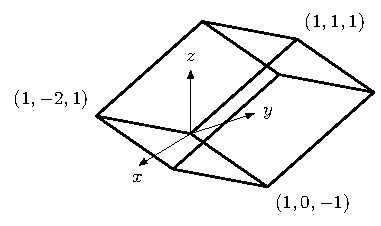
\includegraphics[width=0.6\textwidth]{figuras/paralelepipedo-tres-vectores.pdf}
        \caption{Paralelepípedo determinado por tres vectores en $\R^3$.}
    \end{figure}

    En nuestra discusión anterior sobre el significado geométrico del determinante formado a partir de los vectores en una base ordenada para $\R^2$, también vimos que este determinante es positivo si y solo si la base induce un sistema de coordenadas de mano derecha. Una afirmación similar es cierta en $\R^n$. Específicamente, si $\gamma$ es cualquier base ordenada para $\R^n$ y $\beta$ es la base ordenada estándar para $\R^n$, entonces $\gamma$ induce un sistema de coordenadas de mano derecha si y solo si $\det(Q)>0$, donde $Q$ es la matriz de cambio de coordenadas que cambia coordenadas $\gamma$ a coordenadas $\beta$. Así, por ejemplo,
    \begin{equation*}
        \gamma=\left\{\begin{pmatrix}1\\1\\0\end{pmatrix},\begin{pmatrix}1\\-1\\0\end{pmatrix},\begin{pmatrix}0\\0\\1\end{pmatrix}\right\}
    \end{equation*}
    induce un sistema de coordenadas de mano izquierda en $\R^3$ porque
    \begin{equation*}
        \det\begin{pmatrix}1&1&0\\1&-1&0\\0&0&1\end{pmatrix}=-2<0,
    \end{equation*}
    mientras que
    \begin{equation*}
        \gamma'=\left\{\begin{pmatrix}1\\2\\0\end{pmatrix},\begin{pmatrix}-2\\1\\0\end{pmatrix},\begin{pmatrix}0\\0\\1\end{pmatrix}\right\}
    \end{equation*}
    induce un sistema de coordenadas de mano derecha en $\R^3$ porque
    \begin{equation*}
        \det\begin{pmatrix}1&-2&0\\2&1&0\\0&0&1\end{pmatrix}=5>0.
    \end{equation*}

    Más generalmente, si $\beta$ y $\gamma$ son dos bases ordenadas para $\R^n$, entonces los sistemas de coordenadas inducidos por $\beta$ y $\gamma$ tienen la misma \textbf{orientación} (ambos de mano derecha o ambos de mano izquierda) si y solo si $\det(Q)>0$, donde $Q$ es la matriz de cambio de coordenadas que cambia coordenadas $\gamma$ a coordenadas $\beta$.

    \begin{ejercicio}
        Etiquete las siguientes afirmaciones como verdaderas o falsas.
        \begin{enumerate}[label=(\alph*)]
            \item Si $E$ es una matriz elemental, entonces $\det(E)=\pm1$.
            \item Para cualesquiera $A,B\in M_{n\times n}(F)$, $\det(AB)=\det(A)\cdot\det(B)$.
            \item Una matriz $M\in M_{n\times n}(F)$ es invertible si y solo si $\det(M)=0$.
            \item Una matriz $M\in M_{n\times n}(F)$ tiene rango $n$ si y solo si $\det(M)\neq0$.
            \item Para cualquier $A\in M_{n\times n}(F)$, $\det(A^t)=-\det(A)$.
            \item El determinante de una matriz cuadrada puede evaluarse mediante expansión por cofactores a lo largo de cualquier columna.
            \item Todo sistema de $n$ ecuaciones lineales en $n$ incógnitas puede resolverse mediante la regla de Cramer.
            \item Sea $Ax=b$ la forma matricial de un sistema de $n$ ecuaciones lineales en $n$ incógnitas, donde $x=(x_1,x_2,\dots,x_n)^t$. Si $\det(A)\neq0$ y $M_k$ es la matriz $n\times n$ obtenida de $A$ al reemplazar la columna $k$ de $A$ por $b^t$, entonces la única solución de $Ax=b$ es
            \begin{equation*}
                x_k=\frac{\det(M_k)}{\det(A)}\qquad\text{para }k=1,2,\dots,n.
            \end{equation*}
        \end{enumerate}
    \end{ejercicio}

    En los Ejercicios~2 al~7, use la regla de Cramer para resolver el sistema de ecuaciones lineales dado.

    \begin{ejercicio}
        $\begin{aligned}a_{11}x_1+a_{12}x_2&=b_1\\a_{21}x_1+a_{22}x_2&=b_2\end{aligned}$\\ donde $a_{11}a_{22}-a_{12}a_{21}\neq0$
    \end{ejercicio}

    \begin{ejercicio}
        $\begin{aligned}2x_1+\;\,x_2-3x_3&=5\\x_1-2x_2+\;\,x_3&=10\\3x_1+4x_2-2x_3&=0\end{aligned}$
    \end{ejercicio}

    \begin{ejercicio}
        $\begin{aligned}x_1-\;\,x_2+4x_3&=-4\\-8x_1+3x_2+\;\,x_3&=8\\2x_1-\;\,x_2+\;\,x_3&=0\end{aligned}$
    \end{ejercicio}

    \begin{ejercicio}
        $\begin{aligned}x_1-2x_2+\;\,x_3&=1\\2x_1+\;\,x_2-3x_3&=1\\3x_1+\;\,x_2+\;\,x_3&=4\end{aligned}$
    \end{ejercicio}

    \begin{ejercicio}
        $\begin{aligned}x_1-\;\,x_2+4x_3&=-2\\-8x_1+3x_2+\;\,x_3&=0\\2x_1-\;\,x_2+\;\,x_3&=6\end{aligned}$
    \end{ejercicio}

    \begin{ejercicio}
        $\begin{aligned}-2x_1-\;\,x_2\qquad{}&=12\\x_1+2x_2+x_3&=-8\\3x_1+\;\,x_2+x_3&=4\end{aligned}$
    \end{ejercicio}

    \begin{ejercicio}
        Use el Teorema~4.8 para probar un resultado análogo al Teorema~4.3, pero para columnas.
    \end{ejercicio}

    \begin{ejercicio}
        Pruebe que una matriz triangular superior $n\times n$ es invertible si y solo si todas sus entradas diagonales son no nulas.
    \end{ejercicio}

    \begin{ejercicio}
        Una matriz $M\in M_{n\times n}(\C)$ se llama \textbf{nilpotente} si, para algún entero positivo $k$, $M^k=O$, donde $O$ es la matriz cero $n\times n$. Pruebe que, si $M$ es nilpotente, entonces $\det(M)=0$.
    \end{ejercicio}

    \begin{ejercicio}
        Una matriz $M\in M_{n\times n}(\C)$ se llama \textbf{antisimétrica} si $M^t=-M$. Pruebe que, si $M$ es antisimétrica y $n$ es impar, entonces $M$ no es invertible. ¿Qué sucede si $n$ es par?
    \end{ejercicio}

    \begin{ejercicio}
        Una matriz $Q\in M_{n\times n}(\R)$ se llama \textbf{ortogonal} si $QQ^t=I$. Pruebe que, si $Q$ es ortogonal, entonces $\det(Q)=\pm1$.
    \end{ejercicio}

    \begin{ejercicio}
        Para $M\in M_{n\times n}(\C)$, sea $\overline{M}$ la matriz tal que $(\overline{M})_{ij}=\overline{M_{ij}}$ para todos $i,j$, donde $\overline{M_{ij}}$ es el conjugado complejo de $M_{ij}$.
        \begin{enumerate}[label=(\alph*)]
            \item Pruebe que $\det(\overline{M})=\overline{\det(M)}$.
            \item Una matriz $Q\in M_{n\times n}(\C)$ se llama \textbf{unitaria} si $QQ^*=I$, donde $Q^*=\overline{Q}^t$. Pruebe que, si $Q$ es una matriz unitaria, entonces $|\det(Q)|=1$.
        \end{enumerate}
    \end{ejercicio}

    \begin{ejercicio}
        Sea $\beta=\{u_1,u_2,\dots,u_n\}$ un subconjunto de $F^n$ que contiene $n$ vectores distintos, y sea $B$ la matriz en $M_{n\times n}(F)$ que tiene a $u_j$ como columna $j$. Pruebe que $\beta$ es una base para $F^n$ si y solo si $\det(B)\neq0$.
    \end{ejercicio}

    \begin{ejercicio}
        Pruebe que, si $A,B\in M_{n\times n}(F)$ son semejantes, entonces $\det(A)=\det(B)$.
    \end{ejercicio}

    \begin{ejercicio}
        Use determinantes para probar que, si $A,B\in M_{n\times n}(F)$ son tales que $AB=I$, entonces $A$ es invertible (y por tanto $B=A^{-1}$).
    \end{ejercicio}

    \begin{ejercicio}
        Sean $A,B\in M_{n\times n}(F)$ tales que $AB=-BA$. Pruebe que, si $n$ es impar y $F$ no es un campo de característica dos, entonces $A$ o $B$ no es invertible.
    \end{ejercicio}

    \begin{ejercicio}
        Complete la demostración del Teorema~4.7 mostrando que, si $A$ es una matriz elemental de tipo 2 o de tipo 3, entonces $\det(AB)=\det(A)\cdot\det(B)$.
    \end{ejercicio}

    \begin{ejercicio}
        Una matriz $A\in M_{n\times n}(F)$ se llama \textbf{triangular inferior} si $A_{ij}=0$ para $1\leq i<j\leq n$. Suponga que $A$ es una matriz triangular inferior. Describa $\det(A)$ en términos de las entradas de $A$.
    \end{ejercicio}

    \begin{ejercicio}
        Suponga que $M\in M_{n\times n}(F)$ puede escribirse en la forma
        \begin{equation*}
            M=\begin{pmatrix}A&B\\O&I\end{pmatrix},
        \end{equation*}
        donde $A$ es una matriz cuadrada. Pruebe que $\det(M)=\det(A)$.
    \end{ejercicio}

    \begin{ejercicio}
        Pruebe que, si $M\in M_{n\times n}(F)$ puede escribirse en la forma
        \begin{equation*}
            M=\begin{pmatrix}A&B\\O&C\end{pmatrix},
        \end{equation*}
        donde $A$ y $C$ son matrices cuadradas, entonces $\det(M)=\det(A)\cdot\det(C)$.
    \end{ejercicio}

    \begin{ejercicio}
        Sea $T:P_n(F)\to F^{n+1}$ la transformación lineal definida en el Ejercicio~100 de la Sección~2.4 por $T(f)=\big(f(c_0),f(c_1),\dots,f(c_n)\big)$, donde $c_0,c_1,\dots,c_n$ son escalares distintos en un campo infinito $F$. Sea $\beta$ la base ordenada estándar para $P_n(F)$ y $\gamma$ la base ordenada estándar para $F^{n+1}$. Sea $M=[T]_\beta^\gamma$.
        \begin{enumerate}[label=(\alph*)]
            \item Muestre que $M$ tiene la forma
            \begin{equation*}
                \begin{pmatrix}1&c_0&c_0^2&\cdots&c_0^n\\1&c_1&c_1^2&\cdots&c_1^n\\\vdots&\vdots&&&\vdots\\1&c_n&c_n^2&\cdots&c_n^n\end{pmatrix}.
            \end{equation*}
            Una matriz con esta forma se llama una \textbf{matriz de Vandermonde}.
            \item Use el Ejercicio~100 de la Sección~2.4 para probar que $\det(M)\neq0$.
            \item Pruebe que
            \begin{equation*}
                \det(M)=\prod_{0\leq i<j\leq n}(c_j-c_i),
            \end{equation*}
            el producto de todos los términos de la forma $c_j-c_i$ para $0\leq i<j\leq n$.
        \end{enumerate}
    \end{ejercicio}

    \begin{ejercicio}
        Sea $A\in M_{n\times n}(F)$ no nula. Para cualquier $m$ ($1\leq m\leq n$), una \textbf{submatriz} $m\times m$ se obtiene al eliminar cualesquiera $n-m$ renglones y $n-m$ columnas de $A$.
        \begin{enumerate}[label=(\alph*)]
            \item Sea $k$ ($1\leq k\leq n$) el mayor entero tal que alguna submatriz $k\times k$ tiene determinante no nulo. Pruebe que $\rg(A)=k$.
            \item Recíprocamente, suponga que $\rg(A)=k$. Pruebe que existe una submatriz $k\times k$ con determinante no nulo.
        \end{enumerate}
    \end{ejercicio}

    \begin{ejercicio}
        Sea $A\in M_{n\times n}(F)$ de la forma
        \begin{equation*}
            A=\begin{pmatrix}0&0&0&\cdots&0&a_0\\-1&0&0&\cdots&0&a_1\\0&-1&0&\cdots&0&a_2\\\vdots&\vdots&\vdots&&\vdots&\vdots\\0&0&0&\cdots&-1&a_{n-1}\end{pmatrix}.
        \end{equation*}
        Calcule $\det(A+tI)$, donde $I$ es la matriz identidad $n\times n$.
    \end{ejercicio}

    \begin{ejercicio}
        Sea $c_{jk}$ el cofactor del renglón $j$, columna $k$ de la matriz $A\in M_{n\times n}(F)$.
        \begin{enumerate}[label=(\alph*)]
            \item Pruebe que, si $B$ es la matriz obtenida de $A$ al reemplazar la columna $k$ por $e_j$, entonces $\det(B)=c_{jk}$.
            \item Muestre que, para $1\leq j\leq n$, tenemos
            \begin{equation*}
                A\begin{pmatrix}c_{j1}\\c_{j2}\\\vdots\\c_{jn}\end{pmatrix}=\det(A)\cdot e_j.
            \end{equation*}
            \textit{Sugerencia:} Aplique la regla de Cramer a $Ax=e_j$.
            \item Deduzca que, si $C$ es la matriz $n\times n$ tal que $C_{ij}=c_{ji}$, entonces $AC=[\det(A)]I$.
            \item Muestre que, si $\det(A)\neq0$, entonces $A^{-1}=[\det(A)]^{-1}C$.
        \end{enumerate}
    \end{ejercicio}

    La siguiente definición se usa en los Ejercicios~26 y~27.

    \begin{definicion}[Adjunta clásica]
        La \textbf{adjunta clásica} de una matriz cuadrada $A$ es la transpuesta de la matriz cuya entrada $ij$ es el cofactor $ij$ de $A$.
    \end{definicion}

    \begin{ejercicio}
        Halle la adjunta clásica de cada una de las siguientes matrices.
        \begin{multicols}{2}
        \begin{enumerate}[label=(\alph*)]
            \item $\begin{pmatrix}A_{11}&A_{12}\\A_{21}&A_{22}\end{pmatrix}$
            \item $\begin{pmatrix}4&0&0\\0&4&0\\0&0&4\end{pmatrix}$
            \item $\begin{pmatrix}-4&0&0\\0&2&0\\0&0&5\end{pmatrix}$
            \item $\begin{pmatrix}3&6&7\\0&4&8\\0&0&5\end{pmatrix}$
            \item $\begin{pmatrix}1-i&0&0\\4&3i&0\\2i&1+4i&-1\end{pmatrix}$
            \item $\begin{pmatrix}7&1&4\\6&-3&0\\-3&5&-2\end{pmatrix}$
            \item $\begin{pmatrix}-1&2&5\\8&0&-3\\4&6&1\end{pmatrix}$
            \item $\begin{pmatrix}3&2+i&0\\-1+i&0&i\\0&1&3-2i\end{pmatrix}$
        \end{enumerate}
        \end{multicols}
    \end{ejercicio}

    \begin{ejercicio}
        Sea $C$ la adjunta clásica de $A\in M_{n\times n}(F)$. Pruebe las siguientes afirmaciones.
        \begin{enumerate}[label=(\alph*)]
            \item $\det(C)=[\det(A)]^{n-1}$.
            \item $C^t$ es la adjunta clásica de $A^t$.
            \item Si $A$ es una matriz triangular superior invertible, entonces $C$ y $A^{-1}$ son ambas matrices triangulares superiores.
        \end{enumerate}
    \end{ejercicio}

    \begin{ejercicio}
        Sean $y_1,y_2,\dots,y_n$ funciones linealmente independientes en $\mathcal{C}^\infty$. Para cada $y\in\mathcal{C}^\infty$, defina $\mathsf{T}(y)\in\mathcal{C}^\infty$ por
        \begin{equation*}
            [\mathsf{T}(y)](t)=\det\begin{pmatrix}y(t)&y_1(t)&y_2(t)&\cdots&y_n(t)\\y'(t)&y_1'(t)&y_2'(t)&\cdots&y_n'(t)\\\vdots&\vdots&\vdots&&\vdots\\y^{(n)}(t)&y_1^{(n)}(t)&y_2^{(n)}(t)&\cdots&y_n^{(n)}(t)\end{pmatrix}.
        \end{equation*}
        El determinante anterior se llama el \textbf{Wronskiano} de $y,y_1,\dots,y_n$.
        \begin{enumerate}[label=(\alph*)]
            \item Pruebe que $\mathsf{T}:\mathcal{C}^\infty\to\mathcal{C}^\infty$ es una transformación lineal.
            \item Pruebe que $\ker(\mathsf{T})=\gen{\{y_1,y_2,\dots,y_n\}}$.
        \end{enumerate}
    \end{ejercicio}

    \section{Resumen: hechos importantes sobre determinantes}

    En esta sección resumimos las propiedades importantes del determinante que se necesitan para el resto de estas notas. Los resultados contenidos en esta sección se dedujeron en las Secciones~4.2 y 4.3; en consecuencia, los hechos presentados aquí se enuncian sin demostración.

    El \textbf{determinante} de una matriz $A$ de tamaño $n\times n$ con entradas en un campo $F$ es un escalar en $F$, denotado $\det(A)$ o $|A|$, y puede calcularse de la siguiente manera:
    \begin{enumerate}
        \item Si $A$ es $1\times1$, entonces $\det(A)=A_{11}$, la única entrada de $A$.
        \item Si $A$ es $2\times2$, entonces $\det(A)=A_{11}A_{22}-A_{12}A_{21}$. Por ejemplo,
        \begin{equation*}
            \det\begin{pmatrix}-1&2\\5&3\end{pmatrix}=(-1)(3)-(2)(5)=-13.
        \end{equation*}
        \item Si $A$ es $n\times n$ para $n>2$,
        \begin{equation*}
            \det(A)=\sum_{j=1}^n(-1)^{i+j}A_{ij}\cdot\det(\widetilde{A}_{ij})
        \end{equation*}
        (si el determinante se evalúa mediante las entradas del renglón $i$ de $A$) o
        \begin{equation*}
            \det(A)=\sum_{i=1}^n(-1)^{i+j}A_{ij}\cdot\det(\widetilde{A}_{ij})
        \end{equation*}
        (si el determinante se evalúa mediante las entradas de la columna $j$ de $A$), donde $\widetilde{A}_{ij}$ es la matriz $(n-1)\times(n-1)$ obtenida al eliminar el renglón $i$ y la columna $j$ de $A$.
    \end{enumerate}
    En las fórmulas anteriores, el escalar $(-1)^{i+j}\det(\widetilde{A}_{ij})$ se llama el \textbf{cofactor} de la entrada del renglón $i$, columna $j$ de $A$. En este lenguaje, el determinante de $A$ se evalúa como la suma de términos obtenidos al multiplicar cada entrada de algún renglón o columna de $A$ por el cofactor de dicha entrada. Así $\det(A)$ se expresa en términos de $n$ determinantes de matrices $(n-1)\times(n-1)$. Estos determinantes se evalúan a su vez en términos de determinantes de matrices $(n-2)\times(n-2)$, y así sucesivamente, hasta obtener determinantes de matrices $2\times2$. Los determinantes de las matrices $2\times2$ se evalúan entonces como en el punto 2.

    Consideremos dos ejemplos de esta técnica al evaluar el determinante de la matriz $4\times4$
    \begin{equation*}
        A=\begin{pmatrix}2&1&1&5\\1&1&-4&-1\\2&0&-3&1\\3&6&1&2\end{pmatrix}.
    \end{equation*}
    Para evaluar el determinante de $A$ expandiendo a lo largo del cuarto renglón, debemos conocer los cofactores de cada entrada de ese renglón. El cofactor de $A_{41}=3$ es $(-1)^{4+1}\det(B)$, donde
    \begin{equation*}
        B=\begin{pmatrix}1&1&5\\1&-4&-1\\0&-3&1\end{pmatrix}.
    \end{equation*}
    Evaluemos este determinante expandiendo a lo largo de la primera columna. Tenemos
    \begin{align*}
        \det(B)&=(-1)^{1+1}(1)\det\begin{pmatrix}-4&-1\\-3&1\end{pmatrix}+(-1)^{2+1}(1)\det\begin{pmatrix}1&5\\-3&1\end{pmatrix}\\
        &\qquad{}+(-1)^{3+1}(0)\det\begin{pmatrix}1&5\\-4&-1\end{pmatrix}\\
        &=1(1)\big[(-4)(1)-(-1)(-3)\big]+(-1)(1)\big[(1)(1)-(5)(-3)\big]+0\\
        &=1(-7)-1(16)+0\\
        &=-23.
    \end{align*}
    Así el cofactor de $A_{41}$ es $(-1)^5(-23)=23$. De manera similar, los cofactores de $A_{42}$, $A_{43}$, y $A_{44}$ son $8$, $11$, y $-13$, respectivamente. Podemos ahora evaluar el determinante de $A$ multiplicando cada entrada del cuarto renglón por su cofactor; esto da
    \begin{equation*}
        \det(A)=3(23)+6(8)+1(11)+2(-13)=102.
    \end{equation*}

    Por comparación, evaluemos también el determinante de $A$ mediante expansión a lo largo de la segunda columna. El lector debe verificar que los cofactores de $A_{12}$, $A_{22}$, y $A_{42}$ son $-14$, $40$, y $8$, respectivamente. Así
    \begin{align*}
        \det(A)&=(-1)^{1+2}(1)\det\begin{pmatrix}1&-4&-1\\2&-3&1\\3&1&2\end{pmatrix}+(-1)^{2+2}(1)\det\begin{pmatrix}2&1&5\\2&-3&1\\3&1&2\end{pmatrix}\\
        &\qquad{}+(-1)^{3+2}(0)\det\begin{pmatrix}2&1&5\\1&-4&-1\\3&1&2\end{pmatrix}+(-1)^{4+2}(6)\det\begin{pmatrix}2&1&5\\1&-4&-1\\2&-3&1\end{pmatrix}\\
        &=14+40+0+48\\
        &=102.
    \end{align*}

    Desde luego, no sorprende que se obtenga de nuevo el valor $102$, ya que el valor del determinante de una matriz cuadrada es independiente de la elección del renglón o columna usado en la expansión.

    Observe que el cálculo de $\det(A)$ es más sencillo al expandir a lo largo de la segunda columna que a lo largo del cuarto renglón. La diferencia es la presencia de un cero en la segunda columna, lo cual hace innecesario evaluar uno de los cofactores (el cofactor de $A_{32}$). Por esta razón, conviene evaluar el determinante de una matriz expandiendo a lo largo de un renglón o columna de la matriz que contenga el mayor número de entradas nulas. De hecho, con frecuencia es útil introducir ceros en la matriz mediante operaciones elementales de renglón antes de calcular el determinante. Esta técnica utiliza las primeras tres propiedades del determinante.

    \subsection*{Propiedades del determinante}
    \begin{enumerate}
        \item Si $B$ es una matriz obtenida al intercambiar cualesquiera dos renglones o al intercambiar cualesquiera dos columnas de una matriz $A$ de tamaño $n\times n$, entonces $\det(B)=-\det(A)$.
        \item Si $B$ es una matriz obtenida al multiplicar cada entrada de algún renglón o columna de una matriz $A$ de tamaño $n\times n$ por un escalar $k$, entonces $\det(B)=k\cdot\det(A)$.
        \item Si $B$ es una matriz obtenida de una matriz $A$ de tamaño $n\times n$ al sumar un múltiplo del renglón $i$ o de la columna $i$ al renglón $j$ o a la columna $j$, para $i\neq j$, entonces $\det(B)=\det(A)$.
    \end{enumerate}

    Como ejemplo del uso de estas tres propiedades al evaluar determinantes, calculemos el determinante de la matriz $4\times4$ $A$ considerada anteriormente. Nuestro procedimiento consiste en introducir ceros en la segunda columna de $A$ empleando la propiedad 3, y luego expandir a lo largo de esa columna. (Las operaciones elementales de renglón usadas aquí consisten en sumar múltiplos del renglón 1 a los renglones 2 y 4.) Este procedimiento produce
    \begin{equation*}
        \det(A)=\det\begin{pmatrix}2&1&1&5\\1&1&-4&-1\\2&0&-3&1\\3&6&1&2\end{pmatrix}
        =\det\begin{pmatrix}2&1&1&5\\-1&0&-5&-6\\2&0&-3&1\\-9&0&-5&-28\end{pmatrix}
        =1\cdot(-1)^{1+2}\det\begin{pmatrix}-1&-5&-6\\2&-3&1\\-9&-5&-28\end{pmatrix}.
    \end{equation*}
    El determinante $3\times3$ resultante puede evaluarse de la misma manera: use operaciones elementales de renglón de tipo 3 para introducir dos ceros en la primera columna, y luego expanda a lo largo de esa columna. Esto resulta en el valor $-102$. Por tanto
    \begin{equation*}
        \det(A)=1\cdot(-1)^{1+2}(-102)=102.
    \end{equation*}

    El lector debe comparar este cálculo de $\det(A)$ con los cálculos anteriores para ver cuánto menos trabajo se requiere cuando se emplean las propiedades 1, 2, y 3.

    En los capítulos que siguen, con frecuencia debemos evaluar el determinante de matrices que tienen formas especiales. Las siguientes dos propiedades del determinante son útiles a este respecto:
    \begin{enumerate}
        \setcounter{enumi}{3}
        \item El determinante de una matriz triangular superior es el producto de sus entradas diagonales. En particular, $\det(I)=1$.
        \item Si dos renglones (o columnas) de una matriz son idénticos, entonces el determinante de la matriz es cero.
    \end{enumerate}

    Como ilustración de la propiedad 4, observe que
    \begin{equation*}
        \det\begin{pmatrix}-3&1&2\\0&4&5\\0&0&-6\end{pmatrix}=(-3)(4)(-6)=72.
    \end{equation*}
    La propiedad 4 proporciona un método eficiente para evaluar el determinante de una matriz:
    \begin{enumerate}[label=(\alph*)]
        \item Use eliminación gaussiana y las propiedades 1, 2, y 3 anteriores para reducir la matriz a una matriz triangular superior.
        \item Calcule el producto de las entradas diagonales.
    \end{enumerate}
    Por ejemplo,
    \begin{equation*}
        \det\begin{pmatrix}1&-1&2&1\\2&-1&-1&4\\-4&5&-10&-6\\3&-2&10&-1\end{pmatrix}
        =\det\begin{pmatrix}1&-1&2&1\\0&1&-5&2\\0&1&-2&-2\\0&1&4&-4\end{pmatrix}
    \end{equation*}
    \begin{equation*}
        =\det\begin{pmatrix}1&-1&2&1\\0&1&-5&2\\0&0&3&-4\\0&0&9&-6\end{pmatrix}
        =\det\begin{pmatrix}1&-1&2&1\\0&1&-5&2\\0&0&3&-4\\0&0&0&6\end{pmatrix}
        =1\cdot1\cdot3\cdot6=18.
    \end{equation*}

    Las siguientes tres propiedades del determinante se usan con frecuencia en capítulos posteriores. De hecho, quizás la propiedad más importante del determinante es que proporciona una caracterización simple de las matrices invertibles. (Véase la propiedad 7.)
    \begin{enumerate}
        \setcounter{enumi}{5}
        \item Para cualesquiera matrices $A,B\in M_{n\times n}(F)$, $\det(AB)=\det(A)\cdot\det(B)$.
        \item Una matriz $A\in M_{n\times n}(F)$ es invertible si y solo si $\det(A)\neq0$. Más aún, si $A$ es invertible, entonces
        \begin{equation*}
            \det(A^{-1})=\frac{1}{\det(A)}.
        \end{equation*}
        \item Para cualquier matriz $A\in M_{n\times n}(F)$, los determinantes de $A$ y de $A^t$ son iguales.
    \end{enumerate}

    Por ejemplo, la propiedad 7 garantiza que la matriz $A$ de la página~232 es invertible porque $\det(A)=102$.

    La última propiedad, enunciada como el Ejercicio~57 de la Sección~4.3, se usa en el Capítulo~5. Es una consecuencia sencilla de las propiedades 6 y 7.
    \begin{enumerate}
        \setcounter{enumi}{8}
        \item Si $A$ y $B$ son matrices semejantes, entonces $\det(A)=\det(B)$.
    \end{enumerate}

    \begin{ejercicio}
        Etiquete las siguientes afirmaciones como verdaderas o falsas.
        \begin{enumerate}[label=(\alph*)]
            \item El determinante de una matriz cuadrada puede calcularse expandiendo la matriz a lo largo de cualquier renglón o columna.
            \item Al evaluar el determinante de una matriz, conviene expandir a lo largo de un renglón o columna que contenga el mayor número de entradas nulas.
            \item Si dos renglones o columnas de $A$ son idénticos, entonces $\det(A)=0$.
            \item Si $B$ es una matriz obtenida al intercambiar dos renglones o dos columnas de $A$, entonces $\det(B)=\det(A)$.
            \item Si $B$ es una matriz obtenida al multiplicar cada entrada de algún renglón o columna de $A$ por un escalar, entonces $\det(B)=\det(A)$.
            \item Si $B$ es una matriz obtenida de $A$ al sumar un múltiplo de algún renglón a otro renglón distinto, entonces $\det(B)=\det(A)$.
            \item El determinante de una matriz triangular superior $n\times n$ es el producto de sus entradas diagonales.
            \item Para cualquier $A\in M_{n\times n}(F)$, $\det(A^t)=-\det(A)$.
            \item Si $A,B\in M_{n\times n}(F)$, entonces $\det(AB)=\det(A)\cdot\det(B)$.
            \item Si $Q$ es una matriz invertible, entonces $\det(Q^{-1})=[\det(Q)]^{-1}$.
            \item Una matriz $Q$ es invertible si y solo si $\det(Q)\neq0$.
        \end{enumerate}
    \end{ejercicio}

    \begin{ejercicio}
        Evalúe el determinante de las siguientes matrices $2\times2$.
        \begin{multicols}{2}
        \begin{enumerate}[label=(\alph*)]
            \item $\begin{pmatrix}4&-5\\2&3\end{pmatrix}$
            \item $\begin{pmatrix}-1&7\\3&8\end{pmatrix}$
            \item $\begin{pmatrix}2+i&-1+3i\\1-2i&3-i\end{pmatrix}$
            \item $\begin{pmatrix}3&4i\\-6i&2i\end{pmatrix}$
        \end{enumerate}
        \end{multicols}
    \end{ejercicio}

    \begin{ejercicio}
        Evalúe el determinante de las siguientes matrices de la manera indicada.
        \begin{multicols}{2}
        \begin{enumerate}[label=(\alph*)]
            \item[(a)] $\begin{pmatrix}0&1&2\\-1&0&-3\\2&3&0\end{pmatrix}$ a lo largo del primer renglón
            \item[(b)] $\begin{pmatrix}1&0&2\\0&1&5\\-1&3&0\end{pmatrix}$ a lo largo de la primera columna
            \item[(c)] $\begin{pmatrix}0&1&2\\-1&0&-3\\2&3&0\end{pmatrix}$ a lo largo de la segunda columna
            \item[(d)] $\begin{pmatrix}1&0&2\\0&1&5\\-1&3&0\end{pmatrix}$ a lo largo del tercer renglón
            \item[(e)] $\begin{pmatrix}0&1+i&2\\-2i&0&1-i\\3&4i&0\end{pmatrix}$ a lo largo del tercer renglón
            \item[(f)] $\begin{pmatrix}i&2+i&0\\-1&3&2i\\0&-1&1-i\end{pmatrix}$ a lo largo de la tercera columna
            \item[(g)] $\begin{pmatrix}0&2&1&3\\1&0&-2&2\\3&-1&0&1\\-1&1&2&0\end{pmatrix}$ a lo largo de la cuarta columna
            \item[(h)] $\begin{pmatrix}1&-1&2&-1\\-3&4&1&-1\\2&-5&-3&8\\-2&6&-4&1\end{pmatrix}$ a lo largo del cuarto renglón
        \end{enumerate}
        \end{multicols}
    \end{ejercicio}

    \begin{ejercicio}
        Evalúe el determinante de las siguientes matrices mediante cualquier método legítimo.
        \begin{multicols}{2}
        \begin{enumerate}[label=(\alph*)]
            \item $\begin{pmatrix}1&2&3\\4&5&6\\7&8&9\end{pmatrix}$
            \item $\begin{pmatrix}-1&3&2\\4&-8&1\\2&2&5\end{pmatrix}$
            \item $\begin{pmatrix}0&1&1\\1&2&-5\\6&-4&3\end{pmatrix}$
            \item $\begin{pmatrix}1&-2&3\\-1&2&-5\\3&-1&2\end{pmatrix}$
            \item $\begin{pmatrix}i&2&-1\\3&1+i&2\\-2i&1&4-i\end{pmatrix}$
            \item $\begin{pmatrix}-1&2+i&3\\1-i&i&1\\3i&2&-1+i\end{pmatrix}$
            \item $\begin{pmatrix}1&0&-2&3\\-3&1&1&2\\0&4&-1&1\\2&3&0&1\end{pmatrix}$
            \item $\begin{pmatrix}1&-2&3&-12\\-5&12&-14&19\\-9&22&-20&31\\-4&9&-14&15\end{pmatrix}$
        \end{enumerate}
        \end{multicols}
    \end{ejercicio}

    \begin{ejercicio}
        Suponga que $M\in M_{n\times n}(F)$ puede escribirse en la forma
        \begin{equation*}
            M=\begin{pmatrix}A&B\\O&I\end{pmatrix},
        \end{equation*}
        donde $A$ es una matriz cuadrada. Pruebe que $\det(M)=\det(A)$.
    \end{ejercicio}

    \begin{ejercicio}
        Pruebe que, si $M\in M_{n\times n}(F)$ puede escribirse en la forma
        \begin{equation*}
            M=\begin{pmatrix}A&B\\O&C\end{pmatrix},
        \end{equation*}
        donde $A$ y $C$ son matrices cuadradas, entonces $\det(M)=\det(A)\cdot\det(C)$.
    \end{ejercicio}

    \section{Una caracterización del determinante}

    En las Secciones~4.2 y 4.3 mostramos que el determinante posee varias propiedades. En esta sección mostramos que tres de estas propiedades caracterizan completamente al determinante; es decir, la única función $\delta:M_{n\times n}(F)\to F$ que tiene estas tres propiedades es el determinante. Esta caracterización del determinante es la que se usó en la Sección~4.1 para establecer la relación entre
    \begin{equation*}
        \det\begin{pmatrix}u\\v\end{pmatrix}
    \end{equation*}
    y el área del paralelogramo determinado por $u$ y $v$. La primera de estas propiedades que caracterizan al determinante es la descrita en el Teorema~4.3 (p.~212).

    \begin{definicion}[Función $n$-lineal]
        Una función $\delta:M_{n\times n}(F)\to F$ se llama una \textbf{función $n$-lineal} si es una función lineal de cada renglón de una matriz $n\times n$ cuando los demás $n-1$ renglones se mantienen fijos, es decir, $\delta$ es $n$-lineal si, para cada $r=1,2,\dots,n$, tenemos
        \begin{equation*}
            \delta\begin{pmatrix}a_1\\\vdots\\a_{r-1}\\u+kv\\a_{r+1}\\\vdots\\a_n\end{pmatrix}
            =\delta\begin{pmatrix}a_1\\\vdots\\a_{r-1}\\u\\a_{r+1}\\\vdots\\a_n\end{pmatrix}
            +k\delta\begin{pmatrix}a_1\\\vdots\\a_{r-1}\\v\\a_{r+1}\\\vdots\\a_n\end{pmatrix}
        \end{equation*}
        siempre que $k$ sea un escalar y $u$, $v$, y cada $a_i$ sean vectores en $F^n$.
    \end{definicion}

    \begin{ejemplo}
        La función $\delta:M_{n\times n}(F)\to F$ definida por $\delta(A)=0$ para cada $A\in M_{n\times n}(F)$ es una función $n$-lineal.
    \end{ejemplo}

    \begin{ejemplo}
        Para $1\leq j\leq n$, definamos $\delta_j:M_{n\times n}(F)\to F$ por $\delta_j(A)=A_{1j}A_{2j}\cdots A_{nj}$ para cada $A\in M_{n\times n}(F)$; es decir, $\delta_j(A)$ es igual al producto de las entradas de la columna $j$ de $A$. Sea $A\in M_{n\times n}(F)$, $a_i=(A_{i1},A_{i2},\dots,A_{in})$, y $v=(b_1,b_2,\dots,b_n)\in F^n$. Entonces cada $\delta_j$ es una función $n$-lineal porque, para cualquier escalar $k$, tenemos
        \begin{align*}
            \delta_j\begin{pmatrix}a_1\\\vdots\\a_{r-1}\\a_r+kv\\a_{r+1}\\\vdots\\a_n\end{pmatrix}
            &=A_{1j}\cdots A_{(r-1)j}(A_{rj}+kb_j)A_{(r+1)j}\cdots A_{nj}\\
            &=A_{1j}\cdots A_{(r-1)j}A_{rj}A_{(r+1)j}\cdots A_{nj}+A_{1j}\cdots A_{(r-1)j}(kb_j)A_{(r+1)j}\cdots A_{nj}\\
            &=A_{1j}\cdots A_{(r-1)j}A_{rj}A_{(r+1)j}\cdots A_{nj}+k\big(A_{1j}\cdots A_{(r-1)j}b_jA_{(r+1)j}\cdots A_{nj}\big)\\
            &=\delta_j\begin{pmatrix}a_1\\\vdots\\a_{r-1}\\a_r\\a_{r+1}\\\vdots\\a_n\end{pmatrix}
            +k\delta_j\begin{pmatrix}a_1\\\vdots\\a_{r-1}\\v\\a_{r+1}\\\vdots\\a_n\end{pmatrix}.
        \end{align*}
    \end{ejemplo}

    \begin{ejemplo}
        La función $\delta:M_{n\times n}(F)\to F$ definida para cada $A\in M_{n\times n}(F)$ por $\delta(A)=A_{11}A_{22}\cdots A_{nn}$ (es decir, $\delta(A)$ es igual al producto de las entradas diagonales de $A$) es una función $n$-lineal.
    \end{ejemplo}

    \begin{ejemplo}
        La función $\delta:M_{n\times n}(\R)\to\R$ definida para cada $A\in M_{n\times n}(\R)$ por $\delta(A)=\Tr(A)$ no es una función $n$-lineal para $n\geq2$. Pues si $I$ es la matriz identidad $n\times n$ y $A$ es la matriz obtenida al multiplicar el primer renglón de $I$ por $2$, entonces
        \begin{equation*}
            \delta(A)=n+1\neq2n=2\cdot\delta(I).
        \end{equation*}
    \end{ejemplo}

    El Teorema~4.3 (p.~212) afirma que el determinante es una función $n$-lineal. Para nuestros propósitos, este es el ejemplo más importante de una función $n$-lineal. Introducimos ahora la segunda de las propiedades usadas en la caracterización del determinante.

    \begin{definicion}[Función alternante]
        Una función $n$-lineal $\delta:M_{n\times n}(F)\to F$ se llama \textbf{alternante} si, para cada $A\in M_{n\times n}(F)$, tenemos $\delta(A)=0$ siempre que dos renglones adyacentes de $A$ sean idénticos.
    \end{definicion}

    \begin{teorema}
        Sea $\delta:M_{n\times n}(F)\to F$ una función alternante $n$-lineal.
        \begin{enumerate}[label=(\alph*)]
            \item Si $A\in M_{n\times n}(F)$ y $B$ es una matriz obtenida de $A$ al intercambiar cualesquiera dos renglones de $A$, entonces $\delta(B)=-\delta(A)$.
            \item Si $A\in M_{n\times n}(F)$ tiene dos renglones idénticos, entonces $\delta(A)=0$.
        \end{enumerate}
    \end{teorema}
    \begin{proof}
        (a) Sea $A\in M_{n\times n}(F)$, y sea $B$ la matriz obtenida de $A$ al intercambiar los renglones $r$ y $s$, donde $r<s$. Establecemos primero el resultado en el caso en que $s=r+1$. Como $\delta:M_{n\times n}(F)\to F$ es una función $n$-lineal que es alternante, tenemos
        \begin{align*}
            0&=\delta\begin{pmatrix}a_1\\\vdots\\a_r+a_{r+1}\\a_r+a_{r+1}\\\vdots\\a_n\end{pmatrix}
            =\delta\begin{pmatrix}a_1\\\vdots\\a_r\\a_r+a_{r+1}\\\vdots\\a_n\end{pmatrix}
            +\delta\begin{pmatrix}a_1\\\vdots\\a_{r+1}\\a_r+a_{r+1}\\\vdots\\a_n\end{pmatrix}\\
            &=\delta\begin{pmatrix}a_1\\\vdots\\a_r\\a_r\\\vdots\\a_n\end{pmatrix}
            +\delta\begin{pmatrix}a_1\\\vdots\\a_r\\a_{r+1}\\\vdots\\a_n\end{pmatrix}
            +\delta\begin{pmatrix}a_1\\\vdots\\a_{r+1}\\a_r\\\vdots\\a_n\end{pmatrix}
            +\delta\begin{pmatrix}a_1\\\vdots\\a_{r+1}\\a_{r+1}\\\vdots\\a_n\end{pmatrix}\\
            &=0+\delta(A)+\delta(B)+0.
        \end{align*}
        Así $\delta(B)=-\delta(A)$.

        A continuación supongamos que $s>r+1$, y sean los renglones de $A$ $a_1,a_2,\dots,a_n$. Comenzando con $a_r$, intercambiamos sucesivamente $a_r$ con el renglón que le sigue hasta que los renglones queden en la sucesión
        \begin{equation*}
            a_1,a_2,\dots,a_{r-1},a_{r+1},\dots,a_s,a_r,a_{s+1},\dots,a_n.
        \end{equation*}
        En total se necesitan $s-r$ intercambios de renglones adyacentes para producir esta sucesión. Luego, intercambiamos sucesivamente $a_s$ con el renglón que lo precede hasta que los renglones queden en el orden
        \begin{equation*}
            a_1,a_2,\dots,a_{r-1},a_s,a_{r+1},\dots,a_{s-1},a_r,a_{s+1},\dots,a_n.
        \end{equation*}
        Este proceso requiere $s-r-1$ intercambios adicionales de renglones adyacentes, y produce la matriz $B$. Se sigue del párrafo anterior que
        \begin{equation*}
            \delta(B)=(-1)^{(s-r)+(s-r-1)}\delta(A)=-\delta(A).
        \end{equation*}

        (b) Supongamos que los renglones $r$ y $s$ de $A\in M_{n\times n}(F)$ son idénticos, donde $r<s$. Si $s=r+1$, entonces $\delta(A)=0$ porque $\delta$ es alternante y dos renglones adyacentes de $A$ son idénticos. Si $s>r+1$, sea $B$ la matriz obtenida de $A$ al intercambiar los renglones $r+1$ y $s$. Entonces $\delta(B)=0$ porque dos renglones adyacentes de $B$ son idénticos. Pero $\delta(B)=-\delta(A)$ por (a). De donde $\delta(A)=0$.
    \end{proof}

    \begin{corolario}
        Sea $\delta:M_{n\times n}(F)\to F$ una función alternante $n$-lineal. Si $B$ es una matriz obtenida de $A\in M_{n\times n}(F)$ al sumar un múltiplo de algún renglón de $A$ a otro renglón, entonces $\delta(B)=\delta(A)$.
    \end{corolario}
    \begin{proof}
        Sea $B$ obtenida de $A\in M_{n\times n}(F)$ al sumar $k$ veces el renglón $i$ de $A$ al renglón $j$, donde $j\neq i$, y sea $C$ obtenida de $A$ al reemplazar el renglón $j$ de $A$ por el renglón $i$ de $A$. Los renglones de $A$, $B$, y $C$ son idénticos excepto por el renglón $j$. Más aún, el renglón $j$ de $B$ es la suma del renglón $j$ de $A$ y $k$ veces el renglón $j$ de $C$. Como $\delta$ es una función $n$-lineal y $C$ tiene dos renglones idénticos, se sigue que
        \begin{equation*}
            \delta(B)=\delta(A)+k\delta(C)=\delta(A)+k\cdot0=\delta(A).
        \end{equation*}
    \end{proof}

    El siguiente resultado se sigue ahora como en la demostración del corolario al Teorema~4.6 (p.~216).

    \begin{corolario}
        Sea $\delta:M_{n\times n}(F)\to F$ una función alternante $n$-lineal. Si $M\in M_{n\times n}(F)$ tiene rango menor que $n$, entonces $\delta(M)=0$.
    \end{corolario}
    \begin{proof}
        Si el rango de $M$ es menor que $n$, entonces los renglones $a_1,a_2,\dots,a_n$ de $M$ son linealmente dependientes por el Ejercicio~91 de la Sección~1.5. Así algún renglón de $M$, digamos el renglón $r$, es una combinación lineal de los demás renglones. Por tanto existen escalares $c_i$ tales que
        \begin{equation*}
            a_r=c_1a_1+\cdots+c_{r-1}a_{r-1}+c_{r+1}a_{r+1}+\cdots+c_na_n.
        \end{equation*}
        Sea $N$ la matriz obtenida de $M$ al sumar $-c_i$ veces el renglón $i$ a el renglón $r$ para cada $i\neq r$. Por el corolario~1, $\delta(N)=\delta(M)$. Pero el renglón $r$ de $N$ está formado enteramente por ceros; escribiendo este renglón como $0=0+1\cdot0$ y aplicando la $n$-linealidad de $\delta$ al renglón $r$ (como en la demostración del corolario al Teorema~4.3), obtenemos $\delta(N)=2\delta(N)$, de donde $\delta(N)=0$. Por tanto $\delta(M)=\delta(N)=0$.
    \end{proof}

    \begin{corolario}
        Sea $\delta:M_{n\times n}(F)\to F$ una función alternante $n$-lineal, y sean $E_1$, $E_2$, y $E_3$ en $M_{n\times n}(F)$ matrices elementales de tipos 1, 2, y 3, respectivamente. Supongamos que $E_2$ se obtiene al multiplicar algún renglón de $I$ por el escalar no nulo $k$. Entonces $\delta(E_1)=-\delta(I)$, $\delta(E_2)=k\cdot\delta(I)$, y $\delta(E_3)=\delta(I)$.
    \end{corolario}
    \begin{proof}
        Como $E_1$ se obtiene al intercambiar dos renglones de $I$, el inciso (a) del teorema anterior (aplicado a $A=I$) da $\delta(E_1)=-\delta(I)$.

        Como $E_2$ se obtiene al multiplicar algún renglón de $I$ por el escalar no nulo $k$, la $n$-linealidad de $\delta$ (aplicada al renglón correspondiente de $I$, con $u=0$ y $v$ igual a dicho renglón) da $\delta(E_2)=k\cdot\delta(I)$.

        Como $E_3$ se obtiene al sumar un múltiplo de algún renglón de $I$ a otro renglón, el corolario~1 (aplicado a $A=I$) da $\delta(E_3)=\delta(I)$.
    \end{proof}

    Deseamos mostrar que, bajo ciertas circunstancias, la única función alternante $n$-lineal $\delta:M_{n\times n}(F)\to F$ es el determinante, es decir, $\delta(A)=\det(A)$ para toda $A\in M_{n\times n}(F)$. En vista del teorema anterior y del corolario~3, y de los hechos de la página~223 sobre el determinante de una matriz elemental, esto puede ocurrir solo si $\delta(I)=1$. Por tanto la tercera condición que se usa en la caracterización del determinante es que el determinante de la matriz identidad $n\times n$ es $1$. Antes de poder establecer la caracterización deseada del determinante, debemos primero mostrar que una función alternante $n$-lineal $\delta$ tal que $\delta(I)=1$ es una función multiplicativa. La demostración de este resultado es idéntica a la demostración del Teorema~4.7 (p.~223), y así se omite.

    \begin{teorema}
        Sea $\delta:M_{n\times n}(F)\to F$ una función alternante $n$-lineal tal que $\delta(I)=1$. Para cualesquiera $A,B\in M_{n\times n}(F)$, tenemos $\delta(AB)=\delta(A)\cdot\delta(B)$.
    \end{teorema}

    \begin{teorema}
        Si $\delta:M_{n\times n}(F)\to F$ es una función alternante $n$-lineal tal que $\delta(I)=1$, entonces $\delta(A)=\det(A)$ para toda $A\in M_{n\times n}(F)$.
    \end{teorema}
    \begin{proof}
        Sea $\delta:M_{n\times n}(F)\to F$ una función alternante $n$-lineal tal que $\delta(I)=1$, y sea $A\in M_{n\times n}(F)$. Si $A$ tiene rango menor que $n$, entonces por el corolario~2 al teorema anterior, $\delta(A)=0$. Como el corolario al Teorema~4.6 (p.~217) da $\det(A)=0$, tenemos $\delta(A)=\det(A)$ en este caso.

        Si, por otro lado, $A$ tiene rango $n$, entonces $A$ es invertible y por tanto es el producto de matrices elementales (Corolario~3 al Teorema~3.6, p.~159), digamos $A=E_m\cdots E_2E_1$. Como $\delta(I)=1$, se sigue del corolario~3 al teorema anterior y de los hechos de la página~223 que $\delta(E)=\det(E)$ para cada matriz elemental $E$. De donde, por el teorema anterior y el Teorema~4.7 (p.~223), tenemos
        \begin{align*}
            \delta(A)&=\delta(E_m\cdots E_2E_1)\\
            &=\delta(E_m)\cdot\dots\cdot\delta(E_2)\cdot\delta(E_1)\\
            &=\det(E_m)\cdot\dots\cdot\det(E_2)\cdot\det(E_1)\\
            &=\det(E_m\cdots E_2E_1)\\
            &=\det(A).\qedhere
        \end{align*}
    \end{proof}

    El teorema anterior proporciona la caracterización deseada del determinante: es la única función $\delta:M_{n\times n}(F)\to F$ que es $n$-lineal, es alternante, y tiene la propiedad de que $\delta(I)=1$.

    \begin{ejercicio}
        Etiquete las siguientes afirmaciones como verdaderas o falsas.
        \begin{enumerate}[label=(\alph*)]
            \item Cualquier función $n$-lineal $\delta:M_{n\times n}(F)\to F$ es una transformación lineal.
            \item Cualquier función $n$-lineal $\delta:M_{n\times n}(F)\to F$ es una función lineal de cada renglón de una matriz $n\times n$ cuando los demás $n-1$ renglones se mantienen fijos.
            \item Si $\delta:M_{n\times n}(F)\to F$ es una función alternante $n$-lineal y la matriz $A\in M_{n\times n}(F)$ tiene dos renglones idénticos, entonces $\delta(A)=0$.
            \item Si $\delta:M_{n\times n}(F)\to F$ es una función alternante $n$-lineal y $B$ se obtiene de $A\in M_{n\times n}(F)$ al intercambiar dos renglones de $A$, entonces $\delta(B)=\delta(A)$.
            \item Existe una única función alternante $n$-lineal $\delta:M_{n\times n}(F)\to F$.
            \item La función $\delta:M_{n\times n}(F)\to F$ definida por $\delta(A)=0$ para toda $A\in M_{n\times n}(F)$ es una función alternante $n$-lineal.
        \end{enumerate}
    \end{ejercicio}

    \begin{ejercicio}
        Determine todas las funciones $1$-lineales $\delta:M_{1\times1}(F)\to F$.
    \end{ejercicio}

    Determine cuáles de las funciones $\delta:M_{3\times3}(F)\to F$ en los Ejercicios~3 al~10 son funciones $3$-lineales. Justifique cada respuesta.

    \begin{ejercicio}
        $\delta(A)=k$, donde $k$ es cualquier escalar no nulo.
    \end{ejercicio}

    \begin{ejercicio}
        $\delta(A)=A_{22}$.
    \end{ejercicio}

    \begin{ejercicio}
        $\delta(A)=A_{11}A_{23}A_{32}$.
    \end{ejercicio}

    \begin{ejercicio}
        $\delta(A)=A_{11}+A_{23}+A_{32}$.
    \end{ejercicio}

    \begin{ejercicio}
        $\delta(A)=A_{11}A_{21}A_{32}$.
    \end{ejercicio}

    \begin{ejercicio}
        $\delta(A)=A_{11}A_{31}A_{32}$.
    \end{ejercicio}

    \begin{ejercicio}
        $\delta(A)=A_{11}^2A_{22}^2A_{33}^2$.
    \end{ejercicio}

    \begin{ejercicio}
        $\delta(A)=A_{11}A_{22}A_{33}-A_{11}A_{21}A_{32}$.
    \end{ejercicio}

    \begin{ejercicio}
        Pruebe los Corolarios~2 y 3 del teorema de esta sección sobre funciones alternantes $n$-lineales.
    \end{ejercicio}

    \begin{ejercicio}
        Pruebe el teorema sobre la multiplicatividad de una función alternante $n$-lineal $\delta$ tal que $\delta(I)=1$.
    \end{ejercicio}

    \begin{ejercicio}
        Pruebe que $\det:M_{2\times2}(F)\to F$ es una función $2$-lineal de las \textit{columnas} de una matriz.
    \end{ejercicio}

    \begin{ejercicio}
        Sean $a,b,c,d\in F$. Pruebe que la función $\delta:M_{2\times2}(F)\to F$ definida por $\delta(A)=A_{11}A_{22}a+A_{11}A_{21}b+A_{12}A_{22}c+A_{12}A_{21}d$ es una función $2$-lineal.
    \end{ejercicio}

    \begin{ejercicio}
        Pruebe que $\delta:M_{2\times2}(F)\to F$ es una función $2$-lineal si y solo si tiene la forma
        \begin{equation*}
            \delta(A)=A_{11}A_{22}a+A_{11}A_{21}b+A_{12}A_{22}c+A_{12}A_{21}d
        \end{equation*}
        para algunos escalares $a,b,c,d\in F$.
    \end{ejercicio}

    \begin{ejercicio}
        Pruebe que, si $\delta:M_{n\times n}(F)\to F$ es una función alternante $n$-lineal, entonces existe un escalar $k$ tal que $\delta(A)=k\det(A)$ para toda $A\in M_{n\times n}(F)$.
    \end{ejercicio}

    \begin{ejercicio}
        Pruebe que una combinación lineal de dos funciones $n$-lineales es una función $n$-lineal, donde la suma y el producto por escalar de funciones $n$-lineales se definen como en el Ejemplo~5 de la Sección~1.2 (p.~9).
    \end{ejercicio}

    \begin{ejercicio}
        Pruebe que el conjunto de todas las funciones $n$-lineales sobre un campo $F$ es un espacio vectorial sobre $F$ bajo las operaciones de suma de funciones y producto por escalar definidas como en el Ejemplo~5 de la Sección~1.2 (p.~9).
    \end{ejercicio}

    \begin{ejercicio}
        Sea $\delta:M_{n\times n}(F)\to F$ una función $n$-lineal, y sea $F$ un campo que no tiene característica dos. Pruebe que, si $\delta(B)=-\delta(A)$ siempre que $B$ se obtiene de $A\in M_{n\times n}(F)$ al intercambiar cualesquiera dos renglones de $A$, entonces $\delta(M)=0$ siempre que $M\in M_{n\times n}(F)$ tiene dos renglones idénticos.
    \end{ejercicio}

    \begin{ejercicio}
        Dé un ejemplo que muestre que la implicación del Ejercicio~95 no necesariamente se cumple si $F$ tiene característica dos.
    \end{ejercicio}

    \chapter{Diagonalización}

    Este capítulo trata el problema de la diagonalización. Dado un operador lineal $T$ sobre un espacio vectorial $V$ de dimensión finita, buscamos responder a las siguientes preguntas:

    \begin{enumerate}
        \item ¿Existe una base ordenada $\BB$ de $V$ tal que $[T]_{\BB}$ sea una matriz diagonal?
        \item Si tal base existe, ¿cómo se encuentra?
    \end{enumerate}

    Como los cálculos con matrices diagonales son sencillos, responder afirmativamente a la primera pregunta nos permite entender con claridad cómo actúa $T$ sobre $V$, y responder a la segunda nos permite resolver de forma sencilla muchos problemas que pueden formularse en términos de álgebra lineal.

    Una solución al problema de la diagonalización nos lleva de manera natural a los conceptos de \textbf{valor propio} y \textbf{vector propio}. Además del papel que juegan en el problema de la diagonalización, estos conceptos resultan también útiles en el estudio de operadores que no son diagonalizables.

    \section{Valores propios y vectores propios}

    Consideremos, por ejemplo, la reflexión $T$ de $\R^2$ respecto a la recta $y = 2x$. Tomando como base ordenada $\BB'$ un vector director de la recta y un vector normal a ella, la matriz $[T]_{\BB'}$ resulta diagonal. Esto motiva el siguiente nombre para un operador (o una matriz) que admite una base de este tipo.

    \begin{definicion}[Operador diagonalizable]
        Un operador lineal $T$ sobre un espacio vectorial $V$ de dimensión finita se llama \textbf{diagonalizable} si existe una base ordenada $\BB$ de $V$ tal que $[T]_{\BB}$ es una matriz diagonal. Una matriz cuadrada $A$ se llama \textbf{diagonalizable} si $L_A$ es diagonalizable.
    \end{definicion}

    Queremos determinar cuándo un operador lineal $T$ sobre un espacio vectorial de dimensión finita es diagonalizable y, en caso afirmativo, cómo obtener una base ordenada $\BB = \{v_1, v_2, \dots, v_n\}$ de $V$ tal que $[T]_{\BB}$ sea una matriz diagonal. Observemos que si $D = [T]_{\BB}$ es diagonal, entonces para cada vector $v_j \in \BB$ se tiene
    \begin{equation*}
        T(v_j) = \sum_{i=1}^{n} D_{ij} v_i = D_{jj} v_j = \lambda_j v_j,
    \end{equation*}
    donde $\lambda_j = D_{jj}$.

    Recíprocamente, si $\BB = \{v_1, v_2, \dots, v_n\}$ es una base ordenada de $V$ tal que $T(v_j) = \lambda_j v_j$ para ciertos escalares $\lambda_1, \dots, \lambda_n$, entonces claramente
    \begin{equation*}
        [T]_{\BB} =
        \begin{pmatrix}
            \lambda_1 & 0 & \cdots & 0 \\
            0 & \lambda_2 & \cdots & 0 \\
            \vdots & & \ddots & \vdots \\
            0 & 0 & \cdots & \lambda_n
        \end{pmatrix}.
    \end{equation*}

    En el párrafo anterior, cada vector $v$ de la base $\BB$ satisface la condición $T(v) = \lambda v$ para algún escalar $\lambda$; y, por estar en una base, $v$ es no nulo. Estas observaciones motivan las siguientes definiciones.

    \begin{definicion}[Valor propio y vector propio]
        Sea $T$ un operador lineal sobre un espacio vectorial $V$. Un vector $v \in V$ no nulo se llama \textbf{vector propio} de $T$ si existe un escalar $\lambda$ tal que $T(v) = \lambda v$. Al escalar $\lambda$ se le llama \textbf{valor propio} de $T$ correspondiente al vector propio $v$.

        Sea $A \in M_{n \times n}(F)$. Un vector $v \in F^n$ no nulo se llama \textbf{vector propio} de $A$ si $v$ es vector propio de $L_A$; es decir, si $Av = \lambda v$ para algún escalar $\lambda$. Al escalar $\lambda$ se le llama \textbf{valor propio} de $A$ correspondiente al vector propio $v$.
    \end{definicion}

    También se usan los términos \textit{vector característico} y \textit{valor característico} como sinónimos de vector propio y valor propio, respectivamente.

    Notemos que un vector es vector propio de una matriz $A$ si y solo si lo es de $L_A$; análogamente, un escalar $\lambda$ es valor propio de $A$ si y solo si lo es de $L_A$. Con esta terminología, podemos resumir la discusión anterior de la siguiente manera.

    \begin{teorema}
        Un operador lineal $T$ sobre un espacio vectorial $V$ de dimensión finita es diagonalizable si y solo si existe una base ordenada $\BB = \{v_1, v_2, \dots, v_n\}$ de $V$ formada por vectores propios de $T$. Más aún, si $T$ es diagonalizable, $\BB$ es una base de vectores propios de $T$ y $D = [T]_{\BB}$, entonces $D$ es una matriz diagonal y $D_{jj}$ es el valor propio correspondiente a $v_j$, para $1 \leq j \leq n$.
    \end{teorema}

    \begin{proof}
        Es exactamente lo que se probó en los dos párrafos anteriores a la definición de valor y vector propio.
    \end{proof}

    Diagonalizar una matriz o un operador lineal consiste, entonces, en encontrar una base formada por vectores propios y los valores propios correspondientes.

    Antes de continuar con el estudio del problema de diagonalización, veamos tres ejemplos de valores y vectores propios.

    \begin{ejemplo}
        Sean
        \begin{equation*}
            A = \begin{pmatrix} 1 & 3 \\ 4 & 2 \end{pmatrix}, \qquad
            v_1 = \begin{pmatrix} 1 \\ -1 \end{pmatrix}, \qquad
            v_2 = \begin{pmatrix} 3 \\ 4 \end{pmatrix}.
        \end{equation*}
        Como
        \begin{equation*}
            L_A(v_1) = \begin{pmatrix} 1 & 3 \\ 4 & 2 \end{pmatrix}\begin{pmatrix} 1 \\ -1 \end{pmatrix} = \begin{pmatrix} -2 \\ 2 \end{pmatrix} = -2 v_1,
        \end{equation*}
        $v_1$ es vector propio de $L_A$, y por tanto de $A$, con valor propio $\lambda_1 = -2$. Además,
        \begin{equation*}
            L_A(v_2) = \begin{pmatrix} 1 & 3 \\ 4 & 2 \end{pmatrix}\begin{pmatrix} 3 \\ 4 \end{pmatrix} = \begin{pmatrix} 15 \\ 20 \end{pmatrix} = 5 v_2,
        \end{equation*}
        así que $v_2$ es vector propio de $L_A$, y de $A$, con valor propio $\lambda_2 = 5$. Notemos que $\BB = \{v_1, v_2\}$ es una base ordenada de $\R^2$ formada por vectores propios de $A$ y de $L_A$, por lo que $A$ y $L_A$ son diagonalizables. Más aún, por el teorema anterior,
        \begin{equation*}
            [L_A]_{\BB} = \begin{pmatrix} -2 & 0 \\ 0 & 5 \end{pmatrix}.
        \end{equation*}
    \end{ejemplo}

    \begin{ejemplo}
        Sea $T$ el operador lineal sobre $\R^2$ que gira cada vector del plano un ángulo de $\pi/2$. Geométricamente es claro que, para cualquier vector no nulo $v$, los vectores $v$ y $T(v)$ no son colineales; por tanto $T(v)$ no es múltiplo de $v$. Así, $T$ no tiene vectores propios ni, en consecuencia, valores propios. Existen entonces operadores (y matrices) sin valores propios ni vectores propios; en particular, no son diagonalizables.
    \end{ejemplo}

    \begin{ejemplo}
        Sea $C^\infty(\R)$ el conjunto de las funciones $f : \R \to \R$ que tienen derivadas de todos los órdenes. (Así, $C^\infty(\R)$ contiene a los polinomios, las funciones seno y coseno, las funciones exponenciales, etc.) Claramente $C^\infty(\R)$ es un subespacio del espacio vectorial $\mathcal{F}(\R,\R)$ de todas las funciones de $\R$ en $\R$. Sea $T : C^\infty(\R) \to C^\infty(\R)$ dada por $T(f) = f'$, la derivada de $f$. Es fácil verificar que $T$ es un operador lineal sobre $C^\infty(\R)$. Determinemos los valores y vectores propios de $T$.

        Supongamos que $f$ es un vector propio de $T$ con valor propio correspondiente $\lambda$. Entonces $f' = T(f) = \lambda f$, una ecuación diferencial de primer orden cuyas soluciones son de la forma $f(t) = c e^{\lambda t}$ para alguna constante $c$. En consecuencia, todo número real $\lambda$ es valor propio de $T$, y a él corresponden los vectores propios de la forma $c e^{\lambda t}$ con $c \neq 0$. En particular, para $\lambda = 0$ los vectores propios son las funciones constantes no nulas.
    \end{ejemplo}

    Para obtener una base de vectores propios de una matriz (o de un operador lineal), necesitamos primero poder determinar sus valores y vectores propios. El siguiente teorema da un método para calcular los valores propios.

    \begin{teorema}
        Sea $A \in M_{n \times n}(F)$. Un escalar $\lambda$ es valor propio de $A$ si y solo si $\det(A - \lambda I_n) = 0$.
    \end{teorema}

    \begin{proof}
        Un escalar $\lambda$ es valor propio de $A$ si y solo si existe $v \in F^n$ no nulo tal que $Av = \lambda v$, es decir, tal que $(A - \lambda I_n)v = 0$; equivalentemente, si y solo si $\ker(A - \lambda I_n) \neq \{0\}$. Como una matriz cuadrada $B$ no es invertible si y solo si existe $v \neq 0$ con $Bv = 0$, lo anterior ocurre si y solo si $A - \lambda I_n$ no es invertible, lo cual a su vez equivale a $\det(A - \lambda I_n) = 0$.
    \end{proof}

    \begin{definicion}[Polinomio característico]
        Sea $A \in M_{n \times n}(F)$. Al polinomio $f(t) = \det(A - tI_n)$ se le llama \textbf{polinomio característico} de $A$.
    \end{definicion}

    El teorema anterior dice que los valores propios de una matriz son los ceros de su polinomio característico. Para determinar los valores propios de una matriz o de un operador lineal, normalmente se calcula su polinomio característico, como en el siguiente ejemplo.

    \begin{ejemplo}
        Para encontrar los valores propios de
        \begin{equation*}
            A = \begin{pmatrix} 1 & 1 \\ 4 & 1 \end{pmatrix} \in M_{2\times 2}(\R),
        \end{equation*}
        calculamos su polinomio característico:
        \begin{equation*}
            \det(A - tI_2) = \det\begin{pmatrix} 1 - t & 1 \\ 4 & 1 - t \end{pmatrix} = t^2 - 2t - 3 = (t-3)(t+1).
        \end{equation*}
        Por el teorema anterior, los únicos valores propios de $A$ son $3$ y $-1$.
    \end{ejemplo}

    Se prueba fácilmente que matrices semejantes tienen el mismo polinomio característico: si $B = P^{-1}AP$ para alguna matriz invertible $P$, entonces
    \begin{equation*}
        \det(B - tI_n) = \det\left(P^{-1}(A-tI_n)P\right) = \det(P^{-1})\det(A-tI_n)\det(P) = \det(A - tI_n).
    \end{equation*}
    Este hecho nos permite definir el polinomio característico de un operador lineal de la siguiente manera.

    \begin{definicion}[Polinomio característico de un operador]
        Sea $T$ un operador lineal sobre un espacio vectorial $V$ de dimensión finita $n$, y sea $\BB$ una base ordenada de $V$. Se define el \textbf{polinomio característico} $f(t)$ de $T$ como el polinomio característico de $A = [T]_{\BB}$, es decir,
        \begin{equation*}
            f(t) = \det(A - tI_n).
        \end{equation*}
    \end{definicion}

    La observación anterior muestra que esta definición no depende de la base ordenada $\BB$ elegida. Así, si $T$ es un operador lineal sobre un espacio vectorial $V$ de dimensión finita y $\BB$ es una base ordenada de $V$, entonces $\lambda$ es valor propio de $T$ si y solo si lo es de $[T]_{\BB}$. Con frecuencia denotamos el polinomio característico de un operador $T$ por $\det(T - tI)$.

    \begin{ejemplo}
        Sea $T$ el operador lineal sobre $P_2(\R)$ dado por $T(f(x)) = f(x) + (x+1)f'(x)$, sea $\BB$ la base canónica de $P_2(\R)$, y sea $A = [T]_{\BB}$. Entonces
        \begin{equation*}
            A = \begin{pmatrix} 1 & 1 & 0 \\ 0 & 2 & 2 \\ 0 & 0 & 3 \end{pmatrix}.
        \end{equation*}
        El polinomio característico de $T$ es
        \begin{align*}
            \det(A - tI_3) &= \det\begin{pmatrix} 1-t & 1 & 0 \\ 0 & 2-t & 2 \\ 0 & 0 & 3-t \end{pmatrix} \\
            &= (1-t)(2-t)(3-t) \\
            &= -(t-1)(t-2)(t-3).
        \end{align*}
        Así, $\lambda$ es valor propio de $T$ (o de $A$) si y solo si $\lambda = 1, 2$ o $3$.
    \end{ejemplo}

    Los ejemplos anteriores sugieren que el polinomio característico de una matriz $A$ de tamaño $n \times n$ es un polinomio de grado $n$. El siguiente teorema confirma esto y añade más información.

    \begin{teorema}
        Sea $A \in M_{n\times n}(F)$.
        \begin{enumerate}[label=(\alph*)]
            \item El polinomio característico de $A$ tiene grado $n$ y coeficiente principal $(-1)^n$.
            \item $A$ tiene a lo más $n$ valores propios distintos.
        \end{enumerate}
    \end{teorema}

    \begin{proof}
        Probamos (a) por inducción sobre $n$. Para $n=1$, $A = (a_{11})$ y $\det(A - tI_1) = a_{11} - t$, un polinomio de grado $1$ y coeficiente principal $-1 = (-1)^1$.

        Supongamos el resultado válido para matrices de tamaño $(n-1)\times(n-1)$, con $n \geq 2$, y sea $A \in M_{n\times n}(F)$. Desarrollando $\det(A - tI_n)$ por cofactores a lo largo de la primera columna,
        \begin{equation*}
            \det(A - tI_n) = (a_{11} - t)\det(M_{11}) + \sum_{i=2}^{n} (-1)^{i+1} a_{i1} \det(M_{i1}),
        \end{equation*}
        donde $M_{i1}$ es la matriz que se obtiene al eliminar el renglón $i$ y la columna $1$ de $A - tI_n$. Para $i \geq 2$, la variable $t$ aparece en $M_{i1}$ en a lo más $n-2$ entradas de la diagonal, así que $\det(M_{i1})$ es un polinomio en $t$ de grado a lo más $n-2$. Por otro lado, $M_{11}$ es la matriz $(n-1)\times(n-1)$ que se obtiene al eliminar el primer renglón y la primera columna de $A - tI_n$; es decir, $M_{11} = A' - tI_{n-1}$, donde $A'$ es la submatriz correspondiente de $A$. Por hipótesis de inducción, $\det(M_{11})$ es un polinomio en $t$ de grado $n-1$ con coeficiente principal $(-1)^{n-1}$. Así,
        \begin{equation*}
            \det(A - tI_n) = (a_{11}-t)\det(M_{11}) + (\text{términos de grado} \leq n-2),
        \end{equation*}
        que es un polinomio en $t$ de grado $n$, cuyo coeficiente de $t^n$ proviene únicamente de $(-t)\cdot(-1)^{n-1}t^{n-1} = (-1)^n t^n$. Esto prueba (a).

        Para (b), como el polinomio característico de $A$ tiene grado $n$, tiene a lo más $n$ raíces distintas; por el teorema anterior, los valores propios de $A$ son precisamente los ceros de este polinomio, así que $A$ tiene a lo más $n$ valores propios distintos.
    \end{proof}

    El siguiente teorema da un procedimiento para determinar los vectores propios correspondientes a un valor propio dado.

    \begin{teorema}
        Sea $T$ un operador lineal sobre un espacio vectorial $V$, y sea $\lambda$ un valor propio de $T$. Un vector $v \in V$ es vector propio de $T$ correspondiente a $\lambda$ si y solo si $v \neq 0$ y $v \in \ker(T - \lambda I)$.
    \end{teorema}

    \begin{proof}
        Por definición, $v$ es vector propio de $T$ correspondiente a $\lambda$ si y solo si $v \neq 0$ y $T(v) = \lambda v$. Esta última igualdad equivale a $(T-\lambda I)(v) = T(v) - \lambda v = 0$, es decir, a $v \in \ker(T-\lambda I)$. Por lo tanto, $v$ es vector propio de $T$ correspondiente a $\lambda$ si y solo si $v \neq 0$ y $v \in \ker(T-\lambda I)$.
    \end{proof}

    \begin{ejemplo}
        Para encontrar todos los vectores propios de la matriz
        \begin{equation*}
            A = \begin{pmatrix} 1 & 1 \\ 4 & 1 \end{pmatrix},
        \end{equation*}
        recordemos que, en el ejemplo anterior, $A$ tiene dos valores propios, $\lambda_1 = 3$ y $\lambda_2 = -1$. Comencemos por encontrar los vectores propios correspondientes a $\lambda_1 = 3$. Sea
        \begin{equation*}
            B_1 = A - \lambda_1 I = \begin{pmatrix} 1 & 1 \\ 4 & 1 \end{pmatrix} - \begin{pmatrix} 3 & 0 \\ 0 & 3 \end{pmatrix} = \begin{pmatrix} -2 & 1 \\ 4 & -2 \end{pmatrix}.
        \end{equation*}
        Entonces
        \begin{equation*}
            x = \begin{pmatrix} x_1 \\ x_2 \end{pmatrix} \in \R^2
        \end{equation*}
        es vector propio correspondiente a $\lambda_1 = 3$ si y solo si $x \neq 0$ y $x \in \ker(L_{B_1})$; es decir, $x \neq 0$ y
        \begin{equation*}
            \begin{pmatrix} -2 & 1 \\ 4 & -2 \end{pmatrix}\begin{pmatrix} x_1 \\ x_2 \end{pmatrix} = \begin{pmatrix} -2x_1 + x_2 \\ 4x_1 - 2x_2 \end{pmatrix} = \begin{pmatrix} 0 \\ 0 \end{pmatrix}.
        \end{equation*}
        Claramente, el conjunto de todas las soluciones de esta ecuación es
        \begin{equation*}
            \left\{ t\begin{pmatrix} 1 \\ 2 \end{pmatrix} : t \in \R \right\}.
        \end{equation*}
        Así, $x$ es vector propio correspondiente a $\lambda_1 = 3$ si y solo si
        \begin{equation*}
            x = t \begin{pmatrix} 1 \\ 2 \end{pmatrix} \quad \text{para algún } t \neq 0.
        \end{equation*}

        Supongamos ahora que $x$ es vector propio de $A$ correspondiente a $\lambda_2 = -1$. Sea
        \begin{equation*}
            B_2 = A - \lambda_2 I = \begin{pmatrix} 1 & 1 \\ 4 & 1 \end{pmatrix} - \begin{pmatrix} -1 & 0 \\ 0 & -1 \end{pmatrix} = \begin{pmatrix} 2 & 1 \\ 4 & 2 \end{pmatrix}.
        \end{equation*}
        Entonces $x = \begin{pmatrix} x_1 \\ x_2 \end{pmatrix} \in \ker(L_{B_2})$ si y solo si $x$ es solución del sistema
        \begin{align*}
            2x_1 + x_2 &= 0 \\
            4x_1 + 2x_2 &= 0.
        \end{align*}
        Por tanto,
        \begin{equation*}
            \ker(L_{B_2}) = \left\{ t\begin{pmatrix} 1 \\ -2 \end{pmatrix} : t \in \R \right\},
        \end{equation*}
        así que $x$ es vector propio correspondiente a $\lambda_2 = -1$ si y solo si
        \begin{equation*}
            x = t \begin{pmatrix} 1 \\ -2 \end{pmatrix} \quad \text{para algún } t \neq 0.
        \end{equation*}

        Observemos que
        \begin{equation*}
            \left\{ \begin{pmatrix} 1 \\ 2 \end{pmatrix}, \begin{pmatrix} 1 \\ -2 \end{pmatrix} \right\}
        \end{equation*}
        es una base de $\R^2$ formada por vectores propios de $A$. Por tanto $L_A$, y en consecuencia $A$, es diagonalizable.
    \end{ejemplo}

    Supongamos que $\BB$ es una base de $F^n$ formada por vectores propios de $A$. Recordemos, de la teoría de cambio de base, que si $Q$ es la matriz $n\times n$ cuyas columnas son los vectores de $\BB$ (en el orden dado), entonces $Q$ es invertible y $Q^{-1}AQ = [L_A]_{\BB}$ es una matriz diagonal. En el ejemplo anterior, por ejemplo, si
    \begin{equation*}
        Q = \begin{pmatrix} 1 & 1 \\ 2 & -2 \end{pmatrix},
    \end{equation*}
    entonces
    \begin{equation*}
        Q^{-1}AQ = \begin{pmatrix} 3 & 0 \\ 0 & -1 \end{pmatrix}.
    \end{equation*}
    Naturalmente, las entradas diagonales de esta matriz son los valores propios de $A$ que corresponden, respectivamente, a las columnas de $Q$.

    Para encontrar los vectores propios de un operador lineal $T$ sobre un espacio vectorial de dimensión finita, elegimos una base ordenada $\BB$ para $V$ y hacemos $A = [T]_{\BB}$. El siguiente diagrama es el caso particular de una construcción más general de cambio de base en la que $V = W$ y $\BB = \mathcal{C}$. Recordemos que, para $v \in V$, $[v]_{\BB}$ denota el vector de coordenadas de $v$ respecto a $\BB$; escribimos $\phi_{\BB}(v) = [v]_{\BB}$ para la función que a cada vector le asigna su vector de coordenadas. Mostramos que $v \in V$ es vector propio de $T$ correspondiente a $\lambda$ si y solo si $\phi_{\BB}(v)$ es vector propio de $A$ correspondiente a $\lambda$.

    \begin{figure}[H]
        \centering
        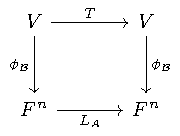
\includegraphics[width=0.3\textwidth]{figuras/diagrama-valores-propios.pdf}
    \end{figure}

    Supongamos que $v$ es vector propio de $T$ correspondiente a $\lambda$. Entonces $T(v) = \lambda v$, de donde
    \begin{equation*}
        A\phi_{\BB}(v) = L_A\phi_{\BB}(v) = \phi_{\BB}T(v) = \phi_{\BB}(\lambda v) = \lambda \phi_{\BB}(v).
    \end{equation*}
    Como $\phi_{\BB}$ es un isomorfismo, $\phi_{\BB}(v) \neq 0$; luego $\phi_{\BB}(v)$ es vector propio de $A$ correspondiente a $\lambda$. Este argumento es reversible, así que también se cumple el recíproco: si $\phi_{\BB}(v)$ es vector propio de $A$ correspondiente a $\lambda$, entonces $v$ es vector propio de $T$ correspondiente a $\lambda$.

    Una formulación equivalente de lo anterior es la siguiente: para un valor propio $\lambda$ de $A$ (y por tanto de $T$), un vector $y \in F^n$ es vector propio de $A$ correspondiente a $\lambda$ si y solo si $\phi_{\BB}^{-1}(y)$ es vector propio de $T$ correspondiente a $\lambda$.

    Hemos reducido así el problema de encontrar los vectores propios de un operador lineal sobre un espacio vectorial de dimensión finita al problema de encontrar los vectores propios de una matriz. El siguiente ejemplo ilustra este procedimiento.

    \begin{ejemplo}
        Sea $T$ el operador lineal sobre $P_2(\R)$ definido en un ejemplo anterior, y sea $\BB$ la base canónica de $P_2(\R)$. Recordemos que $T$ tiene valores propios $1$, $2$ y $3$, y que
        \begin{equation*}
            A = [T]_{\BB} = \begin{pmatrix} 1 & 1 & 0 \\ 0 & 2 & 2 \\ 0 & 0 & 3 \end{pmatrix}.
        \end{equation*}
        Consideramos cada valor propio por separado.

        Sea $\lambda_1 = 1$, y definamos
        \begin{equation*}
            B_1 = A - \lambda_1 I = \begin{pmatrix} 0 & 1 & 0 \\ 0 & 1 & 2 \\ 0 & 0 & 2 \end{pmatrix}.
        \end{equation*}
        Entonces $x = (x_1,x_2,x_3) \in \R^3$ es vector propio correspondiente a $\lambda_1 = 1$ si y solo si $x \neq 0$ y $x$ es solución del sistema
        \begin{align*}
            x_2 &= 0 \\
            x_2 + 2x_3 &= 0 \\
            2x_3 &= 0.
        \end{align*}
        Este sistema tiene tres incógnitas, $x_1, x_2, x_3$, pero $x_1$ no aparece en ninguna ecuación. Como el valor de $x_1$ no afecta al sistema, le asignamos un valor paramétrico $x_1 = a$ y resolvemos para $x_2$ y $x_3$. Claramente $x_2 = x_3 = 0$, de modo que los vectores propios de $A$ correspondientes a $\lambda_1 = 1$ son de la forma
        \begin{equation*}
            a\begin{pmatrix} 1 \\ 0 \\ 0 \end{pmatrix} = a\, e_1
        \end{equation*}
        para $a \neq 0$. En consecuencia, los vectores propios de $T$ correspondientes a $\lambda_1 = 1$ son de la forma
        \begin{equation*}
            \phi_{\BB}^{-1}(a e_1) = a\, \phi_{\BB}^{-1}(e_1) = a \cdot 1 = a
        \end{equation*}
        para cualquier $a \neq 0$. Es decir, los polinomios constantes no nulos son los vectores propios de $T$ correspondientes a $\lambda_1 = 1$.

        Sea ahora $\lambda_2 = 2$, y definamos
        \begin{equation*}
            B_2 = A - \lambda_2 I = \begin{pmatrix} -1 & 1 & 0 \\ 0 & 0 & 2 \\ 0 & 0 & 1 \end{pmatrix}.
        \end{equation*}
        Se verifica fácilmente que
        \begin{equation*}
            \ker(L_{B_2}) = \left\{ a\begin{pmatrix} 1 \\ 1 \\ 0 \end{pmatrix} : a \in \R \right\},
        \end{equation*}
        y por tanto los vectores propios de $T$ correspondientes a $\lambda_2 = 2$ son de la forma
        \begin{equation*}
            \phi_{\BB}^{-1}\left(a\begin{pmatrix} 1\\1\\0\end{pmatrix}\right) = a\, \phi_{\BB}^{-1}(e_1+e_2) = a(1+x)
        \end{equation*}
        para $a \neq 0$.

        Finalmente, consideremos $\lambda_3 = 3$ y
        \begin{equation*}
            B_3 = A - \lambda_3 I = \begin{pmatrix} -2 & 1 & 0 \\ 0 & -1 & 2 \\ 0 & 0 & 0 \end{pmatrix}.
        \end{equation*}
        Como
        \begin{equation*}
            \ker(L_{B_3}) = \left\{ a\begin{pmatrix} 1\\2\\1\end{pmatrix} : a \in \R \right\},
        \end{equation*}
        los vectores propios de $T$ correspondientes a $\lambda_3 = 3$ son de la forma
        \begin{equation*}
            \phi_{\BB}^{-1}\left(a\begin{pmatrix}1\\2\\1\end{pmatrix}\right) = a\,\phi_{\BB}^{-1}(e_1+2e_2+e_3) = a(1+2x+x^2)
        \end{equation*}
        para $a \neq 0$.

        Tomando, para cada valor propio, el vector propio correspondiente con $a=1$, obtenemos $\gamma = \{1,\, 1+x,\, 1+2x+x^2\}$, una base ordenada de $P_2(\R)$ formada por vectores propios de $T$. Así, $T$ es diagonalizable, y
        \begin{equation*}
            [T]_\gamma = \begin{pmatrix} 1 & 0 & 0 \\ 0 & 2 & 0 \\ 0 & 0 & 3 \end{pmatrix}.
        \end{equation*}
    \end{ejemplo}

    Cerramos esta sección con una descripción geométrica de cómo actúa un operador lineal $T$ sobre un vector propio, en el contexto de un espacio vectorial $V$ sobre $\R$. Sea $v$ un vector propio de $T$ y $\lambda$ el valor propio correspondiente. Podemos pensar en $W = \gen{v}$, el subespacio de $V$ de dimensión uno generado por $v$, como una recta en $V$ que pasa por $0$ y por $v$. Para cualquier $w \in W$, $w = cv$ para algún escalar $c$, y por tanto
    \begin{equation*}
        T(w) = T(cv) = cT(v) = c\lambda v = \lambda w;
    \end{equation*}
    así que $T$ actúa sobre los vectores de $W$ multiplicando cada uno por $\lambda$. Existen varias formas en que $T$ puede actuar sobre los vectores de $W$, dependiendo del valor de $\lambda$. Consideramos varios casos (véase la siguiente figura).

    \begin{enumerate}
        \item[\textbf{Caso 1.}] Si $\lambda > 1$, $T$ aleja los vectores de $W$ del origen $0$ por un factor de $\lambda$.
        \item[\textbf{Caso 2.}] Si $\lambda = 1$, $T$ actúa como la identidad sobre $W$.
        \item[\textbf{Caso 3.}] Si $0 < \lambda < 1$, $T$ acerca los vectores de $W$ al origen $0$ por un factor de $\lambda$.
        \item[\textbf{Caso 4.}] Si $\lambda = 0$, $T$ actúa como la transformación cero sobre $W$.
        \item[\textbf{Caso 5.}] Si $\lambda < 0$, $T$ invierte la orientación de $W$; es decir, $T$ manda los vectores de $W$ de un lado de $0$ al otro.
    \end{enumerate}

    \begin{figure}[H]
        \centering
        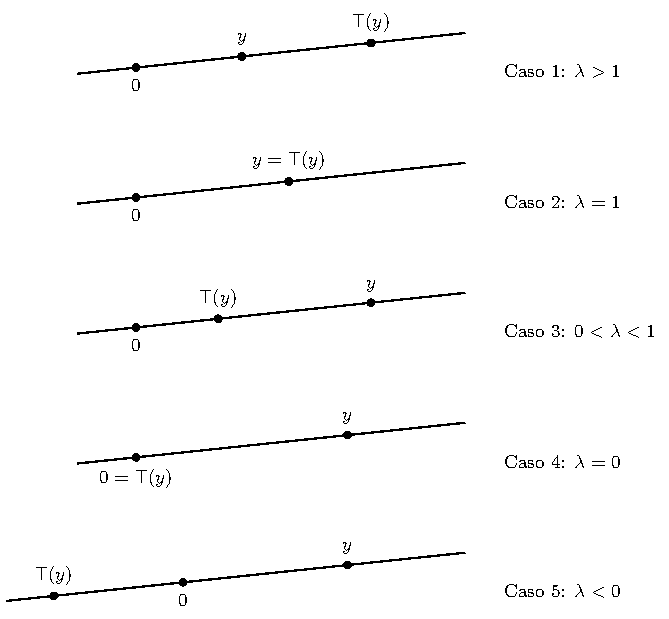
\includegraphics[width=0.55\textwidth]{figuras/accion-vector-propio.pdf}
    \end{figure}

    Para ilustrar estas ideas, consideramos los operadores lineales de los ejemplos anteriores de esta sección.

    Para el operador $T$ sobre $\R^2$ dado por $T(a_1,a_2) = (a_1,-a_2)$ (la reflexión respecto al eje $x$), $e_1$ y $e_2$ son vectores propios de $T$ con valores propios correspondientes $1$ y $-1$, respectivamente. Como $e_1$ y $e_2$ generan al eje $x$ y al eje $y$, respectivamente, $T$ actúa como la identidad sobre el eje $x$ e invierte la orientación del eje $y$.

    Para el operador $T$ sobre $\R^2$ dado por $T(a_1,a_2)=(a_1,0)$ (la proyección sobre el eje $x$), $e_1$ y $e_2$ son vectores propios de $T$ con valores propios correspondientes $1$ y $0$, respectivamente. Así, $T$ actúa como la identidad sobre el eje $x$ y como la transformación cero sobre el eje $y$.

    Por último, generalizamos el ejemplo de la rotación por $\pi/2$ considerando el operador que gira el plano un ángulo $\theta$, definido por
    \begin{equation*}
        T_\theta(a_1,a_2) = (a_1\cos\theta - a_2\sin\theta,\; a_1\sin\theta + a_2\cos\theta).
    \end{equation*}
    Supongamos que $0 < \theta < \pi$. Entonces, para cualquier vector no nulo $v$, los vectores $v$ y $T_\theta(v)$ no son colineales, así que $T_\theta$ no manda ningún subespacio de dimensión uno de $\R^2$ en sí mismo. Por tanto $T_\theta$ no tiene vectores propios y, en consecuencia, tampoco valores propios. Para confirmar esta conclusión, notemos que el polinomio característico de $T_\theta$ es
    \begin{equation*}
        \det(T_\theta - tI) = \det\begin{pmatrix} \cos\theta - t & -\sin\theta \\ \sin\theta & \cos\theta - t\end{pmatrix} = t^2 - (2\cos\theta) t + 1,
    \end{equation*}
    el cual no tiene raíces reales, pues para $0 < \theta < \pi$ el discriminante $4\cos^2\theta - 4$ es negativo.

    \section{Diagonalizabilidad}

    En la sección anterior presentamos el problema de la diagonalización y observamos que no todos los operadores lineales o matrices son diagonalizables. Aunque somos capaces de diagonalizar operadores y matrices, e incluso obtuvimos una condición necesaria y suficiente para la diagonalizabilidad (Teorema~5.1), aún no hemos resuelto el problema de la diagonalización. Lo que falta es una prueba sencilla para determinar si un operador o una matriz puede diagonalizarse, así como un método para encontrar efectivamente una base de vectores propios. En esta sección desarrollamos tal prueba y tal método.

    En el ejemplo de la sección anterior donde diagonalizamos la matriz $\begin{pmatrix}1&1\\4&1\end{pmatrix}$, obtuvimos una base de vectores propios eligiendo un vector propio correspondiente a cada valor propio. En general, este procedimiento no produce una base, pero el siguiente teorema muestra que todo conjunto construido de esta manera es linealmente independiente.

    \begin{teorema}
        Sea $T$ un operador lineal sobre un espacio vectorial $V$, y sean $\lambda_1, \lambda_2, \dots, \lambda_k$ valores propios distintos de $T$. Si $v_1, v_2, \dots, v_k$ son vectores propios de $T$ tales que $\lambda_i$ corresponde a $v_i$ ($1\le i\le k$), entonces $\{v_1,\dots,v_k\}$ es linealmente independiente.
    \end{teorema}

    \begin{proof}
        Procedemos por inducción sobre $k$. Si $k=1$, entonces $v_1\neq 0$ por ser vector propio, y por tanto $\{v_1\}$ es linealmente independiente.

        Supongamos que el teorema es válido para $k-1$ valores propios distintos, con $k-1\geq 1$, y que tenemos $k$ vectores propios $v_1,\dots,v_k$ correspondientes a los valores propios distintos $\lambda_1,\dots,\lambda_k$. Queremos mostrar que $\{v_1,\dots,v_k\}$ es linealmente independiente. Supongamos que $a_1,\dots,a_k$ son escalares tales que
        \begin{equation*}
            a_1v_1+a_2v_2+\cdots+a_kv_k=0. \tag{$*$}
        \end{equation*}
        Aplicando $T-\lambda_k I$ a ambos lados de ($*$),
        \begin{equation*}
            a_1(\lambda_1-\lambda_k)v_1+a_2(\lambda_2-\lambda_k)v_2+\cdots+a_{k-1}(\lambda_{k-1}-\lambda_k)v_{k-1}=0.
        \end{equation*}
        Por hipótesis de inducción, $\{v_1,\dots,v_{k-1}\}$ es linealmente independiente, así que
        \begin{equation*}
            a_1(\lambda_1-\lambda_k)=a_2(\lambda_2-\lambda_k)=\cdots=a_{k-1}(\lambda_{k-1}-\lambda_k)=0.
        \end{equation*}
        Como $\lambda_1,\dots,\lambda_k$ son distintos, $\lambda_i-\lambda_k\neq 0$ para $1\leq i\leq k-1$, de donde $a_1=a_2=\cdots=a_{k-1}=0$, y ($*$) se reduce a $a_kv_k=0$. Pero $v_k\neq 0$, así que $a_k=0$. En consecuencia $a_1=\cdots=a_k=0$, y $\{v_1,\dots,v_k\}$ es linealmente independiente.
    \end{proof}

    \begin{corolario}
        Sea $T$ un operador lineal sobre un espacio vectorial $V$ de dimensión $n$. Si $T$ tiene $n$ valores propios distintos, entonces $T$ es diagonalizable.
    \end{corolario}

    \begin{proof}
        Supongamos que $T$ tiene $n$ valores propios distintos $\lambda_1,\dots,\lambda_n$. Para cada $i$, elijamos un vector propio $v_i$ correspondiente a $\lambda_i$. Por el teorema anterior, $\{v_1,\dots,v_n\}$ es linealmente independiente, y como $\dim(V)=n$, este conjunto es una base de $V$. Así, por el Teorema~5.1, $T$ es diagonalizable.
    \end{proof}

    \begin{ejemplo}
        Sea
        \begin{equation*}
            A=\begin{pmatrix}1&1\\1&1\end{pmatrix}\in M_{2\times2}(\R).
        \end{equation*}
        El polinomio característico de $A$ (y por tanto de $L_A$) es
        \begin{equation*}
            \det(A-tI)=\det\begin{pmatrix}1-t&1\\1&1-t\end{pmatrix}=t(t-2),
        \end{equation*}
        así que los valores propios de $L_A$ son $0$ y $2$. Como $L_A$ es un operador lineal sobre el espacio vectorial de dimensión dos $\R^2$, concluimos por el corolario anterior que $L_A$ (y por tanto $A$) es diagonalizable.
    \end{ejemplo}

    El recíproco del teorema anterior es falso: no es cierto que, si $T$ es diagonalizable, entonces $T$ tiene $n$ valores propios distintos. Por ejemplo, el operador identidad es diagonalizable aunque tiene un único valor propio, $\lambda=1$.

    Hemos visto que la diagonalizabilidad requiere la existencia de valores propios. De hecho, la diagonalizabilidad impone una condición más fuerte sobre el polinomio característico.

    \begin{definicion}[Polinomio que se escinde]
        Un polinomio $f(t) \in P(F)$ \textbf{se escinde} sobre $F$ si existen escalares $c,a_1,\dots,a_n \in F$ (no necesariamente distintos) tales que
        \begin{equation*}
            f(t)=c(t-a_1)(t-a_2)\cdots(t-a_n).
        \end{equation*}
    \end{definicion}

    Por ejemplo, $t^2-1=(t+1)(t-1)$ se escinde sobre $\R$, pero $(t^2+1)(t-2)$ no se escinde sobre $\R$ porque $t^2+1$ no puede factorizarse como producto de factores lineales sobre $\R$. Sin embargo, $(t^2+1)(t-2)$ sí se escinde sobre $\C$, pues se factoriza como $(t+i)(t-i)(t-2)$. Si $f(t)$ es el polinomio característico de un operador lineal o de una matriz sobre un campo $F$, la afirmación de que $f(t)$ se escinde se entiende como que se escinde sobre $F$.

    \begin{teorema}
        El polinomio característico de todo operador lineal diagonalizable se escinde.
    \end{teorema}

    \begin{proof}
        Sea $T$ un operador lineal diagonalizable sobre el espacio vectorial $V$ de dimensión $n$, y sea $\BB$ una base ordenada de $V$ tal que $[T]_{\BB}=D$ es una matriz diagonal. Supongamos
        \begin{equation*}
            D=\begin{pmatrix}\lambda_1&0&\cdots&0\\0&\lambda_2&\cdots&0\\\vdots&&&\vdots\\0&0&\cdots&\lambda_n\end{pmatrix},
        \end{equation*}
        y sea $f(t)$ el polinomio característico de $T$. Entonces
        \begin{align*}
            f(t)&=\det(D-tI)\\
            &=\det\begin{pmatrix}\lambda_1-t&0&\cdots&0\\0&\lambda_2-t&\cdots&0\\\vdots&&&\vdots\\0&0&\cdots&\lambda_n-t\end{pmatrix}\\
            &=(\lambda_1-t)(\lambda_2-t)\cdots(\lambda_n-t)\\
            &=(-1)^n(t-\lambda_1)(t-\lambda_2)\cdots(t-\lambda_n).
        \end{align*}
        Por lo tanto $f(t)$ se escinde.
    \end{proof}

    De este teorema es claro que, si $T$ es un operador lineal diagonalizable sobre un espacio vectorial de dimensión $n$ que no tiene $n$ valores propios distintos, entonces el polinomio característico de $T$ debe tener ceros repetidos.

    El recíproco del teorema anterior es falso: es decir, el polinomio característico de $T$ puede escindirse sin que $T$ sea diagonalizable (véase el ejemplo que sigue a la definición de subespacio propio, más adelante en esta sección). El siguiente concepto nos ayuda a determinar cuándo un operador cuyo polinomio característico se escinde es diagonalizable.

    \begin{definicion}[Multiplicidad algebraica]
        Sea $\lambda$ un valor propio de un operador lineal o de una matriz, con polinomio característico $f(t)$. La \textbf{multiplicidad algebraica} de $\lambda$ es el mayor entero positivo $k$ tal que $(t-\lambda)^k$ es un factor de $f(t)$.
    \end{definicion}

    \begin{ejemplo}
        Sea
        \begin{equation*}
            A=\begin{pmatrix}3&1&0\\0&3&4\\0&0&4\end{pmatrix},
        \end{equation*}
        cuyo polinomio característico es $f(t)=-(t-3)^2(t-4)$. Así, $\lambda=3$ es valor propio de $A$ con multiplicidad $2$, y $\lambda=4$ es valor propio de $A$ con multiplicidad $1$.
    \end{ejemplo}

    Si $T$ es un operador lineal diagonalizable sobre un espacio vectorial $V$ de dimensión finita, entonces existe una base ordenada $\BB$ de $V$ formada por vectores propios de $T$. Sabemos, por el Teorema~5.1, que $[T]_{\BB}$ es una matriz diagonal cuyas entradas diagonales son los valores propios de $T$. Como el polinomio característico de $T$ es $\det([T]_{\BB}-tI)$, se ve fácilmente que cada valor propio de $T$ debe aparecer como entrada diagonal de $[T]_{\BB}$ exactamente tantas veces como su multiplicidad. Por tanto $\BB$ contiene tantos vectores propios (linealmente independientes) correspondientes a un valor propio dado como la multiplicidad de ese valor propio. Así, el número de vectores propios linealmente independientes correspondientes a un valor propio dado resulta de interés para determinar si un operador puede diagonalizarse. Recordando, del Teorema~5.4, que los vectores propios de $T$ correspondientes al valor propio $\lambda$ son los vectores no nulos del espacio nulo de $T-\lambda I$, estudiamos a continuación este conjunto.

    \begin{definicion}[Subespacio propio]
        Sea $T$ un operador lineal sobre un espacio vectorial $V$, y sea $\lambda$ un valor propio de $T$. Se define
        \begin{equation*}
            E_\lambda=\{x\in V: T(x)=\lambda x\}=\ker(T-\lambda I_V).
        \end{equation*}
        Al conjunto $E_\lambda$ se le llama \textbf{subespacio propio} de $T$ correspondiente al valor propio $\lambda$. Análogamente, se define el subespacio propio de una matriz cuadrada $A$ como el subespacio propio de $L_A$.
    \end{definicion}

    Claramente, $E_\lambda$ es un subespacio de $V$ que consiste del vector cero y de los vectores propios de $T$ correspondientes al valor propio $\lambda$. El número máximo de vectores propios de $T$ linealmente independientes correspondientes a $\lambda$ es, por tanto, la dimensión de $E_\lambda$. El siguiente resultado relaciona esta dimensión con la multiplicidad de $\lambda$.

    \begin{teorema}
        Sea $T$ un operador lineal sobre un espacio vectorial $V$ de dimensión finita, y sea $\lambda$ un valor propio de $T$ de multiplicidad $m$. Entonces $1\leq \dim(E_\lambda)\leq m$.
    \end{teorema}

    \begin{proof}
        Elijamos una base ordenada $\{v_1,\dots,v_p\}$ para $E_\lambda$, extendámosla a una base ordenada $\BB=\{v_1,\dots,v_p,v_{p+1},\dots,v_n\}$ de $V$, y sea $A=[T]_{\BB}$. Como $v_i$ ($1\leq i\leq p$) es vector propio de $T$ correspondiente a $\lambda$,
        \begin{equation*}
            A=\begin{pmatrix}\lambda I_p&B\\O&C\end{pmatrix}
        \end{equation*}
        para ciertas matrices $B$ y $C$. Usando que el determinante de una matriz triangular por bloques es el producto de los determinantes de los bloques diagonales, el polinomio característico de $T$ es
        \begin{align*}
            f(t)&=\det(A-tI_n)=\det\begin{pmatrix}(\lambda-t)I_p&B\\O&C-tI_{n-p}\end{pmatrix}\\
            &=\det((\lambda-t)I_p)\det(C-tI_{n-p})\\
            &=(\lambda-t)^p g(t),
        \end{align*}
        donde $g(t)$ es un polinomio. Así, $(\lambda-t)^p$ es un factor de $f(t)$, y por tanto la multiplicidad de $\lambda$ es al menos $p$, es decir, $p\leq m$. Pero $\dim(E_\lambda)=p$, así que $\dim(E_\lambda)\leq m$. Como $\lambda$ es valor propio, $E_\lambda\neq\{0\}$, de donde $p\geq 1$ y por tanto $\dim(E_\lambda)\geq 1$.
    \end{proof}

    \begin{ejemplo}
        Sea $T$ el operador lineal sobre $P_2(\R)$ definido por $T(f(x))=f'(x)$. La representación matricial de $T$ respecto a la base canónica $\BB$ de $P_2(\R)$ es
        \begin{equation*}
            [T]_{\BB}=\begin{pmatrix}0&1&0\\0&0&2\\0&0&0\end{pmatrix}.
        \end{equation*}
        En consecuencia, el polinomio característico de $T$ es
        \begin{equation*}
            \det([T]_{\BB}-tI)=\det\begin{pmatrix}-t&1&0\\0&-t&2\\0&0&-t\end{pmatrix}=-t^3.
        \end{equation*}
        Así, $T$ tiene un único valor propio, $\lambda=0$, con multiplicidad $3$. Resolviendo $T(f(x))=f'(x)=0$ vemos que $E_\lambda=\ker(T-\lambda I)=\ker(T)$ es el subespacio de $P_2(\R)$ formado por los polinomios constantes. Así, $\{1\}$ es una base de $E_\lambda$, y por tanto $\dim(E_\lambda)=1$. En consecuencia, no existe base de $P_2(\R)$ formada por vectores propios de $T$, y por tanto $T$ no es diagonalizable, aunque su polinomio característico se escinde. Esto muestra que el recíproco del Teorema~5.6 es falso.
    \end{ejemplo}

    \begin{ejemplo}
        Sea $T$ el operador lineal sobre $\R^3$ definido por
        \begin{equation*}
            T\begin{pmatrix}a_1\\a_2\\a_3\end{pmatrix}=\begin{pmatrix}4a_1+a_3\\2a_1+3a_2+2a_3\\a_1+4a_3\end{pmatrix}.
        \end{equation*}
        Determinamos el subespacio propio de $T$ correspondiente a cada valor propio. Sea $\BB$ la base canónica de $\R^3$. Entonces
        \begin{equation*}
            [T]_{\BB}=\begin{pmatrix}4&0&1\\2&3&2\\1&0&4\end{pmatrix},
        \end{equation*}
        y por tanto el polinomio característico de $T$ es
        \begin{equation*}
            \det([T]_{\BB}-tI)=\det\begin{pmatrix}4-t&0&1\\2&3-t&2\\1&0&4-t\end{pmatrix}=-(t-5)(t-3)^2.
        \end{equation*}
        Así, los valores propios de $T$ son $\lambda_1=5$ y $\lambda_2=3$, con multiplicidades $1$ y $2$, respectivamente.

        Como
        \begin{equation*}
            E_{\lambda_1}=\ker(T-\lambda_1 I)=\left\{\begin{pmatrix}x_1\\x_2\\x_3\end{pmatrix}\in\R^3: \begin{pmatrix}-1&0&1\\2&-2&2\\1&0&-1\end{pmatrix}\begin{pmatrix}x_1\\x_2\\x_3\end{pmatrix}=\begin{pmatrix}0\\0\\0\end{pmatrix}\right\},
        \end{equation*}
        $E_{\lambda_1}$ es el espacio solución del sistema
        \begin{align*}
            -x_1&&+\,x_3&=0\\
            2x_1-2x_2&&+2x_3&=0\\
            x_1&&-\,x_3&=0.
        \end{align*}
        Se verifica fácilmente que
        \begin{equation*}
            \left\{\begin{pmatrix}1\\2\\1\end{pmatrix}\right\}
        \end{equation*}
        es una base de $E_{\lambda_1}$. Por tanto $\dim(E_{\lambda_1})=1$.

        Análogamente, $E_{\lambda_2}=\ker(T-\lambda_2 I)$ es el espacio solución del sistema
        \begin{align*}
            x_1&&+\,x_3&=0\\
            2x_1&&+2x_3&=0\\
            x_1&&+\,x_3&=0.
        \end{align*}
        Como la incógnita $x_2$ no aparece en este sistema, le asignamos un valor paramétrico $x_2=s$, e introducimos otro parámetro $t$ para resolver el sistema en $x_1$ y $x_3$. La solución general del sistema es
        \begin{equation*}
            \begin{pmatrix}x_1\\x_2\\x_3\end{pmatrix}=s\begin{pmatrix}0\\1\\0\end{pmatrix}+t\begin{pmatrix}-1\\0\\1\end{pmatrix}, \quad \text{para } s,t\in\R.
        \end{equation*}
        Se sigue que
        \begin{equation*}
            \left\{\begin{pmatrix}0\\1\\0\end{pmatrix}, \begin{pmatrix}-1\\0\\1\end{pmatrix}\right\}
        \end{equation*}
        es una base de $E_{\lambda_2}$, y por tanto $\dim(E_{\lambda_2})=2$.

        En este caso, la multiplicidad de cada valor propio $\lambda_i$ es igual a la dimensión del subespacio propio correspondiente $E_{\lambda_i}$. Observemos que la unión de las dos bases recién obtenidas,
        \begin{equation*}
            \left\{\begin{pmatrix}1\\2\\1\end{pmatrix}, \begin{pmatrix}0\\1\\0\end{pmatrix}, \begin{pmatrix}-1\\0\\1\end{pmatrix}\right\},
        \end{equation*}
        es linealmente independiente y, por tanto, es una base de $\R^3$ formada por vectores propios de $T$. En consecuencia, $T$ es diagonalizable.
    \end{ejemplo}

    Los ejemplos anteriores sugieren que un operador cuyo polinomio característico se escinde es diagonalizable si y solo si, para cada valor propio, la dimensión del subespacio propio correspondiente coincide con su multiplicidad. Esto es, en efecto, cierto, como mostramos a continuación. Comenzamos con el siguiente lema, una ligera variación del Teorema~5.5.

    \begin{lema}
        Sea $T$ un operador lineal, y sean $\lambda_1,\dots,\lambda_k$ valores propios distintos de $T$. Para cada $i=1,\dots,k$, sea $v_i\in E_{\lambda_i}$, el subespacio propio correspondiente a $\lambda_i$. Si
        \begin{equation*}
            v_1+v_2+\cdots+v_k=0,
        \end{equation*}
        entonces $v_i=0$ para todo $i$.
    \end{lema}

    \begin{proof}
        Supongamos lo contrario. Renumerando si es necesario, supongamos que, para algún $1\leq m\leq k$, $v_i\neq 0$ para $1\leq i\leq m$, y $v_i=0$ para $i>m$. Entonces, para cada $i\leq m$, $v_i$ es un vector propio de $T$ correspondiente a $\lambda_i$, y
        \begin{equation*}
            v_1+v_2+\cdots+v_m=0.
        \end{equation*}
        Pero esto contradice al Teorema~5.5, que afirma que estos $v_i$ son linealmente independientes. Concluimos, por tanto, que $v_i=0$ para todo $i$.
    \end{proof}

    \begin{teorema}
        Sea $T$ un operador lineal sobre un espacio vectorial $V$, y sean $\lambda_1,\dots,\lambda_k$ valores propios distintos de $T$. Para cada $i=1,\dots,k$, sea $S_i$ un subconjunto finito y linealmente independiente del subespacio propio $E_{\lambda_i}$. Entonces $S=S_1\cup S_2\cup\cdots\cup S_k$ es un subconjunto linealmente independiente de $V$.
    \end{teorema}

    \begin{proof}
        Para cada $i$, escribamos $S_i=\{v_{i1},v_{i2},\dots,v_{in_i}\}$, de modo que $S=\{v_{ij}: 1\leq j\leq n_i,\ 1\leq i\leq k\}$. Consideremos escalares $\{a_{ij}\}$ tales que
        \begin{equation*}
            \sum_{i=1}^{k}\sum_{j=1}^{n_i}a_{ij}v_{ij}=0.
        \end{equation*}
        Para cada $i$, sea
        \begin{equation*}
            w_i=\sum_{j=1}^{n_i}a_{ij}v_{ij}.
        \end{equation*}
        Entonces $w_i\in E_{\lambda_i}$ para cada $i$, y $w_1+\cdots+w_k=0$. Por el lema anterior, $w_i=0$ para todo $i$. Pero cada $S_i$ es linealmente independiente, así que $a_{ij}=0$ para todos $i,j$. Concluimos que $S$ es linealmente independiente.
    \end{proof}

    El teorema anterior nos indica cómo construir un conjunto linealmente independiente de vectores propios: basta reunir bases de cada uno de los subespacios propios. El siguiente teorema nos dice cuándo el conjunto resultante es una base de todo el espacio.

    \begin{teorema}
        Sea $T$ un operador lineal sobre un espacio vectorial $V$ de dimensión finita tal que el polinomio característico de $T$ se escinde. Sean $\lambda_1,\dots,\lambda_k$ los valores propios distintos de $T$. Entonces:
        \begin{enumerate}[label=(\alph*)]
            \item $T$ es diagonalizable si y solo si la multiplicidad de $\lambda_i$ es igual a $\dim(E_{\lambda_i})$ para todo $i$.
            \item Si $T$ es diagonalizable y $\mathcal{G}_i$ es una base ordenada de $E_{\lambda_i}$ para cada $i$, entonces $\mathcal{G}=\mathcal{G}_1\cup\mathcal{G}_2\cup\cdots\cup\mathcal{G}_k$ es una base ordenada de $V$ formada por vectores propios de $T$.
        \end{enumerate}
    \end{teorema}

    \begin{proof}
        Para cada $i$, sea $m_i$ la multiplicidad de $\lambda_i$, $d_i=\dim(E_{\lambda_i})$, y $n=\dim(V)$.

        Supongamos primero que $T$ es diagonalizable. Sea $\BB$ una base de $V$ formada por vectores propios de $T$. Para cada $i$, sea $\BB_i=\BB\cap E_{\lambda_i}$ el conjunto de vectores de $\BB$ que son vectores propios correspondientes a $\lambda_i$, y sea $n_i$ el número de vectores en $\BB_i$. Entonces $n_i\leq d_i$ para cada $i$, pues $\BB_i$ es un subconjunto linealmente independiente de un subespacio de dimensión $d_i$; y $d_i\leq m_i$ por el Teorema~5.7. Los $n_i$ suman $n$ porque $\BB$ tiene $n$ vectores; los $m_i$ también suman $n$, pues el grado del polinomio característico de $T$ es igual a la suma de las multiplicidades de los valores propios. Así,
        \begin{equation*}
            n=\sum_{i=1}^{k}n_i\leq\sum_{i=1}^{k}d_i\leq\sum_{i=1}^{k}m_i=n.
        \end{equation*}
        Se sigue que $\sum_{i=1}^{k}(m_i-d_i)=0$. Como $(m_i-d_i)\geq 0$ para todo $i$, concluimos que $m_i=d_i$ para todo $i$.

        Recíprocamente, supongamos que $m_i=d_i$ para todo $i$; probamos simultáneamente que $T$ es diagonalizable y (b). Para cada $i$, sea $\mathcal{G}_i$ una base ordenada de $E_{\lambda_i}$, y sea $\mathcal{G}=\mathcal{G}_1\cup\cdots\cup\mathcal{G}_k$. Por el Teorema~5.8, $\mathcal{G}$ es linealmente independiente. Más aún, como $d_i=m_i$ para todo $i$, $\mathcal{G}$ contiene
        \begin{equation*}
            \sum_{i=1}^{k}d_i=\sum_{i=1}^{k}m_i=n
        \end{equation*}
        vectores. Por lo tanto $\mathcal{G}$ es una base ordenada de $V$ formada por vectores propios de $T$, y concluimos que $T$ es diagonalizable.
    \end{proof}

    Este teorema completa nuestro estudio del problema de diagonalización. Resumimos nuestros resultados.

    \subsection*{Prueba para la diagonalización}

    Sea $T$ un operador lineal sobre un espacio vectorial $V$ de dimensión $n$. Entonces $T$ es diagonalizable si y solo si se cumplen las siguientes dos condiciones:
    \begin{enumerate}
        \item El polinomio característico de $T$ se escinde.
        \item Para cada valor propio $\lambda$ de $T$, la multiplicidad de $\lambda$ es igual a $n-\rg(T-\lambda I)$.
    \end{enumerate}

    Estas mismas condiciones pueden usarse para probar si una matriz cuadrada $A$ es diagonalizable, pues la diagonalizabilidad de $A$ equivale a la de $L_A$.

    Si $T$ es un operador diagonalizable y $\mathcal{G}_1,\dots,\mathcal{G}_k$ son bases ordenadas de los subespacios propios de $T$, entonces la unión $\BB=\mathcal{G}_1\cup\cdots\cup\mathcal{G}_k$ es una base ordenada de $V$ formada por vectores propios de $T$, y por tanto $[T]_{\BB}$ es diagonal.

    Al probar si $T$ es diagonalizable, suele ser más sencillo elegir una base conveniente $\mathcal{A}$ para $V$ y trabajar con $B=[T]_{\mathcal{A}}$. Si el polinomio característico de $B$ se escinde, se usa entonces la condición 2 anterior para verificar si la multiplicidad de cada valor propio \textit{repetido} de $B$ coincide con $n-\rg(B-\lambda I)$. (Por el Teorema~5.7, la condición 2 se cumple automáticamente para los valores propios de multiplicidad uno.) Si esto ocurre, entonces $B$, y por tanto $T$, es diagonalizable.

    Si $T$ es diagonalizable y se desea una base $\BB$ de $V$ formada por vectores propios de $T$, se encuentra primero una base para cada subespacio propio de $B$. La unión de estas bases es una base $\mathcal{G}$ de $F^n$ formada por vectores propios de $B$. Cada vector de $\mathcal{G}$ es el vector de coordenadas, respecto a $\mathcal{A}$, de un vector propio de $T$. El conjunto formado por estos $n$ vectores propios de $T$ es la base $\BB$ buscada.

    Más aún, si $A$ es una matriz diagonalizable de tamaño $n\times n$, podemos usar el hecho de que si $Q$ es la matriz cuyas columnas son los vectores de una base de $F^n$ formada por vectores propios de $A$, entonces $Q$ es invertible y $D=Q^{-1}AQ$ es diagonal, con entradas diagonales los valores propios de $A$ correspondientes a las columnas de $Q$.

    A continuación consideramos algunos ejemplos que ilustran las ideas anteriores.

    \begin{ejemplo}
        Probamos la diagonalizabilidad de la matriz
        \begin{equation*}
            A=\begin{pmatrix}3&1&0\\0&3&0\\0&0&4\end{pmatrix}\in M_{3\times 3}(\R).
        \end{equation*}
        El polinomio característico de $A$ es $\det(A-tI)=-(t-4)(t-3)^2$, el cual se escinde, así que se satisface la condición 1 de la prueba de diagonalización. Además $A$ tiene valores propios $\lambda_1=4$ y $\lambda_2=3$, con multiplicidades $1$ y $2$, respectivamente. Como $\lambda_1$ tiene multiplicidad $1$, la condición 2 se satisface para $\lambda_1$. Basta entonces verificar la condición 2 para $\lambda_2$. Como
        \begin{equation*}
            A-\lambda_2 I=\begin{pmatrix}0&1&0\\0&0&0\\0&0&1\end{pmatrix}
        \end{equation*}
        tiene rango $2$, se tiene $3-\rg(A-\lambda_2 I)=1$, lo cual no coincide con la multiplicidad de $\lambda_2$. Por tanto la condición 2 falla para $\lambda_2$, y $A$ no es diagonalizable.
    \end{ejemplo}

    \begin{ejemplo}
        Sea $T$ el operador lineal sobre $P_2(\R)$ definido por
        \begin{equation*}
            T(f(x))=f(1)+f'(0)x+(f'(0)+f''(0))x^2.
        \end{equation*}
        Probamos primero si $T$ es diagonalizable. Sea $\mathcal{A}$ la base canónica de $P_2(\R)$, y sea $B=[T]_{\mathcal{A}}$. Entonces
        \begin{equation*}
            B=\begin{pmatrix}1&1&1\\0&1&0\\0&1&2\end{pmatrix}.
        \end{equation*}
        El polinomio característico de $B$, y por tanto de $T$, es $-(t-1)^2(t-2)$, el cual se escinde. Así, $B$ tiene valores propios $\lambda_1=1$ y $\lambda_2=2$, con multiplicidades $2$ y $1$, respectivamente. La condición 2 se satisface para $\lambda_2$ porque tiene multiplicidad $1$. Basta entonces verificar la condición 2 para $\lambda_1=1$. Para esto,
        \begin{equation*}
            3-\rg(B-\lambda_1 I)=3-\rg\begin{pmatrix}0&1&1\\0&0&0\\0&1&1\end{pmatrix}=3-1=2,
        \end{equation*}
        que coincide con la multiplicidad de $\lambda_1$. Por lo tanto, $T$ es diagonalizable.

        Encontramos ahora una base ordenada $\mathcal{G}$ de $\R^3$ formada por vectores propios de $B$. Consideramos cada valor propio por separado.

        El subespacio propio correspondiente a $\lambda_1=1$ es
        \begin{equation*}
            E_{\lambda_1}=\left\{\begin{pmatrix}x_1\\x_2\\x_3\end{pmatrix}\in\R^3: \begin{pmatrix}0&1&1\\0&0&0\\0&1&1\end{pmatrix}\begin{pmatrix}x_1\\x_2\\x_3\end{pmatrix}=0\right\},
        \end{equation*}
        el cual es el espacio solución del sistema $x_2+x_3=0$, y tiene como base
        \begin{equation*}
            \mathcal{G}_1=\left\{\begin{pmatrix}1\\0\\0\end{pmatrix}, \begin{pmatrix}0\\-1\\1\end{pmatrix}\right\}.
        \end{equation*}

        El subespacio propio correspondiente a $\lambda_2=2$ es
        \begin{equation*}
            E_{\lambda_2}=\left\{\begin{pmatrix}x_1\\x_2\\x_3\end{pmatrix}\in\R^3: \begin{pmatrix}-1&1&1\\0&-1&0\\0&1&0\end{pmatrix}\begin{pmatrix}x_1\\x_2\\x_3\end{pmatrix}=0\right\},
        \end{equation*}
        el espacio solución del sistema $-x_1+x_2+x_3=0,\ x_2=0$, con base
        \begin{equation*}
            \mathcal{G}_2=\left\{\begin{pmatrix}1\\0\\1\end{pmatrix}\right\}.
        \end{equation*}

        Sea
        \begin{equation*}
            \mathcal{G}=\mathcal{G}_1\cup\mathcal{G}_2=\left\{\begin{pmatrix}1\\0\\0\end{pmatrix}, \begin{pmatrix}0\\-1\\1\end{pmatrix}, \begin{pmatrix}1\\0\\1\end{pmatrix}\right\}.
        \end{equation*}
        Entonces $\mathcal{G}$ es una base ordenada de $\R^3$ formada por vectores propios de $B$.

        Finalmente, observamos que los vectores de $\mathcal{G}$ son los vectores de coordenadas, respecto a $\mathcal{A}$, de los vectores del conjunto
        \begin{equation*}
            \BB=\{1,\ -x+x^2,\ 1+x^2\},
        \end{equation*}
        que es una base ordenada de $P_2(\R)$ formada por vectores propios de $T$. Así,
        \begin{equation*}
            [T]_{\BB}=\begin{pmatrix}1&0&0\\0&1&0\\0&0&2\end{pmatrix}.
        \end{equation*}
    \end{ejemplo}

    El siguiente ejemplo es una aplicación de la diagonalización.

    \begin{ejemplo}
        Sea
        \begin{equation*}
            A=\begin{pmatrix}0&-2\\1&3\end{pmatrix}.
        \end{equation*}
        Mostramos que $A$ es diagonalizable y encontramos una matriz $Q$ de tamaño $2\times2$ tal que $Q^{-1}AQ$ sea diagonal. Después mostramos cómo usar este resultado para calcular $A^n$ para cualquier entero positivo $n$.

        El polinomio característico de $A$ es $(t-1)(t-2)$, así que $A$ tiene dos valores propios distintos, $\lambda_1=1$ y $\lambda_2=2$. Aplicando el corolario al Teorema~5.5 al operador $L_A$, vemos que $A$ es diagonalizable. Más aún,
        \begin{equation*}
            \mathcal{G}_1=\left\{\begin{pmatrix}-2\\1\end{pmatrix}\right\}
            \quad\text{y}\quad
            \mathcal{G}_2=\left\{\begin{pmatrix}-1\\1\end{pmatrix}\right\}
        \end{equation*}
        son bases de los subespacios propios $E_{\lambda_1}$ y $E_{\lambda_2}$, respectivamente. Por tanto
        \begin{equation*}
            \mathcal{G}=\mathcal{G}_1\cup\mathcal{G}_2=\left\{\begin{pmatrix}-2\\1\end{pmatrix}, \begin{pmatrix}-1\\1\end{pmatrix}\right\}
        \end{equation*}
        es una base ordenada de $\R^2$ formada por vectores propios de $A$. Sea
        \begin{equation*}
            Q=\begin{pmatrix}-2&-1\\1&1\end{pmatrix}
        \end{equation*}
        la matriz cuyas columnas son los vectores de $\mathcal{G}$. Entonces, por el hecho enunciado al inicio de esta subsección,
        \begin{equation*}
            D=Q^{-1}AQ=[L_A]_{\mathcal{G}}=\begin{pmatrix}1&0\\0&2\end{pmatrix}.
        \end{equation*}

        Para encontrar $A^n$, con $n$ un entero positivo cualquiera, observemos que $A=QDQ^{-1}$. Por tanto
        \begin{align*}
            A^n&=(QDQ^{-1})^n\\
            &=(QDQ^{-1})(QDQ^{-1})\cdots(QDQ^{-1})\\
            &=QD^nQ^{-1}\\
            &=Q\begin{pmatrix}1^n&0\\0&2^n\end{pmatrix}Q^{-1}\\
            &=\begin{pmatrix}-2&-1\\1&1\end{pmatrix}\begin{pmatrix}1&0\\0&2^n\end{pmatrix}\begin{pmatrix}-1&-1\\1&2\end{pmatrix}\\
            &=\begin{pmatrix}2-2^n&2-2^{n+1}\\-1+2^n&-1+2^{n+1}\end{pmatrix}.
        \end{align*}
    \end{ejemplo}

    \subsection*{Sistemas de ecuaciones diferenciales}

    Consideremos el sistema de ecuaciones diferenciales
    \begin{align*}
        x_1'&=3x_1+x_2+x_3\\
        x_2'&=2x_1+4x_2+2x_3\\
        x_3'&=-x_1-x_2+x_3,
    \end{align*}
    donde, para cada $i$, $x_i=x_i(t)$ es una función real diferenciable de la variable real $t$. Claramente este sistema tiene una solución, a saber, aquella en la que cada $x_i(t)$ es la función cero. Determinamos todas las soluciones de este sistema.

    Sea $x:\R\to\R^3$ la función definida por
    \begin{equation*}
        x(t)=\begin{pmatrix}x_1(t)\\x_2(t)\\x_3(t)\end{pmatrix}.
    \end{equation*}
    La \textbf{derivada} de $x$, denotada $x'$, se define por
    \begin{equation*}
        x'(t)=\begin{pmatrix}x_1'(t)\\x_2'(t)\\x_3'(t)\end{pmatrix}.
    \end{equation*}
    Sea
    \begin{equation*}
        A=\begin{pmatrix}3&1&1\\2&4&2\\-1&-1&1\end{pmatrix}
    \end{equation*}
    la matriz de coeficientes del sistema dado, de modo que podemos reescribir el sistema como la ecuación matricial $x'=Ax$.

    Se puede verificar que, para
    \begin{equation*}
        Q=\begin{pmatrix}-1&0&-1\\0&-1&-2\\1&1&1\end{pmatrix}
        \quad\text{y}\quad
        D=\begin{pmatrix}2&0&0\\0&2&0\\0&0&4\end{pmatrix},
    \end{equation*}
    se tiene $Q^{-1}AQ=D$. Sustituyendo $A=QDQ^{-1}$ en $x'=Ax$ obtenemos $x'=QDQ^{-1}x$, o equivalentemente, $Q^{-1}x'=DQ^{-1}x$. La función $y:\R\to\R^3$ definida por $y(t)=Q^{-1}x(t)$ es diferenciable, y $y'=Q^{-1}x'$. Así, el sistema original puede escribirse como $y'=Dy$.

    Como $D$ es una matriz diagonal, el sistema $y'=Dy$ es fácil de resolver. Escribiendo
    \begin{equation*}
        y(t)=\begin{pmatrix}y_1(t)\\y_2(t)\\y_3(t)\end{pmatrix},
    \end{equation*}
    podemos reescribir $y'=Dy$ como
    \begin{equation*}
        \begin{pmatrix}y_1'(t)\\y_2'(t)\\y_3'(t)\end{pmatrix}=\begin{pmatrix}2&0&0\\0&2&0\\0&0&4\end{pmatrix}\begin{pmatrix}y_1(t)\\y_2(t)\\y_3(t)\end{pmatrix}=\begin{pmatrix}2y_1(t)\\2y_2(t)\\4y_3(t)\end{pmatrix}.
    \end{equation*}
    Las tres ecuaciones
    \begin{align*}
        y_1'&=2y_1\\
        y_2'&=2y_2\\
        y_3'&=4y_3
    \end{align*}
    son independientes entre sí, y por tanto pueden resolverse por separado. Como vimos en un ejemplo de la sección anterior, la solución general de estas ecuaciones es $y_1(t)=c_1e^{2t}$, $y_2(t)=c_2e^{2t}$ y $y_3(t)=c_3e^{4t}$, donde $c_1,c_2,c_3$ son constantes arbitrarias. Finalmente,
    \begin{align*}
        \begin{pmatrix}x_1(t)\\x_2(t)\\x_3(t)\end{pmatrix}=x(t)=Qy(t)&=\begin{pmatrix}-1&0&-1\\0&-1&-2\\1&1&1\end{pmatrix}\begin{pmatrix}c_1e^{2t}\\c_2e^{2t}\\c_3e^{4t}\end{pmatrix}\\
        &=\begin{pmatrix}-c_1e^{2t}-c_3e^{4t}\\-c_2e^{2t}-2c_3e^{4t}\\c_1e^{2t}+c_2e^{2t}+c_3e^{4t}\end{pmatrix}
    \end{align*}
    nos da la solución general del sistema original. Observemos que esta solución puede escribirse como
    \begin{equation*}
        x(t)=e^{2t}\left[c_1\begin{pmatrix}-1\\0\\1\end{pmatrix}+c_2\begin{pmatrix}0\\-1\\1\end{pmatrix}\right]+e^{4t}\left[c_3\begin{pmatrix}-1\\-2\\1\end{pmatrix}\right].
    \end{equation*}
    Las expresiones entre corchetes son vectores arbitrarios de $E_{\lambda_1}$ y $E_{\lambda_2}$, respectivamente, donde $\lambda_1=2$ y $\lambda_2=4$. Así, la solución general del sistema original es $x(t)=e^{2t}z_1+e^{4t}z_2$, donde $z_1\in E_{\lambda_1}$ y $z_2\in E_{\lambda_2}$.

    \subsection*{Sumas directas}

    Sea $T$ un operador lineal sobre un espacio vectorial $V$ de dimensión finita. Existe una manera de descomponer $V$ en subespacios más simples que ofrece información sobre el comportamiento de $T$. Este enfoque es especialmente útil para operadores no diagonalizables. En el caso de operadores diagonalizables, los subespacios más simples son los subespacios propios del operador.

    \begin{definicion}[Suma de subespacios]
        Sean $W_1,W_2,\dots,W_k$ subespacios de un espacio vectorial $V$. Se define la \textbf{suma} de estos subespacios como el conjunto
        \begin{equation*}
            \{v_1+v_2+\cdots+v_k: v_i\in W_i \text{ para } 1\leq i\leq k\},
        \end{equation*}
        el cual se denota por $W_1+W_2+\cdots+W_k$ o $\sum_{i=1}^{k}W_i$.
    \end{definicion}

    No es difícil verificar que la suma de subespacios de un espacio vectorial es también un subespacio.

    \begin{ejemplo}
        Sea $V=\R^3$, sea $W_1$ el plano $xy$, y sea $W_2$ el plano $yz$. Entonces $\R^3=W_1+W_2$, pues para cualquier vector $(a,b,c)\in\R^3$,
        \begin{equation*}
            (a,b,c)=(a,0,0)+(0,b,c),
        \end{equation*}
        donde $(a,0,0)\in W_1$ y $(0,b,c)\in W_2$.
    \end{ejemplo}

    Observemos que, en el ejemplo anterior, la representación de $(a,b,c)$ como suma de vectores de $W_1$ y $W_2$ no es única. Por ejemplo, $(a,b,c)=(a,b,0)+(0,0,c)$ es otra representación. Como con frecuencia nos interesan las sumas para las cuales estas representaciones son únicas, introducimos una condición que garantiza esta propiedad.

    \begin{definicion}[Suma directa]
        Sean $W_1,W_2,\dots,W_k$ subespacios de un espacio vectorial $V$. Decimos que $V$ es la \textbf{suma directa} de los subespacios $W_1,\dots,W_k$, y escribimos $V=W_1\oplus W_2\oplus\cdots\oplus W_k$, si
        \begin{equation*}
            V=\sum_{i=1}^{k}W_i
        \end{equation*}
        y
        \begin{equation*}
            W_j\cap\sum_{i\neq j}W_i=\{0\}\quad\text{para cada } j\ (1\leq j\leq k).
        \end{equation*}
    \end{definicion}

    \begin{ejemplo}
        Sea $V=\R^4$, $W_1=\{(a,b,0,0): a,b\in\R\}$, $W_2=\{(0,0,c,0): c\in\R\}$, y $W_3=\{(0,0,0,d): d\in\R\}$. Para cualquier $(a,b,c,d)\in V$,
        \begin{equation*}
            (a,b,c,d)=(a,b,0,0)+(0,0,c,0)+(0,0,0,d)\in W_1+W_2+W_3.
        \end{equation*}
        Así,
        \begin{equation*}
            V=\sum_{i=1}^{3}W_i.
        \end{equation*}
        Para mostrar que $V$ es la suma directa de $W_1,W_2$ y $W_3$, debemos probar que
        \begin{equation*}
            W_1\cap(W_2+W_3)=W_2\cap(W_1+W_3)=W_3\cap(W_1+W_2)=\{0\}.
        \end{equation*}
        Pero estas igualdades son evidentes, así que $V=W_1\oplus W_2\oplus W_3$.
    \end{ejemplo}

    \begin{teorema}
        Sean $W_1,\dots,W_k$ subespacios de un espacio vectorial $V$ de dimensión finita. Las siguientes condiciones son equivalentes:
        \begin{enumerate}[label=(\alph*)]
            \item $V=W_1\oplus W_2\oplus\cdots\oplus W_k$.
            \item $V=\sum_{i=1}^{k}W_i$, y para cualesquiera vectores $v_1,\dots,v_k$ con $v_i\in W_i$ ($1\leq i\leq k$), si $v_1+\cdots+v_k=0$, entonces $v_i=0$ para todo $i$.
            \item Todo vector $v\in V$ puede escribirse de manera única como $v=v_1+\cdots+v_k$, con $v_i\in W_i$.
            \item Si $\mathcal{G}_i$ es una base ordenada de $W_i$ ($1\leq i\leq k$), entonces $\mathcal{G}_1\cup\mathcal{G}_2\cup\cdots\cup\mathcal{G}_k$ es una base ordenada de $V$.
            \item Para cada $i=1,\dots,k$, existe una base ordenada $\mathcal{G}_i$ de $W_i$ tal que $\mathcal{G}_1\cup\mathcal{G}_2\cup\cdots\cup\mathcal{G}_k$ es una base ordenada de $V$.
        \end{enumerate}
    \end{teorema}

    \begin{proof}
        Probamos que (a)$\Rightarrow$(b)$\Rightarrow$(c)$\Rightarrow$(d)$\Rightarrow$(e)$\Rightarrow$(a).

        \textbf{(a) $\Rightarrow$ (b).} Supongamos (a). Claramente $V=\sum_{i=1}^{k}W_i$. Sean $v_1,\dots,v_k$ vectores tales que $v_i\in W_i$ para todo $i$ y $v_1+\cdots+v_k=0$. Para cualquier $j$,
        \begin{equation*}
            -v_j=\sum_{i\neq j}v_i\in\sum_{i\neq j}W_i.
        \end{equation*}
        Pero $-v_j\in W_j$, así que
        \begin{equation*}
            -v_j\in W_j\cap\sum_{i\neq j}W_i=\{0\}.
        \end{equation*}
        Por tanto $v_j=0$, probando (b).

        \textbf{(b) $\Rightarrow$ (c).} Supongamos (b), y sea $v\in V$. Por (b), existen vectores $v_1,\dots,v_k$ con $v_i\in W_i$ tales que $v=v_1+\cdots+v_k$. Debemos mostrar que esta representación es única. Supongamos también que $v=w_1+\cdots+w_k$, con $w_i\in W_i$ para todo $i$. Entonces
        \begin{equation*}
            (v_1-w_1)+(v_2-w_2)+\cdots+(v_k-w_k)=0,
        \end{equation*}
        y como $v_i-w_i\in W_i$ para todo $i$, (b) implica que $v_i-w_i=0$ para todo $i$. Así $v_i=w_i$ para todo $i$, probando la unicidad de la representación.

        \textbf{(c) $\Rightarrow$ (d).} Supongamos (c). Para cada $i$, sea $\mathcal{G}_i$ una base ordenada de $W_i$. Como $V=\sum_{i=1}^{k}W_i$ por (c), se sigue que $\mathcal{G}_1\cup\cdots\cup\mathcal{G}_k$ genera a $V$. Para mostrar que este conjunto es linealmente independiente, consideremos vectores $v_{ij}\in\mathcal{G}_i$ ($j=1,\dots,m_i$; $i=1,\dots,k$) y escalares $a_{ij}$ tales que
        \begin{equation*}
            \sum_{i,j}a_{ij}v_{ij}=0.
        \end{equation*}
        Para cada $i$, sea
        \begin{equation*}
            w_i=\sum_{j=1}^{m_i}a_{ij}v_{ij}.
        \end{equation*}
        Entonces, para cada $i$, $w_i\in\gen{\mathcal{G}_i}=W_i$, y
        \begin{equation*}
            w_1+w_2+\cdots+w_k=\sum_{i,j}a_{ij}v_{ij}=0.
        \end{equation*}
        Como $0\in W_i$ para cada $i$, y $0+0+\cdots+0=w_1+\cdots+w_k$, (c) implica que $w_i=0$ para todo $i$. Así,
        \begin{equation*}
            0=w_i=\sum_{j=1}^{m_i}a_{ij}v_{ij}
        \end{equation*}
        para cada $i$. Pero cada $\mathcal{G}_i$ es linealmente independiente, así que $a_{ij}=0$ para todos $i,j$. En consecuencia $\mathcal{G}_1\cup\cdots\cup\mathcal{G}_k$ es linealmente independiente y, por tanto, es una base de $V$.

        \textbf{(d) $\Rightarrow$ (e).} Es inmediato de (d).

        \textbf{(e) $\Rightarrow$ (a).} Finalmente, supongamos (e). Para cada $i$, sea $\mathcal{G}_i$ una base ordenada de $W_i$ tal que $\mathcal{G}_1\cup\cdots\cup\mathcal{G}_k$ es una base ordenada de $V$. Entonces
        \begin{align*}
            V&=\gen{\mathcal{G}_1\cup\cdots\cup\mathcal{G}_k}\\
            &=\gen{\mathcal{G}_1}+\cdots+\gen{\mathcal{G}_k}=\sum_{i=1}^{k}W_i,
        \end{align*}
        pues el generado de una unión de conjuntos es la suma de sus generados. Fijemos $j$ ($1\leq j\leq k$), y supongamos que, para algún vector no nulo $v\in V$,
        \begin{equation*}
            v\in W_j\cap\sum_{i\neq j}W_i.
        \end{equation*}
        Entonces
        \begin{equation*}
            v\in W_j=\gen{\mathcal{G}_j}
            \quad\text{y}\quad
            v\in\sum_{i\neq j}W_i=\gen{\textstyle\bigcup_{i\neq j}\mathcal{G}_i}.
        \end{equation*}
        Así, $v$ es una combinación lineal no trivial tanto de $\mathcal{G}_j$ como de $\bigcup_{i\neq j}\mathcal{G}_i$, de modo que $v$ puede expresarse como combinación lineal de $\mathcal{G}_1\cup\cdots\cup\mathcal{G}_k$ de más de una manera. Pero esto contradice la independencia lineal de $\mathcal{G}_1\cup\cdots\cup\mathcal{G}_k$, pues en un conjunto linealmente independiente todo vector de su generado se escribe de manera única como combinación lineal de sus elementos. Concluimos que
        \begin{equation*}
            W_j\cap\sum_{i\neq j}W_i=\{0\},
        \end{equation*}
        lo cual prueba (a).
    \end{proof}

    \begin{teorema}
        Un operador lineal $T$ sobre un espacio vectorial $V$ de dimensión finita es diagonalizable si y solo si $V$ es la suma directa de los subespacios propios de $T$.
    \end{teorema}

    \begin{proof}
        Sean $\lambda_1,\dots,\lambda_k$ los valores propios distintos de $T$.

        Supongamos primero que $T$ es diagonalizable, y para cada $i$ elijamos una base ordenada $\mathcal{G}_i$ del subespacio propio $E_{\lambda_i}$. Por el Teorema~5.9, $\mathcal{G}_1\cup\cdots\cup\mathcal{G}_k$ es una base de $V$, y por tanto, por el teorema anterior, $V$ es la suma directa de los $E_{\lambda_i}$.

        Recíprocamente, supongamos que $V$ es la suma directa de los subespacios propios de $T$. Para cada $i$, elijamos una base ordenada $\mathcal{G}_i$ de $E_{\lambda_i}$. Por el teorema anterior, la unión $\mathcal{G}_1\cup\cdots\cup\mathcal{G}_k$ es una base de $V$. Como esta base está formada por vectores propios de $T$, concluimos que $T$ es diagonalizable.
    \end{proof}

    \begin{ejemplo}
        Sea $T$ el operador lineal sobre $\R^4$ definido por
        \begin{equation*}
            T(a,b,c,d)=(a,b,2c,3d).
        \end{equation*}
        Se verifica fácilmente que $T$ es diagonalizable, con valores propios $\lambda_1=1$, $\lambda_2=2$ y $\lambda_3=3$. Más aún, los subespacios propios correspondientes coinciden con los subespacios $W_1,W_2,W_3$ de un ejemplo anterior. Así, el teorema anterior nos da otra prueba de que $\R^4=W_1\oplus W_2\oplus W_3$.
    \end{ejemplo}

    \section{Límites de matrices y cadenas de Markov}

    En esta sección aplicamos lo que hemos aprendido en este capítulo para estudiar el \textit{límite} de una sucesión de potencias $A,A^2,\dots,A^n,\dots$, donde $A$ es una matriz cuadrada con entradas complejas. Estas sucesiones, y sus límites, tienen aplicaciones prácticas en las ciencias naturales y sociales.

    Suponemos familiaridad con los límites de sucesiones de números reales. El límite de una sucesión de números complejos $\{z_m:m=1,2,\dots\}$ puede definirse en términos de los límites de las sucesiones de sus partes real e imaginaria: si $z_m=r_m+is_m$, donde $r_m$ y $s_m$ son números reales, e $i$ es el número imaginario tal que $i^2=-1$, entonces
    \begin{equation*}
        \lim_{m\to\infty} z_m=\lim_{m\to\infty}r_m+i\lim_{m\to\infty}s_m,
    \end{equation*}
    siempre que $\lim_{m\to\infty}r_m$ y $\lim_{m\to\infty}s_m$ existan.

    \begin{definicion}[Límite de una sucesión de matrices]
        Sean $L,A_1,A_2,\dots$ matrices de tamaño $n\times p$ con entradas complejas. Se dice que la sucesión $A_1,A_2,\dots$ \textbf{converge} a la matriz $L$, llamada el \textbf{límite} de la sucesión, si
        \begin{equation*}
            \lim_{m\to\infty}(A_m)_{ij}=L_{ij}
        \end{equation*}
        para todo $1\leq i\leq n$ y $1\leq j\leq p$. Para indicar que $L$ es el límite de la sucesión, escribimos
        \begin{equation*}
            \lim_{m\to\infty}A_m=L.
        \end{equation*}
    \end{definicion}

    \begin{ejemplo}
        Si
        \begin{equation*}
            A_m=\begin{pmatrix}
                1-\dfrac1m & \left(-\dfrac34\right)^{m} & \dfrac{3m^2}{m^2+1}+i\left(\dfrac{2m+1}{m-1}\right) \\[2ex]
                \left(\dfrac{i}{2}\right)^{m} & 2 & \left(1+\dfrac1m\right)^{m}
            \end{pmatrix},
        \end{equation*}
        entonces
        \begin{equation*}
            \lim_{m\to\infty}A_m=\begin{pmatrix}1&0&3+2i\\0&2&e\end{pmatrix},
        \end{equation*}
        donde $e$ es la base del logaritmo natural.
    \end{ejemplo}

    Una propiedad sencilla, pero importante, de los límites de matrices está contenida en el siguiente teorema. Obsérvese la analogía con la propiedad familiar de los límites de sucesiones de números reales que afirma que, si $\lim_{m\to\infty}a_m$ existe, entonces $\lim_{m\to\infty}ca_m=c\left(\lim_{m\to\infty}a_m\right)$.

    \begin{teorema}
        Sea $A_1,A_2,\dots$ una sucesión de matrices $n\times p$ con entradas complejas que converge a la matriz $L$. Entonces, para cualesquiera $P\in M_{r\times n}(\C)$ y $Q\in M_{p\times s}(\C)$,
        \begin{equation*}
            \lim_{m\to\infty}PA_m=PL \qquad\text{y}\qquad \lim_{m\to\infty}A_mQ=LQ.
        \end{equation*}
    \end{teorema}

    \begin{proof}
        Para cualesquiera $i$ ($1\leq i\leq r$) y $j$ ($1\leq j\leq p$),
        \begin{align*}
            \lim_{m\to\infty}(PA_m)_{ij}&=\lim_{m\to\infty}\sum_{k=1}^{n}P_{ik}(A_m)_{kj}
            =\sum_{k=1}^{n}P_{ik}\cdot\lim_{m\to\infty}(A_m)_{kj}=\sum_{k=1}^{n}P_{ik}L_{kj}=(PL)_{ij}.
        \end{align*}
        Por tanto $\lim_{m\to\infty}PA_m=PL$. La demostración de que $\lim_{m\to\infty}A_mQ=LQ$ es análoga.
    \end{proof}

    \begin{corolario}
        Sea $A\in M_{n\times n}(\C)$ tal que $\lim_{m\to\infty}A^m=L$. Entonces, para cualquier matriz invertible $Q\in M_{n\times n}(\C)$,
        \begin{equation*}
            \lim_{m\to\infty}(QAQ^{-1})^m=QLQ^{-1}.
        \end{equation*}
    \end{corolario}

    \begin{proof}
        Como
        \begin{equation*}
            (QAQ^{-1})^m=(QAQ^{-1})(QAQ^{-1})\cdots(QAQ^{-1})=QA^mQ^{-1},
        \end{equation*}
        tenemos, por el teorema anterior (aplicado dos veces),
        \begin{equation*}
            \lim_{m\to\infty}(QAQ^{-1})^m=\lim_{m\to\infty}QA^mQ^{-1}=Q\left(\lim_{m\to\infty}A^m\right)Q^{-1}=QLQ^{-1}.
        \end{equation*}
    \end{proof}

    En la discusión que sigue, encontraremos con frecuencia el conjunto
    \begin{equation*}
        S=\{\lambda\in\C: |\lambda|<1 \text{ o } \lambda=1\}.
    \end{equation*}
    Geométricamente, este conjunto consiste del número complejo $1$ y del interior del disco unitario (el disco de radio $1$ centrado en el origen). Este conjunto es de interés porque, si $\lambda$ es un número complejo, entonces $\lim_{m\to\infty}\lambda^m$ existe si y solo si $\lambda\in S$. Este hecho, obviamente cierto si $\lambda$ es real, también puede probarse para números complejos.

    El siguiente resultado importante da condiciones necesarias y suficientes para la existencia del tipo de límite bajo consideración.

    \begin{teorema}
        Sea $A$ una matriz cuadrada con entradas complejas. Entonces $\lim_{m\to\infty}A^m$ existe si y solo si se cumplen ambas condiciones siguientes:
        \begin{enumerate}[label=(\alph*)]
            \item Todo valor propio de $A$ está contenido en $S$.
            \item Si $1$ es valor propio de $A$, entonces la dimensión del subespacio propio correspondiente a $1$ es igual a la multiplicidad de $1$ como valor propio de $A$.
        \end{enumerate}
    \end{teorema}

    \begin{proof}
        La necesidad de la condición (a) se justifica fácilmente. Supongamos que $\lambda$ es un valor propio de $A$ tal que $\lambda\notin S$, y sea $v$ un vector propio de $A$ correspondiente a $\lambda$. Viendo a $v$ como una matriz $n\times 1$, tenemos, por el Teorema~5.12,
        \begin{equation*}
            \lim_{m\to\infty}(A^mv)=\left(\lim_{m\to\infty}A^m\right)v=Lv,
        \end{equation*}
        donde $L=\lim_{m\to\infty}A^m$. Pero $\lim_{m\to\infty}(A^mv)=\lim_{m\to\infty}(\lambda^mv)$ diverge, porque $\lim_{m\to\infty}\lambda^m$ no existe al no estar $\lambda$ en $S$. Por tanto, si $\lim_{m\to\infty}A^m$ existe, debe cumplirse la condición (a).

        La necesidad de la condición (b) no la demostramos aquí. Para apreciar por qué falla si se omite esta condición, consideremos la matriz
        \begin{equation*}
            B=\begin{pmatrix}1&1\\0&1\end{pmatrix},
        \end{equation*}
        cuyo polinomio característico es $(t-1)^2$; así, $B$ tiene al $1$ como valor propio con multiplicidad $2$. Se verifica fácilmente que $\dim(E_1)=1$ para $B$, de modo que la condición (b) falla. Por inducción sobre $m$ se muestra que
        \begin{equation*}
            B^m=\begin{pmatrix}1&m\\0&1\end{pmatrix}
        \end{equation*}
        para todo entero $m\geq 1$ (en efecto, $B^1=B$ coincide con la fórmula, y si $B^m=\left(\begin{smallmatrix}1&m\\0&1\end{smallmatrix}\right)$, entonces $B^{m+1}=B^mB=\left(\begin{smallmatrix}1&m\\0&1\end{smallmatrix}\right)\left(\begin{smallmatrix}1&1\\0&1\end{smallmatrix}\right)=\left(\begin{smallmatrix}1&m+1\\0&1\end{smallmatrix}\right)$). Por tanto $\lim_{m\to\infty}B^m$ no existe. La demostración completa de la necesidad de la condición (b), así como la de la suficiencia de ambas condiciones, requiere la teoría de la forma canónica de Jordan, que se estudiará en un curso posterior y queda fuera del alcance de este capítulo.
    \end{proof}

    En la mayoría de las aplicaciones que involucran límites de matrices, la matriz es diagonalizable, con lo que la condición (b) del teorema anterior se satisface automáticamente. En este caso, dicho teorema se reduce al siguiente, que puede probarse con los resultados que ya tenemos disponibles.

    \begin{teorema}
        Sea $A\in M_{n\times n}(\C)$ que satisface las siguientes dos condiciones:
        \begin{enumerate}[label=(\roman*)]
            \item Todo valor propio de $A$ está contenido en $S$.
            \item $A$ es diagonalizable.
        \end{enumerate}
        Entonces $\lim_{m\to\infty}A^m$ existe.
    \end{teorema}

    \begin{proof}
        Como $A$ es diagonalizable, existe una matriz invertible $Q$ tal que $Q^{-1}AQ=D$ es una matriz diagonal. Supongamos
        \begin{equation*}
            D=\begin{pmatrix}\lambda_1&0&\cdots&0\\0&\lambda_2&\cdots&0\\\vdots&&&\vdots\\0&0&\cdots&\lambda_n\end{pmatrix}.
        \end{equation*}
        Como $\lambda_1,\dots,\lambda_n$ son los valores propios de $A$, la condición (i) exige que, para cada $i$, $\lambda_i=1$ o $|\lambda_i|<1$. Así,
        \begin{equation*}
            \lim_{m\to\infty}\lambda_i^m=\begin{cases}1&\text{si }\lambda_i=1\\0&\text{en otro caso.}\end{cases}
        \end{equation*}
        Pero como
        \begin{equation*}
            D^m=\begin{pmatrix}\lambda_1^m&0&\cdots&0\\0&\lambda_2^m&\cdots&0\\\vdots&&&\vdots\\0&0&\cdots&\lambda_n^m\end{pmatrix},
        \end{equation*}
        la sucesión $D,D^2,\dots$ converge a un límite $L$. Por tanto,
        \begin{equation*}
            \lim_{m\to\infty}A^m=\lim_{m\to\infty}(QDQ^{-1})^m=QLQ^{-1}
        \end{equation*}
        por el Corolario~5.2.
    \end{proof}

    La técnica empleada para calcular $\lim_{m\to\infty}A^m$ en la demostración del teorema anterior puede emplearse en cálculos reales, como ilustramos a continuación. Sea
    \begin{equation*}
        A=\begin{pmatrix}\frac74&-\frac94&-\frac{15}4\\[0.3ex]\frac34&\frac74&\frac34\\[0.3ex]\frac34&-\frac94&-\frac{11}4\end{pmatrix}.
    \end{equation*}
    Usando los métodos de las Secciones~5.1 y 1.2, obtenemos
    \begin{equation*}
        Q=\begin{pmatrix}1&3&-1\\-3&-2&1\\2&3&-1\end{pmatrix} \qquad\text{y}\qquad D=\begin{pmatrix}1&0&0\\0&-\frac12&0\\0&0&\frac14\end{pmatrix}
    \end{equation*}
    tales que $Q^{-1}AQ=D$. Por tanto
    \begin{align*}
        \lim_{m\to\infty}A^m&=\lim_{m\to\infty}(QD^mQ^{-1})=Q\left(\lim_{m\to\infty}D^m\right)Q^{-1}\\
        &=\begin{pmatrix}1&3&-1\\-3&-2&1\\2&3&-1\end{pmatrix}\begin{pmatrix}1&0&0\\0&0&0\\0&0&0\end{pmatrix}\begin{pmatrix}-1&0&1\\-1&1&2\\-5&3&7\end{pmatrix}
        =\begin{pmatrix}-1&0&1\\3&0&-3\\-2&0&2\end{pmatrix}.
    \end{align*}

    A continuación consideramos una aplicación que usa el límite de las potencias de una matriz. Supongamos que la población de cierta área metropolitana permanece constante, pero hay un movimiento continuo de personas entre la ciudad y los suburbios. Específicamente, sean las entradas de la siguiente matriz $A$ las probabilidades de que alguien que vive en la ciudad o en los suburbios el 1 de enero viva en cada región el 1 de enero del año siguiente.
    \begin{equation*}
        \begin{array}{ccc}
            & \text{Actualmente en la ciudad} & \text{Actualmente en los suburbios} \\
            \text{El próximo año en la ciudad} & 0.90 & 0.02 \\
            \text{El próximo año en los suburbios} & 0.10 & 0.98
        \end{array}=A.
    \end{equation*}
    Por ejemplo, la probabilidad de que alguien que vive en la ciudad (el 1 de enero) viva en los suburbios el año siguiente es $0.10$. Como las entradas de $A$ son probabilidades, son no negativas; y como suponemos que la población del área metropolitana es constante, la suma de las entradas de cada columna de $A$ debe ser $1$.

    \begin{definicion}[Matriz de transición]
        Una matriz cuadrada se llama \textbf{matriz de transición} o \textbf{matriz estocástica} si sus entradas son no negativas y las entradas de cada columna suman $1$. Para una matriz de transición $M$ de tamaño $n\times n$, los renglones y las columnas corresponden a $n$ \textbf{estados}, y la entrada $M_{ij}$ representa la probabilidad de pasar del estado $j$ al estado $i$ en una \textbf{etapa}.
    \end{definicion}

    En nuestro ejemplo hay dos estados (residir en la ciudad y residir en los suburbios). Así, por ejemplo, $A_{21}$ es la probabilidad de pasar de la ciudad a los suburbios en una etapa, es decir, en un año. Determinamos ahora la probabilidad de que un residente de la ciudad viva en los suburbios después de $2$ años. Hay dos formas distintas en que puede ocurrir tal cambio: permanecer en la ciudad durante $1$ año y luego mudarse a los suburbios, o mudarse a los suburbios durante el primer año y permanecer ahí el segundo año. (Véase la siguiente figura.)

    \begin{figure}[H]
        \centering
        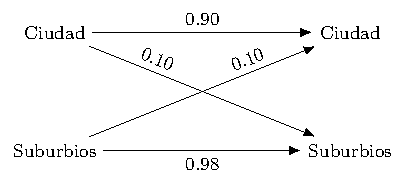
\includegraphics[width=0.55\textwidth]{figuras/cadena-ciudad-suburbios.pdf}
    \end{figure}

    La probabilidad de que un habitante de la ciudad permanezca en la ciudad durante el primer año es $0.90$, mientras que la probabilidad de que se mude a los suburbios durante el primer año es $0.10$. Por tanto, la probabilidad de que un habitante de la ciudad permanezca en la ciudad el primer año y luego se mude a los suburbios el segundo año es el producto $(0.90)(0.10)$. Análogamente, la probabilidad de que un habitante de la ciudad se mude a los suburbios el primer año y permanezca ahí el segundo año es el producto $(0.10)(0.98)$. Así, la probabilidad de que un habitante de la ciudad viva en los suburbios después de $2$ años es la suma de estos productos, $(0.90)(0.10)+(0.10)(0.98)=0.188$. Observemos que este número se obtiene mediante el mismo cálculo que produce $(A^2)_{21}$, y por tanto $(A^2)_{21}$ representa la probabilidad de que un habitante de la ciudad viva en los suburbios después de $2$ años. En general, para cualquier matriz de transición $M$, la entrada $(M^m)_{ij}$ representa la probabilidad de pasar del estado $j$ al estado $i$ en $m$ etapas.

    Supongamos además que el $70\%$ de la población de 2000 del área metropolitana vivía en la ciudad y el $30\%$ vivía en los suburbios. Registramos estos datos como un vector columna:
    \begin{equation*}
        \begin{array}{c}
            \text{Proporción de habitantes de la ciudad}\\
            \text{Proporción de residentes de los suburbios}
        \end{array}\qquad
        \begin{pmatrix}0.70\\0.30\end{pmatrix}=P.
    \end{equation*}
    Los renglones del vector $P$ corresponden a los estados de residir en la ciudad y residir en los suburbios, respectivamente, en el mismo orden que en la matriz de transición $A$. Observemos también que el vector columna $P$ tiene entradas no negativas que suman $1$.

    \begin{definicion}[Vector de probabilidad]
        Un vector columna con entradas no negativas cuya suma es $1$ se llama \textbf{vector de probabilidad}.
    \end{definicion}

    En el vector $AP$, la primera coordenada es la suma $(0.90)(0.70)+(0.02)(0.30)$. El primer término de esta suma, $(0.90)(0.70)$, representa la proporción de la población de 2000 que permaneció en la ciudad durante el año siguiente, y el segundo término, $(0.02)(0.30)$, representa la proporción que se mudó a la ciudad durante el año siguiente. Por tanto, la primera coordenada de $AP$ representa la proporción de la población metropolitana que vivía en la ciudad en 2001. Análogamente, la segunda coordenada de
    \begin{equation*}
        AP=\begin{pmatrix}0.636\\0.364\end{pmatrix}
    \end{equation*}
    representa la proporción de la población metropolitana que vivía en los suburbios en 2001. Este argumento puede extenderse fácilmente para mostrar que las coordenadas de
    \begin{equation*}
        A^2P=A(AP)=\begin{pmatrix}0.57968\\0.42032\end{pmatrix}
    \end{equation*}
    representan las proporciones de la población metropolitana que vivían en cada región en 2002. En general, las coordenadas de $A^mP$ representan la proporción de la población metropolitana que vivirá en la ciudad y en los suburbios, respectivamente, después de $m$ etapas ($m$ años después de 2000).

    ¿Se despoblará eventualmente la ciudad si esta tendencia continúa? Es natural definir la proporción eventual de habitantes de la ciudad y de los suburbios, respectivamente, como las coordenadas de $\lim_{m\to\infty}A^mP$. Calculamos ahora este límite. Es fácil ver que $A$ es diagonalizable, y que existen una matriz invertible $Q$ y una matriz diagonal $D$ tales que $Q^{-1}AQ=D$. De hecho,
    \begin{equation*}
        Q=\begin{pmatrix}\frac16&-\frac16\\\frac56&\frac16\end{pmatrix} \qquad\text{y}\qquad D=\begin{pmatrix}1&0\\0&0.88\end{pmatrix}.
    \end{equation*}
    Por tanto
    \begin{equation*}
        L=\lim_{m\to\infty}A^m=\lim_{m\to\infty}QD^mQ^{-1}=Q\begin{pmatrix}1&0\\0&0\end{pmatrix}Q^{-1}=\begin{pmatrix}\frac16&\frac16\\\frac56&\frac56\end{pmatrix}.
    \end{equation*}
    En consecuencia,
    \begin{equation*}
        \lim_{m\to\infty}A^mP=LP=\begin{pmatrix}\frac16\\\frac56\end{pmatrix}.
    \end{equation*}
    Así, eventualmente, $\frac16$ de la población vivirá en la ciudad y $\frac56$ vivirá en los suburbios cada año. Observemos que el vector $LP$ satisface $A(LP)=LP$. Por tanto, $LP$ es a la vez un vector de probabilidad y un vector propio de $A$ correspondiente al valor propio $1$. Como el subespacio propio de $A$ correspondiente al valor propio $1$ tiene dimensión uno, este es el único vector propio de esta forma, y por tanto es independiente de la elección inicial del vector de probabilidad $P$. (De hecho, si la población de 2000 del área metropolitana hubiera consistido enteramente de habitantes de la ciudad, el resultado límite habría sido el mismo.)

    En el análisis del problema ciudad-suburbios, dimos interpretaciones probabilísticas de $A^2$ y $AP$, mostrando que $A^2$ es una matriz de transición y que $AP$ es un vector de probabilidad. De hecho, el producto de dos matrices de transición cualesquiera es una matriz de transición, y el producto de cualquier matriz de transición con un vector de probabilidad es un vector de probabilidad. Estos hechos son un corolario sencillo del siguiente teorema, que caracteriza a las matrices de transición y a los vectores de probabilidad.

    \begin{teorema}
        Sea $M$ una matriz $n\times n$ con entradas reales no negativas, sea $v$ un vector columna en $\R^n$ con coordenadas no negativas, y sea $u\in\R^n$ el vector columna cuya coordenada es $1$ en cada entrada. Entonces:
        \begin{enumerate}[label=(\alph*)]
            \item $M$ es una matriz de transición si y solo si $M^tu=u$.
            \item $v$ es un vector de probabilidad si y solo si $u^tv=(1)$.
        \end{enumerate}
    \end{teorema}

    \begin{proof}
        (a) Para cada $j$ ($1\leq j\leq n$),
        \begin{equation*}
            (M^tu)_j=\sum_{i=1}^{n}(M^t)_{ji}u_i=\sum_{i=1}^{n}M_{ij}\cdot 1=\sum_{i=1}^{n}M_{ij},
        \end{equation*}
        que es precisamente la suma de la columna $j$ de $M$. Como las entradas de $M$ son no negativas por hipótesis, $M$ es una matriz de transición (es decir, la suma de cada columna es $1$) si y solo si $(M^tu)_j=u_j=1$ para todo $j$, es decir, si y solo si $M^tu=u$.

        (b) $u^tv=\sum_{i=1}^{n}v_i$, la suma de las entradas de $v$. Como $v$ tiene coordenadas no negativas por hipótesis, $v$ es un vector de probabilidad (es decir, la suma de sus entradas es $1$) si y solo si $u^tv=(1)$.
    \end{proof}

    \begin{corolario}\leavevmode
        \begin{enumerate}[label=(\alph*)]
            \item El producto de dos matrices de transición $n\times n$ es una matriz de transición $n\times n$. En particular, cualquier potencia de una matriz de transición es una matriz de transición.
            \item El producto de una matriz de transición y un vector de probabilidad es un vector de probabilidad.
        \end{enumerate}
    \end{corolario}

    \begin{proof}
        (a) Sean $M,N$ matrices de transición $n\times n$. Como $M$ y $N$ tienen entradas no negativas, también las tiene $MN$. Además, usando el teorema anterior,
        \begin{equation*}
            (MN)^tu=N^tM^tu=N^tu=u,
        \end{equation*}
        así que $MN$ es una matriz de transición por el teorema anterior. Para las potencias, basta aplicar este resultado repetidamente: $M^2=MM$ es una matriz de transición, y por inducción, $M^{k}=M^{k-1}M$ es una matriz de transición para todo $k\geq 1$.

        (b) Sea $M$ una matriz de transición $n\times n$ y $v$ un vector de probabilidad en $\R^n$. Como $M$ y $v$ tienen entradas no negativas, también las tiene $Mv$. Además, usando que $u^tM=(M^tu)^t=u^t$ por el teorema anterior, y que $u^tv=(1)$,
        \begin{equation*}
            u^t(Mv)=(u^tM)v=u^tv=(1),
        \end{equation*}
        así que $Mv$ es un vector de probabilidad por el teorema anterior.
    \end{proof}

    El problema ciudad-suburbios es un ejemplo de un proceso en el cual los elementos de un conjunto se clasifican en uno de varios estados fijos, y cambian de estado con el tiempo. En general, un proceso de este tipo se llama \textbf{proceso estocástico}. El cambio a un estado particular se describe mediante una probabilidad, y en general esta probabilidad depende de factores como el estado en cuestión, el tiempo en cuestión, algunos o todos los estados previos en los que ha estado el objeto (incluyendo el estado actual), y los estados en los que se encuentran o han estado otros objetos.

    Si, sin embargo, la probabilidad de que un objeto en un estado cambie a un estado diferente en un intervalo fijo de tiempo depende únicamente de los dos estados (y no del tiempo, de estados anteriores, ni de otros factores), entonces el proceso estocástico se llama \textbf{proceso de Markov}. Si, además, el número de estados posibles es finito, entonces el proceso de Markov se llama \textbf{cadena de Markov}. El problema ciudad-suburbios es una cadena de Markov de dos estados. Por supuesto, un proceso de Markov suele ser solo una idealización de la realidad, pues las probabilidades involucradas casi nunca son constantes.

    Con esto en mente, consideramos otra cadena de Markov. Cierta universidad comunitaria desearía obtener información sobre la probabilidad de que los estudiantes en distintas categorías se gradúen. La escuela clasifica a un estudiante como de segundo año o de primer año dependiendo del número de créditos que ha obtenido. Los datos de la escuela indican que, de un semestre de otoño al siguiente, el $40\%$ de los estudiantes de segundo año se graduará, el $30\%$ permanecerá como estudiante de segundo año, y el $30\%$ abandonará permanentemente. Para los estudiantes de primer año, los datos muestran que el $10\%$ se graduará al siguiente otoño, el $50\%$ pasará a segundo año, el $20\%$ permanecerá como estudiante de primer año, y el $20\%$ abandonará permanentemente. Durante el año en curso, el $50\%$ de los estudiantes de la escuela son de segundo año y el $50\%$ son de primer año. Suponiendo que la tendencia indicada por los datos continúa indefinidamente, la escuela desearía saber:
    \begin{enumerate}
        \item el porcentaje de los estudiantes actuales que se graduará, el porcentaje que será de segundo año, el porcentaje que será de primer año, y el porcentaje que abandonará permanentemente para el próximo otoño;
        \item los mismos porcentajes del inciso~1 para el semestre de otoño dos años después; y
        \item la probabilidad de que uno de los estudiantes actuales eventualmente se gradúe.
    \end{enumerate}

    El párrafo anterior describe una cadena de Markov de cuatro estados con los siguientes estados: 1. haberse graduado; 2. ser estudiante de segundo año; 3. ser estudiante de primer año; 4. haber abandonado permanentemente. Los datos dados nos proporcionan la matriz de transición
    \begin{equation*}
        A=\begin{pmatrix}1&0.4&0.1&0\\0&0.3&0.5&0\\0&0&0.2&0\\0&0.3&0.2&1\end{pmatrix}
    \end{equation*}
    de la cadena de Markov. (Nótese que se supone que los estudiantes que se han graduado o han abandonado permanecen indefinidamente en esos respectivos estados.) Además, se nos dice que la distribución actual de estudiantes es la mitad en cada uno de los estados 2 y 3, y ninguno en los estados 1 y 4. El vector
    \begin{equation*}
        P=\begin{pmatrix}0\\0.5\\0.5\\0\end{pmatrix}
    \end{equation*}
    que describe la probabilidad inicial de estar en cada estado se llama el \textbf{vector de probabilidad inicial} de la cadena de Markov.

    Para responder la pregunta 1, debemos determinar las probabilidades de que un estudiante actual esté en cada estado para el próximo otoño. Como hemos visto, estas probabilidades son las coordenadas del vector
    \begin{equation*}
        AP=\begin{pmatrix}1&0.4&0.1&0\\0&0.3&0.5&0\\0&0&0.2&0\\0&0.3&0.2&1\end{pmatrix}\begin{pmatrix}0\\0.5\\0.5\\0\end{pmatrix}=\begin{pmatrix}0.25\\0.40\\0.10\\0.25\end{pmatrix}.
    \end{equation*}
    Así, para el próximo otoño, el $25\%$ de los estudiantes actuales se graduará, el $40\%$ será de segundo año, el $10\%$ será de primer año, y el $25\%$ abandonará la escuela permanentemente. Análogamente,
    \begin{equation*}
        A^2P=A(AP)=\begin{pmatrix}1&0.4&0.1&0\\0&0.3&0.5&0\\0&0&0.2&0\\0&0.3&0.2&1\end{pmatrix}\begin{pmatrix}0.25\\0.40\\0.10\\0.25\end{pmatrix}=\begin{pmatrix}0.42\\0.17\\0.02\\0.39\end{pmatrix}
    \end{equation*}
    proporciona la información necesaria para responder la pregunta 2: dentro de dos años, el $42\%$ de los estudiantes actuales se graduará, el $17\%$ será de segundo año, el $2\%$ será de primer año, y el $39\%$ abandonará la escuela.

    Finalmente, la respuesta a la pregunta 3 la proporciona el vector $LP$, donde $L=\lim_{m\to\infty}A^m$. Para las matrices
    \begin{equation*}
        Q=\begin{pmatrix}1&4&19&0\\0&-7&-40&0\\0&0&8&0\\0&3&13&1\end{pmatrix} \qquad\text{y}\qquad D=\begin{pmatrix}1&0&0&0\\0&0.3&0&0\\0&0&0.2&0\\0&0&0&1\end{pmatrix},
    \end{equation*}
    tenemos $Q^{-1}AQ=D$. Así,
    \begin{equation*}
        L=\lim_{m\to\infty}A^m=Q\left(\lim_{m\to\infty}D^m\right)Q^{-1}=\begin{pmatrix}1&\frac47&\frac{27}{56}&0\\0&0&0&0\\0&0&0&0\\0&\frac37&\frac{29}{56}&1\end{pmatrix}.
    \end{equation*}
    Así,
    \begin{equation*}
        LP=\begin{pmatrix}1&\frac47&\frac{27}{56}&0\\0&0&0&0\\0&0&0&0\\0&\frac37&\frac{29}{56}&1\end{pmatrix}\begin{pmatrix}0\\0.5\\0.5\\0\end{pmatrix}=\begin{pmatrix}\frac{59}{112}\\0\\0\\\frac{53}{112}\end{pmatrix},
    \end{equation*}
    de donde la probabilidad de que uno de los estudiantes actuales se gradúe es $\frac{59}{112}$.

    En los dos ejemplos anteriores, vimos que $\lim_{m\to\infty}A^mP$, donde $A$ es la matriz de transición y $P$ es el vector de probabilidad inicial de la cadena de Markov, da las proporciones eventuales en cada estado. En general, sin embargo, el límite de las potencias de una matriz de transición no necesita existir. Por ejemplo, si
    \begin{equation*}
        M=\begin{pmatrix}0&1\\1&0\end{pmatrix},
    \end{equation*}
    entonces $\lim_{m\to\infty}M^m$ no existe, porque las potencias impares de $M$ son iguales a $M$ y las potencias pares son iguales a $I$. La razón por la que el límite no existe es que la condición (a) del Teorema~5.13 no se cumple para $M$ ($-1$ es valor propio). De hecho, se puede mostrar (aunque no lo hacemos aquí, pues su demostración requiere de nuevo la teoría de la forma canónica de Jordan) que las únicas matrices de transición $A$ tales que $\lim_{m\to\infty}A^m$ no existe son precisamente aquellas para las cuales falla la condición (a) del Teorema~5.13.

    Pero incluso si el límite de las potencias de la matriz de transición existe, el cálculo del límite puede ser bastante difícil. Afortunadamente, existe una clase amplia e importante de matrices de transición para las cuales este límite existe y es fácil de calcular: la clase de las matrices de transición \textit{regulares}.

    \begin{definicion}[Matriz de transición regular]
        Una matriz de transición se llama \textbf{regular} si alguna potencia de ella contiene únicamente entradas positivas.
    \end{definicion}

    \begin{ejemplo}
        La matriz de transición
        \begin{equation*}
            \begin{pmatrix}0.90&0.02\\0.10&0.98\end{pmatrix}
        \end{equation*}
        de la cadena de Markov usada en el problema ciudad-suburbios es claramente regular porque cada entrada es positiva. Por otro lado, la matriz de transición
        \begin{equation*}
            A=\begin{pmatrix}1&0.4&0.1&0\\0&0.3&0.5&0\\0&0&0.2&0\\0&0.3&0.2&1\end{pmatrix}
        \end{equation*}
        de la cadena de Markov que describe las matrículas de la universidad comunitaria no es regular, pues la primera columna de $A^m$ es
        \begin{equation*}
            \begin{pmatrix}1\\0\\0\\0\end{pmatrix}
        \end{equation*}
        para cualquier potencia $m$. Observemos que una matriz de transición regular puede contener entradas nulas. Por ejemplo,
        \begin{equation*}
            M=\begin{pmatrix}0.9&0.5&0\\0&0.5&0.4\\0.1&0&0.6\end{pmatrix}
        \end{equation*}
        es regular porque cada entrada de $M^2$ es positiva.
    \end{ejemplo}

    El resto de esta sección se dedica a probar que, para una matriz de transición regular $A$, el límite de la sucesión de potencias de $A$ existe y tiene columnas idénticas. A partir de este hecho, es fácil calcular dicho límite. En el curso de la demostración de este resultado, obtenemos algunas cotas interesantes para las magnitudes de los valores propios de cualquier matriz cuadrada. Estas cotas se expresan en términos de la suma de los valores absolutos de los renglones y columnas de la matriz. La terminología necesaria se introduce en las siguientes definiciones.

    \begin{definicion}[Suma de renglón y suma de columna]
        Sea $A\in M_{n\times n}(\C)$. Para $1\leq i,j\leq n$, se define $\rho_i(A)$ como la suma de los valores absolutos de las entradas del renglón $i$ de $A$, y se define $\nu_j(A)$ como la suma de los valores absolutos de las entradas de la columna $j$ de $A$. Así,
        \begin{equation*}
            \rho_i(A)=\sum_{j=1}^{n}|A_{ij}| \quad\text{para } i=1,2,\dots,n
        \end{equation*}
        y
        \begin{equation*}
            \nu_j(A)=\sum_{i=1}^{n}|A_{ij}| \quad\text{para } j=1,2,\dots,n.
        \end{equation*}
        La \textbf{suma de renglón} de $A$, denotada $\rho(A)$, y la \textbf{suma de columna} de $A$, denotada $\nu(A)$, se definen como
        \begin{equation*}
            \rho(A)=\max\{\rho_i(A):1\leq i\leq n\} \qquad\text{y}\qquad \nu(A)=\max\{\nu_j(A):1\leq j\leq n\}.
        \end{equation*}
    \end{definicion}

    \begin{ejemplo}
        Para la matriz
        \begin{equation*}
            A=\begin{pmatrix}1&-i&3-4i\\-2+i&0&6\\3&2&i\end{pmatrix},
        \end{equation*}
        tenemos $\rho_1(A)=7$, $\rho_2(A)=6+\sqrt5$, $\rho_3(A)=6$, $\nu_1(A)=4+\sqrt5$, $\nu_2(A)=3$, y $\nu_3(A)=12$. Por tanto $\rho(A)=6+\sqrt5$ y $\nu(A)=12$.
    \end{ejemplo}

    Nuestros próximos resultados muestran que la menor de $\rho(A)$ y $\nu(A)$ es una cota para los valores absolutos de los valores propios de $A$. En el ejemplo anterior, por ejemplo, $A$ no tiene ningún valor propio con valor absoluto mayor que $6+\sqrt5$. Para obtener una visión geométrica del siguiente teorema, introducimos algo de terminología: para una matriz $A\in M_{n\times n}(\C)$, se define el $i$-ésimo \textbf{disco de Gerschgorin} $C_i$ como el disco en el plano complejo con centro $A_{ii}$ y radio $r_i=\rho_i(A)-|A_{ii}|$; es decir,
    \begin{equation*}
        C_i=\{z\in\C:|z-A_{ii}|<r_i\}.
    \end{equation*}

    \begin{definicion}[Disco de Gerschgorin]
        Sea $A\in M_{n\times n}(\C)$. Para cada $i$ ($1\leq i\leq n$), el \textbf{$i$-ésimo disco de Gerschgorin} $C_i$ de $A$ es el disco en el plano complejo con centro $A_{ii}$ y radio $r_i=\rho_i(A)-|A_{ii}|$, es decir,
        \begin{equation*}
            C_i=\{z\in\C:|z-A_{ii}|<r_i\}.
        \end{equation*}
    \end{definicion}

    Por ejemplo, consideremos la matriz
    \begin{equation*}
        A=\begin{pmatrix}1+2i&1\\2i&-3\end{pmatrix}.
    \end{equation*}
    Para esta matriz, $C_1$ es el disco con centro $1+2i$ y radio $1$, y $C_2$ es el disco con centro $-3$ y radio $2$. (Véase la siguiente figura.)

    \begin{figure}[H]
        \centering
        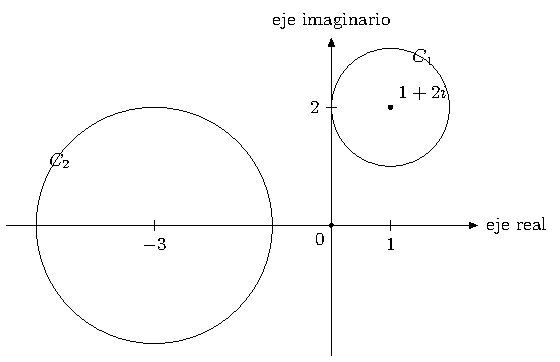
\includegraphics[width=0.6\textwidth]{figuras/discos-gerschgorin.pdf}
    \end{figure}

    El teorema del disco de Gerschgorin, enunciado a continuación, nos dice que todos los valores propios de $A$ están ubicados dentro de estos dos discos.

    \begin{teorema}[Disco de Gerschgorin]
        Sea $A\in M_{n\times n}(\C)$. Entonces todo valor propio de $A$ está contenido en algún disco de Gerschgorin de $A$.
    \end{teorema}

    \begin{proof}
        Sea $\lambda$ un valor propio de $A$ con vector propio correspondiente
        \begin{equation*}
            v=\begin{pmatrix}v_1\\v_2\\\vdots\\v_n\end{pmatrix}.
        \end{equation*}
        Entonces $v$ satisface la ecuación matricial $Av=\lambda v$, que puede escribirse
        \begin{equation*}
            \sum_{j=1}^{n}A_{ij}v_j=\lambda v_i \qquad (i=1,2,\dots,n). \tag{$*$}
        \end{equation*}
        Supongamos que $v_k$ es la coordenada de $v$ que tiene el mayor valor absoluto; notemos que $v_k\neq 0$ porque $v$ es un vector propio. Mostramos que $\lambda$ está en $C_k$, es decir, que $|\lambda-A_{kk}|\leq r_k$. Para $i=k$, se sigue de ($*$) que
        \begin{align*}
            |\lambda v_k-A_{kk}v_k|=\left|\sum_{j=1}^{n}A_{kj}v_j-A_{kk}v_k\right|=\left|\sum_{j\neq k}A_{kj}v_j\right|
            &\leq\sum_{j\neq k}|A_{kj}||v_j|\leq\sum_{j\neq k}|A_{kj}||v_k|\\
            &=|v_k|\sum_{j\neq k}|A_{kj}|=|v_k|r_k.
        \end{align*}
        Así,
        \begin{equation*}
            |v_k||\lambda-A_{kk}|\leq|v_k|r_k;
        \end{equation*}
        por lo cual $|\lambda-A_{kk}|\leq r_k$, ya que $|v_k|>0$.
    \end{proof}

    \begin{corolario}
        Sea $\lambda$ cualquier valor propio de $A\in M_{n\times n}(\C)$. Entonces $|\lambda|\leq\rho(A)$.
    \end{corolario}

    \begin{proof}
        Por el teorema del disco de Gerschgorin, $|\lambda-A_{kk}|\leq r_k$ para algún $k$. Por tanto
        \begin{equation*}
            |\lambda|=|(\lambda-A_{kk})+A_{kk}|\leq|\lambda-A_{kk}|+|A_{kk}|\leq r_k+|A_{kk}|=\rho_k(A)\leq\rho(A).
        \end{equation*}
    \end{proof}

    \begin{corolario}
        Sea $\lambda$ cualquier valor propio de $A\in M_{n\times n}(\C)$. Entonces
        \begin{equation*}
            |\lambda|\leq\min\{\rho(A),\nu(A)\}.
        \end{equation*}
    \end{corolario}

    \begin{proof}
        Por el corolario anterior, $|\lambda|\leq\rho(A)$; basta entonces mostrar que $|\lambda|\leq\nu(A)$. Como $\lambda$ es también valor propio de $A^t$ (pues $A$ y $A^t$ tienen el mismo polinomio característico), el corolario anterior aplicado a $A^t$ da $|\lambda|\leq\rho(A^t)$. Pero los renglones de $A^t$ son las columnas de $A$; en consecuencia $\rho(A^t)=\nu(A)$. Por tanto $|\lambda|\leq\nu(A)$.
    \end{proof}

    \begin{corolario}
        Si $\lambda$ es un valor propio de una matriz de transición, entonces $|\lambda|\leq 1$.
    \end{corolario}

    \begin{proof}
        Si $A$ es una matriz de transición, entonces cada columna de $A$ suma exactamente $1$, así que $\nu(A)=1$. Por el corolario anterior, $|\lambda|\leq\nu(A)=1$.
    \end{proof}

    Supongamos que $A$ es una matriz de transición para la cual algún vector propio correspondiente al valor propio $1$ tiene solo coordenadas no negativas. Entonces algún múltiplo de este vector es un vector de probabilidad $P$ y, a la vez, un vector propio de $A$ correspondiente al valor propio $1$. Es interesante observar que, si $P$ es el vector de probabilidad inicial de una cadena de Markov cuya matriz de transición es $A$, entonces $A^mP=P$ para todo entero positivo $m$; de aquí que la probabilidad de estar en cada estado nunca cambia. (Recordemos el problema ciudad-suburbios con $P=\left(\begin{smallmatrix}\frac16\\\frac56\end{smallmatrix}\right)$.)

    \begin{teorema}
        Sea $A\in M_{n\times n}(\C)$ una matriz en la que cada entrada es positiva, y sea $\lambda$ un valor propio de $A$ tal que $|\lambda|=\rho(A)$. Entonces $\lambda=\rho(A)$, y $\{u\}$ es una base de $E_\lambda$, donde $u\in\C^n$ es el vector columna en el que cada coordenada es igual a $1$.
    \end{teorema}

    \begin{proof}
        Sea $v$ un vector propio de $A$ correspondiente a $\lambda$, con coordenadas $v_1,v_2,\dots,v_n$. Supongamos que $v_k$ es la coordenada de $v$ con mayor valor absoluto, y sea $b=|v_k|$. Entonces
        \begin{align*}
            |\lambda|b=|\lambda||v_k|=|\lambda v_k|=\left|\sum_{j=1}^{n}A_{kj}v_j\right|
            &\leq\sum_{j=1}^{n}|A_{kj}v_j|\\
            &=\sum_{j=1}^{n}|A_{kj}||v_j|\leq\sum_{j=1}^{n}|A_{kj}|b=\rho_k(A)b\leq\rho(A)b. \tag{3}
        \end{align*}
        Como $|\lambda|=\rho(A)$, las tres desigualdades en (3) son en realidad igualdades; es decir,
        \begin{enumerate}
            \item[(a)] $\left|\sum_{j=1}^{n}A_{kj}v_j\right|=\sum_{j=1}^{n}|A_{kj}v_j|$,
            \item[(b)] $\sum_{j=1}^{n}|A_{kj}||v_j|=\sum_{j=1}^{n}|A_{kj}|b$, y
            \item[(c)] $\rho_k(A)=\rho(A)$.
        \end{enumerate}
        La igualdad (a) obliga a que todos los términos $A_{kj}v_j$ ($j=1,2,\dots,n$) sean múltiplos no negativos de algún número complejo no nulo $z$ (pues, en general, la igualdad $|\sum_j w_j|=\sum_j|w_j|$ para números complejos $w_j$ se da si y solo si todos los $w_j$ apuntan en la misma dirección, es decir, son múltiplos no negativos de un mismo $z$ con $|z|=1$, que podemos suponer sin pérdida de generalidad). Así, existen números reales no negativos $c_1,c_2,\dots,c_n$ tales que
        \begin{equation*}
            A_{kj}v_j=c_jz \qquad\text{para } j=1,2,\dots,n. \tag{4}
        \end{equation*}
        Por (b), y como $A_{kj}\neq 0$ para todo $k$ y $j$ (pues $A$ tiene entradas positivas),
        \begin{equation*}
            |v_j|=b \qquad\text{para } j=1,2,\dots,n. \tag{5}
        \end{equation*}
        Combinando (4) y (5), obtenemos
        \begin{equation*}
            b=|v_j|=\left|\frac{c_j}{A_{kj}}z\right|=\frac{c_j}{A_{kj}} \qquad\text{para } j=1,2,\dots,n,
        \end{equation*}
        y por tanto, por (4), $v_j=bz$ para todo $j$. Así,
        \begin{equation*}
            v=\begin{pmatrix}v_1\\v_2\\\vdots\\v_n\end{pmatrix}=\begin{pmatrix}bz\\bz\\\vdots\\bz\end{pmatrix}=bzu,
        \end{equation*}
        y por tanto $\{u\}$ es una base de $E_\lambda$.

        Finalmente, observemos que todas las entradas de $Au$ son positivas, pues lo son las de $A$ y las de $u$. Pero $Au=\lambda u$, y por tanto $\lambda>0$. En consecuencia, $\lambda=|\lambda|=\rho(A)$.
    \end{proof}

    \begin{corolario}
        Sea $A\in M_{n\times n}(\C)$ una matriz en la que cada entrada es positiva, y sea $\lambda$ un valor propio de $A$ tal que $|\lambda|=\nu(A)$. Entonces $\lambda=\nu(A)$, y $\dim(E_\lambda)=1$.
    \end{corolario}

    \begin{proof}
        Como $A$ tiene entradas positivas, también las tiene $A^t$. Además, $\lambda$ es también un valor propio de $A^t$ (pues $A$ y $A^t$ tienen el mismo polinomio característico), y $|\lambda|=\nu(A)=\rho(A^t)$ (ya que los renglones de $A^t$ son las columnas de $A$). Aplicando el teorema anterior a $A^t$, obtenemos $\lambda=\rho(A^t)=\nu(A)$, y que $\{u\}$ es una base del subespacio propio $\ker(A^t-\lambda I)$; en particular, $\dim\ker(A^t-\lambda I)=1$.

        Finalmente, para cualquier matriz cuadrada $B$, se tiene $\dim\ker(B)=\dim\ker(B^t)$, pues $\rg(B)=\rg(B^t)$ y, por el teorema de la dimensión, $\dim\ker(B)=n-\rg(B)=n-\rg(B^t)=\dim\ker(B^t)$. Aplicando esto a $B=A-\lambda I$ (de modo que $B^t=A^t-\lambda I$),
        \begin{equation*}
            \dim(E_\lambda)=\dim\ker(A-\lambda I)=\dim\ker(A^t-\lambda I)=1.
        \end{equation*}
    \end{proof}

    \begin{corolario}
        Sea $A\in M_{n\times n}(\C)$ una matriz de transición en la que cada entrada es positiva, y sea $\lambda$ cualquier valor propio de $A$ distinto de $1$. Entonces $|\lambda|<1$. Más aún, el subespacio propio correspondiente al valor propio $1$ tiene dimensión $1$.
    \end{corolario}

    \begin{proof}
        Como $A$ es una matriz de transición, $\nu(A)=1$. Supongamos que $\lambda$ es un valor propio de $A$ con $|\lambda|=\nu(A)=1$. Por el corolario anterior, $\lambda=\nu(A)=1$. Así, ningún valor propio distinto de $1$ puede tener $|\lambda|=1$; combinando esto con el Corolario anterior a este (el que afirma $|\lambda|\leq 1$ para toda matriz de transición), concluimos que todo valor propio $\lambda\neq 1$ satisface $|\lambda|<1$.

        Finalmente, como $\lambda=1$ sí satisface $|\lambda|=\nu(A)=1$, el corolario anterior (aplicado con $\lambda=1$) da $\dim(E_1)=1$.
    \end{proof}

    El siguiente resultado extiende el corolario anterior a las matrices de transición regulares, y así muestra que las matrices de transición regulares satisfacen la condición (a) de los Teoremas~5.13 y 1.14.

    \begin{teorema}
        Sea $A$ una matriz de transición regular, y sea $\lambda$ un valor propio de $A$. Entonces:
        \begin{enumerate}[label=(\alph*)]
            \item $|\lambda|\leq 1$.
            \item Si $|\lambda|=1$, entonces $\lambda=1$, y $\dim(E_\lambda)=1$.
        \end{enumerate}
    \end{teorema}

    \begin{proof}
        El inciso (a) ya fue probado (es el corolario al teorema del disco de Gerschgorin sobre matrices de transición).

        (b) Como $A$ es regular, existe un entero positivo $s$ tal que $A^s$ tiene solo entradas positivas. Como $A$ es una matriz de transición, las entradas de $A^{s+1}=A^s(A)$ también son positivas (por el corolario al Teorema~5.15, $A^{s+1}$ es una matriz de transición cuyas entradas, al ser producto de entradas no negativas de matrices con la estructura adecuada, resultan positivas al serlo las de $A^s$ y ser $A$ de transición con al menos una entrada positiva por columna). Supongamos que $|\lambda|=1$. Entonces $\lambda^s$ y $\lambda^{s+1}$ son valores propios de $A^s$ y $A^{s+1}$, respectivamente, ambos con valor absoluto $1$. Así, por el corolario anterior aplicado a $A^s$ y a $A^{s+1}$ (ambas con entradas positivas), $\lambda^s=1=\lambda^{s+1}$. Por tanto $\lambda=1$.

        Sean $E_\lambda$ y $E_\lambda'$ los subespacios propios de $A$ y de $A^s$, respectivamente, correspondientes a $\lambda=1$. Entonces $E_\lambda\subseteq E_\lambda'$ (pues si $Av=v$ entonces $A^sv=v$), y, por el corolario anterior aplicado a $A^s$, $\dim(E_\lambda')=1$. Como $\dim(E_\lambda)\geq 1$ (pues $1$ es valor propio de $A$, por lo probado anteriormente para matrices de transición con entradas positivas aplicado a $A^s$, y por la inclusión $E_\lambda \subseteq E_\lambda'$), concluimos $\dim(E_\lambda)=1$.
    \end{proof}

    \begin{corolario}
        Sea $A$ una matriz de transición regular que además es diagonalizable. Entonces $\lim_{m\to\infty}A^m$ existe.
    \end{corolario}

    \begin{proof}
        Por el teorema anterior, todo valor propio $\lambda$ de $A$ satisface $|\lambda|\leq 1$, con $\lambda=1$ siempre que $|\lambda|=1$; es decir, todo valor propio de $A$ está en $S$. Como además $A$ es diagonalizable por hipótesis, se cumplen las dos condiciones del Teorema~5.14, y por tanto $\lim_{m\to\infty}A^m$ existe.
    \end{proof}

    El corolario anterior, que se sigue inmediatamente del teorema anterior y del Teorema~5.14, no es el mejor resultado posible. De hecho, puede mostrarse (aunque, de nuevo, ello requiere la teoría de la forma canónica de Jordan) que si $A$ es una matriz de transición regular, entonces la multiplicidad de $1$ como valor propio de $A$ es $1$; así, por el Teorema~5.13, $\lim_{m\to\infty}A^m$ existe sin importar si $A$ es o no diagonalizable. Sin importar la diagonalizabilidad de $A$, deducimos aquí más hechos sobre $\lim_{m\to\infty}A^m$ cuando $A$ es una matriz de transición regular, dando por cierto (sin demostrarlo, pues su prueba pertenece a un curso posterior) el hecho de que la multiplicidad de $1$ es siempre $1$ para una matriz de transición regular.

    \begin{teorema}
        Sea $A$ una matriz de transición regular de tamaño $n\times n$. Entonces:
        \begin{enumerate}[label=(\alph*)]
            \item La multiplicidad de $1$ como valor propio de $A$ es $1$.
            \item $\lim_{m\to\infty}A^m$ existe.
            \item $L=\lim_{m\to\infty}A^m$ es una matriz de transición.
            \item $AL=LA=L$.
            \item Las columnas de $L$ son idénticas. De hecho, cada columna de $L$ es igual al único vector de probabilidad $v$ que es también un vector propio de $A$ correspondiente al valor propio $1$.
            \item Para cualquier vector de probabilidad $w$, $\lim_{m\to\infty}(A^mw)=v$.
        \end{enumerate}
    \end{teorema}

    \begin{proof}
        El inciso (a) requiere la teoría de la forma canónica de Jordan y no se demuestra en este curso.

        (b) Por (a) y los Teoremas~5.18 y 1.13, todo valor propio de $A$ está en $S$ (por el teorema anterior a este) y la multiplicidad de $1$ coincide con $\dim(E_1)$ (por (a), ambas son $1$). Así, se cumplen las condiciones (a) y (b) del Teorema~5.13, y por tanto $\lim_{m\to\infty}A^m$ existe.

        (c) Por el Teorema~5.15, basta mostrar que $u^tL=u^t$. Como $A^m$ es una matriz de transición por el corolario al Teorema~5.15,
        \begin{equation*}
            u^tL=u^t\lim_{m\to\infty}A^m=\lim_{m\to\infty}u^tA^m=\lim_{m\to\infty}u^t=u^t,
        \end{equation*}
        de donde se sigue que $L$ es una matriz de transición.

        (d) Por el Teorema~5.12,
        \begin{equation*}
            AL=A\lim_{m\to\infty}A^m=\lim_{m\to\infty}AA^m=\lim_{m\to\infty}A^{m+1}=L.
        \end{equation*}
        Análogamente, $LA=L$.

        (e) Como $AL=L$ por (d), cada columna de $L$ es un vector propio de $A$ correspondiente al valor propio $1$. Más aún, por (c), cada columna de $L$ es un vector de probabilidad. Así, por (a), cada columna de $L$ es igual al único vector de probabilidad $v$ correspondiente al valor propio $1$ de $A$.

        (f) Sea $w$ cualquier vector de probabilidad, y sea $y=\lim_{m\to\infty}A^mw=Lw$. Entonces $y$ es un vector de probabilidad por el corolario al Teorema~5.15, y también es un vector propio correspondiente al valor propio $1$ de $A$, pues $Ay=ALw=Lw=y$ por (d). Así $y=v$ por (e).
    \end{proof}

    \begin{definicion}[Vector de probabilidad fijo]
        Al vector $v$ del inciso (e) del teorema anterior se le llama \textbf{vector de probabilidad fijo} o \textbf{vector estacionario} de la matriz de transición regular $A$.
    \end{definicion}

    El teorema anterior puede usarse para deducir información sobre la distribución eventual en cada estado de una cadena de Markov cuya matriz de transición es regular.

    \begin{ejemplo}
        Una encuesta en Persia mostró que, en cierto día, el $50\%$ de los persas prefería una hogaza de pan, el $30\%$ prefería una jarra de vino, y el $20\%$ prefería \textquotedblleft aquello a mi lado en el desierto\textquotedblright. Una encuesta subsecuente, un mes después, arrojó los siguientes datos: de quienes preferían una hogaza de pan en la primera encuesta, el $40\%$ siguió prefiriendo una hogaza de pan, el $10\%$ ahora prefería una jarra de vino, y el $50\%$ prefería \textquotedblleft aquello\textquotedblright; de quienes preferían una jarra de vino en la primera encuesta, el $20\%$ ahora prefería una hogaza de pan, el $70\%$ seguía prefiriendo la jarra de vino, y el $10\%$ ahora prefería \textquotedblleft aquello\textquotedblright; de quienes preferían \textquotedblleft aquello\textquotedblright\ en la primera encuesta, el $20\%$ prefería ahora una hogaza de pan, el $20\%$ prefería una jarra de vino, y el $60\%$ seguía prefiriendo \textquotedblleft aquello\textquotedblright.

        Suponiendo que esta tendencia continúa, la situación descrita en el párrafo anterior es una cadena de Markov de tres estados en la cual los estados son las tres preferencias posibles. Podemos predecir el porcentaje de persas en cada estado para cada mes siguiente a la encuesta original. Denotando el primer, segundo y tercer estado como las preferencias por pan, vino y \textquotedblleft aquello\textquotedblright, respectivamente, vemos que el vector de probabilidad que da la probabilidad inicial de estar en cada estado es
        \begin{equation*}
            P=\begin{pmatrix}0.50\\0.30\\0.20\end{pmatrix},
        \end{equation*}
        y que la matriz de transición es
        \begin{equation*}
            A=\begin{pmatrix}0.40&0.20&0.20\\0.10&0.70&0.20\\0.50&0.10&0.60\end{pmatrix}.
        \end{equation*}
        Las probabilidades de estar en cada estado $m$ meses después de la encuesta original son las coordenadas del vector $A^mP$. Se puede verificar que
        \begin{equation*}
            AP=\begin{pmatrix}0.30\\0.30\\0.40\end{pmatrix}, \quad A^2P=\begin{pmatrix}0.26\\0.32\\0.42\end{pmatrix}, \quad A^3P=\begin{pmatrix}0.252\\0.334\\0.414\end{pmatrix}, \quad\text{y}\quad A^4P=\begin{pmatrix}0.2504\\0.3418\\0.4078\end{pmatrix}.
        \end{equation*}
        Observemos la aparente convergencia de $A^mP$.

        Como $A$ es regular, la predicción a largo plazo sobre las preferencias de los persas puede encontrarse calculando el vector de probabilidad fijo para $A$. Este vector es el único vector de probabilidad $v$ tal que $(A-I)v=0$. Escribiendo
        \begin{equation*}
            v=\begin{pmatrix}v_1\\v_2\\v_3\end{pmatrix},
        \end{equation*}
        vemos que la ecuación matricial $(A-I)v=0$ produce el siguiente sistema de ecuaciones lineales:
        \begin{align*}
            -0.60v_1+0.20v_2+0.20v_3&=0\\
            0.10v_1-0.30v_2+0.20v_3&=0\\
            0.50v_1+0.10v_2-0.40v_3&=0.
        \end{align*}
        Se muestra fácilmente que
        \begin{equation*}
            \begin{pmatrix}5\\7\\8\end{pmatrix}
        \end{equation*}
        es una base del espacio solución de este sistema. Por tanto, el único vector de probabilidad fijo de $A$ es
        \begin{equation*}
            \begin{pmatrix}\frac{5}{5+7+8}\\[0.5ex]\frac{7}{5+7+8}\\[0.5ex]\frac{8}{5+7+8}\end{pmatrix}=\begin{pmatrix}0.25\\0.35\\0.40\end{pmatrix}.
        \end{equation*}
        Así, a largo plazo, el $25\%$ de los persas preferirá una hogaza de pan, el $35\%$ preferirá una jarra de vino, y el $40\%$ preferirá \textquotedblleft aquello a mi lado en el desierto\textquotedblright.
    \end{ejemplo}

    En esta sección nos hemos concentrado principalmente en la teoría de las matrices de transición regulares. Existe otra clase interesante de matrices de transición que puede representarse en la forma
    \begin{equation*}
        \begin{pmatrix}I&B\\O&C\end{pmatrix},
    \end{equation*}
    donde $I$ es una matriz identidad y $O$ es una matriz cero. (Tales matrices de transición no son regulares, pues el bloque inferior izquierdo permanece igual a $O$ en cualquier potencia de la matriz.)

    \begin{definicion}[Estados absorbentes]
        Los estados correspondientes a la submatriz identidad de una matriz de transición de la forma anterior se llaman \textbf{estados absorbentes}, pues tal estado nunca se abandona una vez que se entra en él. Una cadena de Markov se llama \textbf{cadena de Markov absorbente} si es posible pasar de cualquier estado a algún estado absorbente en un número finito de etapas.
    \end{definicion}

    Observemos que la cadena de Markov que describe el patrón de matrícula de la universidad comunitaria es una cadena de Markov absorbente, con los estados 1 y 4 como sus estados absorbentes.

    \subsection*{Una aplicación}

    En las especies que se reproducen sexualmente, las características de un descendiente respecto a un rasgo genético particular están determinadas por un par de genes, uno heredado de cada progenitor. Los genes para un rasgo particular son de dos tipos, denotados G y g. El gen G representa la característica dominante, y g representa la característica recesiva. Los descendientes con genotipo GG o Gg exhiben la característica dominante, mientras que los descendientes con genotipo gg exhiben la característica recesiva. Por ejemplo, en los humanos, los ojos cafés son una característica dominante y los ojos azules son la característica recesiva correspondiente; así, los descendientes con genotipo GG o Gg tienen ojos cafés, mientras que aquellos de tipo gg tienen ojos azules.

    Consideremos la probabilidad de que un descendiente tenga cada genotipo, para un progenitor masculino de genotipo Gg. (Suponemos que la población bajo consideración es grande, que el apareamiento es aleatorio respecto al genotipo, y que la distribución de cada genotipo dentro de la población es independiente del sexo y de la esperanza de vida.) Sea
    \begin{equation*}
        P=\begin{pmatrix}p\\q\\r\end{pmatrix}
    \end{equation*}
    la proporción de la población adulta con genotipos GG, Gg y gg, respectivamente, al inicio del experimento. Este experimento describe una cadena de Markov de tres estados con la siguiente matriz de transición:
    \begin{equation*}
        \begin{array}{ccccc}
            & & \text{Genotipo del progenitor femenino} & & \\
            & \text{GG} & \text{Gg} & \text{gg} & \\
        \end{array}
    \end{equation*}
    \begin{equation*}
        \begin{array}{c}
            \text{Genotipo}\\ \text{del}\\ \text{descendiente}
        \end{array}
        \begin{array}{c}\text{GG}\\\text{Gg}\\\text{gg}\end{array}
        \begin{pmatrix}
            \frac12&\frac14&0\\
            \frac12&\frac12&\frac12\\
            0&\frac14&\frac12
        \end{pmatrix}=B.
    \end{equation*}
    Se comprueba fácilmente que $B^2$ contiene solo entradas positivas; así, $B$ es regular. Por tanto, permitiendo que se reproduzcan solo los machos de genotipo Gg, la proporción de descendientes en la población que tenga un genotipo determinado se estabilizará en el vector de probabilidad fijo para $B$, el cual es
    \begin{equation*}
        \begin{pmatrix}\frac14\\\frac12\\\frac14\end{pmatrix}.
    \end{equation*}

    Supongamos ahora que se realizan experimentos similares con machos de genotipos GG y gg. Como ya se mencionó, estos experimentos son cadenas de Markov de tres estados con matrices de transición
    \begin{equation*}
        A=\begin{pmatrix}1&\frac12&0\\0&\frac12&1\\0&0&0\end{pmatrix} \qquad\text{y}\qquad C=\begin{pmatrix}0&0&0\\1&\frac12&0\\0&\frac12&1\end{pmatrix},
    \end{equation*}
    respectivamente. Para considerar el caso en el que se permite reproducirse a todos los genotipos masculinos, debemos formar la matriz de transición $M=pA+qB+rC$, que es la combinación lineal de $A$, $B$ y $C$ ponderada por la proporción de machos de cada genotipo. Así,
    \begin{equation*}
        M=\begin{pmatrix}
            p+\frac12q & \frac12p+\frac14q & 0\\[0.5ex]
            \frac12q+r & \frac12p+\frac12q+\frac12r & p+\frac12q\\[0.5ex]
            0 & \frac14q+\frac12r & \frac12q+r
        \end{pmatrix}.
    \end{equation*}
    Para simplificar la notación, sea $a=p+\frac12q$ y $b=\frac12q+r$. (Los números $a$ y $b$ representan las proporciones de genes G y g, respectivamente, en la población.) Entonces
    \begin{equation*}
        M=\begin{pmatrix}a&\frac12a&0\\b&\frac12&a\\0&\frac12b&b\end{pmatrix},
    \end{equation*}
    donde $a+b=p+q+r=1$.

    Sean $p'$, $q'$ y $r'$ las proporciones de los descendientes de primera generación con genotipos GG, Gg y gg, respectivamente. Entonces
    \begin{equation*}
        \begin{pmatrix}p'\\q'\\r'\end{pmatrix}=MP=\begin{pmatrix}ap+\frac12aq\\bp+\frac12q+ar\\\frac12bq+br\end{pmatrix}=\begin{pmatrix}a^2\\2ab\\b^2\end{pmatrix}.
    \end{equation*}

    Para considerar los efectos de apareamientos sin restricción entre los descendientes de primera generación, debe determinarse una nueva matriz de transición $\widetilde M$ con base en la distribución de genotipos de primera generación. Como antes, encontramos que
    \begin{equation*}
        \widetilde M=\begin{pmatrix}
            p'+\frac12q' & \frac12p'+\frac14q' & 0\\
            \frac12q'+r' & \frac12p'+\frac12q'+\frac12r' & p'+\frac12q'\\
            0 & \frac14q'+\frac12r' & \frac12q'+r'
        \end{pmatrix}=\begin{pmatrix}a'&\frac12a'&0\\b'&\frac12&a'\\0&\frac12b'&b'\end{pmatrix},
    \end{equation*}
    donde $a'=p'+\frac12q'$ y $b'=\frac12q'+r'$. Sin embargo,
    \begin{equation*}
        a'=a^2+\frac12(2ab)=a(a+b)=a \qquad\text{y}\qquad b'=\frac12(2ab)+b^2=b(a+b)=b.
    \end{equation*}
    Así $\widetilde M=M$; de modo que la distribución de descendientes de segunda generación entre los tres genotipos es
    \begin{equation*}
        \widetilde M(MP)=M^2P=\begin{pmatrix}a^3+a^2b\\a^2b+ab+ab^2\\ab^2+b^3\end{pmatrix}=\begin{pmatrix}a^2(a+b)\\ab(a+1+b)\\b^2(a+b)\end{pmatrix}=\begin{pmatrix}a^2\\2ab\\b^2\end{pmatrix}=MP,
    \end{equation*}
    la misma que la de los descendientes de primera generación. En otras palabras, $MP$ es el vector de probabilidad fijo para $M$, y el equilibrio genético se alcanza en la población después de una sola generación. (A este resultado se le llama la \textit{ley de Hardy--Weinberg}.) Notemos que, en el caso especial e importante en que $a=b$ (o, equivalentemente, $p=r$), la distribución en el equilibrio es
    \begin{equation*}
        MP=\begin{pmatrix}a^2\\2ab\\b^2\end{pmatrix}=\begin{pmatrix}\frac14\\\frac12\\\frac14\end{pmatrix}.
    \end{equation*}

    \section{Subespacios invariantes y el teorema de Cayley--Hamilton}

    En la Sección~5.1 observamos que, si $v$ es un vector propio de un operador lineal $T$, entonces $T$ manda al subespacio generado por $\{v\}$ en sí mismo. Los subespacios que son enviados en sí mismos por un operador tienen gran importancia en el estudio de los operadores lineales.

    \begin{definicion}[Subespacio $T$-invariante]
        Sea $T$ un operador lineal sobre un espacio vectorial $V$. Un subespacio $W$ de $V$ se llama \textbf{$T$-invariante} si $T(W)\subseteq W$, es decir, si $T(v)\in W$ para todo $v\in W$.
    \end{definicion}

    \begin{ejemplo}
        Supongamos que $T$ es un operador lineal sobre un espacio vectorial $V$. Entonces los siguientes subespacios de $V$ son $T$-invariantes:
        \begin{enumerate}[label=(\arabic*)]
            \item $\{0\}$: pues $T(0)=0\in\{0\}$.
            \item $V$: pues $T(v)\in V$ para todo $v\in V$, ya que $T$ es un operador sobre $V$.
            \item $\Im(T)$: si $w\in\Im(T)$, entonces $T(w)\in\Im(T)$, pues $T(w)$ es la imagen bajo $T$ de un vector de $V$.
            \item $\ker(T)$: si $v\in\ker(T)$, entonces $T(v)=0\in\ker(T)$, pues $\ker(T)$ es un subespacio y, por tanto, contiene al $0$.
            \item $E_\lambda$, para cualquier valor propio $\lambda$ de $T$: si $v\in E_\lambda$, entonces $T(v)=\lambda v\in E_\lambda$, pues $E_\lambda$ es un subespacio y, por tanto, es cerrado bajo el producto por escalares.
        \end{enumerate}
    \end{ejemplo}

    \begin{ejemplo}
        Sea $T$ el operador lineal sobre $\R^3$ definido por
        \begin{equation*}
            T(a,b,c)=(a+b,\,b+c,\,0).
        \end{equation*}
        Entonces el plano $xy=\{(x,y,0):x,y\in\R\}$ y el eje $x=\{(x,0,0):x\in\R\}$ son subespacios $T$-invariantes de $\R^3$.
    \end{ejemplo}

    Sea $T$ un operador lineal sobre un espacio vectorial $V$, y sea $x$ un vector no nulo de $V$. El subespacio
    \begin{equation*}
        W=\gen{\{x,T(x),T^2(x),\dots\}}
    \end{equation*}
    se llama \textbf{subespacio $T$-cíclico} de $V$ generado por $x$. Es sencillo verificar que $W$ es $T$-invariante. De hecho, $W$ es el subespacio $T$-invariante más pequeño de $V$ que contiene a $x$: si $Z$ es cualquier subespacio $T$-invariante de $V$ con $x\in Z$, entonces $T^i(x)\in Z$ para todo $i\geq 0$ (por inducción sobre $i$: $T^0(x)=x\in Z$, y si $T^i(x)\in Z$, entonces $T^{i+1}(x)=T(T^i(x))\in Z$ por ser $Z$ invariante); como $Z$ es un subespacio que contiene a todos los generadores de $W$, se sigue que $W\subseteq Z$. Los subespacios cíclicos tienen diversos usos. Los aplicamos en esta sección para establecer el teorema de Cayley--Hamilton.

    \begin{ejemplo}
        Sea $T$ el operador lineal sobre $\R^3$ definido por
        \begin{equation*}
            T(a,b,c)=(-b+c,\,a+c,\,3c).
        \end{equation*}
        Determinamos el subespacio $T$-cíclico generado por $e_1=(1,0,0)$. Como
        \begin{equation*}
            T(e_1)=T(1,0,0)=(0,1,0)=e_2
        \end{equation*}
        y
        \begin{equation*}
            T^2(e_1)=T(T(e_1))=T(e_2)=(-1,0,0)=-e_1,
        \end{equation*}
        se sigue que
        \begin{equation*}
            \gen{\{e_1,T(e_1),T^2(e_1),\dots\}}=\gen{\{e_1,e_2\}}=\{(s,t,0):s,t\in\R\}.
        \end{equation*}
    \end{ejemplo}

    \begin{ejemplo}
        Sea $T$ el operador lineal sobre $P(\R)$ definido por $T(f(x))=f'(x)$. El subespacio $T$-cíclico generado por $x^2$ es $\gen{\{x^2,2x,2\}}=P_2(\R)$.
    \end{ejemplo}

    La existencia de un subespacio $T$-invariante nos da la oportunidad de definir un nuevo operador lineal cuyo dominio es dicho subespacio. Si $T$ es un operador lineal sobre $V$ y $W$ es un subespacio $T$-invariante de $V$, entonces la restricción $T_W$ de $T$ a $W$ es una función de $W$ en $W$, y se sigue que $T_W$ es un operador lineal sobre $W$. Como operador lineal, $T_W$ hereda ciertas propiedades de su operador original $T$. El siguiente resultado ilustra una manera en la que ambos operadores están relacionados.

    \begin{teorema}
        Sea $T$ un operador lineal sobre un espacio vectorial $V$ de dimensión finita, y sea $W$ un subespacio $T$-invariante de $V$. Entonces el polinomio característico de $T_W$ divide al polinomio característico de $T$.
    \end{teorema}

    \begin{proof}
        Elijamos una base ordenada $\mathcal{G}=\{v_1,\dots,v_k\}$ de $W$, y extendámosla a una base ordenada $\BB=\{v_1,\dots,v_k,v_{k+1},\dots,v_n\}$ de $V$. Sean $A=[T]_{\BB}$ y $B_1=[T_W]_{\mathcal{G}}$. Como $W$ es $T$-invariante, para cada $i\leq k$ se tiene $T(v_i)\in W=\gen{\mathcal{G}}$, y por tanto las primeras $k$ columnas de $A$ tienen ceros en las filas $k+1,\dots,n$; además, esas primeras $k$ columnas son precisamente las columnas de $B_1$. Así, $A$ puede escribirse en la forma
        \begin{equation*}
            A=\begin{pmatrix}B_1&B_2\\O&B_3\end{pmatrix}
        \end{equation*}
        para ciertas matrices $B_2$ y $B_3$. Sea $f(t)$ el polinomio característico de $T$, y sea $g(t)$ el polinomio característico de $T_W$. Usando que el determinante de una matriz triangular por bloques es el producto de los determinantes de los bloques diagonales,
        \begin{equation*}
            f(t)=\det(A-tI_n)=\det\begin{pmatrix}B_1-tI_k&B_2\\O&B_3-tI_{n-k}\end{pmatrix}=g(t)\cdot\det(B_3-tI_{n-k}).
        \end{equation*}
        Así, $g(t)$ divide a $f(t)$.
    \end{proof}

    \begin{ejemplo}
        Sea $T$ el operador lineal sobre $\R^4$ definido por
        \begin{equation*}
            T(a,b,c,d)=(a+b+2c-d,\,b+d,\,2c-d,\,c+d),
        \end{equation*}
        y sea $W=\{(t,s,0,0):t,s\in\R\}$. Observemos que $W$ es un subespacio $T$-invariante de $\R^4$, pues, para cualquier vector $(a,b,0,0)\in\R^4$,
        \begin{equation*}
            T(a,b,0,0)=(a+b,\,b,\,0,\,0)\in W.
        \end{equation*}
        Sea $\mathcal{G}=\{e_1,e_2\}$, una base ordenada de $W$, y extendamos $\mathcal{G}$ a la base canónica $\BB$ de $\R^4$. Entonces
        \begin{equation*}
            B_1=[T_W]_{\mathcal{G}}=\begin{pmatrix}1&1\\0&1\end{pmatrix}
            \quad\text{y}\quad
            A=[T]_{\BB}=\begin{pmatrix}1&1&2&-1\\0&1&0&1\\0&0&2&-1\\0&0&1&1\end{pmatrix},
        \end{equation*}
        en la notación del teorema anterior. Sea $f(t)$ el polinomio característico de $T$, y sea $g(t)$ el polinomio característico de $T_W$. Entonces
        \begin{align*}
            f(t)&=\det(A-tI_4)=\det\begin{pmatrix}1-t&1&2&-1\\0&1-t&0&1\\0&0&2-t&-1\\0&0&1&1-t\end{pmatrix}\\
            &=\det\begin{pmatrix}1-t&1\\0&1-t\end{pmatrix}\cdot\det\begin{pmatrix}2-t&-1\\1&1-t\end{pmatrix}\\
            &=g(t)\cdot\det\begin{pmatrix}2-t&-1\\1&1-t\end{pmatrix}.
        \end{align*}
    \end{ejemplo}

    Dado el teorema anterior, podemos usar el polinomio característico de $T_W$ para obtener información sobre el polinomio característico de $T$. En este sentido, los subespacios cíclicos son útiles porque el polinomio característico de la restricción de un operador lineal $T$ a un subespacio cíclico se calcula fácilmente.

    \begin{teorema}
        Sea $T$ un operador lineal sobre un espacio vectorial $V$ de dimensión finita, y sea $W$ el subespacio $T$-cíclico de $V$ generado por un vector no nulo $v\in V$. Sea $k=\dim(W)$. Entonces:
        \begin{enumerate}[label=(\alph*)]
            \item $\{v,T(v),T^2(v),\dots,T^{k-1}(v)\}$ es una base de $W$.
            \item Si $a_0v+a_1T(v)+\cdots+a_{k-1}T^{k-1}(v)+T^k(v)=0$, entonces el polinomio característico de $T_W$ es
            \begin{equation*}
                f(t)=(-1)^k\left(a_0+a_1t+\cdots+a_{k-1}t^{k-1}+t^k\right).
            \end{equation*}
        \end{enumerate}
    \end{teorema}

    \begin{proof}
        (a) Como $v\neq 0$, el conjunto $\{v\}$ es linealmente independiente. Sea $j$ el mayor entero positivo para el cual
        \begin{equation*}
            \BB=\{v,T(v),\dots,T^{j-1}(v)\}
        \end{equation*}
        es linealmente independiente. Tal $j$ existe porque $V$ tiene dimensión finita.

        Sea $Z=\gen{\BB}$. Entonces $\BB$ es una base de $Z$. Como $\BB\cup\{T^j(v)\}$ tiene $j+1$ vectores y, por maximalidad de $j$, no puede ser linealmente independiente, se sigue que $\BB\cup\{T^j(v)\}$ es linealmente dependiente; y como $\BB$ sí es linealmente independiente, $T^j(v)$ debe ser combinación lineal de los vectores de $\BB$, es decir, $T^j(v)\in Z$.

        Mostramos ahora que $Z$ es $T$-invariante. Sea $w\in Z$. Como $w$ es combinación lineal de los vectores de $\BB$, existen escalares $b_0,b_1,\dots,b_{j-1}$ tales que
        \begin{equation*}
            w=b_0v+b_1T(v)+\cdots+b_{j-1}T^{j-1}(v),
        \end{equation*}
        y por tanto
        \begin{equation*}
            T(w)=b_0T(v)+b_1T^2(v)+\cdots+b_{j-1}T^j(v).
        \end{equation*}
        Así, $T(w)$ es combinación lineal de $v,T(v),\dots,T^j(v)$, todos los cuales están en $Z$ (los primeros $j$ por definición de $\BB\subset Z$, y $T^j(v)\in Z$ como acabamos de mostrar); luego $T(w)\in Z$. Así $Z$ es $T$-invariante.

        Como además $v\in Z$, y $W$ es el subespacio $T$-invariante más pequeño que contiene a $v$, concluimos que $W\subseteq Z$. Por otro lado, $Z=\gen{\BB}\subseteq\gen{\{v,T(v),T^2(v),\dots\}}=W$, pues cada vector de $\BB$ es uno de los generadores de $W$. Así $Z=W$. Se sigue que $\BB$ es una base de $W$, y por tanto $\dim(W)=j$. Así $j=k$, lo cual prueba (a).

        (b) Consideremos ahora $\BB$ (de (a)) como base ordenada de $W$. Sean $a_0,a_1,\dots,a_{k-1}$ los escalares tales que
        \begin{equation*}
            a_0v+a_1T(v)+\cdots+a_{k-1}T^{k-1}(v)+T^k(v)=0.
        \end{equation*}
        Observemos que
        \begin{equation*}
            [T_W]_{\BB}=\begin{pmatrix}0&0&\cdots&0&-a_0\\1&0&\cdots&0&-a_1\\\vdots&\vdots&&\vdots&\vdots\\0&0&\cdots&1&-a_{k-1}\end{pmatrix} =: M_k,
        \end{equation*}
        pues $T(T^{i-1}(v))=T^i(v)$ para $1\leq i\leq k-1$ (que corresponde a la columna $i$, con un $1$ en la fila $i+1$), mientras que $T(T^{k-1}(v))=T^k(v)=-a_0v-a_1T(v)-\cdots-a_{k-1}T^{k-1}(v)$ (que corresponde a la última columna, con entradas $-a_0,\dots,-a_{k-1}$).

        Probamos, por inducción sobre $k$, que
        \begin{equation*}
            \det(M_k-tI_k)=(-1)^k\left(a_0+a_1t+\cdots+a_{k-1}t^{k-1}+t^k\right).
        \end{equation*}
        Para $k=1$, $M_1=(-a_0)$, así que $\det(M_1-tI_1)=-a_0-t=(-1)^1(a_0+t)$, como se quería.

        Supongamos el resultado válido para $k-1\geq 1$. Desarrollando $\det(M_k-tI_k)$ por cofactores a lo largo del primer renglón, cuyas únicas entradas no nulas son $-t$ (posición $(1,1)$) y $-a_0$ (posición $(1,k)$),
        \begin{equation*}
            \det(M_k-tI_k)=(-t)\det(M_{k-1}-tI_{k-1})+(-a_0)(-1)^{k+1}\det(N),
        \end{equation*}
        donde $M_{k-1}-tI_{k-1}$ es la submatriz que resulta de eliminar el primer renglón y la primera columna (la cual es exactamente la matriz correspondiente a los escalares $a_1,\dots,a_{k-1}$), y $N$ es la submatriz que resulta de eliminar el primer renglón y la última columna. Esta última submatriz $N$ es triangular superior con unos en la diagonal (pues está formada por la subdiagonal de unos de $M_k$, desplazada), así que $\det(N)=1$. Por hipótesis de inducción,
        \begin{equation*}
            \det(M_{k-1}-tI_{k-1})=(-1)^{k-1}\left(a_1+a_2t+\cdots+a_{k-1}t^{k-2}+t^{k-1}\right).
        \end{equation*}
        Sustituyendo,
        \begin{align*}
            \det(M_k-tI_k)&=(-t)(-1)^{k-1}\left(a_1+a_2t+\cdots+t^{k-1}\right)+(-a_0)(-1)^{k+1}\\
            &=(-1)^k t\left(a_1+a_2t+\cdots+t^{k-1}\right)+(-1)^k a_0\\
            &=(-1)^k\left(a_0+a_1t+a_2t^2+\cdots+a_{k-1}t^{k-1}+t^k\right),
        \end{align*}
        lo cual completa la inducción y prueba (b).
    \end{proof}

    \begin{ejemplo}
        Sea $T$ el operador lineal del ejemplo anterior con $T(a,b,c)=(-b+c,a+c,3c)$, y sea $W=\gen{\{e_1,e_2\}}$, el subespacio $T$-cíclico generado por $e_1$. Calculamos el polinomio característico $f(t)$ de $T_W$ de dos maneras: mediante el teorema anterior y mediante determinantes.

        \textbf{(a) Mediante el teorema anterior.} Vimos que $\{e_1,e_2\}$ es un ciclo que genera a $W$, y que $T^2(e_1)=-e_1$. Así,
        \begin{equation*}
            1\cdot e_1+0\cdot T(e_1)+T^2(e_1)=0.
        \end{equation*}
        Por tanto, por el teorema anterior,
        \begin{equation*}
            f(t)=(-1)^2(1+0\cdot t+t^2)=t^2+1.
        \end{equation*}

        \textbf{(b) Mediante determinantes.} Sea $\BB=\{e_1,e_2\}$, base ordenada de $W$. Como $T(e_1)=e_2$ y $T(e_2)=-e_1$,
        \begin{equation*}
            [T_W]_{\BB}=\begin{pmatrix}0&-1\\1&0\end{pmatrix},
        \end{equation*}
        y por tanto
        \begin{equation*}
            f(t)=\det\begin{pmatrix}-t&-1\\1&-t\end{pmatrix}=t^2+1.
        \end{equation*}
    \end{ejemplo}

    \subsection*{El teorema de Cayley--Hamilton}

    Como ilustración de la importancia del teorema anterior, probamos un resultado célebre que se usa en el estudio de las formas canónicas.

    \begin{teorema}[Cayley--Hamilton]
        Sea $T$ un operador lineal sobre un espacio vectorial $V$ de dimensión finita, y sea $f(t)$ el polinomio característico de $T$. Entonces $f(T)=T_0$, la transformación cero. Es decir, $T$ ``satisface'' su ecuación característica.
    \end{teorema}

    \begin{proof}
        Mostramos que $f(T)(v)=0$ para todo $v\in V$. Esto es evidente si $v=0$, pues $f(T)$ es lineal; supongamos entonces que $v\neq 0$. Sea $W$ el subespacio $T$-cíclico generado por $v$, y supongamos $\dim(W)=k$. Por el teorema anterior (a), existen escalares $a_0,a_1,\dots,a_{k-1}$ tales que
        \begin{equation*}
            a_0v+a_1T(v)+\cdots+a_{k-1}T^{k-1}(v)+T^k(v)=0.
        \end{equation*}
        Por el teorema anterior (b),
        \begin{equation*}
            g(t)=(-1)^k\left(a_0+a_1t+\cdots+a_{k-1}t^{k-1}+t^k\right)
        \end{equation*}
        es el polinomio característico de $T_W$. Combinando estas dos igualdades,
        \begin{equation*}
            g(T)(v)=(-1)^k\left(a_0I+a_1T+\cdots+a_{k-1}T^{k-1}+T^k\right)(v)=0.
        \end{equation*}
        Por el Teorema~5.20, $g(t)$ divide a $f(t)$; por tanto existe un polinomio $q(t)$ tal que $f(t)=q(t)g(t)$. Así,
        \begin{equation*}
            f(T)(v)=q(T)g(T)(v)=q(T)\big(g(T)(v)\big)=q(T)(0)=0.
        \end{equation*}
    \end{proof}

    \begin{ejemplo}
        Sea $T$ el operador lineal sobre $\R^2$ definido por $T(a,b)=(a+2b,-2a+b)$, y sea $\BB=\{e_1,e_2\}$. Entonces
        \begin{equation*}
            A=[T]_{\BB}=\begin{pmatrix}1&2\\-2&1\end{pmatrix}.
        \end{equation*}
        El polinomio característico de $T$ es, por tanto,
        \begin{equation*}
            f(t)=\det(A-tI)=\det\begin{pmatrix}1-t&2\\-2&1-t\end{pmatrix}=t^2-2t+5.
        \end{equation*}
        Se verifica fácilmente que $T_0=f(T)=T^2-2T+5I$. Análogamente,
        \begin{align*}
            f(A)&=A^2-2A+5I=\begin{pmatrix}-3&4\\-4&-3\end{pmatrix}+\begin{pmatrix}-2&-4\\4&-2\end{pmatrix}+\begin{pmatrix}5&0\\0&5\end{pmatrix}\\
            &=\begin{pmatrix}0&0\\0&0\end{pmatrix}.
        \end{align*}
    \end{ejemplo}

    El ejemplo anterior sugiere el siguiente resultado.

    \begin{corolario}[Teorema de Cayley--Hamilton para matrices]
        Sea $A$ una matriz $n\times n$, y sea $f(t)$ su polinomio característico. Entonces $f(A)=O$, la matriz cero de tamaño $n\times n$.
    \end{corolario}

    \begin{proof}
        El polinomio característico de $A$ es también el polinomio característico del operador $L_A$ sobre $F^n$. Por el teorema de Cayley--Hamilton, $f(L_A)=T_0$. Como la correspondencia $B\mapsto L_B$ satisface $L_{B+C}=L_B+L_C$, $L_{cB}=cL_B$ y $L_{BC}=L_BL_C$ para cualesquiera matrices $B,C\in M_{n\times n}(F)$ y escalar $c$, se sigue que $L_{f(A)}=f(L_A)$. Así, $L_{f(A)}=T_0=L_O$, y como $B\mapsto L_B$ es inyectiva, concluimos que $f(A)=O$.
    \end{proof}

    \subsection*{Subespacios invariantes y sumas directas}

    Es útil descomponer un espacio vectorial de dimensión finita $V$ en una suma directa de tantos subespacios $T$-invariantes como sea posible, pues el comportamiento de $T$ sobre $V$ puede inferirse a partir de su comportamiento sobre los sumandos directos. Por ejemplo, $T$ es diagonalizable si y solo si $V$ puede descomponerse como una suma directa de subespacios $T$-invariantes de dimensión uno (pues, en tal caso, cada sumando es el subespacio generado por un vector propio de $T$). A continuación reunimos algunos hechos sobre sumas directas de subespacios $T$-invariantes.

    \begin{teorema}
        Sea $T$ un operador lineal sobre un espacio vectorial $V$ de dimensión finita, y supongamos que $V=W_1\oplus W_2\oplus\cdots\oplus W_k$, donde $W_i$ es un subespacio $T$-invariante de $V$ para cada $i$ ($1\leq i\leq k$). Supongamos que $f_i(t)$ es el polinomio característico de $T_{W_i}$ ($1\leq i\leq k$). Entonces $f_1(t)\cdot f_2(t)\cdots f_k(t)$ es el polinomio característico de $T$.
    \end{teorema}

    \begin{proof}
        Procedemos por inducción sobre $k$. Supongamos primero que $k=2$. Sea $\beta_1$ una base ordenada de $W_1$, $\beta_2$ una base ordenada de $W_2$, y $\BB=\beta_1\cup\beta_2$. Por el Teorema~5.10(d), $\BB$ es una base ordenada de $V$. Sean $A=[T]_{\BB}$, $B_1=[T_{W_1}]_{\beta_1}$ y $B_2=[T_{W_2}]_{\beta_2}$. Como $W_1$ y $W_2$ son ambos $T$-invariantes, para cada vector de $\beta_1$ su imagen bajo $T$ permanece en $W_1=\gen{\beta_1}$, y análogamente para $\beta_2$; por tanto
        \begin{equation*}
            A=\begin{pmatrix}B_1&O\\O'&B_2\end{pmatrix},
        \end{equation*}
        donde $O$ y $O'$ son matrices cero de los tamaños adecuados. Entonces
        \begin{equation*}
            f(t)=\det(A-tI)=\det(B_1-tI)\cdot\det(B_2-tI)=f_1(t)\cdot f_2(t),
        \end{equation*}
        como en la prueba del Teorema~5.20, lo cual prueba el resultado para $k=2$.

        Supongamos ahora que el teorema es válido para $k-1$ sumandos, con $k-1\geq 2$, y supongamos que $V$ es la suma directa de $k$ subespacios,
        \begin{equation*}
            V=W_1\oplus W_2\oplus\cdots\oplus W_k.
        \end{equation*}
        Sea $W=W_1+W_2+\cdots+W_{k-1}$. Se verifica fácilmente que $W$ es $T$-invariante y que $V=W\oplus W_k$. Así, por el caso $k=2$, $f(t)=g(t)\cdot f_k(t)$, donde $g(t)$ es el polinomio característico de $T_W$. Claramente $W=W_1\oplus W_2\oplus\cdots\oplus W_{k-1}$, y por tanto, por hipótesis de inducción, $g(t)=f_1(t)\cdot f_2(t)\cdots f_{k-1}(t)$. Concluimos que $f(t)=g(t)\cdot f_k(t)=f_1(t)\cdot f_2(t)\cdots f_k(t)$.
    \end{proof}

    Como ilustración de este resultado, supongamos que $T$ es un operador lineal diagonalizable sobre un espacio vectorial $V$ de dimensión finita, con valores propios distintos $\lambda_1,\lambda_2,\dots,\lambda_k$. Por el Teorema~5.11, $V$ es la suma directa de los subespacios propios de $T$. Como cada subespacio propio es $T$-invariante, podemos situar esta situación en el contexto del teorema anterior. Para cada valor propio $\lambda_i$, la restricción de $T$ a $E_{\lambda_i}$ tiene polinomio característico $(\lambda_i-t)^{m_i}$, donde $m_i$ es la dimensión de $E_{\lambda_i}$. Por el teorema anterior, el polinomio característico $f(t)$ de $T$ es el producto
    \begin{equation*}
        f(t)=(\lambda_1-t)^{m_1}(\lambda_2-t)^{m_2}\cdots(\lambda_k-t)^{m_k}.
    \end{equation*}
    Se sigue que la multiplicidad de cada valor propio es igual a la dimensión del subespacio propio correspondiente, como era de esperarse.

    \begin{ejemplo}
        Sea $T$ el operador lineal sobre $\R^4$ definido por
        \begin{equation*}
            T(a,b,c,d)=(2a-b,\,a+b,\,c-d,\,c+d),
        \end{equation*}
        y sean $W_1=\{(s,t,0,0):s,t\in\R\}$ y $W_2=\{(0,0,s,t):s,t\in\R\}$. Observemos que $W_1$ y $W_2$ son ambos $T$-invariantes y que $\R^4=W_1\oplus W_2$. Sean $\beta_1=\{e_1,e_2\}$, $\beta_2=\{e_3,e_4\}$, y $\BB=\beta_1\cup\beta_2=\{e_1,e_2,e_3,e_4\}$. Entonces $\beta_1$ es una base ordenada de $W_1$, $\beta_2$ es una base ordenada de $W_2$, y $\BB$ es una base ordenada de $\R^4$. Sean $A=[T]_{\BB}$, $B_1=[T_{W_1}]_{\beta_1}$ y $B_2=[T_{W_2}]_{\beta_2}$. Entonces
        \begin{equation*}
            B_1=\begin{pmatrix}2&-1\\1&1\end{pmatrix}, \qquad B_2=\begin{pmatrix}1&-1\\1&1\end{pmatrix},
        \end{equation*}
        y
        \begin{equation*}
            A=\begin{pmatrix}B_1&O\\O&B_2\end{pmatrix}=\begin{pmatrix}2&-1&0&0\\1&1&0&0\\0&0&1&-1\\0&0&1&1\end{pmatrix}.
        \end{equation*}
        Sean $f(t)$, $f_1(t)$ y $f_2(t)$ los polinomios característicos de $T$, $T_{W_1}$ y $T_{W_2}$, respectivamente. Entonces
        \begin{equation*}
            f(t)=\det(A-tI)=\det(B_1-tI)\cdot\det(B_2-tI)=f_1(t)\cdot f_2(t).
        \end{equation*}
    \end{ejemplo}

    La matriz $A$ del ejemplo anterior puede obtenerse uniendo las matrices $B_1$ y $B_2$ de la manera que se explica en la siguiente definición.

    \begin{definicion}[Suma directa de matrices]
        Sean $B_1\in M_{m\times m}(F)$ y $B_2\in M_{n\times n}(F)$. Se define la \textbf{suma directa} de $B_1$ y $B_2$, denotada $B_1\oplus B_2$, como la matriz $A$ de tamaño $(m+n)\times(m+n)$ tal que
        \begin{equation*}
            A_{ij}=
            \begin{cases}
                (B_1)_{ij} & \text{si } 1\leq i,j\leq m,\\
                (B_2)_{(i-m),(j-m)} & \text{si } m+1\leq i,j\leq n+m,\\
                0 & \text{en otro caso.}
            \end{cases}
        \end{equation*}
        Si $B_1,B_2,\dots,B_k$ son matrices cuadradas con entradas en $F$, se define la \textbf{suma directa} de $B_1,\dots,B_k$ recursivamente por
        \begin{equation*}
            B_1\oplus B_2\oplus\cdots\oplus B_k=(B_1\oplus B_2\oplus\cdots\oplus B_{k-1})\oplus B_k.
        \end{equation*}
        Si $A=B_1\oplus B_2\oplus\cdots\oplus B_k$, con frecuencia escribimos
        \begin{equation*}
            A=\begin{pmatrix}B_1&O&\cdots&O\\O&B_2&\cdots&O\\\vdots&\vdots&&\vdots\\O&O&\cdots&B_k\end{pmatrix}.
        \end{equation*}
    \end{definicion}

    \begin{ejemplo}
        Sean
        \begin{equation*}
            B_1=\begin{pmatrix}1&2\\1&1\end{pmatrix}, \qquad B_2=(3), \qquad B_3=\begin{pmatrix}1&2&1\\1&2&3\\1&1&1\end{pmatrix}.
        \end{equation*}
        Entonces
        \begin{equation*}
            B_1\oplus B_2\oplus B_3=
            \left(\begin{array}{cc|c|ccc}
                1&2&0&0&0&0\\
                1&1&0&0&0&0\\
                \hline
                0&0&3&0&0&0\\
                \hline
                0&0&0&1&2&1\\
                0&0&0&1&2&3\\
                0&0&0&1&1&1
            \end{array}\right).
        \end{equation*}
    \end{ejemplo}

    El resultado final de esta sección relaciona las sumas directas de matrices con las sumas directas de subespacios invariantes. Es una extensión del teorema anterior al caso general $k\geq 2$.

    \begin{teorema}
        Sea $T$ un operador lineal sobre un espacio vectorial $V$ de dimensión finita, y sean $W_1,W_2,\dots,W_k$ subespacios $T$-invariantes de $V$ tales que $V=W_1\oplus W_2\oplus\cdots\oplus W_k$. Para cada $i$, sea $\beta_i$ una base ordenada de $W_i$, y sea $\BB=\beta_1\cup\beta_2\cup\cdots\cup\beta_k$. Sean $A=[T]_{\BB}$ y $B_i=[T_{W_i}]_{\beta_i}$ para $i=1,2,\dots,k$. Entonces $A=B_1\oplus B_2\oplus\cdots\oplus B_k$.
    \end{teorema}

    \begin{proof}
        Procedemos por inducción sobre $k$. Para $k=1$ el resultado es inmediato, pues $\BB=\beta_1$ y $A=B_1$.

        Supongamos el resultado válido para $k-1$ sumandos, con $k-1\geq 1$, y supongamos que $V=W_1\oplus\cdots\oplus W_k$. Sea $W=W_1\oplus\cdots\oplus W_{k-1}$, de modo que $V=W\oplus W_k$ y $\mathcal{G}:=\beta_1\cup\cdots\cup\beta_{k-1}$ es una base ordenada de $W$ (por el Teorema~5.10(d)). Como $W_1,\dots,W_{k-1}$ son $T$-invariantes y $W=W_1\oplus\cdots\oplus W_{k-1}$, se verifica directamente que $W$ es $T$-invariante, y que $[T_W]_{\mathcal{G}}=B_1\oplus\cdots\oplus B_{k-1}=:C$, por hipótesis de inducción aplicada a $T_W$ sobre $W$.

        Como $V=W\oplus W_k$, con $W$ y $W_k$ ambos $T$-invariantes, y $\BB=\mathcal{G}\cup\beta_k$, el mismo argumento de bloques usado en la demostración del teorema anterior (caso $k=2$) muestra que
        \begin{equation*}
            A=[T]_{\BB}=\begin{pmatrix}C&O\\O&B_k\end{pmatrix}=(B_1\oplus\cdots\oplus B_{k-1})\oplus B_k=B_1\oplus B_2\oplus\cdots\oplus B_k,
        \end{equation*}
        por la definición recursiva de la suma directa de matrices. Esto completa la inducción.
    \end{proof}

    \chapter{Espacios con producto interno}

    La mayoría de las aplicaciones de las matemáticas involucran el concepto de medida y, por tanto, la magnitud o el tamaño relativo de diversas cantidades. Así, no es de sorprender que los campos de los números reales y complejos, que tienen una noción incorporada de distancia, deban desempeñar un papel especial. Salvo en la Sección~6.8, supondremos en todo este capítulo que los espacios vectoriales están sobre el campo $F$, donde $F$ denota a $\R$ o a $\C$.

    Introducimos la idea de distancia o longitud en los espacios vectoriales por medio de una estructura mucho más rica, la llamada estructura de \textit{espacio con producto interno}. Esta estructura adicional provee aplicaciones a la geometría (Secciones~6.5 y 2.11), a la física (Sección~6.9), al condicionamiento en sistemas de ecuaciones lineales (Sección~6.10), a mínimos cuadrados (Sección~6.3), y a las formas cuadráticas (Sección~6.8).

    \section{Productos internos y normas}

    Muchas nociones geométricas como el ángulo, la longitud y la perpendicularidad en $\R^2$ y $\R^3$ pueden extenderse a espacios vectoriales reales y complejos más generales. Todas estas ideas están relacionadas con el concepto de producto interno.

    \begin{definicion}[Producto interno]
        Sea $V$ un espacio vectorial sobre $F$. Un \textbf{producto interno} en $V$ es una función que asigna, a cada par ordenado de vectores $x$ y $y$ en $V$, un escalar en $F$, denotado $\iprod{x}{y}$, tal que para todos $x,y,z\in V$ y todo $c\in F$ se cumple:
        \begin{enumerate}[label=(\alph*)]
            \item $\iprod{x+z}{y}=\iprod{x}{y}+\iprod{z}{y}$.
            \item $\iprod{cx}{y}=c\iprod{x}{y}$.
            \item $\overline{\iprod{x}{y}}=\iprod{y}{x}$, donde la barra denota conjugación compleja.
            \item $\iprod{x}{x}>0$ si $x\neq 0$.
        \end{enumerate}
    \end{definicion}

    Notemos que la condición (c) se reduce a $\iprod{x}{y}=\iprod{y}{x}$ si $F=\R$. Las condiciones (a) y (b) simplemente exigen que el producto interno sea lineal en la primera componente.

    Se muestra fácilmente que si $a_1,\dots,a_n\in F$ y $y,v_1,\dots,v_n\in V$, entonces
    \begin{equation*}
        \iprod{\sum_{i=1}^{n}a_iv_i}{y}=\sum_{i=1}^{n}a_i\iprod{v_i}{y}.
    \end{equation*}
    En efecto, esto se sigue de (a) y (b) por inducción sobre $n$: el caso $n=1$ es (b), y si el resultado vale para $n-1$ sumandos, entonces
    \begin{equation*}
        \iprod{\sum_{i=1}^{n}a_iv_i}{y}=\iprod{\sum_{i=1}^{n-1}a_iv_i}{y}+\iprod{a_nv_n}{y}=\sum_{i=1}^{n-1}a_i\iprod{v_i}{y}+a_n\iprod{v_n}{y}=\sum_{i=1}^{n}a_i\iprod{v_i}{y},
    \end{equation*}
    usando (a) en el primer paso y (b) junto con la hipótesis de inducción en el segundo.

    \begin{ejemplo}
        Para $x=(a_1,\dots,a_n)$ y $y=(b_1,\dots,b_n)$ en $F^n$, definamos
        \begin{equation*}
            \iprod{x}{y}=\sum_{i=1}^{n}a_i\overline{b_i}.
        \end{equation*}
        La verificación de que $\iprod{\cdot}{\cdot}$ satisface las condiciones (a) a (d) es sencilla. Por ejemplo, si $z=(c_1,\dots,c_n)$, tenemos, para (a),
        \begin{align*}
            \iprod{x+z}{y}=\sum_{i=1}^{n}(a_i+c_i)\overline{b_i}=\sum_{i=1}^{n}a_i\overline{b_i}+\sum_{i=1}^{n}c_i\overline{b_i}=\iprod{x}{y}+\iprod{z}{y}.
        \end{align*}
        Así, para $x=(1+i,4)$ y $y=(2-3i,4+5i)$ en $\C^2$,
        \begin{equation*}
            \iprod{x}{y}=(1+i)(2+3i)+4(4-5i)=15-15i.
        \end{equation*}
    \end{ejemplo}

    Al producto interno del ejemplo anterior se le llama el \textbf{producto interno estándar} en $F^n$. Cuando $F=\R$, las conjugaciones no son necesarias, y en cursos elementales a este producto interno estándar se le suele llamar \textit{producto punto}, denotado $x\cdot y$ en vez de $\iprod{x}{y}$.

    \begin{ejemplo}
        Si $\iprod{x}{y}$ es cualquier producto interno en un espacio vectorial $V$ y $r>0$, podemos definir otro producto interno mediante la regla $\iprod{x}{y}'=r\iprod{x}{y}$. Si $r\leq 0$, entonces (d) no se cumpliría.
    \end{ejemplo}

    \begin{ejemplo}
        Sea $V=C([0,1])$, el espacio vectorial de las funciones continuas de valores reales en $[0,1]$. Para $f,g\in V$, definamos $\iprod{f}{g}=\int_0^1 f(t)g(t)\,dt$. Como la integral anterior es lineal en $f$, (a) y (b) son inmediatas, y (c) es trivial. Si $f\neq 0$, entonces $f^2$ está acotada lejos de cero en algún subintervalo de $[0,1]$ (aquí se usa la continuidad), y por tanto $\iprod{f}{f}=\int_0^1[f(t)]^2\,dt>0$.
    \end{ejemplo}

    \begin{definicion}[Matriz adjunta]
        Sea $A\in M_{m\times n}(F)$. Se define la \textbf{transpuesta conjugada} o \textbf{adjunta} de $A$ como la matriz $A^*\in M_{n\times m}(F)$ tal que $(A^*)_{ij}=\overline{A_{ji}}$ para todos $i,j$.
    \end{definicion}

    \begin{ejemplo}
        Sea
        \begin{equation*}
            A=\begin{pmatrix}i&1+2i\\2&3+4i\end{pmatrix}.
        \end{equation*}
        Entonces
        \begin{equation*}
            A^*=\begin{pmatrix}-i&2\\1-2i&3-4i\end{pmatrix}.
        \end{equation*}
    \end{ejemplo}

    Notemos que si $x$ y $y$ se ven como vectores columna en $F^n$, entonces $\iprod{x}{y}=y^*x$. La matriz adjunta desempeña un papel muy importante en el resto de este capítulo. En el caso en que $A$ tiene entradas reales, $A^*$ es simplemente la transpuesta de $A$.

    \begin{ejemplo}
        Sea $V=M_{n\times n}(F)$, y definamos $\iprod{A}{B}=\Tr(B^*A)$ para $A,B\in V$. (Recordemos que la traza de una matriz $A$ se define como $\Tr(A)=\sum_{i=1}^{n}A_{ii}$.) Verificamos (a) y (d) de la definición de producto interno, y dejamos (b) y (c) para el lector. Para esto, sean $A,B,C\in V$. Entonces (usando que la traza es lineal, pues es una suma de entradas)
        \begin{align*}
            \iprod{A+B}{C}=\Tr(C^*(A+B))=\Tr(C^*A+C^*B)=\Tr(C^*A)+\Tr(C^*B)=\iprod{A}{C}+\iprod{B}{C}.
        \end{align*}
        También,
        \begin{align*}
            \iprod{A}{A}=\Tr(A^*A)=\sum_{i=1}^{n}(A^*A)_{ii}=\sum_{i=1}^{n}\sum_{k=1}^{n}(A^*)_{ik}A_{ki}
            =\sum_{i=1}^{n}\sum_{k=1}^{n}\overline{A_{ki}}A_{ki}=\sum_{i=1}^{n}\sum_{k=1}^{n}|A_{ki}|^2.
        \end{align*}
        Ahora bien, si $A\neq O$, entonces $A_{ki}\neq 0$ para algún $k$ e $i$. Así $\iprod{A}{A}>0$.

        Para completar la verificación, probamos también (b) y (c). Para (b), como la traza y el producto de matrices son lineales entrada a entrada,
        \begin{equation*}
            \iprod{cA}{B}=\Tr(B^*(cA))=c\,\Tr(B^*A)=c\iprod{A}{B}.
        \end{equation*}
        Para (c), usamos que, para cualquier matriz cuadrada $X$, $\Tr(X^*)=\overline{\Tr(X)}$ (pues las entradas diagonales de $X^*$ son los conjugados de las de $X$) y que $(B^*A)^*=A^*B^{**}=A^*B$ (pues $B^{**}=B$). Así,
        \begin{equation*}
            \overline{\iprod{A}{B}}=\overline{\Tr(B^*A)}=\Tr((B^*A)^*)=\Tr(A^*B)=\iprod{B}{A}.
        \end{equation*}
    \end{ejemplo}

    Al producto interno en $M_{n\times n}(F)$ del ejemplo anterior se le llama el \textbf{producto interno de Frobenius}.

    Un espacio vectorial $V$ sobre $F$, dotado de un producto interno específico, se llama \textbf{espacio con producto interno}. Si $F=\C$, decimos que $V$ es un \textbf{espacio complejo con producto interno}, y si $F=\R$, decimos que $V$ es un \textbf{espacio real con producto interno}.

    Es claro que si $V$ tiene un producto interno $\iprod{x}{y}$ y $W$ es un subespacio de $V$, entonces $W$ también es un espacio con producto interno cuando se restringe la misma función $\iprod{x}{y}$ a los vectores $x,y\in W$.

    Así, los ejemplos anteriores también proveen ejemplos de espacios con producto interno. En lo que resta de este capítulo, $F^n$ denota al espacio con producto interno con el producto interno estándar definido antes. Análogamente, $M_{n\times n}(F)$ denota al espacio con producto interno con el producto interno de Frobenius definido antes. Se advierte al lector que dos productos internos distintos en un mismo espacio vectorial dan lugar a dos espacios con producto interno distintos. Por ejemplo, puede mostrarse que tanto
    \begin{equation*}
        \iprod{f(x)}{g(x)}_1=\int_0^1 f(t)g(t)\,dt \qquad\text{como}\qquad \iprod{f(x)}{g(x)}_2=\int_{-1}^{1}f(t)g(t)\,dt
    \end{equation*}
    son productos internos en el espacio vectorial $P(\R)$. Aunque el espacio vectorial subyacente es el mismo, estos dos productos internos dan lugar a dos espacios con producto interno distintos. Por ejemplo, los polinomios $f(x)=x$ y $g(x)=x^2$ son ortogonales en el segundo espacio con producto interno, pero no en el primero.

    Un espacio con producto interno particularmente importante, que se asemeja a $C([0,1])$, es el espacio $H$ de las funciones continuas de valores complejos definidas en el intervalo $[0,2\pi]$, con el producto interno
    \begin{equation*}
        \iprod{f}{g}=\frac{1}{2\pi}\int_0^{2\pi}f(t)\overline{g(t)}\,dt.
    \end{equation*}
    La razón de la constante $1/2\pi$ se hará evidente más adelante. Este espacio con producto interno, que surge con frecuencia en el contexto de situaciones físicas, se examinará más de cerca en secciones posteriores.

    En este punto, mencionamos algunos hechos sobre la integración de funciones de valores complejos. Primero, el número imaginario $i$ puede tratarse como una constante bajo el signo de integración. Segundo, toda función de valores complejos $f$ puede escribirse como $f=f_1+if_2$, donde $f_1$ y $f_2$ son funciones de valores reales. Así,
    \begin{equation*}
        \int f=\int f_1+i\int f_2 \qquad\text{y}\qquad \overline{\int f}=\int \overline{f}.
    \end{equation*}
    De estas propiedades, junto con la hipótesis de continuidad, se sigue que $H$ es un espacio con producto interno.

    Algunas propiedades que se siguen fácilmente de la definición de producto interno están contenidas en el siguiente teorema.

    \begin{teorema}
        Sea $V$ un espacio con producto interno. Entonces, para $x,y,z\in V$ y $c\in F$, se cumple lo siguiente:
        \begin{enumerate}[label=(\alph*)]
            \item $\iprod{x}{y+z}=\iprod{x}{y}+\iprod{x}{z}$.
            \item $\iprod{x}{cy}=\overline{c}\iprod{x}{y}$.
            \item $\iprod{x}{0}=\iprod{0}{x}=0$.
            \item $\iprod{x}{x}=0$ si y solo si $x=0$.
            \item Si $\iprod{x}{y}=\iprod{x}{z}$ para todo $x\in V$, entonces $y=z$.
        \end{enumerate}
    \end{teorema}

    \begin{proof}
        (a) Tenemos
        \begin{equation*}
            \iprod{x}{y+z}=\overline{\iprod{y+z}{x}}=\overline{\iprod{y}{x}+\iprod{z}{x}}=\overline{\iprod{y}{x}}+\overline{\iprod{z}{x}}=\iprod{x}{y}+\iprod{x}{z}.
        \end{equation*}

        (b) Análogamente,
        \begin{equation*}
            \iprod{x}{cy}=\overline{\iprod{cy}{x}}=\overline{c\iprod{y}{x}}=\overline{c}\,\overline{\iprod{y}{x}}=\overline{c}\iprod{x}{y}.
        \end{equation*}

        (c) Como $0=0\cdot x$ para cualquier $x\in V$, por la linealidad en la primera componente,
        \begin{equation*}
            \iprod{0}{x}=\iprod{0\cdot x}{x}=0\cdot\iprod{x}{x}=0.
        \end{equation*}
        Y por (a) aplicado con $y=0$ y $z=0$ (o directamente por conjugación), $\iprod{x}{0}=\overline{\iprod{0}{x}}=\overline{0}=0$.

        (d) Si $x=0$, entonces $\iprod{x}{x}=0$ por (c). Recíprocamente, si $\iprod{x}{x}=0$, entonces $x=0$, pues en caso contrario tendríamos $\iprod{x}{x}>0$ por la definición de producto interno, lo cual contradice $\iprod{x}{x}=0$.

        (e) Supongamos que $\iprod{x}{y}=\iprod{x}{z}$ para todo $x\in V$. Entonces, por (a) y (b) (aplicados a $\iprod{x}{y-z}=\iprod{x}{y}-\iprod{x}{z}$, que se sigue de la linealidad en la primera componente del producto $\iprod{\cdot}{x}$ tras conjugar, o directamente de la definición), $\iprod{x}{y-z}=0$ para todo $x\in V$. En particular, tomando $x=y-z$, obtenemos $\iprod{y-z}{y-z}=0$ (usando (c) para pasar de $\iprod{x}{y-z}$ a la forma requerida por (d), vía la conjugación de (a)). Por (d), $y-z=0$, es decir, $y=z$.
    \end{proof}

    El lector debe observar que los incisos (a) y (b) del teorema anterior muestran que el producto interno es \textbf{conjugado lineal} en la segunda componente.

    Para generalizar la noción de longitud de $\R^3$ a espacios con producto interno arbitrarios, basta observar que la longitud de $x=(a,b,c)\in\R^3$ es $\sqrt{a^2+b^2+c^2}=\sqrt{\iprod{x}{x}}$. Esto motiva la siguiente definición.

    \begin{definicion}[Norma]
        Sea $V$ un espacio con producto interno. Para $x\in V$, se define la \textbf{norma} o \textbf{longitud} de $x$ por $\norm{x}=\sqrt{\iprod{x}{x}}$.
    \end{definicion}

    \begin{ejemplo}
        Sea $V=F^n$. Si $x=(a_1,a_2,\dots,a_n)$, entonces
        \begin{equation*}
            \norm{x}=\norm{(a_1,a_2,\dots,a_n)}=\left[\sum_{i=1}^{n}|a_i|^2\right]^{1/2}
        \end{equation*}
        es la definición euclidiana de longitud. Notemos que si $n=1$, entonces $\norm{a}=|a|$.
    \end{ejemplo}

    Como cabría esperar, las conocidas propiedades de la longitud euclidiana en $\R^3$ se cumplen en general, como se muestra a continuación.

    \begin{teorema}
        Sea $V$ un espacio con producto interno sobre $F$. Entonces, para todos $x,y\in V$ y $c\in F$, se cumple lo siguiente:
        \begin{enumerate}[label=(\alph*)]
            \item $\norm{cx}=|c|\cdot\norm{x}$.
            \item $\norm{x}=0$ si y solo si $x=0$. En cualquier caso, $\norm{x}\geq 0$.
            \item (Desigualdad de Cauchy--Schwarz) $|\iprod{x}{y}|\leq\norm{x}\cdot\norm{y}$.
            \item (Desigualdad del triángulo) $\norm{x+y}\leq\norm{x}+\norm{y}$.
        \end{enumerate}
    \end{teorema}

    \begin{proof}
        (a) Usando que $\iprod{cx}{cx}=c\overline{c}\iprod{x}{x}=|c|^2\iprod{x}{x}$ (por la linealidad en la primera componente y el inciso (b) del teorema anterior en la segunda),
        \begin{equation*}
            \norm{cx}=\sqrt{\iprod{cx}{cx}}=\sqrt{|c|^2\iprod{x}{x}}=|c|\sqrt{\iprod{x}{x}}=|c|\cdot\norm{x}.
        \end{equation*}

        (b) Por definición, $\norm{x}=\sqrt{\iprod{x}{x}}\geq 0$ siempre, pues $\iprod{x}{x}\geq 0$ (de hecho $\iprod{x}{x}>0$ si $x\neq 0$, y $\iprod{x}{x}=0$ si $x=0$, por la definición de producto interno y el teorema anterior). Así, $\norm{x}=0$ si y solo si $\iprod{x}{x}=0$, si y solo si $x=0$.

        (c) Si $y=0$, el resultado es inmediato, pues ambos lados son $0$. Supongamos entonces que $y\neq 0$. Para cualquier $c\in F$, tenemos
        \begin{align*}
            0\leq\norm{x-cy}^2=\iprod{x-cy}{x-cy}=\iprod{x}{x-cy}-c\iprod{y}{x-cy}=\iprod{x}{x}-\overline{c}\iprod{x}{y}-c\iprod{y}{x}+c\overline{c}\iprod{y}{y}.
        \end{align*}
        En particular, si tomamos
        \begin{equation*}
            c=\frac{\iprod{x}{y}}{\iprod{y}{y}},
        \end{equation*}
        la desigualdad se convierte en
        \begin{equation*}
            0\leq\iprod{x}{x}-\frac{|\iprod{x}{y}|^2}{\iprod{y}{y}}=\norm{x}^2-\frac{|\iprod{x}{y}|^2}{\norm{y}^2},
        \end{equation*}
        de donde se sigue (c).

        (d) Tenemos
        \begin{align*}
            \norm{x+y}^2&=\iprod{x+y}{x+y}=\iprod{x}{x}+\iprod{y}{x}+\iprod{x}{y}+\iprod{y}{y}\\
            &=\norm{x}^2+2\Re\iprod{x}{y}+\norm{y}^2\\
            &\leq\norm{x}^2+2|\iprod{x}{y}|+\norm{y}^2\\
            &\leq\norm{x}^2+2\norm{x}\cdot\norm{y}+\norm{y}^2=(\norm{x}+\norm{y})^2,
        \end{align*}
        donde $\Re\iprod{x}{y}$ denota la parte real del número complejo $\iprod{x}{y}$, y usamos (c) para obtener la penúltima desigualdad. El resultado se sigue al tomar raíz cuadrada.
    \end{proof}

    El caso en que se da la igualdad en (c) y en (d) se estudia más adelante.

    \begin{ejemplo}
        Para el producto interno estándar en $F^n$, podemos aplicar (c) y (d) del teorema anterior para obtener las siguientes desigualdades bien conocidas:
        \begin{equation*}
            \left|\sum_{i=1}^{n}a_i\overline{b_i}\right|\leq\left[\sum_{i=1}^{n}|a_i|^2\right]^{1/2}\left[\sum_{i=1}^{n}|b_i|^2\right]^{1/2}
        \end{equation*}
        y
        \begin{equation*}
            \left[\sum_{i=1}^{n}|a_i+b_i|^2\right]^{1/2}\leq\left[\sum_{i=1}^{n}|a_i|^2\right]^{1/2}+\left[\sum_{i=1}^{n}|b_i|^2\right]^{1/2}.
        \end{equation*}
    \end{ejemplo}

    El lector recordará de cursos anteriores que, para $x$ y $y$ en $\R^3$ o $\R^2$, se tiene $\iprod{x}{y}=\norm{x}\cdot\norm{y}\cos\theta$, donde $\theta$ ($0\leq\theta\leq\pi$) denota el ángulo entre $x$ y $y$. Esta ecuación implica de inmediato (c), pues $|\cos\theta|\leq 1$. Notemos también que dos vectores no nulos $x$ y $y$ son perpendiculares si y solo si $\cos\theta=0$, es decir, si y solo si $\iprod{x}{y}=0$.

    Estamos ahora en condiciones de generalizar la noción de perpendicularidad a espacios con producto interno arbitrarios.

    \begin{definicion}[Ortogonalidad]
        Sea $V$ un espacio con producto interno. Los vectores $x$ y $y$ en $V$ son \textbf{ortogonales} (o \textbf{perpendiculares}) si $\iprod{x}{y}=0$. Un subconjunto $S$ de $V$ es \textbf{ortogonal} si cualesquiera dos vectores distintos de $S$ son ortogonales. Un vector $x$ en $V$ es un \textbf{vector unitario} si $\norm{x}=1$. Finalmente, un subconjunto $S$ de $V$ es \textbf{ortonormal} si $S$ es ortogonal y consiste enteramente de vectores unitarios.
    \end{definicion}

    Notemos que, si $S=\{v_1,v_2,\dots\}$, entonces $S$ es ortonormal si y solo si $\iprod{v_i}{v_j}=\delta_{ij}$, donde $\delta_{ij}$ denota la delta de Kronecker. También observemos que multiplicar vectores por escalares no nulos no afecta su ortogonalidad, y que si $x$ es cualquier vector no nulo, entonces $(1/\norm{x})x$ es un vector unitario. Al proceso de multiplicar un vector no nulo por el recíproco de su longitud se le llama \textbf{normalizar}.

    \begin{ejemplo}
        En $F^3$, $\{(1,1,0),(1,-1,1),(-1,1,2)\}$ es un conjunto ortogonal de vectores no nulos, pero no es ortonormal; sin embargo, si normalizamos los vectores del conjunto, obtenemos el conjunto ortonormal
        \begin{equation*}
            \left\{\frac{1}{\sqrt2}(1,1,0),\ \frac{1}{\sqrt3}(1,-1,1),\ \frac{1}{\sqrt6}(-1,1,2)\right\}.
        \end{equation*}
    \end{ejemplo}

    Nuestro siguiente ejemplo es de un conjunto ortonormal infinito que es importante en el análisis. Este conjunto se usa en ejemplos posteriores de este capítulo.

    \begin{ejemplo}
        Recordemos el espacio con producto interno $H$ definido anteriormente. Introducimos un subconjunto ortonormal importante $S$ de $H$. Para lo que sigue, $i$ es el número imaginario tal que $i^2=-1$. Para cada entero $n$, sea $f_n(t)=e^{int}$, donde $0\leq t\leq 2\pi$. (Recordemos que $e^{int}=\cos(nt)+i\sin(nt)$.) Ahora definamos $S=\{f_n: n\text{ es un entero}\}$.

        Claramente $S$ es un subconjunto de $H$. Usando que $\overline{e^{it}}=e^{-it}$ para todo número real $t$, tenemos, para $m\neq n$,
        \begin{align*}
            \iprod{f_m}{f_n}=\frac{1}{2\pi}\int_0^{2\pi}e^{imt}\overline{e^{int}}\,dt=\frac{1}{2\pi}\int_0^{2\pi}e^{i(m-n)t}\,dt=\frac{1}{2\pi(m-n)}e^{i(m-n)t}\Big|_0^{2\pi}=0.
        \end{align*}
        También,
        \begin{equation*}
            \iprod{f_n}{f_n}=\frac{1}{2\pi}\int_0^{2\pi}e^{i(n-n)t}\,dt=\frac{1}{2\pi}\int_0^{2\pi}1\,dt=1.
        \end{equation*}
        En otras palabras, $\iprod{f_m}{f_n}=\delta_{mn}$.
    \end{ejemplo}

    \section{El proceso de ortogonalización de Gram-Schmidt y complementos ortogonales}

    En capítulos anteriores hemos visto el papel especial que juegan las bases canónicas de $\C^n$ y $\R^n$. Sus propiedades especiales provienen de que los vectores de estas bases forman un conjunto ortonormal. Así como las bases son los bloques de construcción de los espacios vectoriales, las bases que además son conjuntos ortonormales son los bloques de construcción de los espacios con producto interno. Nombramos ahora a tales bases.

    \begin{definicion}[Base ortonormal]
        Sea $V$ un espacio con producto interno. Un subconjunto de $V$ es una \textbf{base ortonormal} de $V$ si es una base ordenada que además es ortonormal.
    \end{definicion}

    \begin{ejemplo}
        La base canónica ordenada de $F^n$ es una base ortonormal de $F^n$.
    \end{ejemplo}

    \begin{ejemplo}
        El conjunto
        \begin{equation*}
            \left\{\left(\frac{1}{\sqrt5},\frac{2}{\sqrt5}\right),\left(\frac{2}{\sqrt5},\frac{-1}{\sqrt5}\right)\right\}
        \end{equation*}
        es una base ortonormal de $\R^2$.
    \end{ejemplo}

    El siguiente teorema y sus corolarios ilustran por qué los conjuntos ortonormales y, en particular, las bases ortonormales, son tan importantes.

    \begin{teorema}
        Sea $V$ un espacio con producto interno y $S=\{v_1,v_2,\dots,v_k\}$ un subconjunto ortogonal de $V$ formado por vectores no nulos. Si $y\in\gen{S}$, entonces
        \begin{equation*}
            y=\sum_{i=1}^{k}\frac{\iprod{y}{v_i}}{\norm{v_i}^2}v_i.
        \end{equation*}
    \end{teorema}

    \begin{proof}
        Escribamos $y=\sum_{i=1}^{k}a_iv_i$, donde $a_1,\dots,a_k\in F$. Entonces, para $1\leq j\leq k$,
        \begin{equation*}
            \iprod{y}{v_j}=\iprod{\sum_{i=1}^{k}a_iv_i}{v_j}=\sum_{i=1}^{k}a_i\iprod{v_i}{v_j}=a_j\iprod{v_j}{v_j}=a_j\norm{v_j}^2.
        \end{equation*}
        Así, $a_j=\iprod{y}{v_j}/\norm{v_j}^2$, y el resultado se sigue.
    \end{proof}

    El siguiente corolario se sigue de inmediato del teorema anterior.

    \begin{corolario}
        Si, además de las hipótesis del teorema anterior, $S$ es ortonormal y $y\in\gen{S}$, entonces
        \begin{equation*}
            y=\sum_{i=1}^{k}\iprod{y}{v_i}v_i.
        \end{equation*}
    \end{corolario}

    Si $V$ posee una base ortonormal finita, el corolario anterior nos permite calcular muy fácilmente los coeficientes de una combinación lineal (véase el ejemplo más adelante en esta sección).

    \begin{corolario}
        Sea $V$ un espacio con producto interno, y sea $S$ un subconjunto ortogonal de $V$ formado por vectores no nulos. Entonces $S$ es linealmente independiente.
    \end{corolario}

    \begin{proof}
        Supongamos que $v_1,v_2,\dots,v_k\in S$ y
        \begin{equation*}
            \sum_{i=1}^{k}a_iv_i=0.
        \end{equation*}
        Como en la demostración del teorema anterior, aplicado con $y=0$, obtenemos $a_j=\iprod{0}{v_j}/\norm{v_j}^2=0$ para todo $j$. Así, $S$ es linealmente independiente.
    \end{proof}

    \begin{ejemplo}
        Por el corolario anterior, el conjunto ortonormal
        \begin{equation*}
            \left\{\frac{1}{\sqrt2}(1,1,0),\ \frac{1}{\sqrt3}(1,-1,1),\ \frac{1}{\sqrt6}(-1,1,2)\right\}
        \end{equation*}
        obtenido en un ejemplo de la sección anterior es una base ortonormal de $\R^3$. Sea $x=(2,1,3)$. Los coeficientes dados por el corolario que expresa a $x$ como combinación lineal de los vectores de la base son
        \begin{equation*}
            a_1=\frac{1}{\sqrt2}(2+1)=\frac{3}{\sqrt2}, \qquad a_2=\frac{1}{\sqrt3}(2-1+3)=\frac{4}{\sqrt3},
        \end{equation*}
        y
        \begin{equation*}
            a_3=\frac{1}{\sqrt6}(-2+1+6)=\frac{5}{\sqrt6}.
        \end{equation*}
        Como comprobación,
        \begin{equation*}
            (2,1,3)=\frac{3}{2}(1,1,0)+\frac{4}{3}(1,-1,1)+\frac{5}{6}(-1,1,2). \tag*{$\blacklozenge$}
        \end{equation*}
    \end{ejemplo}

    El corolario anterior nos dice que el espacio vectorial $H$ de la sección anterior contiene un conjunto infinito linealmente independiente, y por tanto $H$ no es un espacio vectorial de dimensión finita.

    Desde luego, aún no hemos mostrado que todo espacio con producto interno de dimensión finita posea una base ortonormal. El siguiente teorema nos lleva la mayor parte del camino hacia ese resultado. Nos indica cómo construir un conjunto ortogonal a partir de un conjunto linealmente independiente, de tal manera que ambos conjuntos generen el mismo subespacio.

    Antes de enunciar el teorema, consideremos un caso sencillo. Supongamos que $\{w_1,w_2\}$ es un subconjunto linealmente independiente de un espacio con producto interno (y por tanto una base de algún subespacio de dimensión dos). Queremos construir, a partir de $\{w_1,w_2\}$, un conjunto ortogonal que genere el mismo subespacio. La siguiente figura sugiere que el conjunto $\{v_1,v_2\}$, donde $v_1=w_1$ y $v_2=w_2-cw_1$, tiene esta propiedad si $c$ se elige de modo que $v_2$ sea ortogonal a $w_1$.

    \begin{figure}[H]
        \centering
        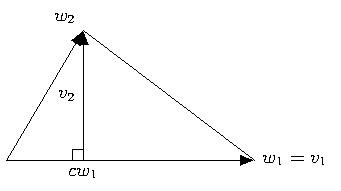
\includegraphics[width=0.5\textwidth]{figuras/gram-schmidt-paso.pdf}
    \end{figure}

    Para encontrar $c$, basta resolver la ecuación
    \begin{equation*}
        0=\iprod{v_2}{w_1}=\iprod{w_2-cw_1}{w_1}=\iprod{w_2}{w_1}-c\iprod{w_1}{w_1}.
    \end{equation*}
    Así,
    \begin{equation*}
        c=\frac{\iprod{w_2}{w_1}}{\norm{w_1}^2}.
    \end{equation*}
    Por tanto,
    \begin{equation*}
        v_2=w_2-\frac{\iprod{w_2}{w_1}}{\norm{w_1}^2}w_1.
    \end{equation*}

    El siguiente teorema muestra que este proceso puede extenderse a cualquier subconjunto linealmente independiente finito.

    \begin{teorema}[Proceso de Gram-Schmidt]
        Sea $V$ un espacio con producto interno y $S=\{w_1,w_2,\dots,w_n\}$ un subconjunto linealmente independiente de $V$. Definamos $S'=\{v_1,v_2,\dots,v_n\}$, donde $v_1=w_1$ y
        \begin{equation*}
            v_k=w_k-\sum_{j=1}^{k-1}\frac{\iprod{w_k}{v_j}}{\norm{v_j}^2}v_j \qquad\text{para } 2\leq k\leq n. \tag{$*$}
        \end{equation*}
        Entonces $S'$ es un conjunto ortogonal de vectores no nulos tal que $\gen{S'}=\gen{S}$.
    \end{teorema}

    \begin{proof}
        Procedemos por inducción sobre $n$, el número de vectores en $S$. Para $k=1,2,\dots,n$, sea $S_k=\{w_1,w_2,\dots,w_k\}$. Si $n=1$, el teorema se cumple tomando $S_1'=S_1$; es decir, $v_1=w_1\neq 0$.

        Supongamos ahora que, para $k-1\geq 1$, el conjunto $S_{k-1}'=\{v_1,v_2,\dots,v_{k-1}\}$ ya fue construido con las propiedades deseadas mediante el uso repetido de ($*$). Mostramos que el conjunto $S_k'=\{v_1,v_2,\dots,v_{k-1},v_k\}$ también tiene las propiedades deseadas, donde $v_k$ se obtiene a partir de $S_{k-1}'$ por ($*$).

        Si $v_k=0$, entonces ($*$) implica que $w_k\in\gen{S_{k-1}'}=\gen{S_{k-1}}$, lo cual contradice que $S_k$ es linealmente independiente. Para $1\leq i\leq k-1$, se sigue de ($*$) que
        \begin{equation*}
            \iprod{v_k}{v_i}=\iprod{w_k}{v_i}-\sum_{j=1}^{k-1}\frac{\iprod{w_k}{v_j}}{\norm{v_j}^2}\iprod{v_j}{v_i}=\iprod{w_k}{v_i}-\frac{\iprod{w_k}{v_i}}{\norm{v_i}^2}\norm{v_i}^2=0,
        \end{equation*}
        pues $\iprod{v_j}{v_i}=0$ si $j\neq i$, por la hipótesis de inducción de que $S_{k-1}'$ es ortogonal. Por tanto $S_k'$ es un conjunto ortogonal de vectores no nulos. Ahora, por ($*$), tenemos que $\gen{S_k'}\subseteq\gen{S_k}$. Pero, por el corolario anterior al teorema anterior, $S_k'$ es linealmente independiente; así, $\dim(\gen{S_k'})=\dim(\gen{S_k}) = k$. Por lo tanto $\gen{S_k'}=\gen{S_k}$.
    \end{proof}

    A la construcción de $\{v_1,v_2,\dots,v_n\}$ mediante el uso del teorema anterior se le llama el \textbf{proceso de Gram-Schmidt}.

    \begin{ejemplo}
        En $\R^4$, sean $w_1=(1,0,1,0)$, $w_2=(1,1,1,1)$ y $w_3=(0,1,2,1)$. Entonces $\{w_1,w_2,w_3\}$ es linealmente independiente. Usamos el proceso de Gram-Schmidt para calcular los vectores ortogonales $v_1$, $v_2$ y $v_3$, y luego normalizamos estos vectores para obtener un conjunto ortonormal.

        Tomamos $v_1=w_1=(1,0,1,0)$. Entonces
        \begin{align*}
            v_2&=w_2-\frac{\iprod{w_2}{v_1}}{\norm{v_1}^2}v_1\\
            &=(1,1,1,1)-\frac{2}{2}(1,0,1,0)\\
            &=(0,1,0,1).
        \end{align*}
        Finalmente,
        \begin{align*}
            v_3&=w_3-\frac{\iprod{w_3}{v_1}}{\norm{v_1}^2}v_1-\frac{\iprod{w_3}{v_2}}{\norm{v_2}^2}v_2\\
            &=(0,1,2,1)-\frac{2}{2}(1,0,1,0)-\frac{2}{2}(0,1,0,1)\\
            &=(-1,0,1,0).
        \end{align*}
        Estos vectores se pueden normalizar para obtener la base ortonormal $\{u_1,u_2,u_3\}$, donde
        \begin{equation*}
            u_1=\frac{1}{\norm{v_1}}v_1=\frac{1}{\sqrt2}(1,0,1,0), \qquad u_2=\frac{1}{\norm{v_2}}v_2=\frac{1}{\sqrt2}(0,1,0,1),
        \end{equation*}
        y
        \begin{equation*}
            u_3=\frac{v_3}{\norm{v_3}}=\frac{1}{\sqrt2}(-1,0,1,0).
        \end{equation*}
    \end{ejemplo}

    \begin{ejemplo}
        Sea $V=P(\R)$ con el producto interno $\iprod{f(x)}{g(x)}=\int_{-1}^{1}f(t)g(t)\,dt$, y consideremos el subespacio $P_2(\R)$ con la base ordenada canónica $\BB$. Usamos el proceso de Gram-Schmidt para sustituir $\BB$ por una base ortogonal $\{v_1,v_2,v_3\}$ de $P_2(\R)$, y luego usamos esta base ortogonal para obtener una base ortonormal de $P_2(\R)$.

        Tomamos $v_1=1$. Entonces $\norm{v_1}^2=\int_{-1}^{1}1^2\,dt=2$, y $\iprod{x}{v_1}=\int_{-1}^{1}t\cdot 1\,dt=0$. Así,
        \begin{equation*}
            v_2=x-\frac{\iprod{x}{v_1}}{\norm{v_1}^2}v_1=x-0=x.
        \end{equation*}
        Además,
        \begin{equation*}
            \iprod{x^2}{v_1}=\int_{-1}^{1}t^2\cdot 1\,dt=\frac{2}{3} \qquad\text{y}\qquad \iprod{x^2}{v_2}=\int_{-1}^{1}t^2\cdot t\,dt=0.
        \end{equation*}
        Por tanto
        \begin{align*}
            v_3&=x^2-\frac{\iprod{x^2}{v_1}}{\norm{v_1}^2}v_1-\frac{\iprod{x^2}{v_2}}{\norm{v_2}^2}v_2\\
            &=x^2-\frac13\cdot 1-0\cdot x\\
            &=x^2-\frac13.
        \end{align*}
        Concluimos que $\{1,x,x^2-\tfrac13\}$ es una base ortogonal de $P_2(\R)$.

        Para obtener una base ortonormal, normalizamos $v_1$, $v_2$ y $v_3$ para obtener
        \begin{equation*}
            u_1=\frac{1}{\sqrt{\int_{-1}^{1}1^2\,dt}}=\frac{1}{\sqrt2}, \qquad u_2=\frac{x}{\sqrt{\int_{-1}^{1}t^2\,dt}}=\sqrt{\frac32}\,x,
        \end{equation*}
        y, análogamente,
        \begin{equation*}
            u_3=\frac{v_3}{\norm{v_3}}=\sqrt{\frac58}\,(3x^2-1).
        \end{equation*}
        Así, $\{u_1,u_2,u_3\}$ es la base ortonormal deseada para $P_2(\R)$.
    \end{ejemplo}

    Si continuamos aplicando el proceso de ortogonalización de Gram-Schmidt a la base $\{1,x,x^2,\dots\}$ de $P(\R)$, obtenemos una base ortogonal cuyos elementos se llaman los \textbf{polinomios de Legendre}. Los polinomios ortogonales $v_1,v_2$ y $v_3$ del ejemplo anterior son los tres primeros polinomios de Legendre.

    El siguiente resultado nos da un método sencillo para representar un vector como combinación lineal de los vectores de una base ortonormal.

    \begin{teorema}
        Sea $V$ un espacio con producto interno no nulo de dimensión finita. Entonces $V$ posee una base ortonormal $\BB$. Más aún, si $\BB=\{v_1,v_2,\dots,v_n\}$ y $x\in V$, entonces
        \begin{equation*}
            x=\sum_{i=1}^{n}\iprod{x}{v_i}v_i.
        \end{equation*}
    \end{teorema}

    \begin{proof}
        Sea $\BB_0$ una base ordenada de $V$. Aplicando el proceso de Gram-Schmidt a $\BB_0$ obtenemos un conjunto ortogonal $\BB'$ de vectores no nulos tal que $\gen{\BB'}=\gen{\BB_0}=V$. Normalizando cada vector de $\BB'$, obtenemos un conjunto ortonormal $\BB$ que genera a $V$. Por el corolario visto al inicio de esta sección, $\BB$ es linealmente independiente; por tanto $\BB$ es una base ortonormal de $V$. El resto del teorema se sigue del corolario al primer teorema de esta sección.
    \end{proof}

    \begin{ejemplo}
        Usamos el teorema anterior para representar el polinomio $f(x)=1+2x+3x^2$ como combinación lineal de los vectores de la base ortonormal $\{u_1,u_2,u_3\}$ de $P_2(\R)$ obtenida en el ejemplo anterior. Observemos que
        \begin{equation*}
            \iprod{f(x)}{u_1}=\int_{-1}^{1}\frac{1}{\sqrt2}(1+2t+3t^2)\,dt=2\sqrt2,
        \end{equation*}
        \begin{equation*}
            \iprod{f(x)}{u_2}=\int_{-1}^{1}\sqrt{\frac32}\,t(1+2t+3t^2)\,dt=\frac{2\sqrt6}{3},
        \end{equation*}
        y
        \begin{equation*}
            \iprod{f(x)}{u_3}=\int_{-1}^{1}\sqrt{\frac58}\,(3t^2-1)(1+2t+3t^2)\,dt=\frac{2\sqrt{10}}{5}.
        \end{equation*}
        Por tanto
        \begin{equation*}
            f(x)=2\sqrt2\,u_1+\frac{2\sqrt6}{3}\,u_2+\frac{2\sqrt{10}}{5}\,u_3.
        \end{equation*}
    \end{ejemplo}

    El teorema anterior también nos da un método sencillo para calcular las entradas de la representación matricial de un operador lineal respecto a una base ortonormal.

    \begin{corolario}
        Sea $V$ un espacio con producto interno de dimensión finita con base ortonormal $\BB=\{v_1,v_2,\dots,v_n\}$. Sea $T$ un operador lineal sobre $V$, y sea $A=[T]_{\BB}$. Entonces, para cualesquiera $i,j$, $A_{ij}=\iprod{T(v_j)}{v_i}$.
    \end{corolario}

    \begin{proof}
        Por el teorema anterior,
        \begin{equation*}
            T(v_j)=\sum_{i=1}^{n}\iprod{T(v_j)}{v_i}v_i.
        \end{equation*}
        Por tanto $A_{ij}=\iprod{T(v_j)}{v_i}$.
    \end{proof}

    Los escalares $\iprod{x}{v_i}$ dados en el teorema anterior se han estudiado extensamente para espacios con producto interno particulares. Aunque los vectores $v_1,v_2,\dots,v_n$ se eligieron de una base ortonormal, introducimos una terminología asociada con conjuntos ortonormales $\BB$ en espacios con producto interno más generales.

    \begin{definicion}[Coeficientes de Fourier]
        Sea $\BB$ un subconjunto ortonormal (posiblemente infinito) de un espacio con producto interno $V$, y sea $x\in V$. Se definen los \textbf{coeficientes de Fourier} de $x$ relativos a $\BB$ como los escalares $\iprod{x}{y}$, donde $y\in\BB$.
    \end{definicion}

    En la primera mitad del siglo XIX, el matemático francés Jean Baptiste Fourier estudió los escalares
    \begin{equation*}
        \int_0^{2\pi}f(t)\sin(nt)\,dt \qquad\text{y}\qquad \int_0^{2\pi}f(t)\cos(nt)\,dt,
    \end{equation*}
    o, más generalmente,
    \begin{equation*}
        c_n=\frac{1}{2\pi}\int_0^{2\pi}f(t)e^{-int}\,dt,
    \end{equation*}
    para una función $f$. En el contexto de un ejemplo de la sección anterior, $c_n=\iprod{f}{f_n}$, donde $f_n(t)=e^{int}$; es decir, $c_n$ es el $n$-ésimo coeficiente de Fourier de una función continua $f\in V$ relativo a $S$. Estos coeficientes son los coeficientes de Fourier \textquotedblleft clásicos\textquotedblright\ de una función, y la literatura sobre ellos es extensa.

    \begin{ejemplo}
        Sea $S=\{e^{int}:n\text{ es un entero}\}$. En un ejemplo de la sección anterior mostramos que $S$ es un conjunto ortonormal en $H$. Calculamos los coeficientes de Fourier de $f(t)=t$ relativos a $S$. Usando integración por partes, tenemos, para $n\neq 0$,
        \begin{equation*}
            \iprod{f}{f_n}=\frac{1}{2\pi}\int_0^{2\pi}t\overline{e^{int}}\,dt=\frac{1}{2\pi}\int_0^{2\pi}te^{-int}\,dt=\frac{-1}{in},
        \end{equation*}
        y, para $n=0$,
        \begin{equation*}
            \iprod{f}{1}=\frac{1}{2\pi}\int_0^{2\pi}t(1)\,dt=\pi.
        \end{equation*}
        Como resultado de estos cálculos, y usando que $\norm{f}^2=\iprod{f}{f}=\frac{4}{3}\pi^2$, obtenemos una cota superior para la suma de una serie infinita particular. En efecto, para cualquier entero $k\geq 1$, el conjunto finito $\{1,f_{-k},\dots,f_{-1},f_1,\dots,f_k\}\subset S$ es ortonormal, así que, por el teorema anterior aplicado al espacio $\gen{\{1,f_{-k},\dots,f_k\}}$ (o, más precisamente, por la desigualdad de Bessel, la cual se sigue de que $0\le \norm*{f-\sum \iprod{f}{y}y}^2$ para cualquier subconjunto ortonormal finito), se tiene
        \begin{align*}
            \norm{f}^2&\geq\sum_{n=-k}^{-1}|\iprod{f}{f_n}|^2+|\iprod{f}{1}|^2+\sum_{n=1}^{k}|\iprod{f}{f_n}|^2\\
            &=\sum_{n=-k}^{-1}\frac{1}{n^2}+\pi^2+\sum_{n=1}^{k}\frac{1}{n^2}=2\sum_{n=1}^{k}\frac{1}{n^2}+\pi^2
        \end{align*}
        para todo $k$. Ahora, usando que $\norm{f}^2=\frac43\pi^2$, obtenemos
        \begin{equation*}
            \frac43\pi^2\geq 2\sum_{n=1}^{k}\frac{1}{n^2}+\pi^2,
        \end{equation*}
        o
        \begin{equation*}
            \frac{\pi^2}{6}\geq\sum_{n=1}^{k}\frac{1}{n^2}.
        \end{equation*}
        Como esta desigualdad vale para todo $k$, podemos hacer $k\to\infty$ para obtener
        \begin{equation*}
            \frac{\pi^2}{6}\geq\sum_{n=1}^{\infty}\frac{1}{n^2}.
        \end{equation*}
        Pueden obtenerse resultados adicionales al reemplazar $f$ por otras funciones.
    \end{ejemplo}

    Estamos ahora listos para introducir el concepto de complemento ortogonal.

    \begin{definicion}[Complemento ortogonal]
        Sea $S$ un subconjunto no vacío de un espacio con producto interno $V$. Se define $S^\perp$ (léase \textquotedblleft $S$ perpendicular\textquotedblright) como el conjunto de todos los vectores de $V$ que son ortogonales a todo vector de $S$; es decir, $S^\perp=\{x\in V:\iprod{x}{y}=0 \text{ para todo } y\in S\}$. Al conjunto $S^\perp$ se le llama el \textbf{complemento ortogonal} de $S$.
    \end{definicion}

    Se ve fácilmente que $S^\perp$ es un subespacio de $V$ para cualquier subconjunto $S$ de $V$: si $x_1,x_2\in S^\perp$, $a\in F$ y $y\in S$, entonces $\iprod{ax_1+x_2}{y}=a\iprod{x_1}{y}+\iprod{x_2}{y}=0$, así que $ax_1+x_2\in S^\perp$; además $0\in S^\perp$ trivialmente.

    \begin{ejemplo}
        Se verifica directamente de la definición que $\{0\}^\perp=V$ (pues todo vector es ortogonal a $0$) y $V^\perp=\{0\}$ (pues si $x\in V^\perp$ entonces $\iprod{x}{x}=0$, y por tanto $x=0$), para cualquier espacio con producto interno $V$.
    \end{ejemplo}

    \begin{ejemplo}
        Si $V=\R^3$ y $S=\{e_3\}$, entonces $S^\perp$ es el plano $xy$.
    \end{ejemplo}

    Consideremos el problema, en $\R^3$, de encontrar la distancia de un punto $P$ a un plano $W$. Problemas de este tipo surgen en muchos contextos. Si $y$ es el vector determinado por $0$ y $P$, podemos replantear el problema así: determinar el vector $u\in W$ que sea \textquotedblleft más cercano\textquotedblright\ a $y$. La distancia buscada está dada claramente por $\norm{y-u}$. Observemos, en la siguiente figura, que el vector $z=y-u$ es ortogonal a todo vector de $W$, y por tanto $z\in W^\perp$.

    \begin{figure}[H]
        \centering
        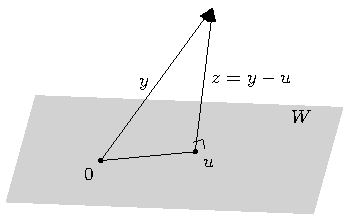
\includegraphics[width=0.5\textwidth]{figuras/distancia-punto-plano.pdf}
    \end{figure}

    El siguiente resultado da un método práctico para encontrar $u$ en el caso en que $W$ es un subespacio de dimensión finita de un espacio con producto interno.

    \begin{teorema}
        Sea $W$ un subespacio de dimensión finita de un espacio con producto interno $V$, y sea $y\in V$. Entonces existen vectores únicos $u\in W$ y $z\in W^\perp$ tales que $y=u+z$. Más aún, si $\{v_1,v_2,\dots,v_k\}$ es una base ortonormal de $W$, entonces
        \begin{equation*}
            u=\sum_{i=1}^{k}\iprod{y}{v_i}v_i.
        \end{equation*}
    \end{teorema}

    \begin{proof}
        Sea $\{v_1,v_2,\dots,v_k\}$ una base ortonormal de $W$, sea $u$ como en la ecuación anterior, y sea $z=y-u$. Claramente $u\in W$ y $y=u+z$.

        Para mostrar que $z\in W^\perp$, basta mostrar que $z$ es ortogonal a cada $v_j$ (pues entonces, para cualquier $w=\sum_{j=1}^k c_jv_j\in W$, se tiene $\iprod{z}{w}=\sum_j \overline{c_j}\iprod{z}{v_j}=0$ por la conjugado-linealidad en la segunda componente, así que $z\in W^\perp$). Para cualquier $j$, tenemos
        \begin{align*}
            \iprod{z}{v_j}&=\iprod{y-\sum_{i=1}^{k}\iprod{y}{v_i}v_i}{v_j}=\iprod{y}{v_j}-\sum_{i=1}^{k}\iprod{y}{v_i}\iprod{v_i}{v_j}\\
            &=\iprod{y}{v_j}-\iprod{y}{v_j}=0.
        \end{align*}

        Para mostrar la unicidad de $u$ y $z$, supongamos que $y=u'+z'$, donde $u'\in W$ y $z'\in W^\perp$. Entonces $u-u'=z'-z\in W\cap W^\perp=\{0\}$. Por tanto $u=u'$ y $z=z'$.
    \end{proof}

    \begin{corolario}
        En la notación del teorema anterior, el vector $u$ es el único vector de $W$ que es \textquotedblleft más cercano\textquotedblright\ a $y$; es decir, para cualquier $x\in W$, $\norm{y-x}\geq\norm{y-u}$, y esta desigualdad es una igualdad si y solo si $x=u$.
    \end{corolario}

    \begin{proof}
        Como en el teorema anterior, tenemos $y=u+z$, donde $z\in W^\perp$. Sea $x\in W$. Entonces $u-x$ es ortogonal a $z$ (pues $u-x\in W$ y $z\in W^\perp$), así que
        \begin{equation*}
            \norm{y-x}^2=\norm{(u-x)+z}^2=\iprod{(u-x)+z}{(u-x)+z}=\norm{u-x}^2+\norm{z}^2
        \end{equation*}
        (usando que $\iprod{u-x}{z}=\iprod{z}{u-x}=0$ por la ortogonalidad)
        \begin{equation*}
            \geq\norm{z}^2=\norm{y-u}^2.
        \end{equation*}
        Supongamos ahora que $\norm{y-x}=\norm{y-u}$. Entonces la desigualdad anterior se convierte en una igualdad, y por tanto $\norm{u-x}^2+\norm{z}^2=\norm{z}^2$; se sigue que $\norm{u-x}=0$, y por tanto $x=u$. El recíproco es evidente.
    \end{proof}

    Al vector $u$ del corolario anterior se le llama la \textbf{proyección ortogonal} de $y$ sobre $W$. Más adelante en este capítulo veremos la importancia de las proyecciones ortogonales de vectores en la aplicación a mínimos cuadrados.

    \begin{ejemplo}
        Sea $V=P_3(\R)$ con el producto interno $\iprod{f(x)}{g(x)}=\int_{-1}^{1}f(t)g(t)\,dt$ para todos $f(x),g(x)\in V$. Calculamos la proyección ortogonal $f_1(x)$ de $f(x)=x^3$ sobre $P_2(\R)$.

        Por un ejemplo anterior, $\{u_1,u_2,u_3\}=\left\{\frac{1}{\sqrt2},\sqrt{\frac32}\,x,\sqrt{\frac58}\,(3x^2-1)\right\}$ es una base ortonormal de $P_2(\R)$. Para estos vectores, tenemos
        \begin{equation*}
            \iprod{f(x)}{u_1}=\int_{-1}^{1}t^3\frac{1}{\sqrt2}\,dt=0, \qquad \iprod{f(x)}{u_2}=\int_{-1}^{1}t^3\sqrt{\frac32}\,t\,dt=\frac{\sqrt6}{5},
        \end{equation*}
        y
        \begin{equation*}
            \iprod{f(x)}{u_3}=\int_{-1}^{1}t^3\sqrt{\frac58}\,(3t^2-1)\,dt=0.
        \end{equation*}
        Por tanto
        \begin{equation*}
            f_1(x)=\iprod{f(x)}{u_1}u_1+\iprod{f(x)}{u_2}u_2+\iprod{f(x)}{u_3}u_3=\frac{3}{5}x.
        \end{equation*}
    \end{ejemplo}

    En un curso anterior se mostró que todo conjunto linealmente independiente en un espacio vectorial de dimensión finita puede extenderse a una base. El siguiente teorema proporciona un análogo interesante para un subconjunto ortonormal de un espacio con producto interno de dimensión finita.

    \begin{teorema}
        Supongamos que $S=\{v_1,v_2,\dots,v_k\}$ es un conjunto ortonormal en un espacio con producto interno $V$ de dimensión $n$. Entonces:
        \begin{enumerate}[label=(\alph*)]
            \item $S$ puede extenderse a una base ortonormal $\{v_1,v_2,\dots,v_k,v_{k+1},\dots,v_n\}$ de $V$.
            \item Si $W=\gen{S}$, entonces $S_1=\{v_{k+1},v_{k+2},\dots,v_n\}$ (con la notación anterior) es una base ortonormal de $W^\perp$.
            \item Si $W$ es cualquier subespacio de $V$, entonces $\dim(V)=\dim(W)+\dim(W^\perp)$.
        \end{enumerate}
    \end{teorema}

    \begin{proof}
        (a) Como $S$ es linealmente independiente (por ser un conjunto ortogonal de vectores no nulos), puede extenderse a una base ordenada $S'=\{v_1,v_2,\dots,v_k,w_{k+1},\dots,w_n\}$ de $V$ (por el teorema de extensión a una base, ya visto en el primer curso). Apliquemos ahora el proceso de Gram-Schmidt a $S'$. Los primeros $k$ vectores resultantes de este proceso son los vectores de $S$ (pues, al ser ya ortonormales, el proceso los deja sin cambio, ya que en la fórmula $(*)$ cada resta es cero), y este nuevo conjunto genera a $V$. Normalizando los últimos $n-k$ vectores de este conjunto se produce un conjunto ortonormal que genera a $V$. El resultado se sigue.

        (b) Como $S_1$ es un subconjunto de la base de (a), es linealmente independiente. Como $S_1$ es claramente un subconjunto de $W^\perp$, basta mostrar que genera a $W^\perp$. Notemos que, para cualquier $x\in V$, tenemos, por el teorema anterior,
        \begin{equation*}
            x=\sum_{i=1}^{n}\iprod{x}{v_i}v_i.
        \end{equation*}
        Si $x\in W^\perp$, entonces $\iprod{x}{v_i}=0$ para $1\leq i\leq k$. Por lo tanto,
        \begin{equation*}
            x=\sum_{i=k+1}^{n}\iprod{x}{v_i}v_i\in\gen{S_1}.
        \end{equation*}

        (c) Sea $W$ un subespacio de $V$. Es un espacio con producto interno de dimensión finita porque $V$ lo es, y por tanto posee una base ortonormal $\{v_1,\dots,v_k\}$. Por (a) y (b), tenemos $\dim(V)=n=k+(n-k)=\dim(W)+\dim(W^\perp)$.
    \end{proof}

    \begin{ejemplo}
        Sea $W=\gen{\{e_1,e_2\}}$ en $F^3$. Entonces $x=(a,b,c)\in W^\perp$ si y solo si $0=\iprod{x}{e_1}=a$ y $0=\iprod{x}{e_2}=b$. Así $x=(0,0,c)$, y por tanto $W^\perp=\gen{\{e_3\}}$. Podemos deducir el mismo resultado observando que $e_3\in W^\perp$ y, por (c), que $\dim(W^\perp)=3-2=1$.
    \end{ejemplo}

    \section{El adjunto de un operador lineal}

    En la Sección~6.1 definimos la transpuesta conjugada (o matriz adjunta) $A^*$ de una matriz $A$. Para un operador lineal $T$ sobre un espacio con producto interno $V$, definimos ahora un operador lineal relacionado sobre $V$, llamado el \textit{adjunto} de $T$, cuya representación matricial respecto a cualquier base ortonormal $\BB$ de $V$ es $[T]_{\BB}^*$. La analogía entre la conjugación de números complejos y los adjuntos de operadores lineales se hará evidente. Primero necesitamos un resultado preliminar.

    Sea $V$ un espacio con producto interno, y sea $y\in V$. La función $g:V\to F$ definida por $g(x)=\iprod{x}{y}$ es claramente lineal. Más interesante aún es el hecho de que, si $V$ es de dimensión finita, toda transformación lineal de $V$ en $F$ es de esta forma.

    \begin{teorema}
        Sea $V$ un espacio con producto interno de dimensión finita sobre $F$, y sea $g:V\to F$ una transformación lineal. Entonces existe un único vector $y\in V$ tal que $g(x)=\iprod{x}{y}$ para todo $x\in V$.
    \end{teorema}

    \begin{proof}
        Sea $\BB=\{v_1,v_2,\dots,v_n\}$ una base ortonormal de $V$, y sea
        \begin{equation*}
            y=\sum_{i=1}^{n}\overline{g(v_i)}v_i.
        \end{equation*}
        Definamos $h:V\to F$ por $h(x)=\iprod{x}{y}$, que es claramente lineal. Además, para $1\leq j\leq n$,
        \begin{equation*}
            h(v_j)=\iprod{v_j}{\sum_{i=1}^{n}\overline{g(v_i)}v_i}=\sum_{i=1}^{n}g(v_i)\iprod{v_j}{v_i}=\sum_{i=1}^{n}g(v_i)\delta_{ji}=g(v_j).
        \end{equation*}
        Como $g$ y $h$ coinciden en $\BB$, tenemos $g=h$ (dos transformaciones lineales que coinciden en una base son iguales, como se vio en el primer curso).

        Para mostrar que $y$ es único, supongamos que $g(x)=\iprod{x}{y'}$ para todo $x$. Entonces $\iprod{x}{y}=\iprod{x}{y'}$ para todo $x$; así, por una propiedad ya establecida en la Sección~6.1, $y=y'$.
    \end{proof}

    \begin{ejemplo}
        Definamos $g:\R^2\to\R$ por $g(a_1,a_2)=2a_1+a_2$; claramente $g$ es una transformación lineal. Sea $\BB=\{e_1,e_2\}$, y sea $y=g(e_1)e_1+g(e_2)e_2=2e_1+e_2=(2,1)$, como en la demostración del teorema anterior. Entonces $g(a_1,a_2)=\iprod{(a_1,a_2)}{(2,1)}=2a_1+a_2$.
    \end{ejemplo}

    \begin{teorema}
        Sea $V$ un espacio con producto interno de dimensión finita, y sea $T$ un operador lineal sobre $V$. Entonces existe una única función $T^*:V\to V$ tal que $\iprod{T(x)}{y}=\iprod{x}{T^*(y)}$ para todos $x,y\in V$. Más aún, $T^*$ es lineal.
    \end{teorema}

    \begin{proof}
        Sea $y\in V$. Definamos $g:V\to F$ por $g(x)=\iprod{T(x)}{y}$ para todo $x\in V$. Mostramos primero que $g$ es lineal. Sean $x_1,x_2\in V$ y $c\in F$. Entonces
        \begin{align*}
            g(cx_1+x_2)&=\iprod{T(cx_1+x_2)}{y}=\iprod{cT(x_1)+T(x_2)}{y}\\
            &=c\iprod{T(x_1)}{y}+\iprod{T(x_2)}{y}=cg(x_1)+g(x_2).
        \end{align*}
        Así, $g$ es lineal.

        Aplicamos ahora el teorema anterior para obtener un único vector $y'\in V$ tal que $g(x)=\iprod{x}{y'}$ para todo $x\in V$; es decir, $\iprod{T(x)}{y}=\iprod{x}{y'}$ para todo $x\in V$. Definiendo $T^*:V\to V$ por $T^*(y)=y'$, tenemos $\iprod{T(x)}{y}=\iprod{x}{T^*(y)}$.

        Para mostrar que $T^*$ es lineal, sean $y_1,y_2\in V$ y $c\in F$. Entonces, para cualquier $x\in V$,
        \begin{align*}
            \iprod{x}{T^*(cy_1+y_2)}&=\iprod{T(x)}{cy_1+y_2}=\overline{c}\iprod{T(x)}{y_1}+\iprod{T(x)}{y_2}\\
            &=\overline{c}\iprod{x}{T^*(y_1)}+\iprod{x}{T^*(y_2)}=\iprod{x}{cT^*(y_1)+T^*(y_2)}.
        \end{align*}
        Como $x$ es arbitrario, $T^*(cy_1+y_2)=cT^*(y_1)+T^*(y_2)$ por una propiedad ya establecida en la Sección~6.1.

        Finalmente, mostramos que $T^*$ es único. Supongamos que $U:V\to V$ es lineal y satisface $\iprod{T(x)}{y}=\iprod{x}{U(y)}$ para todos $x,y\in V$. Entonces $\iprod{x}{T^*(y)}=\iprod{x}{U(y)}$ para todos $x,y\in V$, así que $T^*=U$.
    \end{proof}

    Al operador lineal $T^*$ descrito en el teorema anterior se le llama el \textbf{adjunto} del operador $T$. El símbolo $T^*$ se lee \textquotedblleft $T$ estrella\textquotedblright.

    Así, $T^*$ es el único operador sobre $V$ que satisface $\iprod{T(x)}{y}=\iprod{x}{T^*(y)}$ para todos $x,y\in V$. Notemos también que
    \begin{equation*}
        \iprod{x}{T(y)}=\overline{\iprod{T(y)}{x}}=\overline{\iprod{y}{T^*(x)}}=\iprod{T^*(x)}{y};
    \end{equation*}
    así, $\iprod{x}{T(y)}=\iprod{T^*(x)}{y}$ para todos $x,y\in V$. Podemos ver estas ecuaciones simbólicamente como agregar un $*$ a $T$ al desplazar su posición dentro del símbolo de producto interno.

    Para un espacio con producto interno de dimensión infinita, el adjunto de un operador lineal $T$ puede definirse como la función $T^*$ tal que $\iprod{T(x)}{y}=\iprod{x}{T^*(y)}$ para todos $x,y\in V$, siempre que exista. Aunque la unicidad y la linealidad de $T^*$ se siguen como antes, la existencia del adjunto no está garantizada en general. El lector debe notar la necesidad de la hipótesis de dimensión finita en la demostración del primer teorema de esta sección. Muchos de los teoremas que probamos sobre adjuntos, sin embargo, no dependen de que $V$ sea de dimensión finita. Así, a menos que se indique lo contrario, adoptamos la convención de que, en el resto de este capítulo, una referencia al adjunto de un operador lineal sobre un espacio con producto interno de dimensión infinita supone su existencia.

    El siguiente teorema es útil para calcular adjuntos.

    \begin{teorema}
        Sea $V$ un espacio con producto interno de dimensión finita, y sea $\BB$ una base ortonormal de $V$. Si $T$ es un operador lineal sobre $V$, entonces
        \begin{equation*}
            [T^*]_{\BB}=[T]_{\BB}^*.
        \end{equation*}
    \end{teorema}

    \begin{proof}
        Sean $A=[T]_{\BB}$, $B=[T^*]_{\BB}$ y $\BB=\{v_1,v_2,\dots,v_n\}$. Entonces, por el corolario visto en la Sección~6.2,
        \begin{equation*}
            B_{ij}=\iprod{T^*(v_j)}{v_i}=\overline{\iprod{v_i}{T^*(v_j)}}=\overline{\iprod{T(v_i)}{v_j}}=\overline{A_{ji}}=(A^*)_{ij}.
        \end{equation*}
        Por tanto $B=A^*$.
    \end{proof}

    \begin{corolario}
        Sea $A$ una matriz $n\times n$. Entonces $L_{A^*}=(L_A)^*$.
    \end{corolario}

    \begin{proof}
        Sea $\BB$ la base canónica ordenada de $F^n$, la cual es ortonormal respecto al producto interno estándar. Como $[L_A]_{\BB}=A$ (un hecho ya establecido en el primer curso), tenemos, por el teorema anterior, $[(L_A)^*]_{\BB}=[L_A]_{\BB}^*=A^*$. Así $[(L_A)^*]_{\BB}=[L_{A^*}]_{\BB}=A^*$, y por tanto $(L_A)^*=L_{A^*}$.
    \end{proof}

    Como ilustración del teorema anterior, calculamos el adjunto de un operador lineal específico.

    \begin{ejemplo}
        Sea $T$ el operador lineal sobre $\C^2$ definido por $T(a_1,a_2)=(2ia_1+3a_2,a_1-a_2)$. Si $\BB$ es la base canónica ordenada de $\C^2$, entonces
        \begin{equation*}
            [T]_{\BB}=\begin{pmatrix}2i&3\\1&-1\end{pmatrix}.
        \end{equation*}
        Así,
        \begin{equation*}
            [T^*]_{\BB}=[T]_{\BB}^*=\begin{pmatrix}-2i&1\\3&-1\end{pmatrix}.
        \end{equation*}
        Por tanto $T^*(a_1,a_2)=(-2ia_1+a_2,3a_1-a_2)$.
    \end{ejemplo}

    El siguiente teorema sugiere una analogía entre la conjugación de números complejos y los adjuntos de operadores lineales.

    \begin{teorema}
        Sea $V$ un espacio con producto interno, y sean $T$ y $U$ operadores lineales sobre $V$. Entonces:
        \begin{enumerate}[label=(\alph*)]
            \item $(T+U)^*=T^*+U^*$;
            \item $(cT)^*=\overline{c}T^*$ para cualquier $c\in F$;
            \item $(TU)^*=U^*T^*$;
            \item $T^{**}=T$;
            \item $I^*=I$.
        \end{enumerate}
    \end{teorema}

    \begin{proof}
        Sean $x,y\in V$.

        (a) Como
        \begin{align*}
            \iprod{x}{(T+U)^*(y)}&=\iprod{(T+U)(x)}{y}=\iprod{T(x)+U(x)}{y}\\
            &=\iprod{T(x)}{y}+\iprod{U(x)}{y}=\iprod{x}{T^*(y)}+\iprod{x}{U^*(y)}=\iprod{x}{(T^*+U^*)(y)},
        \end{align*}
        $T^*+U^*$ tiene la propiedad que caracteriza a $(T+U)^*$ de forma única. Por tanto $T^*+U^*=(T+U)^*$.

        (b) Como
        \begin{align*}
            \iprod{x}{(cT)^*(y)}=\iprod{(cT)(x)}{y}=c\iprod{T(x)}{y}=c\iprod{x}{T^*(y)}=\iprod{x}{\overline{c}T^*(y)},
        \end{align*}
        (usando, en el último paso, que el producto interno es conjugado lineal en la segunda componente), $\overline{c}T^*$ tiene la propiedad que caracteriza a $(cT)^*$. Así $(cT)^*=\overline{c}T^*$.

        (c) Como
        \begin{equation*}
            \iprod{x}{(TU)^*(y)}=\iprod{(TU)(x)}{y}=\iprod{T(U(x))}{y}=\iprod{U(x)}{T^*(y)}=\iprod{x}{U^*(T^*(y))}=\iprod{x}{(U^*T^*)(y)},
        \end{equation*}
        $U^*T^*$ tiene la propiedad que caracteriza a $(TU)^*$. Así $(TU)^*=U^*T^*$.

        (d) Análogamente, como
        \begin{equation*}
            \iprod{T(x)}{y}=\iprod{x}{T^*(y)}=\overline{\iprod{T^*(y)}{x}}=\overline{\iprod{y}{T^{**}(x)}}=\iprod{T^{**}(x)}{y},
        \end{equation*}
        se sigue (usando que $x,y$ son arbitrarios y la unicidad del adjunto) que $T^{**}=T$.

        (e) Como $\iprod{I(x)}{y}=\iprod{x}{y}=\iprod{x}{I(y)}$, $I$ tiene la propiedad que caracteriza a $I^*$. Así $I^*=I$.
    \end{proof}

    La misma demostración funciona en el caso de dimensión infinita, siempre que se suponga la existencia de $T^*$ y $U^*$.

    \begin{corolario}
        Sean $A$ y $B$ matrices $n\times n$. Entonces:
        \begin{enumerate}[label=(\alph*)]
            \item $(A+B)^*=A^*+B^*$;
            \item $(cA)^*=\overline{c}A^*$ para todo $c\in F$;
            \item $(AB)^*=B^*A^*$;
            \item $A^{**}=A$;
            \item $I^*=I$.
        \end{enumerate}
    \end{corolario}

    \begin{proof}
        Probamos (c); las demás partes se prueban de manera análoga a partir de la definición de matriz adjunta, $(X^*)_{ij}=\overline{X_{ji}}$.

        Para (c): como $L_{(AB)^*}=(L_{AB})^*=(L_AL_B)^*=(L_B)^*(L_A)^*=L_{B^*}L_{A^*}=L_{B^*A^*}$, tenemos $(AB)^*=B^*A^*$.

        Para (a): $((A+B)^*)_{ij}=\overline{(A+B)_{ji}}=\overline{A_{ji}}+\overline{B_{ji}}=(A^*)_{ij}+(B^*)_{ij}=(A^*+B^*)_{ij}$, así que $(A+B)^*=A^*+B^*$.

        Para (b): $((cA)^*)_{ij}=\overline{(cA)_{ji}}=\overline{c}\,\overline{A_{ji}}=\overline{c}(A^*)_{ij}$, así que $(cA)^*=\overline{c}A^*$.

        Para (d): $((A^*)^*)_{ij}=\overline{(A^*)_{ji}}=\overline{\overline{A_{ij}}}=A_{ij}$, así que $A^{**}=A$.

        Para (e): $(I^*)_{ij}=\overline{I_{ji}}=\overline{\delta_{ji}}=\delta_{ij}=I_{ij}$ (pues $\delta_{ji}$ es real), así que $I^*=I$.
    \end{proof}

    En la demostración anterior de (c), nos apoyamos en el corolario visto anteriormente en esta sección ($L_{A^*}=(L_A)^*$). Una demostración alternativa, válida incluso para matrices no cuadradas, puede darse apelando directamente a la definición de la transpuesta conjugada de una matriz.

    \subsection*{Aproximación por mínimos cuadrados}

    Consideremos el siguiente problema: un experimentador recolecta datos tomando mediciones $y_1,y_2,\dots,y_m$ en los tiempos $t_1,t_2,\dots,t_m$, respectivamente. Por ejemplo, podría estar midiendo el desempleo en varios momentos durante cierto periodo. Supongamos que los datos $(t_1,y_1),(t_2,y_2),\dots,(t_m,y_m)$ se grafican como puntos en el plano. (Véase la siguiente figura.) A partir de esta gráfica, el experimentador percibe que existe una relación esencialmente lineal entre $y$ y $t$, digamos $y=ct+d$, y quisiera encontrar las constantes $c$ y $d$ tales que la recta $y=ct+d$ represente el mejor ajuste posible a los datos recolectados. Una estimación de dicho ajuste consiste en calcular el error $E$, que representa la suma de los cuadrados de las distancias verticales de los puntos a la recta; es decir,
    \begin{equation*}
        E=\sum_{i=1}^{m}(y_i-ct_i-d)^2.
    \end{equation*}

    \begin{figure}[H]
        \centering
        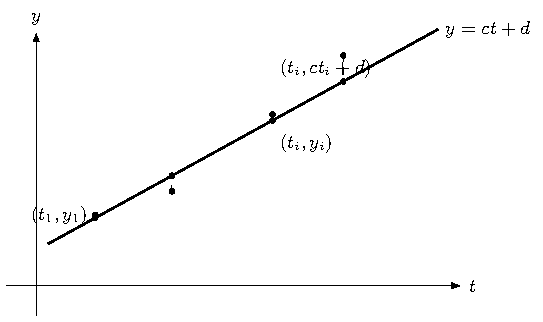
\includegraphics[width=0.75\textwidth]{figuras/6-3-minimos-cuadrados.pdf}
    \end{figure}

    Así, el problema se reduce a encontrar las constantes $c$ y $d$ que minimicen $E$. (Por esta razón, a la recta $y=ct+d$ se le llama la \textbf{recta de mínimos cuadrados}.) Si tomamos
    \begin{equation*}
        A=\begin{pmatrix}t_1&1\\t_2&1\\\vdots&\vdots\\t_m&1\end{pmatrix}, \qquad x=\begin{pmatrix}c\\d\end{pmatrix}, \qquad\text{y}\qquad y=\begin{pmatrix}y_1\\y_2\\\vdots\\y_m\end{pmatrix},
    \end{equation*}
    entonces se sigue que $E=\norm{y-Ax}^2$.

    Desarrollamos un método general para encontrar explícitamente un vector $x_0\in F^n$ que minimice $E$; es decir, dada una matriz $A\in M_{m\times n}(F)$, encontramos $x_0\in F^n$ tal que $\norm{y-Ax_0}\leq\norm{y-Ax}$ para todo $x\in F^n$. Este método no solo nos permite encontrar la función lineal que mejor se ajusta a los datos, sino también, para cualquier entero positivo $n$, el mejor ajuste usando un polinomio de grado a lo más $n$.

    Primero necesitamos algo de notación y dos lemas sencillos. Para $x,y\in F^n$, sea $\iprod{x}{y}_n$ el producto interno estándar de $x$ y $y$ en $F^n$. Recordemos que, si $x$ y $y$ se ven como vectores columna, entonces $\iprod{x}{y}_n=y^*x$.

    \begin{lema}
        Sea $A\in M_{m\times n}(F)$, $x\in F^n$ y $y\in F^m$. Entonces
        \begin{equation*}
            \iprod{Ax}{y}_m=\iprod{x}{A^*y}_n.
        \end{equation*}
    \end{lema}

    \begin{proof}
        Viendo a $x$ y $y$ como vectores columna,
        \begin{equation*}
            \iprod{Ax}{y}_m=y^*(Ax)=(y^*A)x=(A^*y)^*x=\iprod{x}{A^*y}_n,
        \end{equation*}
        donde usamos que $(y^*A)=(A^*y)^*$, pues $(A^*y)^*=y^*A^{**}=y^*A$ (usando que $A^{**}=A$).
    \end{proof}

    \begin{lema}
        Sea $A\in M_{m\times n}(F)$. Entonces $\rg(A^*A)=\rg(A)$.
    \end{lema}

    \begin{proof}
        Por el teorema de la dimensión, basta mostrar que, para $x\in F^n$, $A^*Ax=0$ si y solo si $Ax=0$. Claramente $Ax=0$ implica $A^*Ax=0$. Supongamos entonces que $A^*Ax=0$. Entonces
        \begin{equation*}
            0=\iprod{A^*Ax}{x}_n=\iprod{Ax}{Ax}_m,
        \end{equation*}
        de modo que $Ax=0$.
    \end{proof}

    \begin{corolario}
        Si $A$ es una matriz $m\times n$ tal que $\rg(A)=n$, entonces $A^*A$ es invertible.
    \end{corolario}

    Sea ahora $A$ una matriz $m\times n$ y $y\in F^m$. Definamos $W=\{Ax:x\in F^n\}$; es decir, $W=\Im(L_A)$. Por el corolario visto en la Sección~6.2, existe un único vector en $W$ más cercano a $y$. Llamemos a este vector $Ax_0$, donde $x_0\in F^n$. Entonces $\norm{Ax_0-y}\leq\norm{Ax-y}$ para todo $x\in F^n$; así, $x_0$ tiene la propiedad de que $E=\norm{Ax_0-y}$ es mínima.

    Para desarrollar un método práctico para encontrar tal $x_0$, notamos, por el teorema y su corolario vistos en la Sección~6.2, que $Ax_0-y\in W^\perp$; así, $\iprod{Ax}{Ax_0-y}_m=0$ para todo $x\in F^n$. Por el primer lema anterior, tenemos entonces que $\iprod{x}{A^*(Ax_0-y)}_n=0$ para todo $x\in F^n$; es decir, que $A^*(Ax_0-y)=0$. Así que necesitamos únicamente encontrar una solución $x_0$ a $A^*Ax_0=A^*y$. Si, además, suponemos que $\rg(A)=n$, entonces, por el segundo lema anterior, tenemos $x_0=(A^*A)^{-1}A^*y$. Resumimos esta discusión en el siguiente teorema.

    \begin{teorema}
        Sea $A\in M_{m\times n}(F)$ y $y\in F^m$. Entonces existe $x_0\in F^n$ tal que $(A^*A)x_0=A^*y$ y $\norm{Ax_0-y}\leq\norm{Ax-y}$ para todo $x\in F^n$. Más aún, si $\rg(A)=n$, entonces $x_0=(A^*A)^{-1}A^*y$.
    \end{teorema}

    Volviendo a nuestro experimentador, supongamos que los datos recolectados son $(1,2),(2,3),(3,5)$ y $(4,7)$. Entonces
    \begin{equation*}
        A=\begin{pmatrix}1&1\\2&1\\3&1\\4&1\end{pmatrix} \qquad\text{y}\qquad y=\begin{pmatrix}2\\3\\5\\7\end{pmatrix};
    \end{equation*}
    por tanto
    \begin{equation*}
        A^*A=\begin{pmatrix}1&2&3&4\\1&1&1&1\end{pmatrix}\begin{pmatrix}1&1\\2&1\\3&1\\4&1\end{pmatrix}=\begin{pmatrix}30&10\\10&4\end{pmatrix}.
    \end{equation*}
    Así,
    \begin{equation*}
        (A^*A)^{-1}=\frac{1}{20}\begin{pmatrix}4&-10\\-10&30\end{pmatrix}.
    \end{equation*}
    Por tanto
    \begin{equation*}
        \begin{pmatrix}c\\d\end{pmatrix}=x_0=\frac{1}{20}\begin{pmatrix}4&-10\\-10&30\end{pmatrix}\begin{pmatrix}1&2&3&4\\1&1&1&1\end{pmatrix}\begin{pmatrix}2\\3\\5\\7\end{pmatrix}=\begin{pmatrix}1.7\\0\end{pmatrix}.
    \end{equation*}
    Se sigue que la recta $y=1.7t$ es la recta de mínimos cuadrados. El error $E$ puede calcularse directamente como $\norm{Ax_0-y}^2=0.3$.

    Supongamos que el experimentador hubiera elegido los tiempos $t_i$ ($1\leq i\leq m$) de modo que satisficieran $\sum_{i=1}^{m}t_i=0$. Entonces las dos columnas de $A$ serían ortogonales, así que $A^*A$ sería una matriz diagonal, y en tal caso los cálculos se simplifican considerablemente.

    En la práctica, la matriz $A$ de tamaño $m\times 2$ de nuestra aplicación de mínimos cuadrados tiene rango igual a dos, y por tanto $A^*A$ es invertible por el corolario visto anteriormente. Pues, de lo contrario, la primera columna de $A$ sería un múltiplo de la segunda, que consiste enteramente de unos; pero esto ocurriría únicamente si el experimentador recolectara todos los datos en un mismo instante.

    Finalmente, el método anterior también puede aplicarse si, para alguna $k$, el experimentador desea ajustar a los datos un polinomio $y=ct^2+dt+e$ de grado a lo más $2$. Por ejemplo, si se desea un polinomio de grado a lo más $2$, el modelo apropiado es
    \begin{equation*}
        x=\begin{pmatrix}c\\d\\e\end{pmatrix}, \qquad y=\begin{pmatrix}y_1\\y_2\\\vdots\\y_m\end{pmatrix}, \qquad\text{y}\qquad A=\begin{pmatrix}t_1^2&t_1&1\\\vdots&\vdots&\vdots\\t_m^2&t_m&1\end{pmatrix}.
    \end{equation*}

    \subsection*{Soluciones mínimas de sistemas de ecuaciones lineales}

    Incluso cuando un sistema de ecuaciones lineales $Ax=b$ es consistente, puede no haber una solución única. En tales casos, puede ser deseable encontrar una solución de norma mínima. Una solución $s$ a $Ax=b$ se llama una \textbf{solución mínima} si $\norm{s}\leq\norm{u}$ para cualquier otra solución $u$. El siguiente teorema asegura que todo sistema consistente de ecuaciones lineales tiene una única solución mínima, y proporciona un método para calcularla.

    \begin{teorema}
        Sea $A\in M_{m\times n}(F)$ y $b\in F^m$. Supongamos que $Ax=b$ es consistente. Entonces se cumple lo siguiente:
        \begin{enumerate}[label=(\alph*)]
            \item Existe exactamente una solución mínima $s$ de $Ax=b$, y $s\in\Im(L_{A^*})$.
            \item El vector $s$ es la única solución de $Ax=b$ que se encuentra en $\Im(L_{A^*})$; es decir, si $u$ satisface $(AA^*)u=b$, entonces $s=A^*u$.
        \end{enumerate}
    \end{teorema}

    \begin{proof}
        (a) Por simplicidad de notación, sean $W=\Im(L_{A^*})$ y $W'=\ker(L_A)$. Mostramos primero que $W^\perp=W'$: para $x\in F^n$,
        \begin{equation*}
            x\in W^\perp \iff \iprod{x}{A^*y}_n=0 \ \forall y\in F^m \iff \iprod{Ax}{y}_m=0 \ \forall y\in F^m \iff Ax=0 \iff x\in W',
        \end{equation*}
        donde la penúltima equivalencia se obtiene tomando $y=Ax$ (que da $\norm{Ax}^2=0$, luego $Ax=0$) para una dirección, y es inmediata para la otra; y usamos el primer lema de esta sección para la primera equivalencia.

        Sea $x$ cualquier solución de $Ax=b$. Por el teorema visto en la Sección~6.2, $x=s+y$ para algún $s\in W$ y $y\in W^\perp=W'$. Como $Ay=0$, tenemos $b=Ax=As+Ay=As$. Así, $s$ es una solución de $Ax=b$ que se encuentra en $W$.

        Para probar (a), basta mostrar que $s$ es la única solución mínima. Sea $v$ cualquier otra solución de $Ax=b$. Como en un curso anterior, se tiene $v=s+u$, donde $u\in W'$. Como $s\in W$, que es igual a $(W')^\perp$, tenemos, usando que $s\perp u$ (Pitágoras en espacios con producto interno: si $\iprod{s}{u}=0$, entonces $\norm{s+u}^2=\norm{s}^2+2\Re\iprod{s}{u}+\norm{u}^2=\norm{s}^2+\norm{u}^2$),
        \begin{equation*}
            \norm{v}^2=\norm{s+u}^2=\norm{s}^2+\norm{u}^2\geq\norm{s}^2.
        \end{equation*}
        Así $s$ es una solución mínima. También vemos, del cálculo anterior, que si $\norm{v}=\norm{s}$, entonces $u=0$; por tanto $v=s$. Así, $s$ es la única solución mínima de $Ax=b$, lo cual prueba (a).

        (b) Supongamos que $v$ es también una solución de $Ax=b$ que se encuentra en $W$. Entonces
        \begin{equation*}
            v-s\in W\cap W'=W\cap W^\perp=\{0\};
        \end{equation*}
        así $v=s$.

        Finalmente, supongamos que $(AA^*)u=b$, y sea $v=A^*u$. Entonces $v\in W$ y $Av=b$. Por tanto $s=v=A^*u$ por lo probado anteriormente.
    \end{proof}

    \begin{ejemplo}
        Consideremos el sistema
        \begin{align*}
            x+2y+z&=4\\
            x-y+2z&=-11\\
            x+5y&=19.
        \end{align*}
        Sean
        \begin{equation*}
            A=\begin{pmatrix}1&2&1\\1&-1&2\\1&5&0\end{pmatrix} \qquad\text{y}\qquad b=\begin{pmatrix}4\\-11\\19\end{pmatrix}.
        \end{equation*}
        Para encontrar la solución mínima a este sistema, primero debemos encontrar alguna solución $u$ de $AA^*x=b$. Ahora
        \begin{equation*}
            AA^*=\begin{pmatrix}6&1&11\\1&6&-4\\11&-4&26\end{pmatrix};
        \end{equation*}
        así que consideramos el sistema
        \begin{align*}
            6x+y+11z&=4\\
            x+6y-4z&=-11\\
            11x-4y+26z&=19,
        \end{align*}
        para el cual una solución es
        \begin{equation*}
            u=\begin{pmatrix}1\\-2\\0\end{pmatrix}.
        \end{equation*}
        (Cualquier solución basta.) Por tanto
        \begin{equation*}
            s=A^*u=\begin{pmatrix}-1\\4\\-3\end{pmatrix}
        \end{equation*}
        es la solución mínima del sistema dado.
    \end{ejemplo}

    \section{Operadores normales y autoadjuntos}

    Hemos visto la importancia de los operadores diagonalizables en el Capítulo~1. Para estos operadores, es necesario y suficiente que el espacio vectorial $V$ posea una base de vectores propios. Como $V$ es, en este capítulo, un espacio con producto interno, es razonable buscar condiciones que garanticen que $V$ tenga una base \textit{ortonormal} de vectores propios. Un resultado muy importante que nos ayuda a lograr este objetivo es el teorema de Schur. La formulación que sigue está en términos de operadores lineales; la siguiente sección contiene la versión matricial, más familiar. Comenzamos con un lema.

    \begin{lema}
        Sea $T$ un operador lineal sobre un espacio con producto interno de dimensión finita $V$. Si $T$ tiene un vector propio, entonces también lo tiene $T^*$.
    \end{lema}

    \begin{proof}
        Supongamos que $v$ es un vector propio de $T$ con valor propio correspondiente $\lambda$. Entonces, para cualquier $x\in V$,
        \begin{equation*}
            0=\iprod{0}{x}=\iprod{(T-\lambda I)(v)}{x}=\iprod{v}{(T-\lambda I)^*(x)}=\iprod{v}{(T^*-\overline{\lambda}I)(x)},
        \end{equation*}
        y por tanto $v$ es ortogonal a la imagen de $T^*-\overline{\lambda}I$. Así, $T^*-\overline{\lambda}I$ no es sobreyectiva, y por tanto tampoco es inyectiva. Así, $T^*-\overline{\lambda}I$ tiene espacio nulo no nulo, y cualquier vector no nulo de este espacio nulo es un vector propio de $T^*$ con valor propio correspondiente $\overline{\lambda}$.
    \end{proof}

    Recordemos (véase el Capítulo~1) que un subespacio $W$ de $V$ se dice \textbf{$T$-invariante} si $T(W)$ está contenido en $W$. Si $W$ es $T$-invariante, podemos definir la restricción $T_W:W\to W$ por $T_W(x)=T(x)$ para todo $x\in W$. Es claro que $T_W$ es un operador lineal sobre $W$.

    \begin{teorema}[Schur]
        Sea $T$ un operador lineal sobre un espacio con producto interno de dimensión finita $V$. Supongamos que el polinomio característico de $T$ se escinde. Entonces existe una base ortonormal $\BB$ de $V$ tal que la matriz $[T]_{\BB}$ es triangular superior.
    \end{teorema}

    \begin{proof}
        Procedemos por inducción sobre la dimensión $n$ de $V$. El resultado es inmediato si $n=1$. Supongamos entonces que el resultado es cierto para operadores lineales sobre espacios con producto interno de dimensión $n-1$ cuyo polinomio característico se escinde. Por el lema anterior, podemos suponer que $T^*$ tiene un vector propio unitario $z$. Supongamos que $T^*(z)=\lambda z$, y sea $W=\gen{\{z\}}$. Mostramos que $W^\perp$ es $T$-invariante. Si $y\in W^\perp$ y $x=cz\in W$, entonces
        \begin{align*}
            \iprod{T(y)}{x}=\iprod{T(y)}{cz}=\overline{c}\iprod{T(y)}{z}=\overline{c}\iprod{y}{T^*(z)}=\overline{c}\iprod{y}{c\lambda z}\\
            =\overline{c}\overline{\lambda}\iprod{y}{z}=\overline{c\lambda}(0)=0.
        \end{align*}
        Así $T(y)\in W^\perp$. Es fácil ver (por el teorema, visto en el Capítulo~1, que relaciona el polinomio característico de la restricción a un subespacio invariante con el de $T$) que el polinomio característico de $T_{W^\perp}$ divide al polinomio característico de $T$ y, por tanto, se escinde. Por el inciso (c) del teorema de extensión de conjuntos ortonormales visto en la Sección~6.2, $\dim(W^\perp)=n-1$, así que podemos aplicar la hipótesis de inducción a $T_{W^\perp}$ y obtener una base ortonormal $\gamma$ de $W^\perp$ tal que $[T_{W^\perp}]_\gamma$ es triangular superior. Claramente $\BB=\gamma\cup\{z\}$ es una base ortonormal de $V$ tal que $[T]_{\BB}$ es triangular superior.
    \end{proof}

    Regresamos ahora a nuestro objetivo original de encontrar una base ortonormal de vectores propios de un operador lineal $T$ sobre un espacio con producto interno de dimensión finita $V$. Notemos que, si tal base ortonormal $\BB$ existe, entonces $[T]_{\BB}$ es una matriz diagonal, y por tanto $[T^*]_{\BB}=[T]_{\BB}^*$ también es diagonal. Como las matrices diagonales conmutan, concluimos que $T$ y $T^*$ conmutan. Así, \textit{si $V$ posee una base ortonormal de vectores propios de $T$, entonces $TT^*=T^*T$}.

    \begin{definicion}[Operador y matriz normales]
        Sea $V$ un espacio con producto interno, y sea $T$ un operador lineal sobre $V$. Decimos que $T$ es \textbf{normal} si $TT^*=T^*T$. Una matriz $A\in M_{n\times n}(F)$ es \textbf{normal} si $AA^*=A^*A$.
    \end{definicion}

    Se sigue de inmediato del teorema visto en la Sección~6.3 que $T$ es normal si y solo si $[T]_{\BB}$ es normal, donde $\BB$ es cualquier base ortonormal.

    \begin{ejemplo}
        Sea $T:\R^2\to\R^2$ la rotación por un ángulo $\theta$, con $0<\theta<\pi$. La representación matricial de $T$ en la base canónica ordenada es
        \begin{equation*}
            A=\begin{pmatrix}\cos\theta&-\sin\theta\\\sin\theta&\cos\theta\end{pmatrix}.
        \end{equation*}
        Notemos que $AA^*=I=A^*A$; así $A$, y por tanto $T$, es normal.
    \end{ejemplo}

    \begin{ejemplo}
        Supongamos que $A$ es una matriz real antisimétrica; es decir, $A^t=-A$. Entonces $A$ es normal, pues tanto $AA^t$ como $A^tA$ son iguales a $-A^2$.
    \end{ejemplo}

    Claramente, el operador $T$ del primer ejemplo no posee ni un solo vector propio. Así, en el caso de un espacio real con producto interno, la normalidad no es suficiente para garantizar la existencia de una base ortonormal de vectores propios. No todo está perdido, sin embargo: mostramos a continuación que la normalidad basta si $V$ es un espacio \textit{complejo} con producto interno.

    Antes de probar el resultado prometido para operadores normales, necesitamos algunas propiedades generales de los operadores normales.

    \begin{teorema}
        Sea $V$ un espacio con producto interno, y sea $T$ un operador normal sobre $V$. Entonces se cumple lo siguiente:
        \begin{enumerate}[label=(\alph*)]
            \item $\norm{T(x)}=\norm{T^*(x)}$ para todo $x\in V$.
            \item $T-cI$ es normal para todo $c\in F$.
            \item Si $x$ es un vector propio de $T$, entonces $x$ también es un vector propio de $T^*$. De hecho, si $T(x)=\lambda x$, entonces $T^*(x)=\overline{\lambda}x$.
            \item Si $\lambda_1$ y $\lambda_2$ son valores propios distintos de $T$ con vectores propios correspondientes $x_1$ y $x_2$, entonces $x_1$ y $x_2$ son ortogonales.
        \end{enumerate}
    \end{teorema}

    \begin{proof}
        (a) Para cualquier $x\in V$, tenemos
        \begin{align*}
            \norm{T(x)}^2=\iprod{T(x)}{T(x)}=\iprod{T^*T(x)}{x}=\iprod{TT^*(x)}{x}\\
            =\iprod{T^*(x)}{T^*(x)}=\norm{T^*(x)}^2.
        \end{align*}

        (b) Sea $c\in F$. Entonces
        \begin{align*}
            (T-cI)(T-cI)^*&=(T-cI)(T^*-\overline{c}I)=TT^*-\overline{c}T-cT^*+c\overline{c}I,
        \end{align*}
        mientras que
        \begin{align*}
            (T-cI)^*(T-cI)&=(T^*-\overline{c}I)(T-cI)=T^*T-cT^*-\overline{c}T+c\overline{c}I.
        \end{align*}
        Como $TT^*=T^*T$ (pues $T$ es normal), estas dos expresiones son iguales; así $T-cI$ es normal.

        (c) Supongamos que $T(x)=\lambda x$ para algún $x\in V$. Sea $U=T-\lambda I$. Entonces $U(x)=0$, y $U$ es normal por (b). Así, por (a),
        \begin{equation*}
            0=\norm{U(x)}=\norm{U^*(x)}=\norm{(T^*-\overline{\lambda}I)(x)}.
        \end{equation*}
        Por tanto $T^*(x)=\overline{\lambda}x$; así, $x$ es un vector propio de $T^*$.

        (d) Sean $\lambda_1$ y $\lambda_2$ valores propios distintos de $T$, con vectores propios correspondientes $x_1$ y $x_2$. Entonces, usando (c), tenemos
        \begin{align*}
            \lambda_1\iprod{x_1}{x_2}=\iprod{\lambda_1x_1}{x_2}=\iprod{T(x_1)}{x_2}=\iprod{x_1}{T^*(x_2)}=\iprod{x_1}{\overline{\lambda_2}x_2}=\lambda_2\iprod{x_1}{x_2}.
        \end{align*}
        Como $\lambda_1\neq\lambda_2$, concluimos que $\iprod{x_1}{x_2}=0$.
    \end{proof}

    \begin{teorema}
        Sea $T$ un operador lineal sobre un espacio con producto interno complejo de dimensión finita $V$. Entonces $T$ es normal si y solo si existe una base ortonormal de $V$ formada por vectores propios de $T$.
    \end{teorema}

    \begin{proof}
        Supongamos que $T$ es normal. Por el teorema fundamental del álgebra, el polinomio característico de $T$ se escinde. Así, podemos aplicar el teorema de Schur para obtener una base ortonormal $\BB=\{v_1,v_2,\dots,v_n\}$ de $V$ tal que $[T]_{\BB}=A$ es triangular superior. Sabemos que $v_1$ es vector propio de $T$, pues $A$ es triangular superior. Supongamos que $v_1,v_2,\dots,v_{k-1}$ son vectores propios de $T$. Mostramos que $v_k$ también es vector propio de $T$; entonces, por inducción sobre $k$, se seguirá que todos los vectores de $\BB$ son vectores propios de $T$.

        Consideremos cualquier $j<k$, y sea $\lambda_j$ el valor propio de $T$ correspondiente a $v_j$. Por el teorema anterior (c), $T^*(v_j)=\overline{\lambda_j}v_j$. Como $A$ es triangular superior,
        \begin{equation*}
            T(v_k)=A_{1k}v_1+A_{2k}v_2+\cdots+A_{jk}v_j+\cdots+A_{kk}v_k.
        \end{equation*}
        Además, por el corolario visto en la Sección~6.2,
        \begin{equation*}
            A_{jk}=\iprod{T(v_k)}{v_j}=\iprod{v_k}{T^*(v_j)}=\iprod{v_k}{\overline{\lambda_j}v_j}=\lambda_j\iprod{v_k}{v_j}=0.
        \end{equation*}
        Se sigue que $T(v_k)=A_{kk}v_k$, y por tanto $v_k$ es un vector propio de $T$. Así, por inducción, todos los vectores de $\BB$ son vectores propios de $T$.

        El recíproco ya fue probado anteriormente en esta sección.
    \end{proof}

    Curiosamente, como muestra el siguiente ejemplo, el teorema anterior no se extiende a espacios complejos con producto interno de dimensión infinita.

    \begin{ejemplo}
        Consideremos el espacio con producto interno $H$ con el conjunto ortonormal $S$ visto en un ejemplo de la Sección~6.1. Sea $V=\gen{S}$, y sean $T$ y $U$ los operadores lineales sobre $V$ definidos por $T(f)=f_1f$ y $U(f)=f_{-1}f$. Entonces
        \begin{equation*}
            T(f_n)=f_{n+1} \qquad\text{y}\qquad U(f_n)=f_{n-1}
        \end{equation*}
        para todo entero $n$. Así,
        \begin{equation*}
            \iprod{T(f_m)}{f_n}=\iprod{f_{m+1}}{f_n}=\delta_{(m+1),n}=\delta_{m,(n-1)}=\iprod{f_m}{f_{n-1}}=\iprod{f_m}{U(f_n)}.
        \end{equation*}
        Se sigue que $U=T^*$. Además, $TT^*=I=T^*T$; así $T$ es normal.

        Mostramos que $T$ no tiene vectores propios. Supongamos que $f$ es un vector propio de $T$, digamos $T(f)=\lambda f$ para algún $\lambda$. Como $V$ es igual al generado de $S$, podemos escribir
        \begin{equation*}
            f=\sum_{i=n}^{m}a_if_i, \qquad\text{donde } a_m\neq 0.
        \end{equation*}
        Entonces
        \begin{equation*}
            \sum_{i=n}^{m}a_if_{i+1}=T(f)=\lambda f=\sum_{i=n}^{m}\lambda a_if_i.
        \end{equation*}
        Como $a_m\neq 0$, podemos escribir $f_{m+1}$ como combinación lineal de $f_n,f_{n+1},\dots,f_m$. Pero esto es una contradicción, pues $S$ es linealmente independiente.
    \end{ejemplo}

    El ejemplo anterior ilustra que la normalidad no basta para garantizar la existencia de una base ortonormal de vectores propios en espacios reales con producto interno. Para espacios reales con producto interno, debemos reemplazar la normalidad por la condición más fuerte $T=T^*$ para garantizar tal base.

    \begin{definicion}[Operador y matriz autoadjuntos]
        Sea $T$ un operador lineal sobre un espacio con producto interno $V$. Decimos que $T$ es \textbf{autoadjunto} (o \textbf{hermitiano}) si $T=T^*$. Una matriz $A\in M_{n\times n}(F)$ real o compleja es \textbf{autoadjunta} (o \textbf{hermitiana}) si $A=A^*$.
    \end{definicion}

    Se sigue de inmediato que, si $\BB$ es una base ortonormal, entonces $T$ es autoadjunto si y solo si $[T]_{\BB}$ es autoadjunta. Para matrices reales, esta condición se reduce a que $A$ sea simétrica.

    Antes de enunciar nuestro resultado principal para operadores autoadjuntos, necesitamos algunos resultados preliminares.

    Por definición, un operador lineal sobre un espacio real con producto interno tiene únicamente valores propios reales. El siguiente lema muestra que lo mismo puede afirmarse de los operadores autoadjuntos sobre un espacio complejo con producto interno. Análogamente, el polinomio característico de todo operador lineal sobre un espacio complejo con producto interno se escinde, y lo mismo es cierto para los operadores autoadjuntos sobre un espacio real con producto interno.

    \begin{lema}
        Sea $T$ un operador autoadjunto sobre un espacio con producto interno de dimensión finita $V$. Entonces:
        \begin{enumerate}[label=(\alph*)]
            \item Todo valor propio de $T$ es real.
            \item Supongamos que $V$ es un espacio real con producto interno. Entonces el polinomio característico de $T$ se escinde.
        \end{enumerate}
    \end{lema}

    \begin{proof}
        (a) Supongamos que $T(x)=\lambda x$ para $x\neq 0$. Como $T$ es autoadjunto, en particular es normal, así que podemos aplicar un teorema anterior (c) para obtener
        \begin{equation*}
            \lambda x=T(x)=T^*(x)=\overline{\lambda}x.
        \end{equation*}
        Así $\lambda=\overline{\lambda}$; es decir, $\lambda$ es real.

        (b) Sea $n=\dim(V)$, sea $\BB$ una base ortonormal de $V$, y sea $A=[T]_{\BB}$. Entonces $A$ es autoadjunta. Sea $T_A$ el operador lineal sobre $\C^n$ definido por $T_A(x)=Ax$ para todo $x\in\C^n$. Notemos que $T_A$ es autoadjunto, pues $[T_A]_\gamma=A$, donde $\gamma$ es la base canónica ordenada (ortonormal) de $\C^n$. Así, por (a), los valores propios de $T_A$ son reales. Por el teorema fundamental del álgebra, el polinomio característico de $T_A$ se escinde en factores de la forma $t-\lambda$. Como cada $\lambda$ es real, el polinomio característico se escinde sobre $\R$. Pero $T_A$ tiene el mismo polinomio característico que $A$, que a su vez tiene el mismo polinomio característico que $T$. Por tanto, el polinomio característico de $T$ se escinde.
    \end{proof}

    Ya estamos en condiciones de establecer uno de los resultados principales de este capítulo.

    \begin{teorema}
        Sea $T$ un operador lineal sobre un espacio con producto interno real de dimensión finita $V$. Entonces $T$ es autoadjunto si y solo si existe una base ortonormal $\BB$ de $V$ formada por vectores propios de $T$.
    \end{teorema}

    \begin{proof}
        Supongamos que $T$ es autoadjunto. Por el lema anterior, podemos aplicar el teorema de Schur para obtener una base ortonormal $\BB$ de $V$ tal que la matriz $A=[T]_{\BB}$ es triangular superior. Pero
        \begin{equation*}
            A^*=[T]_{\BB}^*=[T^*]_{\BB}=[T]_{\BB}=A.
        \end{equation*}
        Así $A$ y $A^*$ son ambas triangulares superiores, y por tanto $A$ es una matriz diagonal. Así, $\BB$ debe estar formada por vectores propios de $T$.

        Recíprocamente, supongamos que existe una base ortonormal $\BB$ de $V$ formada por vectores propios de $T$. Entonces $D=[T]_{\BB}$ es una matriz diagonal, y como $V$ es un espacio real con producto interno, las entradas de $D$ son reales. Por tanto $D^*=D^t=D$, así que $[T]_{\BB}=[T]_{\BB}^*=[T^*]_{\BB}$, de donde $T=T^*$.
    \end{proof}

    El teorema anterior se usa extensamente en muchas áreas de las matemáticas y la estadística. En la siguiente sección lo reformulamos en su versión matricial.

    \begin{ejemplo}
        Como ya observamos, las matrices reales simétricas son autoadjuntas, y las matrices autoadjuntas son normales. La siguiente matriz $A$ es compleja y simétrica:
        \begin{equation*}
            A=\begin{pmatrix}i&i\\i&1\end{pmatrix} \qquad\text{y}\qquad A^*=\begin{pmatrix}-i&-i\\-i&1\end{pmatrix}.
        \end{equation*}
        Pero $A$ no es normal, pues $(AA^*)_{12}=1+i$ y $(A^*A)_{12}=1-i$. Por tanto, las matrices complejas simétricas no necesitan ser normales.
    \end{ejemplo}

    \section{Operadores unitarios y ortogonales, y sus matrices}

    En esta sección continuamos nuestra analogía entre los números complejos y los operadores lineales. Recordemos que el adjunto de un operador lineal actúa de manera similar a la conjugación de un número complejo (véase, por ejemplo, el teorema visto en la Sección~6.3). Un número complejo $z$ tiene longitud $1$ si $z\overline{z}=1$. En esta sección estudiamos aquellos operadores lineales $T$ sobre un espacio con producto interno $V$ tales que $TT^*=T^*T=I$. Veremos que estos son precisamente los operadores lineales que \textquotedblleft preservan la longitud\textquotedblright, en el sentido de que $\norm{T(x)}=\norm{x}$ para todo $x\in V$. Como otra caracterización, probamos que, en un espacio con producto interno complejo de dimensión finita, estos son los operadores normales cuyos valores propios tienen todos valor absoluto $1$.

    En capítulos anteriores nos interesó estudiar las funciones que preservan la estructura del espacio subyacente. En particular, los operadores lineales preservan las operaciones de suma vectorial y multiplicación escalar, y los isomorfismos preservan toda la estructura de espacio vectorial. Es natural ahora considerar aquellos operadores lineales $T$ sobre un espacio con producto interno que preservan la longitud. Veremos que esta condición garantiza, de hecho, que $T$ preserva el producto interno.

    \begin{definicion}[Operador unitario y operador ortogonal]
        Sea $T$ un operador lineal sobre un espacio con producto interno de dimensión finita $V$ (sobre $F$). Si $\norm{T(x)}=\norm{x}$ para todo $x\in V$, llamamos a $T$ un \textbf{operador unitario} si $F=\C$ y un \textbf{operador ortogonal} si $F=\R$.
    \end{definicion}

    Cabe señalar que, en el caso de dimensión infinita, a un operador que satisface el requisito anterior sobre la norma se le llama generalmente una \textbf{isometría}. Si, además, el operador es sobreyectivo (lo cual, en dimensión finita, la condición garantiza automáticamente junto con la inyectividad), al operador se le llama un operador unitario u ortogonal.

    Claramente, cualquier rotación o reflexión en $\R^2$ preserva la longitud, y por tanto es un operador ortogonal. Estudiamos estos operadores con más detalle en la Sección~6.11.

    \begin{ejemplo}
        Sea $h\in H$ tal que $|h(x)|=1$ para todo $x$. Definamos el operador lineal $T$ sobre $H$ por $T(f)=hf$. Entonces
        \begin{equation*}
            \norm{T(f)}^2=\norm{hf}^2=\frac{1}{2\pi}\int_0^{2\pi}h(t)f(t)\overline{h(t)f(t)}\,dt=\norm{f}^2
        \end{equation*}
        pues $|h(t)|^2=1$ para todo $t$. Así $T$ es un operador unitario.
    \end{ejemplo}

    \begin{lema}
        Sea $U$ un operador autoadjunto sobre un espacio con producto interno de dimensión finita $V$. Si $\iprod{x}{U(x)}=0$ para todo $x\in V$, entonces $U=T_0$.
    \end{lema}

    \begin{proof}
        Por los teoremas vistos en la Sección~6.4 sobre operadores normales y autoadjuntos, podemos elegir una base ortonormal $\BB$ de $V$ formada por vectores propios de $U$. Si $x\in\BB$, entonces $U(x)=\lambda x$ para algún escalar $\lambda$. Así
        \begin{equation*}
            0=\iprod{x}{U(x)}=\iprod{x}{\lambda x}=\overline{\lambda}\iprod{x}{x};
        \end{equation*}
        así $\overline{\lambda}=0$. Por tanto $U(x)=0$ para todo $x\in\BB$, y así $U=T_0$.
    \end{proof}

    \begin{teorema}
        Sea $T$ un operador lineal sobre un espacio con producto interno de dimensión finita $V$. Las siguientes afirmaciones son equivalentes:
        \begin{enumerate}[label=(\alph*)]
            \item $TT^*=T^*T=I$.
            \item $\iprod{T(x)}{T(y)}=\iprod{x}{y}$ para todos $x,y\in V$.
            \item Si $\BB$ es una base ortonormal de $V$, entonces $T(\BB)$ es una base ortonormal de $V$.
            \item Existe una base ortonormal $\BB$ de $V$ tal que $T(\BB)$ es una base ortonormal de $V$.
            \item $\norm{T(x)}=\norm{x}$ para todo $x\in V$.
        \end{enumerate}
        Así, todas las condiciones anteriores son equivalentes a la definición de operador unitario u ortogonal.
    \end{teorema}

    \begin{proof}
        Probamos primero que (a) implica (b). Sean $x,y\in V$. Entonces
        \begin{equation*}
            \iprod{x}{y}=\iprod{T^*T(x)}{y}=\iprod{T(x)}{T(y)}.
        \end{equation*}

        Segundo, probamos que (b) implica (c). Sea $\BB=\{v_1,v_2,\dots,v_n\}$ una base ortonormal de $V$; así $T(\BB)=\{T(v_1),T(v_2),\dots,T(v_n)\}$. Se sigue que
        \begin{equation*}
            \iprod{T(v_i)}{T(v_j)}=\iprod{v_i}{v_j}=\delta_{ij}.
        \end{equation*}
        Por tanto $T(\BB)$ es un conjunto ortonormal; como además tiene $n$ elementos, es una base ortonormal de $V$.

        Que (c) implica (d) es inmediato.

        A continuación probamos que (d) implica (e). Sea $x\in V$, y sea $\BB=\{v_1,v_2,\dots,v_n\}$. Entonces
        \begin{equation*}
            x=\sum_{i=1}^{n}a_iv_i
        \end{equation*}
        para ciertos escalares $a_i$, y así
        \begin{equation*}
            \norm{x}^2=\iprod{\sum_{i=1}^{n}a_iv_i}{\sum_{j=1}^{n}a_jv_j}=\sum_{i=1}^{n}\sum_{j=1}^{n}a_i\overline{a_j}\iprod{v_i}{v_j}=\sum_{i=1}^{n}\sum_{j=1}^{n}a_i\overline{a_j}\delta_{ij}=\sum_{i=1}^{n}|a_i|^2,
        \end{equation*}
        pues $\BB$ es ortonormal. Aplicando las mismas manipulaciones a
        \begin{equation*}
            T(x)=\sum_{i=1}^{n}a_iT(v_i)
        \end{equation*}
        y usando que $T(\BB)$ también es ortonormal, obtenemos
        \begin{equation*}
            \norm{T(x)}^2=\sum_{i=1}^{n}|a_i|^2.
        \end{equation*}
        Por tanto $\norm{T(x)}=\norm{x}$.

        Finalmente, probamos que (e) implica (a). Para cualquier $x\in V$, tenemos
        \begin{equation*}
            \iprod{x}{x}=\norm{x}^2=\norm{T(x)}^2=\iprod{T(x)}{T(x)}=\iprod{x}{T^*T(x)}.
        \end{equation*}
        Así $\iprod{x}{(I-T^*T)(x)}=0$ para todo $x\in V$. Sea $U=I-T^*T$; entonces $U$ es autoadjunto, y $\iprod{x}{U(x)}=0$ para todo $x\in V$. Por el lema anterior, tenemos $U=T_0=I-T^*T$, y por tanto $T^*T=I$. Como $V$ es de dimensión finita, esto implica que $T$ es inyectivo (si $T(x)=0$ entonces $x=T^*T(x)=T^*(0)=0$) y, por tanto, biyectivo; así $T$ es invertible, y de $T^*T=I$ se sigue que $T^*=T^{-1}$. Por tanto $TT^*=TT^{-1}=I$ también.
    \end{proof}

    Se sigue de inmediato de la definición que todo valor propio de un operador unitario u ortogonal tiene valor absoluto $1$. De hecho, se cumple aún más.

    \begin{corolario}
        Sea $T$ un operador lineal sobre un espacio con producto interno real de dimensión finita $V$. Entonces $V$ tiene una base ortonormal de vectores propios de $T$ con valores propios correspondientes de valor absoluto $1$ si y solo si $T$ es a la vez autoadjunto y ortogonal.
    \end{corolario}

    \begin{proof}
        Supongamos que $V$ tiene una base ortonormal $\{v_1,v_2,\dots,v_n\}$ tal que $T(v_i)=\lambda_iv_i$ y $|\lambda_i|=1$ para todo $i$. Por el teorema de la Sección~6.4, $T$ es autoadjunto. Además, $(TT^*)(v_i)=T(T^*(v_i))=T(\overline{\lambda_i}v_i)=\overline{\lambda_i}\lambda_iv_i=|\lambda_i|^2v_i=v_i$ para cada $i$ (usando que $T^*(v_i)=\overline{\lambda_i}v_i$ por ser $T$ autoadjunto, y por tanto normal). Como $TT^*$ coincide con la identidad en una base de $V$, tenemos $TT^*=I$; así, por el teorema anterior, $T$ es ortogonal.

        Recíprocamente, si $T$ es autoadjunto, entonces, por el teorema de la Sección~6.4, $V$ posee una base ortonormal $\{v_1,\dots,v_n\}$ tal que $T(v_i)=\lambda_iv_i$ para todo $i$. Si además $T$ es ortogonal, tenemos
        \begin{equation*}
            |\lambda_i|\cdot\norm{v_i}=\norm{\lambda_iv_i}=\norm{T(v_i)}=\norm{v_i};
        \end{equation*}
        así $|\lambda_i|=1$ para todo $i$.
    \end{proof}

    \begin{corolario}
        Sea $T$ un operador lineal sobre un espacio con producto interno complejo de dimensión finita $V$. Entonces $V$ tiene una base ortonormal de vectores propios de $T$ con valores propios correspondientes de valor absoluto $1$ si y solo si $T$ es unitario.
    \end{corolario}

    \begin{proof}
        La demostración es similar a la del corolario anterior. Si $V$ tiene una base ortonormal $\{v_1,\dots,v_n\}$ con $T(v_i)=\lambda_iv_i$ y $|\lambda_i|=1$, entonces $T$ es normal por el teorema de la Sección~6.4 (pues posee una base ortonormal de vectores propios), y $T^*(v_i)=\overline{\lambda_i}v_i$ por dicha normalidad; así, como antes, $(TT^*)(v_i)=|\lambda_i|^2v_i=v_i$ para todo $i$, de donde $TT^*=I$, y $T$ es unitario por el teorema anterior.

        Recíprocamente, si $T$ es unitario, entonces en particular es normal, así que, por el teorema de la Sección~6.4, $V$ posee una base ortonormal $\{v_1,\dots,v_n\}$ de vectores propios de $T$, con $T(v_i)=\lambda_iv_i$. Como $T$ es unitario (en particular preserva la norma),
        \begin{equation*}
            |\lambda_i|\cdot\norm{v_i}=\norm{T(v_i)}=\norm{v_i},
        \end{equation*}
        así $|\lambda_i|=1$ para todo $i$.
    \end{proof}

    \begin{ejemplo}
        Sea $T:\R^2\to\R^2$ la rotación por un ángulo $\theta$, donde $0<\theta<\pi$. Es geométricamente claro que $T$ \textquotedblleft preserva la longitud\textquotedblright, es decir, que $\norm{T(x)}=\norm{x}$ para todo $x\in\R^2$. El hecho de que las rotaciones por un ángulo fijo preserven la perpendicularidad no solo puede verse geométricamente, sino que ahora se sigue de la parte (b) del teorema anterior. Quizás el hecho de que tal transformación preserve el producto interno no sea tan evidente; sin embargo, también lo obtenemos de (b). Finalmente, una inspección de la representación matricial de $T$ respecto a la base canónica ordenada, que es
        \begin{equation*}
            \begin{pmatrix}\cos\theta&-\sin\theta\\\sin\theta&\cos\theta\end{pmatrix},
        \end{equation*}
        revela que $T$ no es autoadjunto para esta restricción sobre $\theta$. Como ya mencionamos, este hecho también se sigue de la observación geométrica de que $T$ no tiene vectores propios, y del teorema de la Sección~6.4. Se ve fácilmente, a partir de la matriz anterior, que $T^*$ es la rotación por $-\theta$.
    \end{ejemplo}

    \begin{definicion}[Reflexión]
        Sea $L$ un subespacio de dimensión uno de $\R^2$. Podemos ver a $L$ como una recta en el plano que pasa por el origen. Un operador lineal $T$ sobre $\R^2$ se llama una \textbf{reflexión} de $\R^2$ respecto a $L$ si $T(x)=x$ para todo $x\in L$ y $T(x)=-x$ para todo $x\in L^\perp$.
    \end{definicion}

    \begin{ejemplo}
        Sea $T$ una reflexión de $\R^2$ respecto a una recta $L$ que pasa por el origen. Mostramos que $T$ es un operador ortogonal. Elijamos vectores $v_1\in L$ y $v_2\in L^\perp$ tales que $\norm{v_1}=\norm{v_2}=1$. Entonces $T(v_1)=v_1$ y $T(v_2)=-v_2$. Así, $v_1$ y $v_2$ son vectores propios de $T$ con valores propios correspondientes $1$ y $-1$, respectivamente. Más aún, $\{v_1,v_2\}$ es una base ortonormal de $\R^2$. Se sigue que $T$ es un operador ortogonal por el primer corolario anterior.
    \end{ejemplo}

    Examinamos ahora las matrices que representan a las transformaciones unitarias y ortogonales.

    \begin{definicion}[Matriz ortogonal y matriz unitaria]
        Una matriz cuadrada $A$ se llama \textbf{ortogonal} si $A^tA=AA^t=I$, y \textbf{unitaria} si $A^*A=AA^*=I$.
    \end{definicion}

    Como, para una matriz real $A$, tenemos $A^*=A^t$, una matriz unitaria real es también ortogonal. En este caso, llamamos a $A$ \textbf{ortogonal} en vez de unitaria.

    Notemos que la condición $AA^*=I$ equivale a que los renglones de $A$ formen una base ortonormal de $F^n$, pues
    \begin{equation*}
        \delta_{ij}=I_{ij}=(AA^*)_{ij}=\sum_{k=1}^{n}A_{ik}(A^*)_{kj}=\sum_{k=1}^{n}A_{ik}\overline{A_{jk}},
    \end{equation*}
    y el último término representa el producto interno del renglón $i$ y el renglón $j$ de $A$. Puede hacerse una observación similar sobre las columnas de $A$ y la condición $A^*A=I$.

    También se sigue de la definición anterior y del teorema visto en la Sección~6.3 que un operador lineal $T$ sobre un espacio con producto interno $V$ es unitario (ortogonal) si y solo si $[T]_{\BB}$ es unitaria (ortogonal) para alguna base ortonormal $\BB$ de $V$.

    \begin{ejemplo}
        Por el ejemplo anterior, la matriz
        \begin{equation*}
            \begin{pmatrix}\cos\theta&-\sin\theta\\\sin\theta&\cos\theta\end{pmatrix}
        \end{equation*}
        es claramente ortogonal. Se puede ver fácilmente que los renglones de la matriz forman una base ortonormal de $\R^2$. Análogamente, las columnas de la matriz forman una base ortonormal de $\R^2$.
    \end{ejemplo}

    \begin{ejemplo}
        Sea $T$ una reflexión de $\R^2$ respecto a una recta $L$ que pasa por el origen, sea $\BB$ la base canónica ordenada de $\R^2$, y sea $A=[T]_{\BB}$. Entonces $T=L_A$. Como $T$ es un operador ortogonal y $\BB$ es una base ortonormal, $A$ es una matriz ortogonal. La describimos.

        Supongamos que $\alpha$ es el ángulo desde el eje $x$ positivo hasta $L$. Sean $v_1=(\cos\alpha,\sin\alpha)$ y $v_2=(-\sin\alpha,\cos\alpha)$. Entonces $\norm{v_1}=\norm{v_2}=1$, $v_1\in L$ y $v_2\in L^\perp$. Así, $\gamma=\{v_1,v_2\}$ es una base ortonormal de $\R^2$. Como $T(v_1)=v_1$ y $T(v_2)=-v_2$, tenemos
        \begin{equation*}
            [T]_\gamma=[L_A]_\gamma=\begin{pmatrix}1&0\\0&-1\end{pmatrix}.
        \end{equation*}
        Sea
        \begin{equation*}
            Q=\begin{pmatrix}\cos\alpha&-\sin\alpha\\\sin\alpha&\cos\alpha\end{pmatrix}.
        \end{equation*}
        Por la fórmula de cambio de base vista en el primer curso,
        \begin{align*}
            A=Q[L_A]_\gamma Q^{-1}&=\begin{pmatrix}\cos\alpha&-\sin\alpha\\\sin\alpha&\cos\alpha\end{pmatrix}\begin{pmatrix}1&0\\0&-1\end{pmatrix}\begin{pmatrix}\cos\alpha&\sin\alpha\\-\sin\alpha&\cos\alpha\end{pmatrix}\\
            &=\begin{pmatrix}\cos^2\alpha-\sin^2\alpha&2\sin\alpha\cos\alpha\\2\sin\alpha\cos\alpha&-(\cos^2\alpha-\sin^2\alpha)\end{pmatrix}\\
            &=\begin{pmatrix}\cos2\alpha&\sin2\alpha\\\sin2\alpha&-\cos2\alpha\end{pmatrix}.
        \end{align*}
    \end{ejemplo}

    Sabemos que, para una matriz $A$ compleja normal (real simétrica), existe una base ortonormal $\BB$ de $F^n$ formada por vectores propios de $A$. Por tanto, $A$ es semejante a una matriz diagonal $D$. Más aún, por la fórmula de cambio de base vista en el primer curso, la matriz $Q$ cuyas columnas son los vectores de $\BB$ es tal que $D=Q^{-1}AQ$. Pero, como las columnas de $Q$ forman una base ortonormal de $F^n$, se sigue que $Q$ es unitaria (ortogonal). En este caso, decimos que $A$ es \textbf{unitariamente equivalente} (\textbf{ortogonalmente equivalente}) a $D$. Se verifica fácilmente que esta relación es una relación de equivalencia sobre $M_{n\times n}(\C)$ ($M_{n\times n}(\R)$). En general, $A$ y $B$ son unitariamente equivalentes (ortogonalmente equivalentes) si y solo si existe una matriz unitaria (ortogonal) $P$ tal que $A=P^*BP$.

    El párrafo anterior ha probado la mitad de cada uno de los siguientes dos teoremas.

    \begin{teorema}
        Sea $A$ una matriz compleja $n\times n$. Entonces $A$ es normal si y solo si $A$ es unitariamente equivalente a una matriz diagonal.
    \end{teorema}

    \begin{proof}
        Por lo observado anteriormente, basta probar que, si $A$ es unitariamente equivalente a una matriz diagonal, entonces $A$ es normal.

        Supongamos que $A=P^*DP$, donde $P$ es una matriz unitaria y $D$ es una matriz diagonal. Entonces
        \begin{equation*}
            AA^*=(P^*DP)(P^*DP)^*=(P^*DP)(P^*D^*P)=P^*DID^*P=P^*DD^*P.
        \end{equation*}
        Análogamente, $A^*A=P^*D^*DP$. Como $D$ es una matriz diagonal, sin embargo, tenemos $DD^*=D^*D$. Así $AA^*=A^*A$.
    \end{proof}

    \begin{teorema}
        Sea $A$ una matriz real $n\times n$. Entonces $A$ es simétrica si y solo si $A$ es ortogonalmente equivalente a una matriz diagonal real.
    \end{teorema}

    \begin{proof}
        Supongamos que $A$ es ortogonalmente equivalente a una matriz diagonal real $D$, digamos $A=P^tDP$ con $P$ ortogonal. Entonces
        \begin{equation*}
            A^t=(P^tDP)^t=P^tD^tP^{tt}=P^tDP=A,
        \end{equation*}
        pues $D^t=D$ (por ser diagonal) y $P^{tt}=P$. Así $A$ es simétrica.

        Recíprocamente, supongamos que $A$ es simétrica. Entonces $A^*=A^t=A$, así que $A$ es autoadjunta como matriz real, y por tanto $L_A$ es un operador autoadjunto sobre $\R^n$. Por el teorema visto en la Sección~6.4, $\R^n$ posee una base ortonormal $\BB$ formada por vectores propios de $L_A$. Sea $P$ la matriz cuyas columnas son los vectores de $\BB$; como $\BB$ es ortonormal, $P$ es ortogonal. Por la fórmula de cambio de base vista en el primer curso, $P^{-1}AP=[L_A]_{\BB}=D$ es una matriz diagonal (real, pues $A$ es real y $P$ es real). Como $P$ es ortogonal, $P^{-1}=P^t$, así $P^tAP=D$; es decir, $A$ es ortogonalmente equivalente a $D$.
    \end{proof}

    \begin{ejemplo}
        Sea
        \begin{equation*}
            A=\begin{pmatrix}4&2&2\\2&4&2\\2&2&4\end{pmatrix}.
        \end{equation*}
        Como $A$ es simétrica, el teorema anterior nos dice que $A$ es ortogonalmente equivalente a una matriz diagonal. Encontramos una matriz ortogonal $P$ y una matriz diagonal $D$ tales que $P^tAP=D$.

        Para encontrar $P$, obtenemos una base ortonormal de vectores propios. Es fácil mostrar que los valores propios de $A$ son $2$ y $8$. El conjunto $\{(-1,1,0),(-1,0,1)\}$ es una base del subespacio propio correspondiente a $2$. Como este conjunto no es ortogonal, aplicamos el proceso de Gram-Schmidt para obtener el conjunto ortogonal $\{(-1,1,0),-\tfrac12(1,1,-2)\}$. El conjunto $\{(1,1,1)\}$ es una base del subespacio propio correspondiente a $8$. Notemos que $(1,1,1)$ es ortogonal a los dos vectores anteriores, como predice el teorema de la Sección~6.4. Tomando la unión de estas dos bases obtenemos la siguiente base ortonormal de $\R^3$ formada por vectores propios de $A$:
        \begin{equation*}
            \left\{\frac{1}{\sqrt2}(-1,1,0),\ \frac{1}{\sqrt6}(1,1,-2),\ \frac{1}{\sqrt3}(1,1,1)\right\}.
        \end{equation*}
        Así, una posible elección para $P$ es
        \begin{equation*}
            P=\begin{pmatrix}\frac{-1}{\sqrt2}&\frac{1}{\sqrt6}&\frac{1}{\sqrt3}\\\frac{1}{\sqrt2}&\frac{1}{\sqrt6}&\frac{1}{\sqrt3}\\0&\frac{-2}{\sqrt6}&\frac{1}{\sqrt3}\end{pmatrix}, \qquad\text{y}\qquad D=\begin{pmatrix}2&0&0\\0&2&0\\0&0&8\end{pmatrix}.
        \end{equation*}
    \end{ejemplo}

    Gracias al teorema de Schur (visto en la Sección~6.4), el siguiente resultado es inmediato. Como es la versión matricial del teorema de Schur, también nos referimos a él como el teorema de Schur.

    \begin{teorema}[Schur]
        Sea $A\in M_{n\times n}(F)$ una matriz cuyo polinomio característico se escinde sobre $F$.
        \begin{enumerate}[label=(\alph*)]
            \item Si $F=\C$, entonces $A$ es unitariamente equivalente a una matriz triangular superior compleja.
            \item Si $F=\R$, entonces $A$ es ortogonalmente equivalente a una matriz triangular superior real.
        \end{enumerate}
    \end{teorema}

    \begin{proof}
        Sea $T_A$ el operador lineal sobre $F^n$ dado por $T_A(x)=Ax$, cuyo polinomio característico coincide con el de $A$ y por tanto se escinde. Por el teorema de Schur visto en la Sección~6.4, existe una base ortonormal $\BB$ de $F^n$ tal que $[T_A]_{\BB}$ es triangular superior. Sea $Q$ la matriz cuyas columnas son los vectores de $\BB$; como $\BB$ es ortonormal, $Q$ es unitaria (ortogonal si $F=\R$). Por la fórmula de cambio de base, $Q^{-1}AQ=Q^*AQ=[T_A]_{\BB}$ es triangular superior. Así $A$ es unitariamente (ortogonalmente) equivalente a una matriz triangular superior.
    \end{proof}

    \subsection*{Movimientos rígidos}

    El propósito de esta aplicación es caracterizar los llamados \textit{movimientos rígidos} de un espacio real con producto interno de dimensión finita. Podemos pensar intuitivamente en tal movimiento como una transformación que no afecta la forma de una figura bajo su acción; de ahí el término \textquotedblleft rígido\textquotedblright. El requisito clave para tal transformación es que preserve las distancias.

    \begin{definicion}[Movimiento rígido]
        Sea $V$ un espacio real con producto interno. Una función $f:V\to V$ se llama un \textbf{movimiento rígido} si
        \begin{equation*}
            \norm{f(x)-f(y)}=\norm{x-y}
        \end{equation*}
        para todos $x,y\in V$.
    \end{definicion}

    Por ejemplo, cualquier operador ortogonal sobre un espacio real con producto interno de dimensión finita es un movimiento rígido, pues $\norm{T(x)-T(y)}=\norm{T(x-y)}=\norm{x-y}$.

    Otra clase de movimientos rígidos son las \textit{traslaciones}. Una función $g:V\to V$, donde $V$ es un espacio real con producto interno, se llama una \textbf{traslación} si existe un vector $v_0\in V$ tal que $g(x)=x+v_0$ para todo $x\in V$. Decimos que $g$ es la traslación por $v_0$.

    Es un ejercicio sencillo mostrar que las traslaciones, así como las composiciones de movimientos rígidos sobre un espacio real con producto interno, son también movimientos rígidos: si $f_1$ y $f_2$ preservan distancias, entonces $\norm{(f_2\circ f_1)(x)-(f_2\circ f_1)(y)}=\norm{f_2(f_1(x))-f_2(f_1(y))}=\norm{f_1(x)-f_1(y)}=\norm{x-y}$. Así, un operador ortogonal sobre un espacio real con producto interno de dimensión finita $V$, seguido de una traslación sobre $V$, es un movimiento rígido sobre $V$. Resulta notable que, de esta manera, se caracteriza a todo movimiento rígido sobre $V$.

    \begin{teorema}
        Sea $f:V\to V$ un movimiento rígido sobre un espacio real con producto interno de dimensión finita $V$. Entonces existen un único operador ortogonal $T$ sobre $V$ y una única traslación $g$ sobre $V$ tales que $f=g\circ T$.
    \end{teorema}

    \begin{proof}
        Todo operador ortogonal es un caso particular de esta composición, en el que la traslación es por $0$. Toda traslación es también un caso particular, en el que el operador ortogonal es el operador identidad.

        Sea $T:V\to V$ definida por
        \begin{equation*}
            T(x)=f(x)-f(0)
        \end{equation*}
        para todo $x\in V$. Mostramos que $T$ es un operador ortogonal, de lo cual se sigue que $f=g\circ T$, donde $g$ es la traslación por $f(0)$. Observemos que $T$ es la composición de $f$ y la traslación por $-f(0)$; por tanto $T$ es un movimiento rígido. Además, para cualquier $x\in V$,
        \begin{equation*}
            \norm{T(x)}^2=\norm{f(x)-f(0)}^2=\norm{x-0}^2=\norm{x}^2,
        \end{equation*}
        y en consecuencia $\norm{T(x)}=\norm{x}$ para todo $x\in V$. Así, para cualesquiera $x,y\in V$,
        \begin{align*}
            \norm{T(x)-T(y)}^2&=\norm{T(x)}^2-2\iprod{T(x)}{T(y)}+\norm{T(y)}^2\\
            &=\norm{x}^2-2\iprod{T(x)}{T(y)}+\norm{y}^2
        \end{align*}
        y
        \begin{equation*}
            \norm{x-y}^2=\norm{x}^2-2\iprod{x}{y}+\norm{y}^2.
        \end{equation*}
        Pero $\norm{T(x)-T(y)}^2=\norm{x-y}^2$, pues $T$ es un movimiento rígido; así $\iprod{T(x)}{T(y)}=\iprod{x}{y}$ para todos $x,y\in V$.

        Estamos ahora en condiciones de mostrar que $T$ es una transformación lineal. Sean $x,y\in V$, y sea $a\in\R$. Entonces
        \begin{align*}
            \norm{T(x+ay)-T(x)-aT(y)}^2&=\norm{[T(x+ay)-T(x)]-aT(y)}^2\\
            &=\norm{T(x+ay)-T(x)}^2+a^2\norm{T(y)}^2-2a\iprod{T(x+ay)-T(x)}{T(y)}\\
            &=\norm{(x+ay)-x}^2+a^2\norm{y}^2-2a[\iprod{T(x+ay)}{T(y)}-\iprod{T(x)}{T(y)}]\\
            &=a^2\norm{y}^2+a^2\norm{y}^2-2a[\iprod{x+ay}{y}-\iprod{x}{y}]\\
            &=2a^2\norm{y}^2-2a[\iprod{x}{y}+a\norm{y}^2-\iprod{x}{y}]\\
            &=0.
        \end{align*}
        Así $T(x+ay)=T(x)+aT(y)$, y por tanto $T$ es lineal. Como $T$ también preserva productos internos, $T$ es un operador ortogonal.

        Para probar la unicidad, supongamos que $u_0$ y $v_0$ están en $V$, y que $T$ y $U$ son operadores ortogonales sobre $V$ tales que
        \begin{equation*}
            f(x)=T(x)+u_0=U(x)+v_0
        \end{equation*}
        para todo $x\in V$. Sustituyendo $x=0$ en la ecuación anterior obtenemos $u_0=v_0$, y por tanto la traslación es única. Esta ecuación, por tanto, se reduce a $T(x)=U(x)$ para todo $x\in V$, y por tanto $T=U$.
    \end{proof}

    \subsection*{Operadores ortogonales sobre \texorpdfstring{$\R^2$}{R\texttwosuperior}}

    Gracias al teorema anterior, comprender los movimientos rígidos requiere una caracterización de los operadores ortogonales. El siguiente resultado caracteriza a los operadores ortogonales sobre $\R^2$. Posponemos el caso de operadores ortogonales sobre espacios más generales para la Sección~6.11.

    \begin{teorema}
        Sea $T$ un operador ortogonal sobre $\R^2$, y sea $A=[T]_{\BB}$, donde $\BB$ es la base canónica ordenada de $\R^2$. Entonces se cumple exactamente una de las siguientes condiciones:
        \begin{enumerate}[label=(\alph*)]
            \item $T$ es una rotación, y $\det(A)=1$.
            \item $T$ es una reflexión respecto a una recta que pasa por el origen, y $\det(A)=-1$.
        \end{enumerate}
    \end{teorema}

    \begin{proof}
        Como $T$ es un operador ortogonal, $T(\BB)=\{T(e_1),T(e_2)\}$ es una base ortonormal de $\R^2$ por un teorema anterior. Como $T(e_1)$ es un vector unitario, existe un único ángulo $\theta$, $0\leq\theta<2\pi$, tal que $T(e_1)=(\cos\theta,\sin\theta)$. Como $T(e_2)$ es un vector unitario y es ortogonal a $T(e_1)$, solo hay dos posibilidades para $T(e_2)$. O bien
        \begin{equation*}
            T(e_2)=(-\sin\theta,\cos\theta) \qquad\text{o}\qquad T(e_2)=(\sin\theta,-\cos\theta).
        \end{equation*}

        Primero, supongamos que $T(e_2)=(-\sin\theta,\cos\theta)$. Entonces
        \begin{equation*}
            A=\begin{pmatrix}\cos\theta&-\sin\theta\\\sin\theta&\cos\theta\end{pmatrix}.
        \end{equation*}
        Se sigue de un ejemplo anterior de esta sección que $T$ es una rotación por el ángulo $\theta$. Además,
        \begin{equation*}
            \det(A)=\cos^2\theta+\sin^2\theta=1.
        \end{equation*}

        Ahora supongamos que $T(e_2)=(\sin\theta,-\cos\theta)$. Entonces
        \begin{equation*}
            A=\begin{pmatrix}\cos\theta&\sin\theta\\\sin\theta&-\cos\theta\end{pmatrix}.
        \end{equation*}
        Comparando esta matriz con la matriz $A$ del ejemplo de la reflexión visto anteriormente en esta sección, vemos que $T$ es la reflexión respecto a una recta $L$, donde $\alpha=\theta/2$ es el ángulo desde el eje $x$ positivo hasta $L$. Además,
        \begin{equation*}
            \det(A)=-\cos^2\theta-\sin^2\theta=-1.
        \end{equation*}
    \end{proof}

    Combinando el teorema anterior sobre movimientos rígidos con el teorema anterior, obtenemos la siguiente caracterización de los movimientos rígidos sobre $\R^2$.

    \begin{corolario}
        Todo movimiento rígido sobre $\R^2$ es una rotación seguida de una traslación, o una reflexión respecto a una recta que pasa por el origen seguida de una traslación.
    \end{corolario}

    \begin{ejemplo}
        Sea
        \begin{equation*}
            A=\begin{pmatrix}\frac{1}{\sqrt5}&\frac{2}{\sqrt5}\\\frac{2}{\sqrt5}&\frac{-1}{\sqrt5}\end{pmatrix}.
        \end{equation*}
        Mostramos que $L_A$ es la reflexión de $\R^2$ respecto a una recta $L$ que pasa por el origen, y luego describimos $L$.

        Claramente $AA^*=A^*A=I$, y por tanto $A$ es una matriz ortogonal. Así $L_A$ es un operador ortogonal. Además,
        \begin{equation*}
            \det(A)=-\frac15-\frac45=-1,
        \end{equation*}
        y así $L_A$ es una reflexión de $\R^2$ respecto a una recta $L$ que pasa por el origen, por el teorema anterior. Como $L$ es el subespacio propio de dimensión uno correspondiente al valor propio $1$ de $L_A$, basta encontrar un vector propio de $L_A$ correspondiente a $1$. Uno de tales vectores es $v=(2,\sqrt5-1)$. Así $L$ es el generado de $\{v\}$. Alternativamente, $L$ es la recta que pasa por el origen con pendiente $(\sqrt5-1)/2$, y por tanto es la recta con ecuación
        \begin{equation*}
            y=\frac{\sqrt5-1}{2}x.
        \end{equation*}
    \end{ejemplo}

    \subsection*{Secciones cónicas}

    Como aplicación del teorema anterior sobre matrices simétricas, consideramos la ecuación cuadrática
    \begin{equation*}
        ax^2+2bxy+cy^2+dx+ey+f=0. \tag{2}
    \end{equation*}
    Para elecciones particulares de los coeficientes en (2), obtenemos las distintas secciones cónicas. Por ejemplo, si $a=c=1$, $b=d=e=0$ y $f=-1$, obtenemos el círculo $x^2+y^2=1$ con centro en el origen. Las demás secciones cónicas, a saber, la elipse, la parábola y la hipérbola, se obtienen con otras elecciones de los coeficientes. Si $b=0$, entonces es fácil graficar la ecuación mediante el método de completar el cuadrado, pues está ausente el término $xy$. Por ejemplo, la ecuación $x^2+2x+y^2+4y+2=0$ puede reescribirse como $(x+1)^2+(y+2)^2=3$, que describe un círculo de radio $\sqrt3$ con centro en $(-1,-2)$ en el sistema de coordenadas $xy$. Si consideramos la transformación de coordenadas $(x,y)\to(x',y')$, donde $x'=x+1$ y $y'=y+2$, entonces nuestra ecuación se simplifica a $(x')^2+(y')^2=3$. Este cambio de variable permite eliminar los términos en $x$ y en $y$.

    Nos concentramos ahora únicamente en la eliminación del término $xy$. Para lograr esto, consideramos la expresión
    \begin{equation*}
        ax^2+2bxy+cy^2, \tag{3}
    \end{equation*}
    llamada la \textbf{forma cuadrática asociada} de (2). Las formas cuadráticas se estudian con mayor generalidad en la Sección~6.8.

    Si tomamos
    \begin{equation*}
        A=\begin{pmatrix}a&b\\b&c\end{pmatrix} \qquad\text{y}\qquad X=\begin{pmatrix}x\\y\end{pmatrix},
    \end{equation*}
    entonces (3) puede escribirse como $X^tAX=\iprod{AX}{X}$. Por ejemplo, la forma cuadrática $3x^2+4xy+6y^2$ puede escribirse como
    \begin{equation*}
        X^t\begin{pmatrix}3&2\\2&6\end{pmatrix}X.
    \end{equation*}

    El hecho de que $A$ sea simétrica es crucial en nuestra discusión. Pues, por el teorema anterior, podemos elegir una matriz ortogonal $P$ y una matriz diagonal $D$ con entradas diagonales reales $\lambda_1$ y $\lambda_2$ tales que $P^tAP=D$. Definamos ahora
    \begin{equation*}
        X'=\begin{pmatrix}x'\\y'\end{pmatrix}
    \end{equation*}
    mediante $X'=P^tX$, o, equivalentemente, $PX'=PP^tX=X$. Entonces
    \begin{equation*}
        X^tAX=(PX')^tA(PX')=X'^t(P^tAP)X'=X'^tDX'=\lambda_1(x')^2+\lambda_2(y')^2.
    \end{equation*}
    Así, la transformación $(x,y)\to(x',y')$ nos permite eliminar el término $xy$ en (3), y por tanto en (2).

    Más aún, como $P$ es ortogonal, tenemos, por el teorema visto anteriormente en esta sección (con $T=L_P$), que $\det(P)=\pm1$. Si $\det(P)=-1$, podemos intercambiar las columnas de $P$ para obtener una matriz $Q$. Como las columnas de $P$ forman una base ortonormal de vectores propios de $A$, lo mismo es cierto de las columnas de $Q$. Por tanto,
    \begin{equation*}
        Q^tAQ=\begin{pmatrix}\lambda_2&0\\0&\lambda_1\end{pmatrix}.
    \end{equation*}
    Notemos que $\det(Q)=-\det(P)=1$. Así, si $\det(P)=-1$, podemos tomar $Q$ como nuestra nueva $P$; en consecuencia, siempre podemos elegir $P$ de modo que $\det(P)=1$. Por el corolario visto anteriormente en esta sección (con $T=L_P$), se sigue que la matriz $P$ representa una rotación.

    En resumen, el término $xy$ en (2) puede eliminarse mediante una rotación de los ejes $x$ y $y$ a los nuevos ejes $x'$ y $y'$ dada por $X=PX'$, donde $P$ es una matriz ortogonal y $\det(P)=1$. Más aún, los coeficientes de $(x')^2$ y $(y')^2$ son los valores propios de
    \begin{equation*}
        A=\begin{pmatrix}a&b\\b&c\end{pmatrix}.
    \end{equation*}

    Este resultado es una reformulación de un resultado conocido como el \textbf{teorema de los ejes principales} para $\R^2$. Los argumentos anteriores se extienden, desde luego, sin dificultad a ecuaciones cuadráticas en $n$ variables. Por ejemplo, en el caso $n=3$, mediante elecciones particulares de los coeficientes, obtenemos las superficies cuadráticas: el cono elíptico, el elipsoide, el paraboloide hiperbólico, etc.

    Como ilustración de la transformación anterior, consideremos la ecuación cuadrática
    \begin{equation*}
        2x^2-4xy+5y^2-36=0,
    \end{equation*}
    para la cual la forma cuadrática asociada es $2x^2-4xy+5y^2$. En la notación que hemos usado,
    \begin{equation*}
        A=\begin{pmatrix}2&-2\\-2&5\end{pmatrix},
    \end{equation*}
    y los valores propios de $A$ son $1$ y $6$, con vectores propios asociados
    \begin{equation*}
        \begin{pmatrix}2\\1\end{pmatrix} \qquad\text{y}\qquad \begin{pmatrix}-1\\2\end{pmatrix}.
    \end{equation*}
    Como era de esperarse (por el teorema de la Sección~6.4), estos vectores son ortogonales. La base ortonormal correspondiente de vectores propios es
    \begin{equation*}
        \BB=\left\{\begin{pmatrix}\frac{2}{\sqrt5}\\\frac{1}{\sqrt5}\end{pmatrix}, \begin{pmatrix}\frac{-1}{\sqrt5}\\\frac{2}{\sqrt5}\end{pmatrix}\right\},
    \end{equation*}
    la cual determina los nuevos ejes $x'$ y $y'$, como en la siguiente figura. Así, si
    \begin{equation*}
        P=\begin{pmatrix}\frac{2}{\sqrt5}&\frac{-1}{\sqrt5}\\\frac{1}{\sqrt5}&\frac{2}{\sqrt5}\end{pmatrix}=\frac{1}{\sqrt5}\begin{pmatrix}2&-1\\1&2\end{pmatrix},
    \end{equation*}
    entonces
    \begin{equation*}
        P^tAP=\begin{pmatrix}1&0\\0&6\end{pmatrix}.
    \end{equation*}
    Bajo la transformación $X=PX'$, o
    \begin{align*}
        x&=\frac{2}{\sqrt5}x'-\frac{1}{\sqrt5}y'\\
        y&=\frac{1}{\sqrt5}x'+\frac{2}{\sqrt5}y',
    \end{align*}
    obtenemos la nueva forma cuadrática $(x')^2+6(y')^2$. Así, la ecuación original $2x^2-4xy+5y^2=36$ puede escribirse en la forma $(x')^2+6(y')^2=36$ respecto a un nuevo sistema de coordenadas, con los ejes $x'$ e $y'$ en las direcciones del primer y segundo vector de $\BB$, respectivamente. Es claro que esta ecuación representa una elipse. (Véase la siguiente figura.)

    \begin{figure}[H]
        \centering
        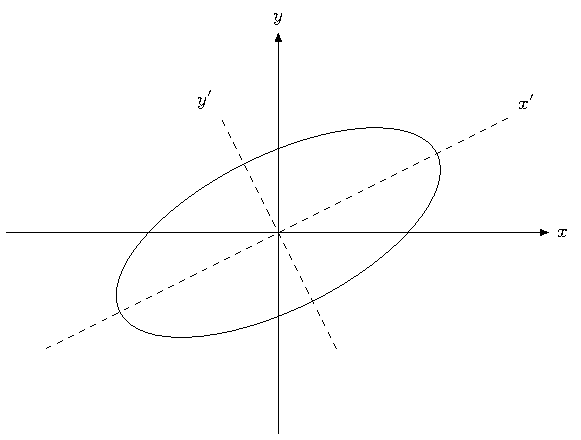
\includegraphics[width=0.55\textwidth]{figuras/6-5-elipse-ejes-rotados.pdf}
    \end{figure}

    Notemos que la matriz $P$ anterior tiene la forma
    \begin{equation*}
        \begin{pmatrix}\cos\theta&-\sin\theta\\\sin\theta&\cos\theta\end{pmatrix},
    \end{equation*}
    donde $\theta=\cos^{-1}\dfrac{2}{\sqrt5}\approx26.6^\circ$. Así, $P$ es la representación matricial de una rotación de $\R^2$ por el ángulo $\theta$. Por tanto, el cambio de variable $X=PX'$ puede lograrse mediante esta rotación de los ejes $x$ e $y$.

    Hay otra posibilidad para $P$: si el vector propio de $A$ correspondiente al valor propio $6$ se toma como $(1,-2)$ en lugar de $(-1,2)$, y se intercambian los valores propios, obtenemos la matriz
    \begin{equation*}
        \begin{pmatrix}\frac{1}{\sqrt5}&\frac{2}{\sqrt5}\\\frac{-2}{\sqrt5}&\frac{1}{\sqrt5}\end{pmatrix},
    \end{equation*}
    que es la representación matricial de una rotación por el ángulo $\theta=\sin^{-1}\!\left(-\dfrac{2}{\sqrt5}\right)\approx-63.4^\circ$. Esta posibilidad produce la misma elipse que la de la figura anterior, pero intercambia los nombres de los ejes $x'$ y $y'$.

    \section{Proyecciones ortogonales y el teorema espectral}

    En esta sección nos apoyamos fuertemente en los teoremas vistos en la Sección~6.4 para desarrollar una representación elegante de un operador normal (si $F=\C$) o autoadjunto (si $F=\R$) $T$ sobre un espacio con producto interno de dimensión finita. Probamos que $T$ puede escribirse en la forma $\lambda_1T_1+\lambda_2T_2+\cdots+\lambda_kT_k$, donde $\lambda_1,\lambda_2,\dots,\lambda_k$ son los valores propios distintos de $T$, y $T_1,T_2,\dots,T_k$ son \textit{proyecciones ortogonales}. Antes debemos desarrollar algunos resultados sobre estas proyecciones especiales.

    Recordemos que, si $V=W_1\oplus W_2$, un operador lineal $T$ sobre $V$ es la \textbf{proyección sobre $W_1$ a lo largo de $W_2$} si, para cada $x=x_1+x_2$ con $x_1\in W_1$ y $x_2\in W_2$, se tiene $T(x)=x_1$. En este caso,
    \begin{equation*}
        \Im(T)=W_1=\{x\in V:T(x)=x\} \qquad\text{y}\qquad \ker(T)=W_2.
    \end{equation*}
    En efecto, si $x\in W_1$, entonces $x=x+0$ es la descomposición de $x$ con la primera componente en $W_1$ y la segunda en $W_2$, así que $T(x)=x$; recíprocamente, si $T(x)=x$, entonces, escribiendo $x=x_1+x_2$ como arriba, $x_1=T(x)=x$, así que $x_2=0$ y $x\in W_1$. Esto prueba la primera igualdad; además, claramente $\Im(T)\subseteq W_1$ (pues $T(x)=x_1\in W_1$ siempre), lo cual, junto con $W_1\subseteq\Im(T)$ recién probado, da la igualdad. Para la segunda, $T(x)=0$ si y solo si $x_1=0$, si y solo si $x=x_2\in W_2$.

    Así, $V=\Im(T)\oplus\ker(T)$, y no hay ambigüedad si nos referimos a $T$ como la \textquotedblleft proyección sobre $W_1$\textquotedblright, o simplemente como una \textquotedblleft proyección\textquotedblright. De hecho, $T$ es una proyección si y solo si $T=T^2$: si $T$ es la proyección sobre $W_1$ a lo largo de $W_2$, entonces, para $x=x_1+x_2$, $T^2(x)=T(x_1)=x_1=T(x)$ (pues $x_1\in W_1$ se descompone trivialmente como $x_1+0$), así que $T^2=T$. Recíprocamente, supongamos que $T^2=T$, y sean $W_1=\Im(T)$ y $W_2=\ker(T)$. Para cualquier $x\in V$, $x=T(x)+(x-T(x))$, donde $T(x)\in W_1$ claramente, y $x-T(x)\in W_2$ porque $T(x-T(x))=T(x)-T^2(x)=T(x)-T(x)=0$; así $V=W_1+W_2$. Si $y\in W_1\cap W_2$, entonces $y=T(z)$ para algún $z$, y $T(y)=0$; pero $T(y)=T(T(z))=T^2(z)=T(z)=y$, así que $y=0$; por tanto $V=W_1\oplus W_2$. Finalmente, si $x=x_1+x_2$ con $x_1\in W_1,x_2\in W_2$, entonces $x_1=T(z)$ para algún $z$, así que $T(x_1)=T^2(z)=T(z)=x_1$, y por tanto $T(x)=T(x_1)+T(x_2)=x_1+0=x_1$; así $T$ es la proyección sobre $W_1$ a lo largo de $W_2$.

    Como $V=W_1\oplus W_2=W_1\oplus W_3$ no implica que $W_2=W_3$, vemos que $W_1$ no determina de manera única a $T$. Para una \textit{proyección ortogonal} $T$, sin embargo, $T$ queda determinado de manera única por su imagen.

    \begin{definicion}[Proyección ortogonal]
        Sea $V$ un espacio con producto interno, y sea $T:V\to V$ una proyección. Decimos que $T$ es una \textbf{proyección ortogonal} si $\Im(T)^\perp=\ker(T)$ y $\ker(T)^\perp=\Im(T)$.
    \end{definicion}

    Notemos que, si $V$ es de dimensión finita, basta suponer que se cumple una de las dos condiciones anteriores. En efecto, si $\Im(T)^\perp=\ker(T)$, entonces, tomando complementos ortogonales de ambos lados y usando que $W^{\perp\perp}=W$ para todo subespacio $W$ de un espacio con producto interno de dimensión finita (consecuencia del teorema de la Sección~6.2), obtenemos $\Im(T)=\Im(T)^{\perp\perp}=\ker(T)^\perp$.

    Supongamos ahora que $W$ es un subespacio de dimensión finita de un espacio con producto interno $V$. En la notación del teorema visto en la Sección~6.2, podemos definir una función $T:V\to V$ por $T(y)=u$, donde $y=u+z$ con $u\in W$ y $z\in W^\perp$. Es fácil mostrar que $T$ es la proyección ortogonal de $V$ sobre $W$: claramente $\Im(T)=W$ y $\ker(T)=W^\perp$ (pues $T(y)=0$ si y solo si $u=0$, si y solo si $y=z\in W^\perp$), y $W^\perp=\ker(T)$, $W^{\perp\perp}=\Im(T)$ son precisamente las condiciones requeridas. Podemos decir aún más: existe exactamente una proyección ortogonal sobre $W$. Pues, si $T$ y $U$ son proyecciones ortogonales sobre $W$, entonces $\Im(T)=W=\Im(U)$. Así, $\ker(T)=\Im(T)^\perp=\Im(U)^\perp=\ker(U)$, y como toda proyección queda determinada de manera única por su imagen y su núcleo, tenemos $T=U$. Llamamos a $T$ la \textbf{proyección ortogonal} de $V$ sobre $W$.

    Para entender la diferencia geométrica entre una proyección arbitraria sobre $W$ y la proyección ortogonal sobre $W$, sean $V=\R^2$ y $W=\gen{\{(1,1)\}}$. Definamos $U$ y $T$ como en la siguiente figura, donde $T(v)$ es el pie de una perpendicular trazada desde $v$ a la recta $y=x$, y $U(a_1,a_2)=(a_1,a_1)$. Entonces $T$ es la proyección ortogonal de $V$ sobre $W$, y $U$ es otra proyección sobre $W$. Notemos que $v-T(v)\in W^\perp$, mientras que $v-U(v)\notin W^\perp$.

    \begin{figure}[H]
        \centering
        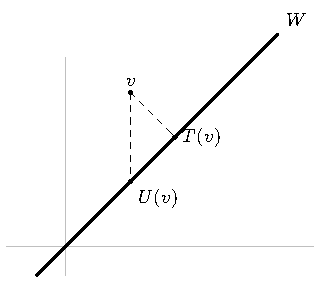
\includegraphics[width=0.55\textwidth]{figuras/6-6-proyeccion-ortogonal-vs-oblicua.pdf}
    \end{figure}

    De la figura anterior vemos que $T(v)$ es la \textquotedblleft mejor aproximación en $W$ a $v$\textquotedblright; es decir, si $w\in W$, entonces $\norm{w-v}\geq\norm{T(v)-v}$. De hecho, esta propiedad de aproximación caracteriza a $T$. Estos resultados se siguen de inmediato del corolario al teorema visto en la Sección~6.2.

    Como aplicación al análisis de Fourier, recordemos el espacio con producto interno $H$ y el conjunto ortonormal $S$ de un ejemplo de la Sección~6.1. Definamos un \textbf{polinomio trigonométrico de grado} $n$ como una función $g\in H$ de la forma
    \begin{equation*}
        g(t)=\sum_{j=-n}^{n}a_jf_j(t)=\sum_{j=-n}^{n}a_je^{ijt},
    \end{equation*}
    donde $a_n$ o $a_{-n}$ es no nulo.

    Sea $f\in H$. Mostramos que la mejor aproximación a $f$ mediante un polinomio trigonométrico de grado menor o igual a $n$ es el polinomio trigonométrico cuyos coeficientes son los coeficientes de Fourier de $f$ relativos al conjunto ortonormal $S$. Para este resultado, sea $W=\gen{\{f_j:|j|\leq n\}}$, y sea $T$ la proyección ortogonal de $H$ sobre $W$. El corolario al teorema visto en la Sección~6.2 nos dice que la mejor aproximación a $f$ mediante una función en $W$ es
    \begin{equation*}
        T(f)=\sum_{j=-n}^{n}\iprod{f}{f_j}f_j.
    \end{equation*}

    A continuación damos una caracterización algebraica de las proyecciones ortogonales.

    \begin{teorema}
        Sea $V$ un espacio con producto interno, y sea $T$ un operador lineal sobre $V$. Entonces $T$ es una proyección ortogonal si y solo si $T$ tiene adjunto $T^*$ y $T^2=T=T^*$.
    \end{teorema}

    \begin{proof}
        Supongamos que $T$ es una proyección ortogonal. Como $T^2=T$ por ser $T$ una proyección, basta mostrar que $T^*$ existe y que $T=T^*$. Ahora $V=\Im(T)\oplus\ker(T)$, con $\Im(T)^\perp=\ker(T)$. Sean $x,y\in V$. Podemos escribir $x=x_1+x_2$ y $y=y_1+y_2$, donde $x_1,y_1\in\Im(T)$ y $x_2,y_2\in\ker(T)$. Así
        \begin{equation*}
            \iprod{x}{T(y)}=\iprod{x_1+x_2}{y_1}=\iprod{x_1}{y_1}+\iprod{x_2}{y_1}=\iprod{x_1}{y_1}
        \end{equation*}
        y
        \begin{equation*}
            \iprod{T(x)}{y}=\iprod{x_1}{y_1+y_2}=\iprod{x_1}{y_1}+\iprod{x_1}{y_2}=\iprod{x_1}{y_1}.
        \end{equation*}
        Así $\iprod{T(x)}{y}=\iprod{x}{T(y)}$ para todos $x,y\in V$; por tanto $T^*$ existe y $T=T^*$.

        Recíprocamente, supongamos que $T^2=T=T^*$. Entonces $T$ es una proyección, por lo que solo falta mostrar que $\Im(T)^\perp=\ker(T)$ y $\ker(T)^\perp=\Im(T)$. Sean $x\in\Im(T)$ y $y\in\ker(T)$. Entonces $x=T(x)=T^*(x)$, así que
        \begin{equation*}
            \iprod{x}{y}=\iprod{T^*(x)}{y}=\iprod{x}{T(y)}=\iprod{x}{0}=0.
        \end{equation*}
        Por tanto $x\in\ker(T)^\perp$, de donde se sigue que $\Im(T)\subseteq\ker(T)^\perp$.

        Ahora mostremos que $y\in\Im(T)$, es decir, que $T(y)=y$. Sea $y\in\ker(T)^\perp$. Ahora
        \begin{align*}
            \norm{y-T(y)}^2&=\iprod{y-T(y)}{y-T(y)}\\
            &=\iprod{y}{y-T(y)}-\iprod{T(y)}{y-T(y)}.
        \end{align*}
        Como $y-T(y)\in\ker(T)$ (pues $T(y-T(y))=T(y)-T^2(y)=0$), el primer término debe ser cero, ya que $y\in\ker(T)^\perp$. Pero también
        \begin{equation*}
            \iprod{T(y)}{y-T(y)}=\iprod{y}{T^*(y-T(y))}=\iprod{y}{T(y-T(y))}=\iprod{y}{0}=0.
        \end{equation*}
        Así $\norm{y-T(y)}^2=0$; es decir, $y-T(y)=0$, así que $y=T(y)\in\Im(T)$. Por tanto $\ker(T)^\perp\subseteq\Im(T)$.

        Combinando ambas inclusiones probadas, $\Im(T)\subseteq\ker(T)^\perp$ y $\ker(T)^\perp\subseteq\Im(T)$, obtenemos $\ker(T)^\perp=\Im(T)$. Usando $W^{\perp\perp}=W$ (válido para subespacios de dimensión finita, o directamente verificable aquí), se sigue también que $\Im(T)^\perp=\ker(T)^{\perp\perp}=\ker(T)$.
    \end{proof}

    Sea $V$ un espacio con producto interno de dimensión finita, $W$ un subespacio de $V$, y $T$ la proyección ortogonal de $V$ sobre $W$. Podemos elegir una base ortonormal $\BB=\{v_1,v_2,\dots,v_n\}$ para $V$ tal que $\{v_1,v_2,\dots,v_k\}$ sea una base de $W$. Entonces $[T]_{\BB}$ es una matriz diagonal con unos en las primeras $k$ entradas diagonales y ceros en el resto. De hecho, $[T]_{\BB}$ tiene la forma
    \begin{equation*}
        \begin{pmatrix}I_k&O_1\\O_2&O_3\end{pmatrix}.
    \end{equation*}
    Si $U$ es cualquier proyección sobre $W$, podemos elegir una base $\gamma$ de $V$ tal que $[U]_\gamma$ tenga la forma anterior; sin embargo, $\gamma$ no es necesariamente ortonormal.

    Estamos ya listos para el teorema principal de esta sección.

    \begin{teorema}[Teorema espectral]
        Supongamos que $T$ es un operador lineal sobre un espacio con producto interno de dimensión finita $V$ sobre $F$, con valores propios distintos $\lambda_1,\lambda_2,\dots,\lambda_k$. Supongamos que $T$ es normal si $F=\C$ y que $T$ es autoadjunto si $F=\R$. Para cada $i$ ($1\leq i\leq k$), sea $W_i$ el subespacio propio de $T$ correspondiente al valor propio $\lambda_i$, y sea $T_i$ la proyección ortogonal de $V$ sobre $W_i$. Entonces se cumple lo siguiente:
        \begin{enumerate}[label=(\alph*)]
            \item $V=W_1\oplus W_2\oplus\cdots\oplus W_k$.
            \item Si $W_i'$ denota la suma directa de los subespacios $W_j$ con $j\neq i$, entonces $W_i^\perp=W_i'$.
            \item $T_iT_j=\delta_{ij}T_i$ para $1\leq i,j\leq k$.
            \item $I=T_1+T_2+\cdots+T_k$.
            \item $T=\lambda_1T_1+\lambda_2T_2+\cdots+\lambda_kT_k$.
        \end{enumerate}
    \end{teorema}

    \begin{proof}
        (a) Por los teoremas vistos en la Sección~6.4, $T$ es diagonalizable, así que
        \begin{equation*}
            V=W_1\oplus W_2\oplus\cdots\oplus W_k
        \end{equation*}
        por el teorema visto en el Capítulo~1 sobre operadores diagonalizables y sumas directas de subespacios propios.

        (b) Si $x\in W_i$ y $y\in W_j$ para algún $i\neq j$, entonces $\iprod{x}{y}=0$ por el teorema visto en la Sección~6.4 sobre operadores normales (ortogonalidad de vectores propios correspondientes a valores propios distintos). Se sigue fácilmente de este hecho que $W_i'\subseteq W_i^\perp$. De (a), tenemos
        \begin{equation*}
            \dim(W_i')=\sum_{j\neq i}\dim(W_j)=\dim(V)-\dim(W_i).
        \end{equation*}
        Por otro lado, tenemos $\dim(W_i^\perp)=\dim(V)-\dim(W_i)$ por el teorema visto en la Sección~6.2. Por tanto $W_i'=W_i^\perp$, lo cual prueba (b).

        (c) Como $T_i$ es la proyección ortogonal sobre $W_i$, sabemos que $T_i^2=T_i$. Sea $j\neq i$. Por (b), $\ker(T_i)=W_i^\perp=W_i'\supseteq W_j$; así, para $x\in V$, $T_j(x)\in W_j\subseteq\ker(T_i)$, de donde $T_i(T_j(x))=0$. Por tanto $T_iT_j=T_0=\delta_{ij}T_i$ para $i\neq j$, y $T_iT_i=T_i^2=T_i=\delta_{ii}T_i$; así $T_iT_j=\delta_{ij}T_i$ en todos los casos.

        (d) Como $T_i$ es la proyección ortogonal sobre $W_i$, se sigue de (b) que $\ker(T_i)=W_i^\perp=W_i'$. De (a), para $x\in V$, $x=x_1+x_2+\cdots+x_k$, donde $x_i\in W_i$ para cada $i$. Entonces
        \begin{equation*}
            I(x)=x=x_1+x_2+\cdots+x_k=T_1(x)+T_2(x)+\cdots+T_k(x)=(T_1+T_2+\cdots+T_k)(x),
        \end{equation*}
        pues $T_i(x)=x_i$ (ya que $x_i\in W_i$ y los demás sumandos están en $\ker(T_i)=W_i'$). Así $I=T_1+T_2+\cdots+T_k$, probando (d).

        (e) Para $x\in V$, escribamos $x=x_1+x_2+\cdots+x_k$, donde $x_i\in W_i$. Entonces
        \begin{align*}
            T(x)&=T(x_1)+T(x_2)+\cdots+T(x_k)\\
            &=\lambda_1x_1+\lambda_2x_2+\cdots+\lambda_kx_k\\
            &=\lambda_1T_1(x)+\lambda_2T_2(x)+\cdots+\lambda_kT_k(x)\\
            &=(\lambda_1T_1+\lambda_2T_2+\cdots+\lambda_kT_k)(x).
        \end{align*}
    \end{proof}

    Al conjunto $\{\lambda_1,\lambda_2,\dots,\lambda_k\}$ de valores propios de $T$ se le llama el \textbf{espectro} de $T$; a la suma $I=T_1+T_2+\cdots+T_k$ de (d) se le llama la \textbf{resolución de la identidad} inducida por $T$; y a la suma $T=\lambda_1T_1+\lambda_2T_2+\cdots+\lambda_kT_k$ de (e) se le llama la \textbf{descomposición espectral} de $T$. La descomposición espectral de $T$ es única salvo por el orden de sus valores propios.

    Con la notación anterior, sea $\BB$ la unión de bases ortonormales de los $W_i$, y sea $m_i=\dim(W_i)$ (así, $m_i$ es la multiplicidad de $\lambda_i$). Entonces $[T]_{\BB}$ tiene la forma
    \begin{equation*}
        \begin{pmatrix}\lambda_1I_{m_1}&O&\cdots&O\\O&\lambda_2I_{m_2}&\cdots&O\\\vdots&&&\vdots\\O&O&\cdots&\lambda_kI_{m_k}\end{pmatrix};
    \end{equation*}
    es decir, $[T]_{\BB}$ es una matriz diagonal cuyas entradas diagonales son los valores propios $\lambda_i$ de $T$, y cada $\lambda_i$ se repite $m_i$ veces. Si $\lambda_1T_1+\lambda_2T_2+\cdots+\lambda_kT_k$ es la descomposición espectral de $T$, entonces se sigue (aplicando ambos lados a cada vector de una base $\BB$ como la anterior, y usando que $g(T_i(v))=g(\lambda_i)v$ para $v\in W_i$, junto con (c)) que $g(T)=g(\lambda_1)T_1+g(\lambda_2)T_2+\cdots+g(\lambda_k)T_k$ para cualquier polinomio $g$. Este hecho se usa a continuación.

    Enumeramos ahora varios corolarios interesantes del teorema espectral. En lo que sigue, suponemos que $T$ es un operador lineal sobre un espacio con producto interno de dimensión finita $V$ sobre $F$.

    \begin{corolario}
        Si $F=\C$, entonces $T$ es normal si y solo si $T^*=g(T)$ para algún polinomio $g$.
    \end{corolario}

    \begin{proof}
        Supongamos primero que $T$ es normal. Sea $T=\lambda_1T_1+\lambda_2T_2+\cdots+\lambda_kT_k$ la descomposición espectral de $T$. Tomando el adjunto de ambos lados de la ecuación anterior, tenemos $T^*=\overline{\lambda_1}T_1+\overline{\lambda_2}T_2+\cdots+\overline{\lambda_k}T_k$, pues cada $T_i$ es autoadjunto. Usando la fórmula de interpolación de Lagrange (ya vista en el primer curso), podemos elegir un polinomio $g$ tal que $g(\lambda_i)=\overline{\lambda_i}$ para $1\leq i\leq k$. Entonces
        \begin{equation*}
            g(T)=g(\lambda_1)T_1+g(\lambda_2)T_2+\cdots+g(\lambda_k)T_k=\overline{\lambda_1}T_1+\overline{\lambda_2}T_2+\cdots+\overline{\lambda_k}T_k=T^*.
        \end{equation*}

        Recíprocamente, si $T^*=g(T)$ para algún polinomio $g$, entonces $T$ conmuta con $T^*$, pues $T$ conmuta con todo polinomio en $T$. Así $T$ es normal.
    \end{proof}

    \begin{corolario}
        Si $F=\C$, entonces $T$ es unitario si y solo si $T$ es normal y $|\lambda|=1$ para todo valor propio $\lambda$ de $T$.
    \end{corolario}

    \begin{proof}
        Si $T$ es unitario, entonces $T$ es normal y todo valor propio de $T$ tiene valor absoluto $1$, por el corolario visto en la Sección~6.5.

        Sea $T=\lambda_1T_1+\lambda_2T_2+\cdots+\lambda_kT_k$ la descomposición espectral de $T$. Si $|\lambda|=1$ para todo valor propio $\lambda$ de $T$, entonces, por (c) del teorema espectral,
        \begin{align*}
            TT^*&=(\lambda_1T_1+\lambda_2T_2+\cdots+\lambda_kT_k)(\overline{\lambda_1}T_1+\overline{\lambda_2}T_2+\cdots+\overline{\lambda_k}T_k)\\
            &=|\lambda_1|^2T_1+|\lambda_2|^2T_2+\cdots+|\lambda_k|^2T_k\\
            &=T_1+T_2+\cdots+T_k\\
            &=I.
        \end{align*}
        Por tanto $T$ es unitario.
    \end{proof}

    \begin{corolario}
        Si $F=\C$ y $T$ es normal, entonces $T$ es autoadjunto si y solo si todo valor propio de $T$ es real.
    \end{corolario}

    \begin{proof}
        Sea $T=\lambda_1T_1+\lambda_2T_2+\cdots+\lambda_kT_k$ la descomposición espectral de $T$. Supongamos que todo valor propio de $T$ es real. Entonces
        \begin{equation*}
            T^*=\overline{\lambda_1}T_1+\overline{\lambda_2}T_2+\cdots+\overline{\lambda_k}T_k=\lambda_1T_1+\lambda_2T_2+\cdots+\lambda_kT_k=T.
        \end{equation*}

        El recíproco ya fue probado en el lema visto en la Sección~6.4.
    \end{proof}

    \begin{corolario}
        Sea $T$ como en el teorema espectral, con descomposición espectral $T=\lambda_1T_1+\lambda_2T_2+\cdots+\lambda_kT_k$. Entonces cada $T_j$ es un polinomio en $T$.
    \end{corolario}

    \begin{proof}
        Elijamos un polinomio $g_j$ ($1\leq j\leq k$) tal que $g_j(\lambda_i)=\delta_{ij}$ para $1\leq i\leq k$. Entonces
        \begin{equation*}
            g_j(T)=g_j(\lambda_1)T_1+g_j(\lambda_2)T_2+\cdots+g_j(\lambda_k)T_k=\delta_{1j}T_1+\delta_{2j}T_2+\cdots+\delta_{kj}T_k=T_j.
        \end{equation*}
    \end{proof}

    \section{La descomposición en valores singulares y la pseudoinversa}

    En la Sección~6.4 caracterizamos a los operadores normales sobre espacios complejos y a los operadores autoadjuntos sobre espacios reales en términos de bases ortonormales de vectores propios y sus valores propios correspondientes. En esta sección establecemos un teorema comparable cuyo alcance abarca a toda la clase de transformaciones lineales entre espacios con producto interno de dimensión finita, tanto complejos como reales: el \textit{teorema de los valores singulares} para transformaciones lineales. Hay similitudes y diferencias entre estos teoremas. Todos se apoyan en el uso de bases ortonormales e invariantes numéricos. Sin embargo, debido a su alcance más general, el teorema de los valores singulares involucra dos espacios con producto interno (usualmente distintos) y dos bases ortonormales (usualmente distintas). Si los dos espacios y las dos bases fueran idénticos, la transformación sería, de hecho, un operador normal o autoadjunto. Otra diferencia es que los invariantes numéricos en el teorema de los valores singulares, los \textit{valores singulares}, son no negativos, a diferencia de sus contrapartes, los valores propios, para los cuales no existe tal restricción. Esta propiedad es necesaria para garantizar la unicidad de los valores singulares.

    El teorema de los valores singulares abarca tanto espacios reales como complejos. Por brevedad, en esta sección usamos los términos \textit{operador unitario} y \textit{matriz unitaria} para incluir también a los operadores ortogonales y a las matrices ortogonales del caso real. Así, cualquier operador $T$ tal que $\iprod{T(x)}{T(y)}=\iprod{x}{y}$, o cualquier matriz $A$ tal que $\iprod{Ax}{Ay}=\iprod{x}{y}$, para todos $x,y$, se llama unitario para los propósitos de esta sección.

    Extendemos primero la definición del adjunto de un operador a cualquier transformación lineal entre espacios con producto interno de dimensión finita. Sean $V$ y $W$ espacios con producto interno de dimensión finita, y sea $T:V\to W$ una transformación lineal. Fijemos bases ortonormales $\beta$ de $V$ y $\gamma$ de $W$, y sea $A=[T]_\gamma^\beta$. Definimos $T^*:W\to V$ como la única transformación lineal tal que $[T^*]_\beta^\gamma=A^*$; se verifica, exactamente como en la Sección~6.3 (usando las bases ortonormales $\beta$ y $\gamma$ en lugar de una sola base), que $T^*$ así definida es la única transformación lineal de $W$ a $V$ que satisface
    \begin{equation*}
        \iprod{T(x)}{y}_W=\iprod{x}{T^*(y)}_V \qquad \text{para todos } x\in V,\ y\in W,
    \end{equation*}
    y que esta propiedad caracteriza a $T^*$ independientemente de la elección de $\beta$ y $\gamma$. A $T^*$ se le sigue llamando el \textbf{adjunto} de $T$.

    Con esto, el operador $T^*T$ sobre $V$ es \textbf{positivo semidefinido}: es autoadjunto, pues $(T^*T)^*=T^*T^{**}=T^*T$, y $\iprod{T^*T(x)}{x}=\iprod{T(x)}{T(x)}=\norm{T(x)}^2\geq0$ para todo $x\in V$. (En general, decimos que un operador autoadjunto $U$ sobre un espacio con producto interno es \textbf{positivo semidefinido} si $\iprod{U(x)}{x}\geq0$ para todo $x$, y \textbf{positivo definido} si, además, $\iprod{U(x)}{x}>0$ para todo $x\neq0$.) Además, $\rg(T^*T)=\rg(T)$: si $x\in\ker(T)$, entonces claramente $T^*T(x)=T^*(0)=0$; recíprocamente, si $T^*T(x)=0$, entonces $0=\iprod{T^*T(x)}{x}=\iprod{T(x)}{T(x)}$, así que $T(x)=0$. Por tanto $\ker(T^*T)=\ker(T)$, y el resultado se sigue del teorema de la dimensión.

    Con estos hechos en mente, comenzamos con el resultado principal.

    \begin{teorema}[Teorema de los valores singulares para transformaciones lineales]
        Sean $V$ y $W$ espacios con producto interno de dimensión finita, y sea $T:V\to W$ una transformación lineal de rango $r$. Entonces existen bases ortonormales $\{v_1,v_2,\dots,v_n\}$ de $V$ y $\{u_1,u_2,\dots,u_m\}$ de $W$, y escalares positivos $\sigma_1\geq\sigma_2\geq\cdots\geq\sigma_r$, tales que
        \begin{equation*}
            T(v_i)=\begin{cases}\sigma_iu_i&\text{si }1\leq i\leq r\\0&\text{si }i>r.\end{cases}
        \end{equation*}
        Recíprocamente, si se satisfacen las condiciones anteriores, entonces, para $1\leq i\leq n$, $v_i$ es un vector propio de $T^*T$ con valor propio correspondiente $\sigma_i^2$ si $1\leq i\leq r$, y $0$ si $i>r$. Por lo tanto, los escalares $\sigma_1,\sigma_2,\dots,\sigma_r$ están determinados de manera única por $T$.
    \end{teorema}

    \begin{proof}
        Establecemos primero la existencia de las bases y los escalares. Como $T^*T$ es un operador lineal positivo semidefinido de rango $r$ sobre $V$, es en particular autoadjunto; así, existe una base ortonormal $\{v_1,v_2,\dots,v_n\}$ de $V$ formada por vectores propios de $T^*T$, con valores propios correspondientes $\lambda_1\geq\lambda_2\geq\cdots\geq\lambda_n\geq0$. Como $\rg(T^*T)=r$, exactamente $r$ de estos valores propios son no nulos; reordenando si es necesario, podemos suponer que $\lambda_i>0$ para $1\leq i\leq r$ y $\lambda_i=0$ para $i>r$ (los valores propios son no negativos porque, para un vector propio $v_i$ con valor propio $\lambda_i$, $0\leq\norm{T(v_i)}^2=\iprod{T^*T(v_i)}{v_i}=\lambda_i\norm{v_i}^2$).

        Para $1\leq i\leq r$, definamos $\sigma_i=\sqrt{\lambda_i}$ y $u_i=\dfrac{1}{\sigma_i}T(v_i)$. Mostramos que $\{u_1,u_2,\dots,u_r\}$ es un subconjunto ortonormal de $W$. Supongamos $1\leq i,j\leq r$. Entonces
        \begin{align*}
            \iprod{u_i}{u_j}=\iprod{\frac{1}{\sigma_i}T(v_i)}{\frac{1}{\sigma_j}T(v_j)}=\frac{1}{\sigma_i\sigma_j}\iprod{T^*T(v_i)}{v_j}=\frac{1}{\sigma_i\sigma_j}\iprod{\lambda_iv_i}{v_j}=\frac{\sigma_i^2}{\sigma_i\sigma_j}\iprod{v_i}{v_j}=\delta_{ij},
        \end{align*}
        y por tanto $\{u_1,u_2,\dots,u_r\}$ es ortonormal. Por el teorema visto en la Sección~6.2, este conjunto se extiende a una base ortonormal $\{u_1,u_2,\dots,u_r,\dots,u_m\}$ de $W$. Claramente $T(v_i)=\sigma_iu_i$ si $1\leq i\leq r$. Si $i>r$, entonces $\lambda_i=0$, así que $T^*T(v_i)=0$; luego $0=\iprod{T^*T(v_i)}{v_i}=\iprod{T(v_i)}{T(v_i)}$, y por tanto $T(v_i)=0$.

        Para probar la unicidad, supongamos que $\{v_1,v_2,\dots,v_n\}$, $\{u_1,u_2,\dots,u_m\}$ y $\sigma_1\geq\sigma_2\geq\cdots\geq\sigma_r>0$ satisfacen las condiciones enunciadas en la primera parte del teorema. Para $1\leq i\leq m$ y $1\leq j\leq n$,
        \begin{equation*}
            \iprod{T^*(u_i)}{v_j}=\iprod{u_i}{T(v_j)}=\begin{cases}\sigma_i&\text{si }i=j\leq r\\0&\text{en otro caso,}\end{cases}
        \end{equation*}
        y por tanto, para cualquier $1\leq i\leq m$,
        \begin{equation*}
            T^*(u_i)=\sum_{j=1}^{n}\iprod{T^*(u_i)}{v_j}v_j=\begin{cases}\sigma_iv_i&\text{si }i=j\leq r\\0&\text{en otro caso.}\end{cases}
        \end{equation*}
        Así, para $i\leq r$,
        \begin{equation*}
            T^*T(v_i)=T^*(\sigma_iu_i)=\sigma_iT^*(u_i)=\sigma_i^2v_i,
        \end{equation*}
        y $T^*T(v_i)=T^*(0)=0$ para $i>r$. Por tanto, cada $v_i$ es un vector propio de $T^*T$ con valor propio correspondiente $\sigma_i^2$ si $i\leq r$, y $0$ si $i>r$.
    \end{proof}

    \begin{definicion}[Valores singulares]
        Los escalares únicos $\sigma_1,\sigma_2,\dots,\sigma_r$ del teorema anterior se llaman los \textbf{valores singulares} de $T$. Si $r$ es menor tanto que $m$ como que $n$, el término valor singular se extiende para incluir $\sigma_{r+1}=\cdots=\sigma_k=0$, donde $k$ es el mínimo entre $m$ y $n$.
    \end{definicion}

    Aunque los valores singulares de una transformación lineal $T$ están determinados de manera única por $T$, las bases ortonormales dadas en el enunciado del teorema anterior no lo están, pues existe más de una base ortonormal de vectores propios de $T^*T$.

    Por lo visto en la demostración anterior, los valores singulares de una transformación lineal $T:V\to W$ y de su adjunto $T^*$ son idénticos. Más aún, las bases ortonormales de $V$ y $W$ dadas en el teorema anterior simplemente se intercambian para $T^*$.

    \begin{ejemplo}
        Sean $P_2(\R)$ y $P_1(\R)$ los espacios de polinomios con producto interno definido por
        \begin{equation*}
            \iprod{f(x)}{g(x)}=\int_{-1}^{1}f(t)g(t)\,dt.
        \end{equation*}
        Sea $T:P_2(\R)\to P_1(\R)$ la transformación lineal definida por $T(f(x))=f'(x)$. Encontramos bases ortonormales $\beta=\{v_1,v_2,v_3\}$ de $P_2(\R)$ y $\gamma=\{u_1,u_2\}$ de $P_1(\R)$ tales que $T(v_i)=\sigma_iu_i$ para $i=1,2$ y $T(v_3)=0$, donde $\sigma_1\geq\sigma_2>0$ son los valores singulares no nulos de $T$.

        Para facilitar los cálculos, traducimos este problema al problema correspondiente para una representación matricial de $T$. Debemos usar una representación matricial construida a partir de bases ortonormales de $P_2(\R)$ y $P_1(\R)$, para garantizar que el adjunto de la representación matricial de $T$ sea la representación matricial del adjunto de $T$. Para este propósito, usamos las bases ortonormales
        \begin{equation*}
            \alpha=\left\{\frac{1}{\sqrt2},\ \sqrt{\frac32}\,x,\ \sqrt{\frac58}\,(3x^2-1)\right\} \qquad\text{y}\qquad \alpha'=\left\{\frac{1}{\sqrt2},\ \sqrt{\frac32}\,x\right\}
        \end{equation*}
        para $P_2(\R)$ y $P_1(\R)$, respectivamente, obtenidas en la Sección~6.2.

        Sea
        \begin{equation*}
            A=[T]_{\alpha'}^\alpha=\begin{pmatrix}0&\sqrt3&0\\0&0&\sqrt{15}\end{pmatrix}.
        \end{equation*}
        Entonces
        \begin{equation*}
            A^*A=\begin{pmatrix}0&0\\\sqrt3&0\\0&\sqrt{15}\end{pmatrix}\begin{pmatrix}0&\sqrt3&0\\0&0&\sqrt{15}\end{pmatrix}=\begin{pmatrix}0&0&0\\0&3&0\\0&0&15\end{pmatrix},
        \end{equation*}
        cuyos valores propios (en orden decreciente de tamaño) son $\lambda_1=15$, $\lambda_2=3$ y $\lambda_3=0$. Estos valores propios corresponden, respectivamente, a los vectores propios ortonormales $e_3=(0,0,1)$, $e_2=(0,1,0)$ y $e_1=(1,0,0)$ en $\R^3$. Trasladando todo al contexto de $T$, $P_2(\R)$ y $P_1(\R)$, sea
        \begin{equation*}
            v_1=\sqrt{\frac58}\,(3x^2-1), \qquad v_2=\sqrt{\frac32}\,x, \qquad\text{y}\qquad v_3=\frac{1}{\sqrt2}.
        \end{equation*}
        Entonces $\beta=\{v_1,v_2,v_3\}$ es una base ortonormal de $P_2(\R)$ formada por vectores propios de $T^*T$ con valores propios correspondientes $\lambda_1$, $\lambda_2$ y $\lambda_3$. Ahora hacemos $\sigma_1=\sqrt{\lambda_1}=\sqrt{15}$ y $\sigma_2=\sqrt{\lambda_2}=\sqrt3$, los valores singulares no nulos de $T$, y tomamos
        \begin{equation*}
            u_1=\frac{1}{\sigma_1}T(v_1)=\sqrt{\frac32}\,x \qquad\text{y}\qquad u_2=\frac{1}{\sigma_2}T(v_2)=\frac{1}{\sqrt2},
        \end{equation*}
        para obtener la base requerida $\gamma=\{u_1,u_2\}$ de $P_1(\R)$.
    \end{ejemplo}

    Podemos usar los valores singulares para describir cómo una transformación lineal distorsiona una figura. Esto se ilustra en el siguiente ejemplo.

    \begin{ejemplo}
        Sea $T$ un operador lineal invertible sobre $\R^2$, y sea $S=\{x\in\R^2:\norm{x}=1\}$, el círculo unitario en $\R^2$. Aplicamos el teorema anterior para describir $S'=T(S)$.

        Como $T$ es invertible, tiene rango $2$ y, por tanto, valores singulares $\sigma_1\geq\sigma_2>0$. Sean $\{v_1,v_2\}$ y $\BB=\{u_1,u_2\}$ bases ortonormales de $\R^2$ tales que $T(v_1)=\sigma_1u_1$ y $T(v_2)=\sigma_2u_2$, como en el teorema anterior. Entonces $\BB$ determina un sistema de coordenadas $x'y'$ para $\R^2$, donde el eje $x'$ contiene a $u_1$ y el eje $y'$ contiene a $u_2$. Para cualquier vector $u\in\R^2$, si $u=x_1'u_1+x_2'u_2$, entonces $[u]_{\BB}=\left(\begin{smallmatrix}x_1'\\x_2'\end{smallmatrix}\right)$ es el vector de coordenadas de $u$ relativo a $\BB$. Caracterizamos $S'$ en términos de una ecuación que relaciona $x_1'$ y $x_2'$.

        Para cualquier vector $v=x_1v_1+x_2v_2\in\R^2$, la ecuación $u=T(v)$ significa que
        \begin{equation*}
            u=T(x_1v_1+x_2v_2)=x_1T(v_1)+x_2T(v_2)=x_1\sigma_1u_1+x_2\sigma_2u_2.
        \end{equation*}
        Así, para $u=x_1'u_1+x_2'u_2$, tenemos $x_1'=x_1\sigma_1$ y $x_2'=x_2\sigma_2$. Más aún, $u\in S'$ si y solo si $v\in S$ si y solo si
        \begin{equation*}
            \frac{(x_1')^2}{\sigma_1^2}+\frac{(x_2')^2}{\sigma_2^2}=x_1^2+x_2^2=1.
        \end{equation*}
        Si $\sigma_1=\sigma_2$, esta es la ecuación de un círculo de radio $\sigma_1$; y si $\sigma_1>\sigma_2$, es la ecuación de una elipse con semieje mayor y semieje menor orientados a lo largo del eje $x'$ y del eje $y'$, respectivamente. (Véase la siguiente figura.)
    \end{ejemplo}

    \begin{figure}[H]
        \centering
        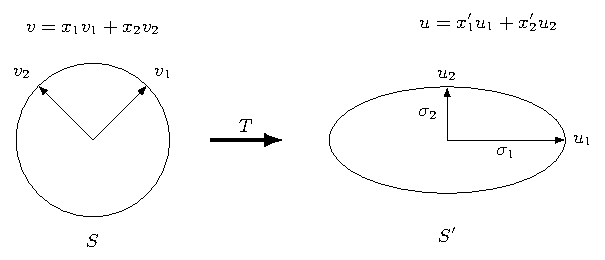
\includegraphics[width=0.85\textwidth]{figuras/6-7-circulo-elipse-valores-singulares.pdf}
    \end{figure}

    El teorema de los valores singulares para transformaciones lineales es útil en su versión matricial, porque podemos realizar cálculos numéricos sobre matrices. Comenzamos con la definición de los valores singulares de una matriz.

    \begin{definicion}[Valores singulares de una matriz]
        Sea $A$ una matriz $m\times n$. Se definen los \textbf{valores singulares} de $A$ como los valores singulares de la transformación lineal $L_A$.
    \end{definicion}

    \begin{teorema}[Teorema de la descomposición en valores singulares para matrices]
        Sea $A$ una matriz $m\times n$ de rango $r$ con valores singulares positivos $\sigma_1\geq\sigma_2\geq\cdots\geq\sigma_r$, y sea $\Sigma$ la matriz $m\times n$ definida por
        \begin{equation*}
            \Sigma_{ij}=\begin{cases}\sigma_i&\text{si }i=j\leq r\\0&\text{en otro caso.}\end{cases}
        \end{equation*}
        Entonces existen una matriz unitaria $U$ de tamaño $m\times m$ y una matriz unitaria $V$ de tamaño $n\times n$ tales que
        \begin{equation*}
            A=U\Sigma V^*.
        \end{equation*}
    \end{teorema}

    \begin{proof}
        Sea $T=L_A:F^n\to F^m$. Por el teorema anterior, existen bases ortonormales $\{v_1,v_2,\dots,v_n\}$ de $F^n$ y $\{u_1,u_2,\dots,u_m\}$ de $F^m$ tales que $T(v_i)=\sigma_iu_i$ para $1\leq i\leq r$ y $T(v_i)=0$ para $i>r$. Sea $U$ la matriz $m\times m$ cuya columna $j$ es $u_j$ para todo $j$, y sea $V$ la matriz $n\times n$ cuya columna $j$ es $v_j$ para todo $j$. Notemos que $U$ y $V$ son matrices unitarias.

        Usando un resultado visto en el primer curso, la columna $j$ de $AV$ es $Av_j=T(v_j)$, la cual es $\sigma_ju_j$ si $j\leq r$, y $0$ si $j>r$. Observemos que la columna $j$ de $\Sigma$ es $\sigma_je_j$, donde $e_j$ es el $j$-ésimo vector canónico de $F^n$ (y $\sigma_j=0$ si $j>r$). Así, la columna $j$ de $U\Sigma$ está dada por
        \begin{equation*}
            U(\sigma_je_j)=\sigma_jU(e_j)=\sigma_ju_j.
        \end{equation*}
        Se sigue que $AV$ y $U\Sigma$ son matrices $m\times n$ cuyas columnas correspondientes son iguales, y por tanto $AV=U\Sigma$. Por lo tanto $A=AVV^*=U\Sigma V^*$.
    \end{proof}

    \begin{definicion}[Descomposición en valores singulares]
        Sea $A$ una matriz $m\times n$ de rango $r$ con valores singulares positivos $\sigma_1\geq\sigma_2\geq\cdots\geq\sigma_r$. Una factorización $A=U\Sigma V^*$, donde $U$ y $V$ son matrices unitarias y $\Sigma$ es la matriz $m\times n$ definida como en el teorema anterior, se llama una \textbf{descomposición en valores singulares} de $A$.
    \end{definicion}

    En la demostración del teorema anterior, las columnas de $V$ son los vectores de la base $\beta$ del primer teorema de esta sección, y las columnas de $U$ son los vectores de la base $\gamma$. Más aún, los valores singulares no nulos de $A$ son los mismos que los de $L_A$; por tanto, son las raíces cuadradas de los valores propios no nulos de $A^*A$ o de $AA^*$.

    \begin{ejemplo}
        Encontramos una descomposición en valores singulares de
        \begin{equation*}
            A=\begin{pmatrix}1&1&-1\\1&1&-1\end{pmatrix}.
        \end{equation*}

        Observemos primero que, para
        \begin{equation*}
            v_1=\frac{1}{\sqrt3}\begin{pmatrix}1\\1\\-1\end{pmatrix}, \qquad v_2=\frac{1}{\sqrt2}\begin{pmatrix}-1\\1\\0\end{pmatrix}, \qquad\text{y}\qquad v_3=\frac{1}{\sqrt6}\begin{pmatrix}1\\1\\2\end{pmatrix},
        \end{equation*}
        el conjunto $\beta=\{v_1,v_2,v_3\}$ es una base ortonormal de $\R^3$ formada por vectores propios de $A^*A$ con valores propios correspondientes $\lambda_1=6$, y $\lambda_2=\lambda_3=0$. En consecuencia, $\sigma_1=\sqrt6$ es el único valor singular no nulo de $A$. Así, como en la demostración del teorema anterior, hacemos que $V$ sea la matriz cuyas columnas son los vectores de $\beta$. Entonces
        \begin{equation*}
            \Sigma=\begin{pmatrix}\sqrt6&0&0\\0&0&0\end{pmatrix} \qquad\text{y}\qquad V=\begin{pmatrix}\frac{1}{\sqrt3}&\frac{-1}{\sqrt2}&\frac{1}{\sqrt6}\\\frac{1}{\sqrt3}&\frac{1}{\sqrt2}&\frac{1}{\sqrt6}\\\frac{-1}{\sqrt3}&0&\frac{2}{\sqrt6}\end{pmatrix}.
        \end{equation*}
        También, como en el teorema anterior, tomamos
        \begin{equation*}
            u_1=\frac{1}{\sigma_1}L_A(v_1)=\frac{1}{\sigma_1}Av_1=\frac{1}{\sqrt2}\begin{pmatrix}1\\1\end{pmatrix}.
        \end{equation*}
        Elegimos ahora $u_2=\dfrac{1}{\sqrt2}\begin{pmatrix}1\\-1\end{pmatrix}$, un vector unitario ortogonal a $u_1$, para obtener la base ortonormal $\gamma=\{u_1,u_2\}$ de $\R^2$, y hacemos
        \begin{equation*}
            U=\begin{pmatrix}\frac{1}{\sqrt2}&\frac{1}{\sqrt2}\\\frac{1}{\sqrt2}&\frac{-1}{\sqrt2}\end{pmatrix}.
        \end{equation*}
        Entonces $A=U\Sigma V^*$ es la descomposición en valores singulares deseada.
    \end{ejemplo}

    \subsection*{La descomposición polar de una matriz cuadrada}

    Una descomposición en valores singulares de una matriz puede usarse para factorizar una matriz cuadrada de manera análoga a la factorización de un número complejo como el producto de un número complejo de longitud $1$ y un número no negativo. En el caso de las matrices, el número complejo de longitud $1$ se reemplaza por una matriz unitaria, y el número no negativo se reemplaza por una matriz positiva semidefinida.

    \begin{teorema}[Descomposición polar]
        Para cualquier matriz cuadrada $A$, existen una matriz unitaria $W$ y una matriz positiva semidefinida $P$ tales que
        \begin{equation*}
            A=WP.
        \end{equation*}
        Más aún, si $A$ es invertible, entonces esta representación es única.
    \end{teorema}

    \begin{proof}
        Por el teorema anterior, existen matrices unitarias $U$ y $V$, y una matriz diagonal $\Sigma$ con entradas no negativas, tales que $A=U\Sigma V^*$. Así
        \begin{equation*}
            A=U\Sigma V^*=UV^*V\Sigma V^*=WP,
        \end{equation*}
        donde $W=UV^*$ y $P=V\Sigma V^*$. Como $W$ es producto de matrices unitarias, $W$ es unitaria. Además, $\Sigma$ es positiva semidefinida, pues, viendo a $\Sigma$ como la matriz de un operador diagonal con entradas diagonales no negativas, $\iprod{\Sigma x}{x}=\sum_i\Sigma_{ii}|x_i|^2\geq0$ para todo $x$; y como $P$ es unitariamente equivalente a $\Sigma$ (vía $V$), $P$ también es positiva semidefinida, pues $\iprod{Px}{x}=\iprod{\Sigma(V^*x)}{V^*x}\geq0$.

        Supongamos ahora que $A$ es invertible, y que $A$ se factoriza también como
        \begin{equation*}
            A=WP=ZQ,
        \end{equation*}
        donde $W$ y $Z$ son unitarias y $P$ y $Q$ son positivas semidefinidas. Como $A$ es invertible, se sigue que $P$ y $Q$ son positivas definidas e invertibles, y por tanto $Z^*W=QP^{-1}$. Así $QP^{-1}$ es unitaria, y por tanto
        \begin{equation*}
            I=(QP^{-1})^*(QP^{-1})=P^{-1}Q^2P^{-1}.
        \end{equation*}
        De aquí, $P^2=Q^2$. Mostramos ahora que $P=Q$. Sea $\lambda$ un valor propio de $P$, con $\lambda>0$ pues $P$ es positiva definida, y sea $E$ el subespacio propio de $P$ correspondiente a $\lambda$. Para $x\in E$, $P^2(x)=\lambda^2x$, y como $P^2=Q^2$, también $Q^2(x)=\lambda^2x$. Por el teorema espectral aplicado a $Q$ (positiva definida, en particular autoadjunta), $Q^2$ tiene la misma descomposición espectral que $Q$ con cada valor propio elevado al cuadrado, y como los valores propios de $Q$ son todos positivos, la función $t\mapsto t^2$ es inyectiva sobre ellos; así, el subespacio propio de $Q^2$ correspondiente al valor propio $\lambda^2$ coincide con el subespacio propio de $Q$ correspondiente al único valor propio positivo $\mu$ de $Q$ tal que $\mu^2=\lambda^2$, es decir, $\mu=\lambda$. Por tanto $x$ es un vector propio de $Q$ con valor propio $\lambda$, para todo $x\in E$. Como esto vale para cada valor propio $\lambda$ de $P$, y $P$ es diagonalizable con $V$ igual a la suma directa de sus subespacios propios, concluimos que $Q$ actúa exactamente como $P$ sobre cada uno de estos subespacios; por tanto $P=Q$. Se sigue que $Z^*W=QP^{-1}=I$, así $W=Z$.
    \end{proof}

    \begin{ejemplo}
        Para encontrar la descomposición polar de
        \begin{equation*}
            A=\begin{pmatrix}11&-5\\-2&10\end{pmatrix},
        \end{equation*}
        comenzamos encontrando una descomposición en valores singulares $U\Sigma V^*$ de $A$. El objetivo es encontrar una base ortonormal $\beta$ de $\R^2$ formada por vectores propios de $A^*A$. Puede mostrarse que
        \begin{equation*}
            v_1=\frac{1}{\sqrt2}\begin{pmatrix}1\\-1\end{pmatrix} \qquad\text{y}\qquad v_2=\frac{1}{\sqrt2}\begin{pmatrix}1\\1\end{pmatrix}
        \end{equation*}
        son vectores propios ortonormales de $A^*A$ con valores propios correspondientes $\lambda_1=200$ y $\lambda_2=50$. Así $\beta=\{v_1,v_2\}$ es una base apropiada. Por tanto $\sigma_1=\sqrt{200}=10\sqrt2$ y $\sigma_2=\sqrt{50}=5\sqrt2$ son los valores singulares de $A$. Tenemos, entonces,
        \begin{equation*}
            V=\begin{pmatrix}\frac{1}{\sqrt2}&\frac{1}{\sqrt2}\\\frac{-1}{\sqrt2}&\frac{1}{\sqrt2}\end{pmatrix} \qquad\text{y}\qquad \Sigma=\begin{pmatrix}10\sqrt2&0\\0&5\sqrt2\end{pmatrix}.
        \end{equation*}
        A continuación encontramos las columnas $u_1$ y $u_2$ de $U$:
        \begin{equation*}
            u_1=\frac{1}{\sigma_1}Av_1=\frac{1}{5}\begin{pmatrix}4\\-3\end{pmatrix} \qquad\text{y}\qquad u_2=\frac{1}{\sigma_2}Av_2=\frac{1}{5}\begin{pmatrix}3\\4\end{pmatrix}.
        \end{equation*}
        Así
        \begin{equation*}
            U=\begin{pmatrix}\frac45&\frac35\\\frac{-3}5&\frac45\end{pmatrix}.
        \end{equation*}
        Por tanto, en la notación del teorema anterior, tenemos
        \begin{equation*}
            W=UV^*=\begin{pmatrix}\frac45&\frac35\\\frac{-3}5&\frac45\end{pmatrix}\begin{pmatrix}\frac{1}{\sqrt2}&\frac{-1}{\sqrt2}\\\frac{1}{\sqrt2}&\frac{1}{\sqrt2}\end{pmatrix}=\frac{1}{5\sqrt2}\begin{pmatrix}7&-1\\1&7\end{pmatrix},
        \end{equation*}
        y
        \begin{equation*}
            P=V\Sigma V^*=\begin{pmatrix}\frac{1}{\sqrt2}&\frac{1}{\sqrt2}\\\frac{-1}{\sqrt2}&\frac{1}{\sqrt2}\end{pmatrix}\begin{pmatrix}10\sqrt2&0\\0&5\sqrt2\end{pmatrix}\begin{pmatrix}\frac{1}{\sqrt2}&\frac{-1}{\sqrt2}\\\frac{1}{\sqrt2}&\frac{1}{\sqrt2}\end{pmatrix}=\frac{5}{\sqrt2}\begin{pmatrix}3&-1\\-1&3\end{pmatrix}.
        \end{equation*}
    \end{ejemplo}

    \subsection*{La pseudoinversa}

    Sean $V$ y $W$ espacios con producto interno de dimensión finita sobre el mismo campo, y sea $T:V\to W$ una transformación lineal. Es deseable contar con una transformación lineal de $W$ a $V$ que capture parte de la esencia de una inversa de $T$, aun cuando $T$ no sea invertible. Un enfoque sencillo para este problema consiste en concentrarse en la \textquotedblleft parte\textquotedblright\ de $T$ que sí es invertible, a saber, la restricción de $T$ a $\ker(T)^\perp$. Sea $L:\ker(T)^\perp\to\Im(T)$ la transformación lineal definida por $L(x)=T(x)$ para todo $x\in\ker(T)^\perp$. Entonces $L$ es invertible, y podemos usar la inversa de $L$ para construir una transformación lineal de $W$ a $V$ que rescate algunos de los beneficios de una inversa de $T$.

    \begin{definicion}[Pseudoinversa]
        Sean $V$ y $W$ espacios con producto interno de dimensión finita sobre el mismo campo, y sea $T:V\to W$ una transformación lineal. Sea $L:\ker(T)^\perp\to\Im(T)$ la transformación lineal definida por $L(x)=T(x)$ para todo $x\in\ker(T)^\perp$. La \textbf{pseudoinversa} (o \textbf{inversa generalizada de Moore–Penrose}) de $T$, denotada $T^\dagger$, se define como la única transformación lineal de $W$ a $V$ tal que
        \begin{equation*}
            T^\dagger(y)=\begin{cases}L^{-1}(y)&\text{si }y\in\Im(T)\\0&\text{si }y\in\Im(T)^\perp.\end{cases}
        \end{equation*}
    \end{definicion}

    La pseudoinversa de una transformación lineal sobre un espacio con producto interno de dimensión finita existe aun si $T$ no es invertible. Más aún, si $T$ es invertible, entonces $T^\dagger=T^{-1}$, pues, en ese caso, $\ker(T)^\perp=V$, y $L$ (según se definió) coincide con $T$.

    Como ejemplo extremo, consideremos la transformación cero $T_0:V\to W$ entre dos espacios con producto interno de dimensión finita $V$ y $W$. Entonces $\Im(T_0)=\{0\}$, y por tanto $T_0^\dagger$ es la transformación cero de $W$ a $V$.

    Podemos usar el teorema de los valores singulares para describir la pseudoinversa de una transformación lineal. Supongamos que $V$ y $W$ son espacios vectoriales de dimensión finita y que $T:V\to W$ es una transformación lineal de rango $r$. Sean $\{v_1,v_2,\dots,v_n\}$ y $\{u_1,u_2,\dots,u_m\}$ bases ortonormales para $V$ y $W$, respectivamente, y sean $\sigma_1\geq\sigma_2\geq\cdots\geq\sigma_r$ los valores singulares no nulos de $T$ que satisfacen la primera parte del teorema de los valores singulares. Entonces $\{v_1,v_2,\dots,v_r\}$ es una base de $\ker(T)^\perp$, $\{v_{r+1},v_{r+2},\dots,v_n\}$ es una base de $\ker(T)$, $\{u_1,u_2,\dots,u_r\}$ es una base de $\Im(T)$, y $\{u_{r+1},u_{r+2},\dots,u_m\}$ es una base de $\Im(T)^\perp$. Sea $L$ la restricción de $T$ a $\ker(T)^\perp$, como en la definición de pseudoinversa. Entonces $L^{-1}(u_i)=\dfrac{1}{\sigma_i}v_i$ para $1\leq i\leq r$. Por tanto,
    \begin{equation*}
        T^\dagger(u_i)=\begin{cases}\dfrac{1}{\sigma_i}v_i&\text{si }1\leq i\leq r\\0&\text{si }r<i\leq m.\end{cases} \tag{6}
    \end{equation*}

    \begin{ejemplo}
        Sea $T:P_2(\R)\to P_1(\R)$ la transformación lineal definida por $T(f(x))=f'(x)$, como en un ejemplo anterior. Sean $\beta=\{v_1,v_2,v_3\}$ y $\gamma=\{u_1,u_2\}$ las bases ortonormales para $P_2(\R)$ y $P_1(\R)$ de dicho ejemplo. Entonces $\sigma_1=\sqrt{15}$ y $\sigma_2=\sqrt3$ son los valores singulares no nulos de $T$. Se sigue que
        \begin{equation*}
            T^\dagger\!\left(\sqrt{\frac32}\,x\right)=T^\dagger(u_1)=\frac{1}{\sigma_1}v_1=\frac{1}{\sqrt{15}}\sqrt{\frac58}\,(3x^2-1),
        \end{equation*}
        y por tanto
        \begin{equation*}
            T^\dagger(x)=\frac16(3x^2-1).
        \end{equation*}
        Análogamente, $T^\dagger(1)=x$. Así, para cualquier polinomio $a+bx\in P_1(\R)$,
        \begin{equation*}
            T^\dagger(a+bx)=aT^\dagger(1)+bT^\dagger(x)=ax+\frac{b}{6}(3x^2-1).
        \end{equation*}
    \end{ejemplo}

    \subsection*{La pseudoinversa de una matriz}

    Sea $A$ una matriz $m\times n$. Entonces existe una única matriz $B$ de tamaño $n\times m$ tal que $(L_A)^\dagger:F^m\to F^n$ es igual a la transformación de multiplicación por la izquierda $L_B$. Llamamos a $B$ la \textbf{pseudoinversa} de $A$, y la denotamos $A^\dagger$. Así,
    \begin{equation*}
        (L_A)^\dagger=L_{A^\dagger}.
    \end{equation*}

    Sea $A$ una matriz $m\times n$ de rango $r$. La pseudoinversa de $A$ puede calcularse con ayuda de una descomposición en valores singulares $A=U\Sigma V^*$. Sean $\beta$ y $\gamma$ las bases ordenadas cuyos vectores son las columnas de $V$ y $U$, respectivamente, y sean $\sigma_1\geq\sigma_2\geq\cdots\geq\sigma_r$ los valores singulares no nulos de $A$. Entonces $\beta$ y $\gamma$ son bases ortonormales de $F^n$ y $F^m$, respectivamente, y se satisfacen (4) y (6) para $T=L_A$. Invirtiendo los papeles de $\beta$ y $\gamma$ en la demostración del teorema de la descomposición en valores singulares, obtenemos el siguiente resultado.

    \begin{teorema}
        Sea $A$ una matriz $m\times n$ de rango $r$ con descomposición en valores singulares $A=U\Sigma V^*$ y valores singulares no nulos $\sigma_1\geq\sigma_2\geq\cdots\geq\sigma_r$. Sea $\Sigma^\dagger$ la matriz $n\times m$ definida por
        \begin{equation*}
            \Sigma^\dagger_{ij}=\begin{cases}\dfrac{1}{\sigma_i}&\text{si }i=j\leq r\\0&\text{en otro caso.}\end{cases}
        \end{equation*}
        Entonces $A^\dagger=V\Sigma^\dagger U^*$, y esta es una descomposición en valores singulares de $A^\dagger$.
    \end{teorema}

    Notemos que $\Sigma^\dagger$, tal como se definió en el teorema anterior, es precisamente la pseudoinversa de $\Sigma$.

    \begin{ejemplo}
        Encontramos $A^\dagger$ para la matriz
        \begin{equation*}
            A=\begin{pmatrix}1&1&-1\\1&1&-1\end{pmatrix}.
        \end{equation*}
        Como $A$ es la matriz de un ejemplo anterior, podemos usar la descomposición en valores singulares obtenida ahí:
        \begin{equation*}
            A=U\Sigma V^*=\begin{pmatrix}\frac{1}{\sqrt2}&\frac{1}{\sqrt2}\\\frac{1}{\sqrt2}&\frac{-1}{\sqrt2}\end{pmatrix}\begin{pmatrix}\sqrt6&0&0\\0&0&0\end{pmatrix}\begin{pmatrix}\frac{1}{\sqrt3}&\frac{1}{\sqrt3}&\frac{-1}{\sqrt3}\\\frac{-1}{\sqrt2}&\frac{1}{\sqrt2}&0\\\frac{1}{\sqrt6}&\frac{1}{\sqrt6}&\frac{2}{\sqrt6}\end{pmatrix}.
        \end{equation*}
        Por el teorema anterior, tenemos
        \begin{equation*}
            A^\dagger=V\Sigma^\dagger U^*=\begin{pmatrix}\frac{1}{\sqrt3}&\frac{-1}{\sqrt2}&\frac{1}{\sqrt6}\\\frac{1}{\sqrt3}&\frac{1}{\sqrt2}&\frac{1}{\sqrt6}\\\frac{-1}{\sqrt3}&0&\frac{2}{\sqrt6}\end{pmatrix}\begin{pmatrix}\frac{1}{\sqrt6}&0\\0&0\\0&0\end{pmatrix}\begin{pmatrix}\frac{1}{\sqrt2}&\frac{1}{\sqrt2}\\\frac{1}{\sqrt2}&\frac{-1}{\sqrt2}\end{pmatrix}=\frac16\begin{pmatrix}1&1\\1&1\\-1&-1\end{pmatrix}.
        \end{equation*}
        Notemos que la transformación lineal $T$ de un ejemplo anterior es $L_A$, donde $A$ es la matriz de este ejemplo, y que $T^\dagger=L_{A^\dagger}$.
    \end{ejemplo}

    \subsection*{La pseudoinversa y los sistemas de ecuaciones lineales}

    Sea $A$ una matriz $m\times n$ con entradas en $F$. Entonces, para cualquier $b\in F^m$, la ecuación matricial $Ax=b$ es un sistema de ecuaciones lineales, y por tanto no tiene solución, tiene una única solución, o tiene infinitas soluciones. Sabemos que el sistema tiene una única solución para todo $b\in F^m$ si y solo si $A$ es invertible, en cuyo caso la solución está dada por $A^{-1}b$. Más aún, si $A$ es invertible, entonces $A^{-1}=A^\dagger$, y así la solución puede escribirse como $x=A^\dagger b$. Si, en cambio, $A$ no es invertible o el sistema $Ax=b$ es inconsistente, $A^\dagger b$ sigue existiendo. Nos planteamos entonces la siguiente pregunta: en general, ¿cómo se relaciona el vector $A^\dagger b$ con el sistema de ecuaciones lineales $Ax=b$?

    Para responder esta pregunta, necesitamos el siguiente lema.

    \begin{lema}
        Sean $V$ y $W$ espacios con producto interno de dimensión finita, y sea $T:V\to W$ lineal. Entonces:
        \begin{enumerate}[label=(\alph*)]
            \item $T^\dagger T$ es la proyección ortogonal de $V$ sobre $\ker(T)^\perp$.
            \item $TT^\dagger$ es la proyección ortogonal de $W$ sobre $\Im(T)$.
        \end{enumerate}
    \end{lema}

    \begin{proof}
        Como en la discusión anterior, definamos $L:\ker(T)^\perp\to W$ por $L(x)=T(x)$ para todo $x\in\ker(T)^\perp$. Si $x\in\ker(T)^\perp$, entonces $T^\dagger T(x)=L^{-1}L(x)=x$, y si $x\in\ker(T)$, entonces $T^\dagger T(x)=T^\dagger(0)=0$. En consecuencia, $T^\dagger T$ es la proyección ortogonal de $V$ sobre $\ker(T)^\perp$. Esto prueba (a).

        Para (b), sea $y\in\Im(T)$. Entonces $y=L(x)=T(x)$ para algún $x\in\ker(T)^\perp$, y $T^\dagger(y)=L^{-1}(y)=x$; así, $TT^\dagger(y)=T(x)=L(x)=y$. Si $y\in\Im(T)^\perp$, entonces $T^\dagger(y)=0$, así que $TT^\dagger(y)=T(0)=0$. Como $W=\Im(T)\oplus\Im(T)^\perp$ y $TT^\dagger$ actúa como la identidad sobre $\Im(T)$ y como la transformación cero sobre $\Im(T)^\perp$, concluimos que $TT^\dagger$ es la proyección ortogonal de $W$ sobre $\Im(T)$.
    \end{proof}

    \begin{teorema}
        Consideremos el sistema de ecuaciones lineales $Ax=b$, donde $A$ es una matriz $m\times n$ y $b\in F^m$. Sea $z=A^\dagger b$. Entonces se cumple lo siguiente:
        \begin{enumerate}[label=(\alph*)]
            \item Si $Ax=b$ es consistente, entonces $z$ es la única solución del sistema que tiene norma mínima; es decir, $z$ es una solución del sistema, y si $y$ es cualquier otra solución del sistema, entonces $\norm{z}\leq\norm{y}$, con igualdad si y solo si $z=y$.
            \item Si $Ax=b$ es inconsistente, entonces $z$ es la única mejor aproximación a una solución que tiene norma mínima. Es decir, $\norm{Az-b}\leq\norm{Ay-b}$ para cualquier $y\in F^n$, con igualdad si y solo si $Az=Ay$. Más aún, si $Az=Ay$, entonces $\norm{z}\leq\norm{y}$, con igualdad si y solo si $z=y$.
        \end{enumerate}
    \end{teorema}

    \begin{proof}
        Por conveniencia, sea $T=L_A$.

        (a) Supongamos que $Ax=b$ es consistente, y sea $z=A^\dagger b$. Observemos que $b\in\Im(T)$, y por tanto, por la parte (b) del lema anterior, $Az=AA^\dagger b=TT^\dagger(b)=b$. Así $z$ es una solución del sistema. Supongamos ahora que $y$ es cualquier solución del sistema. Entonces
        \begin{equation*}
            T^\dagger T(y)=A^\dagger Ay=A^\dagger b=z,
        \end{equation*}
        y por tanto, por la parte (a) del lema anterior, $z$ es la proyección ortogonal de $y$ sobre $\ker(T)^\perp$. Por tanto, por el corolario al teorema visto en la Sección~6.2, tenemos $\norm{z}\leq\norm{y}$ con igualdad si y solo si $z=y$.

        (b) Supongamos que $Ax=b$ es inconsistente. Por el lema anterior, $Az=AA^\dagger b=TT^\dagger(b)$ es la proyección ortogonal de $b$ sobre $\Im(T)$; por tanto, por el corolario al teorema visto en la Sección~6.2, $Az$ es el vector de $\Im(T)$ más cercano a $b$. Es decir, si $Ay$ es cualquier otro vector de $\Im(T)$, entonces $\norm{Az-b}\leq\norm{Ay-b}$, con igualdad si y solo si $Az=Ay$.

        Finalmente, supongamos que $y$ es cualquier vector de $F^n$ tal que $Az=Ay=c$. Entonces
        \begin{equation*}
            A^\dagger c=A^\dagger Az=A^\dagger AA^\dagger b=A^\dagger b=z,
        \end{equation*}
        pues $A^\dagger AA^\dagger=A^\dagger$ (lo cual se verifica directamente: para $w\in\Im(T)$, $T^\dagger TT^\dagger(w)=T^\dagger(TT^\dagger(w))=T^\dagger(w)$ por la parte (b) del lema, y para $w\in\Im(T)^\perp$, ambos lados son $0$); así, podemos aplicar la parte (a) de este teorema al sistema $Ax=c$ para concluir que $\norm{z}\leq\norm{y}$, con igualdad si y solo si $z=y$.
    \end{proof}

    Notemos que el vector $z=A^\dagger b$ del teorema anterior es el vector $x_0$ descrito en el teorema de la Sección~6.3 que surge en la aplicación a mínimos cuadrados.

    \begin{ejemplo}
        Consideremos los sistemas lineales
        \begin{align*}
            x_1+x_2-x_3&=1\\
            x_1+x_2-x_3&=1
        \end{align*}
        y
        \begin{align*}
            x_1+x_2-x_3&=1\\
            x_1+x_2-x_3&=2.
        \end{align*}
        El primer sistema tiene infinitas soluciones. Sea $A=\begin{pmatrix}1&1&-1\\1&1&-1\end{pmatrix}$, la matriz de coeficientes del sistema, y sea $b=\begin{pmatrix}1\\1\end{pmatrix}$. Por un ejemplo anterior,
        \begin{equation*}
            A^\dagger=\frac16\begin{pmatrix}1&1\\1&1\\-1&-1\end{pmatrix},
        \end{equation*}
        y por tanto
        \begin{equation*}
            z=A^\dagger b=\frac16\begin{pmatrix}1&1\\1&1\\-1&-1\end{pmatrix}\begin{pmatrix}1\\1\end{pmatrix}=\frac13\begin{pmatrix}1\\1\\-1\end{pmatrix}
        \end{equation*}
        es la solución de norma mínima, por la parte (a) del teorema anterior.

        El segundo sistema es claramente inconsistente. Sea $b=\begin{pmatrix}1\\2\end{pmatrix}$. Así, aunque
        \begin{equation*}
            z=A^\dagger b=\frac16\begin{pmatrix}1&1\\1&1\\-1&-1\end{pmatrix}\begin{pmatrix}1\\2\end{pmatrix}=\frac12\begin{pmatrix}1\\1\\-1\end{pmatrix}
        \end{equation*}
        no es una solución del segundo sistema, es la \textquotedblleft mejor aproximación\textquotedblright\ a una solución que tiene norma mínima, como se describe en la parte (b) del teorema anterior.
    \end{ejemplo}

    \section{Formas bilineales y cuadráticas}

    Existe cierta clase de funciones de dos variables con valores escalares, definidas sobre un espacio vectorial, que surge en el estudio de temas tan diversos como la geometría y el cálculo de varias variables. Esta es la clase de las \textit{formas bilineales}. Estudiamos las propiedades básicas de esta clase, con especial énfasis en las formas bilineales simétricas, y consideramos algunas de sus aplicaciones a las superficies cuadráticas y al cálculo de varias variables.

    \subsection*{Formas bilineales}

    \begin{definicion}[Forma bilineal]
        Sea $V$ un espacio vectorial sobre un campo $F$. Una función $H$ del conjunto $V\times V$ de pares ordenados de vectores a $F$ se llama una \textbf{forma bilineal} en $V$ si $H$ es lineal en cada variable cuando la otra variable se mantiene fija; es decir, $H$ es una forma bilineal en $V$ si
        \begin{enumerate}[label=(\alph*)]
            \item $H(ax_1+x_2,y)=aH(x_1,y)+H(x_2,y)$ para todos $x_1,x_2,y\in V$ y $a\in F$;
            \item $H(x,ay_1+y_2)=aH(x,y_1)+H(x,y_2)$ para todos $x,y_1,y_2\in V$ y $a\in F$.
        \end{enumerate}
    \end{definicion}

    Denotamos al conjunto de todas las formas bilineales en $V$ por $\mathcal{B}(V)$. Observemos que un producto interno en un espacio vectorial es una forma bilineal si el campo subyacente es real, pero no si el campo subyacente es complejo.

    \begin{ejemplo}
        Definamos una función $H:\R^2\times\R^2\to\R$ por
        \begin{equation*}
            H\left(\begin{pmatrix}a_1\\a_2\end{pmatrix},\begin{pmatrix}b_1\\b_2\end{pmatrix}\right)=2a_1b_1+3a_1b_2+4a_2b_1-a_2b_2 \qquad\text{para } \begin{pmatrix}a_1\\a_2\end{pmatrix},\begin{pmatrix}b_1\\b_2\end{pmatrix}\in\R^2.
        \end{equation*}
        Podríamos verificar directamente que $H$ es una forma bilineal en $\R^2$. Sin embargo, es más ilustrativo y menos tedioso observar que, si
        \begin{equation*}
            A=\begin{pmatrix}2&3\\4&-1\end{pmatrix}, \qquad x=\begin{pmatrix}a_1\\a_2\end{pmatrix}, \qquad\text{y}\qquad y=\begin{pmatrix}b_1\\b_2\end{pmatrix},
        \end{equation*}
        entonces
        \begin{equation*}
            H(x,y)=x^tAy.
        \end{equation*}
        La bilinealidad de $H$ se sigue ahora directamente de la propiedad distributiva del producto de matrices respecto a la suma de matrices.
    \end{ejemplo}

    La forma bilineal anterior es un caso particular del siguiente ejemplo.

    \begin{ejemplo}
        Sea $V=F^n$, donde los vectores se consideran como vectores columna. Para cualquier $A\in M_{n\times n}(F)$, definamos $H:V\times V\to F$ por
        \begin{equation*}
            H(x,y)=x^tAy \qquad\text{para } x,y\in V.
        \end{equation*}
        Notemos que, como $x$ y $y$ son matrices $n\times1$ y $A$ es una matriz $n\times n$, $H(x,y)$ es una matriz $1\times1$; identificamos esta matriz con su única entrada. La bilinealidad de $H$ se sigue como en el ejemplo anterior.
    \end{ejemplo}

    Enumeramos varias propiedades que poseen todas las formas bilineales; verificamos, además, cada una de ellas.

    Para cualquier forma bilineal $H$ sobre un espacio vectorial $V$ sobre un campo $F$, se cumple lo siguiente.
    \begin{enumerate}
        \item Si, para cualquier $x\in V$, definimos las funciones $L_x,R_x:V\to F$ por
        \begin{equation*}
            L_x(y)=H(x,y) \qquad\text{y}\qquad R_x(y)=H(y,x) \qquad\text{para todo } y\in V,
        \end{equation*}
        entonces $L_x$ y $R_x$ son lineales. En efecto, $L_x$ es lineal porque $H$ es lineal en su segunda variable (con la primera fija en $x$), y $R_x$ es lineal porque $H$ es lineal en su primera variable (con la segunda fija en $x$).
        \item $H(0,x)=H(x,0)=0$ para todo $x\in V$. En efecto, como $0=0\cdot x$ (viendo a $0$ como el escalar cero multiplicando al vector $x$), $H(0,x)=H(0\cdot x,x)=0\cdot H(x,x)=0$ por la linealidad en la primera variable; análogamente $H(x,0)=0$ usando la linealidad en la segunda variable.
        \item Para todos $x,y,z,w\in V$,
        \begin{equation*}
            H(x+y,z+w)=H(x,z)+H(x,w)+H(y,z)+H(y,w).
        \end{equation*}
        Esto se sigue de aplicar dos veces la bilinealidad: primero en la primera variable, y luego en la segunda de cada uno de los dos términos resultantes.
        \item Si $J:V\times V\to F$ se define por $J(x,y)=H(y,x)$, entonces $J$ es una forma bilineal. En efecto, para $x_1,x_2,y\in V$ y $a\in F$,
        \begin{equation*}
            J(ax_1+x_2,y)=H(y,ax_1+x_2)=aH(y,x_1)+H(y,x_2)=aJ(x_1,y)+J(x_2,y),
        \end{equation*}
        usando la linealidad de $H$ en su segunda variable; la linealidad de $J$ en su segunda variable se verifica de manera análoga, usando la linealidad de $H$ en su primera variable.
    \end{enumerate}

    \begin{definicion}[Suma y producto escalar de formas bilineales]
        Sea $V$ un espacio vectorial, sean $H_1$ y $H_2$ formas bilineales en $V$, y sea $a$ un escalar. Se definen la \textbf{suma} $H_1+H_2$ y el \textbf{producto escalar} $aH_1$ por las ecuaciones
        \begin{equation*}
            (H_1+H_2)(x,y)=H_1(x,y)+H_2(x,y) \qquad\text{y}\qquad (aH_1)(x,y)=a(H_1(x,y)) \qquad\text{para todos } x,y\in V.
        \end{equation*}
    \end{definicion}

    El siguiente teorema es una consecuencia inmediata de las definiciones.

    \begin{teorema}
        Para cualquier espacio vectorial $V$, la suma de dos formas bilineales y el producto de un escalar y una forma bilineal en $V$ son de nuevo formas bilineales en $V$. Más aún, $\mathcal{B}(V)$ es un espacio vectorial respecto a estas operaciones.
    \end{teorema}

    \begin{proof}
        Sean $H_1,H_2\in\mathcal{B}(V)$ y $a\in F$. Para ver que $H_1+H_2$ es bilineal, notemos que, para $x_1,x_2,y\in V$ y $c\in F$,
        \begin{align*}
            (H_1+H_2)(cx_1+x_2,y)&=H_1(cx_1+x_2,y)+H_2(cx_1+x_2,y)\\
            &=cH_1(x_1,y)+H_1(x_2,y)+cH_2(x_1,y)+H_2(x_2,y)\\
            &=c(H_1+H_2)(x_1,y)+(H_1+H_2)(x_2,y),
        \end{align*}
        y análogamente para la segunda variable; así $H_1+H_2\in\mathcal{B}(V)$. La verificación de que $aH_1\in\mathcal{B}(V)$ es igual de directa. Como $\mathcal{B}(V)$ es un subconjunto del espacio vectorial de todas las funciones de $V\times V$ a $F$, que contiene a la función cero (que es bilineal) y es cerrado bajo las operaciones de suma y producto escalar recién verificadas, $\mathcal{B}(V)$ es un subespacio de dicho espacio, y por tanto es un espacio vectorial.
    \end{proof}

    Sea $\BB=\{v_1,v_2,\dots,v_n\}$ una base ordenada para un espacio vectorial $V$ de dimensión $n$, y sea $H\in\mathcal{B}(V)$. Podemos asociar a $H$ una matriz $A$ de tamaño $n\times n$ cuya entrada en el renglón $i$ y la columna $j$ se define por
    \begin{equation*}
        A_{ij}=H(v_i,v_j) \qquad\text{para } i,j=1,2,\dots,n.
    \end{equation*}

    \begin{definicion}[Representación matricial de una forma bilineal]
        A la matriz $A$ anterior se le llama la \textbf{representación matricial} de $H$ respecto a la base ordenada $\BB$, y se denota $\psi_{\BB}(H)$.
    \end{definicion}

    Podemos entonces ver a $\psi_{\BB}$ como una función de $\mathcal{B}(V)$ en $M_{n\times n}(F)$, donde $F$ es el campo de escalares de $V$, que lleva a una forma bilineal $H$ a su representación matricial $\psi_{\BB}(H)$. Consideramos primero un ejemplo, y luego mostramos que $\psi_{\BB}$ es un isomorfismo.

    \begin{ejemplo}
        Consideremos la forma bilineal $H$ de un ejemplo anterior, y sean
        \begin{equation*}
            \BB=\left\{\begin{pmatrix}1\\1\end{pmatrix},\begin{pmatrix}1\\-1\end{pmatrix}\right\} \qquad\text{y}\qquad B=\psi_{\BB}(H).
        \end{equation*}
        Entonces
        \begin{align*}
            B_{11}&=H\left(\begin{pmatrix}1\\1\end{pmatrix},\begin{pmatrix}1\\1\end{pmatrix}\right)=2+3+4-1=8, & B_{12}&=H\left(\begin{pmatrix}1\\1\end{pmatrix},\begin{pmatrix}1\\-1\end{pmatrix}\right)=2-3+4+1=4,\\
            B_{21}&=H\left(\begin{pmatrix}1\\-1\end{pmatrix},\begin{pmatrix}1\\1\end{pmatrix}\right)=2+3-4+1=2, & B_{22}&=H\left(\begin{pmatrix}1\\-1\end{pmatrix},\begin{pmatrix}1\\-1\end{pmatrix}\right)=2-3-4-1=-6.
        \end{align*}
        Así,
        \begin{equation*}
            \psi_{\BB}(H)=\begin{pmatrix}8&4\\2&-6\end{pmatrix}.
        \end{equation*}
        Si $\gamma$ es la base canónica ordenada de $\R^2$, se verifica fácilmente que
        \begin{equation*}
            \psi_\gamma(H)=\begin{pmatrix}2&3\\4&-1\end{pmatrix}.
        \end{equation*}
    \end{ejemplo}

    \begin{teorema}
        Para cualquier espacio vectorial $V$ de dimensión $n$ y cualquier base ordenada $\BB$ de $V$, $\psi_{\BB}:\mathcal{B}(V)\to M_{n\times n}(F)$ es un isomorfismo.
    \end{teorema}

    \begin{proof}
        Que $\psi_{\BB}$ es lineal se verifica directamente a partir de la definición: para $H_1,H_2\in\mathcal{B}(V)$, $a\in F$ y $1\leq i,j\leq n$,
        \begin{equation*}
            [\psi_{\BB}(aH_1+H_2)]_{ij}=(aH_1+H_2)(v_i,v_j)=aH_1(v_i,v_j)+H_2(v_i,v_j)=a[\psi_{\BB}(H_1)]_{ij}+[\psi_{\BB}(H_2)]_{ij}.
        \end{equation*}

        Para mostrar que $\psi_{\BB}$ es inyectiva, supongamos que $\psi_{\BB}(H)=O$ para algún $H\in\mathcal{B}(V)$. Fijemos $v_i\in\BB$, y recordemos la función lineal $L_{v_i}:V\to F$ definida por $L_{v_i}(y)=H(v_i,y)$. Por hipótesis, $L_{v_i}(v_j)=H(v_i,v_j)=0$ para todo $v_j\in\BB$. Así
        \begin{equation*}
            H(v_i,x)=L_{v_i}(x)=0 \qquad\text{para todo } x\in V \text{ y } v_i\in\BB.
        \end{equation*}
        Fijemos ahora un vector arbitrario $y\in V$, y recordemos la función lineal $R_y:V\to F$ definida por $R_y(x)=H(x,y)$. Por la ecuación anterior, $R_y(v_i)=H(v_i,y)=0$ para todo $v_i\in\BB$, y por tanto $R_y$ es la transformación cero de $V$ a $F$. Así $H(x,y)=R_y(x)=0$ para todos $x,y\in V$. Por tanto $H$ es la forma bilineal cero, y así $\psi_{\BB}$ es inyectiva.

        Para mostrar que $\psi_{\BB}$ es sobreyectiva, consideremos cualquier $A\in M_{n\times n}(F)$. Recordemos el isomorfismo $\phi_{\BB}:V\to F^n$ visto en el primer curso. Para $x\in V$, vemos a $\phi_{\BB}(x)\in F^n$ como un vector columna. Sea $H:V\times V\to F$ la función definida por
        \begin{equation*}
            H(x,y)=[\phi_{\BB}(x)]^tA[\phi_{\BB}(y)] \qquad\text{para } x,y\in V.
        \end{equation*}
        Como $\phi_{\BB}$ es lineal y el producto de matrices es distributivo respecto a la suma, $H$ es bilineal (una ligera adaptación del método del ejemplo de $F^n$ visto arriba muestra que $H\in\mathcal{B}(V)$). Mostramos que $\psi_{\BB}(H)=A$. Sean $v_i,v_j\in\BB$; entonces $\phi_{\BB}(v_i)=e_i$ y $\phi_{\BB}(v_j)=e_j$; por tanto, para cualesquiera $i,j$,
        \begin{equation*}
            H(v_i,v_j)=[\phi_{\BB}(v_i)]^tA[\phi_{\BB}(v_j)]=e_i^tAe_j=A_{ij}.
        \end{equation*}
        Concluimos que $\psi_{\BB}(H)=A$, y por tanto $\psi_{\BB}$ es sobreyectiva.
    \end{proof}

    \begin{corolario}
        Para cualquier espacio vectorial $V$ de dimensión $n$, $\mathcal{B}(V)$ tiene dimensión $n^2$.
    \end{corolario}

    \begin{proof}
        Por el teorema anterior, $\psi_{\BB}:\mathcal{B}(V)\to M_{n\times n}(F)$ es un isomorfismo para cualquier base ordenada $\BB$ de $V$. Como $\dim(M_{n\times n}(F))=n^2$, se sigue que $\dim(\mathcal{B}(V))=n^2$.
    \end{proof}

    El siguiente corolario se establece fácilmente al revisar la demostración del teorema anterior.

    \begin{corolario}
        Sea $V$ un espacio vectorial de dimensión $n$ sobre $F$, con base ordenada $\BB$. Si $H\in\mathcal{B}(V)$ y $A\in M_{n\times n}(F)$, entonces $\psi_{\BB}(H)=A$ si y solo si $H(x,y)=[\phi_{\BB}(x)]^tA[\phi_{\BB}(y)]$ para todos $x,y\in V$.
    \end{corolario}

    El siguiente resultado es ahora una consecuencia inmediata del corolario anterior.

    \begin{corolario}
        Sea $F$ un campo, $n$ un entero positivo, y $\BB$ la base canónica ordenada de $F^n$. Entonces, para cualquier $H\in\mathcal{B}(F^n)$, existe una única matriz $A\in M_{n\times n}(F)$, a saber, $A=\psi_{\BB}(H)$, tal que
        \begin{equation*}
            H(x,y)=x^tAy \qquad\text{para todos } x,y\in F^n.
        \end{equation*}
    \end{corolario}

    \begin{ejemplo}
        Definamos una función $H:\R^2\times\R^2\to\R$ por
        \begin{equation*}
            H\left(\begin{pmatrix}a_1\\a_2\end{pmatrix},\begin{pmatrix}b_1\\b_2\end{pmatrix}\right)=\det\begin{pmatrix}a_1&b_1\\a_2&b_2\end{pmatrix}=a_1b_2-a_2b_1 \qquad\text{para } \begin{pmatrix}a_1\\a_2\end{pmatrix},\begin{pmatrix}b_1\\b_2\end{pmatrix}\in\R^2.
        \end{equation*}
        Puede mostrarse que $H$ es una forma bilineal. Encontramos la matriz $A$ del corolario anterior tal que $H(x,y)=x^tAy$ para todos $x,y\in\R^2$.

        Como $A_{ij}=H(e_i,e_j)$ para todos $i,j$, tenemos
        \begin{equation*}
            A_{11}=\det\begin{pmatrix}1&1\\0&0\end{pmatrix}=0, \qquad A_{12}=\det\begin{pmatrix}1&0\\0&1\end{pmatrix}=1,
        \end{equation*}
        \begin{equation*}
            A_{21}=\det\begin{pmatrix}0&1\\1&0\end{pmatrix}=-1, \qquad\text{y}\qquad A_{22}=\det\begin{pmatrix}0&0\\1&1\end{pmatrix}=0.
        \end{equation*}
        Por tanto $A=\begin{pmatrix}0&1\\-1&0\end{pmatrix}$.
    \end{ejemplo}

    Hay una analogía entre las formas bilineales y los operadores lineales sobre espacios vectoriales de dimensión finita, en el sentido de que ambos están asociados con matrices cuadradas únicas, y esta correspondencia depende de la elección de una base ordenada para el espacio vectorial. Como en el caso de los operadores lineales, podemos plantear la siguiente pregunta: ¿cómo cambia la matriz correspondiente a una forma bilineal fija cuando se cambia la base ordenada? Como hemos visto, la pregunta correspondiente para representaciones matriciales de operadores lineales lleva a la definición de la relación de semejanza sobre matrices cuadradas. En el caso de las formas bilineales, la pregunta correspondiente lleva a otra relación sobre matrices cuadradas, la relación de \textit{congruencia}.

    \begin{definicion}[Matrices congruentes]
        Sean $A,B\in M_{n\times n}(F)$. Decimos que $B$ es \textbf{congruente} a $A$ si existe una matriz invertible $Q\in M_{n\times n}(F)$ tal que $B=Q^tAQ$.
    \end{definicion}

    Observemos que la relación de congruencia es una relación de equivalencia: es reflexiva tomando $Q=I$; si $B=Q^tAQ$ entonces $A=(Q^{-1})^tB(Q^{-1})$, así que es simétrica; y si $B=Q^tAQ$ y $C=P^tBP$, entonces $C=(QP)^tA(QP)$, así que es transitiva.

    El siguiente teorema relaciona la congruencia con la representación matricial de una forma bilineal.

    \begin{teorema}
        Sea $V$ un espacio vectorial de dimensión finita con bases ordenadas $\BB=\{v_1,v_2,\dots,v_n\}$ y $\gamma=\{w_1,w_2,\dots,w_n\}$, y sea $Q$ la matriz de cambio de coordenadas que cambia las coordenadas relativas a $\gamma$ en coordenadas relativas a $\BB$. Entonces, para cualquier $H\in\mathcal{B}(V)$, tenemos $\psi_\gamma(H)=Q^t\psi_{\BB}(H)Q$. Por tanto, $\psi_\gamma(H)$ es congruente a $\psi_{\BB}(H)$.
    \end{teorema}

    \begin{proof}
        Supongamos que $A=\psi_{\BB}(H)$ y $B=\psi_\gamma(H)$. Entonces, para $1\leq i,j\leq n$,
        \begin{equation*}
            w_i=\sum_{k=1}^{n}Q_{ki}v_k \qquad\text{y}\qquad w_j=\sum_{r=1}^{n}Q_{rj}v_r.
        \end{equation*}
        Así,
        \begin{align*}
            B_{ij}=H(w_i,w_j)&=H\left(\sum_{k=1}^{n}Q_{ki}v_k,w_j\right)=\sum_{k=1}^{n}Q_{ki}H(v_k,w_j)=\sum_{k=1}^{n}Q_{ki}H\left(v_k,\sum_{r=1}^{n}Q_{rj}v_r\right)\\
            &=\sum_{k=1}^{n}Q_{ki}\sum_{r=1}^{n}Q_{rj}H(v_k,v_r)=\sum_{k=1}^{n}Q_{ki}\sum_{r=1}^{n}Q_{rj}A_{kr}=\sum_{k=1}^{n}Q_{ki}\sum_{r=1}^{n}A_{kr}Q_{rj}\\
            &=\sum_{k=1}^{n}Q_{ki}(AQ)_{kj}=\sum_{k=1}^{n}Q^t_{ik}(AQ)_{kj}=(Q^tAQ)_{ij}.
        \end{align*}
        Por tanto $B=Q^tAQ$.
    \end{proof}

    El siguiente resultado es el recíproco del teorema anterior.

    \begin{corolario}
        Sea $V$ un espacio vectorial de dimensión $n$ con base ordenada $\BB$, y sea $H$ una forma bilineal en $V$. Para cualquier matriz $B\in M_{n\times n}(F)$, si $B$ es congruente a $\psi_{\BB}(H)$, entonces existe una base ordenada $\gamma$ de $V$ tal que $\psi_\gamma(H)=B$. Más aún, si $B=Q^t\psi_{\BB}(H)Q$ para alguna matriz invertible $Q$, entonces $Q$ cambia las coordenadas relativas a $\gamma$ en coordenadas relativas a $\BB$.
    \end{corolario}

    \begin{proof}
        Supongamos que $B=Q^t\psi_{\BB}(H)Q$ para alguna matriz invertible $Q$, y que $\BB=\{v_1,v_2,\dots,v_n\}$. Sea $\gamma=\{w_1,w_2,\dots,w_n\}$, donde
        \begin{equation*}
            w_j=\sum_{i=1}^{n}Q_{ij}v_i \qquad\text{para } 1\leq j\leq n.
        \end{equation*}
        Como $Q$ es invertible, $\gamma$ es una base ordenada de $V$, y $Q$ es la matriz de cambio de coordenadas que cambia coordenadas relativas a $\gamma$ en coordenadas relativas a $\BB$. Por tanto, por el teorema anterior,
        \begin{equation*}
            B=Q^t\psi_{\BB}(H)Q=\psi_\gamma(H).
        \end{equation*}
    \end{proof}

    \subsection*{Formas bilineales simétricas}

    Al igual que el problema de la diagonalización para operadores lineales, existe un problema análogo de \textit{diagonalización} para formas bilineales, que consiste en determinar aquellas formas bilineales para las cuales existen representaciones matriciales diagonales. Como veremos, existe una relación estrecha entre las formas bilineales diagonalizables y aquellas que se llaman \textit{simétricas}.

    \begin{definicion}[Forma bilineal simétrica]
        Una forma bilineal $H$ en un espacio vectorial $V$ es \textbf{simétrica} si $H(x,y)=H(y,x)$ para todos $x,y\in V$.
    \end{definicion}

    Como sugiere el nombre, las formas bilineales simétricas corresponden a matrices simétricas.

    \begin{teorema}
        Sea $H$ una forma bilineal en un espacio vectorial de dimensión finita $V$, y sea $\BB$ una base ordenada de $V$. Entonces $H$ es simétrica si y solo si $\psi_{\BB}(H)$ es simétrica.
    \end{teorema}

    \begin{proof}
        Sean $\BB=\{v_1,v_2,\dots,v_n\}$ y $B=\psi_{\BB}(H)$. Supongamos primero que $H$ es simétrica. Entonces, para $1\leq i,j\leq n$,
        \begin{equation*}
            B_{ij}=H(v_i,v_j)=H(v_j,v_i)=B_{ji},
        \end{equation*}
        y se sigue que $B$ es simétrica.

        Recíprocamente, supongamos que $B$ es simétrica. Sea $J:V\times V\to F$, donde $F$ es el campo de escalares de $V$, la función definida por $J(x,y)=H(y,x)$ para todos $x,y\in V$. Por la propiedad~4 de las formas bilineales vista anteriormente en esta sección, $J$ es una forma bilineal. Sea $C=\psi_{\BB}(J)$. Entonces, para $1\leq i,j\leq n$,
        \begin{equation*}
            C_{ij}=J(v_i,v_j)=H(v_j,v_i)=B_{ji}=B_{ij}.
        \end{equation*}
        Así $C=B$. Como $\psi_{\BB}$ es inyectiva, tenemos $J=H$. Por tanto $H(y,x)=J(x,y)=H(x,y)$ para todos $x,y\in V$, y así $H$ es simétrica.
    \end{proof}

    \begin{definicion}[Forma bilineal diagonalizable]
        Una forma bilineal $H$ en un espacio vectorial de dimensión finita $V$ se llama \textbf{diagonalizable} si existe una base ordenada $\BB$ de $V$ tal que $\psi_{\BB}(H)$ es una matriz diagonal.
    \end{definicion}

    \begin{corolario}
        Sea $H$ una forma bilineal diagonalizable en un espacio vectorial de dimensión finita $V$. Entonces $H$ es simétrica.
    \end{corolario}

    \begin{proof}
        Supongamos que $H$ es diagonalizable. Entonces existe una base ordenada $\BB$ de $V$ tal que $\psi_{\BB}(H)=D$ es una matriz diagonal. Trivialmente, $D$ es una matriz simétrica, y por tanto, por el teorema anterior, $H$ es simétrica.
    \end{proof}

    Desafortunadamente, el recíproco no es cierto, como lo ilustra el siguiente ejemplo.

    \begin{ejemplo}
        Sea $F=Z_2$, $V=F^2$, y sea $H:V\times V\to F$ la forma bilineal definida por
        \begin{equation*}
            H\left(\begin{pmatrix}a_1\\a_2\end{pmatrix},\begin{pmatrix}b_1\\b_2\end{pmatrix}\right)=a_1b_2+a_2b_1.
        \end{equation*}
        Claramente $H$ es simétrica. De hecho, si $\BB$ es la base canónica ordenada de $V$, entonces
        \begin{equation*}
            A=\psi_{\BB}(H)=\begin{pmatrix}0&1\\1&0\end{pmatrix},
        \end{equation*}
        una matriz simétrica. Mostramos que $H$ no es diagonalizable.

        Supongamos, por contradicción, que $H$ es diagonalizable. Entonces existe una base ordenada $\gamma$ de $V$ tal que $B=\psi_\gamma(H)$ es una matriz diagonal. Así, por el teorema visto anteriormente en esta sección, existe una matriz invertible $Q$ tal que $B=Q^tAQ$. Como $Q$ es invertible, se sigue que $\rg(B)=\rg(A)=2$, y en consecuencia las entradas diagonales de $B$ son no nulas. Como el único escalar no nulo de $F$ es $1$,
        \begin{equation*}
            B=\begin{pmatrix}1&0\\0&1\end{pmatrix}.
        \end{equation*}
        Supongamos que
        \begin{equation*}
            Q=\begin{pmatrix}a&b\\c&d\end{pmatrix}.
        \end{equation*}
        Entonces
        \begin{align*}
            \begin{pmatrix}1&0\\0&1\end{pmatrix}=B=Q^tAQ&=\begin{pmatrix}a&c\\b&d\end{pmatrix}\begin{pmatrix}0&1\\1&0\end{pmatrix}\begin{pmatrix}a&b\\c&d\end{pmatrix}=\begin{pmatrix}ac+ac&bc+ad\\bc+ad&bd+bd\end{pmatrix}.
        \end{align*}
        Pero $p+p=0$ para todo $p\in F$; así $ac+ac=0$. Por tanto, comparando las entradas del renglón~1, columna~1, de las matrices en la ecuación anterior, concluimos que $1=0$, una contradicción. Por tanto $H$ no es diagonalizable.
    \end{ejemplo}

    La forma bilineal del ejemplo anterior es una anomalía. El hecho de que no sea diagonalizable se debe a que el campo escalar $Z_2$ tiene característica dos. Decimos que un campo $F$ tiene \textbf{característica dos} si $1+1=0$ en $F$. Si $F$ no tiene característica dos, entonces $1+1=2$ tiene un inverso multiplicativo, que denotamos por $1/2$.

    Antes de probar el recíproco del corolario anterior para campos escalares que no tienen característica dos, establecemos el siguiente lema.

    \begin{lema}
        Sea $H$ una forma bilineal simétrica no nula en un espacio vectorial $V$ sobre un campo $F$ que no tiene característica dos. Entonces existe un vector $x$ en $V$ tal que $H(x,x)\neq0$.
    \end{lema}

    \begin{proof}
        Como $H$ es no nula, podemos elegir vectores $u,v\in V$ tales que $H(u,v)\neq0$. Si $H(u,u)\neq0$ o $H(v,v)\neq0$, no hay nada que probar. En caso contrario, sea $x=u+v$. Entonces
        \begin{equation*}
            H(x,x)=H(u,u)+H(u,v)+H(v,u)+H(v,v)=2H(u,v)\neq0,
        \end{equation*}
        pues $2\neq0$ y $H(u,v)\neq0$.
    \end{proof}

    \begin{teorema}
        Sea $V$ un espacio vectorial de dimensión finita sobre un campo $F$ que no tiene característica dos. Entonces toda forma bilineal simétrica en $V$ es diagonalizable.
    \end{teorema}

    \begin{proof}
        Usamos inducción sobre $n=\dim(V)$. Si $n=1$, entonces todo elemento de $\mathcal{B}(V)$ es diagonalizable. Supongamos ahora que el teorema es válido para espacios vectoriales de dimensión menor que $n$, para algún entero fijo $n>1$, y supongamos que $\dim(V)=n$. Si $H$ es la forma bilineal cero en $V$, entonces trivialmente $H$ es diagonalizable; supongamos entonces que $H$ es una forma bilineal simétrica no nula en $V$. Por el lema, existe un vector no nulo $x$ en $V$ tal que $H(x,x)\neq0$. Recordemos la función $L_x:V\to F$ definida por $L_x(y)=H(x,y)$. Por la propiedad~1 de las formas bilineales, $L_x$ es lineal. Más aún, como $L_x(x)=H(x,x)\neq0$, $L_x$ es no nula. Por consiguiente, $\rg(L_x)=1$, y de aquí $\dim(\ker(L_x))=n-1$.

        La restricción de $H$ a $\ker(L_x)$ es, obviamente, una forma bilineal simétrica sobre un espacio vectorial de dimensión $n-1$. Así, por la hipótesis de inducción, existe una base ordenada $\{v_1,v_2,\dots,v_{n-1}\}$ para $\ker(L_x)$ tal que $H(v_i,v_j)=0$ para $i\neq j$ ($1\leq i,j\leq n-1$). Sea $v_n=x$. Entonces $v_n\notin\ker(L_x)$, y así $\BB=\{v_1,v_2,\dots,v_n\}$ es una base ordenada para $V$. Además, $H(v_i,v_n)=L_x(v_i)=0=L_x(v_i)=H(v_n,v_i)$ para $i=1,2,\dots,n-1$. Concluimos que $\psi_{\BB}(H)$ es una matriz diagonal, y por tanto $H$ es diagonalizable.
    \end{proof}

    \begin{corolario}
        Sea $F$ un campo que no tiene característica dos. Si $A\in M_{n\times n}(F)$ es una matriz simétrica, entonces $A$ es congruente a una matriz diagonal.
    \end{corolario}

    \begin{proof}
        Sea $\BB$ la base canónica ordenada de $F^n$, y sea $H\in\mathcal{B}(F^n)$ la forma bilineal definida por $H(x,y)=x^tAy$ para todos $x,y\in F^n$, de modo que $\psi_{\BB}(H)=A$ (por el corolario visto anteriormente en esta sección). Como $A$ es simétrica, $H$ es simétrica por el teorema visto anteriormente en esta sección; así, por el teorema anterior, $H$ es diagonalizable, es decir, existe una base ordenada $\gamma$ de $F^n$ tal que $\psi_\gamma(H)$ es una matriz diagonal. Por el teorema visto anteriormente en esta sección, $\psi_\gamma(H)$ es congruente a $\psi_{\BB}(H)=A$. Por tanto $A$ es congruente a una matriz diagonal.
    \end{proof}

    \subsection*{Diagonalización de matrices simétricas}

    Sea $A$ una matriz simétrica $n\times n$ con entradas en un campo $F$ que no tiene característica dos. Por el corolario anterior, existen matrices $Q,D\in M_{n\times n}(F)$ tales que $Q$ es invertible, $D$ es diagonal, y $Q^tAQ=D$. Damos ahora un método para calcular $Q$ y $D$. Este método requiere familiaridad con las matrices elementales y sus propiedades, vistas en el primer curso.

    Si $E$ es una matriz elemental $n\times n$, entonces $AE$ puede obtenerse realizando una operación elemental de columna sobre $A$. Análogamente, $E^tA$ puede obtenerse realizando la misma operación elemental sobre los renglones de $A$ en vez de sobre sus columnas. Así, $E^tAE$ puede obtenerse a partir de $A$ realizando una operación elemental sobre las columnas de $A$ y luego realizando la misma operación sobre los renglones de $AE$. (Notemos que el orden de las operaciones puede invertirse, por la propiedad asociativa del producto de matrices.) Supongamos que $Q$ es una matriz invertible y $D$ es una matriz diagonal tal que $Q^tAQ=D$. Entonces $Q$ es un producto de matrices elementales, digamos $Q=E_1E_2\cdots E_k$. Así
    \begin{equation*}
        D=Q^tAQ=E_k^tE_{k-1}^t\cdots E_1^tAE_1E_2\cdots E_k.
    \end{equation*}

    De la ecuación anterior, concluimos que \textit{mediante varias operaciones elementales de columna y las correspondientes operaciones de renglón, $A$ puede transformarse en una matriz diagonal $D$. Más aún, si $E_1,E_2,\dots,E_k$ son las matrices elementales correspondientes a estas operaciones de columna, indexadas en el orden en que se realizaron, y si $Q=E_1E_2\cdots E_k$, entonces $Q^tAQ=D$.}

    \begin{ejemplo}
        Sea $A$ la matriz simétrica en $M_{3\times3}(\R)$ definida por
        \begin{equation*}
            A=\begin{pmatrix}1&-1&3\\-1&2&1\\3&1&1\end{pmatrix}.
        \end{equation*}
        Usamos el procedimiento recién descrito para encontrar una matriz invertible $Q$ y una matriz diagonal $D$ tales que $Q^tAQ=D$.

        Comenzamos eliminando todas las entradas no nulas del primer renglón y la primera columna, excepto la entrada en la columna~1 y el renglón~1. Para ello, sumamos la primera columna de $A$ a la segunda columna, para producir un cero en el renglón~1, columna~2. La matriz elemental correspondiente a esta operación de columna es
        \begin{equation*}
            E_1=\begin{pmatrix}1&1&0\\0&1&0\\0&0&1\end{pmatrix}.
        \end{equation*}
        Realizamos la operación elemental correspondiente sobre los renglones de $AE_1$ para obtener
        \begin{equation*}
            E_1^tAE_1=\begin{pmatrix}1&0&3\\0&1&4\\3&4&1\end{pmatrix}.
        \end{equation*}
        Usamos ahora la primera columna de $E_1^tAE_1$ para eliminar el $3$ del renglón~1, columna~3, y seguimos esta operación con la operación de renglón correspondiente. La matriz elemental correspondiente $E_2$ y el resultado de las operaciones elementales $E_2^tE_1^tAE_1E_2$ son, respectivamente,
        \begin{equation*}
            E_2=\begin{pmatrix}1&0&-3\\0&1&0\\0&0&1\end{pmatrix} \qquad\text{y}\qquad E_2^tE_1^tAE_1E_2=\begin{pmatrix}1&0&0\\0&1&4\\0&4&-8\end{pmatrix}.
        \end{equation*}
        Finalmente, restamos $4$ veces la segunda columna de $E_2^tE_1^tAE_1E_2$ de la tercera columna, y seguimos esto con la operación de renglón correspondiente. La matriz elemental correspondiente $E_3$ y el resultado de las operaciones elementales $E_3^tE_2^tE_1^tAE_1E_2E_3$ son, respectivamente,
        \begin{equation*}
            E_3=\begin{pmatrix}1&0&0\\0&1&-4\\0&0&1\end{pmatrix} \qquad\text{y}\qquad E_3^tE_2^tE_1^tAE_1E_2E_3=\begin{pmatrix}1&0&0\\0&1&0\\0&0&-24\end{pmatrix}.
        \end{equation*}
        Como ya obtuvimos una matriz diagonal, el proceso está completo. Así, sean
        \begin{equation*}
            Q=E_1E_2E_3=\begin{pmatrix}1&1&-7\\0&1&-4\\0&0&1\end{pmatrix} \qquad\text{y}\qquad D=\begin{pmatrix}1&0&0\\0&1&0\\0&0&-24\end{pmatrix}
        \end{equation*}
        para obtener la diagonalización deseada $Q^tAQ=D$.
    \end{ejemplo}

    El lector debe justificar el siguiente método para calcular $Q$ sin registrar cada matriz elemental por separado. El método está inspirado en el algoritmo para calcular la inversa de una matriz, desarrollado en el primer curso. Usamos una sucesión de operaciones elementales de columna y las correspondientes operaciones de renglón para transformar la matriz $n\times2n$ $(A|I)$ en la forma $(D|B)$, donde $D$ es diagonal y $B=Q^t$. Se sigue entonces que $D=Q^tAQ$.

    Comenzando con la matriz $A$ del ejemplo anterior, este método produce la siguiente sucesión de matrices:
    \begin{align*}
        (A|I)&=\left(\begin{array}{ccc|ccc}1&-1&3&1&0&0\\-1&2&1&0&1&0\\3&1&1&0&0&1\end{array}\right)
        \longrightarrow
        \left(\begin{array}{ccc|ccc}1&0&3&1&0&0\\-1&1&1&0&1&0\\3&4&1&0&0&1\end{array}\right)\\
        &\longrightarrow
        \left(\begin{array}{ccc|ccc}1&0&3&1&0&0\\0&1&4&1&1&0\\3&4&1&0&0&1\end{array}\right)
        \longrightarrow
        \left(\begin{array}{ccc|ccc}1&0&0&1&0&0\\0&1&4&1&1&0\\3&4&-8&-3&0&1\end{array}\right)\\
        &\longrightarrow
        \left(\begin{array}{ccc|ccc}1&0&0&1&0&0\\0&1&4&1&1&0\\0&4&-8&-3&0&1\end{array}\right)
        \longrightarrow
        \left(\begin{array}{ccc|ccc}1&0&0&1&0&0\\0&1&0&1&1&0\\0&4&-24&-3&0&1\end{array}\right)\\
        &\longrightarrow
        \left(\begin{array}{ccc|ccc}1&0&0&1&0&0\\0&1&0&1&1&0\\0&0&-24&-7&-4&1\end{array}\right)=(D|Q^t).
    \end{align*}
    Por tanto,
    \begin{equation*}
        D=\begin{pmatrix}1&0&0\\0&1&0\\0&0&-24\end{pmatrix}, \qquad Q^t=\begin{pmatrix}1&0&0\\1&1&0\\-7&-4&1\end{pmatrix}, \qquad\text{y}\qquad Q=\begin{pmatrix}1&1&-7\\0&1&-4\\0&0&1\end{pmatrix}.
    \end{equation*}

    \subsection*{Formas cuadráticas}

    Asociadas con las formas bilineales simétricas hay funciones llamadas \textit{formas cuadráticas}.

    \begin{definicion}[Forma cuadrática]
        Sea $V$ un espacio vectorial sobre $F$. Una función $K:V\to F$ se llama una \textbf{forma cuadrática} si existe una forma bilineal simétrica $H\in\mathcal{B}(V)$ tal que
        \begin{equation*}
            K(x)=H(x,x) \qquad\text{para todo } x\in V. \tag{8}
        \end{equation*}
    \end{definicion}

    Si el campo $F$ no tiene característica dos, existe una correspondencia biunívoca entre las formas bilineales simétricas y las formas cuadráticas dada por (8). De hecho, si $K$ es una forma cuadrática en un espacio vectorial $V$ sobre un campo $F$ que no tiene característica dos, y $K(x)=H(x,x)$ para alguna forma bilineal simétrica $H$ en $V$, entonces podemos recuperar $H$ a partir de $K$ porque
    \begin{equation*}
        H(x,y)=\frac12[K(x+y)-K(x)-K(y)]. \tag{9}
    \end{equation*}
    En efecto,
    \begin{align*}
        K(x+y)-K(x)-K(y)&=H(x+y,x+y)-H(x,x)-H(y,y)\\
        &=H(x,x)+H(x,y)+H(y,x)+H(y,y)-H(x,x)-H(y,y)\\
        &=2H(x,y),
    \end{align*}
    usando la simetría de $H$ en el último paso; dividiendo entre $2$ (posible pues $F$ no tiene característica dos) se obtiene (9).

    \begin{ejemplo}
        El ejemplo clásico de una forma cuadrática es el polinomio homogéneo de segundo grado en varias variables. Dadas las variables $t_1,t_2,\dots,t_n$ que toman valores en un campo $F$ que no tiene característica dos, y dados escalares $a_{ij}$ (no necesariamente distintos), con $1\leq i\leq j\leq n$, definamos el polinomio
        \begin{equation*}
            f(t_1,t_2,\dots,t_n)=\sum_{i\leq j}a_{ij}t_it_j.
        \end{equation*}
        Cualquier polinomio de esta forma es una forma cuadrática. De hecho, si $\BB$ es la base canónica ordenada de $F^n$, entonces la forma bilineal simétrica $H$ correspondiente a la forma cuadrática $f$ tiene representación matricial $\psi_{\BB}(H)=A$, donde
        \begin{equation*}
            A_{ij}=A_{ji}=\begin{cases}a_{ii}&\text{si }i=j\\\frac12a_{ij}&\text{si }i\neq j.\end{cases}
        \end{equation*}
        Para ver esto, aplicamos (9) a $H(e_i,e_j)=A_{ij}$ a partir de la forma cuadrática $K$, y verificamos que $f$ se recupera a partir de $H$ mediante (8) usando $f$ en lugar de $K$.

        Por ejemplo, dado el polinomio
        \begin{equation*}
            f(t_1,t_2,t_3)=2t_1^2-t_2^2+6t_1t_2-4t_2t_3
        \end{equation*}
        con coeficientes reales, sea
        \begin{equation*}
            A=\begin{pmatrix}2&3&0\\3&-1&-2\\0&-2&0\end{pmatrix}.
        \end{equation*}
        Definiendo $H(x,y)=x^tAy$ para todos $x,y\in\R^3$, vemos que
        \begin{equation*}
            f(t_1,t_2,t_3)=(t_1,t_2,t_3)A\begin{pmatrix}t_1\\t_2\\t_3\end{pmatrix} \qquad\text{para } \begin{pmatrix}t_1\\t_2\\t_3\end{pmatrix}\in\R^3.
        \end{equation*}
    \end{ejemplo}

    \subsection*{Formas cuadráticas sobre el campo \texorpdfstring{$\R$}{R}}

    Como las matrices simétricas sobre $\R$ son ortogonalmente diagonalizables (véase el teorema visto en la Sección~6.5), la teoría de las formas bilineales simétricas y las formas cuadráticas sobre espacios vectoriales de dimensión finita sobre $\R$ resulta especialmente agradable. El siguiente teorema y su corolario son útiles.

    \begin{teorema}
        Sea $V$ un espacio real con producto interno de dimensión finita, y sea $H$ una forma bilineal simétrica en $V$. Entonces existe una base ortonormal $\BB$ de $V$ tal que $\psi_{\BB}(H)$ es una matriz diagonal.
    \end{teorema}

    \begin{proof}
        Elijamos cualquier base ortonormal $\gamma=\{v_1,v_2,\dots,v_n\}$ de $V$, y sea $A=\psi_\gamma(H)$. Como $A$ es simétrica, existen una matriz ortogonal $Q$ y una matriz diagonal $D$ tales que $D=Q^tAQ$, por el teorema visto en la Sección~6.5. Sea $\BB=\{w_1,w_2,\dots,w_n\}$ definida por
        \begin{equation*}
            w_j=\sum_{i=1}^{n}Q_{ij}v_i \qquad\text{para } 1\leq j\leq n.
        \end{equation*}
        Por el teorema visto anteriormente en esta sección, $\psi_{\BB}(H)=D$. Más aún, como $Q$ es ortogonal y $\gamma$ es ortonormal, $\BB$ es ortonormal (pues $Q$ representa un cambio entre bases ortonormales mediante una matriz cuyas columnas son ortonormales, lo cual preserva la ortonormalidad).
    \end{proof}

    \begin{corolario}
        Sea $K$ una forma cuadrática en un espacio real con producto interno de dimensión finita $V$. Existe una base ortonormal $\BB=\{v_1,v_2,\dots,v_n\}$ de $V$ y escalares $\lambda_1,\lambda_2,\dots,\lambda_n$ (no necesariamente distintos) tales que, si $x\in V$ y
        \begin{equation*}
            x=\sum_{i=1}^{n}s_iv_i, \qquad s_i\in\R,
        \end{equation*}
        entonces
        \begin{equation*}
            K(x)=\sum_{i=1}^{n}\lambda_is_i^2.
        \end{equation*}
        De hecho, si $H$ es la forma bilineal simétrica determinada por $K$, entonces $\BB$ puede elegirse como cualquier base ortonormal de $V$ tal que $\psi_{\BB}(H)$ sea una matriz diagonal.
    \end{corolario}

    \begin{proof}
        Sea $H$ la forma bilineal simétrica tal que $K(x)=H(x,x)$ para todo $x\in V$. Por el teorema anterior, existe una base ortonormal $\BB=\{v_1,v_2,\dots,v_n\}$ de $V$ tal que $\psi_{\BB}(H)$ es la matriz diagonal
        \begin{equation*}
            D=\begin{pmatrix}\lambda_1&0&\cdots&0\\0&\lambda_2&\cdots&0\\\vdots&\vdots&&\vdots\\0&0&\cdots&\lambda_n\end{pmatrix}.
        \end{equation*}
        Sea $x\in V$, y supongamos que $x=\sum_{i=1}^{n}s_iv_i$. Entonces
        \begin{equation*}
            K(x)=H(x,x)=[\phi_{\BB}(x)]^tD[\phi_{\BB}(x)]=(s_1,s_2,\dots,s_n)D\begin{pmatrix}s_1\\s_2\\\vdots\\s_n\end{pmatrix}=\sum_{i=1}^{n}\lambda_is_i^2.
        \end{equation*}
    \end{proof}

    \begin{ejemplo}
        Para el polinomio real homogéneo de grado~$2$ definido por
        \begin{equation*}
            f(t_1,t_2)=5t_1^2+2t_2^2+4t_1t_2, \tag{10}
        \end{equation*}
        encontramos una base ortonormal $\gamma=\{x_1,x_2\}$ de $\R^2$ y escalares $\lambda_1$ y $\lambda_2$ tales que, si
        \begin{equation*}
            \begin{pmatrix}t_1\\t_2\end{pmatrix}\in\R^2 \qquad\text{y}\qquad \begin{pmatrix}t_1\\t_2\end{pmatrix}=s_1x_1+s_2x_2,
        \end{equation*}
        entonces $f(t_1,t_2)=\lambda_1s_1^2+\lambda_2s_2^2$. Podemos pensar en $s_1$ y $s_2$ como las coordenadas de $(t_1,t_2)$ relativas a $\gamma$. Así, el polinomio $f(t_1,t_2)$, como expresión que involucra las coordenadas de un punto respecto a la base canónica ordenada de $\R^2$, se transforma en un nuevo polinomio $g(s_1,s_2)=\lambda_1s_1^2+\lambda_2s_2^2$, interpretado como una expresión que involucra las coordenadas de un punto relativas a la nueva base ordenada $\gamma$.

        Sea $H$ la forma bilineal simétrica correspondiente a la forma cuadrática definida por (10), sea $\BB$ la base canónica ordenada de $\R^2$, y sea $A=\psi_{\BB}(H)$. Entonces
        \begin{equation*}
            A=\psi_{\BB}(H)=\begin{pmatrix}5&2\\2&2\end{pmatrix}.
        \end{equation*}
        A continuación, encontramos una matriz ortogonal $Q$ tal que $Q^tAQ$ sea una matriz diagonal. Para este propósito, observamos que $\lambda_1=6$ y $\lambda_2=1$ son los valores propios de $A$ con vectores propios ortonormales correspondientes
        \begin{equation*}
            v_1=\frac{1}{\sqrt5}\begin{pmatrix}2\\1\end{pmatrix} \qquad\text{y}\qquad v_2=\frac{1}{\sqrt5}\begin{pmatrix}1\\-2\end{pmatrix}.
        \end{equation*}
        Sea $\gamma=\{v_1,v_2\}$. Entonces $\gamma$ es una base ortonormal de $\R^2$ formada por vectores propios de $A$. Así, tomando
        \begin{equation*}
            Q=\frac{1}{\sqrt5}\begin{pmatrix}2&1\\1&-2\end{pmatrix},
        \end{equation*}
        vemos que $Q$ es una matriz ortogonal y
        \begin{equation*}
            Q^tAQ=\begin{pmatrix}6&0\\0&1\end{pmatrix}.
        \end{equation*}
        Claramente $Q$ es también una matriz de cambio de coordenadas. En consecuencia,
        \begin{equation*}
            \psi_\gamma(H)=Q^t\psi_{\BB}(H)Q=Q^tAQ=\begin{pmatrix}6&0\\0&1\end{pmatrix}.
        \end{equation*}
        Así, por el corolario al teorema anterior,
        \begin{equation*}
            K(x)=6s_1^2+s_2^2
        \end{equation*}
        para cualquier $x=s_1v_1+s_2v_2\in\R^2$. Así $g(s_1,s_2)=6s_1^2+s_2^2$.
    \end{ejemplo}

    El siguiente ejemplo ilustra cómo la teoría de las formas cuadráticas puede aplicarse al problema de describir superficies cuadráticas en $\R^3$.

    \begin{ejemplo}
        Sea $\mathcal{S}$ la superficie en $\R^3$ definida por la ecuación
        \begin{equation*}
            2t_1^2+6t_1t_2+5t_2^2-2t_2t_3+2t_3^2+3t_1-2t_2-t_3+14=0. \tag{11}
        \end{equation*}
        Entonces (11) describe los puntos de $\mathcal{S}$ en términos de sus coordenadas relativas a $\BB$, la base canónica ordenada de $\R^3$. Encontramos una nueva base ortonormal $\gamma$ de $\R^3$ de modo que la ecuación que describe las coordenadas de $\mathcal{S}$ relativas a $\gamma$ sea más simple que (11).

        Comenzamos observando que los términos de segundo grado del lado izquierdo de (11) forman una forma cuadrática $K$ en $\R^3$:
        \begin{equation*}
            K\begin{pmatrix}t_1\\t_2\\t_3\end{pmatrix}=2t_1^2+6t_1t_2+5t_2^2-2t_2t_3+2t_3^2.
        \end{equation*}
        A continuación, diagonalizamos $K$. Sea $H$ la forma bilineal simétrica correspondiente a $K$, y sea $A=\psi_{\BB}(H)$. Entonces
        \begin{equation*}
            A=\begin{pmatrix}2&3&0\\3&5&-1\\0&-1&2\end{pmatrix}.
        \end{equation*}
        El polinomio característico de $A$ es $-(t-2)(t-7)t$; por tanto $A$ tiene valores propios $\lambda_1=2$, $\lambda_2=7$ y $\lambda_3=0$. Los vectores propios unitarios correspondientes son
        \begin{equation*}
            v_1=\frac{1}{\sqrt{10}}\begin{pmatrix}1\\0\\3\end{pmatrix}, \qquad v_2=\frac{1}{\sqrt{35}}\begin{pmatrix}3\\5\\-1\end{pmatrix}, \qquad\text{y}\qquad v_3=\frac{1}{\sqrt{14}}\begin{pmatrix}-3\\2\\1\end{pmatrix}.
        \end{equation*}
        Sea $\gamma=\{v_1,v_2,v_3\}$ y
        \begin{equation*}
            Q=\begin{pmatrix}\frac{1}{\sqrt{10}}&\frac{3}{\sqrt{35}}&\frac{-3}{\sqrt{14}}\\0&\frac{5}{\sqrt{35}}&\frac{2}{\sqrt{14}}\\\frac{3}{\sqrt{10}}&\frac{-1}{\sqrt{35}}&\frac{1}{\sqrt{14}}\end{pmatrix}.
        \end{equation*}
        Como en el ejemplo anterior, $Q$ es una matriz de cambio de coordenadas que cambia coordenadas relativas a $\gamma$ en coordenadas relativas a $\BB$, y
        \begin{equation*}
            \psi_\gamma(H)=Q^t\psi_{\BB}(H)Q=Q^tAQ=\begin{pmatrix}2&0&0\\0&7&0\\0&0&0\end{pmatrix}.
        \end{equation*}
        Por el corolario visto anteriormente en esta sección, si $x=s_1v_1+s_2v_2+s_3v_3$, entonces
        \begin{equation*}
            K(x)=2s_1^2+7s_2^2. \tag{12}
        \end{equation*}

        Estamos ya listos para transformar (11) en una ecuación que involucre coordenadas relativas a $\gamma$. Sea $x=(t_1,t_2,t_3)\in\R^3$, y supongamos que $x=s_1v_1+s_2v_2+s_3v_3$. Entonces, por la fórmula de cambio de coordenadas vista en el primer curso,
        \begin{equation*}
            x=\begin{pmatrix}t_1\\t_2\\t_3\end{pmatrix}=Q\begin{pmatrix}s_1\\s_2\\s_3\end{pmatrix},
        \end{equation*}
        y por tanto
        \begin{equation*}
            t_1=\frac{s_1}{\sqrt{10}}+\frac{3s_2}{\sqrt{35}}-\frac{3s_3}{\sqrt{14}}, \qquad t_2=\frac{5s_2}{\sqrt{35}}+\frac{2s_3}{\sqrt{14}}, \qquad\text{y}\qquad t_3=\frac{3s_1}{\sqrt{10}}-\frac{s_2}{\sqrt{35}}+\frac{s_3}{\sqrt{14}}.
        \end{equation*}
        Sustituyendo estas expresiones en $3t_1-2t_2-t_3$, todos los términos en $s_1$ y en $s_2$ se cancelan, y queda únicamente el término en $s_3$:
        \begin{equation*}
            3t_1-2t_2-t_3=\left(-\frac{9}{\sqrt{14}}-\frac{4}{\sqrt{14}}-\frac{1}{\sqrt{14}}\right)s_3=-\frac{14}{\sqrt{14}}s_3=-\sqrt{14}\,s_3.
        \end{equation*}

        Combinando (11), (12) y la ecuación anterior, concluimos que si $x\in\R^3$ y $x=s_1v_1+s_2v_2+s_3v_3$, entonces $x\in\mathcal{S}$ si y solo si
        \begin{equation*}
            2s_1^2+7s_2^2-\sqrt{14}\,s_3+14=0 \qquad\text{o}\qquad s_3=\frac{\sqrt{14}}{7}s_1^2+\frac{\sqrt{14}}{2}s_2^2+\sqrt{14}.
        \end{equation*}
        En consecuencia, si dibujamos nuevos ejes $x'$, $y'$ y $z'$ en las direcciones de $v_1$, $v_2$ y $v_3$, respectivamente, la gráfica de la ecuación, reescrita como
        \begin{equation*}
            z'=\frac{\sqrt{14}}{7}(x')^2+\frac{\sqrt{14}}{2}(y')^2+\sqrt{14},
        \end{equation*}
        coincide con la superficie $\mathcal{S}$. Reconocemos que $\mathcal{S}$ es un paraboloide elíptico.

        La siguiente figura es un bosquejo de la superficie $\mathcal{S}$, dibujada de modo que los vectores $v_1$, $v_2$ y $v_3$ estén orientados en las direcciones principales. Por razones prácticas, la escala del eje $z'$ se ha ajustado para que la figura quepa en la página.
    \end{ejemplo}

    \begin{figure}[H]
        \centering
        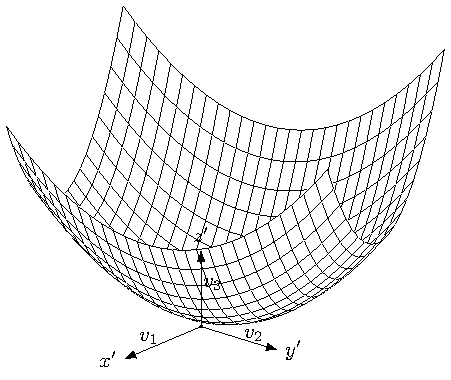
\includegraphics[width=0.7\textwidth]{figuras/6-8-paraboloide-eliptico.pdf}
    \end{figure}

    \subsection*{La prueba de la segunda derivada para funciones de varias variables}

    Consideramos ahora una aplicación de la teoría de las formas cuadráticas al cálculo de varias variables: la deducción de la prueba de la segunda derivada para extremos locales de una función de varias variables. Suponemos cierta familiaridad con el cálculo de funciones de varias variables, en la medida del teorema de Taylor. El lector estará sin duda familiarizado con la versión de una variable de dicho teorema; para un enunciado y una demostración de la versión de varias variables, puede consultarse cualquier texto estándar de cálculo avanzado o análisis.

    Sea $z=f(t_1,t_2,\dots,t_n)$ una función real fija de $n$ variables reales, para la cual existen y son continuas las derivadas parciales de tercer orden. Decimos que $f$ tiene un \textbf{máximo local} en un punto $p\in\R^n$ si existe $\delta>0$ tal que $f(p)\geq f(x)$ siempre que $\norm{x-p}<\delta$. Análogamente, $f$ tiene un \textbf{mínimo local} en $p\in\R^n$ si existe $\delta>0$ tal que $f(p)\leq f(x)$ siempre que $\norm{x-p}<\delta$. Si $f$ tiene un mínimo local o un máximo local en $p$, decimos que $f$ tiene un \textbf{extremo local} en $p$. Un punto $p\in\R^n$ se llama un \textbf{punto crítico} de $f$ si $\partial f(p)/\partial t_i=0$ para $i=1,2,\dots,n$. Es un hecho bien conocido que, si $f$ tiene un extremo local en un punto $p\in\R^n$, entonces $p$ es un punto crítico de $f$. En efecto, si $f$ tiene un extremo local en $p=(p_1,p_2,\dots,p_n)$, entonces, para cualquier $i=1,2,\dots,n$, la función $\phi_i$ definida por $\phi_i(t)=f(p_1,p_2,\dots,p_{i-1},t,p_{i+1},\dots,p_n)$ tiene un extremo local en $t=p_i$. Así, por un argumento elemental de una sola variable,
    \begin{equation*}
        \frac{\partial f(p)}{\partial t_i}=\frac{d\phi_i(p_i)}{dt}=0.
    \end{equation*}
    Así $p$ es un punto crítico de $f$. Pero no todo punto crítico es necesariamente un extremo local.

    Las derivadas parciales de segundo orden de $f$ en un punto crítico $p$ suelen usarse para determinar si $f$ tiene un extremo local en $p$. Estas parciales determinan una matriz $A(p)$ en la cual la entrada del renglón $i$, columna $j$ es
    \begin{equation*}
        \frac{\partial^2f(p)}{(\partial t_i)(\partial t_j)}.
    \end{equation*}
    A esta matriz se le llama la \textbf{matriz hessiana} de $f$ en $p$. Notemos que, si las parciales mixtas de tercer orden de $f$ son continuas, entonces las parciales de segundo orden mixtas de $f$ en $p$ son independientes del orden en que se toman, y por tanto $A(p)$ es una matriz simétrica. En este caso, todos los valores propios de $A(p)$ son reales.

    \begin{teorema}[Prueba de la segunda derivada]
        Sea $f(t_1,t_2,\dots,t_n)$ una función real de $n$ variables reales para la cual todas las derivadas parciales de tercer orden existen y son continuas. Sea $p=(p_1,p_2,\dots,p_n)$ un punto crítico de $f$, y sea $A(p)$ la matriz hessiana de $f$ en $p$.
        \begin{enumerate}[label=(\alph*)]
            \item Si todos los valores propios de $A(p)$ son positivos, entonces $f$ tiene un mínimo local en $p$.
            \item Si todos los valores propios de $A(p)$ son negativos, entonces $f$ tiene un máximo local en $p$.
            \item Si $A(p)$ tiene al menos un valor propio positivo y al menos uno negativo, entonces $f$ no tiene extremo local en $p$ ($p$ se llama un \textbf{punto silla} de $f$).
            \item Si $\rg(A(p))<n$ y $A(p)$ no tiene simultáneamente valores propios positivos y negativos, entonces la prueba de la segunda derivada no es concluyente.
        \end{enumerate}
    \end{teorema}

    \begin{proof}
        Si $p\neq0$, podemos definir una función $g:\R^n\to\R$ por
        \begin{equation*}
            g(t_1,t_2,\dots,t_n)=f(t_1+p_1,t_2+p_2,\dots,t_n+p_n)-f(p).
        \end{equation*}
        Se verifican fácilmente los siguientes hechos:
        \begin{enumerate}
            \item La función $f$ tiene un máximo (mínimo) local en $p$ si y solo si $g$ tiene un máximo (mínimo) local en $0=(0,0,\dots,0)$.
            \item Las derivadas parciales de $g$ en $0$ son iguales a las derivadas parciales correspondientes de $f$ en $p$.
            \item $0$ es un punto crítico de $g$.
            \item $A_{ij}(p)=\dfrac{\partial^2g(0)}{(\partial t_i)(\partial t_j)}$ para todos $i,j$.
        \end{enumerate}
        En vista de estos hechos, podemos suponer, sin pérdida de generalidad, que $p=0$ y $f(p)=0$.

        Aplicamos ahora el teorema de Taylor a $f$ para obtener la aproximación de primer orden de $f$ alrededor de $0$. Tenemos
        \begin{align*}
            f(t_1,t_2,\dots,t_n)&=f(0)+\sum_{i=1}^{n}\frac{\partial f(0)}{\partial t_i}t_i+\frac12\sum_{i,j=1}^{n}\frac{\partial^2f(0)}{(\partial t_i)(\partial t_j)}t_it_j+S(t_1,t_2,\dots,t_n)\\
            &=\frac12\sum_{i,j=1}^{n}\frac{\partial^2f(0)}{(\partial t_i)(\partial t_j)}t_it_j+S(t_1,t_2,\dots,t_n), \tag{13}
        \end{align*}
        donde $S$ es una función real en $\R^n$ tal que
        \begin{equation*}
            \lim_{x\to0}\frac{S(x)}{\norm{x}^2}=\lim_{(t_1,\dots,t_n)\to0}\frac{S(t_1,t_2,\dots,t_n)}{t_1^2+t_2^2+\cdots+t_n^2}=0. \tag{14}
        \end{equation*}
        (En la primera igualdad de (13) usamos que $f(0)=0$ y que las primeras derivadas parciales de $f$ en $0$ son cero, pues $0$ es un punto crítico.)

        Sea $K:\R^n\to\R$ la forma cuadrática definida por
        \begin{equation*}
            K\begin{pmatrix}t_1\\t_2\\\vdots\\t_n\end{pmatrix}=\frac12\sum_{i,j=1}^{n}\frac{\partial^2f(0)}{(\partial t_i)(\partial t_j)}t_it_j, \tag{15}
        \end{equation*}
        sea $H$ la forma bilineal simétrica correspondiente a $K$, y sea $\BB$ la base canónica ordenada de $\R^n$. Es fácil verificar que $\psi_{\BB}(H)=\frac12A(p)$. Como $A(p)$ es simétrica, por el teorema visto en la Sección~6.5 existe una matriz ortogonal $Q$ tal que
        \begin{equation*}
            Q^tA(p)Q=\begin{pmatrix}\lambda_1&0&\cdots&0\\0&\lambda_2&\cdots&0\\\vdots&\vdots&&\vdots\\0&0&\cdots&\lambda_n\end{pmatrix}
        \end{equation*}
        es una matriz diagonal cuyas entradas diagonales son los valores propios de $A(p)$. Sea $\gamma=\{v_1,v_2,\dots,v_n\}$ la base ortogonal de $\R^n$ cuyo $i$-ésimo vector es la $i$-ésima columna de $Q$. Entonces $Q$ es la matriz de cambio de coordenadas que cambia coordenadas relativas a $\gamma$ en coordenadas relativas a $\BB$, y, por el teorema visto anteriormente en esta sección,
        \begin{equation*}
            \psi_\gamma(H)=Q^t\psi_{\BB}(H)Q=\frac12Q^tA(p)Q=\begin{pmatrix}\frac{\lambda_1}{2}&0&\cdots&0\\0&\frac{\lambda_2}{2}&\cdots&0\\\vdots&\vdots&&\vdots\\0&0&\cdots&\frac{\lambda_n}{2}\end{pmatrix}.
        \end{equation*}

        Supongamos que $A(p)$ no es la matriz cero. Entonces $A(p)$ tiene valores propios no nulos. Elijamos $\epsilon>0$ tal que $\epsilon<|\lambda_i|/2$ para todo $\lambda_i\neq0$. Por (14), existe $\delta>0$ tal que, para cualquier $x\in\R^n$ que satisfaga $0<\norm{x}<\delta$, tenemos $|S(x)|<\epsilon\norm{x}^2$. Consideremos cualquier $x\in\R^n$ tal que $0<\norm{x}<\delta$. Entonces, por (13) y (15),
        \begin{equation*}
            |f(x)-K(x)|=|S(x)|<\epsilon\norm{x}^2,
        \end{equation*}
        y por tanto
        \begin{equation*}
            K(x)-\epsilon\norm{x}^2<f(x)<K(x)+\epsilon\norm{x}^2. \tag{16}
        \end{equation*}
        Supongamos que $x=\sum_{i=1}^{n}s_iv_i$. Entonces
        \begin{equation*}
            \norm{x}^2=\sum_{i=1}^{n}s_i^2 \qquad\text{y}\qquad K(x)=\frac12\sum_{i=1}^{n}\lambda_is_i^2,
        \end{equation*}
        por el corolario visto anteriormente en esta sección. Combinando estas ecuaciones con (16), obtenemos
        \begin{equation*}
            \sum_{i=1}^{n}\left(\frac12\lambda_i-\epsilon\right)s_i^2<f(x)<\sum_{i=1}^{n}\left(\frac12\lambda_i+\epsilon\right)s_i^2. \tag{17}
        \end{equation*}

        Supongamos ahora que todos los valores propios de $A(p)$ son positivos. Entonces $\frac12\lambda_i-\epsilon>0$ para todo $i$, y por tanto, por la desigualdad izquierda de (17),
        \begin{equation*}
            f(0)=0\leq\sum_{i=1}^{n}\left(\frac12\lambda_i-\epsilon\right)s_i^2<f(x).
        \end{equation*}
        Así $f(0)\leq f(x)$ para $\norm{x}<\delta$, y por tanto $f$ tiene un mínimo local en $0$. Por un argumento similar usando la desigualdad derecha de (17), si todos los valores propios de $A(p)$ son negativos, entonces $f$ tiene un máximo local en $0$. Esto establece (a) y (b) del teorema.

        A continuación, supongamos que $A(p)$ tiene tanto un valor propio positivo como uno negativo, digamos $\lambda_i>0$ y $\lambda_j<0$ para algunos $i,j$. Entonces $\frac12\lambda_i-\epsilon>0$ y $\frac12\lambda_j+\epsilon<0$. Sea $s$ cualquier número real tal que $0<|s|<\delta$. Sustituyendo $x=sv_i$ y $x=sv_j$ en la desigualdad izquierda y la desigualdad derecha de (17), respectivamente, obtenemos
        \begin{equation*}
            f(0)=0<\left(\frac12\lambda_i-\epsilon\right)s^2<f(sv_i) \qquad\text{y}\qquad f(sv_j)<\left(\frac12\lambda_j+\epsilon\right)s^2<0=f(0).
        \end{equation*}
        Así $f$ toma tanto valores positivos como negativos arbitrariamente cerca de $0$; por tanto $f$ no tiene ni un máximo local ni un mínimo local en $0$. Esto establece (c).

        Para mostrar que la prueba de la segunda derivada es inconcluyente bajo las condiciones enunciadas en (d), consideremos las funciones
        \begin{equation*}
            f(t_1,t_2)=t_1^2-t_2^4 \qquad\text{y}\qquad g(t_1,t_2)=t_1^2+t_2^4
        \end{equation*}
        en $p=0$. En ambos casos, la función tiene un punto crítico en $p$, y
        \begin{equation*}
            A(p)=\begin{pmatrix}2&0\\0&0\end{pmatrix}.
        \end{equation*}
        Sin embargo, $f$ no tiene un extremo local en $0$, mientras que $g$ tiene un mínimo local en $0$.
    \end{proof}

    \subsection*{La ley de inercia de Sylvester}

    Dos representaciones matriciales cualesquiera de una forma bilineal tienen el mismo rango, pues el rango se preserva bajo congruencia. Podemos entonces definir el \textbf{rango} de una forma bilineal como el rango de cualquiera de sus representaciones matriciales. Si una representación matricial es una matriz diagonal, entonces el rango es igual al número de entradas diagonales no nulas de la matriz.

    Restringimos nuestro análisis a las formas bilineales simétricas sobre espacios vectoriales reales de dimensión finita. Toda forma de este tipo tiene una representación matricial diagonal en la cual las entradas diagonales pueden ser positivas, negativas o cero. Aunque estas entradas no son únicas, mostramos que el número de entradas que son positivas y el número que son negativas sí lo son. Es decir, son independientes de la elección de la representación diagonal. A este resultado se le llama la \textit{ley de inercia de Sylvester}. Probamos la ley y la aplicamos para describir las clases de equivalencia de las matrices reales simétricas congruentes.

    \begin{teorema}[Ley de inercia de Sylvester]
        Sea $H$ una forma bilineal simétrica en un espacio vectorial real de dimensión finita $V$. Entonces el número de entradas diagonales positivas y el número de entradas diagonales negativas, en cualquier representación matricial diagonal de $H$, son cada uno independientes de la representación diagonal.
    \end{teorema}

    \begin{proof}
        Supongamos que $\BB$ y $\gamma$ son bases ordenadas de $V$ que determinan representaciones diagonales de $H$. Sin pérdida de generalidad, podemos suponer que $\BB$ y $\gamma$ están ordenadas de modo que, en cada representación diagonal, las entradas están en el orden de positivas, negativas y cero. Basta mostrar que ambas representaciones tienen el mismo número de entradas positivas, porque el número de entradas negativas es igual a la diferencia entre el rango y el número de entradas positivas. Sean $p$ y $q$ el número de entradas diagonales positivas en las representaciones matriciales de $H$ respecto a $\BB$ y $\gamma$, respectivamente. Supongamos que $p\neq q$, y lleguemos a una contradicción. Sin pérdida de generalidad, supongamos que $p<q$. Sean
        \begin{equation*}
            \BB=\{v_1,v_2,\dots,v_p,\dots,v_r,\dots,v_n\} \qquad\text{y}\qquad \gamma=\{w_1,w_2,\dots,w_q,\dots,w_r,\dots,w_n\},
        \end{equation*}
        donde $r$ es el rango de $H$ y $n=\dim(V)$. Sea $L:V\to\R^{p+r-q}$ la función definida por
        \begin{equation*}
            L(x)=(H(x,v_1),H(x,v_2),\dots,H(x,v_p),H(x,w_{q+1}),\dots,H(x,w_r)).
        \end{equation*}
        Se verifica fácilmente que $L$ es lineal, y $\rg(L)\leq p+r-q$. Por tanto
        \begin{equation*}
            \nul(L)\geq n-(p+r-q)>n-r.
        \end{equation*}
        Así, existe un vector no nulo $v_0$ tal que $v_0\notin\gen{\{v_{r+1},v_{r+2},\dots,v_n\}}$, pero $v_0\in\ker(L)$. Como $v_0\in\ker(L)$, se sigue que $H(v_0,v_i)=0$ para $i\leq p$ y $H(v_0,w_i)=0$ para $q<i\leq r$. Supongamos que
        \begin{equation*}
            v_0=\sum_{j=1}^{n}a_jv_j=\sum_{j=1}^{n}b_jw_j.
        \end{equation*}
        Para cualquier $i\leq p$,
        \begin{equation*}
            H(v_0,v_i)=H\left(\sum_{j=1}^{n}a_jv_j,v_i\right)=\sum_{j=1}^{n}a_jH(v_j,v_i)=a_iH(v_i,v_i).
        \end{equation*}
        Pero, para $i\leq p$, tenemos $H(v_i,v_i)>0$ y $H(v_0,v_i)=0$, así que $a_i=0$. Análogamente, $b_i=0$ para $q+1\leq i\leq r$. Como $v_0$ no está en el generado de $\{v_{r+1},v_{r+2},\dots,v_n\}$, se sigue que $a_i\neq0$ para algún $p<i\leq r$. Así
        \begin{equation*}
            H(v_0,v_0)=H\left(\sum_{j=1}^{n}a_jv_j,\sum_{i=1}^{n}a_iv_i\right)=\sum_{j=1}^{n}a_j^2H(v_j,v_j)=\sum_{j=p+1}^{r}a_j^2H(v_j,v_j)<0.
        \end{equation*}
        Más aún,
        \begin{equation*}
            H(v_0,v_0)=H\left(\sum_{j=1}^{n}b_jw_j,\sum_{i=1}^{n}b_iw_i\right)=\sum_{j=1}^{n}b_j^2H(w_j,w_j)=\sum_{j=q+1}^{r}b_j^2H(w_j,w_j)\geq0.
        \end{equation*}
        Así $H(v_0,v_0)<0$ y $H(v_0,v_0)\geq0$, lo cual es una contradicción. Concluimos que $p=q$.
    \end{proof}

    \begin{definicion}[Índice y signatura]
        Al número de entradas diagonales positivas en una representación diagonal de una forma bilineal simétrica sobre un espacio vectorial real se le llama el \textbf{índice} de la forma. A la diferencia entre el número de entradas diagonales positivas y negativas en una representación diagonal de una forma bilineal simétrica se le llama la \textbf{signatura} de la forma. A los tres términos rango, índice y signatura se les llama los \textbf{invariantes} de la forma bilineal, porque son invariantes respecto a las representaciones matriciales. Estos mismos términos se aplican a la forma cuadrática asociada. Notemos que los valores de dos cualesquiera de estos invariantes determinan el valor del tercero.
    \end{definicion}

    \begin{ejemplo}
        La forma bilineal correspondiente a la forma cuadrática $K$ de un ejemplo anterior tiene una representación matricial diagonal $3\times3$ con entradas diagonales $2$, $7$ y $0$. Por tanto, el rango, el índice y la signatura de $K$ son, cada uno, $2$.
    \end{ejemplo}

    \begin{ejemplo}
        La representación matricial de la forma bilineal correspondiente a la forma cuadrática $K(x,y)=x^2-y^2$ en $\R^2$, respecto a la base canónica ordenada, es la matriz diagonal con entradas diagonales $1$ y $-1$. Por tanto, el rango de $K$ es $2$, el índice de $K$ es $1$, y la signatura de $K$ es $0$.
    \end{ejemplo}

    Como la relación de congruencia está íntimamente asociada con las formas bilineales, podemos aplicar la ley de inercia de Sylvester para estudiar esta relación sobre el conjunto de las matrices reales simétricas. Sea $A$ una matriz simétrica $n\times n$, y supongamos que $D$ y $E$ son matrices diagonales congruentes a $A$. Por el corolario visto anteriormente en esta sección, $A$ es la representación matricial de la forma bilineal $H$ en $\R^n$ definida por $H(x,y)=x^tAy$, respecto a la base canónica ordenada de $\R^n$. Por tanto, la ley de inercia de Sylvester nos dice que $D$ y $E$ tienen el mismo número de entradas diagonales positivas y negativas. Podemos enunciar este resultado como la versión matricial de la ley de Sylvester.

    \begin{corolario}[Ley de inercia de Sylvester para matrices]
        Sea $A$ una matriz real simétrica. Entonces el número de entradas diagonales positivas y el número de entradas diagonales negativas, en cualquier matriz diagonal congruente a $A$, son independientes de la elección de la matriz diagonal.
    \end{corolario}

    \begin{definicion}[Índice y signatura de una matriz]
        Sea $A$ una matriz real simétrica, y sea $D$ una matriz diagonal congruente a $A$. Al número de entradas diagonales positivas de $D$ se le llama el \textbf{índice} de $A$. A la diferencia entre el número de entradas diagonales positivas y el número de entradas diagonales negativas de $D$ se le llama la \textbf{signatura} de $A$. Como antes, al rango, el índice y la signatura de una matriz se les llama los \textbf{invariantes} de la matriz, y los valores de dos cualesquiera de estos invariantes determinan el valor del tercero.
    \end{definicion}

    Cualquiera de estos invariantes puede usarse para determinar una clase de equivalencia de matrices reales simétricas congruentes.

    \begin{corolario}
        Dos matrices reales simétricas $n\times n$ son congruentes si y solo si tienen los mismos invariantes.
    \end{corolario}

    \begin{proof}
        Si $A$ y $B$ son matrices simétricas $n\times n$ congruentes, entonces ambas son congruentes a la misma matriz diagonal, y se sigue que tienen los mismos invariantes.

        Recíprocamente, supongamos que $A$ y $B$ son matrices simétricas $n\times n$ con los mismos invariantes. Sean $D$ y $E$ matrices diagonales congruentes a $A$ y $B$, respectivamente, elegidas de modo que las entradas diagonales estén en el orden de positivas, negativas y cero. Como $A$ y $B$ tienen los mismos invariantes, también los tienen $D$ y $E$. Sean $p$ y $r$ el índice y el rango, respectivamente, tanto de $D$ como de $E$. Sea $d_i$ la $i$-ésima entrada diagonal de $D$, y sea $Q$ la matriz diagonal $n\times n$ cuya $i$-ésima entrada diagonal $q_i$ está dada por
        \begin{equation*}
            q_i=\begin{cases}\dfrac{1}{\sqrt{d_i}}&\text{si }1\leq i\leq p\\[1ex]\dfrac{1}{\sqrt{-d_i}}&\text{si }p<i\leq r\\[1ex]1&\text{si }r<i.\end{cases}
        \end{equation*}
        Entonces $Q^tDQ=J_{pr}$, donde
        \begin{equation*}
            J_{pr}=\begin{pmatrix}I_p&O&O\\O&-I_{r-p}&O\\O&O&O\end{pmatrix}.
        \end{equation*}
        Se sigue que $A$ es congruente a $J_{pr}$. Análogamente, $B$ es congruente a $J_{pr}$, y por tanto $A$ es congruente a $B$.
    \end{proof}

    A la matriz $J_{pr}$ se le llama una \textbf{forma canónica} para la teoría de matrices reales simétricas. El siguiente corolario, cuya demostración está contenida en la del corolario anterior, describe el papel de $J_{pr}$.

    \begin{corolario}
        Una matriz real simétrica $n\times n$ $A$ tiene índice $p$ y rango $r$ si y solo si $A$ es congruente a $J_{pr}$ (según se definió arriba).
    \end{corolario}

    \begin{proof}
        Sea $D$ una matriz diagonal congruente a $A$, con las entradas diagonales en el orden de positivas, negativas y cero, y tomemos $Q$ como en la demostración del corolario anterior, de modo que $Q^tDQ=J_{pr}$, donde $p$ y $r$ son el índice y el rango de $A$ (pues $D$, al ser congruente a $A$, tiene los mismos invariantes que $A$). Como la congruencia es transitiva, $A$ es congruente a $J_{pr}$. Recíprocamente, si $A$ es congruente a $J_{p'r'}$ para algún índice $p'$ y rango $r'$, entonces, como la congruencia preserva los invariantes, $A$ tiene índice $p'$ y rango $r'$; en particular, si $A$ tiene índice $p$ y rango $r$, y es congruente a $J_{p'r'}$, entonces $p'=p$ y $r'=r$.
    \end{proof}

    \begin{ejemplo}
        Sean
        \begin{equation*}
            A=\begin{pmatrix}1&-1&3\\-1&2&1\\3&1&1\end{pmatrix}, \qquad B=\begin{pmatrix}1&2&1\\2&3&2\\1&2&1\end{pmatrix}, \qquad\text{y}\qquad C=\begin{pmatrix}1&0&1\\0&1&2\\1&2&1\end{pmatrix}.
        \end{equation*}
        Aplicamos el corolario anterior para determinar cuáles pares de las matrices $A$, $B$ y $C$ son congruentes.

        La matriz $A$ es la matriz de un ejemplo anterior de esta sección, donde se muestra que $A$ es congruente a una matriz diagonal con entradas diagonales $1$, $1$ y $-24$. Por tanto, $A$ tiene rango $3$ e índice $2$. Usando los métodos de dicho ejemplo (no es necesario calcular $Q$), puede mostrarse que $B$ y $C$ son congruentes, respectivamente, a las matrices diagonales
        \begin{equation*}
            \begin{pmatrix}1&0&0\\0&-1&0\\0&0&-1\end{pmatrix} \qquad\text{y}\qquad \begin{pmatrix}1&0&0\\0&1&0\\0&0&-4\end{pmatrix}.
        \end{equation*}
        Se sigue que tanto $A$ como $C$ tienen rango $3$ e índice $2$, mientras que $B$ tiene rango $3$ e índice $1$. Concluimos que $A$ y $C$ son congruentes, pero que $B$ no es congruente ni a $A$ ni a $C$.
    \end{ejemplo}

    \section{La teoría especial de la relatividad de Einstein}

    Como consecuencia de experimentos físicos realizados en la segunda mitad del siglo XIX (el más notable, el experimento de Michelson--Morley de 1887), los físicos concluyeron que \textit{los resultados obtenidos al medir la velocidad de la luz son independientes de la velocidad del instrumento usado para medirla}. Por ejemplo, supongamos que, en la Tierra, un experimentador mide la velocidad de la luz emitida por el Sol y encuentra que es de $186\,000$ millas por segundo. Supongamos ahora que el experimentador coloca el equipo de medición en una nave espacial que sale de la Tierra viajando a $100\,000$ millas por segundo en una dirección que se aleja del Sol. Al repetir el mismo experimento desde la nave espacial se obtiene el mismo resultado: la luz viaja a $186\,000$ millas por segundo relativas a la nave espacial, ¡en vez de las $86\,000$ millas por segundo que uno esperaría!

    Esta revelación llevó a una nueva manera de relacionar los sistemas de coordenadas usados para ubicar eventos en el espacio-tiempo. El resultado fue la \textit{teoría especial de la relatividad} de Albert Einstein. En esta sección desarrollamos, desde el punto de vista del álgebra lineal, la esencia de la teoría de Einstein.

    El problema básico es comparar dos sistemas de coordenadas inerciales (no acelerados) distintos, $S$ y $S'$, en el espacio tridimensional ($\R^3$), que están en movimiento relativo entre sí, bajo el supuesto de que la velocidad de la luz es la misma medida en cualquiera de los dos sistemas. Suponemos que $S'$ se mueve a velocidad constante en relación con $S$, según se mide desde $S$. (Véase la siguiente figura.) Para simplificar las cosas, supongamos que se cumplen las siguientes condiciones:
    \begin{enumerate}
        \item Los ejes correspondientes de $S$ y $S'$ ($x$ y $x'$, $y$ y $y'$, $z$ y $z'$) son paralelos, y el origen de $S'$ se mueve en la dirección positiva del eje $x$ de $S$ a una velocidad constante $v>0$ relativa a $S$.
        \item Dos relojes $C$ y $C'$ se colocan en el espacio: el primero estacionario respecto al sistema de coordenadas $S$, y el segundo estacionario respecto al sistema de coordenadas $S'$. Estos relojes están diseñados para dar números reales como lecturas, en unidades de segundos. Los relojes se calibran de modo que, en el instante en que los orígenes de $S$ y $S'$ coinciden, ambos relojes marcan cero.
        \item La unidad de longitud es el \textbf{segundo luz} (la distancia que recorre la luz en $1$ segundo), y la unidad de tiempo es el segundo. Notemos que, con estas unidades, la velocidad de la luz es $1$ segundo luz por segundo.
    \end{enumerate}

    \begin{figure}[H]
        \centering
        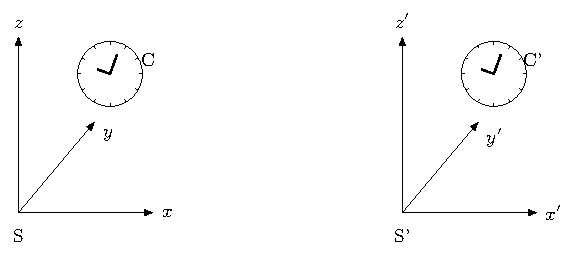
\includegraphics[width=0.85\textwidth]{figuras/sistemas-coordenados-relatividad.pdf}
    \end{figure}

    Dado cualquier evento (algo cuya posición y momento de ocurrencia pueden describirse), podemos asignarle un conjunto de \textit{coordenadas espacio-temporales}. Por ejemplo, si $p$ es un evento que ocurre en la posición
    \begin{equation*}
        \begin{pmatrix}x\\y\\z\end{pmatrix}
    \end{equation*}
    relativa a $S$ y en el tiempo $t$ leído en el reloj $C$, podemos asignar a $p$ el conjunto de coordenadas
    \begin{equation*}
        \begin{pmatrix}x\\y\\z\\t\end{pmatrix}.
    \end{equation*}
    A esta $4$-tupla ordenada se le llama las \textbf{coordenadas espacio-temporales} de $p$ relativas a $S$ y $C$. Análogamente, $p$ tiene un conjunto de coordenadas espacio-temporales
    \begin{equation*}
        \begin{pmatrix}x'\\y'\\z'\\t'\end{pmatrix}
    \end{equation*}
    relativas a $S'$ y $C'$.

    Para una velocidad fija $v$, sea $T_v:\R^4\to\R^4$ la función definida por
    \begin{equation*}
        T_v\begin{pmatrix}x\\y\\z\\t\end{pmatrix}=\begin{pmatrix}x'\\y'\\z'\\t'\end{pmatrix},
    \end{equation*}
    donde
    \begin{equation*}
        \begin{pmatrix}x\\y\\z\\t\end{pmatrix} \qquad\text{y}\qquad \begin{pmatrix}x'\\y'\\z'\\t'\end{pmatrix}
    \end{equation*}
    son las coordenadas espacio-temporales del mismo evento respecto a $S$ y $C$, y respecto a $S'$ y $C'$, respectivamente. Einstein hizo ciertos supuestos sobre $T_v$ que lo llevaron a su teoría especial de la relatividad. Formulamos un conjunto equivalente de supuestos.

    \subsection*{Axiomas de la teoría especial de la relatividad}

    \begin{description}
        \item[(R1)] La velocidad de cualquier haz de luz, medida en cualquiera de los dos sistemas de coordenadas usando un reloj estacionario relativo a ese sistema de coordenadas, es $1$.
        \item[(R2)] La función $T_v:\R^4\to\R^4$ es un isomorfismo.
        \item[(R3)] Si
        \begin{equation*}
            T_v\begin{pmatrix}x\\y\\z\\t\end{pmatrix}=\begin{pmatrix}x'\\y'\\z'\\t'\end{pmatrix},
        \end{equation*}
        entonces $y'=y$ y $z'=z$.
        \item[(R4)] Si
        \begin{equation*}
            T_v\begin{pmatrix}x\\y_1\\z_1\\t\end{pmatrix}=\begin{pmatrix}x'\\y'\\z'\\t'\end{pmatrix} \qquad\text{y}\qquad T_v\begin{pmatrix}x\\y_2\\z_2\\t\end{pmatrix}=\begin{pmatrix}x''\\y''\\z''\\t''\end{pmatrix},
        \end{equation*}
        entonces $x''=x'$ y $t''=t'$.
        \item[(R5)] El origen de $S$ se mueve en la dirección negativa del eje $x'$ de $S'$ a la velocidad constante $-v<0$, medida desde $S'$.
    \end{description}

    Los axiomas (R3) y (R4) nos dicen que, para $p\in\R^4$, la segunda y tercera coordenadas de $T_v(p)$ no cambian, y que la primera y cuarta coordenadas de $T_v(p)$ son independientes de la segunda y tercera coordenadas de $p$.

    Como veremos, estos cinco axiomas caracterizan por completo a $T_v$. Al operador $T_v$ se le llama la \textbf{transformación de Lorentz} en la dirección $x$. Nos proponemos calcular $T_v$ y usarla para estudiar el curioso fenómeno de la contracción del tiempo.

    \begin{teorema}
        En $\R^4$, se cumple lo siguiente:
        \begin{enumerate}[label=(\alph*)]
            \item $T_v(e_i)=e_i$ para $i=2,3$.
            \item $\gen{\{e_2,e_3\}}$ es $T_v$-invariante.
            \item $\gen{\{e_1,e_4\}}$ es $T_v$-invariante.
            \item Tanto $\gen{\{e_2,e_3\}}$ como $\gen{\{e_1,e_4\}}$ son $T_v^*$-invariantes.
            \item $T_v^*(e_i)=e_i$ para $i=2,3$.
        \end{enumerate}
    \end{teorema}

    \begin{proof}
        (a) Por el axioma (R2), $T_v$ es lineal (por ser un isomorfismo), y por tanto
        \begin{equation*}
            T_v\begin{pmatrix}0\\0\\0\\0\end{pmatrix}=\begin{pmatrix}0\\0\\0\\0\end{pmatrix},
        \end{equation*}
        y por tanto, por el axioma (R4), la primera y cuarta coordenadas de
        \begin{equation*}
            T_v\begin{pmatrix}0\\a\\b\\0\end{pmatrix}
        \end{equation*}
        son ambas cero para cualesquiera $a,b\in\R$. Así, por el axioma (R3),
        \begin{equation*}
            T_v\begin{pmatrix}0\\1\\0\\0\end{pmatrix}=\begin{pmatrix}0\\1\\0\\0\end{pmatrix} \qquad\text{y}\qquad T_v\begin{pmatrix}0\\0\\1\\0\end{pmatrix}=\begin{pmatrix}0\\0\\1\\0\end{pmatrix},
        \end{equation*}
        es decir, $T_v(e_2)=e_2$ y $T_v(e_3)=e_3$.

        (b) Sea $w=(0,a,b,0)\in\gen{\{e_2,e_3\}}$. Por el axioma (R3), las coordenadas segunda y tercera de $T_v(w)$ son $a$ y $b$, respectivamente. Como $w$ tiene primera y cuarta coordenadas iguales a $0$, y las de $T_v(0,0,0,0)=(0,0,0,0)$ (por (a) del razonamiento anterior, con $T_v$ lineal) también son $0$, el axioma (R4) implica que la primera y cuarta coordenadas de $T_v(w)$ coinciden con las de $T_v(0,0,0,0)=0$, es decir, son ambas $0$. Así $T_v(w)=(0,a,b,0)\in\gen{\{e_2,e_3\}}$, lo cual prueba (b).

        (c) Sea $w=(x,0,0,t)\in\gen{\{e_1,e_4\}}$. Por el axioma (R3) (con $y=z=0$), las coordenadas segunda y tercera de $T_v(w)$ son $0$ y $0$. Así $T_v(w)$ tiene la forma $(x',0,0,t')\in\gen{\{e_1,e_4\}}$, lo cual prueba (c).

        (d) Sea $\gamma=\{e_2,e_3,e_1,e_4\}$, una reordenación de la base canónica de $\R^4$, la cual es ortonormal respecto al producto interno estándar. Por (b) y (c), $T_v$ deja invariantes tanto a $\gen{\{e_2,e_3\}}$ como a $\gen{\{e_1,e_4\}}$; así, la matriz $[T_v]_\gamma$ tiene la forma de bloques
        \begin{equation*}
            \begin{pmatrix}P&O\\O&Q\end{pmatrix},
        \end{equation*}
        donde $P$ es $2\times2$ y $Q$ es $2\times2$ (sin términos cruzados, pues cada subespacio se mapea en sí mismo). Por el teorema visto en la Sección~6.3, $[T_v^*]_\gamma=([T_v]_\gamma)^*=\begin{pmatrix}P^*&O\\O&Q^*\end{pmatrix}$, que también tiene esta misma forma de bloques (sin términos cruzados). Por tanto, $T_v^*$ también deja invariantes tanto a $\gen{\{e_2,e_3\}}$ como a $\gen{\{e_1,e_4\}}$, lo cual prueba (d).

        (e) Para cualquier $j\neq2$, $\iprod{T_v^*(e_2)}{e_j}=\iprod{e_2}{T_v(e_j)}=0$ por (a) y (c) (pues, si $j=1$ o $j=4$, $T_v(e_j)\in\gen{\{e_1,e_4\}}$ por (c), el cual es ortogonal a $e_2$; y si $j=3$, $T_v(e_3)=e_3$ por (a), ortogonal a $e_2$); para $j=2$, $\iprod{T_v^*(e_2)}{e_2}=\iprod{e_2}{T_v(e_2)}=\iprod{e_2}{e_2}=1$ por (a). Concluimos que $T_v^*(e_2)$ es un múltiplo de $e_2$ (es decir, que $T_v^*(e_2)=ke_2$ para algún $k\in\R$). Así,
        \begin{equation*}
            1=\iprod{e_2}{e_2}=\iprod{e_2}{T_v(e_2)}=\iprod{T_v^*(e_2)}{e_2}=\iprod{ke_2}{e_2}=k,
        \end{equation*}
        y por tanto $T_v^*(e_2)=e_2$. Análogamente, $T_v^*(e_3)=e_3$.
    \end{proof}

    Supongamos que, en el instante en que coinciden los orígenes de $S$ y $S'$, se emite un destello de luz desde su origen común. El evento del destello de luz, medido tanto relativo a $S$ y $C$ como relativo a $S'$ y $C'$, tiene coordenadas espacio-temporales
    \begin{equation*}
        \begin{pmatrix}0\\0\\0\\0\end{pmatrix}.
    \end{equation*}
    Sea $P$ el conjunto de todos los eventos cuyas coordenadas espacio-temporales
    \begin{equation*}
        \begin{pmatrix}x\\y\\z\\t\end{pmatrix}
    \end{equation*}
    relativas a $S$ y $C$ son tales que el destello es observable desde el punto con coordenadas
    \begin{equation*}
        \begin{pmatrix}x\\y\\z\end{pmatrix}
    \end{equation*}
    (medidas relativas a $S$) en el tiempo $t$ (medido en $C$). Caractericemos a $P$ en términos de $x,y,z$ y $t$. Como la velocidad de la luz es $1$, en cualquier tiempo $t\geq0$ el destello de luz es observable desde cualquier punto cuya distancia al origen de $S$ (medida en $S$) sea $t\cdot1=t$. Estos son precisamente los puntos que se encuentran sobre la esfera de radio $t$ con centro en el origen. Las coordenadas (relativas a $S$) de tales puntos satisfacen la ecuación $x^2+y^2+z^2-t^2=0$. Así, un evento está en $P$ si y solo si sus coordenadas espacio-temporales
    \begin{equation*}
        \begin{pmatrix}x\\y\\z\\t\end{pmatrix} \qquad (t\geq0)
    \end{equation*}
    relativas a $S$ y $C$ satisfacen la ecuación $x^2+y^2+z^2-t^2=0$. En virtud del axioma (R1), podemos caracterizar a $P$ en términos de las coordenadas espacio-temporales relativas a $S'$ y $C'$ de manera análoga: un evento está en $P$ si y solo si, relativo a $S'$ y $C'$, sus coordenadas espacio-temporales
    \begin{equation*}
        \begin{pmatrix}x'\\y'\\z'\\t'\end{pmatrix} \qquad (t'\geq0)
    \end{equation*}
    satisfacen la ecuación $(x')^2+(y')^2+(z')^2-(t')^2=0$.

    Sea
    \begin{equation*}
        A=\begin{pmatrix}1&0&0&0\\0&1&0&0\\0&0&1&0\\0&0&0&-1\end{pmatrix}.
    \end{equation*}

    \begin{teorema}
        Si $\iprod{L_A(w)}{w}=0$ para algún $w\in\R^4$, entonces
        \begin{equation*}
            \iprod{T_v^*L_AT_v(w)}{w}=0.
        \end{equation*}
    \end{teorema}

    \begin{proof}
        Sea
        \begin{equation*}
            w=\begin{pmatrix}x\\y\\z\\t\end{pmatrix}\in\R^4,
        \end{equation*}
        y supongamos que $\iprod{L_A(w)}{w}=0$.

        \textbf{Caso 1.} $t\geq0$. Como $\iprod{L_A(w)}{w}=x^2+y^2+z^2-t^2$, el vector $w$ da las coordenadas de un evento en $P$ relativas a $S$ y $C$. Como, según la discusión anterior al teorema, $(x')^2+(y')^2+(z')^2-(t')^2=0$, donde $(x',y',z',t')^t=T_v(w)$ son las coordenadas espacio-temporales del mismo evento relativas a $S'$ y $C'$, tenemos
        \begin{equation*}
            \iprod{T_v^*L_AT_v(w)}{w}=\iprod{L_AT_v(w)}{T_v(w)}=(x')^2+(y')^2+(z')^2-(t')^2=0,
        \end{equation*}
        y se sigue la conclusión.

        \textbf{Caso 2.} $t<0$. La demostración se obtiene aplicando el Caso~1 a $-w$, pues $\iprod{L_A(-w)}{-w}=\iprod{L_A(w)}{w}=0$, y como $L_A,T_v,T_v^*$ son lineales, $\iprod{T_v^*L_AT_v(-w)}{-w}=\iprod{T_v^*L_AT_v(w)}{w}$; así, la conclusión del Caso~1 aplicada a $-w$ (cuya cuarta coordenada $-t$ es $\geq0$) da el resultado para $w$.
    \end{proof}

    Procedemos ahora a deducir información sobre $T_v$. Sean
    \begin{equation*}
        w_1=\begin{pmatrix}1\\0\\0\\1\end{pmatrix} \qquad\text{y}\qquad w_2=\begin{pmatrix}1\\0\\0\\-1\end{pmatrix}.
    \end{equation*}
    Por el inciso (c) del teorema anterior, $\{w_1,w_2\}$ es una base ortogonal de $\gen{\{e_1,e_4\}}$, y por (d) del mismo teorema, $\gen{\{e_1,e_4\}}$ es $T_v^*L_AT_v$-invariante (pues es tanto $T_v$-invariante como $T_v^*$-invariante, y $L_A$ claramente deja invariante a $\gen{\{e_1,e_4\}}$, ya que $A$ es diagonal). El siguiente resultado nos dice aún más.

    \begin{teorema}
        Existen escalares no nulos $a$ y $b$ tales que
        \begin{enumerate}[label=(\alph*)]
            \item $T_v^*L_AT_v(w_1)=aw_2$.
            \item $T_v^*L_AT_v(w_2)=bw_1$.
        \end{enumerate}
    \end{teorema}

    \begin{proof}
        (a) Como $\iprod{L_A(w_1)}{w_1}=1+0+0-1=0$, se sigue del teorema anterior que $\iprod{T_v^*L_AT_v(w_1)}{w_1}=0$. Como $\gen{\{w_1,w_2\}}=\gen{\{e_1,e_4\}}$ es $T_v^*L_AT_v$-invariante, $T_v^*L_AT_v(w_1)$ debe estar en este subespacio, así que $T_v^*L_AT_v(w_1)=\alpha w_1+\beta w_2$ para ciertos escalares $\alpha,\beta$. Pero
        \begin{equation*}
            0=\iprod{T_v^*L_AT_v(w_1)}{w_1}=\alpha\iprod{w_1}{w_1}+\beta\iprod{w_2}{w_1}=2\alpha+0\cdot\beta=2\alpha
        \end{equation*}
        (usando que $\iprod{w_1}{w_1}=2$ y $\iprod{w_2}{w_1}=1-1=0$), así que $\alpha=0$. Así $T_v^*L_AT_v(w_1)=\beta w_2$ para algún escalar $\beta$. Como $T_v$ y $A$ son invertibles, también lo es $T_v^*L_AT_v$, así que $\beta\neq0$; hacemos $a=\beta$, lo cual prueba (a).

        (b) La demostración es similar a la de (a). Como $\iprod{L_A(w_2)}{w_2}=1+0+0-1=0$, tenemos $\iprod{T_v^*L_AT_v(w_2)}{w_2}=0$ por el teorema anterior. Escribiendo $T_v^*L_AT_v(w_2)=\alpha w_1+\beta w_2$, obtenemos
        \begin{equation*}
            0=\iprod{T_v^*L_AT_v(w_2)}{w_2}=\alpha\iprod{w_1}{w_2}+\beta\iprod{w_2}{w_2}=0\cdot\alpha+2\beta,
        \end{equation*}
        así que $\beta=0$, y $T_v^*L_AT_v(w_2)=\alpha w_1$ para algún $\alpha\neq0$ (por invertibilidad, como en (a)); hacemos $b=\alpha$.
    \end{proof}

    \begin{corolario}
        Sea $B_v=[T_v]_\beta$, donde $\beta$ es la base canónica ordenada de $\R^4$. Entonces:
        \begin{enumerate}[label=(\alph*)]
            \item $B_v^*AB_v$ tiene la forma $\begin{pmatrix}a&0&0&0\\0&1&0&0\\0&0&1&0\\0&0&0&-a\end{pmatrix}$ para algún escalar $a\neq0$.
            \item $T_v^*L_AT_v=aL_A$.
        \end{enumerate}
    \end{corolario}

    \begin{proof}
        Notemos primero que $U=T_v^*L_AT_v$ es autoadjunto, pues $U^*=T_v^*L_A^*T_v^{**}=T_v^*L_AT_v=U$ (usando que $L_A^*=L_A$, pues $A$ es real y diagonal, y por tanto simétrica). Por el teorema anterior, $U(w_1)=aw_2$ y $U(w_2)=bw_1$, con $a,b\neq0$. Por autoadjunción,
        \begin{equation*}
            a\iprod{w_2}{w_2}=\iprod{U(w_1)}{w_2}=\iprod{w_1}{U(w_2)}=b\iprod{w_1}{w_1},
        \end{equation*}
        y como $\iprod{w_1}{w_1}=\iprod{w_2}{w_2}=2$, se sigue que $a=b$.

        Como $w_1=e_1+e_4$ y $w_2=e_1-e_4$, tenemos $e_1=\frac12(w_1+w_2)$ y $e_4=\frac12(w_1-w_2)$. Así,
        \begin{equation*}
            U(e_1)=\frac12(U(w_1)+U(w_2))=\frac12(aw_2+aw_1)=ae_1
        \end{equation*}
        y
        \begin{equation*}
            U(e_4)=\frac12(U(w_1)-U(w_2))=\frac12(aw_2-aw_1)=-ae_4.
        \end{equation*}
        Junto con el teorema anterior de esta sección, que da $U(e_2)=T_v^*L_AT_v(e_2)=T_v^*L_A(e_2)=T_v^*(e_2)=e_2$ (pues $T_v(e_2)=e_2$, $L_A(e_2)=e_2$, y $T_v^*(e_2)=e_2$) y análogamente $U(e_3)=e_3$, concluimos que, en la base canónica,
        \begin{equation*}
            [U]_\beta=[T_v^*L_AT_v]_\beta=B_v^*AB_v=\begin{pmatrix}a&0&0&0\\0&1&0&0\\0&0&1&0\\0&0&0&-a\end{pmatrix}.
        \end{equation*}
        Esto prueba (a). Para (b), notemos que esta matriz es precisamente $aA$; así $B_v^*AB_v=aA$, y por tanto $U=T_v^*L_AT_v=aL_A$, lo cual prueba (b). (Verificaremos, tras calcular $B_v$ explícitamente más adelante, que de hecho $a=1$, y por tanto $B_v^*AB_v=A$.)
    \end{proof}

    Consideremos ahora la situación $1$ segundo después de que los orígenes de $S$ y $S'$ hayan coincidido, medido según el reloj $C$. Como el origen de $S'$ se mueve a lo largo del eje $x$ a una velocidad $v$ medida en $S$, sus coordenadas espacio-temporales relativas a $S$ y $C$ son
    \begin{equation*}
        \begin{pmatrix}v\\0\\0\\1\end{pmatrix}.
    \end{equation*}
    Análogamente, las coordenadas espacio-temporales para el origen de $S'$ relativas a $S'$ y $C'$ deben ser
    \begin{equation*}
        \begin{pmatrix}0\\0\\0\\t'\end{pmatrix}
    \end{equation*}
    para algún $t'>0$. Así tenemos
    \begin{equation*}
        T_v\begin{pmatrix}v\\0\\0\\1\end{pmatrix}=\begin{pmatrix}0\\0\\0\\t'\end{pmatrix} \qquad\text{para algún } t'>0. \tag{18}
    \end{equation*}
    Por el corolario al teorema anterior (con $a=1$; véase la nota al final de su demostración, que confirmaremos más abajo),
    \begin{equation*}
        \iprod{T_v^*L_AT_v\begin{pmatrix}v\\0\\0\\1\end{pmatrix}}{\begin{pmatrix}v\\0\\0\\1\end{pmatrix}}=\iprod{L_A\begin{pmatrix}v\\0\\0\\1\end{pmatrix}}{\begin{pmatrix}v\\0\\0\\1\end{pmatrix}}=v^2-1. \tag{19}
    \end{equation*}
    Pero también
    \begin{align*}
        \iprod{T_v^*L_AT_v\begin{pmatrix}v\\0\\0\\1\end{pmatrix}}{\begin{pmatrix}v\\0\\0\\1\end{pmatrix}}&=\iprod{L_AT_v\begin{pmatrix}v\\0\\0\\1\end{pmatrix}}{T_v\begin{pmatrix}v\\0\\0\\1\end{pmatrix}}\\
        &=\iprod{L_A\begin{pmatrix}0\\0\\0\\t'\end{pmatrix}}{\begin{pmatrix}0\\0\\0\\t'\end{pmatrix}}=-(t')^2. \tag{20}
    \end{align*}
    Combinando (19) y (20), concluimos que $v^2-1=-(t')^2$, o
    \begin{equation*}
        t'=\sqrt{1-v^2}. \tag{21}
    \end{equation*}
    Así, de (18) y (21), obtenemos
    \begin{equation*}
        T_v\begin{pmatrix}v\\0\\0\\1\end{pmatrix}=\begin{pmatrix}0\\0\\0\\\sqrt{1-v^2}\end{pmatrix}. \tag{22}
    \end{equation*}

    A continuación, recordemos que el origen de $S$ se mueve en la dirección negativa del eje $x'$ de $S'$ a la velocidad constante $-v<0$ medida desde $S'$ (axioma (R5)). En consecuencia, $1$ segundo después de que los orígenes de $S$ y $S'$ hayan coincidido, medido en el reloj $C$, existe un tiempo $t''>0$ medido en el reloj $C'$ tal que
    \begin{equation*}
        T_v\begin{pmatrix}0\\0\\0\\1\end{pmatrix}=\begin{pmatrix}-vt''\\0\\0\\t''\end{pmatrix}. \tag{23}
    \end{equation*}
    De (23), se sigue, de manera similar a la deducción de (22), que
    \begin{equation*}
        t''=\frac{1}{\sqrt{1-v^2}}; \tag{24}
    \end{equation*}
    (en efecto, aplicando el mismo argumento usado para obtener (19)-(21), ahora con el vector $(0,0,0,1)^t$ en lugar de $(v,0,0,1)^t$: $\iprod{L_A(0,0,0,1)^t}{(0,0,0,1)^t}=-1$, y por otro lado, usando (23), $\iprod{L_A(-vt'',0,0,t'')^t}{(-vt'',0,0,t'')^t}=v^2(t'')^2-(t'')^2$; igualando, $-1=(t'')^2(v^2-1)$, de donde $(t'')^2=1/(1-v^2)$, y como $t''>0$, se obtiene (24)); así, de (23) y (24),
    \begin{equation*}
        T_v\begin{pmatrix}0\\0\\0\\1\end{pmatrix}=\begin{pmatrix}\dfrac{-v}{\sqrt{1-v^2}}\\[1ex]0\\0\\\dfrac{1}{\sqrt{1-v^2}}\end{pmatrix}. \tag{25}
    \end{equation*}

    El siguiente resultado se prueba ahora fácilmente usando (22), (25) y el teorema visto anteriormente en esta sección (que da $T_v(e_2)=e_2$ y $T_v(e_3)=e_3$).

    \begin{teorema}
        Sea $\beta$ la base canónica ordenada de $\R^4$. Entonces
        \begin{equation*}
            [T_v]_\beta=B_v=\begin{pmatrix}\dfrac{1}{\sqrt{1-v^2}}&0&0&\dfrac{-v}{\sqrt{1-v^2}}\\[1.2ex]0&1&0&0\\0&0&1&0\\[0.3ex]\dfrac{-v}{\sqrt{1-v^2}}&0&0&\dfrac{1}{\sqrt{1-v^2}}\end{pmatrix}.
        \end{equation*}
    \end{teorema}

    \begin{proof}
        De (22), la primera columna de $B_v$ se obtiene despejando $T_v(e_1)$: como $T_v(v,0,0,1)^t=vT_v(e_1)+T_v(e_4)$, y de (25) sabemos $T_v(e_4)$; sustituyendo en (22) y despejando $T_v(e_1)$ se obtiene la primera columna indicada. La cuarta columna es (25). Las columnas segunda y tercera son $T_v(e_2)=e_2$ y $T_v(e_3)=e_3$, por el teorema visto anteriormente en esta sección.

        Verifiquemos explícitamente la primera columna: de (25), $T_v(e_4)=\left(\frac{-v}{\sqrt{1-v^2}},0,0,\frac{1}{\sqrt{1-v^2}}\right)^t$. De (22), $vT_v(e_1)+T_v(e_4)=(0,0,0,\sqrt{1-v^2})^t$, así que
        \begin{equation*}
            vT_v(e_1)=\left(\frac{v}{\sqrt{1-v^2}},0,0,\sqrt{1-v^2}-\frac{1}{\sqrt{1-v^2}}\right)^t=\left(\frac{v}{\sqrt{1-v^2}},0,0,\frac{-v^2}{\sqrt{1-v^2}}\right)^t,
        \end{equation*}
        y dividiendo entre $v$,
        \begin{equation*}
            T_v(e_1)=\left(\frac{1}{\sqrt{1-v^2}},0,0,\frac{-v}{\sqrt{1-v^2}}\right)^t,
        \end{equation*}
        que es la primera columna indicada.

        Finalmente, se verifica por sustitución directa que, con esta $B_v$, $B_v^*AB_v=A$ (es decir, que $a=1$ en el corolario visto anteriormente en esta sección), confirmando la nota hecha en su demostración.
    \end{proof}

    \subsection*{Contracción del tiempo}

    Una conclusión de lo más curiosa y paradójica se sigue si aceptamos la teoría de Einstein. Supongamos que un astronauta sale de nuestro sistema solar en un vehículo espacial que viaja a una velocidad fija $v$ medida en relación con nuestro sistema solar. Se sigue de la teoría de Einstein que, al final de un tiempo $t$ medido en la Tierra, el tiempo que ha transcurrido en el vehículo espacial es solamente $t\sqrt{1-v^2}$. Para establecer este resultado, consideremos los sistemas de coordenadas $S$ y $S'$ y los relojes $C$ y $C'$ que hemos estado estudiando. Supongamos que el origen de $S'$ coincide con el vehículo espacial, y el origen de $S$ coincide con un punto en el sistema solar (estacionario respecto al Sol), de modo que los orígenes de $S$ y $S'$ coinciden y los relojes $C$ y $C'$ marcan cero en el instante en que el astronauta emprende el viaje.

    Como se ve desde $S$, las coordenadas espacio-temporales del vehículo en cualquier tiempo $t>0$ medido por $C$ son
    \begin{equation*}
        \begin{pmatrix}vt\\0\\0\\t\end{pmatrix},
    \end{equation*}
    mientras que, como se ve desde $S'$, las coordenadas espacio-temporales del vehículo en cualquier tiempo $t'>0$ medido por $C'$ son
    \begin{equation*}
        \begin{pmatrix}0\\0\\0\\t'\end{pmatrix}.
    \end{equation*}
    Pero si dos conjuntos de coordenadas espacio-temporales
    \begin{equation*}
        \begin{pmatrix}vt\\0\\0\\t\end{pmatrix} \qquad\text{y}\qquad \begin{pmatrix}0\\0\\0\\t'\end{pmatrix}
    \end{equation*}
    han de describir el mismo evento, debe cumplirse que
    \begin{equation*}
        T_v\begin{pmatrix}vt\\0\\0\\t\end{pmatrix}=\begin{pmatrix}0\\0\\0\\t'\end{pmatrix}.
    \end{equation*}
    Así,
    \begin{equation*}
        [T_v]_\beta=B_v\begin{pmatrix}vt\\0\\0\\t\end{pmatrix}=\begin{pmatrix}0\\0\\0\\t'\end{pmatrix}.
    \end{equation*}
    De la ecuación anterior, obtenemos $\dfrac{-v^2t}{\sqrt{1-v^2}}+\dfrac{t}{\sqrt{1-v^2}}=t'$, o
    \begin{equation*}
        t'=t\sqrt{1-v^2}. \tag{26}
    \end{equation*}
    Este es el resultado deseado.

    Una consecuencia dramática de la contracción del tiempo es que las distancias se contraen a lo largo de la línea de movimiento.

    Hagamos una observación adicional. Supongamos que consideramos unidades de distancia y tiempo más comúnmente usadas que el segundo luz y el segundo, tales como la milla y la hora, o el kilómetro y el segundo. Sea $c$ la velocidad de la luz relativa a nuestras unidades elegidas. Es fácil ver que, si un objeto viaja a una velocidad $v$ relativa a un conjunto de unidades, entonces viaja a una velocidad $v/c$ en unidades de segundos luz por segundo. Así, para un conjunto arbitrario de unidades de distancia y tiempo, (26) se convierte en
    \begin{equation*}
        t'=t\sqrt{1-\frac{v^2}{c^2}}.
    \end{equation*}

\section{Condicionamiento y el cociente de Rayleigh}

En el primer curso estudiamos técnicas específicas que permiten resolver sistemas de ecuaciones lineales de la forma $Ax=b$, donde $A$ es una matriz $m\times n$ y $b$ es un vector $m\times 1$. Tales sistemas surgen con frecuencia en aplicaciones al mundo real. Los coeficientes del sistema suelen obtenerse a partir de datos experimentales y, en muchos casos, tanto $m$ como $n$ son tan grandes que debe usarse una computadora en el cálculo de la solución. Así, deben considerarse dos tipos de errores. Primero, surgen errores experimentales en la recolección de datos, pues ningún instrumento puede proporcionar mediciones completamente exactas. Segundo, las computadoras introducen errores de redondeo. Uno podría sentir intuitivamente que pequeños cambios relativos en los coeficientes del sistema provocan pequeños errores relativos en la solución. Un sistema que tiene esta propiedad se llama \textbf{bien condicionado}; en caso contrario, se llama \textbf{mal condicionado}.

Consideramos ahora varios ejemplos de estos tipos de errores, concentrándonos principalmente en cambios en $b$ en lugar de en las entradas de $A$. Además, suponemos que $A$ es una matriz cuadrada, compleja (o real) e invertible, pues es el caso que se encuentra con más frecuencia en las aplicaciones.

\begin{ejemplo}
    Consideremos el sistema
    \begin{align*}
        x_1+x_2&=5\\
        x_1-x_2&=1.
    \end{align*}
    La solución de este sistema es
    \begin{equation*}
        \begin{pmatrix}3\\2\end{pmatrix}.
    \end{equation*}
    Supongamos ahora que modificamos un poco el sistema y consideramos el nuevo sistema
    \begin{align*}
        x_1+x_2&=5\\
        x_1-x_2&=1.0001.
    \end{align*}
    Este sistema modificado tiene la solución
    \begin{equation*}
        \begin{pmatrix}3.00005\\1.99995\end{pmatrix}.
    \end{equation*}
    Vemos que un cambio de $10^{-4}$ en un coeficiente ha provocado un cambio menor a $10^{-4}$ en cada coordenada de la nueva solución. Más generalmente, el sistema
    \begin{align*}
        x_1+x_2&=5\\
        x_1-x_2&=1+\delta
    \end{align*}
    tiene la solución
    \begin{equation*}
        \begin{pmatrix}3+\delta/2\\2-\delta/2\end{pmatrix}.
    \end{equation*}
    Así, pequeños cambios en $b$ introducen pequeños cambios en la solución. Por supuesto, en realidad nos interesan los \textit{cambios relativos}, pues un cambio en la solución de, digamos, $10$ se considera grande si la solución original es del orden $10^{-2}$, pero pequeño si la solución original es del orden $10^{6}$.

    Usamos la notación $\delta b$ para denotar el vector $b'-b$, donde $b$ es el vector del sistema original y $b'$ es el vector del sistema modificado. Así, en este caso,
    \begin{equation*}
        \delta b=\begin{pmatrix}5\\1+h\end{pmatrix}-\begin{pmatrix}5\\1\end{pmatrix}=\begin{pmatrix}0\\h\end{pmatrix}.
    \end{equation*}
    Definimos ahora el \textbf{cambio relativo} en $b$ como el escalar $\norm{\delta b}/\norm{b}$, donde $\norm{\cdot}$ denota la norma usual en $\C^n$ (o en $\R^n$); es decir, $\norm{b}=\sqrt{\iprod{b}{b}}$. La mayor parte de lo que sigue, sin embargo, es válido para cualquier norma. Definiciones análogas valen para el \textbf{cambio relativo} en $x$. En este ejemplo,
    \begin{equation*}
        \frac{\norm{\delta b}}{\norm{b}}=\frac{|h|}{\sqrt{26}}
        \qquad\text{y}\qquad
        \frac{\norm{\delta x}}{\norm{x}}=\frac{\left\lVert\left(\begin{smallmatrix}3+(h/2)\\2-(h/2)\end{smallmatrix}\right)-\left(\begin{smallmatrix}3\\2\end{smallmatrix}\right)\right\rVert}{\left\lVert\left(\begin{smallmatrix}3\\2\end{smallmatrix}\right)\right\rVert}=\frac{|h|}{\sqrt{26}}.
    \end{equation*}
    Así, el cambio relativo en $x$ es igual, coincidentemente, al cambio relativo en $b$; de modo que el sistema está bien condicionado.
\end{ejemplo}

\begin{ejemplo}
    Consideremos el sistema
    \begin{align*}
        x_1+x_2&=3\\
        x_1+1.00001x_2&=3.00001,
    \end{align*}
    que tiene como solución
    \begin{equation*}
        \begin{pmatrix}2\\1\end{pmatrix}.
    \end{equation*}
    La solución del sistema relacionado
    \begin{align*}
        x_1+x_2&=3\\
        x_1+1.00001x_2&=3.00001+\delta
    \end{align*}
    es
    \begin{equation*}
        \begin{pmatrix}2-(10^5)h\\1+(10^5)h\end{pmatrix}.
    \end{equation*}
    Por tanto,
    \begin{equation*}
        \frac{\norm{\delta x}}{\norm{x}}=10^5\sqrt{2/5}\,|h|\geq 10^4|h|,
    \end{equation*}
    mientras que
    \begin{equation*}
        \frac{\norm{\delta b}}{\norm{b}}\approx\frac{|h|}{3\sqrt2}.
    \end{equation*}
    Así, el cambio relativo en $x$ es al menos $10^4$ veces el cambio relativo en $b$. Este sistema está muy mal condicionado. Observemos que las rectas definidas por las dos ecuaciones son casi coincidentes; así, un pequeño cambio en cualquiera de las dos rectas podría alterar considerablemente el punto de intersección, es decir, la solución del sistema.
\end{ejemplo}

Para aplicar toda la fuerza de la teoría de las matrices autoadjuntas al estudio del condicionamiento, necesitamos la noción de la norma de una matriz.

\begin{definicion}[Norma euclidiana de una matriz]
    Sea $A$ una matriz $n\times n$ compleja (o real). Se define la \textbf{norma (euclidiana)} de $A$ por
    \begin{equation*}
        \norm{A}=\max_{x\neq 0}\frac{\norm{Ax}}{\norm{x}},
    \end{equation*}
    donde $x\in\C^n$ o $x\in\R^n$.
\end{definicion}

Intuitivamente, $\norm{A}$ representa la máxima \textit{amplificación} de un vector por la matriz $A$. La pregunta de si este máximo existe o no, así como el problema de cómo calcularlo, puede responderse mediante el llamado cociente de Rayleigh.

\begin{definicion}[Cociente de Rayleigh]
    Sea $B$ una matriz autoadjunta $n\times n$. El \textbf{cociente de Rayleigh} para $x\neq 0$ se define como el escalar $R(x)=\iprod{Bx}{x}/\norm{x}^2$.
\end{definicion}

El siguiente resultado caracteriza los valores extremos del cociente de Rayleigh de una matriz autoadjunta.

\begin{teorema}
    Para una matriz autoadjunta $B\in M_{n\times n}(F)$, se tiene que $\max_{x\neq 0}R(x)$ es el mayor valor propio de $B$, y $\min_{x\neq 0}R(x)$ es el menor valor propio de $B$.
\end{teorema}

\begin{proof}
    Por el teorema espectral y el lema correspondiente ya establecidos para operadores autoadjuntos, podemos elegir una base ortonormal $\{v_1,v_2,\dots,v_n\}$ de vectores propios de $B$, tal que $Bv_i=\lambda_iv_i$ ($1\leq i\leq n$), con $\lambda_1\geq\lambda_2\geq\cdots\geq\lambda_n$ (recordemos que los valores propios de una matriz autoadjunta son reales). Ahora, para $x\in F^n$, existen escalares $a_1,a_2,\dots,a_n$ tales que
    \begin{equation*}
        x=\sum_{i=1}^{n}a_iv_i.
    \end{equation*}
    Por tanto,
    \begin{align*}
        R(x)&=\frac{\iprod{Bx}{x}}{\norm{x}^2}=\frac{\iprod{\sum_{i=1}^{n}a_i\lambda_iv_i}{\sum_{j=1}^{n}a_jv_j}}{\norm{x}^2}\\
        &=\frac{\sum_{i=1}^{n}\lambda_i|a_i|^2}{\norm{x}^2}\leq\frac{\lambda_1\sum_{i=1}^{n}|a_i|^2}{\norm{x}^2}=\frac{\lambda_1\norm{x}^2}{\norm{x}^2}=\lambda_1.
    \end{align*}
    Es fácil ver que $R(v_1)=\lambda_1$, así que hemos demostrado la primera mitad del teorema. La segunda mitad se prueba de manera análoga (acotando por $\lambda_n$ en vez de $\lambda_1$, y verificando que $R(v_n)=\lambda_n$).
\end{proof}

\begin{corolario}
    Para cualquier matriz cuadrada $A$, $\norm{A}$ es finita y, de hecho, es igual a $\sqrt\lambda$, donde $\lambda$ es el mayor valor propio de $A^*A$.
\end{corolario}

\begin{proof}
    Sea $B$ la matriz autoadjunta $A^*A$, y sea $\lambda$ el mayor valor propio de $B$. Como, para $x\neq 0$,
    \begin{equation*}
        0\leq\frac{\norm{Ax}^2}{\norm{x}^2}=\frac{\iprod{Ax}{Ax}}{\norm{x}^2}=\frac{\iprod{A^*Ax}{x}}{\norm{x}^2}=\frac{\iprod{Bx}{x}}{\norm{x}^2}=R(x),
    \end{equation*}
    se sigue del teorema anterior que $\norm{A}^2=\lambda$.
\end{proof}

Observemos que la demostración del corolario anterior muestra que todos los valores propios de $A^*A$ son no negativos. Para nuestro siguiente resultado, necesitamos el siguiente lema.

\begin{lema}
    Para cualquier matriz cuadrada $A$, $\lambda$ es valor propio de $A^*A$ si y solo si $\lambda$ es valor propio de $AA^*$.
\end{lema}

\begin{proof}
    Sea $\lambda$ un valor propio de $A^*A$. Si $\lambda=0$, entonces $A^*A$ no es invertible; por tanto $A$ y $A^*$ tampoco lo son (pues si $A$ fuera invertible, $A^*$ también lo sería —ya que $\det(A^*)=\overline{\det(A)}\neq 0$— y su producto $A^*A$ sería invertible), de modo que $\lambda=0$ también es valor propio de $AA^*$.

    Supongamos ahora que $\lambda\neq 0$. Entonces existe $x\neq 0$ tal que $A^*Ax=\lambda x$. Apliquemos $A$ a ambos lados para obtener $(AA^*)(Ax)=\lambda(Ax)$. Como $Ax\neq 0$ (de lo contrario $\lambda x=A^*Ax=A^*0=0$, contradiciendo que $\lambda\neq0$ y $x\neq0$), se sigue que $\lambda$ es valor propio de $AA^*$.

    Para el recíproco, basta aplicar lo ya probado a la matriz $A^*$ en lugar de $A$: como $(A^*)^*=A$, lo anterior (aplicado a $A^*$) dice que si $\lambda$ es valor propio de $(A^*)^*A^*=AA^*$, entonces $\lambda$ es valor propio de $A^*(A^*)^*=A^*A$, que es precisamente el recíproco.
\end{proof}

\begin{corolario}
    Sea $A$ una matriz invertible. Entonces $\norm{A^{-1}}=1/\sqrt\lambda$, donde $\lambda$ es el menor valor propio de $A^*A$.
\end{corolario}

\begin{proof}
    Recordemos que $\lambda$ es valor propio de una matriz invertible si y solo si $\lambda^{-1}$ es valor propio de su inversa.

    Sean $\lambda_1\geq\lambda_2\geq\cdots\geq\lambda_n$ los valores propios de $A^*A$, los cuales, por el lema anterior, son los valores propios de $AA^*$. Entonces $\norm{A^{-1}}^2$ es igual al mayor valor propio de $(A^{-1})^*A^{-1}=(AA^*)^{-1}$, el cual es igual a $1/\lambda_n$.
\end{proof}

Para muchas aplicaciones, solo interesan el mayor y el menor de estos valores propios. Por ejemplo, en el caso de problemas de vibración, el menor valor propio representa la frecuencia más baja a la cual pueden ocurrir vibraciones.

\begin{ejemplo}
    Sea
    \begin{equation*}
        A=\begin{pmatrix}1&0&1\\-1&1&0\\0&1&1\end{pmatrix}.
    \end{equation*}
    Entonces
    \begin{equation*}
        B=A^*A=\begin{pmatrix}2&-1&1\\-1&2&1\\1&1&2\end{pmatrix}.
    \end{equation*}
    Los valores propios de $B$ son $3,3$ y $0$. Por tanto, $\norm{A}=\sqrt3$. Para cualquier
    \begin{equation*}
        x=\begin{pmatrix}a\\b\\c\end{pmatrix}\neq 0,
    \end{equation*}
    podemos calcular $R(x)$ para la matriz $B$ como
    \begin{equation*}
        3\geq R(x)=\frac{\iprod{Bx}{x}}{\norm{x}^2}=\frac{2(a^2+b^2+c^2-ab+ac+bc)}{a^2+b^2+c^2}.
    \end{equation*}
\end{ejemplo}

Ahora que sabemos que $\norm{A}$ existe para toda matriz cuadrada $A$, podemos hacer uso de la desigualdad $\norm{Ax}\leq\norm{A}\cdot\norm{x}$, válida para todo $x$ (pues $\norm{A}$ es, por definición, una cota superior de $\norm{Ax}/\norm{x}$ para $x\neq0$).

Supongamos en lo que sigue que $A$ es invertible, $b\neq 0$, y $Ax=b$. Para un $\delta b$ dado, sea $\delta x$ el vector tal que $A(x+\delta x)=b+\delta b$. Entonces $A(\delta x)=\delta b$, y por tanto $\delta x=A^{-1}(\delta b)$. Así,
\begin{equation*}
    \norm{b}=\norm{Ax}\leq\norm{A}\cdot\norm{x}
    \qquad\text{y}\qquad
    \norm{\delta x}=\norm{A^{-1}(\delta b)}\leq\norm{A^{-1}}\cdot\norm{\delta b}.
\end{equation*}
Por tanto,
\begin{equation*}
    \frac{\norm{\delta x}}{\norm{x}}\leq\frac{\norm{A^{-1}}\cdot\norm{\delta b}\cdot\norm{A}}{\norm{b}}=\norm{A}\cdot\norm{A^{-1}}\cdot\left(\frac{\norm{\delta b}}{\norm{b}}\right).
\end{equation*}
Análogamente, como $\delta b=A(\delta x)$ y $x=A^{-1}b$, tenemos $\norm{\delta b}\leq\norm{A}\cdot\norm{\delta x}$ y $\norm{x}\leq\norm{A^{-1}}\cdot\norm{b}$; combinando estas dos desigualdades,
\begin{equation*}
    \frac{1}{\norm{A}\cdot\norm{A^{-1}}}\left(\frac{\norm{\delta b}}{\norm{b}}\right)\leq\frac{\norm{\delta x}}{\norm{x}}.
\end{equation*}

El número $\norm{A}\cdot\norm{A^{-1}}$ se llama el \textbf{número de condición} de $A$, y se denota $\mathrm{cond}(A)$. Debe notarse que la definición de $\mathrm{cond}(A)$ depende de cómo se defina la norma de $A$. Existen muchas formas razonables de definir la norma de una matriz; de hecho, la única propiedad necesaria para establecer las desigualdades anteriores es que $\norm{Ax}\leq\norm{A}\cdot\norm{x}$ para todo $x$. Resumimos estos resultados en el siguiente teorema.

\begin{teorema}
    Para el sistema $Ax=b$, donde $A$ es invertible y $b\neq 0$, se cumplen las siguientes afirmaciones.
    \begin{enumerate}[label=(\alph*)]
        \item Para cualquier norma $\norm{\cdot}$,
        \begin{equation*}
            \frac{1}{\mathrm{cond}(A)}\left(\frac{\norm{\delta b}}{\norm{b}}\right)\leq\frac{\norm{\delta x}}{\norm{x}}\leq\mathrm{cond}(A)\left(\frac{\norm{\delta b}}{\norm{b}}\right).
        \end{equation*}
        \item Si $\norm{\cdot}$ es la norma euclidiana, entonces $\mathrm{cond}(A)=\sqrt{\lambda_1/\lambda_n}$, donde $\lambda_1$ y $\lambda_n$ son, respectivamente, el mayor y el menor valores propios de $A^*A$.
    \end{enumerate}
\end{teorema}

\begin{proof}
    El inciso (a) se sigue de las dos desigualdades obtenidas justo antes de este teorema. El inciso (b) se sigue de los dos corolarios anteriores: $\mathrm{cond}(A)=\norm{A}\cdot\norm{A^{-1}}=\sqrt{\lambda_1}\cdot\dfrac{1}{\sqrt{\lambda_n}}=\sqrt{\lambda_1/\lambda_n}$.
\end{proof}

Es claro, del teorema anterior, que $\mathrm{cond}(A)\geq 1$. Puede probarse, sin mucha dificultad, que $\mathrm{cond}(A)=1$ si y solo si $A$ es un múltiplo escalar de una matriz unitaria u ortogonal. Más aún, puede mostrarse que la igualdad se alcanza en (a) mediante una elección apropiada de $b$ y $\delta b$.

Vemos inmediatamente, de (a), que si $\mathrm{cond}(A)$ es cercano a $1$, un pequeño error relativo en $b$ obliga a un pequeño error relativo en $x$. Si $\mathrm{cond}(A)$ es grande, sin embargo, el error relativo en $x$ puede ser pequeño aunque el error relativo en $b$ sea grande, o el error relativo en $x$ puede ser grande aunque el error relativo en $b$ sea pequeño. En resumen, $\mathrm{cond}(A)$ solo indica el \textit{potencial} de errores relativos grandes.

Hasta ahora solo hemos considerado errores en el vector $b$. Si hay un error $\delta A$ en la matriz de coeficientes, la situación es más complicada. Por ejemplo, $A+\delta A$ podría no ser invertible. Pero, bajo las hipótesis apropiadas, puede mostrarse que una cota para el error relativo en $x$ puede darse en términos de $\mathrm{cond}(A)$: si $A+\delta A$ es invertible, entonces
\begin{equation*}
    \frac{\norm{\delta x}}{\norm{x+\delta x}}\leq\mathrm{cond}(A)\frac{\norm{\delta A}}{\norm{A}}.
\end{equation*}

Debe mencionarse que, en la práctica, nunca se calcula $\mathrm{cond}(A)$ a partir de su definición, pues sería un desperdicio innecesario de tiempo calcular $A^{-1}$ únicamente para hallar su norma. De hecho, si se usa una computadora para encontrar $A^{-1}$, la inversa calculada probablemente solo aproxime a $A^{-1}$, y el error en la inversa calculada está afectado por el tamaño de $\mathrm{cond}(A)$. ¡Así que quedamos atrapados en un círculo vicioso! Existen, sin embargo, algunas situaciones en las que puede hallarse una aproximación utilizable de $\mathrm{cond}(A)$. Así, en la mayoría de los casos, la estimación del error relativo en $x$ se basa en una estimación de $\mathrm{cond}(A)$.

\section{La geometría de los operadores ortogonales}

Todo movimiento rígido sobre un espacio con producto interno real de dimensión finita es la composición de un operador ortogonal y una traslación (este hecho se estableció al estudiar los operadores ortogonales). Así, para entender a fondo la geometría de los movimientos rígidos, debemos analizar la estructura de los operadores ortogonales. Tal es el objetivo de esta sección. Mostramos que todo operador ortogonal sobre un espacio con producto interno real de dimensión finita es la composición de rotaciones y reflexiones.

Este material supone familiaridad con los resultados sobre sumas directas desarrollados al final de la Sección~5.2, y con la definición y propiedades elementales del determinante de un operador lineal.

\begin{definicion}[Rotación]
    Sea $T$ un operador lineal sobre un espacio con producto interno real de dimensión finita $V$. El operador $T$ se llama \textbf{rotación} si $T$ es la identidad sobre $V$, o si existe un subespacio de dimensión dos $W$ de $V$, una base ortonormal $\{x_1,x_2\}$ de $W$, y un número real $\theta$ tales que
    \begin{equation*}
        T(x_1)=(\cos\theta)x_1+(\sin\theta)x_2, \qquad T(x_2)=-(\sin\theta)x_1+(\cos\theta)x_2,
    \end{equation*}
    y $T(y)=y$ para todo $y\in W^\perp$. En este contexto, $T$ se llama una \textbf{rotación de $W$ alrededor de $W^\perp$}. Al subespacio $W^\perp$ se le llama el \textbf{eje de rotación}.
\end{definicion}

\begin{definicion}[Reflexión]
    Sea $T$ un operador lineal sobre un espacio con producto interno real de dimensión finita $V$. El operador $T$ se llama \textbf{reflexión} si existe un subespacio de dimensión uno $W$ de $V$ tal que $T(x)=-x$ para todo $x\in W$ y $T(y)=y$ para todo $y\in W^\perp$. En este contexto, $T$ se llama una \textbf{reflexión de $V$ alrededor de $W^\perp$}.
\end{definicion}

Debe notarse que las rotaciones y las reflexiones (o composiciones de estas) son operadores ortogonales. El objetivo principal de esta sección es establecer que el recíproco también es cierto, es decir, que todo operador ortogonal sobre un espacio con producto interno real de dimensión finita es la composición de rotaciones y reflexiones.

\begin{ejemplo}[Caracterización de los operadores ortogonales sobre un espacio con producto interno real de dimensión uno]
    Sea $T$ un operador ortogonal sobre un espacio con producto interno $V$ de dimensión uno. Elijamos un vector no nulo $x$ en $V$. Entonces $V=\gen{\{x\}}$, y por tanto $T(x)=\lambda x$ para algún $\lambda\in\R$. Como $T$ es ortogonal, $\lambda$ es valor propio de $T$, así que $\lambda=\pm 1$. Si $\lambda=1$, entonces $T$ es la identidad sobre $V$, y por tanto $T$ es una rotación. Si $\lambda=-1$, entonces $T(x)=-x$ para todo $x\in V$; así $T$ es una reflexión de $V$ alrededor de $W^\perp=\{0\}$. Notemos que, en el primer caso, $\det(T)=1$, y en el segundo, $\det(T)=-1$.
\end{ejemplo}

\begin{ejemplo}[Algunas reflexiones típicas]
    (a) Sea $T:\R^2\to\R^2$ dado por $T(a,b)=(-a,b)$, y sea $W=\gen{\{e_1\}}$. Entonces $T(x)=-x$ para todo $x\in W$, y $T(y)=y$ para todo $y\in W^\perp$. Así, $T$ es una reflexión de $\R^2$ alrededor de $W^\perp=\gen{\{e_2\}}$, el eje $y$.

    (b) Sea $T:\R^3\to\R^3$ dado por $T(a,b,c)=(a,b,-c)$, y sea $W=\gen{\{e_3\}}$. Entonces $T(x)=-x$ para todo $x\in W$, y $T(y)=y$ para todo $y\in W^\perp$. Así, $T$ es una reflexión de $\R^3$ alrededor de $W^\perp=\gen{\{e_1,e_2\}}$, el plano $xy$.
\end{ejemplo}

El ejemplo anterior caracteriza a todos los operadores ortogonales sobre un espacio con producto interno real de dimensión uno. El siguiente teorema caracteriza a todos los operadores ortogonales sobre un espacio con producto interno real de dimensión dos.

\begin{teorema}
    Sea $T$ un operador ortogonal sobre un espacio con producto interno real de dimensión dos $V$. Entonces $T$ es una rotación o una reflexión. Más aún, $T$ es una rotación si y solo si $\det(T)=1$, y $T$ es una reflexión si y solo si $\det(T)=-1$.
\end{teorema}

\begin{proof}
    Sea $\BB=\{x_1,x_2\}$ una base ortonormal de $V$, y sea $A=[T]_{\BB}$. Como $T$ es ortogonal, las columnas de $A$ forman un conjunto ortonormal de $\R^2$. La primera columna es un vector unitario, así que existe $\theta\in\R$ tal que dicha columna es $(\cos\theta,\sin\theta)$. La segunda columna es un vector unitario ortogonal al primero, así que es igual a $(-\sin\theta,\cos\theta)$ o a $(\sin\theta,-\cos\theta)$.

    \textbf{Caso 1: la segunda columna es $(-\sin\theta,\cos\theta)$.} Entonces
    \begin{equation*}
        A=\begin{pmatrix}\cos\theta&-\sin\theta\\\sin\theta&\cos\theta\end{pmatrix},
    \end{equation*}
    es decir, $T(x_1)=(\cos\theta)x_1+(\sin\theta)x_2$ y $T(x_2)=-(\sin\theta)x_1+(\cos\theta)x_2$. Como $V=W:=\gen{\BB}$ y $W^\perp=\{0\}$ (de modo que la condición sobre $W^\perp$ se cumple trivialmente), $T$ es, por definición, una rotación de $V$. Además, $\det(A)=\cos^2\theta+\sin^2\theta=1$.

    \textbf{Caso 2: la segunda columna es $(\sin\theta,-\cos\theta)$.} Entonces
    \begin{equation*}
        A=\begin{pmatrix}\cos\theta&\sin\theta\\\sin\theta&-\cos\theta\end{pmatrix},
    \end{equation*}
    y $\det(A)=-\cos^2\theta-\sin^2\theta=-1$. El polinomio característico de $A$ es
    \begin{equation*}
        \det(A-tI)=(\cos\theta-t)(-\cos\theta-t)-\sin^2\theta=t^2-\cos^2\theta-\sin^2\theta=t^2-1,
    \end{equation*}
    así que los valores propios de $T$ son exactamente $1$ y $-1$. Además, $A$ es simétrica (autoadjunta), así que, por el teorema espectral, los subespacios propios $E_1$ y $E_{-1}$ son ortogonales entre sí; como ambos tienen dimensión uno (pues cada valor propio tiene multiplicidad uno) y $\dim(E_1)+\dim(E_{-1})=2=\dim(V)$, se sigue que $E_{-1}=E_1^\perp$. Sea $W=E_{-1}$. Entonces $T(x)=-x$ para todo $x\in W$ y $T(y)=y$ para todo $y\in W^\perp=E_1$; así, $T$ es, por definición, una reflexión de $V$ alrededor de $W^\perp$.

    Esto muestra que $T$ es una rotación o una reflexión, con $\det(T)=1$ en el primer caso y $\det(T)=-1$ en el segundo. En particular, como estos dos valores del determinante son distintos, $T$ no puede ser simultáneamente una rotación y una reflexión, y el signo de $\det(T)$ determina cuál de los dos casos ocurre.
\end{proof}

\begin{corolario}
    Sea $V$ un espacio con producto interno real de dimensión dos. La composición de una reflexión y una rotación sobre $V$ es una reflexión sobre $V$.
\end{corolario}

\begin{proof}
    Si $T_1$ es una reflexión sobre $V$ y $T_2$ es una rotación sobre $V$, entonces, por el teorema anterior, $\det(T_1)=-1$ y $\det(T_2)=1$. Sea $T=T_2T_1$ la composición. Como $T_2$ y $T_1$ son ortogonales, también lo es $T$. Más aún, $\det(T)=\det(T_2)\cdot\det(T_1)=(1)\cdot(-1)=-1$. Así, por el teorema anterior, $T$ es una reflexión. La demostración para $T_1T_2$ es análoga.
\end{proof}

Estudiamos ahora los operadores ortogonales sobre espacios de dimensión mayor.

\begin{lema}
    Si $T$ es un operador lineal sobre un espacio vectorial real de dimensión finita y no nulo $V$, entonces existe un subespacio $T$-invariante $W$ de $V$ tal que $1\leq\dim(W)\leq 2$.
\end{lema}

\begin{proof}
    Fijemos una base ordenada $\BB=\{y_1,y_2,\dots,y_n\}$ de $V$, y sea $A=[T]_{\BB}$. Sea $\phi_{\BB}:V\to\R^n$ el isomorfismo de coordenadas relativo a $\BB$. Como vimos en la Sección~5.1, $\phi_{\BB}$ satisface $L_A\phi_{\BB}=\phi_{\BB}T$; en consecuencia, si $Z$ es un subespacio $L_A$-invariante de $\R^n$ con $1\leq\dim(Z)\leq 2$, entonces $W:=\phi_{\BB}^{-1}(Z)$ es un subespacio $T$-invariante de $V$ (pues, para $w\in W$, $\phi_{\BB}(T(w))=L_A(\phi_{\BB}(w))\in Z$ ya que $Z$ es $L_A$-invariante, y por tanto $T(w)=\phi_{\BB}^{-1}(L_A(\phi_{\BB}(w)))\in W$) con $\dim(W)=\dim(Z)$ (pues $\phi_{\BB}$ es un isomorfismo). Basta entonces mostrar que existe tal subespacio $Z$.

    La matriz $A$ puede considerarse como una matriz $n\times n$ sobre $\C$, y como tal puede usarse para definir un operador lineal $U$ sobre $\C^n$ mediante $U(v)=Av$. Como $U$ es un operador lineal sobre un espacio vectorial de dimensión finita sobre $\C$, tiene un valor propio $\lambda\in\C$. Sea $x\in\C^n$ un vector propio correspondiente a $\lambda$. Podemos escribir $\lambda=\lambda_1+i\lambda_2$, donde $\lambda_1$ y $\lambda_2$ son reales, y
    \begin{equation*}
        x=\begin{pmatrix}a_1+ib_1\\a_2+ib_2\\\vdots\\a_n+ib_n\end{pmatrix},
    \end{equation*}
    donde las $a_i$ y $b_i$ son reales. Así, poniendo
    \begin{equation*}
        x_1=\begin{pmatrix}a_1\\a_2\\\vdots\\a_n\end{pmatrix} \qquad\text{y}\qquad x_2=\begin{pmatrix}b_1\\b_2\\\vdots\\b_n\end{pmatrix},
    \end{equation*}
    tenemos $x=x_1+ix_2$, donde $x_1$ y $x_2$ tienen entradas reales. Notemos que al menos uno de $x_1$ o $x_2$ es no nulo, pues $x\neq 0$. Entonces
    \begin{equation*}
        U(x)=\lambda x=(\lambda_1+i\lambda_2)(x_1+ix_2)=(\lambda_1x_1-\lambda_2x_2)+i(\lambda_1x_2+\lambda_2x_1).
    \end{equation*}
    Análogamente,
    \begin{equation*}
        U(x)=A(x_1+ix_2)=Ax_1+iAx_2.
    \end{equation*}
    Comparando las partes real e imaginaria de estas dos expresiones para $U(x)$, concluimos que
    \begin{equation*}
        Ax_1=\lambda_1x_1-\lambda_2x_2 \qquad\text{y}\qquad Ax_2=\lambda_1x_2+\lambda_2x_1.
    \end{equation*}
    Finalmente, sea $Z=\gen{\{x_1,x_2\}}$, tomando el generado como subespacio de $\R^n$. Como $x_1\neq0$ o $x_2\neq0$, $Z$ es un subespacio no nulo. Así, $1\leq\dim(Z)\leq 2$, y las dos ecuaciones anteriores muestran que $Z$ es $L_A$-invariante.
\end{proof}

\begin{teorema}
    Sea $T$ un operador ortogonal sobre un espacio con producto interno real de dimensión finita y no nulo $V$. Entonces existe una colección de subespacios $T$-invariantes, pareja a pareja ortogonales, $\{W_1,W_2,\dots,W_m\}$ de $V$ tales que:
    \begin{enumerate}[label=(\alph*)]
        \item $1\leq\dim(W_i)\leq 2$ para $i=1,2,\dots,m$.
        \item $V=W_1\oplus W_2\oplus\cdots\oplus W_m$.
    \end{enumerate}
\end{teorema}

\begin{proof}
    Procedemos por inducción sobre $\dim(V)$. Si $\dim(V)=1$, el resultado es evidente. Supongamos entonces que el resultado es válido siempre que $\dim(V)<n$ para algún entero fijo $n>1$, y supongamos $\dim(V)=n$.

    Por el lema anterior, existe un subespacio $T$-invariante $W_1$ de $V$ tal que $1\leq\dim(W_1)\leq 2$. Si $W_1=V$, el resultado queda establecido. En caso contrario, mostramos que $W_1^\perp$ es $T$-invariante: sea $y\in W_1^\perp$; como $T$ es invertible (por ser ortogonal) y $T(W_1)\subseteq W_1$ con $\dim(W_1)$ finita, se tiene $T(W_1)=W_1$, así que todo $w\in W_1$ es de la forma $w=T(w')$ para algún $w'\in W_1$; luego, como $T$ preserva el producto interno,
    \begin{equation*}
        \iprod{T(y)}{w}=\iprod{T(y)}{T(w')}=\iprod{y}{w'}=0
    \end{equation*}
    para todo $w\in W_1$, de donde $T(y)\in W_1^\perp$. Así $W_1^\perp\neq\{0\}$ es $T$-invariante, y la restricción de $T$ a $W_1^\perp$ es ortogonal. Como $\dim(W_1^\perp)<n$, podemos aplicar la hipótesis de inducción a $T_{W_1^\perp}$ y concluir que existe una colección de subespacios $T$-invariantes, pareja a pareja ortogonales, $\{W_2,W_3,\dots,W_m\}$ de $W_1^\perp$ tales que $1\leq\dim(W_i)\leq 2$ para $i=2,3,\dots,m$ y $W_1^\perp=W_2\oplus W_3\oplus\cdots\oplus W_m$. Así, $\{W_1,W_2,\dots,W_m\}$ es pareja a pareja ortogonal, y, usando que $V=W_1\oplus W_1^\perp$,
    \begin{equation*}
        V=W_1\oplus W_1^\perp=W_1\oplus W_2\oplus\cdots\oplus W_m.
    \end{equation*}
\end{proof}

Aplicando el ejemplo de dimensión uno y el teorema de dimensión dos al contexto del teorema anterior, concluimos que la restricción de $T$ a $W_i$ es una rotación o una reflexión, para cada $i=1,2,\dots,m$. Así, en cierto sentido, $T$ es una composición de rotaciones y reflexiones. Desafortunadamente, poco puede decirse sobre la unicidad de la descomposición de $V$ en el teorema anterior. Por ejemplo, ni los $W_i$, ni el número $m$, ni el número de $W_i$'s para los cuales $T_{W_i}$ es una reflexión son únicos. Aunque el número de $W_i$'s para los cuales $T_{W_i}$ es una reflexión no es único, si dicho número es par o impar sí es una propiedad intrínseca de $T$. Además, siempre podemos descomponer $V$ de modo que el número de $W_i$'s para los cuales $T_{W_i}$ es una reflexión sea cero o uno. Estos hechos se establecen en el siguiente resultado.

\begin{teorema}
    Sean $T,V,W_1,\dots,W_m$ como en el teorema anterior.
    \begin{enumerate}[label=(\alph*)]
        \item El número de $W_i$'s para los cuales $T_{W_i}$ es una reflexión es par o impar según que $\det(T)=1$ o $\det(T)=-1$.
        \item Siempre es posible descomponer a $V$ como en el teorema anterior de modo que el número de $W_i$'s para los cuales $T_{W_i}$ es una reflexión sea cero o uno, según que $\det(T)=1$ o $\det(T)=-1$. Más aún, si $T_{W_i}$ es una reflexión, entonces $\dim(W_i)=1$.
    \end{enumerate}
\end{teorema}

\begin{proof}
    (a) Sea $r$ el número de $W_i$'s para los cuales $T_{W_i}$ es una reflexión. Entonces, como el determinante de $T$ es el producto de los determinantes de las restricciones a los sumandos de una descomposición en subespacios $T$-invariantes,
    \begin{equation*}
        \det(T)=\det(T_{W_1})\cdot\det(T_{W_2})\cdots\det(T_{W_m})=(-1)^r,
    \end{equation*}
    lo cual prueba (a).

    (b) Sea $E=\{x\in V: T(x)=-x\}$; es decir, $E$ es el subespacio propio de $T$ correspondiente al valor propio $-1$, el cual es claramente $T$-invariante. Sea $W=E^\perp$; entonces, por el mismo argumento usado en la demostración del teorema anterior, $W$ es $T$-invariante. Aplicando el teorema anterior a $T_W$, obtenemos una colección de subespacios $T$-invariantes, pareja a pareja ortogonales, $\{W_1,W_2,\dots,W_k\}$ de $W$ tales que $1\leq\dim(W_i)\leq 2$ para $1\leq i\leq k$ y $W=W_1\oplus W_2\oplus\cdots\oplus W_k$. Observemos que, para cada $i=1,2,\dots,k$, $T_{W_i}$ es una rotación. En efecto, si $T_{W_i}$ fuera una reflexión, existiría un vector no nulo $x\in W_i$ con $T(x)=-x$; pero entonces $x\in W_i\cap E\subseteq W\cap E=E^\perp\cap E=\{0\}$, una contradicción.

    Si $E=\{0\}$, el resultado queda establecido tomando la descomposición $\{W_1,\dots,W_k\}$ (con cero reflexiones, y $\det(T)=1$ por (a)). En caso contrario, elijamos una base ortonormal $\beta$ de $E$ que contenga $p$ vectores ($p>0$). Es posible descomponer $\beta$ en una unión disjunta pareja a pareja $\beta=\beta_1\cup\beta_2\cup\cdots\cup\beta_r$ tal que cada $\beta_i$ contiene exactamente dos vectores para $i<r$, y $\beta_r$ contiene dos vectores si $p$ es par y un vector si $p$ es impar. Para cada $i=1,2,\dots,r$, sea $W_{k+i}=\gen{\beta_i}$. Entonces, claramente, $\{W_1,W_2,\dots,W_k,\dots,W_{k+r}\}$ es pareja a pareja ortogonal, y
    \begin{equation*}
        V=W_1\oplus W_2\oplus\cdots\oplus W_k\oplus\cdots\oplus W_{k+r}.
    \end{equation*}
    Más aún, si algún $\beta_i$ ($i<r$) contiene dos vectores, entonces
    \begin{equation*}
        \det(T_{W_{k+i}})=\det([T_{W_{k+i}}]_{\beta_i})=\det\begin{pmatrix}-1&0\\0&-1\end{pmatrix}=1,
    \end{equation*}
    así que $T_{W_{k+i}}$ es una rotación, y por tanto $T_{W_j}$ es una rotación para $j<k+r$. Si $\beta_r$ consiste de un solo vector, entonces $\dim(W_{k+r})=1$ y
    \begin{equation*}
        \det(T_{W_{k+r}})=\det([T_{W_{k+r}}]_{\beta_r})=\det(-1)=-1,
    \end{equation*}
    así que, por el teorema de dimensión uno, $T_{W_{k+r}}$ es una reflexión. Así, la descomposición obtenida tiene, según el caso, cero o una $W_i$ para la cual $T_{W_i}$ es una reflexión, satisfaciendo la condición de (b) (y, por (a), el número de reflexiones en cualquier descomposición debe coincidir en paridad con el que aquí obtuvimos, así que es cero exactamente cuando $\det(T)=1$, y uno exactamente cuando $\det(T)=-1$).
\end{proof}

Como consecuencia del teorema anterior, un operador ortogonal puede factorizarse como un producto de rotaciones y reflexiones.

\begin{corolario}
    Sea $T$ un operador ortogonal sobre un espacio con producto interno real de dimensión finita $V$. Entonces existe una colección $\{T_1,T_2,\dots,T_m\}$ de operadores ortogonales sobre $V$ tales que se cumplen las siguientes afirmaciones:
    \begin{enumerate}[label=(\alph*)]
        \item Para cada $i$, $T_i$ es una reflexión o una rotación.
        \item Para a lo más un $i$, $T_i$ es una reflexión.
        \item $T_iT_j=T_jT_i$ para todos $i,j$.
        \item $T=T_1T_2\cdots T_m$.
        \item $\det(T)=\begin{cases}1&\text{si }T_i\text{ es una rotación para todo }i\\-1&\text{en otro caso.}\end{cases}$
    \end{enumerate}
\end{corolario}

\begin{proof}
    Como en la demostración del inciso (b) del teorema anterior, podemos escribir
    \begin{equation*}
        V=W_1\oplus W_2\oplus\cdots\oplus W_m,
    \end{equation*}
    donde $T_{W_i}$ es una rotación para $i<m$, y $T_{W_m}$ es una rotación o una reflexión. Para cada $i=1,2,\dots,m$, definamos $T_i:V\to V$ por
    \begin{equation*}
        T_i(x_1+x_2+\cdots+x_m)=x_1+x_2+\cdots+x_{i-1}+T(x_i)+x_{i+1}+\cdots+x_m,
    \end{equation*}
    donde $x_j\in W_j$ para todo $j$. Se verifica fácilmente que cada $T_i$ es un operador ortogonal sobre $V$ (pues, para $x=\sum_jx_j$, $\norm{T_i(x)}^2=\sum_{j\neq i}\norm{x_j}^2+\norm{T(x_i)}^2=\sum_{j\neq i}\norm{x_j}^2+\norm{x_i}^2=\norm{x}^2$, usando que $T$ preserva la norma sobre $W_i$ y que los $W_j$ son pareja a pareja ortogonales). De hecho, $T_i$ es una rotación o una reflexión según lo sea $T_{W_i}$, lo cual establece (a) y (b).

    Para (c), notemos que, para $i\neq j$ y $x=\sum_kx_k$, tanto $T_iT_j$ como $T_jT_i$ envían $x$ al vector que se obtiene de $x$ reemplazando $x_i$ por $T(x_i)$ y $x_j$ por $T(x_j)$, dejando las demás componentes sin cambio; así $T_iT_j=T_jT_i$. El caso $i=j$ es trivial.

    Para (d), sea $x=\sum_{k=1}^{m}x_k\in V$. Aplicando $T_1,T_2,\dots,T_m$ sucesivamente (en cualquier orden, por (c)), cada componente $x_k$ se reemplaza, uno a la vez, por $T(x_k)$, y las demás permanecen sin cambio en cada paso; así,
    \begin{equation*}
        (T_1T_2\cdots T_m)(x)=\sum_{k=1}^{m}T(x_k)=T\left(\sum_{k=1}^{m}x_k\right)=T(x),
    \end{equation*}
    usando la linealidad de $T$. Por tanto $T=T_1T_2\cdots T_m$.

    Para (e), como el determinante de una composición de operadores es el producto de sus determinantes, $\det(T)=\det(T_1)\cdot\det(T_2)\cdots\det(T_m)$ por (d). Por (a) y (b), cada factor es $1$ (si $T_i$ es rotación) o $-1$ (si $T_i$ es la única reflexión, si existe). Así, el producto es $1$ si todos los $T_i$ son rotaciones, y $-1$ si exactamente uno de ellos es una reflexión, lo cual prueba (e).
\end{proof}

\begin{ejemplo}[Operadores ortogonales sobre un espacio con producto interno real de dimensión tres]
    Sea $T$ un operador ortogonal sobre un espacio con producto interno real de dimensión tres $V$. Mostramos que $T$ puede descomponerse como la composición de una rotación y, a lo más, una reflexión. Sea
    \begin{equation*}
        V=W_1\oplus W_2\oplus\cdots\oplus W_m
    \end{equation*}
    una descomposición como en el inciso (b) del teorema anterior. Claramente $m=2$ o $m=3$.

    Si $m=2$, entonces $V=W_1\oplus W_2$. Sin pérdida de generalidad, supongamos que $\dim(W_1)=1$ y $\dim(W_2)=2$. Así, $T_{W_1}$ es una reflexión o la identidad sobre $W_1$, y $T_{W_2}$ es una rotación. Definiendo $T_1$ y $T_2$ como en la demostración del corolario anterior, tenemos que $T=T_1T_2$ es la composición de una rotación y, a lo más, una reflexión. (Notemos que, si $T_{W_1}$ no es una reflexión, entonces $T_1$ es la identidad sobre $V$ y $T=T_2$.)

    Si $m=3$, entonces $V=W_1\oplus W_2\oplus W_3$ y $\dim(W_i)=1$ para todo $i$. Para cada $i$, sea $T_i$ como en la demostración del corolario anterior. Si $T_{W_i}$ no es una reflexión, entonces $T_i$ es la identidad sobre $W_i$. Como $T_{W_i}$ es una reflexión para a lo más un $i$, concluimos que $T$ es, o bien una sola reflexión, o bien la identidad (una rotación).
\end{ejemplo}

\chapter{Formas canónicas}

No todo operador lineal, ni toda matriz cuadrada, es diagonalizable. En este capítulo desarrollamos formas canónicas alternativas —más generales que la forma diagonal— que sí pueden obtenerse siempre que el polinomio característico del operador se \textit{divida} sobre el campo $F$, es decir, se factorice por completo en factores lineales. Estudiamos primero la \textbf{forma canónica de Jordan}, que generaliza la diagonalización reemplazando cada valor propio por un bloque casi diagonal (Secciones~7.1 y 3.2); introducimos luego el \textbf{polinomio mínimo} de un operador (Sección~7.3), una herramienta que caracteriza de manera más fina el comportamiento algebraico del operador y que, entre otras cosas, permite decidir si un operador es diagonalizable sin necesidad de calcular subespacios propios; y finalmente presentamos la \textbf{forma canónica racional} (Sección~7.4), que —a diferencia de la forma de Jordan— existe para cualquier operador lineal sobre un espacio vectorial de dimensión finita, sin importar si el polinomio característico se divide o no.

\section{La forma canónica de Jordan I}

En esta sección extendemos la noción de subespacio propio a la de \textbf{subespacio propio generalizado}. A partir de estos subespacios seleccionamos bases ordenadas cuya unión es una base ordenada $\BB$ de $V$ tal que
\begin{equation*}
    [T]_{\BB}=\begin{pmatrix}A_1&O&\cdots&O\\O&A_2&\cdots&O\\\vdots&\vdots&&\vdots\\O&O&\cdots&A_k\end{pmatrix},
\end{equation*}
donde cada $O$ es una matriz cero y cada $A_i$ es una matriz cuadrada de la forma $(\lambda)$ o
\begin{equation*}
    \begin{pmatrix}\lambda&1&0&\cdots&0&0\\0&\lambda&1&\cdots&0&0\\\vdots&\vdots&\vdots&&\vdots&\vdots\\0&0&0&\cdots&\lambda&1\\0&0&0&\cdots&0&\lambda\end{pmatrix}
\end{equation*}
para algún valor propio $\lambda$ de $T$.

\begin{definicion}[Bloque de Jordan, forma canónica de Jordan]
    Una matriz $A_i$ del tipo anterior se llama \textbf{bloque de Jordan} correspondiente a $\lambda$, y a la matriz $[T]_{\BB}$ se le llama una \textbf{forma canónica de Jordan} de $T$. También decimos que la base ordenada $\BB$ es una \textbf{base canónica de Jordan} para $T$. Notemos que cada bloque de Jordan $A_i$ es \textquotedblleft casi\textquotedblright\ una matriz diagonal: de hecho, $[T]_{\BB}$ es una matriz diagonal si y solo si cada $A_i$ es de la forma $(\lambda)$.
\end{definicion}

\begin{ejemplo}
    Supongamos que $T$ es un operador lineal sobre $\C^8$, y que $\BB=\{v_1,v_2,\dots,v_8\}$ es una base ordenada de $\C^8$ tal que
    \begin{equation*}
        J=[T]_{\BB}=\left(\begin{array}{ccc|c|cc|cc}
            2&1&0&0&0&0&0&0\\
            0&2&1&0&0&0&0&0\\
            0&0&2&0&0&0&0&0\\
            \hline
            0&0&0&2&0&0&0&0\\
            \hline
            0&0&0&0&3&1&0&0\\
            0&0&0&0&0&3&0&0\\
            \hline
            0&0&0&0&0&0&0&1\\
            0&0&0&0&0&0&0&0
        \end{array}\right)
    \end{equation*}
    es una forma canónica de Jordan de $T$. Observemos que el polinomio característico de $T$ es $\det(J-tI)=(t-2)^4(t-3)^2t^2$, y por tanto la multiplicidad de cada valor propio coincide con el número de veces que aparece en la diagonal de $J$. Observemos también que $v_1,v_4,v_5$ y $v_7$ son los únicos vectores de $\BB$ que son vectores propios de $T$: son los vectores correspondientes a las columnas de $J$ que no tienen un $1$ arriba de la entrada diagonal.
\end{ejemplo}

En las Secciones~7.1 y 3.2 probamos que todo operador lineal cuyo polinomio característico se divide tiene una forma canónica de Jordan que es única salvo el orden de los bloques de Jordan. Sin embargo, la forma canónica de Jordan no queda completamente determinada por el polinomio característico del operador. Por ejemplo, sea $T'$ el operador lineal sobre $\C^8$ tal que $[T']_{\BB}=J'$, donde $\BB$ es la base ordenada del ejemplo anterior y
\begin{equation*}
    J'=\begin{pmatrix}
        2&0&0&0&0&0&0&0\\
        0&2&0&0&0&0&0&0\\
        0&0&2&0&0&0&0&0\\
        0&0&0&2&0&0&0&0\\
        0&0&0&0&3&0&0&0\\
        0&0&0&0&0&3&0&0\\
        0&0&0&0&0&0&0&0\\
        0&0&0&0&0&0&0&0
    \end{pmatrix}.
\end{equation*}
Entonces el polinomio característico de $T'$ es también $(t-2)^4(t-3)^2t^2$; pero el operador $T'$ tiene forma canónica de Jordan $J'$, distinta de $J$, la forma canónica de Jordan del operador $T$ del ejemplo anterior.

Consideremos nuevamente la matriz $J$ y la base ordenada $\BB$ del ejemplo anterior. Notemos que $T(v_2)=v_1+2v_2$, y por tanto $(T-2I)(v_2)=v_1$. Análogamente, $(T-2I)(v_3)=v_2$. Como $v_1$ y $v_4$ son vectores propios de $T$ correspondientes a $\lambda=2$, se sigue que $(T-2I)^3(v_i)=0$ para $i=1,2,3,4$. Análogamente, $(T-3I)^2(v_i)=0$ para $i=5,6$, y $(T-0I)^2(v_i)=0$ para $i=7,8$.

Debido a la estructura de cada bloque de Jordan en una forma canónica de Jordan, podemos generalizar estas observaciones: \textit{si $v$ pertenece a una base canónica de Jordan de un operador lineal $T$ y está asociado a un bloque de Jordan con entrada diagonal $\lambda$, entonces $(T-\lambda I)^p(v)=0$ para $p$ suficientemente grande}. Los vectores propios satisfacen esta condición con $p=1$.

\begin{definicion}[Vector propio generalizado]
    Sea $T$ un operador lineal sobre un espacio vectorial $V$, y sea $\lambda$ un escalar. Un vector no nulo $x\in V$ se llama \textbf{vector propio generalizado} de $T$ correspondiente a $\lambda$ si $(T-\lambda I)^p(x)=0$ para algún entero positivo $p$.
\end{definicion}

Notemos que si $x$ es un vector propio generalizado de $T$ correspondiente a $\lambda$, y $p$ es el menor entero positivo para el cual $(T-\lambda I)^p(x)=0$, entonces $(T-\lambda I)^{p-1}(x)$ es un vector propio de $T$ correspondiente a $\lambda$. Por tanto $\lambda$ es un valor propio de $T$.

En el contexto del ejemplo anterior, cada vector de $\BB$ es un vector propio generalizado de $T$. De hecho, $v_1,v_2,v_3$ y $v_4$ corresponden al escalar $2$, $v_5$ y $v_6$ corresponden al escalar $3$, y $v_7$ y $v_8$ corresponden al escalar $0$.

Así como los vectores propios están contenidos en subespacios propios, los vectores propios generalizados están contenidos en \textquotedblleft subespacios propios generalizados\textquotedblright.

\begin{definicion}[Subespacio propio generalizado]
    Sea $T$ un operador lineal sobre un espacio vectorial $V$, y sea $\lambda$ un valor propio de $T$. El \textbf{subespacio propio generalizado} de $T$ correspondiente a $\lambda$, denotado $K_\lambda$, es el subconjunto de $V$ definido por
    \begin{equation*}
        K_\lambda=\{x\in V:(T-\lambda I)^p(x)=0\text{ para algún entero positivo }p\}.
    \end{equation*}
\end{definicion}

Notemos que $K_\lambda$ consiste del vector cero y de todos los vectores propios generalizados de $T$ correspondientes a $\lambda$.

Recordemos (Sección~5.4) que un subespacio $W$ de $V$ es $T$-invariante para un operador lineal $T$ si $T(W)\subseteq W$. En lo que sigue usaremos dos hechos elementales sobre subespacios invariantes. Primero, si $W$ es $T$-invariante y $g(t)$ es cualquier polinomio, entonces $W$ es también $g(T)$-invariante: en efecto, si $g(t)=\sum_i c_it^i$, entonces, para $w\in W$, se tiene $T^i(w)\in W$ para todo $i\geq 0$ (por inducción sobre $i$, usando $T(W)\subseteq W$), y por tanto $g(T)(w)=\sum_i c_iT^i(w)\in W$, pues $W$ es cerrado bajo combinaciones lineales. Segundo, el rango $\Im(T)$ de cualquier operador lineal $T$ sobre $V$ es $T$-invariante: si $y\in\Im(T)$, entonces $y=T(v)$ para algún $v\in V$, y por tanto $T(y)=T(T(v))\in\Im(T)$.

\begin{teorema}
    Sea $T$ un operador lineal sobre un espacio vectorial $V$, y sea $\lambda$ un valor propio de $T$. Entonces:
    \begin{enumerate}[label=(\alph*)]
        \item $K_\lambda$ es un subespacio $T$-invariante de $V$ que contiene a $E_\lambda$ (el subespacio propio de $T$ correspondiente a $\lambda$).
        \item Para cualquier escalar $\mu\neq\lambda$, la restricción de $T-\mu I$ a $K_\lambda$ es inyectiva.
    \end{enumerate}
\end{teorema}

\begin{proof}
    (a) Claramente $0\in K_\lambda$. Supongamos que $x,y\in K_\lambda$. Entonces existen enteros positivos $p,q$ tales que $(T-\lambda I)^p(x)=(T-\lambda I)^q(y)=0$. Por tanto
    \begin{align*}
        (T-\lambda I)^{p+q}(x+y)&=(T-\lambda I)^{p+q}(x)+(T-\lambda I)^{p+q}(y)\\
        &=(T-\lambda I)^q\big((T-\lambda I)^p(x)\big)+(T-\lambda I)^p\big((T-\lambda I)^q(y)\big)\\
        &=(T-\lambda I)^q(0)+(T-\lambda I)^p(0)=0,
    \end{align*}
    así que $x+y\in K_\lambda$; y $K_\lambda$ es cerrado bajo el producto por escalares porque, si $c$ es un escalar, $(T-\lambda I)^p(cx)=c(T-\lambda I)^p(x)=0$. Así $K_\lambda$ es un subespacio.

    Para ver que $K_\lambda$ es $T$-invariante, sea $x\in K_\lambda$ y elijamos un entero positivo $p$ tal que $(T-\lambda I)^p(x)=0$. Como $T$ conmuta con $(T-\lambda I)^p$,
    \begin{equation*}
        (T-\lambda I)^p\big(T(x)\big)=T\big((T-\lambda I)^p(x)\big)=T(0)=0,
    \end{equation*}
    y por tanto $T(x)\in K_\lambda$.

    Finalmente, es una observación inmediata que $E_\lambda\subseteq K_\lambda$: si $v\in E_\lambda$, entonces $(T-\lambda I)(v)=0$, así que $v$ satisface la condición que define a $K_\lambda$ con $p=1$.

    (b) Sea $x\in K_\lambda$ tal que $(T-\mu I)(x)=0$. Por contradicción, supongamos que $x\neq 0$. Sea $p$ el menor entero tal que $(T-\lambda I)^p(x)=0$, y sea $y=(T-\lambda I)^{p-1}(x)$. Entonces
    \begin{equation*}
        (T-\lambda I)(y)=(T-\lambda I)^p(x)=0,
    \end{equation*}
    así que $y\in E_\lambda$. Más aún, como $(T-\mu I)(x)=0$ y $\mu\neq\lambda$ conmutan las potencias de $T-\lambda I$ con $T-\mu I$ (ambos son polinomios en $T$),
    \begin{equation*}
        (T-\mu I)(y)=(T-\mu I)(T-\lambda I)^{p-1}(x)=(T-\lambda I)^{p-1}(T-\mu I)(x)=(T-\lambda I)^{p-1}(0)=0,
    \end{equation*}
    así que $y\in E_\mu$. Pero $E_\lambda\cap E_\mu=\{0\}$ (pues $\lambda\neq\mu$ y los vectores propios correspondientes a valores propios distintos son linealmente independientes), y por tanto $y=0$; esto contradice el hecho de que $p$ es el menor entero con $(T-\lambda I)^p(x)=0$ (pues $(T-\lambda I)^{p-1}(x)=y=0$). Así $x=0$, y la restricción de $T-\mu I$ a $K_\lambda$ es inyectiva.
\end{proof}

\begin{teorema}
    Sea $T$ un operador lineal sobre un espacio vectorial $V$ de dimensión finita tal que el polinomio característico de $T$ se divide. Supongamos que $\lambda$ es un valor propio de $T$ con multiplicidad $m$. Entonces:
    \begin{enumerate}[label=(\alph*)]
        \item $\dim(K_\lambda)\leq m$.
        \item $K_\lambda=\ker\big((T-\lambda I)^m\big)$.
    \end{enumerate}
\end{teorema}

\begin{proof}
    (a) Sea $W=K_\lambda$, sea $d=\dim(W)$, y sea $h(t)$ el polinomio característico de $T_W$. Por el Teorema~5.20, $h(t)$ divide al polinomio característico de $T$; y, por el teorema anterior (b), $\lambda$ es el único valor propio de $T_W$. Como todo polinomio característico de un operador sobre un espacio de dimensión $d$ tiene grado $d$ y coeficiente principal $(-1)^d$, y $\lambda$ es su única raíz, se sigue que $h(t)=(-1)^d(t-\lambda)^d$. Como $h(t)$ divide al polinomio característico de $T$, la multiplicidad de $\lambda$ como raíz de este último es al menos $d$; es decir, $d\leq m$.

    (b) Claramente $\ker\big((T-\lambda I)^m\big)\subseteq K_\lambda$ (todo $x$ con $(T-\lambda I)^m(x)=0$ satisface la definición de $K_\lambda$ con $p=m$). Sean ahora $W$, $d$ y $h(t)$ como en (a). Por el teorema de Cayley--Hamilton, $h(T_W)$ es idénticamente cero; por tanto $(T-\lambda I)^d(x)=0$ para todo $x\in W=K_\lambda$. Como $d\leq m$, para $x\in K_\lambda$ tenemos
    \begin{equation*}
        (T-\lambda I)^m(x)=(T-\lambda I)^{m-d}\big((T-\lambda I)^d(x)\big)=(T-\lambda I)^{m-d}(0)=0,
    \end{equation*}
    así que $K_\lambda\subseteq\ker\big((T-\lambda I)^m\big)$. Concluimos que $K_\lambda=\ker\big((T-\lambda I)^m\big)$.
\end{proof}

\begin{teorema}
    Sea $T$ un operador lineal sobre un espacio vectorial $V$ de dimensión finita tal que el polinomio característico de $T$ se divide, y sean $\lambda_1,\lambda_2,\dots,\lambda_k$ los valores propios distintos de $T$. Entonces, para todo $x\in V$, existen vectores $v_i\in K_{\lambda_i}$, $1\leq i\leq k$, tales que
    \begin{equation*}
        x=v_1+v_2+\cdots+v_k.
    \end{equation*}
\end{teorema}

\begin{proof}
    Procedemos por inducción sobre el número $k$ de valores propios distintos. Supongamos primero que $k=1$, y sea $m$ la multiplicidad de $\lambda_1$. Como $\lambda_1$ es el único valor propio de $T$, el polinomio característico de $T$ es $(\lambda_1-t)^m$, y por tanto $(\lambda_1I-T)^m=T_0$ por el teorema de Cayley--Hamilton. Así $V=K_{\lambda_1}$, y el resultado se sigue.

    Supongamos ahora que, para algún entero $k>1$, el resultado ya está establecido siempre que $T$ tenga menos de $k$ valores propios distintos, y supongamos que $T$ tiene $k$ valores propios distintos. Sea $m$ la multiplicidad de $\lambda_k$, y sea $f(t)$ el polinomio característico de $T$; escribamos $f(t)=(t-\lambda_k)^mg(t)$ para algún polinomio $g(t)$ no divisible entre $(t-\lambda_k)$. Sea $W=\Im\big((T-\lambda_kI)^m\big)$. Claramente $W$ es $T$-invariante, pues es el rango del operador $(T-\lambda_kI)^m$, un polinomio en $T$.

    Observemos que $(T-\lambda_kI)^m$ manda a $K_{\lambda_i}$ sobre sí mismo, para cada $i<k$: en efecto, como $\lambda_k\neq\lambda_i$, por el teorema anterior (b) la restricción de $T-\lambda_kI$ a $K_{\lambda_i}$ es inyectiva, y como $K_{\lambda_i}$ tiene dimensión finita, esta restricción es también sobreyectiva sobre $K_{\lambda_i}$; por tanto también lo es su $m$-ésima potencia $(T-\lambda_kI)^m$. En consecuencia, $K_{\lambda_i}\subseteq W$ para $i<k$: cada vector de $K_{\lambda_i}$ es, por lo anterior, la imagen bajo $(T-\lambda_kI)^m$ de algún vector de $K_{\lambda_i}\subseteq V$, y por tanto está en $W=\Im\big((T-\lambda_kI)^m\big)$.

    A continuación, observemos que $\lambda_k$ no es un valor propio de $T_W$. Supongamos, en efecto, que $T(v)=\lambda_kv$ para algún $v\in W$. Entonces $v=(T-\lambda_kI)^m(y)$ para algún $y\in V$, y se sigue que
    \begin{equation*}
        0=(T-\lambda_kI)(v)=(T-\lambda_kI)^{m+1}(y).
    \end{equation*}
    Por tanto $y\in K_{\lambda_k}$. Así, por el teorema anterior (b), $v=(T-\lambda_kI)^m(y)=0$.

    Como todo valor propio de $T_W$ es un valor propio de $T$, los valores propios distintos de $T_W$ están entre $\lambda_1,\lambda_2,\dots,\lambda_{k-1}$.

    Ahora sea $x\in V$. Entonces $(T-\lambda_kI)^m(x)\in W$. Como $T_W$ tiene a lo más los $k-1$ valores propios distintos $\lambda_1,\lambda_2,\dots,\lambda_{k-1}$, se aplica la hipótesis de inducción a $T_W$ sobre $W$. Así, existen vectores $w_i\in K'_{\lambda_i}$, $1\leq i\leq k-1$, tales que
    \begin{equation*}
        (T-\lambda_kI)^m(x)=w_1+w_2+\cdots+w_{k-1},
    \end{equation*}
    donde $K'_{\lambda_i}$ denota el subespacio propio generalizado de $T_W$ correspondiente a $\lambda_i$. Como $K'_{\lambda_i}\subseteq K_{\lambda_i}$ para $i<k$ (pues todo vector propio generalizado de $T_W$ lo es también de $T$), y $(T-\lambda_kI)^m$ manda a $K_{\lambda_i}$ sobre sí mismo para $i<k$, existen vectores $v_i\in K_{\lambda_i}$ tales que $(T-\lambda_kI)^m(v_i)=w_i$ para $i<k$. Así,
    \begin{equation*}
        (T-\lambda_kI)^m(x)=(T-\lambda_kI)^m(v_1)+(T-\lambda_kI)^m(v_2)+\cdots+(T-\lambda_kI)^m(v_{k-1})=(T-\lambda_kI)^m(v_1+v_2+\cdots+v_{k-1}),
    \end{equation*}
    y por tanto $x-(v_1+v_2+\cdots+v_{k-1})\in\ker\big((T-\lambda_kI)^m\big)=K_{\lambda_k}$. Así existe $v_k\in K_{\lambda_k}$ tal que $x=v_1+v_2+\cdots+v_k$.
\end{proof}

El siguiente resultado extiende, a todo operador lineal cuyo polinomio característico se divide, un resultado ya conocido (Sección~5.2) sobre diagonalizabilidad. En este contexto general, los subespacios propios se reemplazan por los subespacios propios generalizados.

\begin{teorema}
    Sea $T$ un operador lineal sobre un espacio vectorial $V$ de dimensión finita tal que el polinomio característico de $T$ se divide, y sean $\lambda_1,\lambda_2,\dots,\lambda_k$ los valores propios distintos de $T$, con multiplicidades correspondientes $m_1,m_2,\dots,m_k$. Para $1\leq i\leq k$, sea $\mathcal{G}_i$ una base ordenada de $K_{\lambda_i}$. Entonces se cumplen las siguientes afirmaciones:
    \begin{enumerate}[label=(\alph*)]
        \item $\mathcal{G}_i\cap\mathcal{G}_j=\emptyset$ para $i\neq j$.
        \item $\BB=\mathcal{G}_1\cup\mathcal{G}_2\cup\cdots\cup\mathcal{G}_k$ es una base ordenada de $V$.
        \item $\dim(K_{\lambda_i})=m_i$ para todo $i$.
    \end{enumerate}
\end{teorema}

\begin{proof}
    (a) Supongamos que $x\in\mathcal{G}_i\cap\mathcal{G}_j\subseteq K_{\lambda_i}\cap K_{\lambda_j}$, con $i\neq j$. Por el Teorema~7.1(b), $T-\lambda_iI$ es inyectiva sobre $K_{\lambda_j}$, y por tanto $(T-\lambda_iI)^p(x)\neq 0$ para todo entero positivo $p$. Pero esto contradice el hecho de que $x\in K_{\lambda_i}$.

    (b) Sea $x\in V$. Por el teorema anterior, existen vectores $v_i\in K_{\lambda_i}$, $1\leq i\leq k$, tales que $x=v_1+v_2+\cdots+v_k$. Como cada $v_i$ es combinación lineal de los vectores de $\mathcal{G}_i$, se sigue que $x$ es combinación lineal de los vectores de $\BB$. Por tanto $\BB$ genera a $V$. Sea $q$ el número de vectores de $\BB$. Entonces $\dim(V)\leq q$. Para cada $i$, sea $d_i=\dim(K_{\lambda_i})$. Entonces, por el Teorema~7.2(a),
    \begin{equation*}
        q=\sum_{i=1}^{k}d_i\leq\sum_{i=1}^{k}m_i=\dim(V).
    \end{equation*}
    Por tanto $q=\dim(V)$. En consecuencia, por un corolario del teorema de reemplazo (visto en el primer curso), $\BB$ es una base de $V$.

    (c) Usando la notación y el resultado de (b), vemos que $\sum_{i=1}^{k}d_i=\sum_{i=1}^{k}m_i$. Pero $d_i\leq m_i$ por el Teorema~7.2(a), y por tanto $d_i=m_i$ para todo $i$.
\end{proof}

\begin{corolario}
    Sea $T$ un operador lineal sobre un espacio vectorial $V$ de dimensión finita tal que el polinomio característico de $T$ se divide. Entonces $T$ es diagonalizable si y solo si $E_\lambda=K_\lambda$ para todo valor propio $\lambda$ de $T$.
\end{corolario}

\begin{proof}
    Combinando el teorema anterior con un resultado de la Sección~5.2, vemos que $T$ es diagonalizable si y solo si $\dim(E_\lambda)=\dim(K_\lambda)$ para cada valor propio $\lambda$ de $T$. Pero $E_\lambda\subseteq K_\lambda$, y por tanto estos subespacios tienen la misma dimensión si y solo si son iguales.
\end{proof}

Dirigimos ahora nuestra atención al problema de seleccionar bases adecuadas para los subespacios propios generalizados de un operador lineal, de modo que podamos usar el teorema anterior para obtener una base canónica de Jordan. Con este propósito, consideremos de nuevo la base $\BB$ del primer ejemplo de esta sección. Vimos que los primeros cuatro vectores de $\BB$ están en el subespacio propio generalizado $K_2$. Observemos que los vectores de $\BB$ que determinan el primer bloque de Jordan de $J$ son de la forma
\begin{equation*}
    \{v_1,v_2,v_3\}=\{(T-2I)^2(v_3),(T-2I)(v_3),v_3\}.
\end{equation*}
Más aún, observemos que $(T-2I)^3(v_3)=0$. La relación entre estos vectores es la clave para encontrar bases canónicas de Jordan, lo cual motiva las siguientes definiciones.

\begin{definicion}[Ciclo de vectores propios generalizados]
    Sea $T$ un operador lineal sobre un espacio vectorial $V$, y sea $x$ un vector propio generalizado de $T$ correspondiente al valor propio $\lambda$. Supongamos que $p$ es el menor entero positivo para el cual $(T-\lambda I)^p(x)=0$. Entonces al conjunto ordenado
    \begin{equation*}
        \{(T-\lambda I)^{p-1}(x),(T-\lambda I)^{p-2}(x),\dots,(T-\lambda I)(x),x\}
    \end{equation*}
    se le llama \textbf{ciclo de vectores propios generalizados} de $T$ correspondiente a $\lambda$. A los vectores $(T-\lambda I)^{p-1}(x)$ y $x$ se les llama, respectivamente, \textbf{vector inicial} y \textbf{vector final} del ciclo. Decimos que la \textbf{longitud} del ciclo es $p$.
\end{definicion}

Notemos que el vector inicial de un ciclo de vectores propios generalizados de un operador lineal $T$ es el único vector propio de $T$ en el ciclo. Observemos también que, si $x$ es un vector propio de $T$ correspondiente al valor propio $\lambda$, entonces el conjunto $\{x\}$ es un ciclo de vectores propios generalizados de $T$ correspondiente a $\lambda$ de longitud $1$.

En el primer ejemplo de esta sección, los subconjuntos $\mathcal{C}_1=\{v_1,v_2,v_3\}$, $\mathcal{C}_2=\{v_4\}$, $\mathcal{C}_3=\{v_5,v_6\}$ y $\mathcal{C}_4=\{v_7,v_8\}$ son los ciclos de vectores propios generalizados de $T$ que ocurren en $\BB$. Notemos que $\BB$ es una unión disjunta de estos ciclos. Más aún, definiendo $W_i=\gen{\mathcal{C}_i}$ para $1\leq i\leq 4$, vemos que $\mathcal{C}_i$ es una base de $W_i$ y $[T_{W_i}]_{\mathcal{C}_i}$ es el $i$-ésimo bloque de Jordan de la forma canónica de Jordan de $T$. Esta es precisamente la condición que se requiere para que una base sea una base canónica de Jordan.

\begin{teorema}
    Sea $T$ un operador lineal sobre un espacio vectorial $V$ de dimensión finita cuyo polinomio característico se divide, y supongamos que $\BB$ es una base de $V$ tal que $\BB$ es una unión disjunta de ciclos de vectores propios generalizados de $T$. Entonces se cumplen las siguientes afirmaciones:
    \begin{enumerate}[label=(\alph*)]
        \item Para cada ciclo $\mathcal{C}$ de vectores propios generalizados contenido en $\BB$, con $W=\gen{\mathcal{C}}$, $W$ es $T$-invariante y $[T_W]_{\mathcal{C}}$ es un bloque de Jordan.
        \item $\BB$ es una base canónica de Jordan para $V$.
    \end{enumerate}
\end{teorema}

\begin{proof}
    (a) Supongamos que $\mathcal{C}$ corresponde a $\lambda$, que $\mathcal{C}$ tiene longitud $p$, y que $x$ es el vector final de $\mathcal{C}$. Entonces $\mathcal{C}=\{v_1,v_2,\dots,v_p\}$, donde
    \begin{equation*}
        v_i=(T-\lambda I)^{p-i}(x)\text{ para }i<p, \qquad v_p=x.
    \end{equation*}
    Así,
    \begin{equation*}
        (T-\lambda I)(v_1)=(T-\lambda I)^p(x)=0,
    \end{equation*}
    y por tanto $T(v_1)=\lambda v_1$. Para $i>1$,
    \begin{equation*}
        (T-\lambda I)(v_i)=(T-\lambda I)^{p-(i-1)}(x)=v_{i-1}.
    \end{equation*}
    Por tanto $T$ manda a $W$ en sí mismo, y, por las igualdades anteriores, $[T_W]_{\mathcal{C}}$ es un bloque de Jordan.

    (b) Escribamos $\BB=\mathcal{C}_1\cup\mathcal{C}_2\cup\cdots\cup\mathcal{C}_r$ (unión disjunta de ciclos), y sea $W_i=\gen{\mathcal{C}_i}$ para cada $i$. Por (a), cada $W_i$ es $T$-invariante y $[T_{W_i}]_{\mathcal{C}_i}$ es un bloque de Jordan. Como $\BB$ es una base de $V$ y cada $\mathcal{C}_i$ es una base de $W_i$, se sigue (por el mismo argumento de unicidad de representación usado repetidamente en este capítulo) que $V=W_1\oplus W_2\oplus\cdots\oplus W_r$. Por un resultado de la Sección~5.4, como cada $W_i$ es $T$-invariante y $V$ es su suma directa, la matriz $[T]_{\BB}$ tiene la forma de bloques diagonales $[T_{W_1}]_{\mathcal{C}_1}\oplus[T_{W_2}]_{\mathcal{C}_2}\oplus\cdots\oplus[T_{W_r}]_{\mathcal{C}_r}$; y, como cada bloque diagonal es un bloque de Jordan por (a), esta matriz es una forma canónica de Jordan. Por tanto $\BB$ es una base canónica de Jordan.
\end{proof}

En vista de este resultado, debemos mostrar que, bajo condiciones apropiadas, existen bases que son uniones disjuntas de ciclos de vectores propios generalizados. Como el polinomio característico de una forma canónica de Jordan se divide, esto es una condición necesaria. Veremos pronto que también es suficiente. El siguiente resultado nos acerca al teorema de existencia deseado.

\begin{teorema}
    Sea $T$ un operador lineal sobre un espacio vectorial $V$, y sea $\lambda$ un valor propio de $T$. Supongamos que $\mathcal{C}_1,\mathcal{C}_2,\dots,\mathcal{C}_q$ son ciclos de vectores propios generalizados de $T$ correspondientes a $\lambda$ tales que los vectores iniciales de los $\mathcal{C}_i$ son distintos y forman un conjunto linealmente independiente. Entonces los $\mathcal{C}_i$ son disjuntos, y su unión
    \begin{equation*}
        \mathcal{C}=\bigcup_{i=1}^{q}\mathcal{C}_i
    \end{equation*}
    es linealmente independiente.
\end{teorema}

\begin{proof}
    Mostramos primero que los $\mathcal{C}_i$ son disjuntos. Para $1\leq i\leq q$, sean $x_i$ el vector final y $p_i$ la longitud de $\mathcal{C}_i$, de modo que $w_i=(T-\lambda I)^{p_i-1}(x_i)$ es el vector inicial de $\mathcal{C}_i$. Observemos primero que, para cualquier vector $v=(T-\lambda I)^a(x_i)$ del ciclo $\mathcal{C}_i$ (con $0\leq a\leq p_i-1$), el menor entero positivo $r$ tal que $(T-\lambda I)^r(v)=0$ es $r=p_i-a$: en efecto, $(T-\lambda I)^{p_i-a}(v)=(T-\lambda I)^{p_i}(x_i)=0$, y $(T-\lambda I)^{p_i-a-1}(v)=(T-\lambda I)^{p_i-1}(x_i)=w_i\neq 0$ (pues $w_i$ es un vector propio y, en particular, no nulo), así que ningún exponente menor que $p_i-a$ anula a $v$.

    Supongamos que $v\in\mathcal{C}_i\cap\mathcal{C}_j$ con $i\neq j$; escribamos $v=(T-\lambda I)^a(x_i)$ y $v=(T-\lambda I)^b(x_j)$, con $0\leq a\leq p_i-1$ y $0\leq b\leq p_j-1$. Por la observación anterior, el menor entero positivo $r$ tal que $(T-\lambda I)^r(v)=0$ es una propiedad intrínseca de $v$ (no depende de si lo vemos a través de $\mathcal{C}_i$ o de $\mathcal{C}_j$); así $r=p_i-a=p_j-b$. Aplicando $(T-\lambda I)^{r-1}$ a ambas expresiones de $v$,
    \begin{equation*}
        (T-\lambda I)^{r-1}(v)=(T-\lambda I)^{r-1+a}(x_i)=(T-\lambda I)^{p_i-1}(x_i)=w_i,
    \end{equation*}
    y, análogamente, $(T-\lambda I)^{r-1}(v)=w_j$. Por tanto $w_i=w_j$; pero los vectores iniciales $w_1,w_2,\dots,w_q$ son, por hipótesis, distintos, así que $i=j$, una contradicción. Concluimos que $\mathcal{C}_i\cap\mathcal{C}_j=\emptyset$ para $i\neq j$.

    Mostramos ahora, por inducción matemática sobre el número de vectores de $\mathcal{C}$, que $\mathcal{C}$ es linealmente independiente. Si este número es menor que $2$, el resultado es claro. Supongamos entonces que, para algún entero $n>1$, el resultado es válido siempre que $\mathcal{C}$ tenga menos de $n$ vectores, y supongamos que $\mathcal{C}$ tiene exactamente $n$ vectores. Sea $W$ el subespacio de $V$ generado por $\mathcal{C}$. Claramente $W$ es $(T-\lambda I)$-invariante, y $\dim(W)\leq n$. Denotemos por $U$ la restricción de $T-\lambda I$ a $W$.

    Para cada $i$, sea $\mathcal{C}_i'$ el ciclo que se obtiene de $\mathcal{C}_i$ eliminando el vector final. Notemos que, si $\mathcal{C}_i$ tiene longitud uno, entonces $\mathcal{C}_i'=\emptyset$. En caso de que $\mathcal{C}_i'\neq\emptyset$, cada vector de $\mathcal{C}_i'$ es la imagen bajo $U$ de un vector de $\mathcal{C}_i$; recíprocamente, toda imagen no nula bajo $U$ de un vector de $\mathcal{C}_i$ está contenida en $\mathcal{C}_i'$. Sea $\mathcal{C}'=\bigcup_i\mathcal{C}_i'$. Entonces, por lo anterior, $\mathcal{C}'$ genera a $\Im(U)$. Más aún, $\mathcal{C}'$ consiste de $n-q$ vectores, y los vectores iniciales de los $\mathcal{C}_i'$ (para aquellos $i$ con $\mathcal{C}_i'\neq\emptyset$) son también vectores iniciales de los $\mathcal{C}_i$. Así podemos aplicar la hipótesis de inducción para concluir que $\mathcal{C}'$ es linealmente independiente. Por tanto $\mathcal{C}'$ es una base de $\Im(U)$. De aquí, $\dim\big(\Im(U)\big)=n-q$.

    Como los $q$ vectores iniciales de los $\mathcal{C}_i$ forman un conjunto linealmente independiente contenido en $\ker(U)$, tenemos $\dim\big(\ker(U)\big)\geq q$. De estas desigualdades, y por el teorema de la dimensión,
    \begin{equation*}
        n\geq\dim(W)=\dim\big(\Im(U)\big)+\dim\big(\ker(U)\big)\geq(n-q)+q=n.
    \end{equation*}
    Concluimos que $\dim(W)=n$. Como $\mathcal{C}$ genera a $W$ y consiste de $n$ vectores, debe ser una base de $W$. Por tanto $\mathcal{C}$ es linealmente independiente.
\end{proof}

\begin{corolario}
    Todo ciclo de vectores propios generalizados de un operador lineal es linealmente independiente.
\end{corolario}

\begin{proof}
    Basta aplicar el teorema anterior con $q=1$.
\end{proof}

\begin{teorema}
    Sea $T$ un operador lineal sobre un espacio vectorial $V$ de dimensión finita, y sea $\lambda$ un valor propio de $T$. Entonces $K_\lambda$ tiene una base ordenada consistente de una unión disjunta de ciclos de vectores propios generalizados correspondientes a $\lambda$.
\end{teorema}

\begin{proof}
    Procedemos por inducción sobre $n=\dim(K_\lambda)$. El resultado es claro para $n=1$ (pues entonces $K_\lambda=E_\lambda$, y cualquier vector propio no nulo forma, por sí solo, un ciclo de longitud uno que es base de $K_\lambda$). Supongamos entonces que, para algún entero $n>1$, el resultado es válido siempre que $\dim(K_\lambda)<n$, y supongamos que $\dim(K_\lambda)=n$. Sea $U$ la restricción de $T-\lambda I$ a $K_\lambda$. Entonces $\Im(U)$ es un subespacio de $K_\lambda$ de dimensión menor, y $\Im(U)$ es el subespacio de vectores propios generalizados correspondientes a $\lambda$ para la restricción de $T$ a $\Im(U)$. Por tanto, por hipótesis de inducción, existen ciclos disjuntos $\mathcal{C}_1,\mathcal{C}_2,\dots,\mathcal{C}_q$ de vectores propios generalizados de esta restricción, correspondientes a $\lambda$, tales que
    \begin{equation*}
        \mathcal{C}=\bigcup_{i=1}^{q}\mathcal{C}_i
    \end{equation*}
    es una base de $\Im(U)$.

    Para $1\leq i\leq q$, el vector final de $\mathcal{C}_i$ es la imagen bajo $U$ de algún vector $v_i\in K_\lambda$, y así podemos extender cada $\mathcal{C}_i$ a un ciclo mayor $\widetilde{\mathcal{C}}_i=\mathcal{C}_i\cup\{v_i\}$ de vectores propios generalizados de $T$ correspondientes a $\lambda$. Para $1\leq i\leq q$, sea $w_i$ el vector inicial de $\widetilde{\mathcal{C}}_i$ (y por tanto de $\mathcal{C}_i$). Como $\{w_1,w_2,\dots,w_q\}$ es un subconjunto linealmente independiente de $E_\lambda$, este conjunto puede extenderse a una base $\{w_1,w_2,\dots,w_q,u_1,u_2,\dots,u_s\}$ de $E_\lambda$. Entonces $\widetilde{\mathcal{C}}_1,\widetilde{\mathcal{C}}_2,\dots,\widetilde{\mathcal{C}}_q,\{u_1\},\{u_2\},\dots,\{u_s\}$ son ciclos disjuntos de vectores propios generalizados de $T$ correspondientes a $\lambda$ tales que los vectores iniciales de estos ciclos son linealmente independientes. Por tanto, por el teorema anterior, su unión $\widetilde{\mathcal{C}}$ es un subconjunto linealmente independiente de $K_\lambda$.

    Mostramos que $\widetilde{\mathcal{C}}$ es una base de $K_\lambda$. Supongamos que $\mathcal{C}$ consiste de $r=\rg(U)$ vectores. Entonces $\widetilde{\mathcal{C}}$ consiste de $r+q+s$ vectores. Más aún, como $\{w_1,w_2,\dots,w_q,u_1,u_2,\dots,u_s\}$ es una base de $E_\lambda=\ker(U)$, se sigue que $\nul(U)=q+s$. Por tanto, por el teorema de la dimensión,
    \begin{equation*}
        \dim(K_\lambda)=\rg(U)+\nul(U)=r+q+s.
    \end{equation*}
    Así $\widetilde{\mathcal{C}}$ es un subconjunto linealmente independiente de $K_\lambda$ que consiste de $\dim(K_\lambda)$ vectores. Se sigue que $\widetilde{\mathcal{C}}$ es una base de $K_\lambda$.
\end{proof}

\begin{corolario}
    Sea $T$ un operador lineal sobre un espacio vectorial $V$ de dimensión finita cuyo polinomio característico se divide. Entonces $T$ tiene una forma canónica de Jordan.
\end{corolario}

\begin{proof}
    Sean $\lambda_1,\lambda_2,\dots,\lambda_k$ los valores propios distintos de $T$. Por el teorema anterior, para cada $i$ existe una base ordenada $\mathcal{G}_i$ que consiste de una unión disjunta de ciclos de vectores propios generalizados correspondientes a $\lambda_i$. Sea $\BB=\mathcal{G}_1\cup\mathcal{G}_2\cup\cdots\cup\mathcal{G}_k$. Entonces, por el Teorema~7.4(b), $\BB$ es una base ordenada de $V$; y, por el teorema anterior a este, $\BB$ es una base canónica de Jordan.
\end{proof}

La forma canónica de Jordan también puede estudiarse desde el punto de vista de las matrices.

\begin{definicion}[Forma canónica de Jordan de una matriz]
    Sea $A\in M_{n\times n}(F)$ tal que el polinomio característico de $A$ (y por tanto de $L_A$) se divide. Se define la \textbf{forma canónica de Jordan} de $A$ como la forma canónica de Jordan del operador lineal $L_A$ sobre $F^n$.
\end{definicion}

El siguiente resultado es una consecuencia inmediata de esta definición y del corolario anterior.

\begin{corolario}
    Sea $A$ una matriz $n\times n$ cuyo polinomio característico se divide. Entonces $A$ tiene una forma canónica de Jordan $J$, y $A$ es semejante a $J$.
\end{corolario}

\begin{proof}
    Se sigue directamente del corolario anterior aplicado a $T=L_A$, junto con el hecho de que una matriz de cambio de base (cuyas columnas son los vectores de una base canónica de Jordan de $L_A$) conjuga a $A$ en su forma canónica de Jordan.
\end{proof}

Podemos ahora calcular formas canónicas de Jordan de matrices y operadores lineales en algunos casos sencillos, como se ilustra en los siguientes dos ejemplos. Las herramientas necesarias para calcular formas canónicas de Jordan en general se desarrollan en la siguiente sección.

\begin{ejemplo}
    Sea
    \begin{equation*}
        A=\begin{pmatrix}3&1&-2\\-1&0&5\\-1&-1&4\end{pmatrix}\in M_{3\times 3}(\R).
    \end{equation*}
    Para encontrar la forma canónica de Jordan de $A$, necesitamos encontrar una base canónica de Jordan para $T=L_A$.

    El polinomio característico de $A$ es $f(t)=\det(A-tI)=-(t-3)(t-2)^2$. Así $\lambda_1=3$ y $\lambda_2=2$ son los valores propios de $A$, con multiplicidades $1$ y $2$, respectivamente. Por el Teorema~7.4, $\dim(K_{\lambda_1})=1$ y $\dim(K_{\lambda_2})=2$. Por el Teorema~7.2, $K_{\lambda_1}=\ker(T-3I)$ y $K_{\lambda_2}=\ker\big((T-2I)^2\big)$. Como $E_{\lambda_1}=\ker(T-3I)$, tenemos $E_{\lambda_1}=K_{\lambda_1}$. Se verifica que $(-1,2,1)$ es un vector propio de $T$ correspondiente a $\lambda_1=3$; por tanto
    \begin{equation*}
        \mathcal{G}_1=\left\{\begin{pmatrix}-1\\2\\1\end{pmatrix}\right\}
    \end{equation*}
    es una base de $K_{\lambda_1}$.

    Como $\dim(K_{\lambda_2})=2$ y un subespacio propio generalizado tiene una base que consiste de una unión de ciclos, esta base es, o bien la unión de dos ciclos de longitud uno, o bien un solo ciclo de longitud dos. El primer caso es imposible, pues los vectores de dicha base serían vectores propios, contradiciendo el hecho de que $\dim(E_{\lambda_2})=1$. Por tanto la base buscada es un solo ciclo de longitud dos. Un vector $v$ es el vector final de tal ciclo si y solo si $(A-2I)v\neq 0$, pero $(A-2I)^2v=0$. Se puede verificar fácilmente que
    \begin{equation*}
        \left\{\begin{pmatrix}1\\-3\\-1\end{pmatrix},\begin{pmatrix}-1\\2\\0\end{pmatrix}\right\}
    \end{equation*}
    es una base para el espacio solución del sistema homogéneo $(A-2I)^2x=0$. Elijamos ahora un vector $v$ de este conjunto tal que $(A-2I)v\neq 0$. El vector $v=(-1,2,0)$ es un candidato aceptable. Como $(A-2I)v=(1,-3,-1)$, obtenemos el ciclo de vectores propios generalizados
    \begin{equation*}
        \mathcal{G}_2=\{(A-2I)v,\,v\}=\left\{\begin{pmatrix}1\\-3\\-1\end{pmatrix},\begin{pmatrix}-1\\2\\0\end{pmatrix}\right\}
    \end{equation*}
    como base de $K_{\lambda_2}$. Finalmente, tomamos la unión de estas dos bases para obtener
    \begin{equation*}
        \BB=\mathcal{G}_1\cup\mathcal{G}_2=\left\{\begin{pmatrix}-1\\2\\1\end{pmatrix},\begin{pmatrix}1\\-3\\-1\end{pmatrix},\begin{pmatrix}-1\\2\\0\end{pmatrix}\right\},
    \end{equation*}
    que es una base canónica de Jordan para $A$. Por tanto
    \begin{equation*}
        J=[T]_{\BB}=\left(\begin{array}{c|cc}3&0&0\\\hline 0&2&1\\0&0&2\end{array}\right)
    \end{equation*}
    es una forma canónica de Jordan para $A$. Notemos que $A$ es semejante a $J$; de hecho, $J=Q^{-1}AQ$, donde $Q$ es la matriz cuyas columnas son los vectores de $\BB$.
\end{ejemplo}

\begin{ejemplo}
    Sea $T$ el operador lineal sobre $P_2(\R)$ definido por $T(g(x))=-g(x)-g'(x)$. Encontramos una forma canónica de Jordan de $T$ y una base canónica de Jordan para $T$.

    Sea $\BB$ la base canónica ordenada de $P_2(\R)$. Entonces
    \begin{equation*}
        [T]_{\BB}=\begin{pmatrix}-1&-1&0\\0&-1&-2\\0&0&-1\end{pmatrix},
    \end{equation*}
    cuyo polinomio característico es $f(t)=-(t+1)^3$. Así $\lambda=-1$ es el único valor propio de $T$, y por tanto $K_\lambda=P_2(\R)$ por el Teorema~7.4. Así $\BB$ es una base de $K_\lambda$. Ahora
    \begin{equation*}
        \dim(E_\lambda)=3-\rg(A+I)=3-\rg\begin{pmatrix}0&-1&0\\0&0&-2\\0&0&0\end{pmatrix}=3-2=1.
    \end{equation*}
    Por tanto una base para $K_\lambda$ no puede ser una unión de dos o tres ciclos, pues el vector inicial de cada ciclo es un vector propio, y no existen dos o más vectores propios linealmente independientes. Así, la base buscada debe consistir de un solo ciclo de longitud tres. Si $\mathcal{C}$ es tal ciclo, entonces $\mathcal{C}$ determina un único bloque de Jordan
    \begin{equation*}
        [T]_{\mathcal{C}}=\begin{pmatrix}-1&1&0\\0&-1&1\\0&0&-1\end{pmatrix},
    \end{equation*}
    que es una forma canónica de Jordan de $T$.

    El vector final $h(x)$ de tal ciclo debe satisfacer $(T+I)^2\big(h(x)\big)\neq 0$. En cualquier base de $K_\lambda$ debe existir un vector que satisfaga esta condición, o de lo contrario ningún vector de $K_\lambda$ la satisfaría, contrario a nuestro razonamiento. Probando los vectores de $\BB$, vemos que $h(x)=x^2$ es aceptable. Por tanto
    \begin{equation*}
        \mathcal{C}=\big\{(T+I)^2(x^2),(T+I)(x^2),x^2\big\}=\{2,-2x,x^2\}
    \end{equation*}
    es una base canónica de Jordan para $T$.
\end{ejemplo}

En la siguiente sección desarrollamos un enfoque computacional para encontrar una forma canónica de Jordan y una base canónica de Jordan, y probamos, en el proceso, que las formas canónicas de Jordan son únicas salvo el orden de los bloques de Jordan.

Sea $T$ un operador lineal sobre un espacio vectorial $V$ de dimensión finita, y supongamos que el polinomio característico de $T$ se divide. Por un resultado de la Sección~5.2, $T$ es diagonalizable si y solo si $V$ es la suma directa de los subespacios propios de $T$. Si $T$ es diagonalizable, entonces los subespacios propios y los subespacios propios generalizados coinciden. El siguiente resultado, opcional, extiende ese hecho al caso no diagonalizable.

\begin{teorema}
    Sea $T$ un operador lineal sobre un espacio vectorial $V$ de dimensión finita cuyo polinomio característico se divide. Entonces $V$ es la suma directa de los subespacios propios generalizados de $T$.
\end{teorema}

\begin{proof}
    Sean $\lambda_1,\lambda_2,\dots,\lambda_k$ los valores propios distintos de $T$, con multiplicidades $m_1,\dots,m_k$, y, para cada $i$, sea $\mathcal{G}_i$ una base ordenada de $K_{\lambda_i}$. Por el Teorema~7.4, los $\mathcal{G}_i$ son disjuntos y $\BB=\mathcal{G}_1\cup\mathcal{G}_2\cup\cdots\cup\mathcal{G}_k$ es una base ordenada de $V$. Como cada vector de $\BB$ pertenece a exactamente uno de los $K_{\lambda_i}$ (pues los $\mathcal{G}_i$ son disjuntos), y $\BB$ genera a $V$, se sigue que todo vector de $V$ puede escribirse como suma de vectores de los $K_{\lambda_i}$; y esta representación es única, pues, escribiendo cada sumando en términos de la base $\mathcal{G}_i$ correspondiente, dos representaciones distintas darían dos combinaciones lineales distintas de los vectores (todos ellos diferentes entre sí, por ser $\BB$ una base) de la base $\BB$ para el mismo vector, lo cual es imposible. Por tanto $V=K_{\lambda_1}\oplus K_{\lambda_2}\oplus\cdots\oplus K_{\lambda_k}$.
\end{proof}

\section{La forma canónica de Jordan II}

En esta sección fijamos un operador lineal $T$ sobre un espacio vectorial $V$ de dimensión $n$ tal que el polinomio característico de $T$ se divide, y sean $\lambda_1,\lambda_2,\dots,\lambda_k$ los valores propios distintos de $T$.

Por el Teorema~7.7, cada subespacio propio generalizado $K_{\lambda_i}$ contiene una base ordenada $\mathcal{G}_i$ que consiste de una unión disjunta de ciclos de vectores propios generalizados correspondientes a $\lambda_i$. Así, por los Teoremas~7.4(b) y 3.5, la unión
\begin{equation*}
    \BB=\bigcup_{i=1}^{k}\mathcal{G}_i
\end{equation*}
es una base canónica de Jordan para $T$. Para cada $i$, sea $T_i$ la restricción de $T$ a $K_{\lambda_i}$, y sea $A_i=[T_i]_{\mathcal{G}_i}$. Entonces $A_i$ es la forma canónica de Jordan de $T_i$, y
\begin{equation*}
    J=[T]_{\BB}=\begin{pmatrix}A_1&O&\cdots&O\\O&A_2&\cdots&O\\\vdots&\vdots&&\vdots\\O&O&\cdots&A_k\end{pmatrix}
\end{equation*}
es la forma canónica de Jordan de $T$; aquí, cada $O$ denota una matriz cero del tamaño apropiado.

En esta sección calculamos las matrices $A_i$ y las bases $\mathcal{G}_i$, obteniendo así también $J$ y $\BB$. Al desarrollar un método para encontrar $J$, se hace evidente que, en cierto sentido, las matrices $A_i$ son únicas.

Para formular con precisión el teorema de unicidad para $J$, adoptamos la siguiente convención: de ahora en adelante, la base $\mathcal{G}_i$ para $K_{\lambda_i}$ se ordenará de modo que sus ciclos aparezcan en orden de longitud decreciente. Es decir, si $\mathcal{G}_i$ es la unión disjunta de los ciclos $\mathcal{C}_1,\mathcal{C}_2,\dots,\mathcal{C}_{n_i}$, y la longitud de $\mathcal{C}_j$ es $p_j$, entonces indexamos los ciclos de modo que $p_1\geq p_2\geq\cdots\geq p_{n_i}$. Este orden limita las posibles ordenaciones de los vectores de $\mathcal{G}_i$, lo cual a su vez determina la matriz $A_i$. Es en este sentido que $A_i$ es única. Se sigue entonces que la forma canónica de Jordan de $T$ es única salvo un orden de los valores propios de $T$. Como veremos, no existe un teorema de unicidad análogo para las bases $\mathcal{G}_i$ ni para $\BB$: mostraremos, específicamente, que para cada $i$ el número $n_i$ de ciclos que forman $\mathcal{G}_i$, así como la longitud $p_j$ de cada ciclo ($j=1,2,\dots,n_i$), está completamente determinado por $T$.

\begin{ejemplo}
    Para ilustrar la discusión anterior, supongamos que, para algún $i$, la base ordenada $\mathcal{G}_i$ para $K_{\lambda_i}$ es la unión de cuatro ciclos $\mathcal{G}_i=\mathcal{C}_1\cup\mathcal{C}_2\cup\mathcal{C}_3\cup\mathcal{C}_4$ con longitudes respectivas $p_1=3$, $p_2=3$, $p_3=2$, y $p_4=1$. Entonces
    \begin{equation*}
        A_i=\left(\begin{array}{ccc|ccc|cc|c}
            \lambda_i&1&0&0&0&0&0&0&0\\
            0&\lambda_i&1&0&0&0&0&0&0\\
            0&0&\lambda_i&0&0&0&0&0&0\\
            \hline
            0&0&0&\lambda_i&1&0&0&0&0\\
            0&0&0&0&\lambda_i&1&0&0&0\\
            0&0&0&0&0&\lambda_i&0&0&0\\
            \hline
            0&0&0&0&0&0&\lambda_i&1&0\\
            0&0&0&0&0&0&0&\lambda_i&0\\
            \hline
            0&0&0&0&0&0&0&0&\lambda_i
        \end{array}\right).
    \end{equation*}
\end{ejemplo}

Para ayudarnos a visualizar cada una de las matrices $A_i$ y las bases ordenadas $\mathcal{G}_i$, usamos un arreglo de puntos llamado \textbf{diagrama de puntos} de $T_i$, donde $T_i$ es la restricción de $T$ a $K_{\lambda_i}$. Supongamos que $\mathcal{G}_i$ es una unión disjunta de ciclos de vectores propios generalizados $\mathcal{C}_1,\mathcal{C}_2,\dots,\mathcal{C}_{n_i}$, con longitudes $p_1\geq p_2\geq\cdots\geq p_{n_i}$, respectivamente. El diagrama de puntos de $T_i$ contiene un punto por cada vector de $\mathcal{G}_i$, y los puntos se organizan según las siguientes reglas:

\begin{enumerate}
    \item El arreglo consiste de $n_i$ columnas (una columna por cada ciclo).
    \item Contando de izquierda a derecha, la $j$-ésima columna consiste de los $p_j$ puntos que corresponden a los vectores de $\mathcal{C}_j$, comenzando por el vector inicial en la parte superior y continuando hacia abajo hasta el vector final.
\end{enumerate}

Denotemos los vectores finales de los ciclos por $v_1,v_2,\dots,v_{n_i}$. En el siguiente diagrama de puntos de $T_i$, cada punto está etiquetado con el nombre del vector de $\mathcal{G}_i$ al que corresponde.
\begin{center}
    \begin{tabular}{ccccc}
        $\bullet\ (T-\lambda_iI)^{p_1-1}(v_1)$ & $\bullet\ (T-\lambda_iI)^{p_2-1}(v_2)$ & $\cdots$ & $\bullet\ (T-\lambda_iI)^{p_{n_i}-1}(v_{n_i})$ \\
        $\bullet\ (T-\lambda_iI)^{p_1-2}(v_1)$ & $\bullet\ (T-\lambda_iI)^{p_2-2}(v_2)$ & $\cdots$ & $\bullet\ (T-\lambda_iI)^{p_{n_i}-2}(v_{n_i})$ \\
        $\vdots$ & $\vdots$ & & $\bullet\ (T-\lambda_iI)(v_{n_i})$ \\
        $\bullet\ (T-\lambda_iI)(v_1)$ & $\bullet\ (T-\lambda_iI)(v_2)$ & & $\bullet\ v_{n_i}$ \\
        $\bullet\ v_1$ & $\bullet\ v_2$ & &
    \end{tabular}
\end{center}
Notemos que el diagrama de puntos de $T_i$ tiene $n_i$ columnas (una por cada ciclo) y $p_1$ renglones. Como $p_1\geq p_2\geq\cdots\geq p_{n_i}$, las columnas del diagrama de puntos se acortan (o al menos no se alargan) conforme nos movemos de izquierda a derecha.

Denotemos ahora por $r_j$ el número de puntos en el $j$-ésimo renglón del diagrama de puntos. Observemos que $r_1\geq r_2\geq\cdots\geq r_{p_1}$. Más aún, el diagrama puede reconstruirse a partir de los valores de las $r_j$.

Desarrollamos ahora un método para calcular el diagrama de puntos de $T_i$ usando los rangos de operadores lineales determinados por $T$ y $\lambda_i$. Con esto obtenemos que el diagrama de puntos queda completamente determinado por $T$ (las bases $\mathcal{G}_i$, en cambio, no son únicas; asociamos por ello el diagrama de puntos a $T_i$, y no a $\mathcal{G}_i$). Para simplificar los argumentos, fijamos una base $\mathcal{G}_i$ para $K_{\lambda_i}$ de modo que $\mathcal{G}_i$ sea una unión disjunta de $n_i$ ciclos de vectores propios generalizados con longitudes $p_1\geq p_2\geq\cdots\geq p_{n_i}$.

\begin{teorema}
    Para cualquier entero positivo $r$, los vectores de $\mathcal{G}_i$ asociados con los puntos de los primeros $r$ renglones del diagrama de puntos de $T_i$ constituyen una base para $\ker\big((T-\lambda_iI)^r\big)$. Por tanto, el número de puntos en los primeros $r$ renglones del diagrama de puntos es igual a $\nul\big((T-\lambda_iI)^r\big)$.
\end{teorema}

\begin{proof}
    Claramente $\ker\big((T-\lambda_iI)^r\big)\subseteq K_{\lambda_i}$, y $K_{\lambda_i}$ es invariante bajo $(T-\lambda_iI)^r$. Sea $U$ la restricción de $(T-\lambda_iI)^r$ a $K_{\lambda_i}$. Por las observaciones anteriores, $\ker\big((T-\lambda_iI)^r\big)=\ker(U)$, así que basta establecer el teorema para $U$. Definamos ahora
    \begin{equation*}
        S_1=\{x\in\mathcal{G}_i:U(x)=0\} \qquad\text{y}\qquad S_2=\{x\in\mathcal{G}_i:U(x)\neq 0\}.
    \end{equation*}
    Sean $a$ y $b$ el número de vectores en $S_1$ y $S_2$, respectivamente, y sea $m_i=\dim(K_{\lambda_i})$. Entonces $a+b=m_i$. Para cualquier $x\in\mathcal{G}_i$, $x\in S_1$ si y solo si $x$ es uno de los primeros $r$ vectores de un ciclo, lo cual ocurre si y solo si $x$ corresponde a un punto en los primeros $r$ renglones del diagrama de puntos. Por tanto $a$ es el número de puntos en los primeros $r$ renglones del diagrama de puntos.

    Para cualquier $x\in S_2$, el efecto de aplicar $U$ a $x$ es desplazar el punto correspondiente a $x$ exactamente $r$ lugares hacia arriba en su columna, hasta otro punto. Se sigue que $U$ manda a $S_2$ de manera inyectiva en $\mathcal{G}_i$. Así $\{U(x):x\in S_2\}$ es una base de $\Im(U)$ que consiste de $b$ vectores. Por tanto $\rg(U)=b$, y así $\nul(U)=m_i-b=a$; en consecuencia $S_1$ es un subconjunto linealmente independiente de $\ker(U)$ que consiste de $a$ vectores. Por tanto $S_1$ es una base de $\ker(U)$.
\end{proof}

En el caso $r=1$, el teorema anterior produce el siguiente corolario.

\begin{corolario}
    La dimensión de $E_{\lambda_i}$ es $n_i$. Por tanto, en una forma canónica de Jordan de $T$, el número de bloques de Jordan correspondientes a $\lambda_i$ es igual a la dimensión de $E_{\lambda_i}$.
\end{corolario}

\begin{proof}
    Aplicando el teorema anterior con $r=1$, los vectores de $\mathcal{G}_i$ asociados a los puntos del primer renglón del diagrama de puntos —es decir, exactamente un vector por cada uno de los $n_i$ ciclos, a saber, su vector inicial— forman una base de $\ker(T-\lambda_iI)=E_{\lambda_i}$. Por tanto $\dim(E_{\lambda_i})=n_i$.
\end{proof}

Estamos ahora en condiciones de describir el diagrama de puntos en términos de los rangos de ciertos operadores.

\begin{teorema}
    Sea $r_j$ el número de puntos en el $j$-ésimo renglón del diagrama de puntos de $T_i$, la restricción de $T$ a $K_{\lambda_i}$. Entonces:
    \begin{enumerate}[label=(\alph*)]
        \item $r_1=\dim(V)-\rg(T-\lambda_iI)$.
        \item Si $j>1$, $r_j=\rg\big((T-\lambda_iI)^{j-1}\big)-\rg\big((T-\lambda_iI)^j\big)$.
    \end{enumerate}
\end{teorema}

\begin{proof}
    Por el Teorema~7.9, para $1\leq j\leq p_1$,
    \begin{equation*}
        r_1+r_2+\cdots+r_j=\nul\big((T-\lambda_iI)^j\big)=\dim(V)-\rg\big((T-\lambda_iI)^j\big).
    \end{equation*}
    De aquí,
    \begin{equation*}
        r_1=\dim(V)-\rg(T-\lambda_iI),
    \end{equation*}
    y, para $j>1$,
    \begin{align*}
        r_j&=(r_1+r_2+\cdots+r_j)-(r_1+r_2+\cdots+r_{j-1})\\
        &=\Big[\dim(V)-\rg\big((T-\lambda_iI)^j\big)\Big]-\Big[\dim(V)-\rg\big((T-\lambda_iI)^{j-1}\big)\Big]\\
        &=\rg\big((T-\lambda_iI)^{j-1}\big)-\rg\big((T-\lambda_iI)^j\big).
    \end{align*}
\end{proof}

El teorema anterior muestra que el diagrama de puntos de $T_i$ está completamente determinado por $T$ y $\lambda_i$. Hemos probado así el siguiente resultado.

\begin{corolario}
    Para cualquier valor propio $\lambda_i$ de $T$, el diagrama de puntos de $T_i$ es único. Así, sujeto a la convención de que los ciclos de vectores propios generalizados para las bases de cada subespacio propio generalizado se listan en orden de longitud decreciente, la forma canónica de Jordan de un operador lineal o de una matriz es única salvo el orden de los valores propios.
\end{corolario}

\begin{proof}
    Por el teorema anterior, cada $r_j$ del diagrama de puntos de $T_i$ está determinado únicamente por los rangos $\rg\big((T-\lambda_iI)^{j-1}\big)$ y $\rg\big((T-\lambda_iI)^j\big)$, cantidades que dependen solo de $T$ y $\lambda_i$; y, como ya observamos, el diagrama de puntos completo puede reconstruirse a partir de los valores de las $r_j$. Por tanto el diagrama de puntos de $T_i$ —es decir, el número $n_i$ de ciclos y la longitud $p_1,p_2,\dots,p_{n_i}$ de cada uno, listados en orden decreciente— es único.

    Bajo la convención adoptada, el diagrama de puntos de $T_i$ determina la matriz $A_i$ salvo el orden de sus bloques de Jordan; y como los bloques de Jordan de $A_i$ están ya ordenados por longitud decreciente (siguiendo el orden de las columnas del diagrama), $A_i$ misma queda unívocamente determinada. Como $J=A_1\oplus A_2\oplus\cdots\oplus A_k$, la forma canónica de Jordan $J$ de $T$ queda determinada de manera única salvo el orden en que se listan los sumandos $A_i$, es decir, salvo un orden de los valores propios $\lambda_1,\dots,\lambda_k$.
\end{proof}

Aplicamos ahora estos resultados para encontrar las formas canónicas de Jordan de dos matrices y de un operador lineal.

\begin{ejemplo}
    Sea
    \begin{equation*}
        A=\begin{pmatrix}2&-1&0&1\\0&3&-1&0\\0&1&1&0\\0&-1&0&3\end{pmatrix}.
    \end{equation*}
    Encontramos la forma canónica de Jordan de $A$ y una base canónica de Jordan para el operador lineal $T=L_A$. El polinomio característico de $A$ es
    \begin{equation*}
        \det(A-tI)=(t-2)^3(t-3).
    \end{equation*}
    Así $A$ tiene dos valores propios distintos, $\lambda_1=2$ y $\lambda_2=3$, con multiplicidades $3$ y $1$, respectivamente. Sean $T_1$ y $T_2$ las restricciones de $L_A$ a los subespacios propios generalizados $K_{\lambda_1}$ y $K_{\lambda_2}$, respectivamente.

    Supongamos que $\mathcal{G}_1$ es una base canónica de Jordan para $T_1$. Como $\lambda_1$ tiene multiplicidad $3$, se sigue que $\dim(K_{\lambda_1})=3$ por el Teorema~7.4(c); por tanto el diagrama de puntos de $T_1$ tiene tres puntos. Sea $r_j$ el número de puntos en el $j$-ésimo renglón de este diagrama de puntos. Entonces, por el teorema anterior,
    \begin{equation*}
        r_1=4-\rg(A-2I)=4-\rg\begin{pmatrix}0&-1&0&1\\0&1&-1&0\\0&1&-1&0\\0&-1&0&1\end{pmatrix}=4-2=2,
    \end{equation*}
    y
    \begin{equation*}
        r_2=\rg(A-2I)-\rg\big((A-2I)^2\big)=2-1=1.
    \end{equation*}
    (En realidad, calcular $r_2$ es innecesario en este caso, pues $r_1=2$ y el diagrama de puntos solo contiene tres puntos en total.) Así, el diagrama de puntos asociado a $\mathcal{G}_1$ es
    \begin{center}
        $\bullet$\quad$\bullet$\\
        $\bullet$
    \end{center}
    Por tanto
    \begin{equation*}
        A_1=[T_1]_{\mathcal{G}_1}=\begin{pmatrix}2&1&0\\0&2&0\\0&0&2\end{pmatrix}.
    \end{equation*}
    Como $\lambda_2=3$ tiene multiplicidad $1$, se sigue que $\dim(K_{\lambda_2})=1$, y por tanto cualquier base $\mathcal{G}_2$ para $K_{\lambda_2}$ consiste de un solo vector propio correspondiente a $\lambda_2=3$. Por tanto
    \begin{equation*}
        A_2=[T_2]_{\mathcal{G}_2}=(3).
    \end{equation*}
    Tomando $\BB=\mathcal{G}_1\cup\mathcal{G}_2$, tenemos
    \begin{equation*}
        J=[T]_{\BB}=\left(\begin{array}{cc|c|c}2&1&0&0\\0&2&0&0\\\hline0&0&2&0\\\hline0&0&0&3\end{array}\right),
    \end{equation*}
    que es la forma canónica de Jordan de $A$.

    Encontramos ahora una base canónica de Jordan para $T$. Comenzamos por determinar una base canónica de Jordan $\mathcal{G}_1$ para $T_1$. Como el diagrama de puntos de $T_1$ tiene dos columnas, cada una correspondiente a un ciclo de vectores propios generalizados, hay dos ciclos de este tipo. Sean $v_1$ y $v_2$ los vectores finales del primero y del segundo ciclo, respectivamente; el diagrama de puntos, con los puntos etiquetados según los vectores a los que corresponden, es
    \begin{center}
        $\bullet\ (T-2I)(v_1)$\quad$\bullet\ v_2$\\
        $\bullet\ v_1$
    \end{center}
    De este diagrama vemos que $v_1\in\ker\big((T-2I)^2\big)$, pero $v_1\notin\ker(T-2I)$. Ahora
    \begin{equation*}
        A-2I=\begin{pmatrix}0&-1&0&1\\0&1&-1&0\\0&1&-1&0\\0&-1&0&1\end{pmatrix}
        \qquad\text{y}\qquad
        (A-2I)^2=\begin{pmatrix}0&-2&1&1\\0&0&0&0\\0&0&0&0\\0&-2&1&1\end{pmatrix}.
    \end{equation*}
    Fácilmente se verifica que
    \begin{equation*}
        \left\{\begin{pmatrix}1\\0\\0\\0\end{pmatrix},\begin{pmatrix}0\\1\\2\\0\end{pmatrix},\begin{pmatrix}0\\1\\0\\2\end{pmatrix}\right\}
    \end{equation*}
    es una base para $\ker\big((A-2I)^2\big)=K_{\lambda_1}$. De estos tres vectores base, los dos últimos no pertenecen a $\ker(A-2I)$, y por tanto elegimos uno de ellos para $v_1$. Supongamos que elegimos
    \begin{equation*}
        v_1=\begin{pmatrix}0\\1\\2\\0\end{pmatrix}.
    \end{equation*}
    Entonces
    \begin{equation*}
        (T-2I)(v_1)=(A-2I)v_1=\begin{pmatrix}0&-1&0&1\\0&1&-1&0\\0&1&-1&0\\0&-1&0&1\end{pmatrix}\begin{pmatrix}0\\1\\2\\0\end{pmatrix}=\begin{pmatrix}-1\\-1\\-1\\-1\end{pmatrix}.
    \end{equation*}
    Ahora simplemente elegimos $v_2$ como un vector en $E_{\lambda_1}$ linealmente independiente de $(T-2I)(v_1)$; por ejemplo, seleccionamos
    \begin{equation*}
        v_2=\begin{pmatrix}1\\0\\0\\0\end{pmatrix}.
    \end{equation*}
    Así obtenemos la base canónica de Jordan
    \begin{equation*}
        \mathcal{G}_1=\left\{\begin{pmatrix}-1\\-1\\-1\\-1\end{pmatrix},\begin{pmatrix}0\\1\\2\\0\end{pmatrix},\begin{pmatrix}1\\0\\0\\0\end{pmatrix}\right\}.
    \end{equation*}
    Por el Teorema~7.6, la independencia lineal de $\mathcal{G}_1$ queda garantizada, ya que $v_2$ se eligió linealmente independiente de $(T-2I)(v_1)$.

    Como $\lambda_2=3$ tiene multiplicidad $1$, $\dim(K_{\lambda_2})=\dim(E_{\lambda_2})=1$; por tanto cualquier vector propio de $T$ correspondiente a $\lambda_2=3$ constituye una base $\mathcal{G}_2$ apropiada. Por ejemplo,
    \begin{equation*}
        \mathcal{G}_2=\left\{\begin{pmatrix}1\\0\\0\\1\end{pmatrix}\right\}.
    \end{equation*}
    Así
    \begin{equation*}
        \BB=\mathcal{G}_1\cup\mathcal{G}_2=\left\{\begin{pmatrix}-1\\-1\\-1\\-1\end{pmatrix},\begin{pmatrix}0\\1\\2\\0\end{pmatrix},\begin{pmatrix}1\\0\\0\\0\end{pmatrix},\begin{pmatrix}1\\0\\0\\1\end{pmatrix}\right\}
    \end{equation*}
    es una base canónica de Jordan para $T$. Si $Q$ es la matriz cuyas columnas son los vectores de $\BB$, entonces $J=Q^{-1}AQ$.
\end{ejemplo}

\begin{ejemplo}
    Sea $V$ el espacio vectorial de funciones polinomiales en dos variables reales $x$ y $y$, de grado a lo más $2$. Entonces $V$ es un espacio vectorial sobre $\R$, y $\alpha=\{1,x,y,x^2,y^2,xy\}$ es una base ordenada de $V$. Sea $T$ el operador lineal sobre $V$ definido por
    \begin{equation*}
        T\big(f(x,y)\big)=\frac{\partial}{\partial x}f(x,y).
    \end{equation*}
    Encontramos la forma canónica de Jordan y una base canónica de Jordan para $T$.

    Sea $A=[T]_\alpha$. Entonces
    \begin{equation*}
        A=\begin{pmatrix}0&1&0&0&0&0\\0&0&0&2&0&0\\0&0&0&0&0&1\\0&0&0&0&0&0\\0&0&0&0&0&0\\0&0&0&0&0&0\end{pmatrix},
    \end{equation*}
    y por tanto el polinomio característico de $T$ es $\det(A-tI)=t^6$. Así $\lambda=0$ es el único valor propio de $T$, y $K_\lambda=V$. Para cada $j$, sea $r_j$ el número de puntos en el $j$-ésimo renglón del diagrama de puntos de $T$. Por el Teorema~7.10,
    \begin{equation*}
        r_1=6-\rg(A)=6-3=3,
    \end{equation*}
    y, como
    \begin{equation*}
        A^2=\begin{pmatrix}0&0&0&2&0&0\\0&0&0&0&0&0\\0&0&0&0&0&0\\0&0&0&0&0&0\\0&0&0&0&0&0\\0&0&0&0&0&0\end{pmatrix},
    \end{equation*}
    tenemos $r_2=\rg(A)-\rg(A^2)=3-1=2$. Como el diagrama de puntos tiene un total de seis puntos y $r_1=3$, $r_2=2$, se sigue que $r_3=1$. Así el diagrama de puntos de $T$ es
    \begin{center}
        $\bullet$\quad$\bullet$\quad$\bullet$\\
        $\bullet$\quad$\bullet$\\
        $\bullet$
    \end{center}
    Concluimos que la forma canónica de Jordan de $T$ es
    \begin{equation*}
        J=\left(\begin{array}{ccc|cc|c}
            0&1&0&0&0&0\\
            0&0&1&0&0&0\\
            0&0&0&0&0&0\\
            \hline
            0&0&0&0&1&0\\
            0&0&0&0&0&0\\
            \hline
            0&0&0&0&0&0
        \end{array}\right).
    \end{equation*}

    Encontramos ahora una base canónica de Jordan para $T$. Como la primera columna del diagrama de puntos consiste de tres puntos, debemos encontrar un polinomio $f_1(x,y)$ tal que $\dfrac{\partial^2}{\partial x^2}f_1(x,y)\neq 0$. Examinando la base $\alpha=\{1,x,y,x^2,y^2,xy\}$ de $K_\lambda=V$, vemos que $x^2$ es un candidato adecuado. Tomando $f_1(x,y)=x^2$, vemos que
    \begin{equation*}
        (T-\lambda I)\big(f_1(x,y)\big)=T\big(f_1(x,y)\big)=\frac{\partial}{\partial x}(x^2)=2x
    \end{equation*}
    y
    \begin{equation*}
        (T-\lambda I)^2\big(f_1(x,y)\big)=T^2\big(f_1(x,y)\big)=\frac{\partial^2}{\partial x^2}(x^2)=2.
    \end{equation*}
    Análogamente, como la segunda columna del diagrama de puntos consiste de dos puntos, debemos encontrar un polinomio $f_2(x,y)$ tal que
    \begin{equation*}
        \frac{\partial}{\partial x}\big(f_2(x,y)\big)\neq 0, \qquad\text{pero}\qquad \frac{\partial^2}{\partial x^2}\big(f_2(x,y)\big)=0.
    \end{equation*}
    Como nuestra elección debe ser linealmente independiente de los polinomios ya elegidos para el primer ciclo, la única opción en $\alpha$ que satisface estas condiciones es $xy$. Así tomamos $f_2(x,y)=xy$, de modo que
    \begin{equation*}
        (T-\lambda I)\big(f_2(x,y)\big)=T\big(f_2(x,y)\big)=\frac{\partial}{\partial x}(xy)=y.
    \end{equation*}
    Finalmente, la tercera columna del diagrama de puntos consiste de un solo punto, que corresponde a un polinomio del núcleo de $T$. El único polinomio restante de $\alpha$ es $y^2$, y resulta adecuado. Así tomamos $f_3(x,y)=y^2$. Hemos identificado entonces los polinomios correspondientes a los puntos del diagrama de puntos de la siguiente manera.
    \begin{center}
        $\bullet\ 2$\quad$\bullet\ y$\quad$\bullet\ y^2$\\
        $\bullet\ 2x$\quad$\bullet\ xy$\\
        $\bullet\ x^2$
    \end{center}
    Así $\BB=\{2,2x,x^2,y,xy,y^2\}$ es una base canónica de Jordan para $T$.
\end{ejemplo}

En los tres ejemplos anteriores, nos apoyamos en el ingenio y en el contexto del problema para encontrar bases canónicas de Jordan. No intentamos, sin embargo, desarrollar un algoritmo general para calcular bases canónicas de Jordan, aunque uno podría idearse siguiendo los pasos de la demostración de la existencia de tal base (Teorema~7.7).

El siguiente resultado puede considerarse como un corolario del Teorema~7.10.

\begin{teorema}
    Sean $A$ y $B$ matrices $n\times n$, cada una con su forma canónica de Jordan calculada siguiendo las convenciones de esta sección. Entonces $A$ y $B$ son semejantes si y solo si tienen (salvo un orden de sus valores propios) la misma forma canónica de Jordan.
\end{teorema}

\begin{proof}
    Si $A$ y $B$ tienen la misma forma canónica de Jordan $J$, entonces $A$ y $B$ son, cada una, semejantes a $J$, y por tanto semejantes entre sí.

    Recíprocamente, supongamos que $A$ y $B$ son semejantes. Entonces $A$ y $B$ tienen los mismos valores propios. Sean $J_A$ y $J_B$ las formas canónicas de Jordan de $A$ y de $B$, respectivamente, con el mismo orden para sus valores propios. Entonces $A$ es semejante tanto a $J_A$ como a $J_B$, y por tanto, por un resultado del primer curso sobre matrices semejantes (que dos matrices semejantes a una tercera representan, en distintas bases, al mismo operador lineal), $J_A$ y $J_B$ son representaciones matriciales de $L_A$. Luego $J_A$ y $J_B$ son formas canónicas de Jordan de $L_A$. Así $J_A=J_B$ por el corolario del teorema anterior.
\end{proof}

\begin{ejemplo}
    Determinamos cuáles de las matrices
    \begin{equation*}
        A=\begin{pmatrix}-3&3&-2\\-7&6&-3\\1&-1&2\end{pmatrix}, \qquad B=\begin{pmatrix}0&1&-1\\-4&4&-2\\-2&1&1\end{pmatrix},
    \end{equation*}
    \begin{equation*}
        C=\begin{pmatrix}0&-1&-1\\-3&-1&-2\\7&5&6\end{pmatrix}, \qquad\text{y}\qquad D=\begin{pmatrix}0&1&2\\0&1&1\\0&0&2\end{pmatrix}
    \end{equation*}
    son semejantes. Se verifica que $A$, $B$ y $C$ tienen el mismo polinomio característico $-(t-1)(t-2)^2$, mientras que $D$ tiene a $-t(t-1)(t-2)$ como polinomio característico. Como las matrices semejantes tienen el mismo polinomio característico, $D$ no puede ser semejante a $A$, a $B$, ni a $C$. Sean $J_A$, $J_B$ y $J_C$ las formas canónicas de Jordan de $A$, de $B$ y de $C$, respectivamente, usando el orden $1,2$ para sus valores propios comunes. Un cálculo directo, análogo al de los ejemplos anteriores, muestra que
    \begin{equation*}
        J_A=\begin{pmatrix}1&0&0\\0&2&1\\0&0&2\end{pmatrix}, \qquad J_B=\begin{pmatrix}1&0&0\\0&2&0\\0&0&2\end{pmatrix}, \qquad\text{y}\qquad J_C=\begin{pmatrix}1&0&0\\0&2&1\\0&0&2\end{pmatrix}.
    \end{equation*}
    Como $J_A=J_C$, $A$ es semejante a $C$. Como $J_B$ es distinta de $J_A$ y de $J_C$, $B$ no es semejante ni a $A$ ni a $C$.
\end{ejemplo}

El lector debe observar que cualquier matriz diagonal es una forma canónica de Jordan. Así, un operador lineal $T$ sobre un espacio vectorial de dimensión finita $V$ es diagonalizable si y solo si su forma canónica de Jordan es una matriz diagonal. De aquí, $T$ es diagonalizable si y solo si la base canónica de Jordan para $T$ consiste de vectores propios de $T$. Pueden hacerse afirmaciones análogas para matrices. Así, de las matrices $A$, $B$ y $C$ del ejemplo anterior, ninguna es diagonalizable, pues sus formas canónicas de Jordan no son matrices diagonales.

\section{El polinomio mínimo}

El teorema de Cayley--Hamilton nos dice que, para cualquier operador lineal $T$ sobre un espacio vectorial de dimensión $n$, existe un polinomio $f(t)$ de grado $n$ tal que $f(T)=T_0$, a saber, el polinomio característico de $T$. Por tanto existe un polinomio de menor grado con esta propiedad, y este grado es a lo más $n$. Si $g(t)$ es un polinomio así, podemos dividirlo entre su coeficiente principal para obtener otro polinomio $p(t)$ del mismo grado con coeficiente principal $1$; es decir, $p(t)$ es un polinomio \textit{mónico}.

\begin{definicion}[Polinomio mínimo]
    Sea $T$ un operador lineal sobre un espacio vectorial de dimensión finita. Un polinomio $p(t)$ se llama \textbf{polinomio mínimo} de $T$ si $p(t)$ es un polinomio mónico de menor grado positivo para el cual $p(T)=T_0$.
\end{definicion}

La discusión anterior muestra que todo operador lineal sobre un espacio vectorial de dimensión finita tiene un polinomio mínimo. El siguiente resultado muestra que este es único.

\begin{teorema}
    Sea $p(t)$ un polinomio mínimo de un operador lineal $T$ sobre un espacio vectorial de dimensión finita $V$. Entonces:
    \begin{enumerate}[label=(\alph*)]
        \item Para cualquier polinomio $g(t)$, si $g(T)=T_0$, entonces $p(t)$ divide a $g(t)$. En particular, $p(t)$ divide al polinomio característico de $T$.
        \item El polinomio mínimo de $T$ es único.
    \end{enumerate}
\end{teorema}

\begin{proof}
    (a) Sea $g(t)$ un polinomio para el cual $g(T)=T_0$. Por el algoritmo de la división para polinomios, existen polinomios $q(t)$ y $r(t)$ tales que $r(t)$ tiene grado menor que el grado de $p(t)$, y
    \begin{equation*}
        g(t)=q(t)p(t)+r(t). \tag{$*$}
    \end{equation*}
    Sustituyendo $T$ en ($*$), y usando que $g(T)=p(T)=T_0$, obtenemos $r(T)=T_0$. Como $r(t)$ tiene grado menor que $p(t)$, y $p(t)$ es el polinomio mínimo de $T$, $r(t)$ debe ser el polinomio cero. Así ($*$) se reduce a $g(t)=q(t)p(t)$, lo cual prueba (a).

    (b) Supongamos que $p_1(t)$ y $p_2(t)$ son, cada uno, polinomios mínimos de $T$. Entonces $p_1(t)$ divide a $p_2(t)$ por (a). Como $p_1(t)$ y $p_2(t)$ tienen el mismo grado, existe un escalar no nulo $c$ tal que $p_2(t)=cp_1(t)$. Como $p_1(t)$ y $p_2(t)$ son mónicos, $c=1$; por tanto $p_1(t)=p_2(t)$.
\end{proof}

El polinomio mínimo de un operador lineal tiene un análogo obvio para una matriz.

\begin{definicion}[Polinomio mínimo de una matriz]
    Sea $A\in M_{n\times n}(F)$. El \textbf{polinomio mínimo} $p(t)$ de $A$ es el polinomio mónico de menor grado positivo para el cual $p(A)=O$.
\end{definicion}

Los siguientes resultados son ahora inmediatos.

\begin{teorema}
    Sea $T$ un operador lineal sobre un espacio vectorial de dimensión finita $V$, y sea $\BB$ una base ordenada de $V$. Entonces el polinomio mínimo de $T$ coincide con el polinomio mínimo de $[T]_{\BB}$.
\end{teorema}

\begin{proof}
    Recordemos que, para cualquier polinomio $q(t)=\sum_ic_it^i$, se tiene $[q(T)]_{\BB}=q\big([T]_{\BB}\big)$: en efecto, $[T^i]_{\BB}=\big([T]_{\BB}\big)^i$ para todo $i\geq 0$ (pues la matriz de una composición de operadores es el producto de sus matrices), y la correspondencia $S\mapsto[S]_{\BB}$ es lineal; así $[q(T)]_{\BB}=\sum_ic_i[T^i]_{\BB}=\sum_ic_i\big([T]_{\BB}\big)^i=q\big([T]_{\BB}\big)$. En particular, para cualquier polinomio $q(t)$, $q(T)=T_0$ si y solo si $q\big([T]_{\BB}\big)=O$ (pues $[T_0]_{\BB}=O$, y la correspondencia $S\mapsto[S]_{\BB}$ es inyectiva). Como el polinomio mínimo de $T$ (respectivamente, de $[T]_{\BB}$) se caracteriza como el polinomio mónico de menor grado positivo que anula a $T$ (respectivamente, a $[T]_{\BB}$) bajo esta correspondencia, ambos polinomios mínimos coinciden.
\end{proof}

\begin{corolario}
    Para cualquier $A\in M_{n\times n}(F)$, el polinomio mínimo de $A$ coincide con el polinomio mínimo de $L_A$.
\end{corolario}

\begin{proof}
    Sea $\BB$ la base canónica ordenada de $F^n$. Entonces $A=[L_A]_{\BB}$, y el resultado se sigue del teorema anterior aplicado a $T=L_A$.
\end{proof}

En vista del teorema y el corolario anteriores, el Teorema~7.12 y todos los resultados subsecuentes de esta sección enunciados para operadores son válidos también para matrices.

En lo que resta de esta sección estudiamos principalmente los polinomios mínimos de operadores (y por tanto de matrices) cuyos polinomios característicos se dividen. Un tratamiento más general de los polinomios mínimos se da en la Sección~7.4.

\begin{teorema}
    Sea $T$ un operador lineal sobre un espacio vectorial de dimensión finita $V$, y sea $p(t)$ el polinomio mínimo de $T$. Un escalar $\lambda$ es un valor propio de $T$ si y solo si $p(\lambda)=0$. Por tanto el polinomio característico y el polinomio mínimo de $T$ tienen los mismos ceros.
\end{teorema}

\begin{proof}
    Sea $f(t)$ el polinomio característico de $T$. Como $p(t)$ divide a $f(t)$, existe un polinomio $q(t)$ tal que $f(t)=q(t)p(t)$. Si $\lambda$ es un cero de $p(t)$, entonces
    \begin{equation*}
        f(\lambda)=q(\lambda)p(\lambda)=q(\lambda)\cdot 0=0.
    \end{equation*}
    Así $\lambda$ es un cero de $f(t)$; es decir, $\lambda$ es un valor propio de $T$.

    Recíprocamente, supongamos que $\lambda$ es un valor propio de $T$, y sea $x\in V$ un vector propio correspondiente a $\lambda$. Notemos primero que, para cualquier polinomio $g(t)=\sum_ia_it^i$, $g(T)(x)=g(\lambda)x$: en efecto, como $T(x)=\lambda x$, se tiene $T^i(x)=\lambda^ix$ para todo $i\geq 0$ (por inducción sobre $i$, pues $T^{i}(x)=T(T^{i-1}(x))=T(\lambda^{i-1}x)=\lambda^{i-1}T(x)=\lambda^ix$), y por tanto $g(T)(x)=\sum_ia_iT^i(x)=\sum_ia_i\lambda^ix=g(\lambda)x$. Aplicando esto a $g=p$,
    \begin{equation*}
        0=T_0(x)=p(T)(x)=p(\lambda)x.
    \end{equation*}
    Como $x\neq 0$, se sigue que $p(\lambda)=0$, así que $\lambda$ es un cero de $p(t)$.
\end{proof}

\begin{corolario}
    Sea $T$ un operador lineal sobre un espacio vectorial de dimensión finita $V$ con polinomio mínimo $p(t)$. Supongamos que el polinomio característico $f(t)$ de $T$ se factoriza como
    \begin{equation*}
        f(t)=(\lambda_1-t)^{n_1}(\lambda_2-t)^{n_2}\cdots(\lambda_k-t)^{n_k},
    \end{equation*}
    donde $\lambda_1,\lambda_2,\dots,\lambda_k$ son los valores propios distintos de $T$. Entonces existen enteros $m_1,m_2,\dots,m_k$ tales que $1\leq m_i\leq n_i$ para todo $i$, y
    \begin{equation*}
        p(t)=(t-\lambda_1)^{m_1}(t-\lambda_2)^{m_2}\cdots(t-\lambda_k)^{m_k}.
    \end{equation*}
\end{corolario}

\begin{proof}
    Como $p(t)$ divide a $f(t)$, sus únicas raíces posibles son $\lambda_1,\dots,\lambda_k$; y, por el teorema anterior, cada $\lambda_i$ es efectivamente una raíz. Como $p(t)$ es mónico, se sigue que $p(t)=(t-\lambda_1)^{m_1}(t-\lambda_2)^{m_2}\cdots(t-\lambda_k)^{m_k}$ para ciertos enteros $m_i\geq 1$; y, como $p(t)$ divide a $f(t)$, cada $m_i$ es a lo más $n_i$.
\end{proof}

\begin{ejemplo}
    Calculamos el polinomio mínimo de la matriz
    \begin{equation*}
        A=\begin{pmatrix}3&-1&0\\0&2&0\\1&-1&2\end{pmatrix}.
    \end{equation*}
    Como $A$ tiene polinomio característico
    \begin{equation*}
        f(t)=\det\begin{pmatrix}3-t&-1&0\\0&2-t&0\\1&-1&2-t\end{pmatrix}=-(t-2)^2(t-3),
    \end{equation*}
    el polinomio mínimo de $A$ debe ser, por el corolario anterior, $(t-2)(t-3)$ o bien $(t-2)^2(t-3)$. Sustituyendo $A$ en $p(t)=(t-2)(t-3)$, hallamos que $p(A)=O$; por tanto $p(t)$ es el polinomio mínimo de $A$.
\end{ejemplo}

\begin{ejemplo}
    Sea $T$ el operador lineal sobre $\R^2$ definido por
    \begin{equation*}
        T(a,b)=(2a+5b,\,6a+b),
    \end{equation*}
    y sea $\BB$ la base canónica ordenada de $\R^2$. Entonces
    \begin{equation*}
        [T]_{\BB}=\begin{pmatrix}2&5\\6&1\end{pmatrix},
    \end{equation*}
    y por tanto el polinomio característico de $T$ es $f(t)=\det\begin{pmatrix}2-t&5\\6&1-t\end{pmatrix}=(t-7)(t+4)$. Así el polinomio mínimo de $T$ es también $(t-7)(t+4)$.
\end{ejemplo}

\begin{ejemplo}
    Sea $D$ el operador lineal sobre $P_2(\R)$ definido por $D\big(g(x)\big)=g'(x)$, la derivada de $g(x)$. Calculamos el polinomio mínimo de $D$. Sea $\BB$ la base canónica ordenada de $P_2(\R)$. Entonces
    \begin{equation*}
        [D]_{\BB}=\begin{pmatrix}0&1&0\\0&0&2\\0&0&0\end{pmatrix},
    \end{equation*}
    y se sigue que el polinomio característico de $D$ es $-t^3$. Así, por el corolario al teorema anterior, el polinomio mínimo de $D$ es $t$, $t^2$, o $t^3$. Como $D^2(x^2)=2\neq 0$, se sigue que $D^2\neq T_0$; por tanto el polinomio mínimo de $D$ debe ser $t^3$.
\end{ejemplo}

En el ejemplo anterior, es fácil verificar que $P_2(\R)$ es un subespacio $D$-cíclico (de sí mismo). Ahí, el polinomio mínimo y el polinomio característico tienen el mismo grado. Esto no es una coincidencia.

\begin{teorema}
    Sea $T$ un operador lineal sobre un espacio vectorial $V$ de dimensión $n$ tal que $V$ es un subespacio $T$-cíclico de sí mismo. Entonces el polinomio característico $f(t)$ y el polinomio mínimo $p(t)$ tienen el mismo grado, y por tanto $f(t)=(-1)^np(t)$.
\end{teorema}

\begin{proof}
    Como $V$ es un espacio $T$-cíclico, existe $x\in V$ tal que, por un resultado de la Sección~5.4,
    \begin{equation*}
        \BB=\{x,T(x),\dots,T^{n-1}(x)\}
    \end{equation*}
    es una base de $V$. Sea
    \begin{equation*}
        g(t)=a_0+a_1t+\cdots+a_kt^k,
    \end{equation*}
    un polinomio de grado $k<n$. Entonces $a_k\neq 0$, y
    \begin{equation*}
        g(T)(x)=a_0x+a_1T(x)+\cdots+a_kT^k(x).
    \end{equation*}
    Así $g(T)(x)$ es una combinación lineal de los vectores de $\BB$ con al menos un coeficiente no nulo, a saber, $a_k$. Como $\BB$ es linealmente independiente, se sigue que $g(T)(x)\neq 0$; por tanto $g(T)\neq T_0$. En consecuencia, el polinomio mínimo de $T$ tiene grado $n$, el cual coincide con el grado del polinomio característico de $T$. Como ambos son polinomios en $t$ de grado $n$, con $p(t)$ mónico y $f(t)$ con coeficiente principal $(-1)^n$, y $p(t)$ divide a $f(t)$ (Teorema~7.12(a)), se sigue que $f(t)=(-1)^np(t)$.
\end{proof}

El teorema anterior da una condición bajo la cual el grado del polinomio mínimo de un operador es tan grande como es posible. Investigamos ahora el otro extremo. Por el Teorema~7.14, el grado del polinomio mínimo de un operador debe ser mayor o igual que el número de valores propios distintos del operador. El siguiente resultado muestra que los operadores para los cuales el grado del polinomio mínimo es tan pequeño como es posible son precisamente los operadores diagonalizables.

\begin{teorema}
    Sea $T$ un operador lineal sobre un espacio vectorial de dimensión finita $V$. Entonces $T$ es diagonalizable si y solo si el polinomio mínimo de $T$ es de la forma
    \begin{equation*}
        p(t)=(t-\lambda_1)(t-\lambda_2)\cdots(t-\lambda_k),
    \end{equation*}
    donde $\lambda_1,\lambda_2,\dots,\lambda_k$ son los valores propios distintos de $T$.
\end{teorema}

\begin{proof}
    Supongamos que $T$ es diagonalizable. Sean $\lambda_1,\lambda_2,\dots,\lambda_k$ los valores propios distintos de $T$, y definamos
    \begin{equation*}
        p(t)=(t-\lambda_1)(t-\lambda_2)\cdots(t-\lambda_k).
    \end{equation*}
    Por el Teorema~7.14, $p(t)$ divide al polinomio mínimo de $T$. Sea $\BB=\{v_1,v_2,\dots,v_n\}$ una base de $V$ formada por vectores propios de $T$, y consideremos cualquier $v_i\in\BB$. Entonces $(T-\lambda_jI)(v_i)=0$ para algún valor propio $\lambda_j$. Como $t-\lambda_j$ divide a $p(t)$, existe un polinomio $q_j(t)$ tal que $p(t)=q_j(t)(t-\lambda_j)$. De aquí,
    \begin{equation*}
        p(T)(v_i)=q_j(T)(T-\lambda_jI)(v_i)=0.
    \end{equation*}
    Se sigue que $p(T)=T_0$, pues $p(T)$ manda a cada vector de una base de $V$ al vector cero. Por tanto $p(t)$ es el polinomio mínimo de $T$.

    Recíprocamente, supongamos que existen escalares distintos $\lambda_1,\lambda_2,\dots,\lambda_k$ tales que el polinomio mínimo $p(t)$ de $T$ se factoriza como
    \begin{equation*}
        p(t)=(t-\lambda_1)(t-\lambda_2)\cdots(t-\lambda_k).
    \end{equation*}
    Por el Teorema~7.14, los $\lambda_i$ son valores propios de $T$. Aplicamos inducción matemática sobre $n=\dim(V)$. El resultado es claro para $n=1$. Supongamos ahora que $T$ es diagonalizable siempre que $\dim(V)<n$, para algún entero $n>1$, y sea $\dim(V)=n$. Sea $W=\Im(T-\lambda_kI)$. Claramente $W\neq V$, pues $\lambda_k$ es un valor propio de $T$. Si $W=\{0\}$, entonces $T=\lambda_kI$, que claramente es diagonalizable. Supongamos entonces que $0<\dim(W)<n$. Entonces $W$ es $T$-invariante, y, para cualquier $x\in W$,
    \begin{equation*}
        (T-\lambda_1I)(T-\lambda_2I)\cdots(T-\lambda_{k-1}I)(x)=0.
    \end{equation*}
    Se sigue que el polinomio mínimo de $T_W$ divide al polinomio $(t-\lambda_1)(t-\lambda_2)\cdots(t-\lambda_{k-1})$. Por tanto, por la hipótesis de inducción, $T_W$ es diagonalizable. Más aún, $\lambda_k$ no es un valor propio de $T_W$. Por tanto $W\cap\ker(T-\lambda_kI)=\{0\}$. Sea ahora $\beta_1=\{v_1,v_2,\dots,v_m\}$ una base para $W$ formada por vectores propios de $T_W$ (y por tanto de $T$), y sea $\beta_2=\{w_1,w_2,\dots,w_p\}$ una base para $\ker(T-\lambda_kI)$, el subespacio propio de $T$ correspondiente a $\lambda_k$. Entonces $\beta_1$ y $\beta_2$ son disjuntos por la observación anterior. Más aún, $m+p=n$ por el teorema de la dimensión aplicado a $T-\lambda_kI$. Mostramos que $\BB=\beta_1\cup\beta_2$ es linealmente independiente. Consideremos escalares $a_1,a_2,\dots,a_m,b_1,b_2,\dots,b_p$ tales que
    \begin{equation*}
        a_1v_1+a_2v_2+\cdots+a_mv_m+b_1w_1+b_2w_2+\cdots+b_pw_p=0.
    \end{equation*}
    Sean
    \begin{equation*}
        x=\sum_{i=1}^{m}a_iv_i \qquad\text{y}\qquad y=\sum_{i=1}^{p}b_iw_i.
    \end{equation*}
    Entonces $x\in W$, $y\in\ker(T-\lambda_kI)$, y $x+y=0$. Se sigue que $x=-y\in W\cap\ker(T-\lambda_kI)$, y por tanto $x=0$. Como $\beta_1$ es linealmente independiente, $a_1=a_2=\cdots=a_m=0$. Análogamente, $b_1=b_2=\cdots=b_p=0$, y concluimos que $\BB$ es un subconjunto linealmente independiente de $V$ que consiste de $n$ vectores propios. Se sigue que $\BB$ es una base de $V$ formada por vectores propios de $T$, y en consecuencia $T$ es diagonalizable.
\end{proof}

Además de los operadores diagonalizables, existen métodos para determinar el polinomio mínimo de cualquier operador lineal sobre un espacio vectorial de dimensión finita. En el caso en que el polinomio característico del operador se divide, el polinomio mínimo puede describirse a partir de la forma canónica de Jordan del operador (siguiendo el mismo tipo de análisis con diagramas de puntos que en la sección anterior, restringido a la primera columna de cada diagrama de puntos). En el caso en que el polinomio característico no se divide, el polinomio mínimo puede describirse usando la \textit{forma canónica racional}, que estudiamos en la siguiente sección.

\begin{ejemplo}
    Determinamos todas las matrices $A\in M_{2\times 2}(\R)$ para las cuales $A^2-3A+2I=O$. Sea $g(t)=t^2-3t+2=(t-1)(t-2)$. Como $g(A)=O$, el polinomio mínimo $p(t)$ de $A$ divide a $g(t)$. Así los únicos candidatos posibles para $p(t)$ son $t-1$, $t-2$, y $(t-1)(t-2)$. Si $p(t)=t-1$ o $p(t)=t-2$, entonces $A=I$ o $A=2I$, respectivamente. Si $p(t)=(t-1)(t-2)$, entonces $A$ es diagonalizable, con valores propios $1$ y $2$, y por tanto $A$ es semejante a
    \begin{equation*}
        \begin{pmatrix}1&0\\0&2\end{pmatrix}.
    \end{equation*}
\end{ejemplo}

\begin{ejemplo}
    Sea $A\in M_{n\times n}(\R)$ tal que $A^3=A$. Mostramos que $A$ es diagonalizable. Sea $g(t)=t^3-t=t(t+1)(t-1)$. Entonces $g(A)=O$, y por tanto el polinomio mínimo $p(t)$ de $A$ divide a $g(t)$. Como $g(t)$ no tiene factores repetidos, tampoco los tiene $p(t)$. Así $A$ es diagonalizable por el teorema anterior.
\end{ejemplo}

\begin{ejemplo}
    En un ejemplo anterior, vimos que el polinomio mínimo del operador de derivación $D$ sobre $P_2(\R)$ es $t^3$. Por tanto, por el teorema anterior, $D$ no es diagonalizable.
\end{ejemplo}

\section{La forma canónica racional}

Hasta ahora hemos usado valores propios, vectores propios y vectores propios generalizados en nuestro análisis de operadores lineales cuyo polinomio característico se divide. En general, los polinomios característicos no tienen por qué dividirse, y de hecho, ¡un operador puede no tener valores propios en absoluto! Sin embargo, el teorema de factorización única para polinomios garantiza que el polinomio característico $f(t)$ de cualquier operador lineal $T$ sobre un espacio vectorial de dimensión $n$ se factoriza de manera única como
\begin{equation*}
    f(t)=(-1)^n\big(\phi_1(t)\big)^{n_1}\big(\phi_2(t)\big)^{n_2}\cdots\big(\phi_k(t)\big)^{n_k},
\end{equation*}
donde los $\phi_i(t)$ ($1\leq i\leq k$) son polinomios mónicos irreducibles distintos y los $n_i$ son enteros positivos. En caso de que $f(t)$ se divida, cada factor mónico irreducible es de la forma $\phi_i(t)=t-\lambda_i$, donde $\lambda_i$ es un valor propio de $T$, y existe una correspondencia biunívoca entre los valores propios de $T$ y los factores mónicos irreducibles del polinomio característico. En general, los valores propios no tienen por qué existir, pero los factores mónicos irreducibles siempre existen. En esta sección establecemos teoremas de estructura basados en los factores mónicos irreducibles del polinomio característico, en lugar de en los valores propios.

\begin{definicion}[Subespacio $K_\phi$]
    Sea $T$ un operador lineal sobre un espacio vectorial de dimensión finita $V$ con polinomio característico
    \begin{equation*}
        f(t)=(-1)^n\big(\phi_1(t)\big)^{n_1}\big(\phi_2(t)\big)^{n_2}\cdots\big(\phi_k(t)\big)^{n_k},
    \end{equation*}
    donde los $\phi_i(t)$ ($1\leq i\leq k$) son polinomios mónicos irreducibles distintos y los $n_i$ son enteros positivos. Para $1\leq i\leq k$, se define el subconjunto $K_{\phi_i}$ de $V$ por
    \begin{equation*}
        K_{\phi_i}=\big\{x\in V:\big(\phi_i(T)\big)^p(x)=0\text{ para algún entero positivo }p\big\}.
    \end{equation*}
\end{definicion}

Se muestra que cada $K_{\phi_i}$ es un subespacio $T$-invariante no nulo de $V$. Notemos que, si $\phi_i(t)=t-\lambda$ es de grado uno, entonces $K_{\phi_i}$ es el subespacio propio generalizado de $T$ correspondiente al valor propio $\lambda$.

Habiendo obtenido generalizaciones adecuadas de los conceptos de valor propio y subespacio propio, nuestra siguiente tarea es describir una forma canónica de operador lineal apropiada para este contexto: la \textbf{forma canónica racional}. Como una forma canónica es una descripción de una representación matricial de un operador lineal, puede definirse especificando la forma de las bases ordenadas permitidas para estas representaciones.

Aquí las bases de interés surgen de manera natural de los generadores de ciertos subespacios cíclicos. Por esta razón, recordamos (Sección~5.4) la definición de subespacio $T$-cíclico generado por un vector, junto con el resultado sobre subespacios cíclicos de esa sección. Sea $T$ un operador lineal sobre un espacio vectorial de dimensión finita $V$, y sea $x$ un vector no nulo de $V$. Usamos la notación $C_x$ para el subespacio $T$-cíclico generado por $x$. Recordemos que, si $\dim(C_x)=k$, entonces el conjunto
\begin{equation*}
    \{x,T(x),T^2(x),\dots,T^{k-1}(x)\}
\end{equation*}
es una base ordenada de $C_x$. Para distinguir esta base de cualquier otra base ordenada de $C_x$, la llamamos \textbf{base $T$-cíclica generada por $x$}, y la denotamos $\mathcal{G}_x$. Sea $A$ la representación matricial de la restricción de $T$ a $C_x$ respecto a la base ordenada $\mathcal{G}_x$. Por un resultado de la Sección~5.4,
\begin{equation*}
    A=\begin{pmatrix}0&0&\cdots&0&-a_0\\1&0&\cdots&0&-a_1\\0&1&\cdots&0&-a_2\\\vdots&\vdots&&\vdots&\vdots\\0&0&\cdots&1&-a_{k-1}\end{pmatrix},
\end{equation*}
donde
\begin{equation*}
    a_0x+a_1T(x)+\cdots+a_{k-1}T^{k-1}(x)+T^k(x)=0.
\end{equation*}
Más aún, el polinomio característico de $A$ está dado por
\begin{equation*}
    \det(A-tI)=(-1)^k\big(a_0+a_1t+\cdots+a_{k-1}t^{k-1}+t^k\big).
\end{equation*}

\begin{definicion}[Matriz compañera]
    A la matriz $A$ anterior se le llama \textbf{matriz compañera} del polinomio mónico $h(t)=a_0+a_1t+\cdots+a_{k-1}t^{k-1}+t^k$. Todo polinomio mónico tiene una matriz compañera, y el polinomio característico de la matriz compañera de un polinomio mónico $g(t)$ de grado $k$ es igual a $(-1)^kg(t)$.
\end{definicion}

Como $A$ es la representación matricial de la restricción de $T$ a $C_x$, el polinomio mónico $h(t)$ es también el polinomio mínimo de esta restricción por un resultado análogo al Teorema~7.15. Para introducir la herramienta que necesitaremos para identificar a $h(t)$ de manera más directa, recordamos la siguiente definición.

\begin{definicion}[$T$-anihilador]
    Sea $T$ un operador lineal sobre un espacio vectorial de dimensión finita $V$, y sea $x$ un vector no nulo de $V$. Un polinomio $p(t)$ se llama \textbf{$T$-anihilador} de $x$ si $p(t)$ es un polinomio mónico de menor grado para el cual $p(T)(x)=0$.
\end{definicion}

\begin{teorema}
    Sea $T$ un operador lineal sobre un espacio vectorial de dimensión finita $V$, y sea $x$ un vector no nulo de $V$. Entonces se cumplen las siguientes afirmaciones:
    \begin{enumerate}[label=(\alph*)]
        \item $x$ tiene un único $T$-anihilador $p(t)$.
        \item El $T$-anihilador de $x$ divide a cualquier polinomio $g(t)$ para el cual $g(T)(x)=0$.
        \item Si $p(t)$ es el $T$-anihilador de $x$ y $W=C_x$ es el subespacio $T$-cíclico generado por $x$, entonces $p(t)$ es el polinomio mínimo de $T_W$, y $\dim(W)$ es igual al grado de $p(t)$.
        \item El grado del $T$-anihilador de $x$ es $1$ si y solo si $x$ es un vector propio de $T$.
    \end{enumerate}
\end{teorema}

\begin{proof}
    (a) Sea $k=\dim(C_x)$. Por lo observado antes de esta definición, $\{x,T(x),\dots,T^{k-1}(x)\}$ es linealmente independiente, mientras que $\{x,T(x),\dots,T^k(x)\}$ es linealmente dependiente (pues tiene $k+1$ vectores en un espacio de dimensión $k$); así existen escalares $a_0,\dots,a_{k-1}$, no necesariamente únicos a priori, tales que $a_0x+a_1T(x)+\cdots+a_{k-1}T^{k-1}(x)+T^k(x)=0$ (el coeficiente de $T^k(x)$ puede tomarse igual a $1$, pues $T^k(x)$ debe aparecer con coeficiente no nulo en cualquier relación de dependencia lineal entre estos vectores, ya que $\{x,\dots,T^{k-1}(x)\}$ es por sí solo independiente). Así $q(t)=a_0+a_1t+\cdots+a_{k-1}t^{k-1}+t^k$ es un polinomio mónico de grado $k$ tal que $q(T)(x)=0$; y ningún polinomio mónico de grado menor que $k$ puede anular a $x$ bajo $T$, pues ello daría una relación de dependencia lineal no trivial entre los vectores linealmente independientes $x,T(x),\dots,T^{k-1}(x)$. Por tanto existe un $T$-anihilador de $x$, de grado exactamente $k$.

    Para la unicidad, supongamos que $p_1(t)$ y $p_2(t)$ son, cada uno, $T$-anihiladores de $x$. Por (b) (que probamos a continuación, sin usar la unicidad), $p_1(t)$ divide a $p_2(t)$ y $p_2(t)$ divide a $p_1(t)$; como ambos son mónicos del mismo grado (el menor grado posible), se sigue que $p_1(t)=p_2(t)$.

    (b) Sea $g(t)$ un polinomio tal que $g(T)(x)=0$, y sea $p(t)$ un $T$-anihilador de $x$ de grado mínimo $d$. Por el algoritmo de la división, existen polinomios $q(t)$ y $r(t)$ con $\deg(r)<d$ tales que $g(t)=q(t)p(t)+r(t)$. Entonces
    \begin{equation*}
        r(T)(x)=g(T)(x)-q(T)p(T)(x)=0-q(T)(0)=0.
    \end{equation*}
    Como $\deg(r)<d$ y $d$ es el menor grado posible para un polinomio (no necesariamente mónico, pero podemos suponerlo mónico multiplicando por un escalar si $r\neq 0$) que anule a $x$ bajo $T$, se sigue que $r(t)=0$. Así $g(t)=q(t)p(t)$.

    (c) Sea $k=\dim(W)$, y sea $p(t)$ el $T$-anihilador de $x$, de grado $d$ (por la prueba de (a), $d=k$). Por la discusión que precede a esta definición, el polinomio mónico $h(t)=a_0+a_1t+\cdots+a_{k-1}t^{k-1}+t^k$ (donde los $a_i$ son los coeficientes de la relación $a_0x+\cdots+a_{k-1}T^{k-1}(x)+T^k(x)=0$) es el polinomio mínimo de $T_W$; y, por definición, $h(t)$ es precisamente un polinomio mónico de grado $k$ tal que $h(T)(x)=0$. Como $d=k$ es el menor grado posible para tal polinomio, $h(t)=p(t)$ (por la unicidad probada en (a), aplicada a cualquier polinomio mónico de grado mínimo que anule a $x$). Así $p(t)$ es el polinomio mínimo de $T_W$, y $\dim(W)=k=d=\deg(p)$.

    (d) Por (c), el grado del $T$-anihilador de $x$ es $1$ si y solo si $\dim(C_x)=1$, es decir, si y solo si $C_x=\gen{\{x\}}$, lo cual ocurre si y solo si $T(x)$ es múltiplo de $x$; y esto último equivale a que $x$ sea un vector propio de $T$.
\end{proof}

El objetivo de esta sección es probar que, para todo operador lineal $T$ sobre un espacio vectorial de dimensión finita, existe una base ordenada $\BB$ de $V$ tal que la representación matricial $[T]_{\BB}$ es de la forma
\begin{equation*}
    \begin{pmatrix}C_1&O&\cdots&O\\O&C_2&\cdots&O\\\vdots&\vdots&&\vdots\\O&O&\cdots&C_r\end{pmatrix},
\end{equation*}
donde cada $C_i$ es la matriz compañera de un polinomio $\big(\phi(t)\big)^m$ tal que $\phi(t)$ es un divisor mónico irreducible del polinomio característico de $T$ y $m$ es un entero positivo. A una representación matricial de este tipo se le llama \textbf{forma canónica racional} de $T$. A la base correspondiente la llamamos \textbf{base canónica racional} para $T$.

El siguiente teorema es una consecuencia sencilla del siguiente lema, que se apoya en el concepto de $T$-anihilador.

\begin{lema}
    Sea $T$ un operador lineal sobre un espacio vectorial de dimensión finita $V$, sea $x$ un vector no nulo de $V$, y supongamos que el $T$-anihilador de $x$ es de la forma $\big(\phi(t)\big)^p$ para algún polinomio mónico irreducible $\phi(t)$. Entonces $\phi(t)$ divide al polinomio mínimo de $T$, y $x\in K_\phi$.
\end{lema}

\begin{proof}
    Sea $p(t)$ el polinomio mínimo de $T$. Como $p(T)(x)=0$ (pues $p(T)=T_0$), por el teorema anterior (b) el $T$-anihilador $\big(\phi(t)\big)^p$ de $x$ divide a $p(t)$. Por tanto $\phi(t)$ divide a $p(t)$. Más aún, $x\in K_\phi$ directamente por la definición de $K_\phi$, pues $\big(\phi(T)\big)^p(x)=0$.
\end{proof}

\begin{teorema}
    Sea $T$ un operador lineal sobre un espacio vectorial de dimensión finita $V$, y sea $\BB$ una base ordenada de $V$. Entonces $\BB$ es una base canónica racional para $T$ si y solo si $\BB$ es la unión disjunta de bases $T$-cíclicas $\mathcal{G}_{v_i}$, donde cada $v_i$ está en $K_\phi$ para algún divisor mónico irreducible $\phi(t)$ del polinomio característico de $T$.
\end{teorema}

\begin{proof}
    Supongamos primero que $\BB$ es una base canónica racional para $T$, de modo que $[T]_{\BB}$ tiene la forma de bloques diagonales descrita anteriormente, con bloques diagonales $C_1,C_2,\dots,C_r$, donde cada $C_i$ es la matriz compañera de $\big(\phi_i(t)\big)^{m_i}$ para algún divisor mónico irreducible $\phi_i(t)$ del polinomio característico de $T$. Sea $\mathcal{G}_i$ el subconjunto de $\BB$ correspondiente a las columnas de $C_i$, de modo que $\BB=\mathcal{G}_1\cup\mathcal{G}_2\cup\cdots\cup\mathcal{G}_r$ (disjuntamente, por construcción de la matriz de bloques). Sea $v_i$ el primer vector de $\mathcal{G}_i$ (en el orden dado por $\BB$). Por la estructura de una matriz compañera, $\mathcal{G}_i=\{v_i,T(v_i),\dots,T^{k_i-1}(v_i)\}$, donde $k_i$ es el tamaño de $C_i$, y $C_i=[T_{W_i}]_{\mathcal{G}_i}$ con $W_i=\gen{\mathcal{G}_i}$. Se sigue que $\mathcal{G}_i$ es la base $T$-cíclica generada por $v_i$, es decir, $\mathcal{G}_i=\mathcal{G}_{v_i}$, y que $W_i=C_{v_i}$. Más aún, como $C_i$ es la matriz compañera de $\big(\phi_i(t)\big)^{m_i}$, el polinomio mínimo de $T_{W_i}$ es $\big(\phi_i(t)\big)^{m_i}$; por el teorema anterior (c), este es también el $T$-anihilador de $v_i$. Por el lema anterior, $v_i\in K_{\phi_i}$.

    Recíprocamente, supongamos que $\BB=\mathcal{G}_{v_1}\cup\mathcal{G}_{v_2}\cup\cdots\cup\mathcal{G}_{v_r}$ (unión disjunta), donde cada $v_i\in K_{\phi_i}$ para algún divisor mónico irreducible $\phi_i(t)$ del polinomio característico de $T$. Para cada $i$, sea $W_i=C_{v_i}=\gen{\mathcal{G}_{v_i}}$. Como $v_i\in K_{\phi_i}$, existe un entero positivo $q$ tal que $\big(\phi_i(T)\big)^q(v_i)=0$; por tanto, por el teorema anterior (b), el $T$-anihilador de $v_i$ divide a $\big(\phi_i(t)\big)^q$, y como $\phi_i(t)$ es irreducible, el $T$-anihilador de $v_i$ es de la forma $\big(\phi_i(t)\big)^{m_i}$ para algún entero $1\leq m_i\leq q$. Por el teorema anterior (c), $\big(\phi_i(t)\big)^{m_i}$ es también el polinomio mínimo de $T_{W_i}$; y, como $[T_{W_i}]_{\mathcal{G}_{v_i}}$ es, por la discusión previa a esta definición, la matriz compañera de este polinomio mínimo, $[T_{W_i}]_{\mathcal{G}_{v_i}}$ es la matriz compañera de $\big(\phi_i(t)\big)^{m_i}$. Como $\BB$ es la unión disjunta ordenada de las $\mathcal{G}_{v_i}$, se sigue que $[T]_{\BB}$ tiene la forma de bloques diagonales requerida, con cada bloque diagonal la matriz compañera de una potencia de un divisor mónico irreducible del polinomio característico de $T$. Por tanto $\BB$ es una base canónica racional para $T$.
\end{proof}

\begin{ejemplo}
    Supongamos que $T$ es un operador lineal sobre $\R^8$ y que
    \begin{equation*}
        \BB=\{v_1,v_2,v_3,v_4,v_5,v_6,v_7,v_8\}
    \end{equation*}
    es una base canónica racional para $T$ tal que
    \begin{equation*}
        C=[T]_{\BB}=\left(\begin{array}{cc|cccc|cc}
            0&-3&0&0&0&0&0&0\\
            1&1&0&0&0&0&0&0\\
            \hline
            0&0&0&0&0&-1&0&0\\
            0&0&1&0&0&0&0&0\\
            0&0&0&1&0&-2&0&0\\
            0&0&0&0&1&0&0&0\\
            \hline
            0&0&0&0&0&0&0&-1\\
            0&0&0&0&0&0&1&0
        \end{array}\right)
    \end{equation*}
    es una forma canónica racional de $T$. En este caso, las submatrices $C_1$, $C_2$ y $C_3$ son las matrices compañeras de los polinomios $\phi_1(t)$, $\big(\phi_2(t)\big)^2$ y $\phi_2(t)$, respectivamente, donde
    \begin{equation*}
        \phi_1(t)=t^2-t+3 \qquad\text{y}\qquad \phi_2(t)=t^2+1.
    \end{equation*}
    En el contexto del teorema anterior, $\BB$ es la unión disjunta de las bases $T$-cíclicas
    \begin{equation*}
        \BB=\mathcal{G}_{v_1}\cup\mathcal{G}_{v_3}\cup\mathcal{G}_{v_7}=\{v_1,v_2\}\cup\{v_3,v_4,v_5,v_6\}\cup\{v_7,v_8\}.
    \end{equation*}
    Por un resultado de la Sección~5.4, el polinomio característico $f(t)$ de $T$ es el producto de los polinomios característicos de las matrices compañeras:
    \begin{equation*}
        f(t)=\phi_1(t)\big(\phi_2(t)\big)^2\phi_2(t)=\phi_1(t)\big(\phi_2(t)\big)^3.
    \end{equation*}
\end{ejemplo}

La forma canónica racional $C$ del operador $T$ del ejemplo anterior está construida a partir de matrices de la forma $C_i$, cada una de las cuales es la matriz compañera de alguna potencia de un divisor mónico irreducible del polinomio característico de $T$. Más aún, cada uno de estos divisores se usa de esta forma al menos una vez.

En el curso de mostrar que todo operador lineal sobre un espacio vectorial de dimensión finita tiene una forma canónica racional $C$, mostramos que las matrices compañeras $C_i$ que constituyen $C$ siempre se construyen a partir de potencias de los divisores mónicos irreducibles del polinomio característico de $T$. Un papel clave en nuestro análisis lo desempeñan los subespacios $K_\phi$, donde $\phi(t)$ es un divisor mónico irreducible del polinomio mínimo de $T$. Como el polinomio mínimo de un operador divide al polinomio característico, todo divisor irreducible del primero es también un divisor irreducible del segundo. Eventualmente mostramos que el recíproco también es cierto; es decir, que el polinomio mínimo y el polinomio característico tienen los mismos divisores irreducibles.

Comenzamos con un resultado que enumera varias propiedades de los divisores irreducibles del polinomio mínimo.

\begin{teorema}
    Sea $T$ un operador lineal sobre un espacio vectorial de dimensión finita $V$, y supongamos que
    \begin{equation*}
        p(t)=\big(\phi_1(t)\big)^{m_1}\big(\phi_2(t)\big)^{m_2}\cdots\big(\phi_k(t)\big)^{m_k}
    \end{equation*}
    es el polinomio mínimo de $T$, donde los $\phi_i(t)$ ($1\leq i\leq k$) son los factores mónicos irreducibles distintos de $p(t)$ y los $m_i$ son enteros positivos. Entonces se cumplen las siguientes afirmaciones:
    \begin{enumerate}[label=(\alph*)]
        \item $K_{\phi_i}$ es un subespacio $T$-invariante no nulo de $V$, para cada $i$.
        \item Si $x$ es un vector no nulo de algún $K_{\phi_i}$, entonces el $T$-anihilador de $x$ es de la forma $\big(\phi_i(t)\big)^p$ para algún entero $p$.
        \item $K_{\phi_i}\cap K_{\phi_j}=\{0\}$ para $i\neq j$.
        \item $K_{\phi_i}$ es invariante bajo $\phi_j(T)$ para $i\neq j$, y la restricción de $\phi_j(T)$ a $K_{\phi_i}$ es inyectiva y sobreyectiva.
        \item $K_{\phi_i}=\ker\big((\phi_i(T))^{m_i}\big)$ para cada $i$.
    \end{enumerate}
\end{teorema}

\begin{proof}
    Si $k=1$, entonces (a), (b) y (e) son inmediatos (para (a), tomando $x\neq 0$ arbitrario, $\big(\phi_1(T)\big)^{m_1}(x)=p(T)(x)=0$, así que $x\in K_{\phi_1}$; de hecho $K_{\phi_1}=V$, que es trivialmente un subespacio $T$-invariante no nulo; para (e), la inclusión $K_{\phi_1}\subseteq\ker\big((\phi_1(T))^{m_1}\big)$ acabamos de verla, y la recíproca es inmediata de la definición de $K_{\phi_1}$ tomando $p=m_1$), mientras que (c) y (d) son vacuamente ciertos. Supongamos entonces que $k>1$.

    (a) Mostramos primero que $K_{\phi_i}$ es un subespacio $T$-invariante (el argumento es análogo, con $\phi_i(T)$ en lugar de $T-\lambda I$, al usado en la demostración del Teorema~7.1(a)). Claramente $0\in K_{\phi_i}$. Si $x,y\in K_{\phi_i}$, con $\big(\phi_i(T)\big)^p(x)=0$ y $\big(\phi_i(T)\big)^q(y)=0$, entonces
    \begin{equation*}
        \big(\phi_i(T)\big)^{p+q}(x+y)=\big(\phi_i(T)\big)^q\Big(\big(\phi_i(T)\big)^p(x)\Big)+\big(\phi_i(T)\big)^p\Big(\big(\phi_i(T)\big)^q(y)\Big)=0,
    \end{equation*}
    así que $x+y\in K_{\phi_i}$; y, para cualquier escalar $c$, $\big(\phi_i(T)\big)^p(cx)=c\big(\phi_i(T)\big)^p(x)=0$, así que $cx\in K_{\phi_i}$. Por tanto $K_{\phi_i}$ es un subespacio. Para ver que es $T$-invariante, sea $x\in K_{\phi_i}$ con $\big(\phi_i(T)\big)^p(x)=0$; como $T$ conmuta con $\phi_i(T)$ (ambos son polinomios en $T$),
    \begin{equation*}
        \big(\phi_i(T)\big)^p\big(T(x)\big)=T\Big(\big(\phi_i(T)\big)^p(x)\Big)=T(0)=0,
    \end{equation*}
    así que $T(x)\in K_{\phi_i}$.

    Para probar que $K_{\phi_i}$ es no nulo, sea $f_i(t)$ el polinomio que se obtiene de $p(t)$ al omitir el factor $\big(\phi_i(t)\big)^{m_i}$. Como $f_i(t)$ es un divisor propio de $p(t)$, existe un vector $z\in V$ tal que $x=f_i(T)(z)\neq 0$. Entonces $x\in K_{\phi_i}$, pues
    \begin{equation*}
        \big(\phi_i(T)\big)^{m_i}(x)=\big(\phi_i(T)\big)^{m_i}f_i(T)(z)=p(T)(z)=0.
    \end{equation*}

    (b) Supongamos la hipótesis. Entonces $\big(\phi_i(T)\big)^q(x)=0$ para algún entero positivo $q$. Por el teorema anterior (b), el $T$-anihilador de $x$ divide a $\big(\phi_i(t)\big)^q$, y el resultado se sigue, pues $\phi_i(t)$ es irreducible.

    (c) Supongamos que $i\neq j$. Sea $x\in K_{\phi_i}\cap K_{\phi_j}$, y supongamos que $x\neq 0$. Por (b), el $T$-anihilador de $x$ es simultáneamente una potencia de $\phi_i(t)$ y de $\phi_j(t)$. Pero esto es imposible porque $\phi_i(t)$ y $\phi_j(t)$ son relativamente primos (por ser irreducibles y distintos). Concluimos que $x=0$.

    (d) Supongamos que $i\neq j$. Como $K_{\phi_i}$ es $T$-invariante, también es $\phi_j(T)$-invariante. Supongamos que $\phi_j(T)(x)=0$ para algún $x\in K_{\phi_i}$. Entonces $x\in K_{\phi_i}\cap K_{\phi_j}=\{0\}$ por (c). Por tanto la restricción de $\phi_j(T)$ a $K_{\phi_i}$ es inyectiva. Como $V$ tiene dimensión finita, esta restricción es también sobreyectiva.

    (e) Supongamos que $1\leq i\leq k$. Claramente $\ker\big((\phi_i(T))^{m_i}\big)\subseteq K_{\phi_i}$. Sea $f_i(t)$ el polinomio definido en (a). Como $f_i(t)$ es un producto de polinomios de la forma $\phi_j(t)$ para $j\neq i$, se sigue de (d) que la restricción de $f_i(T)$ a $K_{\phi_i}$ es sobreyectiva. Sea $x\in K_{\phi_i}$. Entonces existe $y\in K_{\phi_i}$ tal que $f_i(T)(y)=x$. Por tanto
    \begin{equation*}
        \big(\phi_i(T)\big)^{m_i}(x)=\big(\phi_i(T)\big)^{m_i}f_i(T)(y)=p(T)(y)=0,
    \end{equation*}
    y por tanto $x\in\ker\big((\phi_i(T))^{m_i}\big)$. Así $K_{\phi_i}=\ker\big((\phi_i(T))^{m_i}\big)$.
\end{proof}

\begin{lema}
    Sea $T$ un operador lineal sobre un espacio vectorial de dimensión finita $V$, y supongamos que
    \begin{equation*}
        p(t)=\big(\phi_1(t)\big)^{m_1}\big(\phi_2(t)\big)^{m_2}\cdots\big(\phi_k(t)\big)^{m_k}
    \end{equation*}
    es el polinomio mínimo de $T$, donde los $\phi_i$ ($1\leq i\leq k$) son los divisores mónicos irreducibles distintos de $p(t)$ y los $m_i$ son enteros positivos. Para $1\leq i\leq k$, sea $v_i\in K_{\phi_i}$ tal que
    \begin{equation*}
        v_1+v_2+\cdots+v_k=0. \tag{2}
    \end{equation*}
    Entonces $v_i=0$ para todo $i$.
\end{lema}

\begin{proof}
    El resultado es trivial si $k=1$, así que supongamos que $k>1$. Consideremos cualquier $i$. Sea $f_i(t)$ el polinomio que se obtiene de $p(t)$ al omitir el factor $\big(\phi_i(t)\big)^{m_i}$. Como consecuencia del teorema anterior (d), $f_i(T)$ es inyectiva sobre $K_{\phi_j}$ para $j\neq i$, y $f_i(T)(v_j)=0$ para $j\neq i$ (pues $f_i(t)$ es divisible entre $\big(\phi_j(t)\big)^{m_j}$, que anula a $K_{\phi_j}$ por el teorema anterior (e)). Así, aplicando $f_i(T)$ a (2), obtenemos $f_i(T)(v_i)=0$, de donde se sigue que $v_i=0$.
\end{proof}

\begin{teorema}
    Sea $T$ un operador lineal sobre un espacio vectorial de dimensión finita $V$, y supongamos que
    \begin{equation*}
        p(t)=\big(\phi_1(t)\big)^{m_1}\big(\phi_2(t)\big)^{m_2}\cdots\big(\phi_k(t)\big)^{m_k}
    \end{equation*}
    es el polinomio mínimo de $T$, donde los $\phi_i$ ($1\leq i\leq k$) son los divisores mónicos irreducibles distintos de $p(t)$ y los $m_i$ son enteros positivos. Para $1\leq i\leq k$, sea $S_i$ un subconjunto linealmente independiente de $K_{\phi_i}$. Entonces:
    \begin{enumerate}[label=(\alph*)]
        \item $S_i\cap S_j=\emptyset$ para $i\neq j$.
        \item $S_1\cup S_2\cup\cdots\cup S_k$ es linealmente independiente.
    \end{enumerate}
\end{teorema}

\begin{proof}
    Si $k=1$, entonces (a) es vacuamente cierto y (b) es obvio. Supongamos entonces que $k>1$. (a) se sigue de inmediato del Teorema~7.19(c). Para (b), consideremos una combinación lineal de vectores de $S_1\cup S_2\cup\cdots\cup S_k$ que sume cero; agrupando los términos según a cuál $S_i$ pertenece cada vector, obtenemos
    \begin{equation*}
        x_1+x_2+\cdots+x_k=0,
    \end{equation*}
    donde cada $x_i$ es una combinación lineal de los vectores de $S_i$, y por tanto $x_i\in K_{\phi_i}$. Por el lema anterior, $x_i=0$ para todo $i$. Como cada $S_i$ es linealmente independiente, todos los coeficientes de la combinación lineal original son cero. Así $S_1\cup S_2\cup\cdots\cup S_k$ es linealmente independiente.
\end{proof}

En vista del teorema anterior, podemos concentrarnos en bases de espacios individuales de la forma $K_\phi$, donde $\phi(t)$ es un divisor mónico irreducible del polinomio mínimo de $T$. Los siguientes resultados dan maneras de construir bases para estos espacios que son uniones de bases $T$-cíclicas. Estos resultados sirven al doble propósito de conducir al teorema de existencia para la forma canónica racional y de proporcionar métodos para construir bases canónicas racionales.

Para los siguientes dos teoremas fijamos un operador lineal $T$ sobre un espacio vectorial de dimensión finita $V$ y un divisor mónico irreducible $\phi(t)$ del polinomio mínimo de $T$.

\begin{teorema}
    Sean $v_1,v_2,\dots,v_k$ vectores distintos de $K_\phi$ tales que
    \begin{equation*}
        S_1=\mathcal{G}_{v_1}\cup\mathcal{G}_{v_2}\cup\cdots\cup\mathcal{G}_{v_k}
    \end{equation*}
    es linealmente independiente. Para cada $i$, elijamos $w_i\in V$ tal que $\phi(T)(w_i)=v_i$. Entonces
    \begin{equation*}
        S_2=\mathcal{G}_{w_1}\cup\mathcal{G}_{w_2}\cup\cdots\cup\mathcal{G}_{w_k}
    \end{equation*}
    también es linealmente independiente.
\end{teorema}

\begin{proof}
    Consideremos cualquier combinación lineal de vectores de $S_2$ que sume cero, digamos
    \begin{equation*}
        \sum_{i=1}^{k}\sum_{j=0}^{n_i}a_{ij}T^j(w_i)=0. \tag{3}
    \end{equation*}
    Para cada $i$, sea $f_i(t)$ el polinomio definido por
    \begin{equation*}
        f_i(t)=\sum_{j=0}^{n_i}a_{ij}t^j.
    \end{equation*}
    Entonces (3) puede reescribirse como
    \begin{equation*}
        \sum_{i=1}^{k}f_i(T)(w_i)=0. \tag{4}
    \end{equation*}
    Aplicando $\phi(T)$ a ambos lados de (4), y usando que $\phi(T)$ conmuta con $f_i(T)$ (ambos son polinomios en $T$),
    \begin{equation*}
        \sum_{i=1}^{k}f_i(T)\phi(T)(w_i)=\sum_{i=1}^{k}f_i(T)(v_i)=0.
    \end{equation*}
    Esta última suma puede reescribirse como una combinación lineal de los vectores de $S_1$, de modo que cada $f_i(T)(v_i)$ es una combinación lineal de los vectores de $\mathcal{G}_{v_i}$. Como $S_1$ es linealmente independiente, se sigue que
    \begin{equation*}
        f_i(T)(v_i)=0 \qquad\text{para todo }i.
    \end{equation*}
    Por tanto el $T$-anihilador de $v_i$ divide a $f_i(t)$ para todo $i$. Por el Teorema~7.19(b), $\phi(t)$ divide al $T$-anihilador de $v_i$, y por tanto $\phi(t)$ divide a $f_i(t)$ para todo $i$. Así, para cada $i$, existe un polinomio $g_i(t)$ tal que $f_i(t)=g_i(t)\phi(t)$. Entonces (4) se convierte en
    \begin{equation*}
        \sum_{i=1}^{k}g_i(T)\phi(T)(w_i)=\sum_{i=1}^{k}g_i(T)(v_i)=0.
    \end{equation*}
    De nuevo, la independencia lineal de $S_1$ exige que
    \begin{equation*}
        g_i(T)(v_i)=0 \qquad\text{para todo }i.
    \end{equation*}
    Pero $f_i(T)(w_i)=g_i(T)\phi(T)(w_i)=g_i(T)(v_i)$ es el resultado de agrupar los términos de la combinación lineal en (3) que provienen del conjunto linealmente independiente $\mathcal{G}_{w_i}$. Concluimos que, para cada $i$, $a_{ij}=0$ para todo $j$. Por tanto $S_2$ es linealmente independiente.
\end{proof}

Mostramos ahora que $K_\phi$ tiene una base consistente de una unión de $T$-ciclos.

\begin{lema}
    Sea $W$ un subespacio $T$-invariante de $K_\phi$, y sea $\BB$ una base de $W$. Entonces se cumplen las siguientes afirmaciones:
    \begin{enumerate}[label=(\alph*)]
        \item Supongamos que $x\in\ker\big(\phi(T)\big)$, pero $x\notin W$. Entonces $\BB\cup\mathcal{G}_x$ es linealmente independiente.
        \item Para ciertos $w_1,w_2,\dots,w_s\in\ker\big(\phi(T)\big)$, $\BB$ puede extenderse al conjunto linealmente independiente
        \begin{equation*}
            \BB'=\BB\cup\mathcal{G}_{w_1}\cup\mathcal{G}_{w_2}\cup\cdots\cup\mathcal{G}_{w_s},
        \end{equation*}
        cuyo generado contiene a $\ker\big(\phi(T)\big)$.
    \end{enumerate}
\end{lema}

\begin{proof}
    (a) Sea $\BB=\{v_1,v_2,\dots,v_k\}$, y supongamos que
    \begin{equation*}
        \sum_{i=1}^{k}a_iv_i+z=0 \qquad\text{y}\qquad z=\sum_{j=0}^{d-1}b_jT^j(x),
    \end{equation*}
    donde $d$ es el grado de $\phi(t)$. Entonces $z\in C_x\cap W$ (pues $z$ es combinación lineal de los vectores de $\mathcal{G}_x$, así que $z\in C_x$, y $z=-\sum a_iv_i\in W$ por ser $W$ un subespacio), y por tanto $C_z\subseteq C_x\cap W$.

    Supongamos que $z\neq 0$. Entonces $z$ tiene a $\phi(t)$ como su $T$-anihilador: en efecto, como $x\in\ker\big(\phi(T)\big)$ y $\phi(T)$ conmuta con $T$, se tiene $\phi(T)(z)=\sum_jb_jT^j\big(\phi(T)(x)\big)=0$, así que el $T$-anihilador de $z$ divide a $\phi(t)$; y como $\phi(t)$ es irreducible y $z\neq 0$, dicho $T$-anihilador es exactamente $\phi(t)$. Por tanto, por el Teorema~7.19(c),
    \begin{equation*}
        d=\dim(C_z)\leq\dim(C_x\cap W)\leq\dim(C_x)=d.
    \end{equation*}
    Se sigue que $C_x\cap W=C_x$, y en consecuencia $x\in W$, contrario a la hipótesis. Por tanto $z=0$, de donde se sigue que $b_j=0$ para todo $j$. Como $\BB$ es linealmente independiente, se sigue también que $a_i=0$ para todo $i$. Así $\BB\cup\mathcal{G}_x$ es linealmente independiente.

    (b) Si $W$ contiene a $\ker\big(\phi(T)\big)$, no hay nada que probar (tomamos $s=0$). En caso contrario, elijamos un vector $w_1\in\ker\big(\phi(T)\big)$ que no esté en $W$. Por (a), $\BB_1=\BB\cup\mathcal{G}_{w_1}$ es linealmente independiente. Sea $W_1=\gen{\BB_1}$. Si $W_1$ no contiene a $\ker\big(\phi(T)\big)$, elijamos un vector $w_2$ en $\ker\big(\phi(T)\big)$, pero no en $W_1$, de modo que $\BB_2=\BB_1\cup\mathcal{G}_{w_2}=\BB\cup\mathcal{G}_{w_1}\cup\mathcal{G}_{w_2}$ sea linealmente independiente. Continuando este proceso, eventualmente obtenemos vectores $w_1,w_2,\dots,w_s$ en $\ker\big(\phi(T)\big)$ tales que la unión
    \begin{equation*}
        \BB'=\BB\cup\mathcal{G}_{w_1}\cup\mathcal{G}_{w_2}\cup\cdots\cup\mathcal{G}_{w_s}
    \end{equation*}
    es un conjunto linealmente independiente cuyo generado contiene a $\ker\big(\phi(T)\big)$.
\end{proof}

\begin{teorema}
    Si el polinomio mínimo de $T$ es de la forma $p(t)=\big(\phi(t)\big)^m$, entonces existe una base canónica racional para $T$.
\end{teorema}

\begin{proof}
    Procedemos por inducción sobre $m$. Supongamos que $m=1$. Aplicando (b) del lema anterior con $W=\{0\}$, obtenemos un subconjunto linealmente independiente de $V$ de la forma $\mathcal{G}_{v_1}\cup\mathcal{G}_{v_2}\cup\cdots\cup\mathcal{G}_{v_k}$, cuyo generado contiene a $\ker\big(\phi(T)\big)$. Como $V=\ker\big(\phi(T)\big)$ (pues $\phi(T)=p(T)=T_0$), este conjunto es una base canónica racional para $V$.

    Supongamos ahora que, para algún entero $m>1$, el resultado es válido siempre que el polinomio mínimo de $T$ sea de la forma $\big(\phi(t)\big)^k$, con $k<m$, y supongamos que el polinomio mínimo de $T$ es $p(t)=\big(\phi(t)\big)^m$. Sea $r=\rg\big(\phi(T)\big)$. Entonces $W=\Im\big(\phi(T)\big)$ es un subespacio $T$-invariante de $V$, y la restricción de $T$ a este subespacio tiene a $\big(\phi(t)\big)^{m-1}$ como su polinomio mínimo. Por tanto podemos aplicar la hipótesis de inducción para obtener una base canónica racional $\beta_1$ para la restricción de $T$ a $\Im\big(\phi(T)\big)$. Supongamos que $v_1,v_2,\dots,v_k$ son los vectores generadores de las bases $T$-cíclicas que constituyen esta base canónica racional. Para cada $i$, elijamos $w_i$ en $V$ tal que $v_i=\phi(T)(w_i)$. Por el Teorema~7.21, la unión $\BB$ de los conjuntos
    \begin{equation*}
        \mathcal{G}_{w_1},\mathcal{G}_{w_2},\dots,\mathcal{G}_{w_k}
    \end{equation*}
    es linealmente independiente. Sea $W=\gen{\BB}$. Entonces $W$ contiene a $\Im\big(\phi(T)\big)$. Aplicamos (b) del lema anterior y adjuntamos, si es necesario, bases $T$-cíclicas adicionales $\mathcal{G}_{w_{k+1}},\mathcal{G}_{w_{k+2}},\dots,\mathcal{G}_{w_s}$ a $\BB$, donde $w_i$ está en $\ker\big(\phi(T)\big)$ para $i\geq k$, para obtener un conjunto linealmente independiente
    \begin{equation*}
        \BB'=\mathcal{G}_{w_1}\cup\mathcal{G}_{w_2}\cup\cdots\cup\mathcal{G}_{w_k}\cup\cdots\cup\mathcal{G}_{w_s}
    \end{equation*}
    cuyo generado $W'$ contiene tanto a $W$ como a $\ker\big(\phi(T)\big)$.

    Mostramos que $W'=V$. Sea $U$ la restricción de $\phi(T)$ a $W'$, que es $\phi(T)$-invariante. Por la manera en que $W'$ se obtuvo de $\Im\big(\phi(T)\big)$, se sigue que $\Im(U)=\Im\big(\phi(T)\big)$ y $\ker(U)=\ker\big(\phi(T)\big)$. Por tanto
    \begin{equation*}
        \dim(W')=\rg(U)+\nul(U)=\rg\big(\phi(T)\big)+\nul\big(\phi(T)\big)=\dim(V).
    \end{equation*}
    Así $W'=V$, y $\BB'$ es una base canónica racional para $T$.
\end{proof}

\begin{corolario}
    $K_\phi$ tiene una base consistente de la unión de bases $T$-cíclicas.
\end{corolario}

\begin{proof}
    Aplicamos el teorema anterior a la restricción de $T$ a $K_\phi$, cuyo polinomio mínimo es una potencia de $\phi(t)$ por el Teorema~7.19(e).
\end{proof}

Estamos ahora en condiciones de estudiar el caso general.

\begin{teorema}
    Todo operador lineal sobre un espacio vectorial de dimensión finita tiene una base canónica racional y, por tanto, una forma canónica racional.
\end{teorema}

\begin{proof}
    Sea $T$ un operador lineal sobre un espacio vectorial de dimensión finita $V$, y sea
    \begin{equation*}
        p(t)=\big(\phi_1(t)\big)^{m_1}\big(\phi_2(t)\big)^{m_2}\cdots\big(\phi_k(t)\big)^{m_k}
    \end{equation*}
    el polinomio mínimo de $T$, donde los $\phi_i(t)$ son los divisores mónicos irreducibles distintos de $p(t)$ y $m_i>0$ para todo $i$. La prueba es por inducción matemática sobre $k$. El caso $k=1$ se probó en el teorema anterior.

    Supongamos que el resultado es válido siempre que el polinomio mínimo contenga menos de $k$ divisores irreducibles distintos, para algún $k>1$, y supongamos que $p(t)$ contiene $k$ divisores distintos. Sea $U$ la restricción de $T$ al subespacio $T$-invariante $W=\Im\big((\phi_k(T))^{m_k}\big)$, y sea $q(t)$ el polinomio mínimo de $U$. Entonces $q(t)$ divide a $p(t)$ (pues el polinomio mínimo de la restricción de un operador a un subespacio invariante divide al del operador, ya que $p(U)$ es la restricción de $p(T)=T_0$ a $W$); más aún, $\phi_k(t)$ no divide a $q(t)$. Pues, en caso contrario, existiría un vector no nulo $x\in W$ tal que $\big(\phi_k(U)\big)(x)=0$ y un vector $y\in V$ tal que $x=\big(\phi_k(T)\big)^{m_k}(y)$. Se seguiría que $\big(\phi_k(T)\big)^{m_k+1}(y)=0$, y por tanto $y\in K_{\phi_k}$ y $x=\big(\phi_k(T)\big)^{m_k}(y)=0$ por el Teorema~7.19(e), una contradicción. Así $q(t)$ contiene menos de $k$ divisores irreducibles distintos.

    Por hipótesis de inducción, $U$ tiene una base canónica racional $\beta_1$ consistente de una unión de bases $T$-cíclicas (y por tanto $T$-cíclicas) de vectores de algunos de los subespacios $K_{\phi_i}$, $1\leq i\leq k-1$. Por el corolario al teorema anterior, $K_{\phi_k}$ tiene una base $\beta_2$ consistente de una unión de bases $T$-cíclicas. Por el Teorema~7.20, $\beta_1$ y $\beta_2$ son disjuntos, y $\BB=\beta_1\cup\beta_2$ es linealmente independiente. Sea $s$ el número de vectores de $\BB$. Entonces
    \begin{equation*}
        s=\dim\Big(\Im\big((\phi_k(T))^{m_k}\big)\Big)+\dim(K_{\phi_k})=\rg\big((\phi_k(T))^{m_k}\big)+\nul\big((\phi_k(T))^{m_k}\big)=n.
    \end{equation*}
    Concluimos que $\BB$ es una base de $V$. Por tanto $\BB$ es una base canónica racional, y $T$ tiene una forma canónica racional.
\end{proof}

En nuestro estudio de la forma canónica racional, nos hemos apoyado en el polinomio mínimo. Estamos ahora en condiciones de relacionar la forma canónica racional con el polinomio característico.

\begin{teorema}
    Sea $T$ un operador lineal sobre un espacio vectorial de dimensión finita $V$ con polinomio característico
    \begin{equation*}
        f(t)=(-1)^n\big(\phi_1(t)\big)^{n_1}\big(\phi_2(t)\big)^{n_2}\cdots\big(\phi_k(t)\big)^{n_k},
    \end{equation*}
    donde los $\phi_i(t)$ ($1\leq i\leq k$) son polinomios mónicos irreducibles distintos y los $n_i$ son enteros positivos. Entonces se cumplen las siguientes afirmaciones:
    \begin{enumerate}[label=(\alph*)]
        \item $\phi_1(t),\phi_2(t),\dots,\phi_k(t)$ son los divisores mónicos irreducibles del polinomio mínimo.
        \item Para cada $i$, $\dim(K_{\phi_i})=d_in_i$, donde $d_i$ es el grado de $\phi_i(t)$.
        \item Si $\BB$ es una base canónica racional para $T$, entonces $\beta_i=\BB\cap K_{\phi_i}$ es una base de $K_{\phi_i}$ para cada $i$.
        \item Si $\gamma_i$ es una base de $K_{\phi_i}$ para cada $i$, entonces $\gamma=\gamma_1\cup\gamma_2\cup\cdots\cup\gamma_k$ es una base de $V$. En particular, si cada $\gamma_i$ es una unión disjunta de bases $T$-cíclicas, entonces $\gamma$ es una base canónica racional.
    \end{enumerate}
\end{teorema}

\begin{proof}
    (a) Por el teorema anterior, $T$ tiene una forma canónica racional $C$. Por un resultado de la Sección~5.4, el polinomio característico de $T$, y por tanto de $C$, es el producto de los polinomios característicos de las matrices compañeras que componen $C$. Por tanto cada divisor mónico irreducible $\phi_i(t)$ de $f(t)$ divide al polinomio característico de al menos una de las matrices compañeras, y por tanto $\big(\phi_i(t)\big)^p$ es el $T$-anihilador de un vector no nulo de $V$, para algún entero $p$; en consecuencia, por el Lema previo al Teorema~7.18, $\phi_i(t)$ divide al polinomio mínimo de $T$. Recíprocamente, si $\phi(t)$ es un polinomio mónico irreducible que divide al polinomio mínimo, $\phi(t)$ divide al polinomio característico porque el polinomio mínimo divide al polinomio característico.

    (b), (c) y (d) Sea $C=[T]_{\BB}$, siendo $\BB$ una base canónica racional de $T$ como en el teorema anterior. Consideremos cualquier $i$ ($1\leq i\leq k$). Como $f(t)$ es el producto de los polinomios característicos de las matrices compañeras que componen $C$, podemos multiplicar aquellas que surgen de las bases $T$-cíclicas contenidas en $\beta_i=\BB\cap K_{\phi_i}$ para obtener el factor $\big(\phi_i(t)\big)^{n_i}$ de $f(t)$. Como este polinomio tiene grado $n_id_i$, y la unión de estas bases $T$-cíclicas es un subconjunto linealmente independiente $\beta_i$ de $K_{\phi_i}$, tenemos
    \begin{equation*}
        n_id_i\leq\dim(K_{\phi_i}).
    \end{equation*}
    Más aún, $n=\sum_{i=1}^{k}d_in_i$, pues esta suma es igual al grado de $f(t)$. Sea ahora $s$ el número de vectores de $\gamma$. Por el Teorema~7.20, $\gamma$ es linealmente independiente, y por tanto
    \begin{equation*}
        n=\sum_{i=1}^{k}d_in_i\leq\sum_{i=1}^{k}\dim(K_{\phi_i})=s\leq n.
    \end{equation*}
    Así $n=s$ y $d_in_i=\dim(K_{\phi_i})$ para todo $i$, lo cual prueba (b). Se sigue que $\gamma$ es un subconjunto linealmente independiente de $V$ que consiste de $n=\dim(V)$ vectores; por tanto $\gamma$ es una base para $V$, y $\beta_i$ es una base de $K_{\phi_i}$ para cada $i$.
\end{proof}

\subsection*{Unicidad de la forma canónica racional}

Habiendo mostrado que existe una forma canónica racional, cabe preguntarse en qué medida esta es única. Ciertamente, la forma canónica racional de un operador lineal $T$ puede modificarse permutando las bases $T$-cíclicas que constituyen la base canónica racional correspondiente. Esto tiene el efecto de permutar las matrices compañeras que componen la forma canónica racional. Como en el caso de la forma canónica de Jordan, mostramos que, salvo estas permutaciones, la forma canónica racional es única, aunque las bases canónicas racionales no lo son.

Para simplificar esta tarea, adoptamos la siguiente convención: toda base canónica racional se ordena de modo que las bases $T$-cíclicas asociadas al mismo divisor mónico irreducible del polinomio característico queden agrupadas. Más aún, dentro de cada uno de estos grupos, disponemos las bases $T$-cíclicas en orden decreciente de tamaño. Nuestra tarea es mostrar que, sujeta a este orden, la forma canónica racional de un operador lineal es única salvo el orden de los divisores mónicos irreducibles.

Como en el caso de la forma canónica de Jordan, introducimos arreglos de puntos a partir de los cuales podemos reconstruir la forma canónica racional. Para la forma canónica de Jordan, definimos un diagrama de puntos para cada valor propio del operador dado. En el caso de la forma canónica racional, definimos un diagrama de puntos para cada divisor mónico irreducible del polinomio característico del operador dado. Una prueba de que los diagramas de puntos resultantes están completamente determinados por el operador es también una prueba de que la forma canónica racional es única.

En lo que sigue, $T$ es un operador lineal sobre un espacio vectorial de dimensión finita con base canónica racional $\BB$; $\phi(t)$ es un divisor mónico irreducible del polinomio característico de $T$; $\mathcal{G}_{v_1},\mathcal{G}_{v_2},\dots,\mathcal{G}_{v_k}$ son las bases $T$-cíclicas de $\BB$ contenidas en $K_\phi$; y $d$ es el grado de $\phi(t)$. Para cada $j$, sea $\big(\phi(t)\big)^{p_j}$ el $T$-anihilador de $v_j$. Este polinomio tiene grado $dp_j$; por tanto, $\mathcal{G}_{v_j}$ contiene $dp_j$ vectores. Más aún, $p_1\geq p_2\geq\cdots\geq p_k$, pues las bases $T$-cíclicas se disponen en orden decreciente de tamaño. Se define el \textbf{diagrama de puntos} de $\phi(t)$ como el arreglo formado por $k$ columnas de puntos, con $p_j$ puntos en la $j$-ésima columna, dispuesto de modo que la $j$-ésima columna comience en la parte superior y termine tras $p_j$ puntos. Por ejemplo, si $k=3$, $p_1=4$, $p_2=2$, y $p_3=2$, el diagrama de puntos es
\begin{center}
    \begin{tabular}{ccc}
        $\bullet$ & $\bullet$ & $\bullet$ \\
        $\bullet$ & $\bullet$ & $\bullet$ \\
        $\bullet$ & & \\
        $\bullet$ & &
    \end{tabular}
\end{center}
Aunque cada columna de un diagrama de puntos corresponde a una base $T$-cíclica $\mathcal{G}_{v_j}$ en $K_\phi$, puede haber menos puntos en la columna que vectores en la base.

\begin{ejemplo}
    Recordemos el operador lineal $T$ del primer ejemplo de esta sección, con base canónica racional $\BB$ y forma canónica racional $C=[T]_{\BB}$. Como hay dos divisores mónicos irreducibles del polinomio característico de $T$, a saber $\phi_1(t)=t^2-t+3$ y $\phi_2(t)=t^2+1$, hay dos diagramas de puntos por considerar. Como $\phi_1(t)$ es el $T$-anihilador de $v_1$, y $\mathcal{G}_{v_1}$ es una base de $K_{\phi_1}$, el diagrama de puntos de $\phi_1(t)$ consiste de un solo punto. Los otros dos ciclos $T$-cíclicos, $\mathcal{G}_{v_3}$ y $\mathcal{G}_{v_7}$, están en $K_{\phi_2}$. Como $v_3$ tiene $T$-anihilador $\big(\phi_2(t)\big)^2$ y $v_7$ tiene $T$-anihilador $\phi_2(t)$, en el diagrama de puntos de $\phi_2(t)$ tenemos $p_1=2$ y $p_2=1$. Estos diagramas son los siguientes:
    \begin{center}
        \begin{tabular}{cc}
            $\bullet$ & \qquad $\bullet\quad\bullet$ \\
            & $\bullet$
        \end{tabular}
    \end{center}
    \begin{center}
        diagrama para $\phi_1(t)$ \qquad\qquad diagrama para $\phi_2(t)$
    \end{center}
\end{ejemplo}

En la práctica, obtenemos la forma canónica racional de un operador lineal a partir de la información dada por los diagramas de puntos.

\begin{ejemplo}
    Sea $T$ un operador lineal sobre un espacio vectorial de dimensión finita sobre $\R$, y supongamos que los divisores mónicos irreducibles del polinomio característico de $T$ son
    \begin{equation*}
        \phi_1(t)=t-1, \qquad \phi_2(t)=t^2+2, \qquad\text{y}\qquad \phi_3(t)=t^2+t+1.
    \end{equation*}
    Supongamos, además, que los diagramas de puntos asociados a estos divisores son los siguientes:
    \begin{center}
        \begin{tabular}{ccc}
            $\bullet\quad\bullet$ & $\bullet\quad\bullet$ & $\bullet$ \\
            $\bullet$ & &
        \end{tabular}
    \end{center}
    \begin{center}
        diagrama para $\phi_1(t)$ \qquad diagrama para $\phi_2(t)$ \qquad diagrama para $\phi_3(t)$
    \end{center}
    Como el diagrama de puntos de $\phi_1(t)$ tiene dos columnas, contribuye dos matrices compañeras a la forma canónica racional. La primera columna tiene dos puntos, y por tanto corresponde a la matriz compañera $2\times 2$ de $\big(\phi_1(t)\big)^2=(t-1)^2$. La segunda columna, con un solo punto, corresponde a la matriz compañera $1\times 1$ de $\phi_1(t)=t-1$. Estas dos matrices compañeras están dadas por
    \begin{equation*}
        C_1=\begin{pmatrix}0&-1\\1&2\end{pmatrix} \qquad\text{y}\qquad C_2=(1).
    \end{equation*}
    El diagrama de puntos de $\phi_2(t)=t^2+2$ consiste de dos columnas, cada una con un solo punto; por tanto esta columna contribuye dos copias de la matriz compañera $2\times 2$ de $\phi_2(t)$, a saber
    \begin{equation*}
        C_3=C_4=\begin{pmatrix}0&-2\\1&0\end{pmatrix}.
    \end{equation*}
    El diagrama de puntos de $\phi_3(t)=t^2+t+1$ consiste de una sola columna con un solo punto, que contribuye la única matriz compañera $2\times 2$
    \begin{equation*}
        C_5=\begin{pmatrix}0&-1\\1&-1\end{pmatrix}.
    \end{equation*}
    Por tanto la forma canónica racional de $T$ es la matriz $9\times 9$
    \begin{equation*}
        C=\left(\begin{array}{cc|c|cc|cc|cc}
            0&-1&0&0&0&0&0&0&0\\
            1&2&0&0&0&0&0&0&0\\
            \hline
            0&0&1&0&0&0&0&0&0\\
            \hline
            0&0&0&0&-2&0&0&0&0\\
            0&0&0&1&0&0&0&0&0\\
            \hline
            0&0&0&0&0&0&-2&0&0\\
            0&0&0&0&0&1&0&0&0\\
            \hline
            0&0&0&0&0&0&0&0&-1\\
            0&0&0&0&0&0&0&1&-1
        \end{array}\right).
    \end{equation*}
\end{ejemplo}

Volvemos ahora al problema general de encontrar diagramas de puntos. Como antes, fijamos un operador lineal $T$ sobre un espacio vectorial de dimensión finita y un divisor mónico irreducible $\phi(t)$ del polinomio característico de $T$. Sea $U$ la restricción del operador lineal $\phi(T)$ a $K_\phi$. Por el Teorema~7.19(e), $U^q=T_0$ para algún entero positivo $q$. En consecuencia (por un argumento análogo al usado en la demostración del Teorema~7.2(a), aplicado a $U$), el polinomio característico de $U$ es $(-1)^mt^m$, donde $m=\dim(K_\phi)$. Por tanto $K_\phi$ es el subespacio propio generalizado de $U$ correspondiente a $\lambda=0$, y $U$ tiene una forma canónica de Jordan. El diagrama de puntos asociado con la forma canónica de Jordan de $U$ nos da una clave para entender el diagrama de puntos de $T$ asociado a $\phi(t)$. Relacionamos ahora ambos diagramas.

Sea $\BB$ una base canónica racional para $T$, y sean $\mathcal{G}_{v_1},\mathcal{G}_{v_2},\dots,\mathcal{G}_{v_k}$ las bases $T$-cíclicas de $\BB$ contenidas en $K_\phi$. Consideremos una de estas bases $T$-cíclicas $\mathcal{G}_{v_j}$, y supongamos de nuevo que el $T$-anihilador de $v_j$ es $\big(\phi(t)\big)^{p_j}$. Entonces $\mathcal{G}_{v_j}$ consiste de $dp_j$ vectores de $\BB$. Para $0\leq i<d$, sea $\mathcal{C}_i$ el ciclo de vectores propios generalizados de $U$ correspondiente a $\lambda=0$ con vector final $T^i(v_j)$; es decir,
\begin{equation*}
    \mathcal{C}_i=\Big\{\big(\phi(T)\big)^{p_j-1}T^i(v_j),\big(\phi(T)\big)^{p_j-2}T^i(v_j),\dots,T^i(v_j)\Big\}.
\end{equation*}
Por el Teorema~7.1, adaptado a este contexto (con $\phi(t)$ en el papel del factor lineal $t-\lambda$), $\mathcal{C}_i$ es un subconjunto linealmente independiente de $C_{v_j}$. Sea ahora
\begin{equation*}
    \alpha_j=\mathcal{C}_0\cup\mathcal{C}_1\cup\cdots\cup\mathcal{C}_{d-1}.
\end{equation*}
Notemos que $\alpha_j$ contiene $p_jd$ vectores.

\begin{lema}
    $\alpha_j$ es una base ordenada de $C_{v_j}$.
\end{lema}

\begin{proof}
    La clave de esta prueba es el Teorema~7.4. Como $\alpha_j$ es la unión de ciclos de vectores propios generalizados de $U$ correspondientes a $\lambda=0$, basta mostrar que el conjunto de vectores iniciales de estos ciclos,
    \begin{equation*}
        \Big\{\big(\phi(T)\big)^{p_j-1}(v_j),\big(\phi(T)\big)^{p_j-1}T(v_j),\dots,\big(\phi(T)\big)^{p_j-1}T^{d-1}(v_j)\Big\},
    \end{equation*}
    es linealmente independiente. Consideremos cualquier combinación lineal de estos vectores que sume cero,
    \begin{equation*}
        a_0\big(\phi(T)\big)^{p_j-1}(v_j)+a_1\big(\phi(T)\big)^{p_j-1}T(v_j)+\cdots+a_{d-1}\big(\phi(T)\big)^{p_j-1}T^{d-1}(v_j)=0,
    \end{equation*}
    donde no todos los coeficientes son cero. Sea $g(t)$ el polinomio definido por $g(t)=a_0+a_1t+\cdots+a_{d-1}t^{d-1}$. Entonces $g(t)$ es un polinomio no nulo de grado menor que $d$, y por tanto $\big(\phi(T)\big)^{p_j-1}g(T)(v_j)$ es un polinomio no nulo (evaluado en $T$ y aplicado a $v_j$) de grado menor que $p_jd$. Como $\big(\phi(t)\big)^{p_j}$ es el $T$-anihilador de $v_j$, se sigue que el conjunto de vectores iniciales es linealmente independiente. Por tanto, por el Teorema~7.4, $\alpha_j$ es linealmente independiente, y los $\mathcal{C}_i$ son disjuntos. En consecuencia, $\alpha_j$ consiste de $p_jd$ vectores linealmente independientes en $C_{v_j}$, el cual tiene dimensión $p_jd$. Concluimos que $\alpha_j$ es una base de $C_{v_j}$.
\end{proof}

Así podemos reemplazar $\mathcal{G}_{v_j}$ por $\alpha_j$ como base de $C_{v_j}$. Hacemos esto para cada $j$, obteniendo un subconjunto $\alpha=\alpha_1\cup\alpha_2\cup\cdots\cup\alpha_k$ de $K_\phi$.

\begin{lema}
    $\alpha$ es una base canónica de Jordan para $K_\phi$.
\end{lema}

\begin{proof}
    Como $\mathcal{G}_{v_1}\cup\mathcal{G}_{v_2}\cup\cdots\cup\mathcal{G}_{v_k}$ es una base de $K_\phi$, y $\gen{\alpha_i}=\gen{\mathcal{G}_{v_i}}=C_{v_i}$ para cada $i$, se sigue (aplicando el mismo argumento de reemplazo de bases dentro de una suma de subespacios usado repetidamente en esta sección) que $\alpha$ es una base de $K_\phi$. Como $\alpha$ es una unión de ciclos de vectores propios generalizados de $U$, concluimos que $\alpha$ es una base canónica de Jordan.
\end{proof}

Estamos ahora en condiciones de relacionar el diagrama de puntos de $T$ correspondiente a $\phi(t)$ con el diagrama de puntos de $U$, teniendo en cuenta que en el primer caso estamos considerando una forma canónica racional, y en el segundo, una forma canónica de Jordan. Para mayor comodidad, designamos al primer diagrama $D_1$, y al segundo, $D_2$. Para cada $j$, la presencia de la base $T$-cíclica $\mathcal{G}_{v_j}$ en $D_1$ da lugar a una columna de $p_j$ puntos en $D_1$. Por el lema anterior, esta base es reemplazada por la unión $\alpha_j$ de $d$ ciclos de vectores propios generalizados de $U$, cada uno de longitud $p_j$, que pasa a formar parte de la base canónica de Jordan para $U$. En efecto, $\alpha_j$ determina $d$ columnas, cada una con $p_j$ puntos, en $D_2$. Así cada columna de $D_1$ determina $d$ columnas de $D_2$ de la misma longitud, y todas las columnas de $D_2$ se obtienen de esta manera. De forma equivalente, cada renglón de $D_2$ tiene $d$ veces más puntos que el renglón correspondiente de $D_1$. Como el Teorema~7.10 nos da el número de puntos en cualquier renglón de $D_2$ en términos de $U$, podemos dividir la expresión adecuada por $d$ para obtener el número de puntos en el renglón correspondiente de $D_1$. Así obtenemos el siguiente resultado.

\begin{teorema}
    Sea $T$ un operador lineal sobre un espacio vectorial de dimensión finita $V$, sea $\phi(t)$ un divisor mónico irreducible del polinomio característico de $T$ de grado $d$, y sea $r_i$ el número de puntos en el $i$-ésimo renglón del diagrama de puntos de $\phi(t)$ respecto a una base canónica racional para $T$. Entonces:
    \begin{enumerate}[label=(\alph*)]
        \item $r_1=\dfrac{1}{d}\Big[\dim(V)-\rg\big(\phi(T)\big)\Big]$.
        \item Para $i>1$, $r_i=\dfrac{1}{d}\Big[\rg\big((\phi(T))^{i-1}\big)-\rg\big((\phi(T))^i\big)\Big]$.
    \end{enumerate}
\end{teorema}

\begin{proof}
    Sea $m=\dim(K_\phi)$, y sea $R_i$ el número de puntos en el $i$-ésimo renglón del diagrama $D_2$ del operador $U$ (la restricción de $\phi(T)$ a $K_\phi$, con la interpretación de $U$ dada en el desarrollo anterior). Como observamos, $R_i=dr_i$ para todo $i$. Por el Teorema~7.10 aplicado a $U$ (cuyo único valor propio, y por tanto único subespacio propio generalizado, es $K_\phi$ correspondiente a $\lambda=0$),
    \begin{equation*}
        R_1=\dim(K_\phi)-\rg(U)=m-\rg\big(\phi(T)\big),
    \end{equation*}
    donde usamos que la restricción de $\rg$ a $K_\phi$ coincide con $\rg$ sobre todo $V$ para el operador $\phi(T)$ (pues $\phi(T)$ es cero fuera de $K_\phi$ salvo por su acción, y en particular $\Im\big(\phi(T)\big)\subseteq K_\phi$, con $\rg(U)=\rg\big(\phi(T)\big)$); y, para $i>1$,
    \begin{equation*}
        R_i=\rg\big(U^{i-1}\big)-\rg(U^i)=\rg\big((\phi(T))^{i-1}\big)-\rg\big((\phi(T))^i\big).
    \end{equation*}
    Dividiendo entre $d$ obtenemos (a) y (b).
\end{proof}

Así, los diagramas de puntos asociados con una forma canónica racional de un operador están completamente determinados por el operador. Como la forma canónica racional está completamente determinada por sus diagramas de puntos, tenemos la siguiente condición de unicidad.

\begin{corolario}
    Bajo las convenciones descritas anteriormente, la forma canónica racional de un operador lineal es única salvo el arreglo de los divisores mónicos irreducibles del polinomio característico.
\end{corolario}

Como la forma canónica racional de un operador lineal es única, los polinomios correspondientes a las matrices compañeras que determinan esta forma también son únicos. A estos polinomios, que son potencias de los divisores mónicos irreducibles del operador lineal, se les llama \textbf{divisores elementales}. Como una matriz compañera puede ocurrir más de una vez en una forma canónica racional, lo mismo ocurre con los divisores elementales. Llamamos \textbf{multiplicidad} del divisor elemental al número de tales ocurrencias.

Recíprocamente, los divisores elementales y sus multiplicidades determinan las matrices compañeras y, por tanto, la forma canónica racional de un operador lineal.

\begin{ejemplo}
    Sea
    \begin{equation*}
        \BB=\{e^x\cos 2x,\; e^x\sin 2x,\; xe^x\cos 2x,\; xe^x\sin 2x\}
    \end{equation*}
    visto como subconjunto de $\mathcal{F}(\R,\R)$, el espacio de todas las funciones de valores reales definidas sobre $\R$, y sea $V=\gen{\BB}$. Entonces $V$ es un subespacio de dimensión cuatro de $\mathcal{F}(\R,\R)$, y $\BB$ es una base ordenada de $V$. Sea $D$ el operador lineal sobre $V$ definido por $D(y)=y'$, la derivada de $y$, y sea $A=[D]_{\BB}$. Entonces
    \begin{equation*}
        A=\begin{pmatrix}1&2&1&0\\-2&1&0&1\\0&0&1&2\\0&0&-2&1\end{pmatrix},
    \end{equation*}
    y el polinomio característico de $D$, y por tanto de $A$, es
    \begin{equation*}
        f(t)=(t^2-2t+5)^2.
    \end{equation*}
    Así $\phi(t)=t^2-2t+5$ es el único divisor mónico irreducible de $f(t)$. Como $\phi(t)$ tiene grado $2$ y $V$ tiene dimensión cuatro, el diagrama de puntos de $\phi(t)$ contiene solamente dos puntos. Por tanto el diagrama de puntos está determinado por $r_1$, el número de puntos en su primer renglón. Como los rangos se preservan bajo representaciones matriciales, podemos usar $A$ en lugar de $D$ en la fórmula dada en el Teorema~7.25. Ahora
    \begin{equation*}
        \phi(A)=A^2-2A+5I=\begin{pmatrix}0&0&0&4\\0&0&-4&0\\0&0&0&0\\0&0&4&0\end{pmatrix},
    \end{equation*}
    y por tanto
    \begin{equation*}
        r_1=\tfrac12\big[4-\rg\big(\phi(A)\big)\big]=\tfrac12[4-2]=1.
    \end{equation*}
    Se sigue que el segundo punto está en el segundo renglón, y el diagrama de puntos es el siguiente:
    \begin{center}
        $\bullet$\\
        $\bullet$
    \end{center}
    Por tanto $V$ es un espacio $D$-cíclico generado por una sola función, con $D$-anihilador $\big(\phi(t)\big)^2$. Más aún, su forma canónica racional está dada por la matriz compañera de $\big(\phi(t)\big)^2=t^4-4t^3+14t^2-20t+25$, la cual es
    \begin{equation*}
        \begin{pmatrix}0&0&0&-25\\1&0&0&20\\0&1&0&-14\\0&0&1&4\end{pmatrix}.
    \end{equation*}
    Como $\phi(D)(e^x\cos 2x)=0$ (pues $e^x\cos 2x$ es, por sí misma, solución de la ecuación diferencial asociada a $\phi(t)$), esta función no puede servir como generador cíclico; sin embargo, es fácil comprobar que $\phi(D)(xe^x\cos 2x)\neq 0$ —de hecho, corresponde a la tercera columna de $\phi(A)$, que es no nula—; por tanto $g(x)=xe^x\cos 2x$ puede elegirse como generador cíclico. Así
    \begin{equation*}
        \beta_g=\big\{xe^x\cos 2x,\; D(xe^x\cos 2x),\; D^2(xe^x\cos 2x),\; D^3(xe^x\cos 2x)\big\}
    \end{equation*}
    es una base canónica racional para $D$. Notemos que la función $h(x)=xe^x\sin 2x$ podría elegirse en lugar de $g$, lo cual muestra que la base canónica racional no es única.
\end{ejemplo}

Es conveniente referirse a la forma canónica racional y a los divisores elementales de una matriz, los cuales se definen de la manera obvia.

\begin{definicion}[Forma canónica racional y divisores elementales de una matriz]
    Sea $A\in M_{n\times n}(F)$. La \textbf{forma canónica racional} de $A$ se define como la forma canónica racional de $L_A$. Análogamente, los \textbf{divisores elementales} de $A$ y sus \textbf{multiplicidades} son los mismos que los de $L_A$.
\end{definicion}

Sea $A$ una matriz $n\times n$, sea $C$ una forma canónica racional de $A$, y sea $\BB$ la base canónica racional correspondiente para $L_A$. Entonces $C=[L_A]_{\BB}$, y por tanto $A$ es semejante a $C$. De hecho, si $Q$ es la matriz cuyas columnas son los vectores de $\BB$ en el mismo orden, entonces $Q^{-1}AQ=C$.

\begin{ejemplo}
    Para la siguiente matriz real $A$, encontramos la forma canónica racional $C$ de $A$ y una matriz $Q$ tal que $Q^{-1}AQ=C$:
    \begin{equation*}
        A=\begin{pmatrix}0&2&0&-6&2\\1&-2&0&0&2\\1&0&1&-3&2\\1&-2&0&-1&2\\1&-4&3&-3&4\end{pmatrix}.
    \end{equation*}
    El polinomio característico de $A$ es $f(t)=-(t^2+2)^2(t-2)$; por tanto $\phi_1(t)=t^2+2$ y $\phi_2(t)=t-2$ son los divisores mónicos irreducibles distintos de $f(t)$. Por el Teorema~7.24, $\dim(K_{\phi_1})=4$ y $\dim(K_{\phi_2})=1$. Como el grado de $\phi_1(t)$ es $2$, el número total de puntos en el diagrama de puntos de $\phi_1(t)$ es $4/2=2$, y el número de puntos $r_1$ en el primer renglón está dado por
    \begin{align*}
        r_1&=\tfrac12\big[\dim(\R^5)-\rg\big(\phi_1(A)\big)\big]\\
        &=\tfrac12\big[5-\rg(A^2+2I)\big]\\
        &=\tfrac12[5-1]=2.
    \end{align*}
    Así el diagrama de puntos de $\phi_1(t)$ es
    \begin{center}
        $\bullet$\quad$\bullet$
    \end{center}
    y cada columna contribuye la matriz compañera
    \begin{equation*}
        \begin{pmatrix}0&-2\\1&0\end{pmatrix}
    \end{equation*}
    de $\phi_1(t)=t^2+2$ a la forma canónica racional $C$. Por tanto $\phi_1(t)$ es un divisor elemental con multiplicidad $2$. Como $\dim(K_{\phi_2})=1$, el diagrama de puntos de $\phi_2(t)=t-2$ consiste de un solo punto, el cual contribuye la matriz $1\times 1$ $(2)$. Por tanto $\phi_2(t)$ es un divisor elemental con multiplicidad $1$. Así la forma canónica racional $C$ es
    \begin{equation*}
        C=\left(\begin{array}{cc|cc|c}0&-2&0&0&0\\1&0&0&0&0\\\hline0&0&0&-2&0\\0&0&1&0&0\\\hline0&0&0&0&2\end{array}\right).
    \end{equation*}

    Del diagrama de puntos de $\phi_1(t)$ se infiere que, si $\BB$ es una base canónica racional para $L_A$, entonces $\BB\cap K_{\phi_1}$ es la unión de dos bases $T$-cíclicas $\mathcal{G}_{v_1}$ y $\mathcal{G}_{v_2}$, donde $v_1$ y $v_2$ tienen ambos $\phi_1(t)$ como $T$-anihilador. Se sigue que $v_1$ y $v_2$ están ambos en $\ker\big(\phi_1(L_A)\big)$. Se puede mostrar que
    \begin{equation*}
        \left\{\begin{pmatrix}1\\0\\0\\0\\0\end{pmatrix},\begin{pmatrix}0\\1\\0\\0\\0\end{pmatrix},\begin{pmatrix}0\\0\\0\\2\\1\end{pmatrix},\begin{pmatrix}0\\0\\0\\-1\\0\end{pmatrix}\right\}
    \end{equation*}
    es una base para $\ker\big(\phi_1(L_A)\big)$. Tomando $v_1=e_1$, vemos que
    \begin{equation*}
        Av_1=\begin{pmatrix}0\\1\\1\\1\\1\end{pmatrix}.
    \end{equation*}
    A continuación elegimos $v_2$ en $K_{\phi_1}=\ker\big(\phi(L_A)\big)$, pero no en el generado de $\mathcal{G}_{v_1}=\{v_1,Av_1\}$. Por ejemplo, $v_2=e_2$. Entonces se verifica que
    \begin{equation*}
        Av_2=\begin{pmatrix}2\\-2\\0\\-2\\-4\end{pmatrix},
    \end{equation*}
    y $\mathcal{G}_{v_1}\cup\mathcal{G}_{v_2}$ es una base de $K_{\phi_1}$.

    Como el diagrama de puntos de $\phi_2(t)=t-2$ consiste de un solo punto, cualquier vector no nulo de $K_{\phi_2}$ es un vector propio de $A$ correspondiente al valor propio $\lambda=2$. Por ejemplo, elegimos
    \begin{equation*}
        v_3=\begin{pmatrix}0\\1\\1\\1\\2\end{pmatrix}.
    \end{equation*}
    Por el Teorema~7.24, $\BB=\{v_1,Av_1,v_2,Av_2,v_3\}$ es una base canónica racional para $L_A$. Así, tomando
    \begin{equation*}
        Q=\begin{pmatrix}1&0&0&2&0\\0&1&1&-2&1\\0&1&0&0&1\\0&1&0&-2&1\\0&1&0&-4&2\end{pmatrix},
    \end{equation*}
    tenemos $Q^{-1}AQ=C$.
\end{ejemplo}

\begin{ejemplo}
    Para la siguiente matriz $A$, encontramos la forma canónica racional $C$ y una matriz $Q$ tal que $Q^{-1}AQ=C$:
    \begin{equation*}
        A=\begin{pmatrix}2&1&0&0\\0&2&1&0\\0&0&2&0\\0&0&0&2\end{pmatrix}.
    \end{equation*}
    Como el polinomio característico de $A$ es $f(t)=(t-2)^4$, el único divisor mónico irreducible de $f(t)$ es $\phi(t)=t-2$, y así $K_\phi=\R^4$. En este caso, $\phi(t)$ tiene grado $1$; por tanto, al aplicar el Teorema~7.25 para calcular el diagrama de puntos de $\phi(t)$, obtenemos
    \begin{equation*}
        r_1=4-\rg\big(\phi(A)\big)=4-2=2, \qquad r_2=\rg\big(\phi(A)\big)-\rg\big((\phi(A))^2\big)=2-1=1,
    \end{equation*}
    y
    \begin{equation*}
        r_3=\rg\big((\phi(A))^2\big)-\rg\big((\phi(A))^3\big)=1-0=1,
    \end{equation*}
    donde $r_i$ es el número de puntos en el $i$-ésimo renglón del diagrama de puntos. Como hay un total de $\dim(\R^4)=4$ puntos en el diagrama, podemos terminar estos cálculos con $r_3$. Así el diagrama de puntos de $A$ es
    \begin{center}
        $\bullet$\quad$\bullet$\\
        $\bullet$\\
        $\bullet$
    \end{center}
    Como $(t-2)^3$ tiene matriz compañera
    \begin{equation*}
        \begin{pmatrix}0&0&8\\1&0&-12\\0&1&6\end{pmatrix}
    \end{equation*}
    y $(t-2)$ tiene matriz compañera $(2)$, la forma canónica racional de $A$ está dada por
    \begin{equation*}
        C=\left(\begin{array}{ccc|c}0&0&8&0\\1&0&-12&0\\0&1&6&0\\\hline0&0&0&2\end{array}\right).
    \end{equation*}
    Encontramos ahora una base canónica racional para $L_A$. El diagrama de puntos anterior indica que existen dos vectores $v_1$ y $v_2$ en $\R^4$ con $T$-anihiladores $\big(\phi(t)\big)^3$ y $\phi(t)$, respectivamente, y tales que
    \begin{equation*}
        \BB=\mathcal{G}_{v_1}\cup\mathcal{G}_{v_2}=\{v_1,Av_1,A^2v_1,v_2\}
    \end{equation*}
    es una base canónica racional para $L_A$. Más aún, $v_1\notin\ker\big((L_A-2I)^2\big)$, y $v_2\in\ker(L_A-2I)$. Fácilmente se verifica que
    \begin{equation*}
        \ker(L_A-2I)=\gen{\{e_1,e_4\}} \qquad\text{y}\qquad \ker\big((L_A-2I)^2\big)=\gen{\{e_1,e_2,e_4\}}.
    \end{equation*}
    El vector canónico $e_3$ satisface los criterios pedidos para $v_1$; así, tomamos $v_1=e_3$. Se sigue que
    \begin{equation*}
        Av_1=\begin{pmatrix}0\\1\\2\\0\end{pmatrix} \qquad\text{y}\qquad A^2v_1=\begin{pmatrix}1\\4\\4\\0\end{pmatrix}.
    \end{equation*}
    A continuación elegimos un vector $v_2\in\ker(L_A-2I)$ que no esté en el generado de $\mathcal{G}_{v_1}$. Claramente $v_2=e_4$ satisface esta condición. Así
    \begin{equation*}
        \BB=\left\{\begin{pmatrix}0\\0\\1\\0\end{pmatrix},\begin{pmatrix}0\\1\\2\\0\end{pmatrix},\begin{pmatrix}1\\4\\4\\0\end{pmatrix},\begin{pmatrix}0\\0\\0\\1\end{pmatrix}\right\}
    \end{equation*}
    es una base canónica racional para $L_A$. Finalmente, tomando
    \begin{equation*}
        Q=\begin{pmatrix}0&0&1&0\\0&1&4&0\\1&2&4&0\\0&0&0&1\end{pmatrix},
    \end{equation*}
    tenemos $Q^{-1}AQ=C$.
\end{ejemplo}

\subsection*{Sumas directas}

El siguiente resultado es una consecuencia sencilla del Teorema~7.24.

\begin{teorema}[Teorema de descomposición primaria]
    Sea $T$ un operador lineal sobre un espacio vectorial de dimensión finita $V$ con polinomio característico
    \begin{equation*}
        f(t)=(-1)^n\big(\phi_1(t)\big)^{n_1}\big(\phi_2(t)\big)^{n_2}\cdots\big(\phi_k(t)\big)^{n_k},
    \end{equation*}
    donde los $\phi_i(t)$ ($1\leq i\leq k$) son polinomios mónicos irreducibles distintos y los $n_i$ son enteros positivos. Entonces se cumplen las siguientes afirmaciones:
    \begin{enumerate}[label=(\alph*)]
        \item $V=K_{\phi_1}\oplus K_{\phi_2}\oplus\cdots\oplus K_{\phi_k}$.
        \item Si $T_i$ ($1\leq i\leq k$) es la restricción de $T$ a $K_{\phi_i}$, y $C_i$ es la forma canónica racional de $T_i$, entonces $C_1\oplus C_2\oplus\cdots\oplus C_k$ es la forma canónica racional de $T$.
    \end{enumerate}
\end{teorema}

\begin{proof}
    (a) Sea $\BB$ una base canónica racional para $T$. Por el Teorema~7.24(c), $\beta_i=\BB\cap K_{\phi_i}$ es una base de $K_{\phi_i}$ para cada $i$; y, como los $K_{\phi_i}$ son las intersecciones de $\BB$ con subespacios, y $\BB=\beta_1\cup\beta_2\cup\cdots\cup\beta_k$ (pues todo vector de $\BB$ pertenece a algún $K_{\phi_i}$, según la caracterización de las bases canónicas racionales dada en el Teorema~7.18) es una base ordenada de $V$, se sigue, por el mismo argumento usado repetidamente en esta sección (unicidad de la representación de un vector como combinación lineal de los vectores de una base, agrupados según a cuál $\beta_i$ pertenecen), que $V=K_{\phi_1}\oplus K_{\phi_2}\oplus\cdots\oplus K_{\phi_k}$.

    (b) Como $\BB=\beta_1\cup\beta_2\cup\cdots\cup\beta_k$, con cada $\beta_i=\BB\cap K_{\phi_i}$ una base $T_i$-cíclica por bloques de $K_{\phi_i}$ (en el sentido del Teorema~7.18), y como cada $K_{\phi_i}$ es $T$-invariante, la matriz $[T]_{\BB}$ tiene la forma de bloques diagonales $[T_1]_{\beta_1}\oplus[T_2]_{\beta_2}\oplus\cdots\oplus[T_k]_{\beta_k}=C_1\oplus C_2\oplus\cdots\oplus C_k$, la cual es, por tanto, la forma canónica racional de $T$.
\end{proof}

El siguiente resultado es una consecuencia sencilla del Teorema~7.18.

\begin{teorema}
    Sea $T$ un operador lineal sobre un espacio vectorial de dimensión finita $V$. Entonces $V$ es la suma directa de subespacios $T$-cíclicos $C_{v_i}$, donde cada $v_i$ está en $K_\phi$ para algún divisor mónico irreducible $\phi(t)$ del polinomio característico de $T$.
\end{teorema}

\begin{proof}
    Por el Teorema~7.23, $T$ tiene una base canónica racional $\BB$; y, por el Teorema~7.18, $\BB=\mathcal{G}_{v_1}\cup\mathcal{G}_{v_2}\cup\cdots\cup\mathcal{G}_{v_r}$ (unión disjunta), donde cada $v_i$ está en $K_\phi$ para algún divisor mónico irreducible $\phi(t)$ del polinomio característico de $T$. Como $\BB$ es una base de $V$ y cada $\mathcal{G}_{v_i}$ es una base de $C_{v_i}$, se sigue, por el mismo argumento que en el teorema anterior, que $V=C_{v_1}\oplus C_{v_2}\oplus\cdots\oplus C_{v_r}$.
\end{proof}

\end{document}
